%%%%%%%%%%%%%%%%%%%%%%%%%%%%%%%%%%%%%%%%%%%%%%%%%%%%%%%%%%%%%%%%%%%%%%%%%%%
%   Manuscrit these
%%%%%%%%%%%%%%%%%%%%%%%%%%%%%%%%%%%%%%%%%%%%%%%%%%%%%%%%%%%%%%%%%%%%%%%%%%%

%%%%%%%%%%%%%%%%%%%%%%%%%%%%%%%%%%%%%%%%%%%%%%%%%%%%%%%%%%%%%%%%%%%%%%%%
\documentclass[a4paper,12pt,notitlepage]{report}
%%%%%%%%%%%%%%%%%%%%%%%%%%%%%%%%%%%%%%%%%%%%%%%%%%%%%%%%%%%%%%%%%%%%%%%%%%%

%%%%%%%%%%%%%%%%%%%%%%%%%%%%%%%%%%%%%%%%%%%%%%%%%%%%%%%%%%%%%%%%%%%%%%%%%%%
% Packages
%%%%%%%%%%%%%%%%%%%%%%%%%%%%%%%%%%%%%%%%%%%%%%%%%%%%%%%%%%%%%%%%%%%%%%%%%%%

\usepackage[a4paper,top=1.5cm,bottom=2cm,left=2.5cm,right=2.5cm,marginparwidth=1.75cm]{geometry}
\usepackage{graphicx} 
\usepackage[hidelinks]{hyperref} 
\usepackage{multirow} 
\usepackage{tabularx} 
\usepackage{color} 
\usepackage[fleqn]{amsmath}
\usepackage{amsfonts}
\usepackage{amssymb}
\usepackage{textcomp}
\usepackage{gensymb}
\usepackage{array}
\usepackage{amsxtra} 
\usepackage{wasysym} 
\usepackage{isomath} 
\usepackage{mathtools} 
\usepackage{txfonts} 
\usepackage{upgreek} 
\usepackage{enumerate} 
\usepackage{tensor} 
\usepackage{pifont} 
\usepackage{titlesec}
\usepackage[utf8x]{inputenc}
\usepackage[T1]{fontenc}
\usepackage{fancyhdr}
\usepackage{enumitem}
%\usepackage[colorlinks=true, allcolors=blue]{hyperref}
\usepackage{subcaption}
\usepackage[normalem]{ulem} %25/05 Barrer un texte.
\usepackage{caption}        %04/06
\usepackage{afterpage}      %04/6
\usepackage{geometry}       %05/06
%\usepackage{wrapfig}        %04/06
\usepackage{float}
%\usepackage[printfigures]{endfloat}
%\usepackage{endfloat}
%\usepackage{subfig}
%\usepackage{graphicx}
%package floatend
\usepackage{booktabs}
\usepackage{appendix}
%\usepackage{array, makecell}
%\renewcommand\theadfont{\bfseries}
%\usepackage{esint}
\usepackage{cancel}
%\usepackage{pdfpages}
%----------------------------------------------------------------------------
% Packages: uncomment to debug
%----------------------------------------------------------------------------
%\usepackage{refcheck}
%\renewcommand{\labelitemi}{\textbullet}

%----------------------------------------------------------------------------
% Packages: bibliography
%----------------------------------------------------------------------------
\usepackage[nottoc, notlof, notlot]{tocbibind}
%\usepackage[authoryear, round]{natbib}
\usepackage[authoryear]{natbib}
%\usepackage[frenchb]{babel}
%\usepackage{authblk}

%%%%%%%%%%%%%%%%%%%%%%%%%%%%%%%%%%%%%%%%%%%%%%%%%%%%%%%%%%%%%%%%%%%%%%%%%%%
% Definitions & commands
%%%%%%%%%%%%%%%%%%%%%%%%%%%%%%%%%%%%%%%%%%%%%%%%%%%%%%%%%%%%%%%%%%%%%%%%%%%

%----------------------------------------------------------------------------
% New operators
%----------------------------------------------------------------------------
\DeclareMathOperator{\cotan}{cotan}

%----------------------------------------------------------------------------
% New commands
%----------------------------------------------------------------------------
\newcommand{\nhi}[1]{%
	{\itshape \color{magenta} (NHI approx: {#1})}}
\newcommand{\hi}[1]{%
	{\itshape \color{cyan} (HI approx: {#1})}}

%----------------------------------------------------------------------------
\setlength\parindent{0pt}
%----------------------------------------------------------------------------

%----------------------------------------------------------------------------
% Colors...
%----------------------------------------------------------------------------
\definecolor{color-1}{rgb}{0.21,0.37,0.57}
\definecolor{color-2}{rgb}{0.31,0.51,0.74}

%----------------------------------------------------------------------------
\geometry{hmargin=2.5cm,vmargin=2.5cm} %marges
%----------------------------------------------------------------------------

\renewcommand{\thepage}{}
\renewcommand{\thepage}{\arabic{page}}

\newcommand\norm[1]{\left\lVert#1\right\rVert}

\numberwithin{equation}{section}


%%%%%%%%%%%%%%%%%%%%%%%%%%%%%%%%%%%%%%%%%%%%%%%%%%%%%%%%%%%%%%%%%%%%%%%%%%%%%
\begin{document}
%%%%%%%%%%%%%%%%%%%%%%%%%%%%%%%%%%%%%%%%%%%%%%%%%%%%%%%%%%%%%%%%%%%%%%%%%%%%%

\hypersetup{pdfborder=0 0 0}%----------------------------------------------------------------------------
% \ref with or without ( )
%----------------------------------------------------------------------------
\let\noparref\ref
\renewcommand{\ref}[1]{(\noparref{#1})}

\setcounter{tocdepth}{3}%1 juste 1 niveau sous-partie de chapitre

Inclure pdf page de titre

\newpage
\textbf{Avant-propos et remerciements}
\addcontentsline{toc}{section}{Avant-propos et remerciements}
\newpage
%%%%%%%%%%%%%%%%%%%%%%%%%%%%%%%%%%%%%%%%%%%%%%%%%%%%%%%%%%%%%%%%%%%%%%%%%%%%%
\tableofcontents

%%%%%%%%%%%%%%%%%%%%%%%%%%%%%%%%%%%%%%%%%%%%%%%%%%%%%%%%%%%%%%%%%%%%%%%%%%%%%

\newpage
\chapter{Introduction}
%\cite{BS84}
\citet{armi_1985}



%3/4 pages au moins en français (idem pour conclusion)
%\begin{itemize}
%\item fines échelles et leur rétroaction/structuration de circu générale
%\item choix région Gibraltar (Rencontre deux masses d'eaux, alimentation Méditerranée, outflow med)
%\item les fines échelles à Gibraltar (quels phénomènes (solitons, ressaut, etc))
%\item Outils de la thèse : num, obs (compagne,sat)
%\item état des lieux modélisation num fines échelles océaniques, problematique quantification mélange diapycnale
%\item plan
%\end{itemize}

Certains des éléments bibliographiques sont repris dans les introductions des différents chapitres, conçus comme des articles.

\section[Un voyage en \textit{Terra incognita}]{Un voyage en \textit{Terra incognita\footnote{\cite{scotti_large_2010}}}}
\subsection{Dynamique océanique : vers les fines échelles}
\label{subsection_intro1}
%(pose principes circu océanique, présente contexte des échelles généralement considérées en océanographie physique)

%La circulation globale océanique, pilotée par les vents et le flux de flottabilité, s'organise en un ensemble de courants de grande échelles (gyre, AMOC,...) qui en parallèle et en interaction avec la dynamique de l'atmosphère, transporte la chaleur. \\
\begin{figure}[!h]
  \centering
  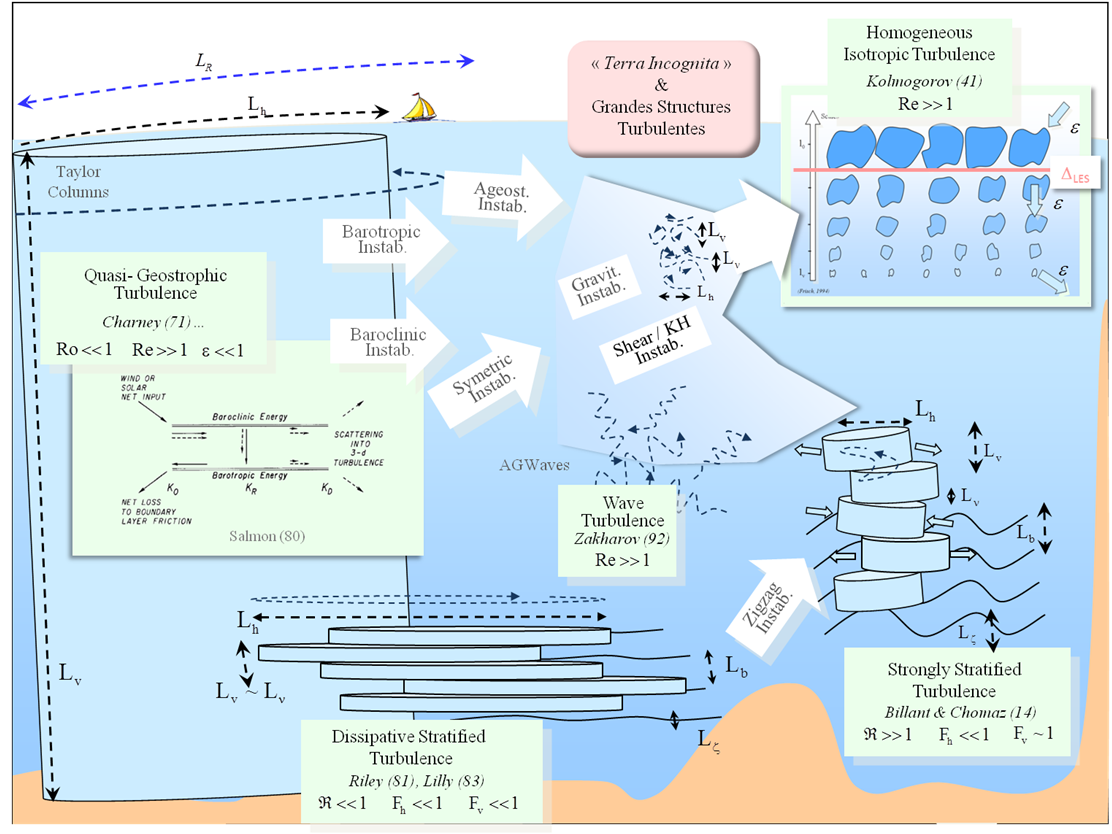
\includegraphics[width=0.8\textwidth]{./INTRO/Ocean_scales.png}
  \caption{\color{red}l'océan vu à travers ses cascades d'échelles, ses instabilités et ses principaux modèles de turbulence.\color{black}}
  \label{fig_ocean_scales}
\end{figure}
%\color{blue}
L'océan est soumis à/ mis en mouvements sous l'action de nombreux forçages par la pression atmosphérique, les marées astronomiques ou les flux de quantité de mouvement induits par le vent mais aussi par les flux de chaleur radiatifs ou par les flux de chaleur latente ou encore par les précipitations, les fleuves ou encore par évaporation... Ainsi présenté, l'océan peut donc être présenté comme un \textit{système dynamiquement ouvert}, l'ensemble des forçages auxquels il est soumis induisant un large spectre de processus dynamiques: houle, courants d'Ekman, upwelling ou downwelling, ondes de marée, marées internes, convection profonde, courants de gravité, panaches fluviaux... 


La dynamique de l'océan est variée, composée de processus dynamiques couvrant une large gamme autant spatiale que temporelle. La houle, les courants d'Ekman, les systèmes d'upwelling ou de downwelling, les ondes de marée, les marées internes, la convection profonde, les courants de gravité, ou encore les panaches fluviaux, 

, composée d'une large gamme de processus aux extensions géographiques 


%d'un large spectre de processus, on peut citer la houle, les courants d'Ekman, les systèmes d'upwelling ou de downwelling, les ondes de marée, les marées internes, la convection profonde, les courants de gravité, ou encore les panaches fluviaux... 

L'océan ne se résume toutefois pas à une somme de processus "forcés" dont la combinaison linéaire suffirait à expliquer sa dynamique propre. Ces processus interagissent en effet entre eux induisant d'importants \textit {mécanismes de transferts} entre les différentes gammes d'échelles spatiales et temporelles. Lorsque ces transferts prennent une forme cohérente dans quelques régions spécifiques du spectre, on parle de \textit{cascades d'échelles}. Les mécanismes débouchant sur ces transferts sont quant-à eux généralement associés à des \textit{instabilités dynamiques}.\\
\cite{salmon_baroclinic_1980} montrent par exemple qu'à méso-echelle\footnote{Région du spectre constitué d'échelles plus grande que le premier rayon de Rossby.} ces transferts s'organisent de façon cohérente sous la forme d'une \textit{cascade inverse} associée à des transferts énergétiques barotropes dirigés majoritairement vers les plus grandes échelles\footnote{Une telle cascade "inverse" est caractéristique de régimes de turbulence 2D.} alors que les transferts d'enstrophie\footnote{A l'image de l'énergie cinéatique cinétique pour la vitesse, l'enstrophie est définie comme la moitié du carré de la vorticité relative, i.e. du rotationnel de la vitesse.} sont quant à eux majoritairement dirigés vers les plus fines échelles. 
Les vents et les flux de chaleur induisent ainsi des structures dynamiques (baroclines) qui sont brisées lorsque l'écoulement devient instable \citep{vallis_atmospheric_2006}.
Les \textit{instabilités barotropes et baroclines} sont par conséquent au coeur de cette cascade dite inverse, elles rythment les transferts autour des rayons de Rossby\footnote{Échelle caractéristique de longueur caractérisant localement l'impact de la rotation du globe terrestre sur une colonne océanique de stratification donnée.} barotropes et baroclines dans les écoulements de mésoéchelles. On parle de régime de \textit{turbulence géostrophique} \citep{charney_geostrophic_1971} dans une région du spectre où stratification de la colonne d'eau et rotation du globe terrestre jouent \textit{in fine} des rôles prépondérants et sont associés à des équations de bilan équilibrées de quantité de mouvement. La cascade inverse demeure toutefois un modèle qualitatif fournissant une grille de lecture pour processus complexes et "non localisés" du le spectre océanique.\\
Des structures de sous-mésoéchelle reçoivent ainsi énergie et enstrophie et sont elles-aussi sujettes à un large éventail d'instabilités \citep{mcwilliams_submesoscale_2016}: instabilité agéostophique, symétrique, frontale, convective ou encore instabilités de cisaillement, instabilités baroclines dans la couche de mélange océanique, instabilités paramétriques des ondes internes... Dans cette région du spectre, l'impact de la rotation du globe terrestre est plus faible qu'à mésoéchelle mais la stratification contraint fortement la dynamique océanique débouchant sur des formes de turbulence dites "stratifiées": \textit{turbulence stratifiée dissipative}, \textit{turbulence fortement stratifiée}. l'instabilité "zig-zag" fait office de pont entre ces deux formes de turbulence).\\
Les myriades d'ondes de gravité internes et d'ondes de gravité de surface interagissent aussi au point de donner lieu à une forme particulière de turbulence: \textit{la turbulence d'onde}. Leur déferlement, leurs instabilités donnent généralement naissance à des "patchs turbulents" annoncés par l'apparition de grandes structures turbulentes.\\
En deçà de cette mésoéchelle (on parle de sous-mésoéchelle), prend naissance une autre cascade présentant une certaine cohérence, la \textit{cascade directe} ou cascade de Richardson au sein de laquelle l'énergie est transférée "directement" vers l'échelle de Kolmogorov au delà de laquelle la dissipation moléculaire est active. Si les théories décrivant les transferts à mésoéchelles ne permettent pas de routes directes vers la dissipation, les transferts de sous-mésoéchelle le permettent.
Les \textit{grandes structures turbulentes} marquent l'entrée de cette cascade directe, elles sont associées à des instabilités de cisaillement telles que les instabilités de Kelvin-Helmholtz. A \textit{micro-échelle}, le modèle de turbulence homogène et isotrope 3D décrit de façon simple cette cascade. Les échelles spatiales et temporelles des grandes structures turbulentes ne sont toutefois pas clairement définies: elles peuvent atteindre quelques dizaines de mètres au sein de la colonne d'eau mais peuvent aussi ne pas dépasser le mètre dans les couches de surface ou de fond.\\
Cascades d'échelles et modèles de turbulence décrivent ainsi des régions spécifiques du spectre spatio-temporel de l'océan qui présentent une certaine cohérence. Les divers types d'instabilités tissent quant-à elles des ponts entre ces régions. En toute rigueur, comprendre, expliquer, simuler (explicitement) ou modéliser (implicitement) le mélange turbulent, impliquent donc évidemment de représenter correctement l'ensemble du spectre océanique, ses transferts, ses cascades... Elle requière toutefois plus spécifiquement de reproduire précisément la cascade turbulente directe, i.e. le transfert "inertiel" d'énergie aboutissant à la région "dissipative" du spectre. Le point de départ de cette cascade n'est cependant pas clairement défini et varie aussi bien dans le temps que dans l'espace. Seule l'apparition souvent intermittente de grandes structures turbulentes permet de localiser spatialement et temporellement ce point de départ.\\
%Les grandes structures turbulentes marquent donc l'entrée de la cascade directe menant à la dissipation moléculaire. Elles sont ainsi à l'origine d'une cascade débouchant sur une réorganisation irréversible, diabatique de la colonne d'eau et d'un redistribution des "traceurs" passifs ou actifs. Parmi ces "traceurs", la masse volumique joue un rôle particulier dans la dynamique océanique: les masses d'eau sont par exemple "transportées" le long des surfaces isopycnales et le contenu en vorticité potentielle entre deux de ces surfaces isopycnales se conserve au cours du temps.\\
A. Scotti \citep{scotti_large_2010}, dans une revue sur la modélisation de l'océan, conclut qu’avec l'étude des grandes structures turbulentes, s'ouvrent les portes de la \textit{terra incognita}. Il reprend ainsi la conclusion de J.C. Wyngaard \citep{wyngaard_toward_2004} rédigée quelques années auparavant pour l'atmosphère. Cette terre inconnue, souvent aussi qualifiée de "zone grise" abritant les \textit{fines échelles océaniques}, est plus largement considérée comme la région particulièrement mal connue du spectre océanique dans laquelle la dynamique peut localement et temporairement basculer d'un équilibre simple entre un nombre limité de processus vers une dynamique non-linéaire complexe induisant une cascade d'instabilités dynamiques (directe) aboutissant à la dissipation moléculaire. 
\color{black}
%Cependant, l'océan (tout comme l'atmosphère) a un écoulement turbulent, c'est-à-dire chaotique et non-linéaire/ constitué d'une intéraction d'échelle.
%...
%Cette turbulence se manifeste en la décomposition des structures de grande échelles/synoptiques en des champs de plus petite structures/structures de plus en plus petites (transiant?) en intéractions les unes avec les autres (tourbillons, etc). Ainsi l'étude de l'océan peut se faire à bien des échelles spatiales et temporelles
%Ce manuscrit de thèse porte sur l'étude d'une dynamique dite de 'fine échelle', sur les processus / phénomènes océaniques . Il s'agira 
\color{blue}
\subsection{Rétroactions}
\label{subsection_retroactions}
Le mélange peut ainsi être présenté comme l'aboutissement de transferts et de cascades plus ou moins cohérentes mais quoiqu'il en soit très hétérogènes et intermittentes. Il ne constitue toutefois pas un puits sans fond ou un aller sans retour. Les flux diapycnaux modifient en effet les masses d'eau, la dissipation visqueuse qui "injecte" de la vorticité potentielle\footnote{La vorticité potentielle est une quantité, une substance d'après \cite{haynes_conservation_1990}, essentielle dans la description des écoulements stratifiés et en rotation qui est conservée par advection} près du fond... et constituent donc autant d'exemples de retroaction sur la grande échelle.\\
\cite{penney_2020} ont montré que le mélange était finalement capable de structurer les plus grandes échelles en mettant en évidence l'apparition à plus grande échelle de relations linéaires entre la masse volumique et les traceurs passifs qu'ils simulent.\\
La région du détroit de Gibraltar séparant la mer Méditerranée de l'océan Atlantique est à ce titre tout à fait exemplaire. Les masses d'eau méditerranéennes et atlantiques s'y croisent de façon tout aussi éphémère que brutale. Le mélange de ces deux masses d'eau induit par les fortes amplitudes de marée modifient in fine la salinité ou la quantité de mouvement de ces masses d'eau exerçant un contrôle sur la dynamique de l'ensemble du bassin Méditerranéen \citep{armi_1988}, scellant en quelques sortes le régime dynamique de l'ensemble du bassin et fixant vraisemblablement le contenu en vorticité potentielle du jet méditerranéen en Atlantique Nord.\\
La dissipation turbulente exerce donc une rétroaction sur les plus grandes échelles du spectre océanique: elle  structure les masses d'eau mais aussi la circulation océanique.
\color{black}
%(Revient plus en détail sur la turbulence, cas où mot est utilisé (turbulence géostrophique? vs cascade turbulente))
%Turbulence de mésoéchelle (instabilité barocline), ici on s'intéresse au début de la cascade turbulente directe définie par Kolmogorov. Les 2 sont similaires en ce qu'elles concernent le transfert d'énergie vers de plus fines échelles. Pour le cas de la turbulence de fine échelle, // mais va aussi aboutir à structuration de l'écoulement en lui-même. (La conservation de la vorticité potentielle (PV) peut agir comme un effet structurant de jet/courants...//méandres d'un jet / courant structurés par la conservation de la vorticité potentielle... PV générée par diabatic processes (in boundary layers?)...

%Cascade inverse???

\subsection{Le détroit de Gibraltar}
%(intérêt de la zone en vu du blabla précédent)
\color{blue}
Les talus continentaux, dorsales océaniques, les monts sous-marins isolés et autres détroits sont autant d'accidents bathymétriques qui canalisent, perturbent, modifient la circulation générale des masses d'eau océaniques et plus généralement la dynamique de l'océan. Les accidents bathymétriques sont localement le siège de régimes de couches limites particuliers entraînant quasi-systématiquement l'apparition de structures turbulentes très localisées spatialement et ouvrant ainsi les portes de la "terra incognita".\\
Le détroit de Gibraltar déjà cité dans le paragraphe précédent (\S \noparref{subsection_retroactions}) comme exemple de région abritant des processus de fine échelle structurant la dynamique océanique de grande échelle, constitue l'archétype de l'accident topographique contraignant fortement la dynamique océanique. Il est en effet le lieu de passage obligé des échanges entre les bassins méditerranéens et atlantiques nord.\\
\color{red}
Je te laisse compléter avec une présentation de la dynamique de cette région : marée + circulation générale => ressaut + ISW +... fort mélange.\\
\color{blue}
La dissipation turbulente est répartie de façon très hétérogène dans la colonne d'eau océanique, souvent préférentiellement dans les couches de surface et de fond et généralement sous la forme d'évènements intermittents (on parle de bouffées turbulentes). Ces caractéristiques compliquent grandement sa localisation et sa quantification même si son impact sur la circulation générale est maintenant reconnu et décrit de façon très qualitative \cite{de_lavergne_abyssal_2017}. La région du détroit de Gibraltar offre donc un terrain d'étude particulièrement pertinent pour qui souhaite étudier cette dissipation turbulente et ses rétroactions puisque les bouffées turbulentes semblent devoir être associées aux régimes dynamiques présentant de fortes amplitudes de marée (donc facilement localisables dans le temps) et au dessus des principaux seuils parsemant le détroit (donc facilement localisables géographiquement cette fois).\\
Le choix du détroit de Gibraltar comme région d'étude privilégiée pour mes travaux de doctorat se justifie donc à plusieurs titres. Elle est particulièrement adaptée pour une première exploration en \textit{terra incognita} puisque quelques portes ouvrant une voie vers cette terre inconnue semblent y être facilement localisables: les grandes structures turbulents peuvent être un peu plus facilement localisables, observables et donc simulées explicitement de façon numérique. Le détroit de Gibraltar est de plus une région de choix pour mieux appréhender l'impact (la rétroaction) que pourrait avoir la dissipation turbulente sur la circulation générale dans les bassins méditerranéens et nord-atlantiques: il s'agit donc d'une région de choix pour étudier comment cette dissipation peut structurer une dynamique à beaucoup plus grande échelle.
\color{black}

\color{blue}
\section{Une exploration des fines échelles océaniques}
%\color{red}
%(verrous puis objectif)
\subsection{Définir cette région du spectre océanique}
Objet central de mes travaux de doctorat, les \textit{fines échelles} océaniques doivent en premier lieu être clairement définies. Jusqu'ici, ces fines échelles ont plus spécifiquement été associées dans notre introduction (\S \noparref{subsection_intro1}) à la région du spectre océanique identifiée comme \textit{Terra incognita}.\\
Les fines échelles sont donc par la suite définies comme les échelles spatiales et temporelles de l'ensemble des processus et autres mécanismes dynamiques de \textit{sous-mésoéchelle} \citep{mcwilliams_submesoscale_2016} auxquels s'ajoutent les grandes structures turbulentes ouvrant la voie à la cascade directe et marquant l'entrée de la \textit{micro-échelle}.
 \color{black}

\subsection{Se donner les outils et les moyens d'une telle exploration}
\color{blue}
Toute entrée dans un territoire inconnu tel que la \textit{terra incognita} est associée à la reconnaissance et à la levée d'un certain nombre de difficultés. Dans le cas présent, ces "difficultés" prennent la forme de véritables \textit{verrous} d'ordres dynamiques et numériques.
\subsubsection{Verrous dynamiques.}
Un certain nombre de "verrous" dynamiques peuvent être identifiés. Les grandes structures turbulentes dont il est en particulier question ici sont le résultat de diverses instabilités "primaires" peuplant la méso et la sous-méso-échelle océaniques: instabilités barotrope, barocline, symétrique, zig-zag, agéostrophique, paramétrique des ondes internes, etc... Ces mécanismes de déstabilisation peuvent être vus comme brisant des structures, des processus, des équilibres subtils régissant localement et de façon éphémère et intermittente la dynamique de l'océan. Leur exploration relève par conséquent plus d'une approche stochastique que purement déterministe.\\
Les grandes structures turbulentes constituent de plus des processus certes importants mais néanmoins indissociables des transferts d'échelles auxquels elles sont associées. Leur étude requiert donc la prise en compte simultanée de régions étendues du spectre océanique.\\
Ni les échelles spatiales ni les échelles temporelles des instabilités de cisaillement ne sont clairement identifiables à partir de grandeurs caractéristiques comme le peuvent être les rayons de Rossby pour la méso-échelle et les instabilités barotropes et baroclines.
\subsubsection{Verrous numériques.}
Les grandes structures turbulentes étaient traditionnellement l'apanage des modèles "sous-maille" dans les configurations océaniques côtières, régionales et à fortiori globales. N'étant par conséquent pas universels, ces modèles "sous-maille" rendent la simulation très dépendante du lieu et de la période étudiés: les "modèles de fermeture" doivent en effet être ajustés et confrontés à la réalité avec comme principal enjeu le choix du modèle et la détermination des paramètres physiques ou numériques qu’il inclut nécessairement. Si la réalisation de LES est envisageable et envisagées dans l’océan intérieur et peut donc être appuyée sur des modèles de turbulence plus universels et plus simple, elle demeure par contre hors d’atteinte dans les couches limites de surface et fond, régions dans lesquelles leurs échelles spatiales caractéristiques peuvent considérablement décroître pour être finalement de l'ordre du mètre. Des approches dites "zonales" doivent par conséquent être envisagées.
La simulation explicite des grandes structures turbulents engendre l'utilisation de grilles de calcul à très haute résolution sur des régions océaniques à priori relativement étendues. Elle requière donc un nouvel effort de réduction du coût de calcul. CROCO est en effet conçu et développé pour être un code efficace mais ce qu'il est aujourd'hui possible de simuler explicitement dans un détroit d'extension réduite doit être généralisé à des sous-bassins et à des plateaux continentaux de plus grande extension avec, très vraisemblablement, une résolution raffinée. Nous avons mené à bien une première étude de faisabilité au sein de notre petit groupe CROCO / LA débouchant sur le portage du code sur GPU sur des machines hétérogènes CPU / GPU. Le nécessaire travail d’optimisation des performances est désormais en conduit en très étroite collaboration avec les équipes INRIA. Le surcoût de calcul associé à la compressibilité et à la remise en cause de l'hypothèse hydrostatique a par exemple dors et déjà pu être effacé en déportant sur GPU l'intégration du mode rapide compressible.


\color{black}
\subsection{Simuler explicitement les fines échelles}
\color{blue}
Explorer numériquement les fines échelles océaniques implique de simuler explicitement les grandes structures turbulentes et l'on entre ainsi de plain-pied dans une approche numérique dite \textit{LES (pour \textit{Large Eddy Simulation})}.\\
La promesse d’une puissance de calcul pétaflopique puis exaflopique a, en théorie au moins, ouvert les portes de la simulation des grandes structures turbulentes (LES) pour l’océan et l’atmosphère. Les météorologues ont par exemple rapidement su tirer parti des moyens de calcul disponibles : des algorithmes dédiés ont vu le jour dès le début des années 2000 débouchant sur des codes numériques tels que WRF en version compressible ou Méso-NH en version anélastique. Ces deux types de codes permettent, chacun avec leurs spécificités, d’aborder la simulation de la cascade turbulente directe en représentant explicitement les plus grandes structures turbulentes dans l’atmosphère.
Les modèles océaniques n’ont pas été immédiatement en mesure de franchir ce cap de la LES en grande partie à cause de la présence d’une surface libre aux conséquences dynamiques multiples. La surface libre rend en particulier plus complexe la relaxation de l’hypothèse hydrostatique. Dans la foulée de l’ANR COMMODO rassemblant au milieu des années 2010 l’ensemble des équipes françaises travaillant sur la modélisation de l’océan, les équipes de recherche en océanographie dynamique et en mathématiques partenaires du projet CROCO se sont associées pour développer une nouvelle génération de codes capables d'explorer la "Terra Incognita". Un Groupement de Recherche éponyme est né associant l’université de Toulouse et les principaux organismes de recherche en informatique et en océanographie français: l’IRD, INRIA, le CNRS-INSU, l’IFREMER et le SHOM. En 2021, l’IRD a entériné la constitution d’un GdRi CROCO tourné vers nos partenaires au Sud.\\
Plusieurs pré-requis ont toutefois dû être satisfaits avant de lancer une exploration numérique des grandes structures turbulentes dans un contexte réaliste aussi complexe que celui du détroit de Gibraltar.
L'hypothèse hydrostatique, elle-aussi héritée du code ROMS, devait à minima être remise en cause en demeurant dans le contexte d'un océan à surface libre. Ceci fut chose en fait en relaxant aussi l'hypothèse de Boussinesq comme préconisée dans un contexte océanique par \cite{auclair_non-hydrostatic_2018}. L'héritage reçu du code américain ROMS \citep{shchepetkin_regional_2005} avait fait de CROCO un code particulièrement efficace dont le coeur numérique (son time-splitting, ses schémas numériques...) a été spécifiquement conçu pour limiter les coûts de calcul et l'utilisation de l'espace mémoire. Ce niveau de performance numérique a été maintenu pour son noyau numérique compressible et non-hydrostatique dans un contexte massivement parallèle.\\
De nouvelles recherches ont été entamées en parallèle de mes travaux de thèse pour d'une part porté sur le code sur une nouvelle génération de processeurs dits hétérogènes (associant CPU et GPU) et d'autre part permettre le raffinement local de la dynamique océanique par imbrication de configurations LES dans des maquettes numériques régionales très étendues. Les maquettes que j'ai développées ou co-développées dans le cadre de mes travaux de thèse ont servi de configuration-tests pour l'ensemble de ces développements transformant le détroit de Gibraltar en une région de démonstration.\\
\color{blue}
\subsection{Où l'on justifie une démarche scientifique pour cette exploration...}
\color{black}
Les années de thèse ont eu pour objectif de mettre en place outil sur une région particulièrement/// Simuler explicitement, observer, quantifier, pour explorer intéraction d'echelles sur spectre élargi


\section{Plan du manuscrit}




%Morceaux de intro GBR3D : 
%The amplitude of the exchange varies over timescales larger than the semi-diurnal tide. The lower frequencies (whether seasonal or inter-annual) are usually linked to atmospheric forcing over the Mediterranean \citep{sanchez-roman_2012}. The tidal eddy-fluxes have their own variability associated to the spring-tide cycle and to the monthly tides, with for example a greater depth and stronger shear during neap tides, but more intense mixing during spring tide \citep{naranjo_2014,vargas_2006}.\color{red}(enlever? sert à rien? que dans intro plus générale???)\color{black}


%Numerical models are discretized and have a treshold resolution under which phyisical pehomenons cannot be represented explicitely. Particularly, diffusion and ... processes,  among other parametrisations of processes like surface exchanges, radiation that occur at molecular or submolecular scales. Diffusion and dissipation are molecular in nature as a , energy flux, but more broadly speaking, dissipation is the transfer of energy from great scales to small scales. In a stratified fluid, this dissipation is accompagnied by mixing , ie a lewoering of potential energy, or more accurately and explained i paragraph ..., of the background potential energy.
%Broadly for oceanic (or more generally geophyisic?) models classification on DNS, LES, and RANS. DNS has molecular dissipation
%For the discussions simply coining as LES is not sufficient but need to precise LES in regard to which phenomenon. For exemplein chapoter ... of this manuscript, coined LES because primary instabilities of the flow. However, the primary instabilities that are known to exist at upper and lower boundaries of teh water column are not represented and are parametrized, so in regard to the dissipation those process not LES. 
%To this considerations, one must also not forget that the discretisation itself introduces numerical dissipation unless using centered schemes (computationnally impossible).



%\subparagraph{Conclusion générale/dans le manuscrit}
%Les simulations ... sont première LES maisblablablablabla (trad ce que avait dit...). Besoin outil diagnostique du mélange, chapitre prochain...





%%%%%%%%%%%%%%%%%%%%%%%%%%%%%%%%%%%%%%%%%%%%%%%%%%%%%%%%%%


\chapter{Mod\'elisation  Repr\'esentation de l'oc\'ean et de son m\'elange}
\begin{itemize}
\item conservation masses/qdm, discretisation numérique, échelles (RANS/LES(/DNS)), paramétrisation du mélange, fermeture turb (Smago/GLS...)
\item contenu en PV
\item definition BPE, eq d'évolution 'générale'
\item code CROCO (ou code CROCO en premisce de chap 3 GBR2D????(sinon parait cours?)GBR2D parle passage hydro a NBQ...)
\end{itemize}



\section{Résumé du chapitre en français}
Le présent chapitre présente de façon détaillée le \textit{modèle d'océan} utilisé dans le cadre de ma thèse pour simuler numériquement les grandes échelles turbulentes (ou LES$^{\noparref{LES}}$) dans la région du détroit de Gibraltar mais aussi, plus généralement, pour développer des modèles analytiques simplifiés de processus au service de cette approche numérique. Plusieurs sections du chapitre ont été intégrées à des publications acceptées \citep{hilt_2020}, \citep{auclair_modied_2021} ou en cours de rédaction  \citep{auclair_NBQ1_2021} mais aussi au rapport d'études du programme amont PROTEVS Gibraltar du SHOM \citep{auclair_modelisation_2019}. L'ensemble du chapitre est par conséquent rédigé en anglais.

Dans une première partie (\S \ref{section_prim_eq}) sont introduites les équations de conservations usuelles de l'océanographie physique, dont les équations de Navier-Stokes, point de départ du développement du \textit{modèle d'océan}. Le choix est ensuite fait de se placer dans le contexte d'une grille verticale curviligne qui permet d'épouser la forme des fonds marins et de suivre les mouvements de la surface libre de l'océan (dont un certain nombres de développements ont aussi présentés en annexe (\noparref{section_annexe2})). 
%Dans ce cadre, l'expression de l'évolution de l'énergie potentielle gravitationnelle (PE) et de ses sous-compartiments, énergie potentielle disponible (APE) et énergie potentielle de "background" (BPE), est développée dans un volume local d'océan (section \ref{section_PE_chap2}). En particulier, l'évolution de la BPE fait apparaître un terme source lié aux mouvements de la surface libre. Comme l'évolution de la BPE est lié au mélange diapycnale, la bonne expression de son bilan est impérative afin de faire des diagnostics de quantifications de mélange se basant sur cette méthode. %FA%

Dans la deuxième partie du chapitre (section \ref{section_croco}), est présenté le fonctionnement du code communautaire à cœur non-hydrostatique, compressible et à surface libre CROCO, basé sur le \textit{modèle d'océan} de la première partie. 
L'implémentation numérique de ce \textit{modèle d'océan} a demandé d'importants développements tant algorithmiques que numériques, développements qui ne peuvent être menés à bien s'ils miment directement la physique de l'océan. Parce qu'il est très général, ce \textit{modèle d'océan} peut réaliser la synthèse de processus dynamiques dans une gamme très étendue d'échelles spatio-temporelles depuis la circulation basse fréquence, jusqu'aux ondes acoustiques. Ce sont plus spécifiquement les plus fines échelles et les plus hautes fréquences qui peuvent imposer les plus fortes restrictions à l'approche numérique envisagée ; ce sont donc les processus associés et en particulier les processus ondulatoires acoustiques ou gravitaires qui ont été étudiés en priorité. 

%Ce \textit{modèle d'océan} est suffisamment général pour autoriser la représentation explicite d'une large gamme de processus allant des ondes et modes acoustiques dans un océan compressible aux structures turbulentes fondamentalement non-hydrostatiques de \textit{fine échelle} (associées par exemple à des instabilités de Kelvin-Helmholtz) en passant par des processus ondulatoires internes de grande amplitude (tels que les solitons).

J'ai participé à une partie des développements de CROCO durant ma thèse, sur le plan purement numérique tout d'abord, avec l'implémentation et l'évaluation de nouveaux schémas numériques dans un contexte pleinement réaliste et la mise en œuvre de stratégies originales pour la LES. Sur le plan de la dynamique océanique ensuite, avec la réalisation d'études de processus de fines échelles et l'étude des interactions complexes entre ces processus.

%Ce \textit{modèle d'océan} a de plus servi de base au développement dans le cadre de ma thèse de diagnostiques originaux dédiés à la simulation des grandes échelles turbulentes océaniques (LES) dans un contexte réaliste: évaluation quantitative du mélange turbulent (\S \noparref{chapter_bpe}), mise en évidence et caractérisation de ces structures, études de ressauts hydrauliques (\S \noparref{PartDiag3D})...

En parallèle des développements numériques et des travaux sur la dynamique de la région du détroit de Gibraltar menés dans le cadre de la présente thèse de doctorat, a été développé et publié un modèle analytique suffisamment général pour décrire la dispersion des ondes et des modes acoustiques, des ondes et des modes internes de gravité ou encore des ondes de gravité de surface \citep{auclair_modied_2021}. Le modèle analytique de dispersion a de plus été utilisé pour explorer la dynamique ondulatoire dans la région du détroit de Gibraltar.
J'ai participé et co-signé cette étude en support du développement numérique de CROCO, étude qui n'a pas été incluse dans le présent manuscrit.

Dans ce qui suit du présent chapitre, c'est l'anglais qui est utilisé pour les raisons évoquées précédemment.

%Dans une première partie, les équations analytiques servant de base à ce \textit{modèle d'océan} sont présentées (\noparref{section_prim_eq}), l'approche numérique choisie et co-développée pour le coeur numérique non-hydrostatique, compressible et à surface libre de CROCO est détaillée en partie \ref{section_croco}. Un certain nombre de développements sont enfin présentés dans les annexes (\noparref{section_annexe2}).


\section{A non-hydrostatic, compressible, free-surface ocean model}
\label{section_prim_eq}

%%%%%%%%%%%%%%%%%%%%%%%%%%%%%%%%%%%%%%%%%%%%%%%%%%%%%%%%%%%%%%%%%%%%%%%%%%%%%
 %----------------------------------------------------------------------------
 \subsection{Continuous free-surface compressible equations in z-coordinates}
 %----------------------------------------------------------------------------
\label{subsectiongenesystem}
\subsubsection{Model equations in conservative form}
Conservation of mass, conservation of momentum (Newton's second law of motion), conservation of total energy (first law of thermodynamics) and conservation of any tracers are the backbones of ocean dynamics. In the ocean, the conservation of mass can be written as a prognostic equation for density (written $\rho$), the conservation of momentum leads to prognostic equations for the three components of momentum (written $\rho \mathbf{v}$) and the conservation of total energy (or first law of thermodynamics) can be stated as a prognostic equation for potential temperature ($\theta$). The conservation of chemical species can then be expressed as a prognostic equation for salinity ($S$). These conservation equations consequently lead to the following general system of prognostic equations (expressed in flux form):
\begin{subequations}
 \begin{alignat}{2}
 \displaystyle
 \label{NS_a} 
 & \frac{\partial\rho}{\partial t} &&= - \mathbf{\nabla}\cdot(\rho \mathbf{v})\\[3mm]  
 \label{NS_b}
 & \frac{\partial \rho \mathbf{v}}{\partial t} 
	 &&= -\mathbf{\nabla}\cdot(\rho \mathbf{v}\otimes \mathbf{v}) 
	  \color{black} -2\rho\ \mathbf{\Omega}\ \times \ \mathbf{v} \color{black} -\mathbf{\nabla}p + 		
	\mathbf{\nabla}\cdot\left(
	\mu(\mathbf{\nabla}\mathbf{v}+\mathbf{\nabla}\mathbf{v}^{\ T})
 +\mu_2(\mathbf{\nabla}\cdot\mathbf{v})\ \mathbf{I}\ \right)
 +\rho \mathbf{g}\\
 %
 \label{NS_c}
 & \frac{\partial \rho \theta}{\partial t} &&=-\mathbf{\nabla}\cdot(\rho \theta\mathbf{v})
 +\mathbf{\nabla}\cdot\color{black}(\kappa_\theta\mathbf{\nabla}{\theta})\color{black}\\[3mm]
 %
 \label{NS_d}
 & \frac{\partial \rho S}{\partial t} &&=-\mathbf{\nabla}\cdot(\rho S\mathbf{v})
 +\mathbf{\nabla}\cdot\color{black}(\kappa_S\mathbf{\nabla}{S})\color{black}
 %
  \end{alignat}
\end{subequations}
with $\mu$, $\mu_2$, $\kappa_T$ and $\kappa_S$ respectively the dynamical and bulk viscosities and the thermal and salt diffusivities. $\mathbf{\Omega}$ is the earth instant rotation vector.
Assuming that variables are in thermodynamic equilibrium, the equation of state (EOS) can be formulated as a non-linear, diagnostic functional relation between temperature, salinity, density and (total) pressure (written $p$):
\begin{equation}
 \label{NS_e}
 \rho = \rho_{eos}[\theta,S,p]
\end{equation}

\subsubsection{Boundary conditions}
The position of the interface separating the ocean and the atmosphere must additionally be calculated and is introduced as a boundary condition. This can be achieved by stating that a salty-water particles that is just bellow this interface in the ocean, remains at the interface, leading to the surface kinematic relation:
\begin{equation}
  \displaystyle
  \label{NS_BC2}
  %\frac{\textrm{d}\zeta(\mathbf{x}_{\scriptscriptstyle H},t)}{\textrm{dt}}=w(\mathbf{x}_{\scriptscriptstyle H},z=\zeta)
  \frac{\partial \zeta}{\partial t}=w(\mathbf{x}_{\scriptscriptstyle H},z=\zeta)-\mathbf{v}_H(\mathbf{x}_{\scriptscriptstyle H},z=\zeta)\cdot\mathbf{\nabla}_H\zeta
\end{equation}
where $\zeta$ is the free-surface anomaly in the vicinity of the geoid and subscribe $H$ indicates that only the horizontal component is considered. Assuming then that ocean water cannot penetrate the ocean bottom (at depth $z=-H$):
\begin{equation}
 \displaystyle
 \label{NS_BC0}
  \mathbf{v}(\mathbf{x}_{\scriptscriptstyle H},z=-H)=\mathbf{0}
\end{equation}
Neglecting surface-tension pressure drop, the boundary condition for pressure at the surface of the ocean is given by:
\begin{equation}
 \displaystyle
 \label{NS_BC1}
  p(\mathbf{x}_{\scriptscriptstyle H},z=\zeta,t)= p_{atm}
\end{equation}
with $p_{atm}$ the atmospheric pressure above the surface of the ocean.
The resulting system of prognostic equations, diagnostic relations and boundary conditions leads to a non-linear problem whose main characteristics is the wild spectrum of dynamic processes involved (see for instance \cite{gill_atmosphere-ocean_1982} or \cite{vallis_atmospheric_2006}). Periodic processes such as ocean waves can give a comprehensive overview of the extension of space-time spectrum of transient processes which can propagate in the ocean and \cite{auclair_modied_2021} derive a compressible, free-surface, stratified model of two dispersion relations for wave-numbers and pulsation gathering acoustic, surface and internal waves and insisting on the modification of the dispersion of gravity (acoustic) waves by compressibility (gravity and stratification).

Formulated thus, the system of Navier-Stokes and conservation equations for a free-surface ocean can, at least in theory, be integrated straightforwardly. All variables but the pressure have their own prognostic equation and pressure can be diagnosed from the EOS \ref{NS_e}. Note that the system can be reformulated so that pressure is also given by a prognostic equation.

\subsubsection{Evolution of the density field}
For a linear approximation of the equation of state, a simple evolution equation of $\rho$ can be obtained as a combination of equations \ref{NS_c} and \ref{NS_d} leading to:
\begin{equation}
\displaystyle
\frac{d \rho}{d t}=
%\frac{\partial}{\partial x} \bigg(\kappa_\rho^h \frac{\partial \rho}{\partial x}\bigg\rvert_{tz}\bigg)_{tz}
%+ \frac{\partial}{\partial z} \bigg( \kappa \frac{\partial \rho}{\partial z}\bigg\rvert_{tx}\bigg)_{tx} 
 \mathbf{\nabla}\cdot\color{black}(\kappa_{\rho} \mathbf{\nabla}{\rho})
\label{eq_diff_cart}
\end{equation}
where $\kappa_{\rho}$ is the equivalent diffusivity of density.

 %----------------------------------------------------------------------------  
 %\subsection{Density and pressure decomposition}
 %----------------------------------------------------------------------------
 
\subsection{Terrain-following coordinates}
\label{subsection_scoord}

 %%%%%%%%%%%%%%%%%%%%%%%%%%%%%%%%%%%%%%%%%%%%%%%%%%%%%%%%%%%%%%%%%%%%%%%%%%%%%
\subsubsection{Definition}
%%%%%%%%%%%%%%%%%%%%%%%%%%%%%%%%%%%%%%%%%%%%%%%%%%%%%%%%%%%%%%%%%%%%%%%%%%%%%
The capacity of numerical models to mimic the evolution of global or regional oceanic circulation relies on horizontal and vertical definition of the grid on which the Navier-Stokes and conservation equations previously defined are solved and integrated in time.

Due to considerations of the representation of bathymetric features and free-surface evolutions, terrain-following coordinates, or S-coordinates, are chosen for the vertical discretisation. They are generally defined on generalized constant-$s$ surfaces with $s$ given by:
\begin{equation}
 \displaystyle
 s=s(x,y,z,t)=s(\mathbf{x},t)
\end{equation}
requiring thus that $s$ be a monotonic function of the vertical coordinate $z$:
\begin{equation}
 \displaystyle
 \frac{\partial s}{\partial z}\bigg\vert_{xyt}\ne 0
\end{equation}
$\partial s / \partial z$ is continuous and single-signed (either strictly positive or negative).

%%%%%%%%%%%%%%%%%%%%%%%%%%%%%%%%%%%%%%%%%%%%%%%%%%%%%%%%%%%%%%%%%%%%%%%%%%%%%
\subsubsection{Examples}
%%%%%%%%%%%%%%%%%%%%%%%%%%%%%%%%%%%%%%%%%%%%%%%%%%%%%%%%%%%%%%%%%%%%%%%%%%%%%
Several examples and comparisons on the choice of $s(\mathbf{x},t)$ are given in chapter 6 of \citet{griffies_fundamentals_2004}.
Following  \citet{shchepetkin_regional_2005},  less general $\sigma$-coordinates can be defined by:
\begin{equation}
 \displaystyle
 z(\mathbf{x},\sigma,t)=\sigma H(\mathbf{x_h})\quad or\quad z(\mathbf{x},\sigma,t)=\sigma(H(\mathbf{x_h})+\zeta(\mathbf{x_h},t))+\zeta(\mathbf{x_h},t)
\end{equation}
%or:
%\begin{equation}
% \displaystyle
% z(\mathbf{x},\sigma,t)=\sigma(H+\zeta)+\zeta
%\end{equation}
where $H(\mathbf{x_h})=H(\mathbf{x,y})$ is the bottom topography and $\zeta(\mathbf{x_h},t)$ the surface elevation anomaly. Its generalization to s-coordinates is defined by:
\begin{equation}
 \displaystyle
 z(\mathbf{x},s,t)=\mathcal{S}(s) H(\mathbf{x_h})
\end{equation}
which is currently written:
\begin{equation}
 \displaystyle
 z(\mathbf{x},\sigma,t)=\mathcal{S}(\sigma) H(\mathbf{x_h})
\end{equation}
and $S(\sigma)$ can be a non-linear function. Some current definitions are presented on the Wiki-Roms web-site \footnote{\url{https://www.myroms.org/wiki/Vertical_S-coordinate}}.


%%%%%%%%%%%%%%%%%%%%%%%%%%%%%%%%%%%%%%%%%%%%%%%%%%%%%%%%%%%%%%%%%%%%%%%%%%%%%
\subsubsection{Vertical velocities}
%%%%%%%%%%%%%%%%%%%%%%%%%%%%%%%%%%%%%%%%%%%%%%%%%%%%%%%%%%%%%%%%%%%%%%%%%%%%%
The definition of such a new vertical coordinate requires the derivation of the associated vertical velocity at the grid point. Using the coordinate transformation presented in section \ref{annexe_coordS} of appendix \ref{annexe_ocmod},  $w \equiv v_z$ can be decomposed as :
\begin{subequations}
  \begin{alignat}{2}
  \displaystyle 
	& v_z &&\equiv \frac{d z}{d t}\\
	& &&=\underbrace{\underbrace{\frac{\partial z}{\partial s}\bigg\rvert_{tx}}_{\equiv h} \frac{d s}{dt}}_{\equiv v_s}
	+\underbrace{\frac{\partial z}{\partial x}\bigg\rvert_{ts} \underbrace{\frac{d x}{dt}}_{\equiv u}
	+\frac{\partial z}{\partial t}\bigg\rvert_{xs} \underbrace{\frac{d t}{dt}}_{=1}}_{=\frac{dz}{dt}\big\rvert_{s}}\\[4mm]
	& &&=\frac{\partial z}{\partial s}\bigg\rvert_{tx} \frac{d s}{dt}
	+\frac{d z}{d t}\bigg\rvert_{s} \\[4mm]
	& &&=\ \ h \frac{d s}{dt}\quad
	+\frac{d z}{d t}\bigg\rvert_{s}\\[4mm]
	& &&=
	\ \ v_s 
	\qquad+\underbrace{\frac{\partial z}{\partial t}\bigg\rvert_{xs}
	+u \frac{\partial z}{\partial x}\bigg\rvert_{ts}}
	_{\frac{d z}{d t}\big\rvert_{s}=v_{\Sigma,z}}
  \end{alignat}
  \label{eq_vertvelcomp}
\end{subequations}
where:
\begin{equation}
	\displaystyle
	h\equiv\frac{\partial z}{\partial s}\bigg\rvert_{tx} \ \ \text{and} \ \
	v_s\equiv h\frac{d s}{d t}
\end{equation}

In other words, the vertical velocity is the composition of $v_{\Sigma,z}$ (the vertical component of the velocity of the constant-$s$ surface as it moves), and $v_s$ (the velocity through this same surface). An important aspect of this computation is that $v_s$ remains a velocity along the vertical axes since no change of direction of the axes is made.

%%%%%%%%%%%%%%%%%%%%%%%%%%%%%%%%%%%%%%%%%%%%%%%%%%%%%%%%%%%%%%%%%%%%%%%%%%%%%%
%\subsubsection{Vertical velocities in $"\sigma"$-coordinates}
%%%%%%%%%%%%%%%%%%%%%%%%%%%%%%%%%%%%%%%%%%%%%%%%%%%%%%%%%%%%%%%%%%%%%%%%%%%%%
In the more restrictive case where $\sigma$-coordinates are used:
% In $\sigma$-coordinates:
\begin{equation}
 \displaystyle
 \sigma=\frac{z-\zeta}{H+\zeta}
\end{equation}
and as a consequence:
\begin{equation}
 \displaystyle
 v_z=w=\mathbf{u}_z.\mathbf{v}
=\frac{dz}{dt}=\underbrace{(H+\zeta)\frac{d\sigma}{dt}}_{\equiv v_{\sigma}}
 +(\sigma-1)\frac{dH}{dt}
 +\sigma\frac{d\zeta}{dt}
\end{equation}
where in $\sigma$-coordinates:
\begin{equation}
 \displaystyle
v_{\sigma}=(H+\zeta)\frac{d\sigma}{dt}
\end{equation}

 \section{CROCO: a numerical implementation of the non-hydrostatic, compressible, free-surface \textit{ocean model}}
 \label{section_croco}
 
%----------------------------------------------------------------------------  
\subsection{Numerical implementation of the \textit{ocean model}}
%----------------------------------------------------------------------------
Ocean models whether dedicated to global, regional or even coastal scales are traditionally based on the Boussinesq, hydrostatic assumptions \citep{griffies_elements_2012,shchepetkin_regional_2005}. The present study is a step toward the explicit simulation of at least the largest turbulent eddies in a realistic context and, as a consequence, a non-hydrostatic numerical approach is required. \cite{Auclair2018} concluded that an efficient non-hydrostatic, free-surface, mode-splitting numerical model of the ocean could be designed relaxing also the Boussinesq approximation. Doing so, the authors chose to work with local equations and they do not solve for a 3D Poisson equation to diagnose total pressure. They consequently follow the choices made in meso-scale atmospheric modeling by \cite{skamarock_prototypes_2001}. The compressible (non-Boussinesq) approach is original in ocean modeling and in particular in free-surface, ocean modeling. Indeed \cite{marshall_finite-volume_1997} or \cite{auclair_non-hydrostatic_2011} chose to retain the Boussinesq assumption. A consequence of \cite{Auclair2018}'s choice is that the complete \textit{ocean model} presented in \S\ref{section_prim_eq} can be solved numerically.

The computing cost of such a non-hydrostatic, compressible, free-surface approach can quickly become prohibitive especially because the explicit modeling of fine scales requires high-resolution grids. Following the conclusions of the COMODO french community\footnote{COMODO gathered the french ocean modeling community. It was sponsored by the French ANR eponymous project (2011-2016).}, the compressible and free-surface algorithm developed by \cite{Auclair2018} has been implemented in the ROMS-AGRIF branch of the ROMS ocean models \citep{shchepetkin_regional_2005}. This choice was justified by the great efficiency of Shchepetkin's time-splitting and time-stepping and more generally by the experience accumulated in ROMS community during the last two decades.

The simulations of the strait of Gibraltar presented in chapters \ref{chapGBR2D} and \ref{chapGBR3D} were the very first realistic implementation of the non-hydrostatic, compressible, free-surface kernel of CROCO \citep{hilt_2020}.
\color{black}
%----------------------------------------------------------------------------  
\subsection{Time-splitting}
%----------------------------------------------------------------------------
\subsubsection{Dynamical time-scales}
Numerical constraints can conveniently be enumerated in terms of time-scales of dynamical "transfers" of tracer, pressure or velocity anomalies in the ocean. Advection, diffusion or radiation by gravity or acoustic waves are examples of such transfers. For a given length-scale (such as a model grid scale), maximum characteristic velocities can give  an order of magnitude for the most restrictive time-scales for each type of "transfer".\\
To derive the main characteristic length scales, the pressure and density anomalies are first conveniently defined with respect to the hydrostatic rest state leading to the pressure decomposition:
\begin{equation}
	\displaystyle
	\label{decompoP_0}
	p(\mathbf{x},t)=p_h(\mathbf{x},t)+\delta p(\mathbf{x},t)
\end{equation}
with $p_h(\mathbf{x},t)$ the hydrostatic pressure component and $\delta p(\mathbf{x},t)$ an anomaly. The former is defined by $\partial_z p_h=-\rho_h(\mathbf{x},t) g$ where $\rho_h(\mathbf{x},t)$ can be chosen as the slowly-varying, statically-stable field of density. Based on this pressure decomposition, a first-order Taylor expansion of the density field can be carried out :
\begin{equation}
  \displaystyle 
	\label{decompor_0}
  \rho(T,S,p)=\rho_{\theta S}(T,S,p_0)+\frac{p_h+\delta p-p_0}{c_s^2}+\mathcal{O}(\delta p^2)
\end{equation}
for a reference, slow component of pressure $p_0$ which is most often chosen different from the hydrostatic pressure in numerical models.
Numerical constraints relative to the various transfers of anomalies can basically be classified into three categories depending if they are associated to compressibility (acoustic waves..), surface-induced processes (surface gravity waves...) or internal-ocean (incompressible) processes (internal gravity waves, advection, diffusion, buoyancy-induced processes...). Orders of magnitude of maximum velocities in a deep ocean of each category are respectively given by $v[\delta p]\approx \mathcal{O}(1500\ m/s)$, $v[p_\zeta]\approx\sqrt{g H}\approx \mathcal{O}(100\ m/s)$ and $v[p_{int},\ ...]\approx \mathcal{O}(1\ m/s)$ leading to at least two spectral gaps in terms of velocities in the ocean:
\begin{equation}
	\displaystyle
	\label{velocityscales}
	v[p_{int},\ ...] \ll v[p_\zeta] \ll v[\delta p]
\end{equation} 
This hierarchy of velocity scales (and thus timescales for a fixed grid-scale) and the associated gaps constitute the basis to develop time-splitting approaches for numerical models of the ocean.
Under free-surface, Boussinesq and hydrostatic assumptions, the time-splitting procedure implemented in ROMS model \citep{shchepetkin_regional_2005} filters for instance acoustic and non-hydrostatic processes and takes advantage of the gap $v[p_{int},\ ...] \ll v[p_\zeta]$. It can be formulated as a decomposition of the pressure between a 2D surface-induced pressure-component (named external or barotropic-like component) $\bar{p}_h(\mathbf{x},t)$ and a 3D density-induced (internal or baroclinic-like) pressure-component $p_h'(\mathbf{x},t)$. 
The time-splitting approach for a more general free-surface, non-hydrostatic and compressible ocean can also be based on \ref{velocityscales}. The procedure is yet different from that used for hydrostatic ocean models. In the latter, coupling is based on the separation of the velocity field between a barotropic-like, depth-averaged component and a baroclinic-like anomaly. The faster, surface-induced component of the pressure force is integrated with a small time-step and after each integration sequence of the external mode, the depth-averaged component of the internal-mode velocity is forced to fit to the external-mode, depth-averaged velocity. Separating the "fast" and "slow" components of momentum in a compressible model to integrate them separately is not that simple and more importantly, it is not even necessary. The time-splitting procedure proposed in CROCO compressible kernel is indeed based on the splitting of the terms on the Right-Hand-Side (hereafter RHS) of the prognostic and diagnostic equations of the ocean model. Two coupled models (hereafter called the slow and fast numerical kernels) are then integrated in turn. The slow (respectively fast) kernel is advanced with a large (small) time-step computing explicitly slowly-varying (rapidly-varying) terms at the RHS and implicitly the remaining terms. A time-filtering procedure is additionally implemented to force both the slow and fast mode in a similar way as \citet{shchepetkin_regional_2005}.

\subsubsection{Pressure and density decomposition}
The splitting of the processes based on the magnitude of their time-scale relies essentially on a decomposition of the pressure and density fields. Following \cite{auclair_modied_2021}, the pressure decomposition \ref{decompoP_0} can be further developed for a free-surface ocean:
\begin{subequations}
  \begin{alignat}{2}
  % Pressure decomposition
  \displaystyle 
 \label{decompoP_fa}
  &p(\mathbf{x},t) &&= 
  \underbrace{p_{atm}
  (\mathbf{x}_{\scriptscriptstyle H},t)
  +g\int_z^{\zeta}\rho_{h}(\mathbf{x}_{\scriptscriptstyle H},z',t)\ dz'}_{p_h(\mathbf{x},t)}
  +\delta p(\mathbf{x},t)\\[3mm]
  \label{decompoP_f}
  & &&= \underbrace{\underbrace{p_{atm}
  (\mathbf{x}_{\scriptscriptstyle H},t)
  +\rho_0 g\left(\zeta(\mathbf{x}_{\scriptscriptstyle H},t)-z\right)}_{\bar{p}_h(\mathbf{x},t)}
  +\underbrace{g\int_z^{\zeta}{\left(\rho_{h}(\mathbf{x}_{\scriptscriptstyle H},z',t)-\rho_0\right)\ dz'}}
  _{p_h'(\mathbf{x},t)}}_{p_h(\mathbf{x},t)}
  +\delta p(\mathbf{x},t)
  \end{alignat}
\end{subequations}
where $\rho_0$ is a constant reference density. 
The Taylor expansion of density with respect to total pressure \ref{decompor_0} leads then to:
\begin{subequations}
  \begin{alignat}{2}
  % Pressure decomposition
  \displaystyle 
  % Density decomposition
  &\rho(\mathbf{x},t) &&=\rho_{\theta S}(\mathbf{x},t)
  +\underbrace{\frac{1}{c_s^{2}}\left(p_h(\mathbf{x},t)+\delta p(\mathbf{x},t)-p_0(\mathbf{x},t)\right)}_{(p(\mathbf{x},t)-p_0(\mathbf{x},t))/c_s^2} 
   +\, \mathrm{O}(p^2) \\[3mm]
  \label{decompor_f0}  
  & &&\approx\underbrace{\rho_h(\mathbf{x},t)+\rho_{nh}(\mathbf{x},t)
  +\frac{1}{c_s^{2}}\left(p_h(\mathbf{x},t)-p_0(\mathbf{x},t)\right)}_{\rho_{s}(\mathbf{x},t)}
  +\underbrace{\frac{\delta p(\mathbf{x},t)}{c_s^{2}}}_{\rho_f(\mathbf{x},t)}
  \end{alignat}
\end{subequations}
\noindent with $\partial p / \partial \rho|_\eta = c_s^2$ at constant entropy $\eta$, $\rho_{\theta S}=\rho_{eos}(\theta,\ S,\ p_0)$,   $\rho_{nh}=\rho_{\theta S}-\rho_h$, $\rho_s$ (and $\rho_f$) are respectively the components of the density field treated by the slow (fast) kernel (see bellow). This decomposition of the pressure and density fields clearly demonstrates, if necessary, the inextricable relationships between compressibility and hydrostaticity assumptions. 

 %----------------------------------------------------------------------------  
 \subsubsection{Slow vs fast components}
 %----------------------------------------------------------------------------
Based on the decomposition of the pressure and density fields (\noparref{decompoP_f}, \noparref{decompor_f0}), the terms at the RHS of the momentum equations can be splitted in two categories depending on the time-scales they are associated with: 
\begin{subequations}
\label{momsf}
   \begin{alignat}{2}
   \displaystyle
   %%%%%%%%%%%%%%%%%%%%%%%%%%%%%%%%%%%%%%%%%%%%%%
   % Momentum
   %%%%%%%%%%%%%%%%%%%%%%%%%%%%%%%%%%%%%%%%%%%%%%
   &\partial_t\rho\mathbf{v} &&= 
   \underbrace{-\mathbf{\nabla}.\left(\rho\mathbf{v}\otimes\mathbf{v}\right)
   %-2\rho\mathbf{\Omega}\wedge\mathbf{v}
   -\rho f\mathbf{u_z}\wedge\mathbf{v}
   -\mathbf\nabla(\int\limits_z^{\zeta}{(\rho_{s}-\rho_0)g\ dz'})
   +\mu\Delta\mathbf{v}}_{\mathbf{\Lambda}_{s}}\\
   & && \quad \underbrace{-\rho_0 g\mathbf\nabla\zeta
   -\mathbf\nabla{\delta p}
   -\rho f'\mathbf{u_y}\wedge\mathbf{v}
   +\rho\mathbf{g}
   +\mu_2\mathbf{\nabla}(\mathbf{\nabla}.\mathbf{v})}_{\mathbf{\Lambda}_{f}}
   \end{alignat}
\end{subequations}
Note that the Coriolis pseudo-force is itself splitted: the traditional component (with $f=2\Omega sin(\phi)$, $\mathbf{u}_z$ the vertical unit vector in Cartesian coordinates and $\phi$ the latitude) is integrated with the slow kernel whereas the non-traditional component (with $f'=2\Omega cos(\phi)$ and $\mathbf{u}_y$ the south-north horizontal unit vector in Cartesian coordinates). This latter component can indeed be associated with horizontal-axis rolls and is integrated with the fast kernel. The nonlinear advective terms are integrated with the slow kernel, i.e. a priori with a larger time-step and thus at a lower cost. Diffusion terms associated to dynamical (respectively bulk) viscosity are integrated with the slow (fast) kernel. The momentum equation \ref{momsf} can thus be rewritten in a compact, conservative form and in s-coordinates as:
\begin{subequations}
\begin{alignat}{3}
 \displaystyle
 &\partial_t\rho_s h_s\mathbf{v}_s   &&=\quad\Lambda_s  &&+\ll\Lambda_f\gg\\[3mm]
 &\partial_t\rho_f h_f\mathbf{v}_f &&=\ [[\Lambda_s]]   &&+\quad\Lambda_f
\end{alignat}
\end{subequations}
This splitting conserves basically the formulation of the horizontal momentum equations proposed in \cite{shchepetkin_regional_2005}: the length-scales of the processes and the fast-mode forcing are yet obviously different but the filtering procedure $\ll.\gg$ is the "flat" filter proposed by \cite{shchepetkin_regional_2005}. $[[.]]$ notation indicates the extrapolation in time of the slow-kernel terms to be used at the fast-kernel RHS (see \S \noparref{TimeSplit}).\\


%%%%%%%%%%%%%%%%%%%%%%%%%%%%%%%%%%%%%%%%%%%%%%%%%%%%%%%%%%%%%%%%%%%%%%%%%%%%%
\subsection{Time-stepping}
%%%%%%%%%%%%%%%%%%%%%%%%%%%%%%%%%%%%%%%%%%%%%%%%%%%%%%%%%%%%%%%%%%%%%%%%%%%%%
The time-splitting and time-stepping proposed in the following build both on \cite{shchepetkin_regional_2005} and on \cite{Auclair2018}.   \cite{shchepetkin_regional_2005}'s LFAM3\footnote{Leap-Frog Adams-Moulton 3 steps}, predictor-corrector time-stepping is indeed implemented in the slow kernel while a Forward-Backward (FB) scheme is used to integrate the fast-mode. The introduction of a compressible, non-hydrotatic kernel is taken from \cite{Auclair2018} and adapted to a two-mode implementation.

Figure \ref{ModelTS} shows the predictor-corrector implementation of the slow and fast kernels based on ROMS barotropic/baroclinic time-splitting. Both the time-splitting and the various time-stepping are summarized in Equations \ref{TimeSplit}.
\color{blue}
Note that in these equations and in the following, to simplify notations and to be coherent with CROCO's variables, s (for "slow") and f (for "fast") subscripts are indicated for right-most variable only: $\rho h \mathbf{v}_s=\rho_s h_s \mathbf{v}_s$ and $\rho h \mathbf{v}_f=\rho_f h_f \mathbf{v}_f$. This means that $\rho h \mathbf{v}$ is a CROCO variable. The decomposition of the density field into its fast and slow components is given by  \ref{decompor_f0}.\\
\color{black}
\begin{figure}[!h]
	\centering		
	\begin{subfigure}{1.0\linewidth}
		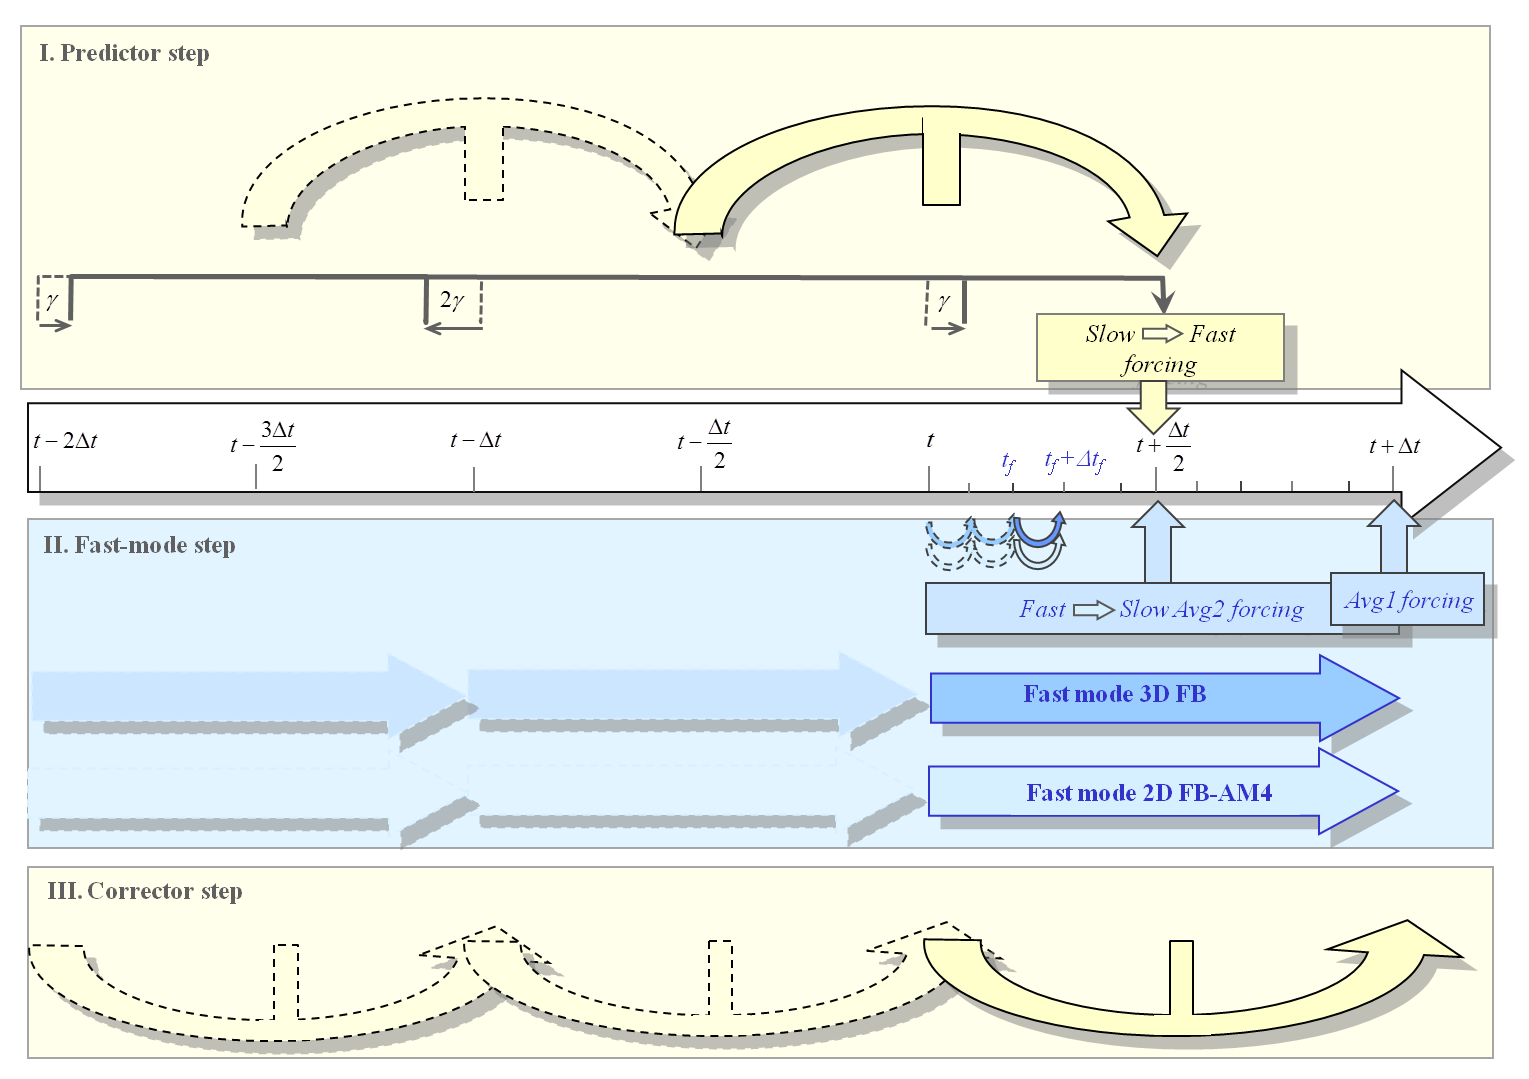
\includegraphics[width=1\linewidth]{CHAP2/Model_TS.png}
		\caption{}
	\end{subfigure}
\caption{ \textit{time-splitting and time-stepping of CROCO model with its non-hydrostatic, compressible (NBQ) kernel. Yellow (blue) background color: slow (fast) kernel. }}
	\label{ModelTS}
\end{figure}
%
\begin{table}
\begin{subequations}
\label{TimeSplit}
\begin{alignat}{3}
 \displaystyle
 %%%%%%%%%%%%%%%%%%%%%%%%%%%%%%%%%%%%%%%%%%%%%%%%%%%%%%%%%%%%%
 &\nonumber \textbf{I.a Time-interpolation: } t_s-\Delta t_s/2\\[0mm]
 %%%%%%%%%%%%%%%%%%%%%%%%%%%%%%%%%%%%%%%%%%%%%%%%%%%%%%%%%%%%%
 \label{TimeSplitIa1}
 &\enspace[\Theta] ^{n-\frac{1}{2}}=\alpha_{n-1}\Theta_s^{n-1}
 +\alpha_{n}\Theta_s^{n}\\[3mm]
 %%%%%%%%%%%%%%%%%%%%%%%%%%%%%%%%%%%%%%%%%%%%%%%%%%%%%%%%%%%%%
 &\nonumber \textbf{I.b Predictor step: } t_s+\Delta t_s/2\\[0mm]
 %%%%%%%%%%%%%%%%%%%%%%%%%%%%%%%%%%%%%%%%%%%%%%%%%%%%%%%%%%%%%
 \label{TimeSplitIb1}
 &\enspace\rho h\mathbf{v}_s^{n+\frac{1}{2}}=
 \rho h\mathbf{v}_s^{n-\frac{1}{2}}
 +\Delta t_s\left(\Lambda_{s,v}^{n}+<\Lambda_{f,v}>^n\right)\\[3mm]
 %
 \label{TimeSplitIb2}
 &\enspace\rho h(\theta_s,\ S_s)^{n+\frac{1}{2}}=
 \rho h(\theta_s,\ S_s)^{n-\frac{1}{2}}
 +\Delta t_s\Lambda_{s,(\theta,S)}^{n}\\[3mm]
 %
 \label{TimeSplitIb3}
 &\enspace\rho_s^{n+\frac{1}{2}}=\rho_{eos}\left(\theta_s^{n+\frac{1}{2}},\ S_s^{n+\frac{1}{2}},\ z_s^{n+\frac{1}{2}}\right)\\[3mm]
 %
 \label{TimeSplitIb4}
 &\enspace\partial_s\rho\omega_s^{n+\frac{1}{2}}=-\partial_t\rho h_s^{n+\frac{1}{2}}
 +\mathbf{\nabla}\cdot\rho h \mathbf{u}_s^{n+\frac{1}{2}}\\[3mm]
 %%%%%%%%%%%%%%%%%%%%%%%%%%%%%%%%%%%%%%%%%%%%%%%%%%%%%%%%%%%%%
 &\nonumber \textbf{I.c AB3-extrapolation: } t_s+\Delta t_s/2\\[0mm]
 %%%%%%%%%%%%%%%%%%%%%%%%%%%%%%%%%%%%%%%%%%%%%%%%%%%%%%%%%%%%%
 \label{TimeSplitIc1}
 &\enspace[[\Psi_s]]^{n+\frac{1}{2}}=
  \beta_{n-2}\Psi_s^{n-2}
 +\beta_{n-1}\Psi_s^{n-1}
 +\beta_{n}\Psi_s^{n}\\[2mm]
 %%%%%%%%%%%%%%%%%%%%%%%%%%%%%%%%%%%%%%%%%%%%%%%%%%%%%%%%%%%%%
 &\nonumber \textbf{II. Fast-mode steps: } t_f\in(t_s,\ t_s+\Delta t_s] \textit{ or } m\in[0,\ N_f)_\mathcal{N}\\[2mm]
 %%%%%%%%%%%%%%%%%%%%%%%%%%%%%%%%%%%%%%%%%%%%%%%%%%%%%%%%%%%%%
 \label{TimeSplitIIa}
 &\enspace\zeta_f^{m+1}=\zeta_f^{m}+\Delta t_f\left(
  w_{surf}^{m}-\mathbf{u}_{surf}^{m}.\mathbf{\nabla}\zeta^{m}\right)\\[2mm]
 %
 \label{TimeSplitIIb}
 &\enspace\rho h u_f^{m+1}=
 \rho h u_f^{m}
 +\Delta t_f\left(
  [[\Lambda_{s,u}]]^{n+\frac{1}{2}}
 -[[\overline{\Lambda_{s,u}}]]^{n+\frac{1}{2}}
 +\Lambda_{f,u}^{m}
% +\overline{\overline{\Lambda_{f,u}}}^{\ m}
 +\overline{\overline{\Lambda_{f,u}}}^{\ m}
 +\overline{\overline{\Lambda_{f,-\mathbf{\nabla}\zeta}}}^{\ m+1}
 \right)\\[2mm]
 %
 \label{TimeSplitIIc}
 &\enspace\overline{\overline{\rho h U}}_f^{\ m+1}=
 \overline{\overline{\rho h U}}_f^{\ m}
 +\Delta t_f\left(
 %[[\overline{\Lambda_{s,u}}]]^{n+\frac{1}{2}}+
 \overline{\Lambda_{f,u}^{m}}
 +\overline{\overline{\Lambda_{f,u}}}^{\ m}
 +\overline{\overline{\Lambda_{f,-\mathbf{\nabla}\zeta}}}^{\ m+1}
 \right)\\[0mm]
 %
 \label{TimeSplitIId}
 &\enspace\rho h w_f^{m+1}=
 \rho h w_f^{m}
 +\Delta t_f\left([[\Lambda_{s,w}]]^{n+\frac{1}{2}}
 +\Lambda_{f,w}^{m+1*}\right)\\[2mm]
 %
 \label{TimeSplitIIe}
 &\enspace\rho h_f^{m+1}=\rho h_f^{m}
 -\Delta t_f\left(
 [[\partial_t\rho h_s]]^{n+\frac{1}{2}}
 +\mathbf{\nabla}\cdot\{\rho h \mathbf{v}\}_f^{m+1}
 \right)\\[0mm]
 %
 \label{TimeSplitIIh}
 &\enspace m=N_f-1:\ \bar{\rho}\zeta_s^{n+1}
 =\bar{\rho}(H+\zeta_f)^{m}
 -\bar{\rho}H_s^{m+1}
 -\Delta t_f\mathbf{\nabla}\cdot\overline{\overline{\rho h\mathbf{u}}}^{\ m+1}\\[2mm]
 %
 \label{TimeSplitIIg}
 &\enspace \textit{Update\ grid:}\ \rho h_f^{m+1},\ z_f^{m+1}\\[2mm]
 %
 %%%%%%%%%%%%%%%%%%%%%%%%%%%%%%%%%%%%%%%%%%%%%%%%%%%%%%%%%%%%%
 &\nonumber \textbf{III.a Filtering: } t_s+\Delta t_s\ \textit{and}\ t_s+\Delta t_s/2\\[0mm]
 %%%%%%%%%%%%%%%%%%%%%%%%%%%%%%%%%%%%%%%%%%%%%%%%%%%%%%%%%%%%%
 \label{TimeSplitIIIa1}
 &\enspace<\Phi_f>^{n+1}=\Phi_f^{m=n+1}\\[0mm]
 \label{TimeSplitIIIa2}
 &\enspace\ll\Phi_f\gg^{n+\frac{1}{2}}=\frac{1}{N_f}\sum_{m=1}^{N_f}\Phi_f^{m}\\[2mm]
 %%%%%%%%%%%%%%%%%%%%%%%%%%%%%%%%%%%%%%%%%%%%%%%%%%%%%%%%%%%%%
 &\nonumber \textbf{III.b Corrector step: } t_s+\Delta t_s\\[0mm]
 %%%%%%%%%%%%%%%%%%%%%%%%%%%%%%%%%%%%%%%%%%%%%%%%%%%%%%%%%%%%%
 %
 \label{TimeSplitIIIb1}
 &\enspace\rho h\mathbf{v}_s^{n+1}=
 \rho h\mathbf{v}_s^{n}
 +\Delta t_s\left(\Lambda_s^{n+\frac{1}{2}*}
 +\ll\Lambda_f\gg^{n+\frac{1}{2}}\right)\\[0mm]
 %
 \label{TimeSplitIIIb2}
 &\enspace\partial_s\rho\omega_s^{n+1}=
 -\partial_{t\ }\rho h_s^{n+1}
 +\mathbf{\nabla}\cdot\rho h \mathbf{u}_s^{\ n+1}
 -\overline{\mathbf{\nabla}\cdot\rho h \mathbf{u}_s}^{\ n+1}
 -\overline{<\mathbf{\nabla}\cdot\rho h \mathbf{u}_s>}^{\ n+1}\\[2mm]
 %
 \label{TimeSplitIIIb3}
 &\enspace\rho h(\theta_s,\ S_s)^{n+1}=
 \rho h(\theta_s,\ S_s)^{n}
 +\Delta t_s\Lambda_{s,(\theta,S)}^{n+\frac{1}{2}*}\\[0mm]
 %
 \label{TimeSplitIIIb4}
 &\enspace\rho_s^{n+1}=\rho_{eos}\left(\theta_s^{n+1},\ S_s^{n+1},\ z_s^{n+1}\right)\\[0mm]
 %
 \label{TimeSplitIIIb5}
 &\enspace\rho h\mathbf{u}_s^{n+1}=\rho h\mathbf{u}_s^{n+1}
 -\overline{\rho h\mathbf{u}_s}^{\ n+1}
 +\overline{\rho h\mathbf{u}_f}^{\ m=N_f-1}
 %%%%%%%%%%%%%%%%%%%%%%%%%%%%%%%%%%%%%%%%%%%%%%%%%%%%%%%%%%%%%
\end{alignat}
\end{subequations}
\end{table}
Predictor (I), fast-kernel Forward-Backward (II) and Corrector (III) steps are shown in horizontal color bands on figure \ref{ModelTS} (yellow for the slow kernel, blue for the fast kernel). After time-interpolating slow-kernel variables to $t_s-\Delta t_s/2$ (step I.a, notation $[.]$), the slow kernel is advanced from $t_s-\Delta t_s/2$ to $t_s+\Delta t_s/2$ with a centered, leap-frog-like, time-stepping (step I.b). Then, to prepare the integration of the fast kernel, the slow-kernel RHS is extrapolated to $t_s+\Delta t_s/2$ based on an AB3 scheme using its previous evaluations at $t_s-2\Delta t_s$, $t_s-\Delta t_s$ and $t_s$ (step I.c, notation $[[.]]$). The fast kernel can in turn be advanced from $t_s$ to $t_s+\Delta t_s$ using a forward-backward like time-stepping (step II) with time-step $\Delta t_f$ satisfying  $N_f=\Delta t_s/\Delta t_f\in\mathcal{N}$. The vertical momentum equation can optionaly be integrated with semi-implicit scheme over the vertical direction.\\ 
The vertical grid is updated at each fast time-step \ref{TimeSplitIIg} but slow-kernel components of the RHS remain constant during the fast-kernel integration. At the last fast time-step, surface elevation displacement for the slow kernel can be recomputed to ensure perfect numerical coherence between the surface kinematic relation and depth-integrated mass conservation (\noparref{TimeSplitIIa} and \noparref{TimeSplitIIh}).\\
Further numerical details such as the values of the interpolation $(\alpha_n)$ or extrapolation $(\beta_n)$ coefficients, the expressions of the slow-kernel RHS terms $(\Lambda_s)$, the expressions of the fast-kernel surface-related pressure force terms $(\Lambda_{f,-\nabla\zeta})$,  the fast-kernel RHS remaining terms $(\Lambda_{f})$ or the implicit fast and slow-kernel RHS terms (indicated by an asterisk) can be found in CROCO dedicated manuals and publications.\\  
%The barotropic-like, depth-independent component is also integrated with the same time-step $\Delta t_f$ with a forward-backward scheme as in \cite{shchepetkin_regional_2005}. 
A major difference with the hydrostatic time-splitting is that the surface elevation displacement is given by the kinematic condition \ref{TimeSplitIIa} and not by the depth-integral of the mass conservation equation. Once the fast-kernel RHS and variables have been filtered both at $t_s+\Delta t_s$ and $t_s+\Delta t_s/2$ (step III.a, notations $<.>$ and $\ll.\gg$), the slow kernel is finally advanced from $t$ to  $t_s+\Delta t_s$ during the leap-frog-like Corrector step (III.b). A star following the time-index superscript indicates the use of an implicit numerical schemes.

Note that the 2D depth-averaged, barotropic-like, horizontal momentum equations (double over-bar notation) \ref{TimeSplitIIc} are advanced in the same way as in \cite{shchepetkin_regional_2005}. The result of this 2D integration is indeed used to correct both the horizontal momentum itself and the RHS of the horizontal momentum equation at Corrector step. It can also be used to require a perfect coherence of the surface elevation displacement and the depth-average transport (at machine precision) during the slow-mode integration.

\color{blue}
\section{Conclusion, discussion of the \textit{ocean model}}
In the present chapter, we proposed a rigorous framework (an "map") for our exploration of ocean \textit{fine scales} in \textit{Terra Incognita}. An analytical, terrain-following s-coordinate model for the conservation of mass, momentum, heat and tracers has first been proposed under general assumptions of a compressible, free-surface ocean (\S \noparref{section_prim_eq}). \\
%An original derivation (to our knowledge) of the evolution of the potential energy of a free-surface column of fluid has been carried out.\\%FA%
We then considered the numerical implementation of this general \textit{ocean model} (\S \noparref{section_croco}). After a consideration of the space-time scales potentially involved in the fine scale ocean dynamics, an original time-splitting has been detailed as an extension of \cite{shchepetkin_regional_2005}'s barotropic/baroclinic time-splitting. It is also a restriction to a two-mode time-splitting of \cite{Auclair2018}'s three-mode time-splitting. This time-splitting allows the integration of both acoustic and surface-induced processes with a smaller time-step in order to make the integration of a compressible, free-surface realistic ocean affordable. It is based on the spectral gaps identified in \ref{velocityscales} between acoustic, surface and internal processes.\\
The region of Gibraltar strait has been chosen as the region of demonstration for its fine-scale dynamics. As a consequence, the LES configurations presented in chapters \ref{chapGBR2D}, \ref{chapGBR3D} and \ref{chapBPE} are not only based on the resulting two-mode CROCO kernel but these configurations have thus been part of the development process itself. 
%The investigation of mixing in real-ocean conditions proposed in chapter \ref{chapBPE} takes roots in the general evolution equation of potential energy proposed in (\S \noparref{section_prim_eq}).
\color{black}
%%%%%%%%%%%%%%%%%%%%%%%%%%%%%%%%%%%%%%%%%%%%%%%%%%%%%%%%%%%%%%%%%%%%%%%%%%%
%%%%%%%%%%%%%%%%%%%%%%%%%%%%%%%%%%%%%%%%%%%%%%%%%%%%%%%%%%%%%%%%%%%%%%%%%%%
%%%%%%%%%%%%%%%%%%%%%%%%%%%%%%%%%%%%%%%%%%%%%%%%%%%%%%%%%%%%%%%%%%%%%%%%%%%
\section{Appendices to the \textit{ocean model}}
\label{annexe_ocmod}
%%%%%%%%%%%%%%%%%%%%%%%%%%%%%%%%%%%%%%%%%%%%%%%%%%%%%%%%%%%%%%%%%%%%%%%%%%%
%%%%%%%%%%%%%%%%%%%%%%%%%%%%%%%%%%%%%%%%%%%%%%%%%%%%%%%%%%%%%%%%%%%%%%%%%%%
%%%%%%%%%%%%%%%%%%%%%%%%%%%%%%%%%%%%%%%%%%%%%%%%%%%%%%%%%%%%%%%%%%%%%%%%%%%

\subsection{$s$-coordinate transformation}
\label{section_annexe2}
The present appendix gathers several formula and relations essential to the development of the numerical implementation of the \textit{ocean model}.
%
%%%%%%%%%%%%%%%%%%%%%%%%%%%%%%%%%%%%%%%%%%%%%%%%%%%%%%%%%%%%%%%%%%%%%%%%%%%%%
\subsubsection{Transformation matrices}
\label{annexe_coordS}
%%%%%%%%%%%%%%%%%%%%%%%%%%%%%%%%%%%%%%%%%%%%%%%%%%%%%%%%%%%%%%%%%%%%%%%%%%%%%
The transformation matrix of the generalized coordinate transformation is:
\begin{equation}
    \displaystyle
    \Lambda^z_s=
    \begin{pmatrix}
    1 & 0 & 0 & 0 \\
    0 & 1 & 0 & 0 \\
    0 & 0 & 1 & 0 \\
    \frac{\partial z}{\partial t} & \frac{\partial z}{\partial x}
    & \frac{\partial z}{\partial y} & h=\frac{\partial z}{\partial s}
    \end{pmatrix}
\end{equation}
and the inverse transformation is given by:
\begin{equation}
    \displaystyle
    \Lambda_z^s=
    \begin{pmatrix}
    1 & 0 & 0 & 0 \\
    0 & 1 & 0 & 0 \\
    0 & 0 & 1 & 0 \\
    \frac{\partial s}{\partial t} & \frac{\partial s}{\partial x}
    & \frac{\partial s}{\partial y} & \frac{\partial s}{\partial z}
    \end{pmatrix}
\end{equation}
The Jacobian of the transformation $J=det(\Lambda^z_s)$ is the (specific) thickness:
\begin{equation}
 \displaystyle
 J=h=\frac{\partial z}{\partial s}=\frac{\partial z}{\partial s}\bigg\vert_{xyt}
\end{equation}
\cite{griffies_fundamentals_2004} further define the infinitesimal  thickness for modelling developments:
\begin{equation}
 \displaystyle
 \delta h=\frac{\partial z}{\partial s} \delta s
\end{equation}

%%%%%%%%%%%%%%%%%%%%%%%%%%%%%%%%%%%%%%%%%%%%%%%%%%%%%%%%%%%%%%%%%%%%%%%%%%%%%
\subsubsection{Formula and identities}
%%%%%%%%%%%%%%%%%%%%%%%%%%%%%%%%%%%%%%%%%%%%%%%%%%%%%%%%%%%%%%%%%%%%%%%%%%%%%
Base on the transformation matrices, the $s$-coordinate transformations can be rewritten:
\begin{subequations}
  \begin{alignat}{2}
  \displaystyle 
  &\frac{\partial A}{\partial t}\bigg\rvert_{xz} &&=
   \frac{\partial A}{\partial t}\bigg\rvert_{xs}
  - \frac{1}{h} \frac{\partial A}{\partial s}\bigg\rvert_{tx}
  \frac{\partial z}{\partial t}\bigg\rvert_{xs}\\[4mm]
  &\frac{\partial A}{\partial x}\bigg\rvert_{tz} &&=
   \frac{\partial A}{\partial x}\bigg\rvert_{ts}
  - \frac{1}{h} \frac{\partial A}{\partial s}\bigg\rvert_{tx}
  \frac{\partial z}{\partial x}\bigg\rvert_{ts}\\[4mm]
  &\frac{\partial A}{\partial z}\bigg\rvert_{tx} &&=
   \frac{1}{h}
   \frac{\partial A}{\partial s}\bigg\rvert_{tx}
  \end{alignat}
\end{subequations}
whereas material derivatives satisfy:
\begin{subequations}
  \begin{alignat}{2}
  \displaystyle 
  & \frac{d}{dt} &&=\frac{\partial}{\partial t}\bigg\vert_z
  + \mathbf{u}.\mathbf{\nabla}_z
  + w\frac{\partial }{\partial z}\\[4mm]
  & &&=\frac{\partial}{\partial t}\bigg\vert_s
  + \mathbf{u}.\mathbf{\nabla}_s
  + \dot{s}\frac{\partial}{\partial s}
  \end{alignat}
\end{subequations}
This leads to:
\begin{equation}
  \displaystyle 
  \dot{z} =\frac{dz}{dt}\bigg\vert_s=\frac{\partial z}{\partial t}\bigg\vert_s
  + \mathbf{u}.\mathbf{\nabla}_s z
  + \dot{s}\frac{\partial z}{\partial s},\quad r\quad
  \dot{s} =\frac{ds}{dt}\bigg\vert_z=\frac{\partial s}{\partial t}\bigg\vert_z
  + \mathbf{u}.\mathbf{\nabla}_z s
  + w\frac{\partial s}{\partial z}
\end{equation}
Using the identities:
\begin{equation}
  \displaystyle
  \frac{\partial s}{\partial t}\bigg\vert_z =
  \left(\frac{\partial t}{\partial s}\bigg\vert_z\right)^{-1},\quad
  \frac{\partial s}{\partial x}\bigg\vert_z =
  \left(\frac{\partial x}{\partial s}\bigg\vert_z\right)^{-1},\quad
  \frac{\partial s}{\partial y}\bigg\vert_z =
  \left(\frac{\partial y}{\partial s}\bigg\vert_z\right)^{-1},\quad
  \frac{\partial s}{\partial z}\bigg\vert_x =
  \left(\frac{\partial z}{\partial s}\bigg\vert_x\right)^{-1
\end{equation}
several relations can be obtained from the triple product rule and the coordinate transformations are given by:
\begin{equation}
  \displaystyle
  \frac{\partial z}{\partial t}\bigg\vert_s =
  -\frac{\partial s}{\partial t}\bigg\vert_z\frac{\partial z}{\partial s}\bigg\vert_s,\quad
  \frac{\partial z}{\partial x}\bigg\vert_s =
  -\frac{\partial s}{\partial x}\bigg\vert_z\frac{\partial z}{\partial s}\bigg\vert_s,\quad
  \frac{\partial z}{\partial y}\bigg\vert_s =
  -\frac{\partial s}{\partial y}\bigg\vert_z\frac{\partial z}{\partial s}\bigg\vert_s\\
\end{equation}

%%%%%%%%%%%%%%%%%%%%%%%%%%%%%%%%%%%%%%%%%%%%%%%%%%%%%%%%%%%%%%%%%%%%%%%%%%%%%
\subsubsection{Local orthonormal coordinates}
%%%%%%%%%%%%%%%%%%%%%%%%%%%%%%%%%%%%%%%%%%%%%%%%%%%%%%%%%%%%%%%%%%%%%%%%%%%%%
\cite{griffies_fundamentals_2004} further defines in his chapter (6.4) a system of orthonormal coordinates:
\begin{equation}
  \displaystyle 
  \mathbf{e}_{x^*} =\frac{\mathbf{y}\wedge{\mathbf{\nabla}s}}
  {\norm{\mathbf{y}\wedge{\mathbf{\nabla}s}}},\quad
  \mathbf{e}_{y^*} =\mathbf{e}_s\wedge{\mathbf{e}_{x^*}},\quad
  \mathbf{e}_s =\frac{\mathbf{\nabla}s}{\norm{\mathbf{\nabla}s}}
\end{equation}
In this particular case ($\mathbf{e}_s.\mathbf{z}$) has a unique sign, the basis vectors can be rewritten:
\begin{equation}
  \displaystyle 
  \mathbf{e}_{x^*} =\frac{\mathbf{x}+S_x\mathbf{z}}{\sqrt{1+S_x^2}},\quad
  \mathbf{e}_{y^*} =\frac{-S_xS_y\mathbf{x}+(1+S_x^2)\mathbf{y}+S_y\mathbf{z}}{\sqrt{1+S^2)(1+S_x^2)}},\quad
  \mathbf{e}_s =\frac{(-\mathbf{S},1)}{\sqrt{1+S^2}}
\end{equation}
The s-coordinate transformation is a rotation and:
\begin{equation}
   \displaystyle
   \mathbf{e}_{x^*y^*s}=\Lambda_{s}^{z}\mathbf{e}_{xyz}
\end{equation}
Note in particular the definition of the slope $\mathbf{S}$ and its norm $S=\norm{\mathbf{S}}$ used to rewrite the orthonormal basis:
\begin{equation}
   \displaystyle
   \mathbf{S}=\mathbf{\nabla}_s z=
   -\frac{\partial z}{\partial s}\mathbf{\nabla}_z s=\left( S_x,\ S_y,\ 0 \right)
\end{equation}
where $\mathbf{\nabla}_s z$ is "the horizontal gradient of the height of a fluid parcel as taken along surfaces of constant generalized vertical coordinate s" \citep{griffies_fundamentals_2004}.

Note that this orthonormal basis is not used to project the equations of the model. S-coordinates are "only" used as a change of variable whereas equations and vector quantities remain written in the original Cartesian or spherical basis. The present s-coordinate orthonormal basis is presented here to be latter used in the computation of fluxes through s-surfaces.


%%%%%%%%%%%%%%%%%%%%%%%%%%%%%%%%%%%%%%%%%%%%%%%%%%%%%%%%%%%%%%%%%%%%%%%%%%%%%
\subsection{Operators \& relations in s-coordinates}
\label{annexe_s-coord}
%%%%%%%%%%%%%%%%%%%%%%%%%%%%%%%%%%%%%%%%%%%%%%%%%%%%%%%%%%%%%%%%%%%%%%%%%%%%%

%%%%%%%%%%%%%%%%%%%%%%%%%%%%%%%%%%%%%%%%%%%%%%%%%%%%%%%%%%%%%%%%%%%%%%%%%%%%%
\subsubsection{Divergence of the velocity field in s-coordinates}
%%%%%%%%%%%%%%%%%%%%%%%%%%%%%%%%%%%%%%%%%%%%%%%%%%%%%%%%%%%%%%%%%%%%%%%%%%%%%
Using :
\begin{equation}
 \displaystyle
 \frac{\partial}{\partial t} \frac{\partial z}{\partial s}\bigg\vert_{tx}= \frac{\partial h}{\partial t} \qquad and \qquad \frac{\partial}{\partial x} \frac{\partial z}{\partial s}\bigg\vert_{tx}= \frac{\partial h}{\partial x}
\end{equation}
%and
%\begin{equation}
% \displaystyle
% \frac{\partial}{\partial x} \frac{\partial z}{\partial s}\bigg\vert_{tx}= \frac{\partial h}{\partial x}
%\end{equation}
%
the expression of the divergence of the velocity field in s-coordinates can be written:
\begin{subequations}
  \begin{alignat}{2}
  & h \ \mathbf{\nabla}.( \mathbf v) &&= h \frac{\partial u}{\partial x} \bigg \rvert_{zt} +h \frac{\partial v_z}{\partial z} \bigg \rvert_{xt}\\[4mm]
  & && = h \frac{\partial u}{\partial x} \bigg \rvert_{st} - \frac{h}{h} \frac{\partial u}{\partial s}\bigg \rvert_{tx} \frac{\partial z}{\partial x}\bigg \rvert_{ts}
  \quad + \frac{h}{h}  \frac{\partial}{\partial s} \bigg ( v_s + \frac{\partial z }{\partial t}\bigg \rvert_{xs} + u \frac{\partial z}{\partial x}\bigg \rvert_{ts} \bigg )\\[4mm]
  & && = h \frac{\partial u}{\partial x} \bigg \rvert_{st} -  \frac{\partial u}{\partial s}\bigg \rvert_{tx} \frac{\partial z}{\partial x}\bigg \rvert_{ts} 
  \quad +  \frac{\partial v_s}{\partial s} +  \frac{\partial h}{\partial t} + u \frac{\partial h}{\partial x} + \frac{\partial u}{\partial s}\bigg \rvert_{tx} \frac{\partial z}{\partial x}\bigg \rvert_{ts}\\[4mm]
  & && = \frac{\partial v_s}{\partial s}\bigg \rvert_{tx} + \frac{\partial h u}{\partial x} \bigg \rvert_{ts}+ \frac{\partial h}{\partial t}\bigg \rvert_{xs}
  \end{alignat}
\end{subequations}
Note that this is a particular case of the formulation of a change of variables with its Jacobian ($J=h$ in the present case). %This leads to several useful conservative formulations in the following section.
%
%%%%%%%%%%%%%%%%%%%%%%%%%%%%%%%%%%%%%%%%%%%%%%%%%%%%%%%%%%%%%%%%%%%%%%%%%%%%%
\subsubsection{Conservative "flux" forms: kinematics \& dynamics}
%%%%%%%%%%%%%%%%%%%%%%%%%%%%%%%%%%%%%%%%%%%%%%%%%%%%%%%%%%%%%%%%%%%%%%%%%%%%%
Two general conservative formulations can be obtained combining this with the continuity equation \citep{auclair_woceanfr_2011}\footnote{WOcean.fr Web Site: \url{http://poc.omp.obs-mip.fr/auclair/WOcean.fr/SNH/Restricted/NH-NBQ/Sources/Images/png/Coord_demo.png}\label{WOcean_scoord}}.

$A$ is a property given per unit mass (thermodynamically intensive) (see the demonstration on web site). The first two (conservative) relations are fundamentals to analytical and numerical modeling.


\textbf{\textit{Based on the conservation of mass:}}
\begin{equation}
  \displaystyle 
  \rho \frac{d A}{dt}
  =\frac{\partial \rho A}{\partial t}\bigg\rvert_{xz}
  +\frac{\partial \rho A u}{\partial x}\bigg\rvert_{tz}
  +\frac{\partial \rho  v_s}{\partial z}\bigg\rvert_{tx}
\end{equation}

\textbf{\textit{Based on the conservation of mass \& in s-coordinates:}}
\begin{equation}
  \displaystyle 
  \rho h \frac{d A}{dt}
  =\frac{\partial \rho h A}{\partial t}\bigg\rvert_{xs}
  +\frac{\partial \rho h A u}{\partial x}\bigg\rvert_{ts}
  +\frac{\partial \rho  A v_s}{\partial s}\bigg\rvert_{tx}
\end{equation}
\textbf{\textit{A kinematic, non-conservative formulation}} can be obtained without the continuity equation:
\begin{equation}
\frac{d A}{d t} = \frac{\partial A}{\partial t} \bigg\rvert_{xs} + u \frac{\partial A}{\partial x} \bigg\rvert_{ts} + \frac{v_s}{h}\frac{\partial A}{\partial s}\bigg\rvert_{tx}
\end{equation}
The demonstration is given in \citep{auclair_woceanfr_2011}$^{\noparref{WOcean_scoord}}$.\\

\textbf{\textit{Conservation of mass:}}
note finally that the conservation of mass $A=1$ can then be rewritten:
\begin{equation}
  \displaystyle 
  \label{mass_s}
  h\frac{d\rho}{d t}
  =\frac{\partial \rho h }{\partial t}\bigg\rvert_{xs}
  +\frac{\partial \rho h u}{\partial x}\bigg\rvert_{ts}
  +\frac{\partial \rho  v_s}{\partial s}\bigg\rvert_{tx}
\end{equation}

Additionnally, the evolution of $\rho$ in equation \ref{eq_diff_cart} can be rewritten in s-coordinates as:
\begin{equation}
\label{eq_diff_s}
\displaystyle
h \frac{d \rho }{d t} \approx
\frac{\partial}{\partial x} \bigg(h \kappa^h \frac{\partial \rho}{\partial x}\bigg\rvert_{ts}\bigg)_{ts}
+ \frac{\partial}{\partial s} \bigg(\frac{\kappa^v}{h} \frac{\partial \rho}{\partial s}\bigg\rvert_{tx}\bigg)_{tx} 
\end{equation}
with: $\kappa_c^h \approx \kappa^h$ and $\kappa_c^v \approx \kappa^v$.\\




%\noindent\textit{Quantification du mélange diapycnale : évolution de la BPE}\\
%L'énergie potentielle de "background", i.e. non-disponible, ou BPE (pour \textit{Background Potential Energy}), d'un volume de fluide est l'énergie potentielle minimale obtenue après ré-arrangement adiabatique des parcelles de fluide du volume \citep{winters_2013}. De nombreuses études se sont attachées à relier l'évolution de cette énergie "non disponible" (notée ci-dessous $E_b$) consécutive au mélange diapycnal dans un domaine fermé, la réalisation d'un bilan rigoureux de cette forme d'énergie potentielle dans une région océanique pour laquelle la position de la surface libre varie est une contribution originale du LAERO développée dans le cadre des travaux de thèse de Margaux Hilt et appliquée dans le cadre du présent "Courants de Gravité". Son équation d'évolution en coordonnées verticales "s" est ainsi donnée par:
%\begin{subequations}
%  \begin{alignat}{2}
%  \displaystyle
% &\frac{d E_b}{d t} &&= \quad g\int_x \int_{-1}^0 \rho h \frac{\partial z^*}{\partial t}\bigg\rvert_{xs} \ dx ds\\
% & &&\quad +g\int_x \int_{-1}^0\rho v_s \frac{\partial z^*}{\partial s}\bigg\rvert_{tx} \ dx ds
%+g\int_x \int_{-1}^0 \rho h u \frac{\partial z^*}{\partial x}\bigg\rvert_{ts} \ dx ds \\
% & && \quad - g\bigg[ \int_{-1}^0 \rho h z^* u \ ds\bigg]_{x} - g\bigg[ \int_x\rho z^* v_s \ dx\bigg]_0^1 \\
% & && \quad + g\bigg[ \int_{-1}^0 h z^* \kappa^h \frac{\partial \rho}{\partial x}\bigg\rvert_{ts} \ ds \bigg]_{x}
% - g\int_x \int_{-1}^0 h \kappa^h \frac{d z^*}{d \rho} \frac{\partial \rho}{\partial x}\bigg\rvert_{ts}^2 \ dx ds \\
% & && \quad + g\bigg[ \int_x z^* \frac{\kappa^v}{h} \frac{\partial \rho}{\partial s}\bigg\rvert_{tx} \ dx \bigg]_0^1
% - g\int_x \int_{-1}^0 \frac{\kappa^v}{h} \frac{d z^*}{d \rho} \frac{\partial \rho}{\partial s}\bigg\rvert_{tx}^2 \ dx ds
%\end{alignat}
%\end{subequations}
%où $z^*$ est la position d'une particule fluide après ré-arrangement adiabatique du champ de masse, $\rho$ est la masse volumique, $u$ et $v_s$ sont respectivement les vitesses horizontales et verticales en coordonnées "s", $g$ est l'accélération de la pesanteur, $h$ est la hauteur de la colonne d'eau et $\kappa^h$ et $\kappa^v$ sont les diffusités horizontales et verticales. $s=0$ en surface et $s=-1$ au fond.
%Les derniers termes du membre de droite sont en particulier des sources de BPE dues au mélange diapycnal et font intervenir dans la forme de cette équation un coefficient de diffusion. C'est ce coefficient qui permet de quantifier le mélange diapycnal car il est le résultat de tous les mécanismes irréversibles de diffusion. Dans le cas de simulations numériques, il va inclure en plus de la dissipation moléculaire explicite, la dissipation implicite induite par les schémas à différence finie. Il prendra aussi en compte la paramétrisation du mélange dans les simulations de type RANS ou LES lors d'évènements de mélange.

%L'évaluation de la BPE et de son évolution a pour finalité d'être appliqué dans des cas de simulation réaliste de l'océan mais est aussi applicable à la simulation physique.\\


%\hypersetup{pdfborder=0 0 0}
%\vspace{10\baselineskip}


%\selectlanguage{french}


\section{Resume français}




%-------------------------------------------------------------------------------------
\section{Papier 3D}
\subsection{Introduction}

The Atlantic - Mediterranean exchange occurring in the Strait of Gibraltar has been explained summarily in previous part (2D). It consists in Med waters exiting the Strait at depth as what has been dubbed the 'Mediterranean outflow' while Atl waters enter the Mediterranean basin at the surface.

Those Atlantic waters entering at the Strait are the principal contribution to the Mediterranean inflowing water budget, with the average transport of Atl waters at Gib being of the order of 1Sv. The net exchange itself is of the order of 0.1Sv as a positive entry that offsets the otherwise net evaporation occurring on the integrated surface of the Mediterranean basin \citep{bryden_1994}.
Since the Med basin is otherwise a closed basin, the Mediterranean waters exiting the Strait of Gibraltar are the result of the transformations into intermediate and deep water masses of the Atl waters that circulated in the Mediterranean.
More details are provided in this section on the characteristics of the Strait, the exchange and its variability and the processes that take place during it.






\subsubsection{Circulation in neighbouring areas (Cadix and Alboran)}

(de Pascual-Collar ; NAjanro 2012 ; Sanchez Garrido 2013 ;Lorente 2019 ; garcia lafuente 2017)


\textit{Atlantic side}

The surface waters that end up entering the Strait are NACW and SAW\citep{millot_2014,naranjo_2015}. They are carried by the Portugal and Azores Current into Gib as part of the eastern branch of the north atlantic subtropical gyre \citep{barton_2001}

Below this surface circulation, can find in the Northern Atlantic the med outflow/the mediterranean watermass that was transported out of the Strait by the MEditerreanaen outflow. It first flows in the Gulf of Cadix, rotating to north due to geostrophy and flowing along the bathymetry of the continental slope\citep{price_1993,gasser_2017} and west of the Gulf of Cadiz stabilizes to its neutral buoyancy level at 1000m depth as the Mediteranean water mass\citep{price_1993}. Meddies, salty lenses of water with negative (?) vorticity able to 'survive' for years that are encountered in the open ocean, are generated along the canyons and caps encountered by the Mediterranean outflow in the Gulf of Cadiz \citep{bashmachnikov_2015}. The Mediterranean outflow itself participates in the global circulation/north atlantic overturning circulation(?) by salinification of the overall north atlantic basin with the spreading of the mediterranean water mass in the open ocean and decaying of meddies, but also with a part of the outflow directly joining circulation at the pole \citep{price_1993,jia_2007}.


\textit{Mediterranean side}


Surface waters exiting the Strait at the east enter the Alboran Sea as the Atlantic Jet (AJ). The circulation of the Alboran Sea is variable, with the most common state having two anticyclonic gyre (WestarnAlboranGyre ans EasternAlboranGyre), but not uncommon that only one of the two is present \citep{millot_2005}. The WAG is coupled to the Atlantic jet, that usually constitutes its northern branch, however variability of the AJ due to meteorological and tidal forcing can destabilize this system \citep{sanchez-garrido_2013,lorente_2019}.

At depth, several mediterranean water masses enter the strait. In the Alboran Sea, identified are LIW (for Leventine Intermediate Water) and WMDW(West MEditerranean Deep Water), with other water masses of the western med bassin like TDW (Thryenian Deep Water) also being detected (maybe)(Millot). There is a south/north repatition of those watermasses, with TDW, LIW and other intermediate waters more abundant in northern part of Alboran sea, and WMDW flowing more in south part \citep{millot_2014}. As the depth from teh Alboran to the Strait decreases, it is more difficult for the deeper WMDW to enter the strait, and the flow can be regulated by mechanisms such as the strength of the WAG or the overall production of WMDW linked to winter convection (Najanro 2012).


\textit{Gen}

Whether look at inflowing (in reference to the med basin) Atl waters or outflowing (ditto) Med waters, they incorporate signature of respectively the med waters (Macias 2006) and atl waters (Millot 2006,GarciaLafuente2011). This is due to mixing occurring in the Strait, driven by small scale processes of varying strength. 


%%%%%%%%%%%%%%%%%%%%%%%%%%%%%%%%%%%%%%%%%%%%%%%%%%%%%%%%%%%%%%%%%%%%%%%%%%%%
\subsubsection{Morphologie et marée barotrope et masses d'eaux (et ajouter atm???)}
%%%%%%%%%%%%%%%%%%%%%%%%%%%%%%%%%%%%%%%%%%%%%%%%%%%%%%%%%%%%%%%%%%%%%%%%%%%%%


The Strait is inclined of 15$^\text{o}$ from the east direction. Away from continental plateau, Camarinal Sill is the shallowest point with depth averaging at 300m. Relative to Camarinal Sill, Strait is narrower but deeper on the east side. On the west side, shallower, with two troughs on each side of a submarine mount called Majuan Bank. The northern trough is shallower than the southern one, which also includes another sill, called Espartel Sill. Those two troughs are the two pathways the Med outflow take to join the Gulf of Cadix, with most of the flow taking the southern deeper path (18 \% au nord selon Soto-Navarro 2014)


The barotropic M2 semi-durnal tide from the North Atlantic is the foremost varying signal for the currents in the Strait, propagating from south to north with amplitude decreasing from west to east\citep{candela_1990}. During Flood (ebb) tide, barotropic currents ate westward(eastward). The Currents associated with the barotropic tide are same amplitude as the mean circulation, can reverse the flow of med and/or atl waters for certain sections(Sanchez Roman 2012), and have a pronounced neap-spring tide cycle.

Wind is funnelled through the strait and is either westward or eastward/principally zonal with speed can reach 25m/s(Candela 1989). Wind stress affects only the first tens of meters of circulation in the Strait (Candela 1989), which can be sufficient to affect the Atlantic Jet, either accelerating(and making it exit the Strait at various angle) or decelerating it(can even stop it)(Lorente2019). Otherwise, the integrated effect of atmospheric pressure over the Mediterranean basin influence the net flow through the Strait(Garcia Lafuente 2002).





%%%%%%%%%%%%%%%%%%%%%%%%%%%%%%%%
\subsubsection{Baroclinic Exchange and small scale processes}


The circulation of eastward Atlantic waters at the surface and westward Mediterranean waters at depth sets up a baroclinic exchange in the Strait of Gibraltar. Due to amplitude of the barotropic currents, it is intermittent with regard to the M2 tide. One can thus see the exchange as a Reynolds(?) decomposition of an average with tidal contribution as eddy-fluxes that impacts secondary characteristics of the exchange (Naranjo 2014, etc..), and which have a more important amplitude at CS (Vargas2006).  

The exchange varies with other greater timescales than the semi-diurnal tide, with the lower frenquencies (seasonal,interannual) usually linked to atmospheric forcing over the Mediterranean (SanchezRoman2012?). But the tidal eddy-fluxes have their own variability linked to the spring-tide cycle and monthly tide, with for example a greater depth and stronger shear during neap tides, but more intense mixing in spring tide (Naranjo 2014, Vargas 2006).

Behind those characteristics varying at the tidal time-scale are small scale processes occurring in the Strait of Gibraltar.



Firstly, due to the limited horizontal and vertical extent of the Strait that channels the superposed average exchange flow and barotropic tidal currents, the flow in the Strait can become supercritical in regard to internal gravity wave propagation. East (west) of the Camarinal Sill the flow in atl (resp. med) layer will become supercritical, although the detail of how regular/their disposition and geometrical extent depends on the framework one uses. (exemples: Farmi et Armer 1988,Sannino 2007,Sanchez Roman 2012,Vargas 2006...)In particular, hydraulic control occurs at Camarinal Sill episodically.

There, development of two hydraulic jump reflecting the geometry of teh sill and can be observed on satellite imagery (brandt1996).The hydraulic jump stays approximately 4 hours at CS during outflows(Vlasenko 2009) and is where intense mixing occurs (Wesson andGregg;Lafuente...2011,MAcias2006(?)), billows from Kelvin-Helmoltz type instability of the flow in the lee of the hydraulic jump and advected westward by med waters(Wesson andGregg). In addition Bruno 2013, the establishment of hydraulic jump brings chlorophyll-rich waters in the center of the Strait.

Then propagate as LAIWs (Large amplitude Internal waves) also called solitary waves (.Farmer and Armi 1988) due to balance between non-linear and non-hydrostatic dispersion. Have been observed at the surface, and at depth (Ziegenbein (1970), Watson and Robinson 1990,Farmer and Armi 1988,SanchezGarrido 2008,etc.). They transport some chlorophyll (Bruno2013) and expect to make remote mixing in Alboran Sea.

ISW are generated at each tide except when westward current are not strong enough for hydraulic criticality at for neap tide (Watson and Robinson 1990, Garcia Lafuente 2000). Refracted as it exits the Strait by interaction with its boundaries, either as a curve or asymmetrically with an angle in the north(Watson and Robinson 1990).

The hydraulic jump and generation process can be achieved in numerical simulation by hydrostatic models but need non-hydrostatic one for propagation (Brandt 1996 ; (Vlasenko 2009)).



%%%%%%%%%%%%%%%%%%%%%%%%%%%%%%%%%%%%%%%%%%%%%%
\subsubsection{Impact, num et Plan}

Those small scale processes are responsible for the mixing of atl and med waters in the Strait, and the characteristics of the water masses involved in the baroclinic exchange at Gibraltar are not conserved(garcia lafuente 2017 : difficult to link characteristics at ES (INGRES, long term mooring to monitor outflow) to processes in the Mediterranean). The enhanced mixing in the Strait then has to be parametrized in coarsely resolved global/regional models the feedback to/in water mass composition that will impact circulation of the MEditerranean and North Atlantic. 


Following Hilt2020, here 3D sigma model,non-hydrostatic and decadal horizontal resolution that at least resolves the greater scales of mixing in the Strait. In particular focus of different tidal forcing case along a neap-spring tide cycle, how the flow characteristics and intensity of mixing processes is affected in simulation by this variability.


The numerical simulation framework constituted of three simulation periods is presented in section \ref{section3Dnum}, with various diagnosis that have been applied to said simulations /experiments then presented (blah) in section \ref{PartDiag3D} . Section \ref{section3DRes} presents results pertaining to the hydrological state of the flow depending on the strength of barotropic tidal currents, the propagation of ISW in the simulations, then areas of generation of primary instabilities, ending with a comparison of turbulence scheme.






\subsection{Numerical Configuration}
\label{section3Dnum}
\subsubsection{Numerical framework}

Simulations are run using CROCO-NBQ as was the case in Hilt 2020 (see a presentation of CROCO-NBQ there ... and in introduction of manuscript???) . Table \ref{tab_NH-HR} summarize some simulation choice. Otherwise, Non-linear equation of state, noslip condition at the bottom,etc...  The turbulent closure scheme used in all simulations except the ones of paragraph ... is Smagorinsky with coef chosen 0.05. For paragraph ... three simulations use Smago with coefs $10{-3}$,$10{-2}$,$10^{-1}$ , and one use GLSk-$\epsilon$.

Bathymetry data from 100m resolved MNT SHOM, smoothed for pressure gradient... is shown in figure \ref{FigBathy3D}. (bathy seuillée?)


Initialisation and open boundary conditions (that incude tdial forcing) are from a simulation of the operational Med and Black Sea ENEA using MitGCM (ENEA, Rome)\footnote{http://www.enea.it/it/seguici/pubblicazioni/pdf-volumi/cresco-report-2016.pdf}, whch serves as parent simulation. The parent simulation as an horizontal resolution in the strait of $\approx$ 700m and vertical z-levels (repartition?), that are interpolated on grid of horizontal resolution 45 m with 40 evenly spaced vertical $\sigma$-levels. As noted in table ..., this is sufficient to be more resolved in the vertical direction than in the horizontal for the whole simulation domain. At Camarinall Sill, vertical resolution varies from $\approx$7.5m at the top to $\approx$12.5m downslope. No atmospheric forcing is embedded in the simulation.

The first 6 hours of simulation are run in CROCO-Hydro at 50m resolution and the last field is used to restart in NBQ mode. Otherwise the balance in MitGCM is to coarse for stability at high resolution.

\begin{table}[!h]
        \centering
        \begin{tabular}{|p{\linewidth/3}|c|c|}
                \hline
                Grid Extension & \multicolumn{2}{c|} {6°4.8'W  5°3.4'W ;}\\
                & \multicolumn{2}{c|} {35°23.8'N  36°27.4'N}\\
                Number of horizontal grid points & \multicolumn{2}{c|} {2049x2621}  \\
                Number of vertical $\sigma$-levels & \multicolumn{2}{c|} {40} \\
                $\Delta x = \Delta y$ & \multicolumn{2}{c|} {45 m}\\
                Depth & Min & Max\\
                & 26 m & 960 m\\
                $\Delta$z & 0.7 m & 24 m\\
                Internal time-step ($\Delta t_s$) & \multicolumn{2}{c|} {1 s}\\
                External time-step ($\Delta t_f$) & \multicolumn{2}{c|} {1/11 s(change 1/14)}\\
                Advection scheme & \multicolumn{2}{c|} {WENO-5} \\
                Viscosity $\nu$ & \multicolumn{2}{c|} {10$^{-6}$ m$^2$/s} \\
                Diffusivity $K_\rho$(aussi Ks et Kt) & \multicolumn{2}{c|} {10$^{-6}$ m$^2$/s}\\
                Pressure/accoustic wave speed$C_s$ & \multicolumn{2}{c|} {400 m/s}\\
                Tidal harmonics (from ENEA) & \multicolumn{2}{c|} { $\text{M}_{\text{2}}$, $\text{S}_{\text{2}}$,$\text{K}_{\text{1}}$, $\text{O}_{\text{1}}$ }\\
                \hline
        \end{tabular}
        \captionof{table}{Simulation parameters}
        \label{tab_NH-HR}
\end{table}


\begin{table}[!h]
        \centering
        \begin{tabular}{|c|c|}
                \hline
                Closure scheme & Simulation name\\
                \hline
                Smago 0.005 & SimIT,SimNT,SimST\\
                Smago 0.001 & SimIT-S001\\
                Smago 0.01 & SimIT-S01\\
                Smago 0.1 & SimIT-S1\\
                GLS K-$\epsilon$ & SimIT-Kep\\
                \hline
        \end{tabular}
        \captionof{table}{Simulation names (ou combiner avec tableau d'avant ???)}
        \label{tab_sim3Dnames}
\end{table}


\subsubsection{Tidal forcing and simulation period}
The tidal forcing is integrated to the boundary forcing by the parent simulation. As indicated in table \ref{tab_NH-HR},  it comprises four tidal harmonics (?)($\text{M}_{\text{2}}$, $\text{S}_{\text{2}}$, $\text{K}_{\text{1}}$, $\text{O}_{\text{1}}$). Due to computational cost constraints, simulations are run for 3 days along 3 different periods of September of year 2017 (close to equinox). The date of the beginning and end of each NBQ simulation is surmised in table \ref{tab_dates_MIV}, and does not include the 6hour hydrostatic spin up period. The comparison of the sea-level anomaly between a grid point near Tarifa (coord -5.6° - 36.01°) in both the parent MitGCM and CROCO simulation and the tidal gauge data (from Puertos del Estado) are shown in figure \ref{fig_maree_tar}. Can see close to the parent simulation except in the neap tide period.

\begin{table}[h]
        %\begin{minipage}{.6\textwidth}
        \centering
        \begin{tabular}{|c|c|c|}
                \hline
                Situation & Simulation name & Dates (UTC)\\
                \hline
                Intermediate Tide & SimIT & 10/09/2017 19h00 - 13/09/17 01h00  \\
                Neap Tide& SimNT & 13/09/2017 16h00 - 15/09/17 17h00 \\
                %\hline
                Spring Tide& SimST & 19/09/2017 22h00 - 21/09/17 23h00  \\
                \hline
        \end{tabular}
        \captionof{table}{Périodes de simulation pour les 3 sitituations VE, MM et ME}
        \label{tab_dates_MIV}
        %\end{minipage}
\end{table}

\begin{figure}[!h]
        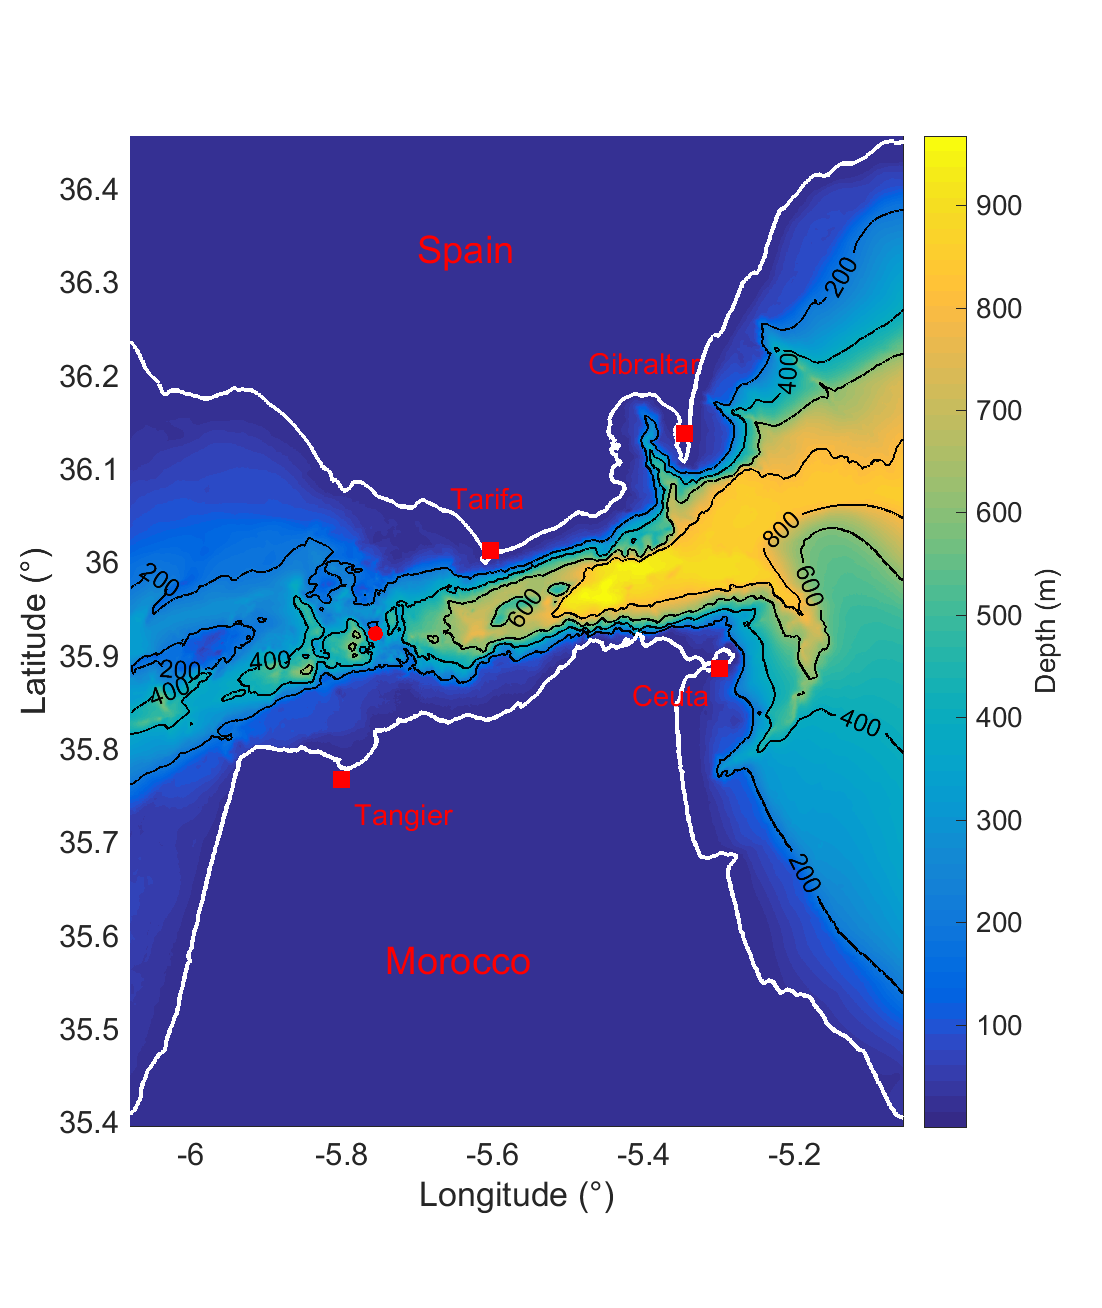
\includegraphics[width=0.5\textwidth]{./GBR3D/FigBathyVHR.png}
        \caption{Area and Bathymetry used for the simulations. The red dot denotes the point at Camarinal Sill where the zonal barotropic current is taken as reference in following figures.!!!Changer en anglais tangIer}
        \label{FigBathy3D}
\end{figure}



\begin{figure}[!h]
        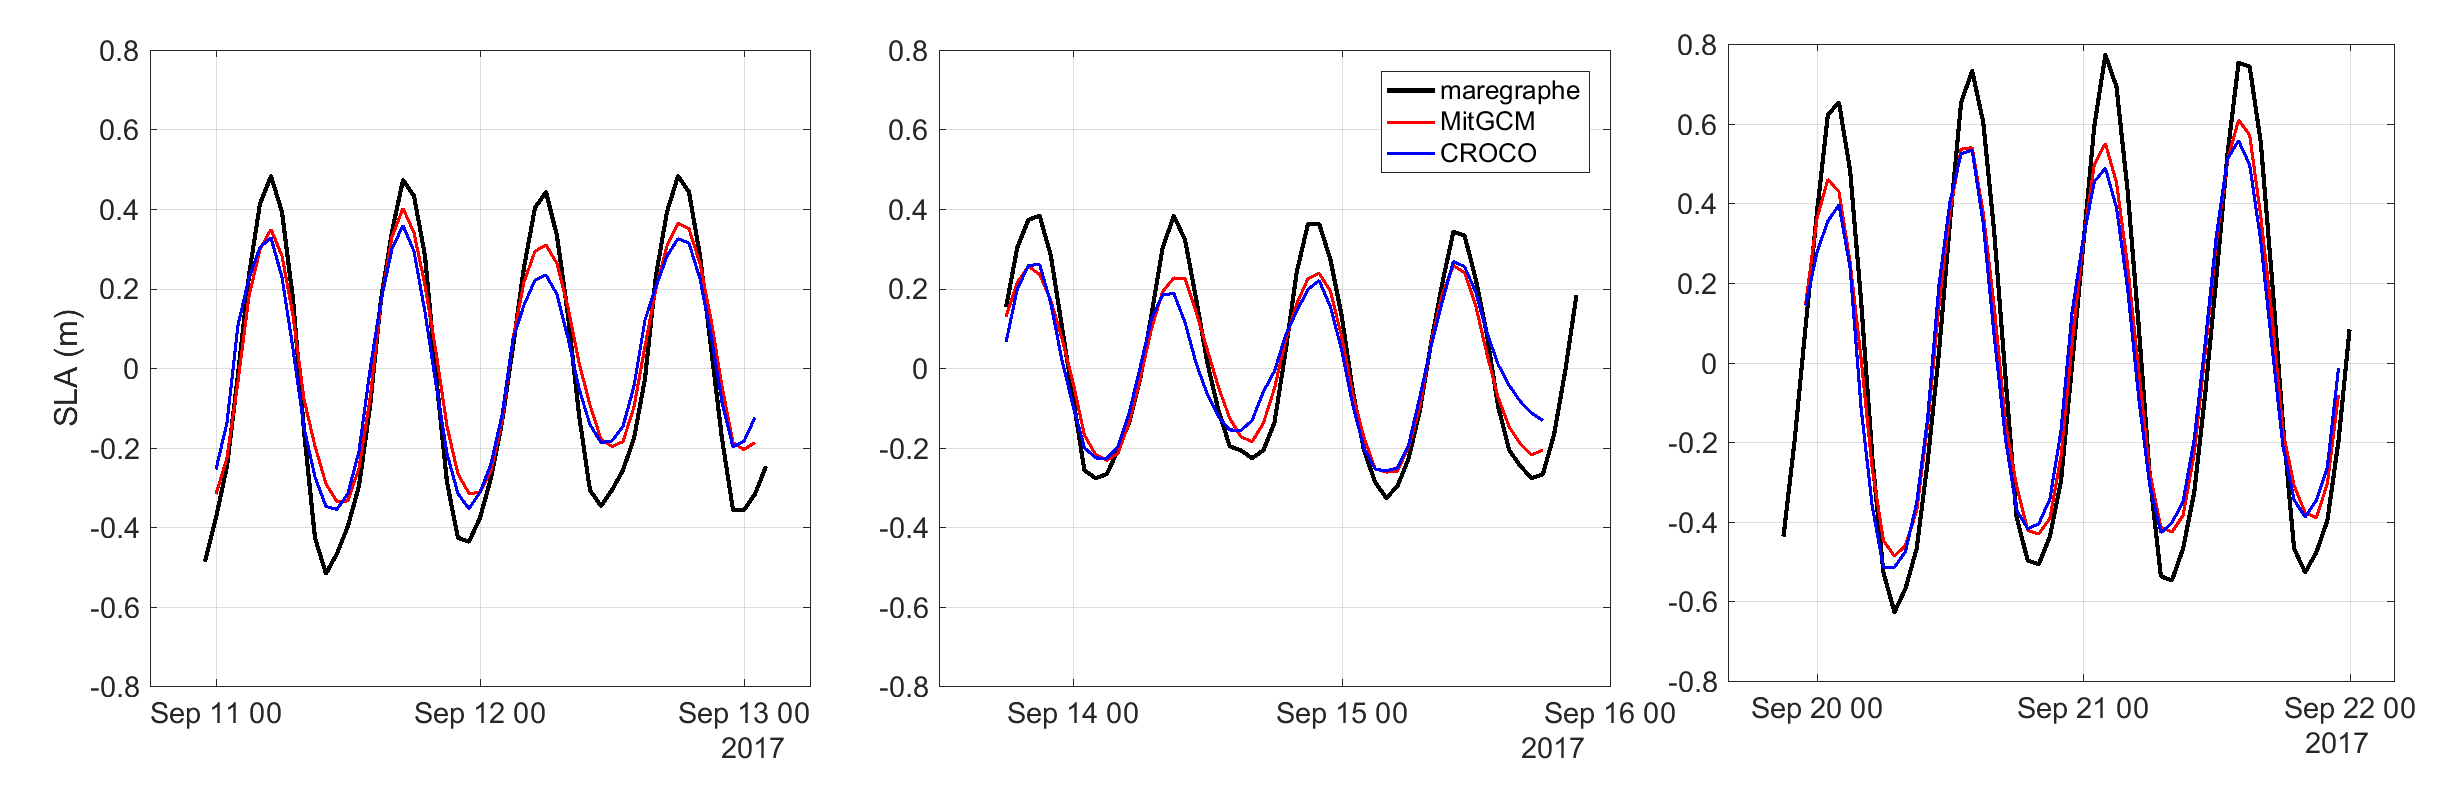
\includegraphics[width=\textwidth]{./GBR3D/SLA_Tarifa_ME2VE2IES.png}
        \caption{Sea level-anomaly at Tarifa from tidal gauge data (black) or at the nearest grid point for parent simulation (red) and CROCO simulation (blue), for situation ME (a), MM (b) et VE (c)}
        \label{fig_maree_tar}
\end{figure}

\subsubsection{Water masses}


\begin{figure}[!h]
        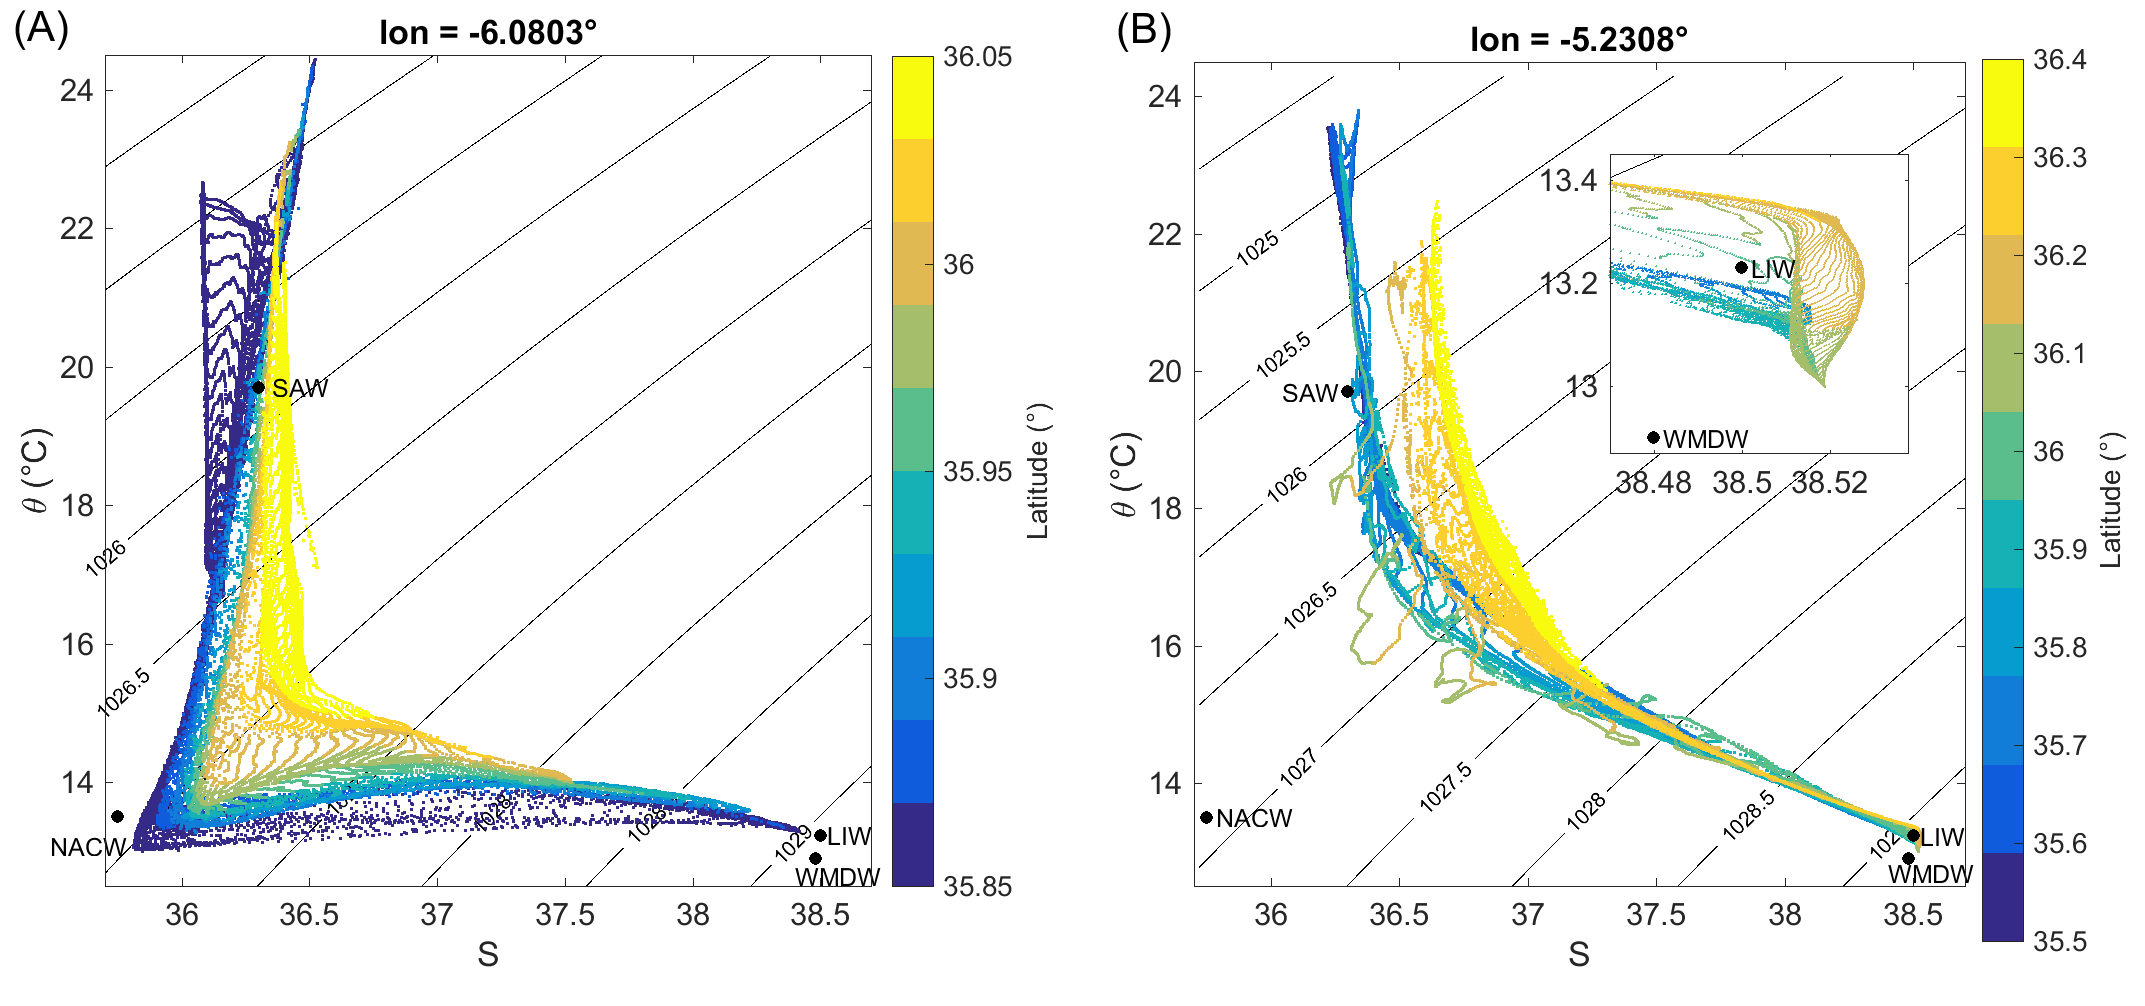
\includegraphics[width=\textwidth]{./GBR3D/WM_ini_IES.png}
        \caption{$\Theta$-S diagrams of grid points at 6.08$^\text{o}$W (a) and 5.23$^\text{o}$W in first timestep of SimIT, color indicates the latitude of each grid point. Are indicated cenroid definition of certain water masses according to Najanro2014}
        \label{Fig_Ini_WM3D}
\end{figure}


Figure \ref{Fig_Ini_WM3D} shows the $\theta$-S diagrams for east and west entry of the Strait in initial tracer field of simulation SimIT. As expected, for med waters see on the west side two signals for the two pathways of the med outflow, on the east side see distinctly a deep water mass and an intermediate one that could be interpreted as analogous to WMDW and LIW, with the latter being present mostly on the northern part, however in the simulation saltier and warmer waters than expected in bibliography. For atl waters, NACW present on west of domain, less on east. On east side, see difference surface water north/south of the opening of the Strait, with saltier surface waters in the north.




\subsection{Numerical diagnosis}
\label{PartDiag3D}

\subsubsection{Interface definition}

The analysis of simulation result is based on two layer definition of an Atlantic waters layer and Mediterranean waters layer. They are defined in regard to a reference salinity, with the interface defined as the height of the first water parcel from the top down in the water column for which salinity is above the reference salinity.

The reference salinity is taken as varying along the Strait as a hyperbolic tangent function of longitude centered at the Camarinal Sill to account for the different water mass composition in the eastern and western part of the Strait of Gibraltar. 

\begin{equation}
	S_i(x)=tanh(\frac{x-X_{CS}}{DX})\frac{S_M-S_m}{2}+\frac{S_M+S_m}{2}
\end{equation}
with $X_{CS}=5.75^o$, $dx=0.25^o$, the location and width of the Camarinal Sill in degrees, $S_M=37.39$ and $S_m=37.1$ the max and minimum values taken respectively east and west of the sill.

%This may not give the perfect interface at any given time...

\subsubsection{Froude layer number}

With the atlantic and mediterranean layers defined as above, the Froude layer number for internal gravity wave is computed at each 2D grid point as : 

\begin{equation}
F_i=\frac{U_i^2}{g'h_i} , \ \text{with} g'=g \frac{\rho_2-\rho_1}{\rho_0}
\end{equation}

where $\rho_i$ averaged density in layer i,  $U$ is averaged velocity norm over the layer i of height h. If $F_i>1$ say that the flow in layer i is supercritical.


\subsubsection{Hydraulic Jump detection, acceleration of flow}

\begin{figure}[!h]
 \centering
 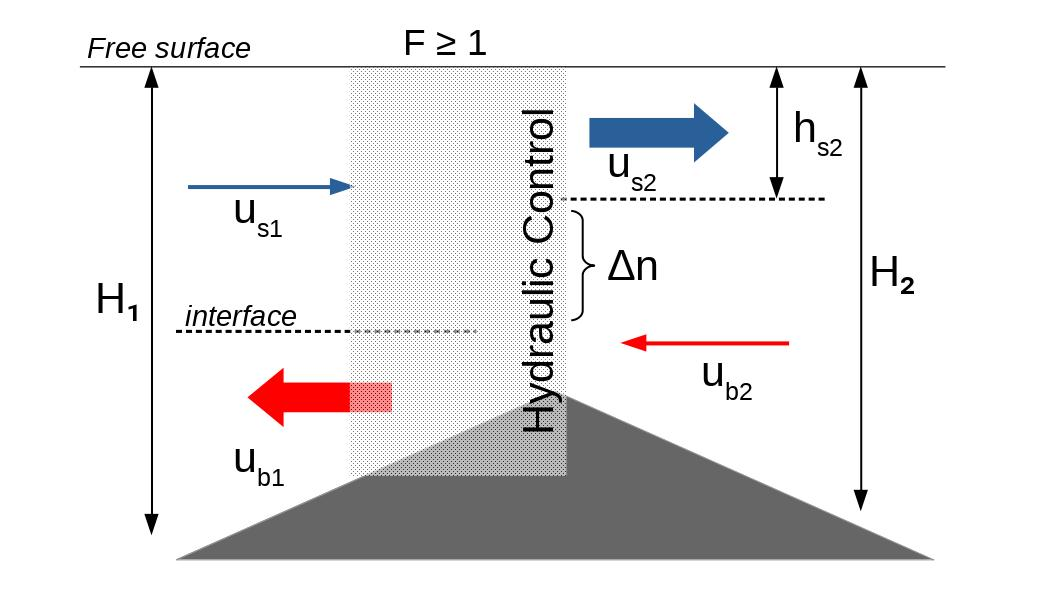
\includegraphics[width=0.5\textwidth]{./GBR3D/schema_diagressaut.jpg}
 \caption {Schematic of flow upstrean and downstream of hydraulic jump at Camarinal Sill, Strait of Gibraltar}
  \label{schemaRH}
\end{figure}


A simple diagnosis for detection of the hydraulic jump at Camarinal Sill in the simulations is based on the impact such a structure has on the flow. As shown/schematized/sketched(?) in figure \ref{schemaRH}, hydraulic jump (also called hydraulic drop) induces a drop of the interface depth. Since the flow in the Strait is canalised by bathymetry (for med flow) and coast (for atl flow), there must be conservation of flux from one section downflow and upflow of the hydraulic jump, which with the variation of the interface depth, means acceleration/deceleration of flow (depending on which layer is reference).

The drop in interface depth is noted $\Delta n=b_2-b_1$, the variation of bottom depth $\Delta H=H_2-H_1$ and the acceleration in the bottom layer $\Delta u_b = u_2-u_1$. For the bottom layer conservation of flux is :
\begin{subequations}
\begin{alignat}{2}
  \displaystyle
&u_1 (H_1-b_1)&& = u_2 (H_2-b_2)\\
& &&= u_1 (\Delta H + \Delta n) + u_1 (H_1-b_1) + \Delta u_b (H_2-b_2)
\end{alignat}
\end{subequations}

\begin{equation}
\Delta u_b = -u_1 \frac{\Delta H + \Delta n}{H_2-b_2}
\end{equation}

For the surface flow, similarly can find
\begin{equation}
\Delta u_s = - u_1\frac{\Delta n}{b_2}
\end{equation}

Velocity in the area of the hydraulic jump must validate condition of (at least) critical flow, ie Froude number $\geq$ 1. We search minimal condition for hydraulic jump so $F=1$, or $U=c$, taht is the flow ceerity equals the phase speed of internal wave. If for the latter we take the definition of interfacial speed can have an expression for $u_1$: 
\begin{equation}
|u_1|=c=\sqrt{g' \frac{(H_1-\Delta n - b_2)(\Delta n + b_2)}{H_1}}
\end{equation}



In the end, some parameters are chosen as threshold, here take values that should be correct for area of camarinal sill, the minimum excursion of the jump $\Delta n = 30m$ and the height of the Atl layer $b_2=50 m$ , and the reduced gravity $g'=0.02 m s^{-2}$.

\subsubsection{Q parameter and derivated diagnosis}

We want to detect primary shear instabilities in the Med outflow. A simple vorticity diagnosis is not chosen as it requires choosing the rotation axis, but also because regions of high shear such as between the MEd outflow and Atl waters will have high vorticity values. Instead, analogously to the use of the Okubo-Weiss parameter in Hilt 2020, we chose to compute parameter Q, defined as (ref):

\begin{equation}
Q=-\frac{1}{2} \frac{\partial u_i}{\partial x_j} \frac{\partial u_j}{\partial x_i} = \frac{1}{2} (\Omega_{ij}\Omega_{ij} - S_{ij} S_{ij})
\end{equation}
with $u_i$ the components of velocity vector, and $S_{ij}$ and $\Omega_{ij}$ are respectively the strain-rate tensor and vorticity tensor. When $Q>0$, rotation is predominant over shear part.


Due to advection by the Med outflow, a succession of primary instabilities will propagate over teh same grid cells. The temporal evolution of Q over such grid cell will show oscillations between high positive value (center of a billow/vortex) and low negative values (shear between two consecutive billows). A proxy to detect this area is chosen as high value of standard deviation of parameter Q, as defined in equation \ref{eqstdQ} where the over bar denotes temporal average over 30 minutes, a period over which there will be minimal modification of the general flow in the Strait.

\begin{equation} 
\label{eqstdQ} 
    std ( Q ) (\vec{x},t)=  \sqrt{   \overline{Q (\vec{x},t)^{2}} -  \overline{Q(\vec{x},t)}^{2}  }
\end{equation}

To create 2D maps presented in next section, only the maximal value of standard deviation in the water column is saved...
By implementing this calculation directly in the code, we can asses where instabilities/vortexes propagate without having to make a huge volume of simulation outputs over the whole domain, those economising in storage place and data readability. 

The result of this proxy can be compared to the result of the Singular Value Decomposition (SVD) of the time-varying 3D field. However this calculation is off-line and necessitates a high frequency 3D output to pick up the relevant structures.



\subsection{Results}
\label{section3DRes}

\subsubsection{Flow criticality/Hydraulically controlled layer and hydraulic jump, neap-spring tide variability}


\begin{figure}[!h]
 \centering
 
 \begin{subfigure}{\linewidth}
\centering
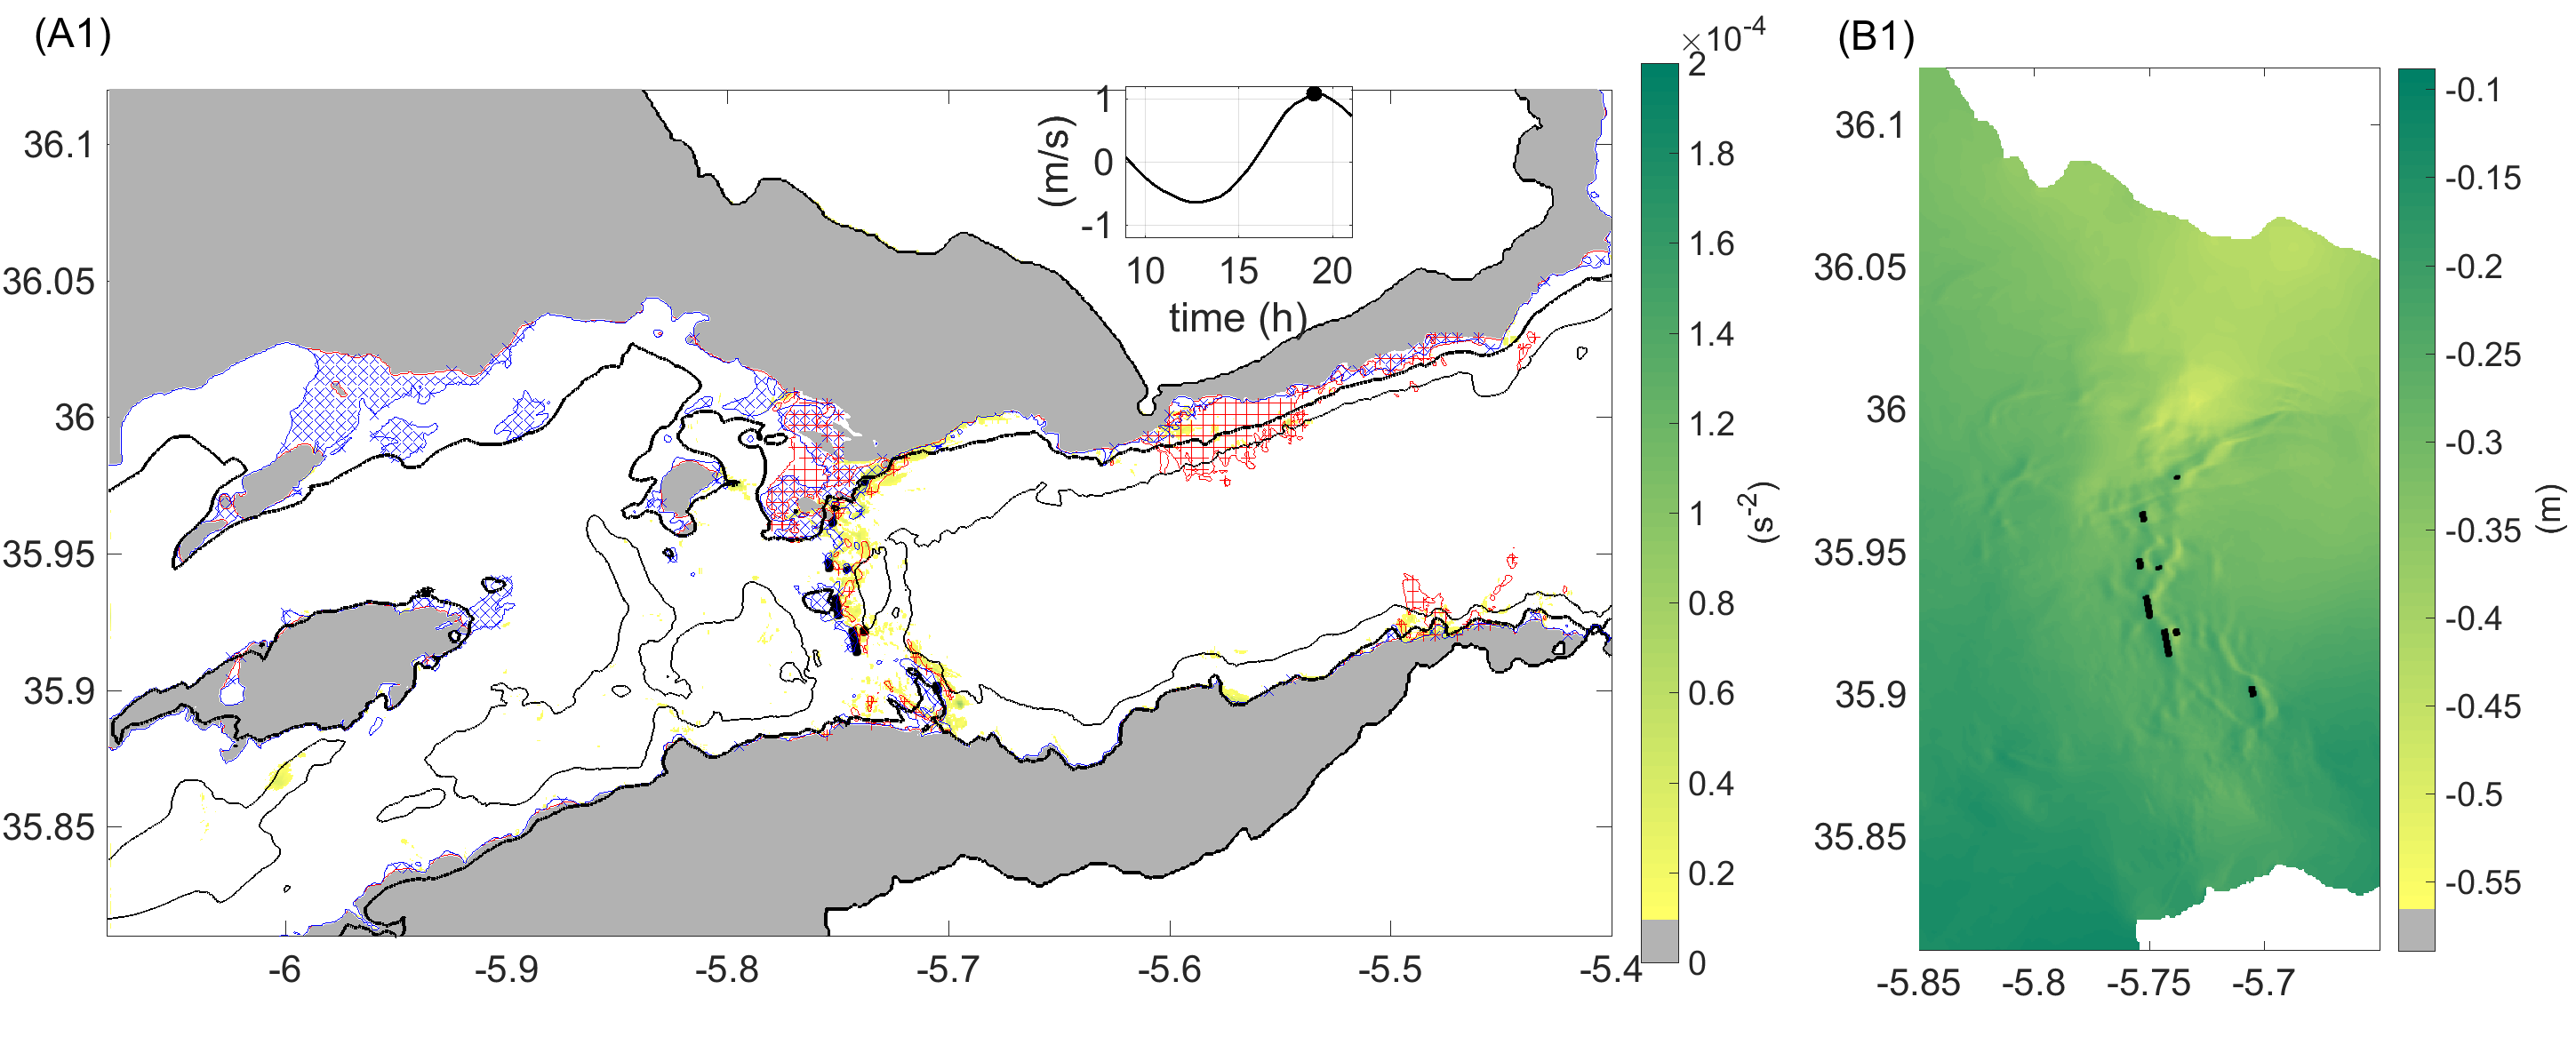
\includegraphics[width=1\linewidth]{./GBR3D/ME2_19h_p.png}
\end{subfigure}
 
 \begin{subfigure}{\linewidth}
\centering
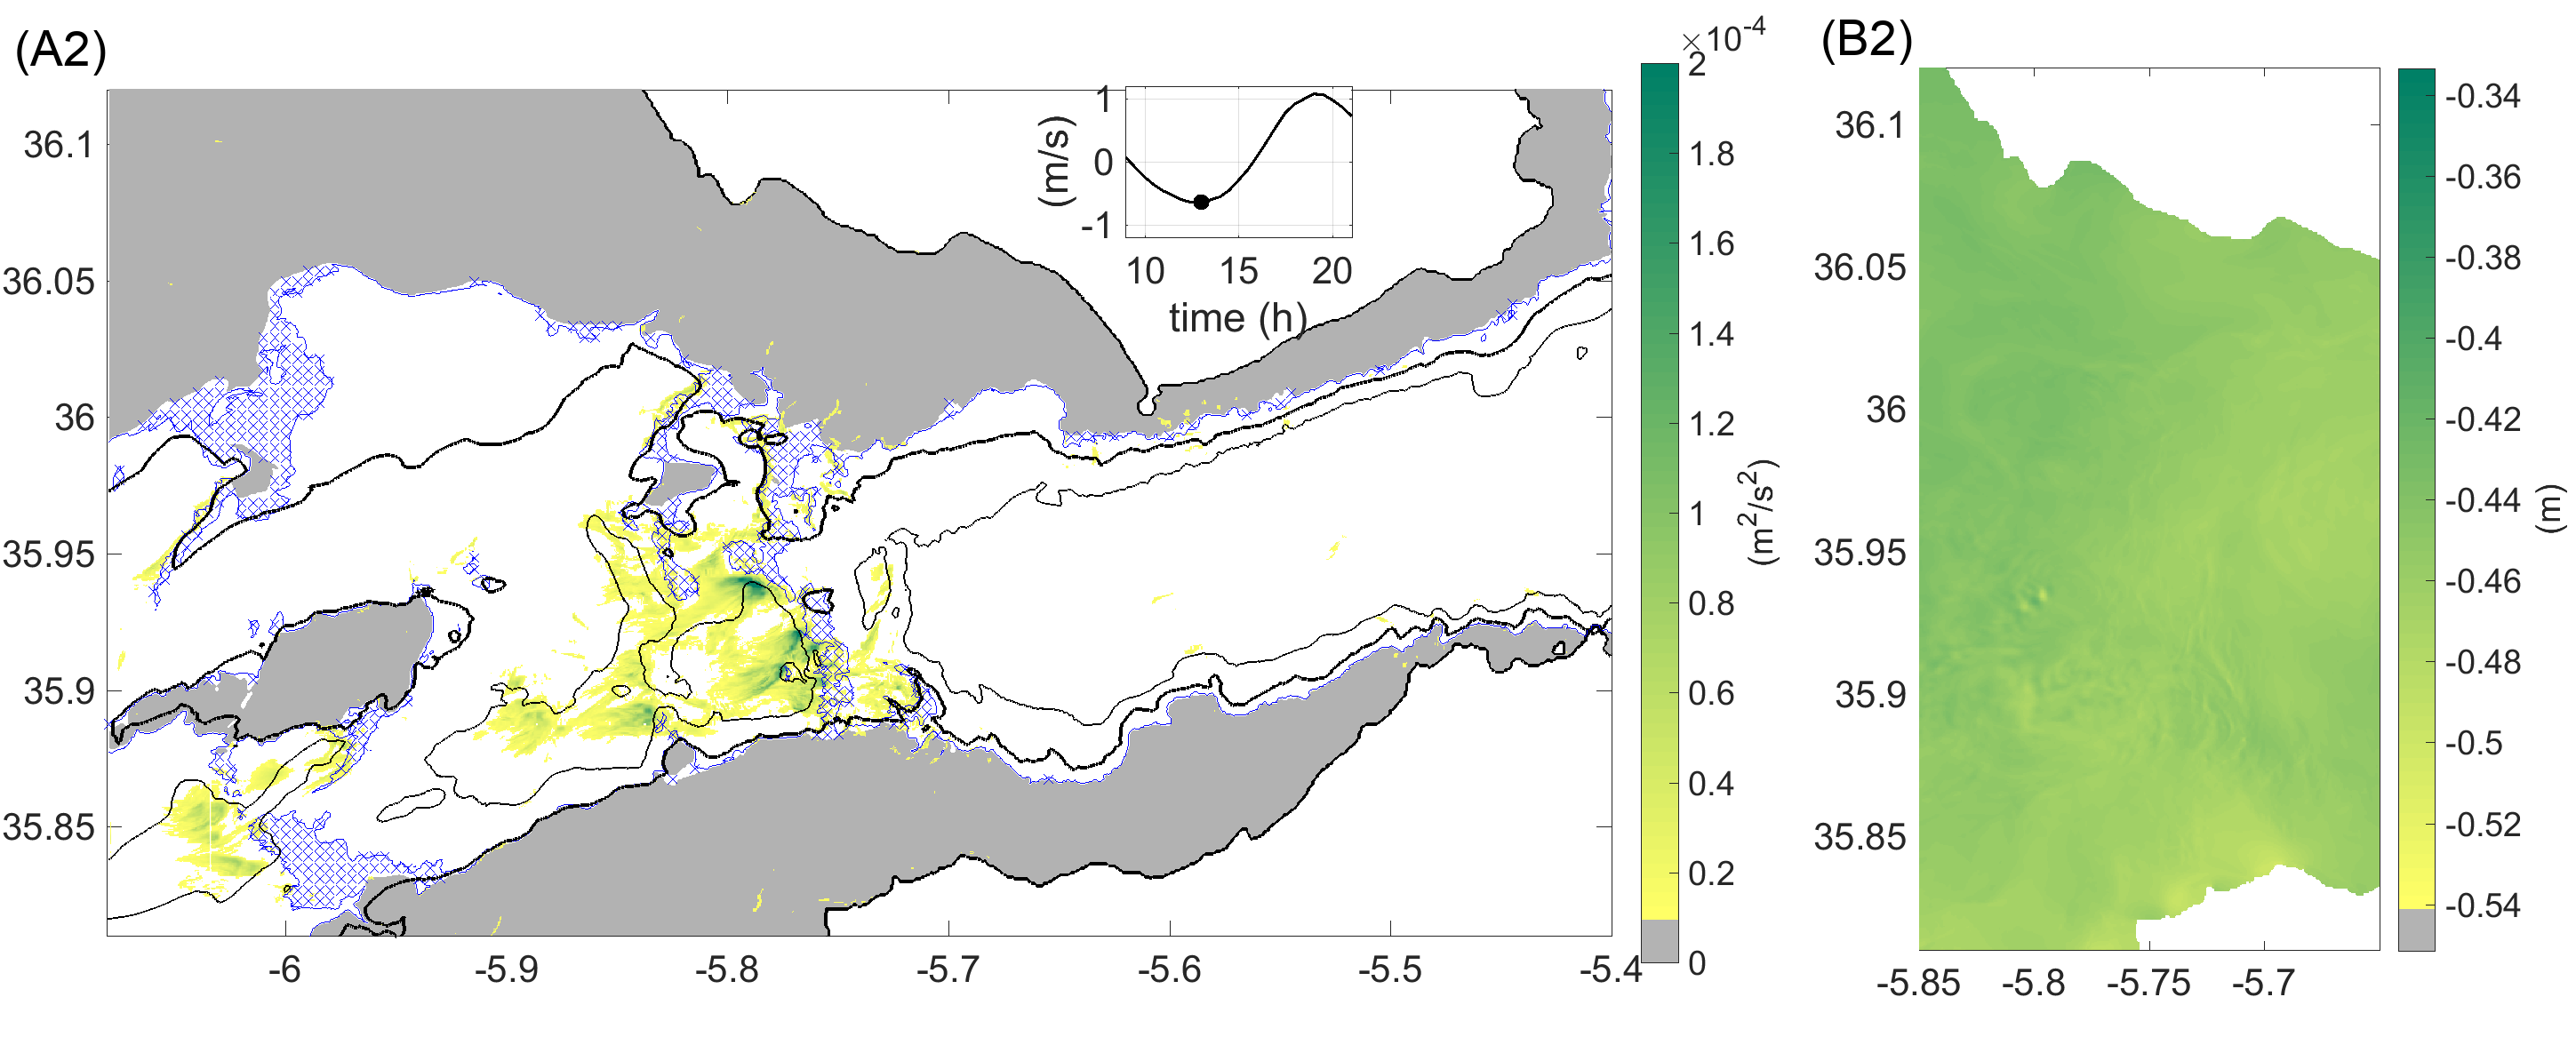
\includegraphics[width=\linewidth]{./GBR3D/ME2_13h_p.png}
\end{subfigure}
\caption {For simulation SimNT, an inflow then an outflow of type \textit{no-jump}. Blue (red) shaded area is supercritical med (atl) layer. Black dots are hyd jump detection. grey area denotes where S bottom$<$Sinterface. colorbar for standard deviation of parameter Q (only values above $10^-5$are represented). Also inicated barotropic znal current at CS (point indicated in figure \ref{FigBathy3D}). Two black isobathes contours are indicated, 200m (bold) and 400m(thin) depth  }
\label{FigHCN}
\end{figure}

Figures \ref{FigHCN} to \ref{FigHCI} present several diagnosis for series of maximal outflows and inflows for variable strength of the tidal forcing among simulations SimNT,SimST then SimIT. Are represented the diagnosis presented in paragraph \ref{PartDiag3D} : the area of supercritical flow in atl and med layer as shaded areas, the detection of hydraulic jump, and area of standard deviation of parameter Q, which indicate were vortices are propagating. The grey area indicates where the salinity in the bottom level is below the interfacial salinity as defined in paragraph ..., and thus were it is considered only Atlantic waters circulate.

Figure \ref{FigHCN} presents a situation of weak barotropic currents ($<1m/s$ at a shallow point of Camarinal Sill) in outflow and inflow and is considered a 'neap-tide' case, figure \ref{FigHCS} is for strong barotropic currents ($\geq 1.5m/s$) for the in- and outflow of a 'spring-tide' case. Finally, figure \ref{FigHCI} is the case of an outflow for an intermediate strength ($\approx 1m/s$)of the barotropic currents.

\begin{figure}[!h]
 \centering
\begin{subfigure}{\linewidth}
\centering
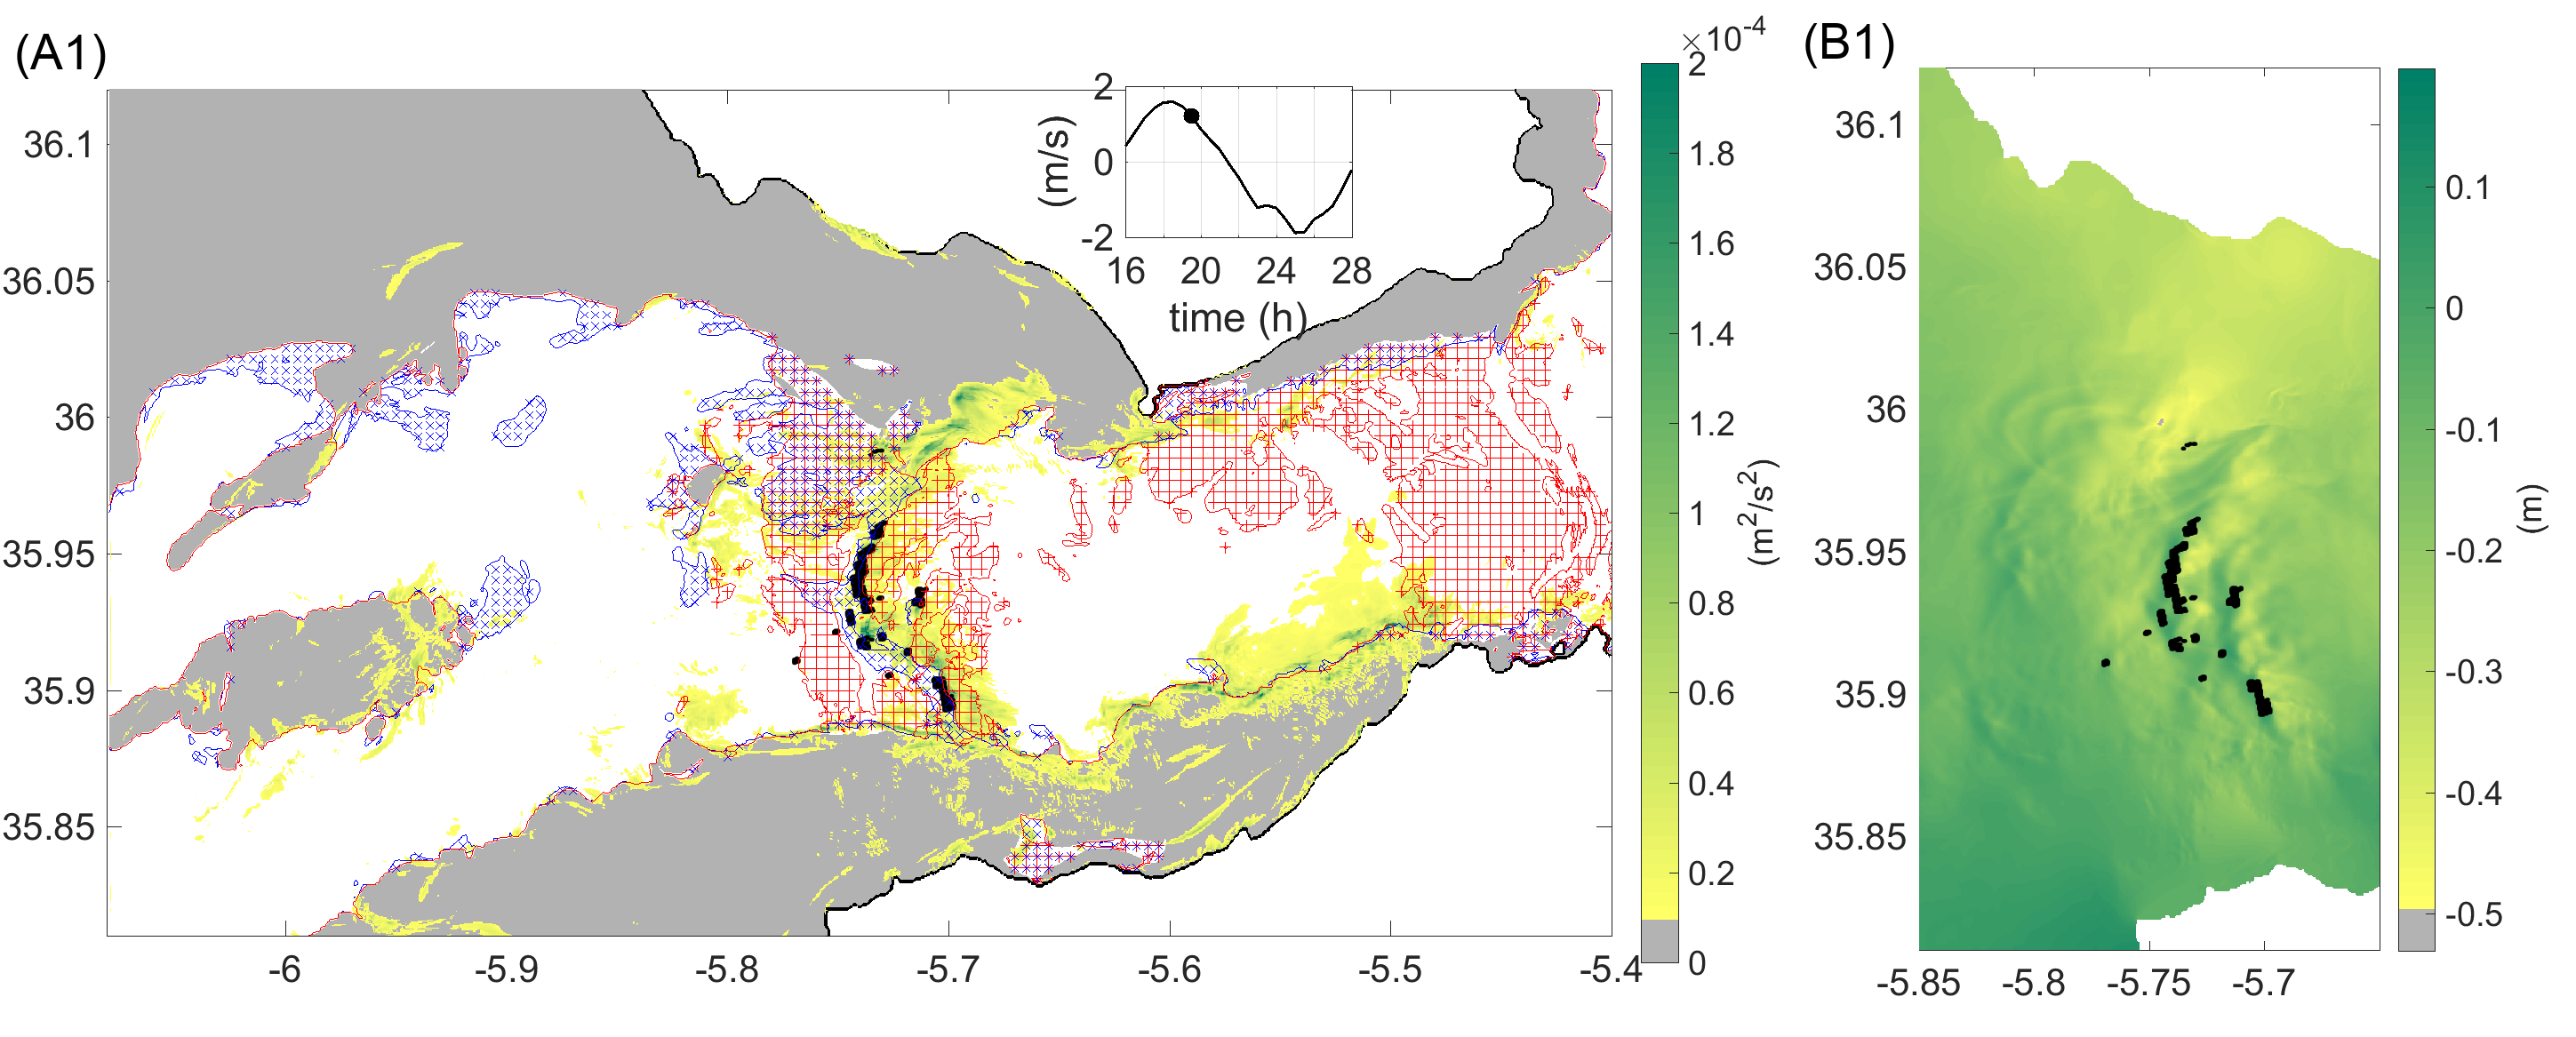
\includegraphics[width=\linewidth]{./GBR3D/VE2_19h30_p.png}
\end{subfigure}

\begin{subfigure}{\linewidth}
\centering
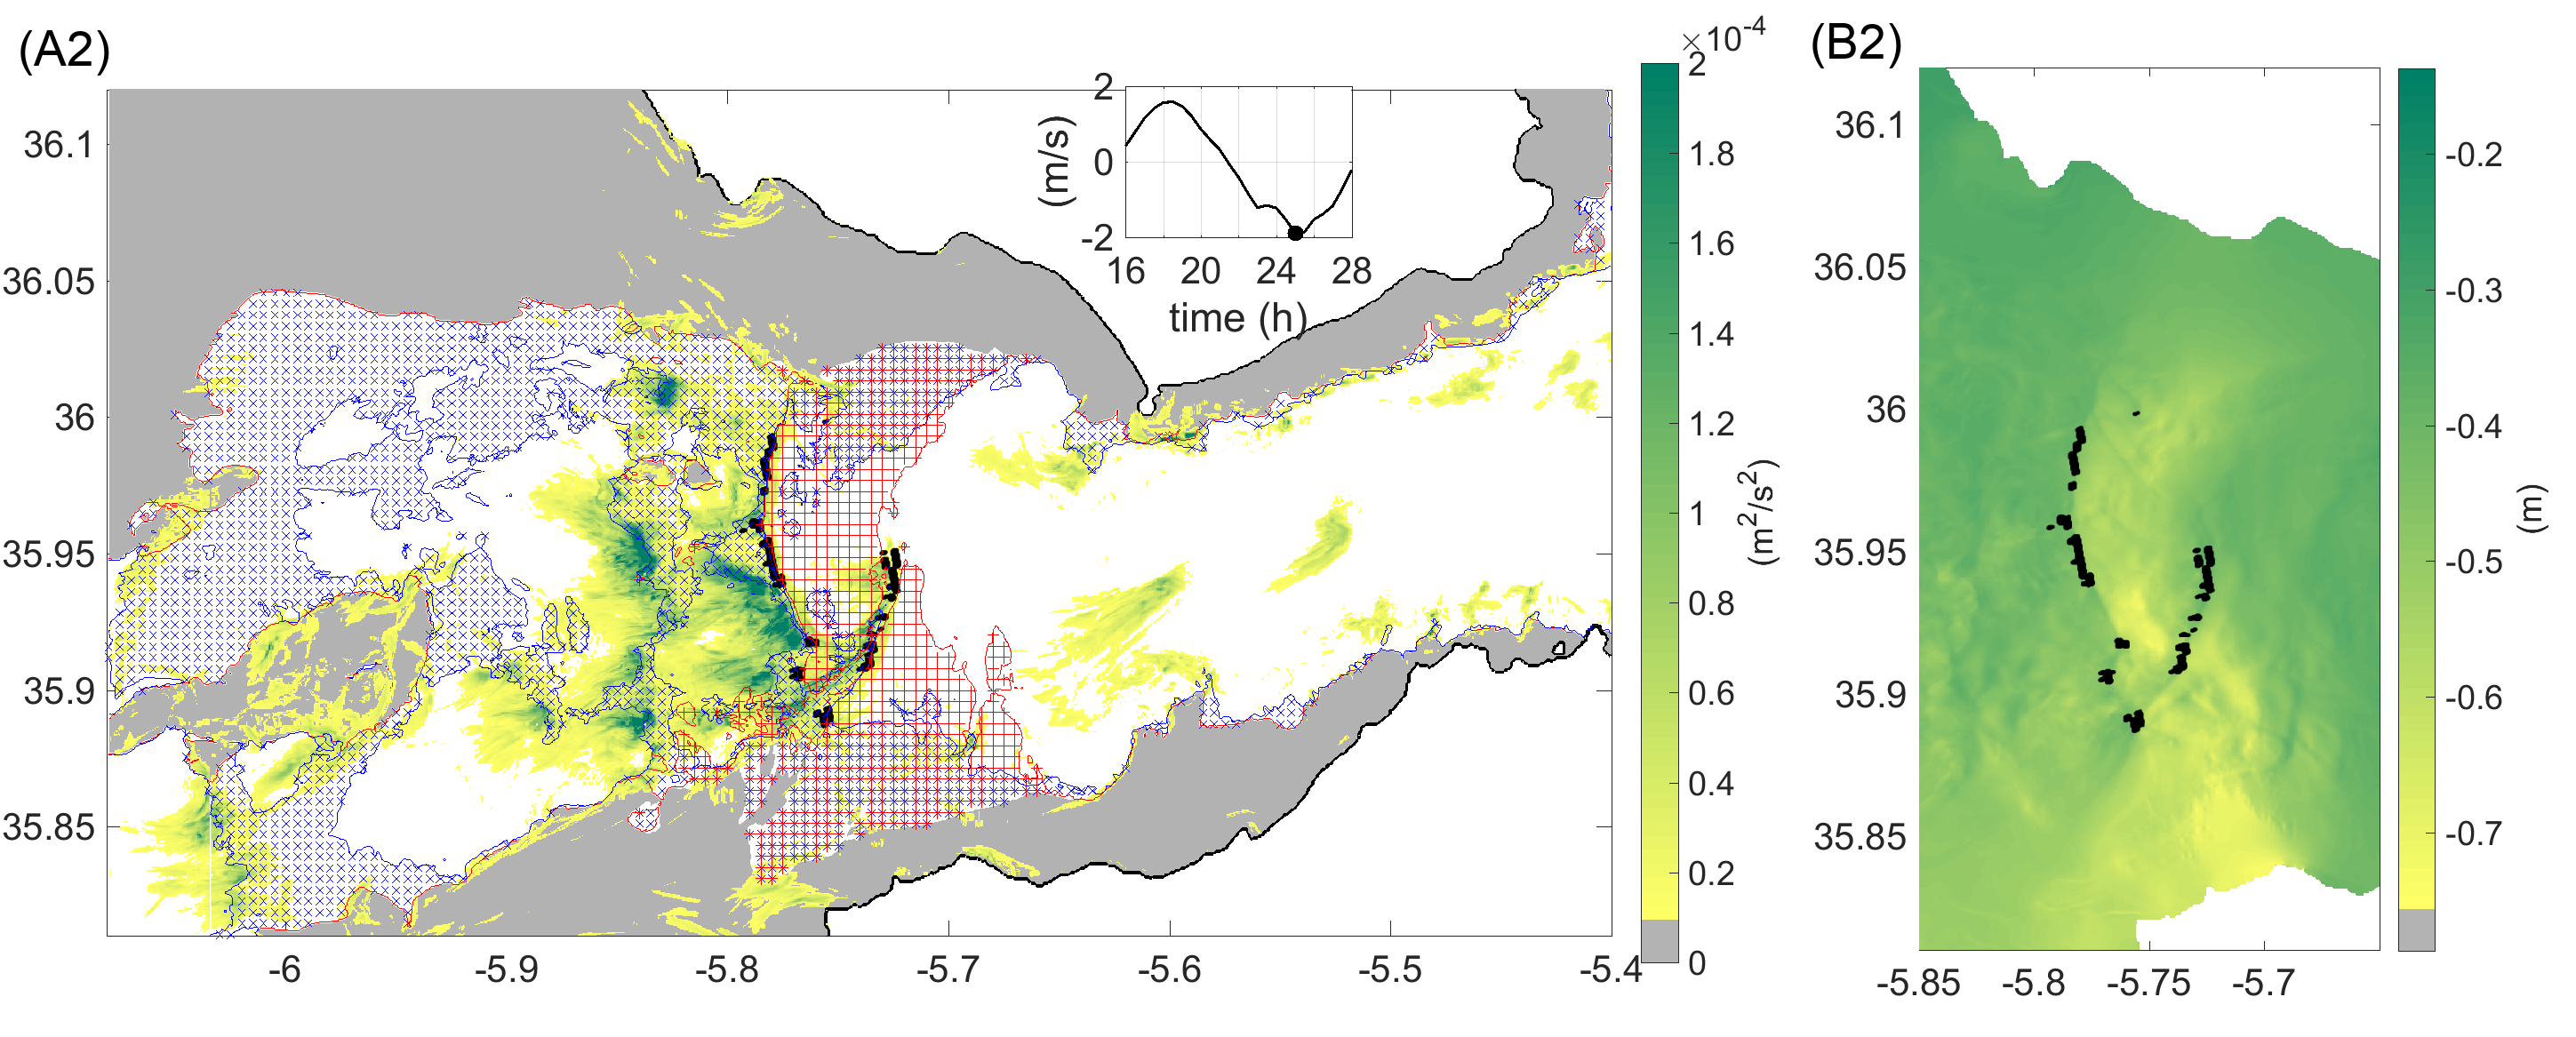
\includegraphics[width=\linewidth]{./GBR3D/VE2_25h_p.png}
\end{subfigure}
\caption {Same as figure \ref{FigHCN} for simulation SimST in inflow and outflow of type \textit{w-jump}}
\label{FigHCS}
\end{figure}

\begin{figure}[!h]
 \centering
%\begin{subfigure}{\linewidth}
%\centering
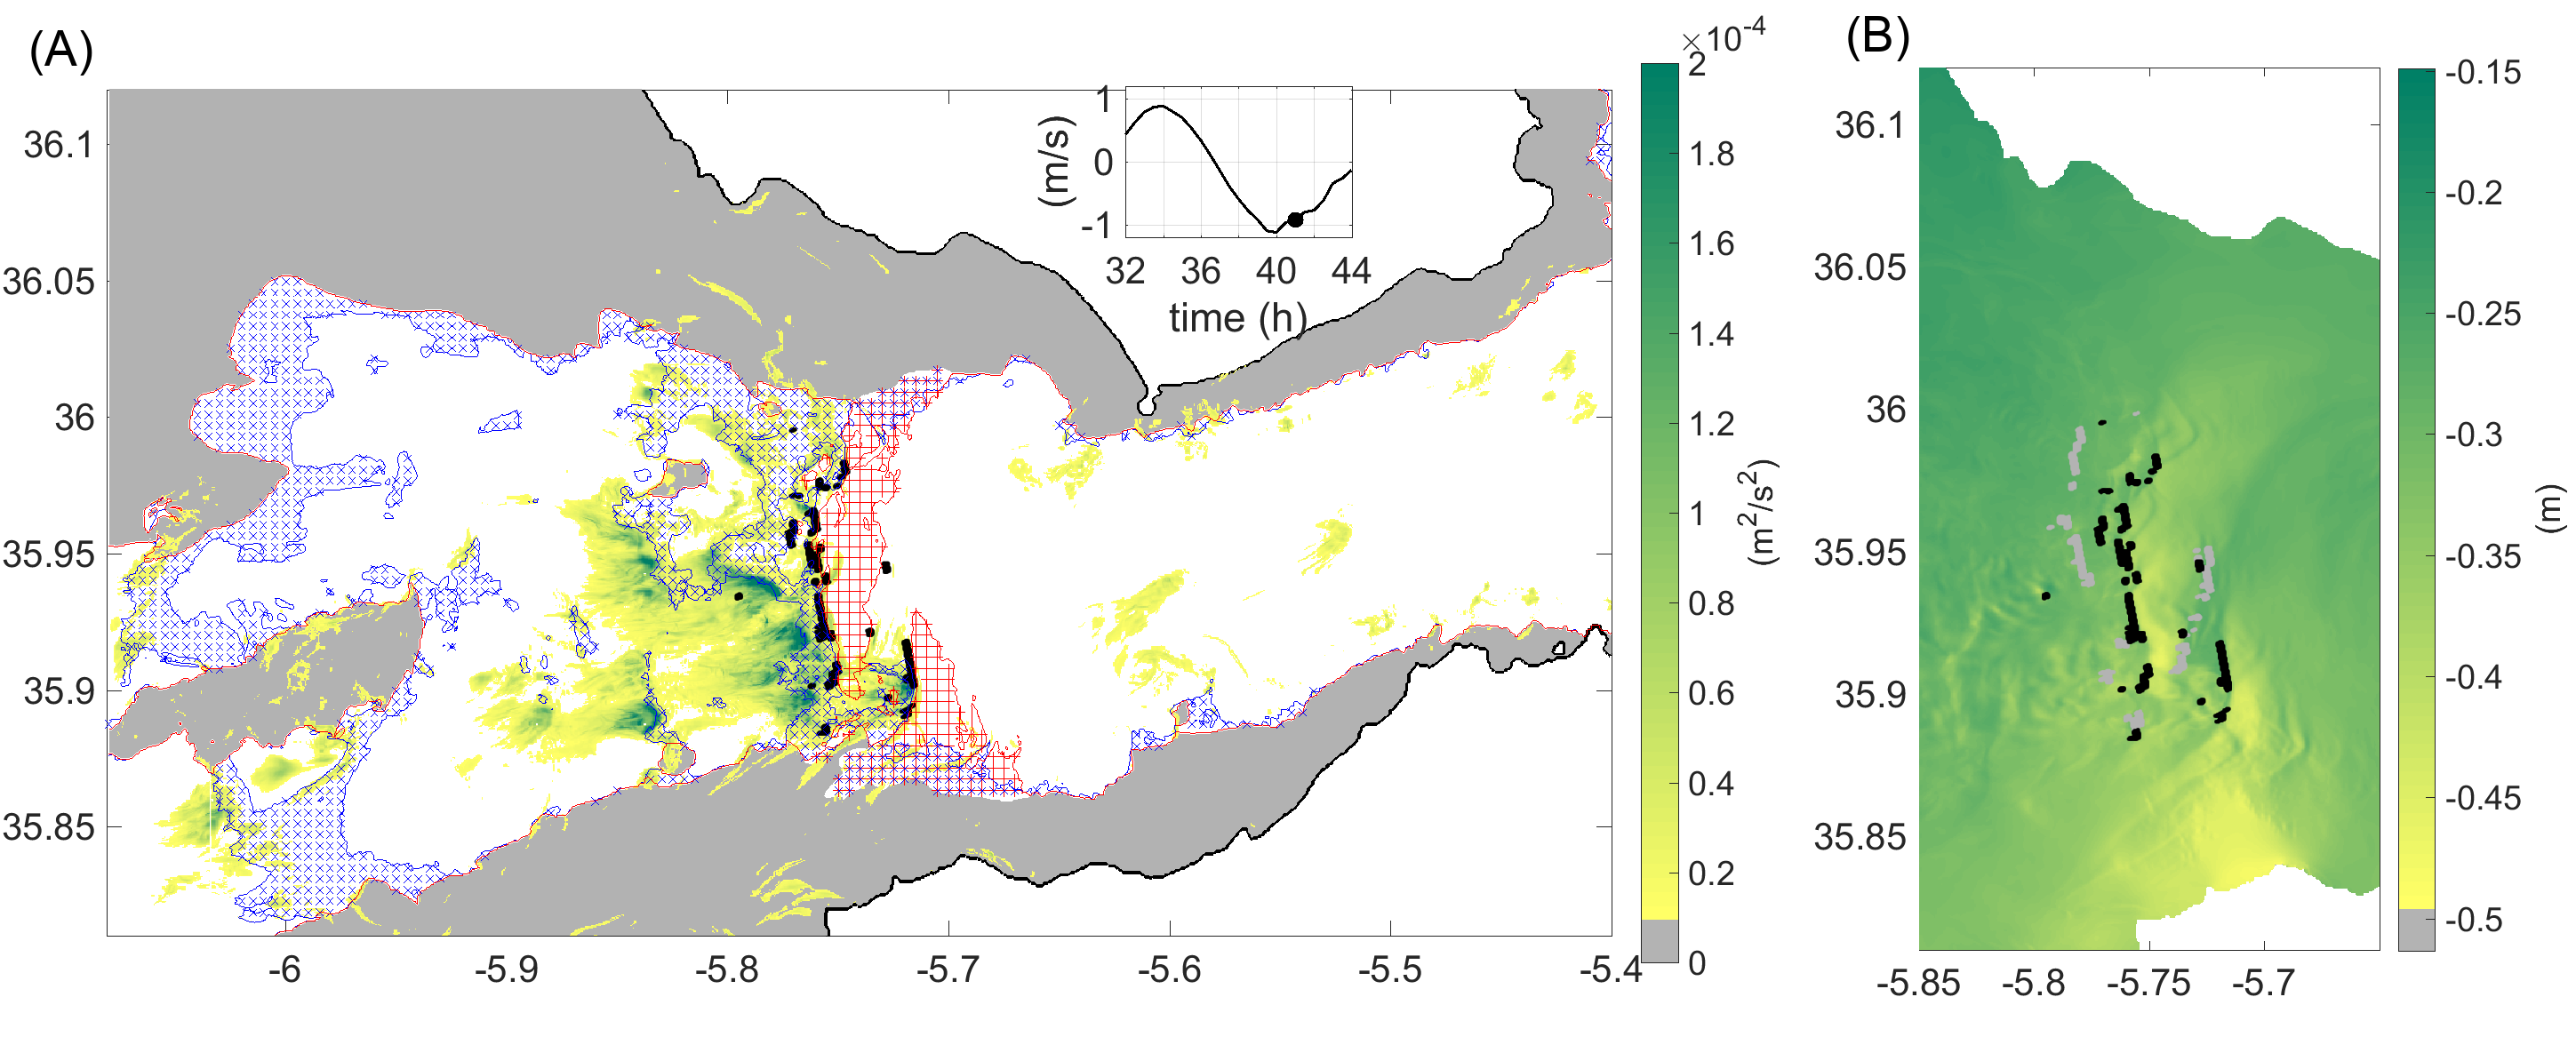
\includegraphics[width=\linewidth]{./GBR3D/IES_41h_p.png}
%\end{subfigure}
 \caption {Same as figure  \ref{FigHCN} for simulation SimIT and an outflow of type {s-jump}, on figure SLA also put trace of jump of spring tide outflow}
 \label{FigHCI}
\end{figure}

Firstly, can see two channels west of the Camarinal Sill where Med layer is present, separated by Majuan Bank. The path of the med vein through the south channel does not change much, however in the northern channel see a variable area of circulation for med waters above 200m depth and centered at 36$^\text{o}$ N. This area is larger during outflows, as med waters are driven up-slope by the westward barotropic current, but there is also a southern component to the flow that bends back into the main north channel (see figure \ref{FigBathy3D} for a better view of the bathymetry of the area).

For all cases, supercriticality of the atlantic (mediterranean) layer happens mostly east (west) of 5.8$^\text{o}$W which is the western slope of Camarinal sill. During inflows in figure \ref{FigHCN}.a and \ref{FigHCS}.a, criticality of the mediterranean layer only occurs in patches, the most extended one in the area of the northern channel discussed above. In outflows in figures \ref{FigHCN}.b,\ref{FigHCS}.b and \ref{FigHCI} the Mediterranean layer is supercritical at both Camarinal, Espartel Sill and northern channel for all cases. In the spring tide outflow case especially, most of the northern channel has a supercritical flow while at Espartel there is not much difference between the intermediate and spring tide outflow cases.


During outflow supercritical atl layer only at CS, except in neap case where it does not occur at all. In the case where both layers are supercritical at CS, hydraulic jump is detected. It is located at the junction between an area where atl and med layer are supercritical. It follows area of high gradient of free surface elevation.  Find accross all simulated tidal cycle three type of flow at Camarinal Sill during outflow : no hydraulic jump as in figure \ref{FigHCN}.b (\textit{no-jump}), a hydraulic jump situated just above the sill (figure \ref{FigHCI}, \textit{s-jump}), and a hydraulic jump situated over the west slope of the Camarinal Sill (figure \ref{FigHCS}.b, \textit{w-jump}). In this latter case, the hydraulic jump actually starts forming over the sill's crest as in the s-jump case but as the tidal currents strengthen, the area of supercritical atl layer area develops westward and so does the junction where can observe the jump.

Also see hydraulic jump during inflows, located in the same area over the east slope of CS regardless of the strength of tidal currents, but more pronounced with stronger barotropic currents, associated with transition of flow upstream of area of supercritical atl layer.

East of Camarinal Sill, another area of supercritical Atl layer appears during inflows. In neap-tide case, as a patch near north shore in TN at 5.59$^o$W. for spring tide case, this patch is more extended, and a secondary area of supercritical atl flow exists between 5.5$^o$W and 5.4$^o$W, extending from the north to the south side of TN. 

Figure \ref{FigISWGBR3D} shows the field of surface current divergence in Tarifa Narrows while a train of ISW is propagating, figure a for condition of intermediate strength of barotropic current in inflow and figure b for a strong barotropic current at the same time as figure \ref{FigHCS}.b. Are also shown the areas of critical atlantic layer flow as black meshed area. The propagation of the ISW train occurs at the same time as maximum inflow in this area and see the area of atl layer criticality is west of the propagating wave train . It seems the northern part of the criticality of the atl layer is dissociated from its southern part. The former occurs most often and is more or less extended while the other may be affected by influence of the passage of the ISW, either due to induced velocity or change of stratification.



\begin{figure}[!h]
 \centering
%\begin{subfigure}{\linewidth}
%\centering
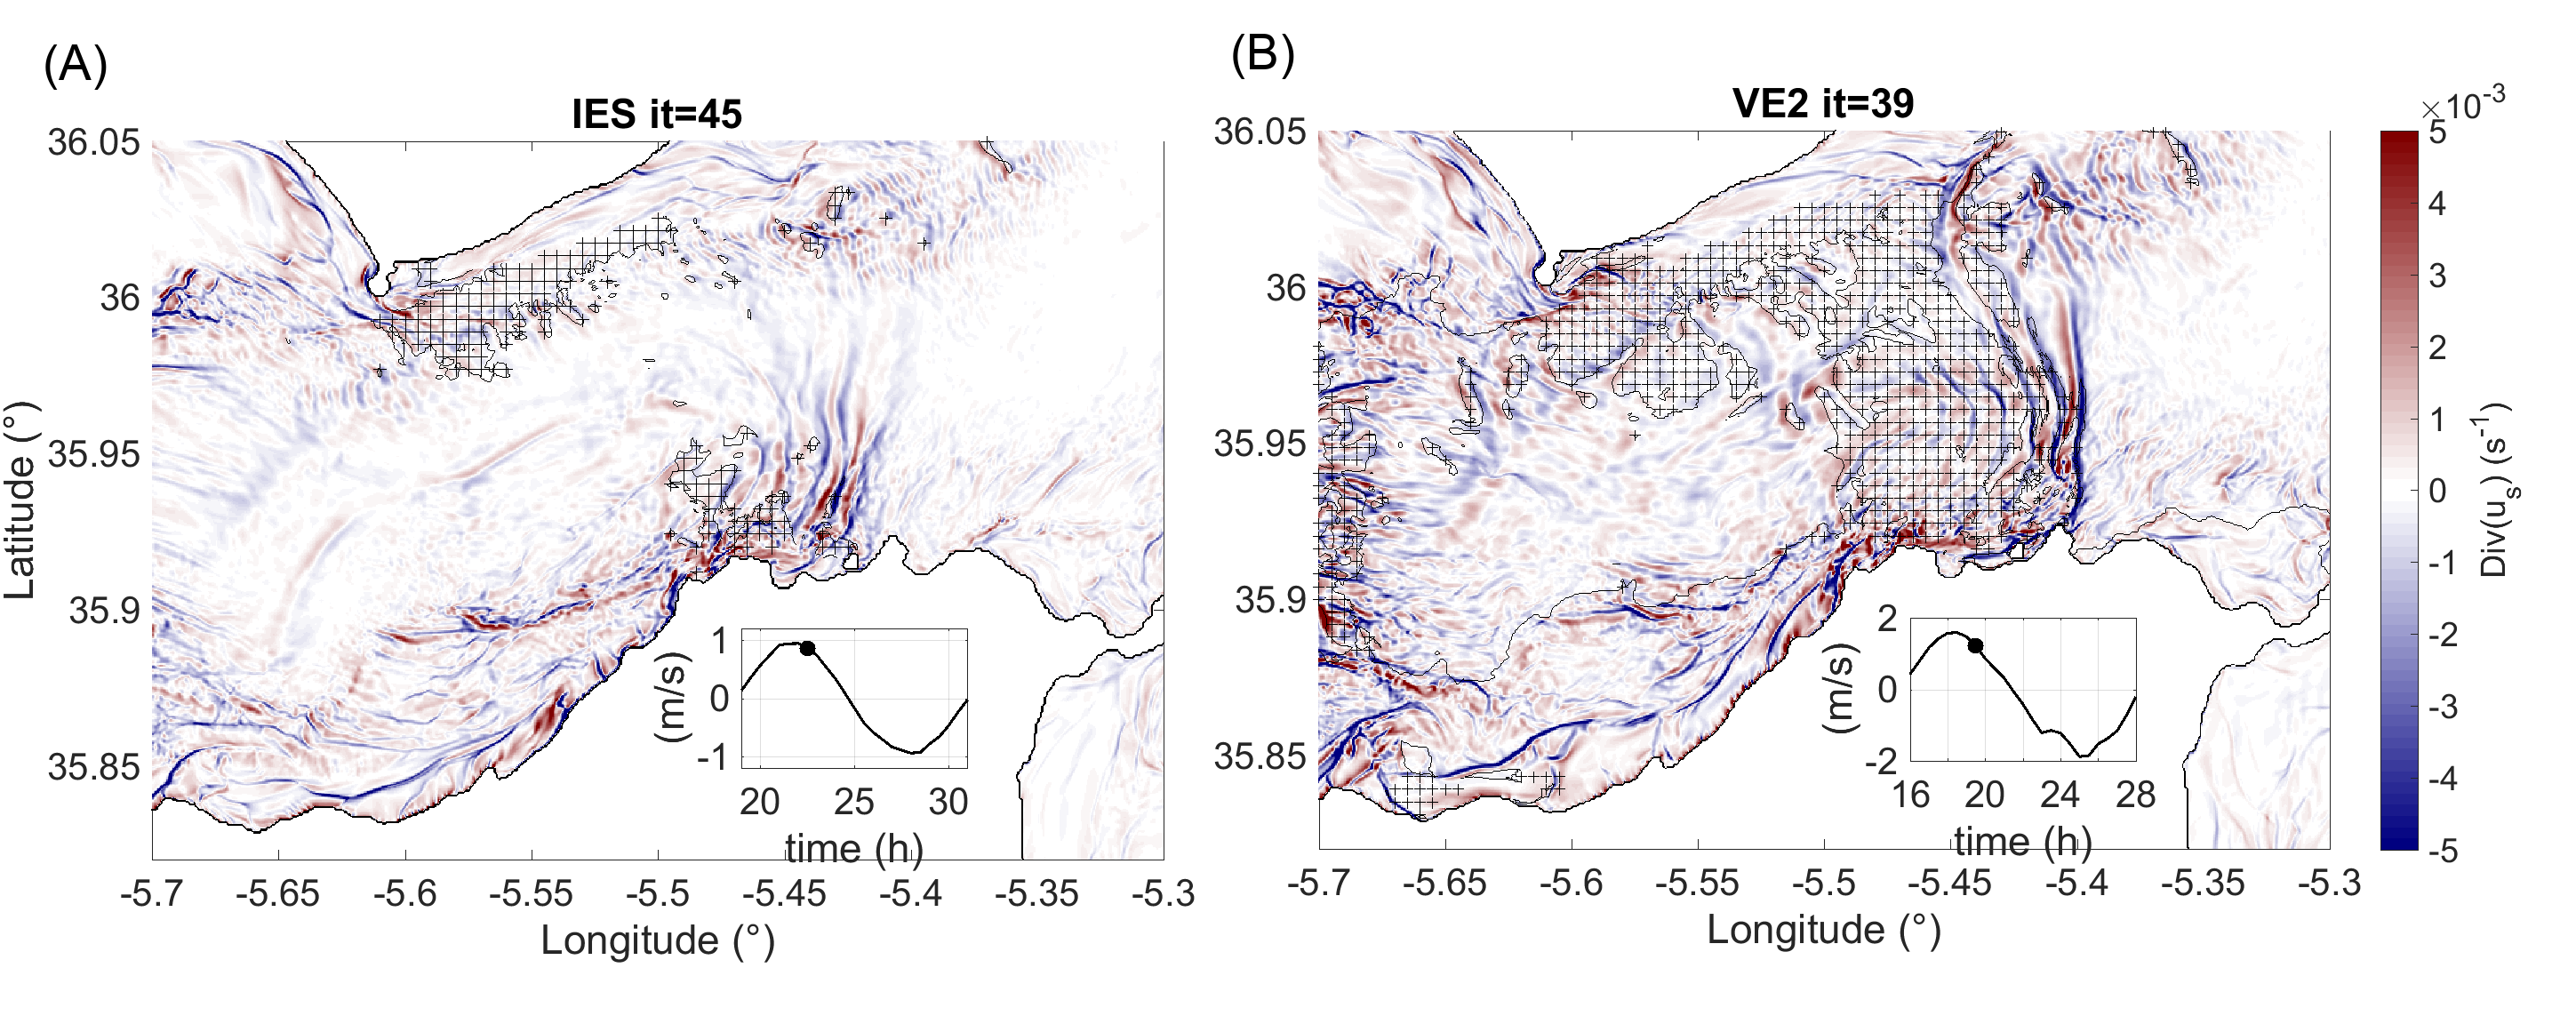
\includegraphics[width=\linewidth]{./GBR3D/FigWaveCont.png}
%\end{subfigure}
 \caption {Divergence of surface current (color) and area of supercritical atlantic layer (black hatchs) at t=22.5H in SimIT (a) and t=19.5H in SimST (b)}
 \label{FigISWGBR3D}
\end{figure}


\subsubsection{Propagation of Solitons (ISWs)}



\begin{figure}[!h]
 \centering
 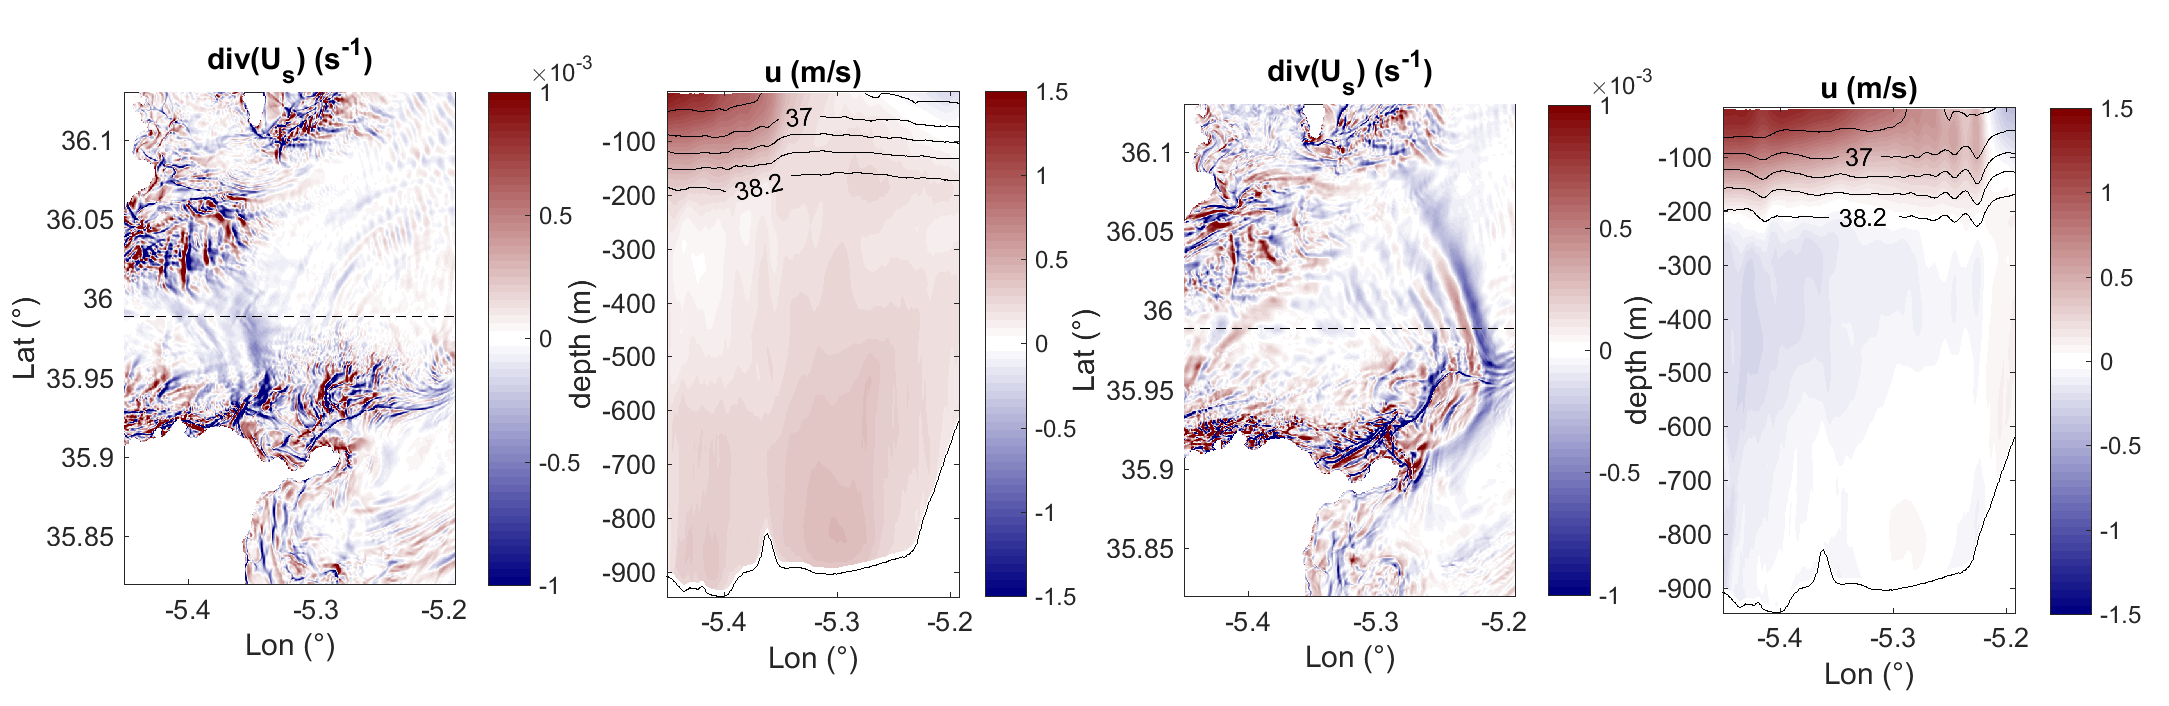
\includegraphics[width=1.\textwidth]{./GBR3D/coupesISW_ME2-2.png}
 \caption {Divergence of surface current (a,c) and vertical section (b,d) of salinity (black ishalines) and zonal velocity $u$ (color) in SimNT at 20h (a,b) and 22h (c,d) of simulation.}
  \label{FigISWNT}
\end{figure}



\begin{figure}[!h]
 \centering
%\begin{subfigure}{\linewidth}
%\centering
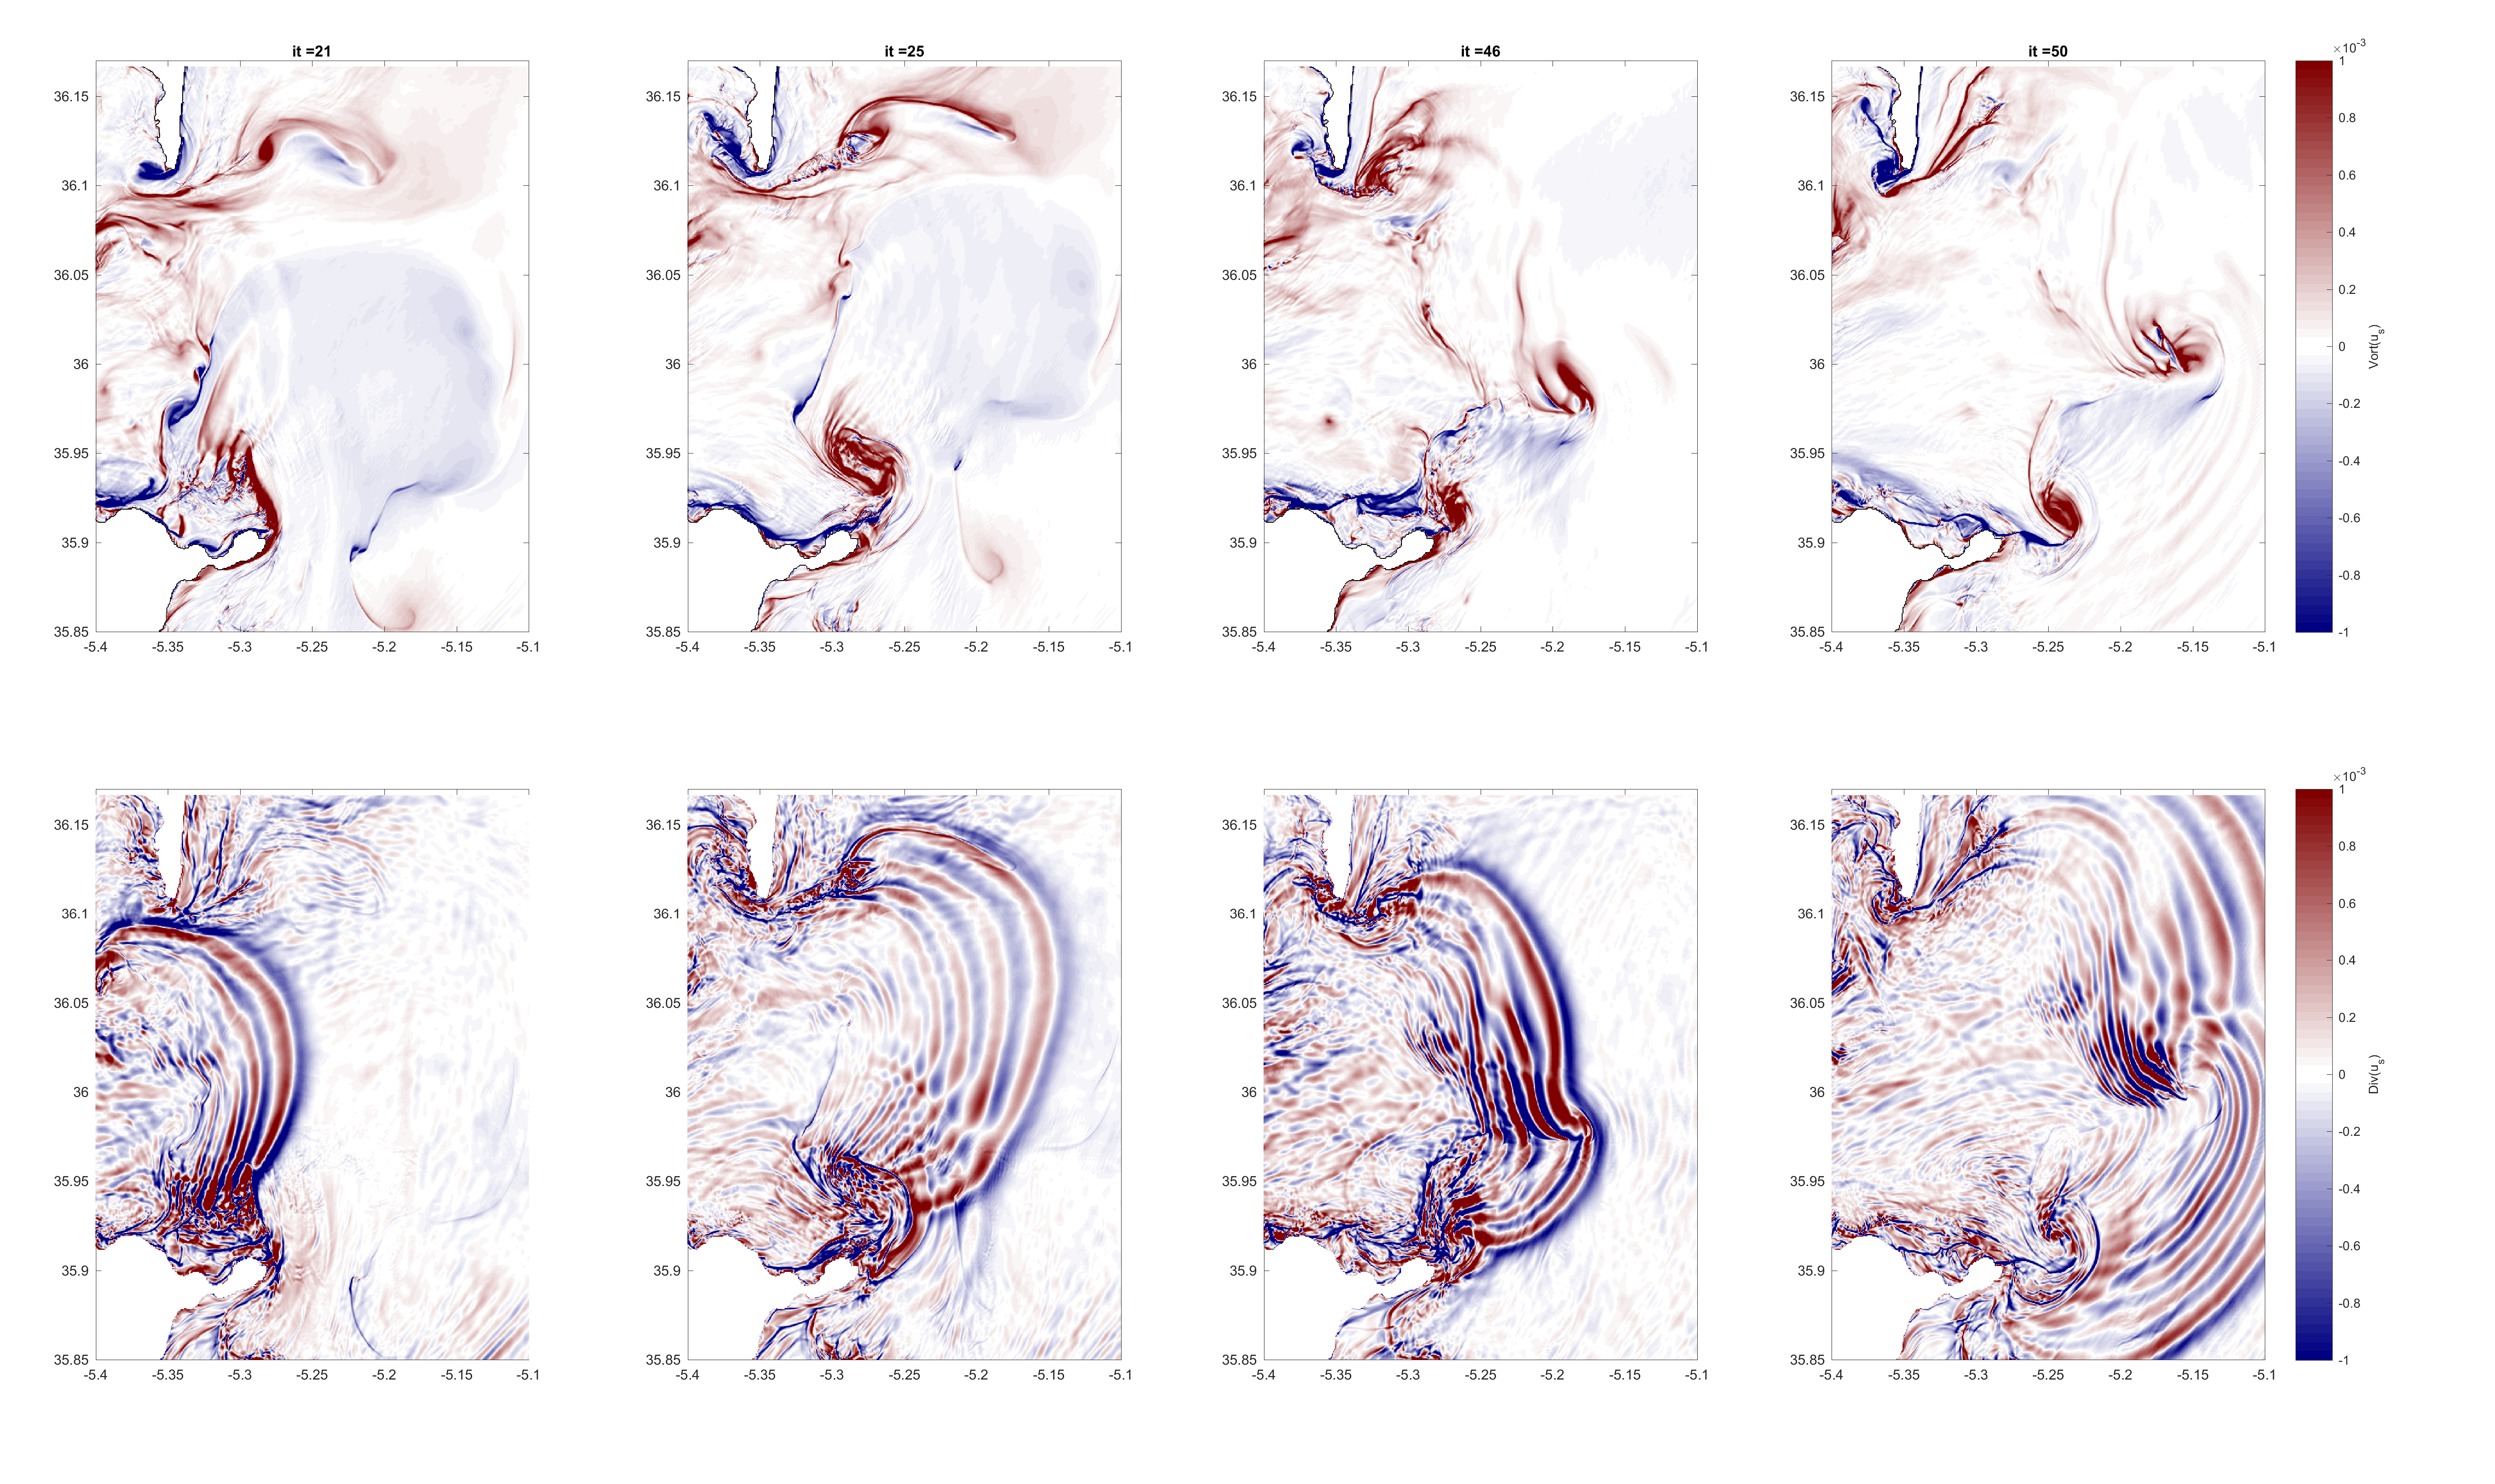
\includegraphics[width=\linewidth]{./GBR3D/FigTourbVE2.png}
%\end{subfigure}
 \caption {Divergence of surface current (upper row) at t=10.5H,12.5H, then 23H and 25H of simulation SimST,  and z-axis vorticity of surface current (lower row) for the same time.}
 \label{FigeddGBR3D}
\end{figure}

Solitary waves are observed as the relaxation of the hydraulic jump at CS as is the case in figure \ref{FigISWGBR3D}. Figure \ref{FigISWNT}.a and c also depicts the divergence of surface current but at the eastern exit of the Strait in inflow following a no-jump outflow. Figures \ref{FigISWNT}.b and d are vertical sections of zonal current and salinity at the same times. Can see that a train of solitary wave still ends up propagating in the alboran Sea, as the signal of the propagation of the baroclinic tide in figure \ref{FigISWNT}.b makes a more and more pronounced front with isohaline steepening due to non-linear effects. As is the case for the ISW generated at CS, non-hydrostatic dispersion balances this effect to create a train of solitary waves. In SimNT this process occurs following all \textit{no-jump} outflows.

However, compared to the upper row of figure \ref{FigeddGBR3D}, that also shows divergence of surface current but in tidal periods following hydraulic jump at CS, the train of solitary waves that are observed in Alboran Sea after a \textit{no-jump} outflow are less extended/have fewer waves. 

Figure \ref{FigeddGBR3D}.a,b then c,d show two inflows separated by one tidal cycle in simulation SimST. The lower row of figure shows the z-axis vorticity of surface currents at the same time. In the first two figures of each row, a train of solitary waves exits the Strait an enter Alboran Sea, the number of waves in the train increasing. A filament of positive vorticity is formed by interaction with the south coast in (e) and develops into a cyclonic eddy in (f). In \ref{FigeddGBR3D}.c one tidal cycle later the eddy is at 5.2$^\text{o}$W and 36$^\text{o}$N and the shape of the new train of solitary waves is refracted by this feature, south part accelerated and north part decelerated by the induced currents. At the same time can see once again vorticity patch off of Ceuta. In \ref{FigeddGBR3D}.d this patch too has developed in a cyclonic eddy that propagates in the Alboran Sea while the interaction between the solitary waves and the previous cyclonic eddy has resulted in an interference pattern in the wave packet. 


In the simulations, this process of generation of cyclonic eddy off of the coast of Ceuta occurs each time solitary waves exit the strait,  The wave of the next tidal cycle gets diffracted on this eddy, creating locally interference in the train of solitary waves.



\subsubsection{Dynamic at Camarinal Sill, primary instabilities}

\subparagraph{Neap-tide cycle}

Along with the features of the flow already discussed previously, figures \ref{FigHCN},\ref{FigHCS},and\ref{FigHCI} indicate patches of high standard deviation of parameter Q. They are the most extended for all outflow cases and for the spring tide inflow, although the values for this latter case are not as high and the patch is not as extended. High values of this parameter indicate oscillation of the value of parameter Q of greater amplitude, the highest are found for the two outflow case where hydraulic jump is detected (\textit{w-jump} and \textit{s-jump}), in the area west of CS at 5.79$^\text{o}$W and west of secondary bathymetric features in Tangier basin at 5.84$^\text{o}$W. There is also a lesser signal at Espartel Sill, of greater standard deviation for the spring tide outflow.

Figure \ref{FigTSCS}.a superposes to the standard deviation the singular vector of SVD performed on the 3D field of parameter Q computed during the outflow for the EOF that had the most high-frequency variability in its eigenvector, associated with propagation of vortices (the higher order EOFs (not shown) have low frequency variability and structure associated with the regional flow itself). As expected, the contour of parameter Q$=5e-5m^2s^{-2}$ in the EOF are located at same place as values of high standard deviation, on the west slope of Camainal Sill and the west slope of secondary sills in Tangier Bassin. 

Figures \ref{FigTSCS}.b to e show the partial view of $\theta$-S diagram of each gridpoint in the simulation at a given longitude, zoomed in on the part of the graph of med waters. See that in b that at 5.76$^text{o}$W, still over the crest of the sill, the repartition among mediterranean waters is still alike the one found in figure \ref{Fig_Ini_WM3D} at the east entry of the strait. Then from c to d, as look at more westward along the path of the mediterranean outflow, find the water parcels at close latitudes are homogenizing as three to four water masses.

These diagrams are plotted for longitudes close after the areas of high values of Q, where expected to have mixing processes, however not homogeneous water masses directly after CS. Look into it with 

\begin{figure}[!h]
% \centering
 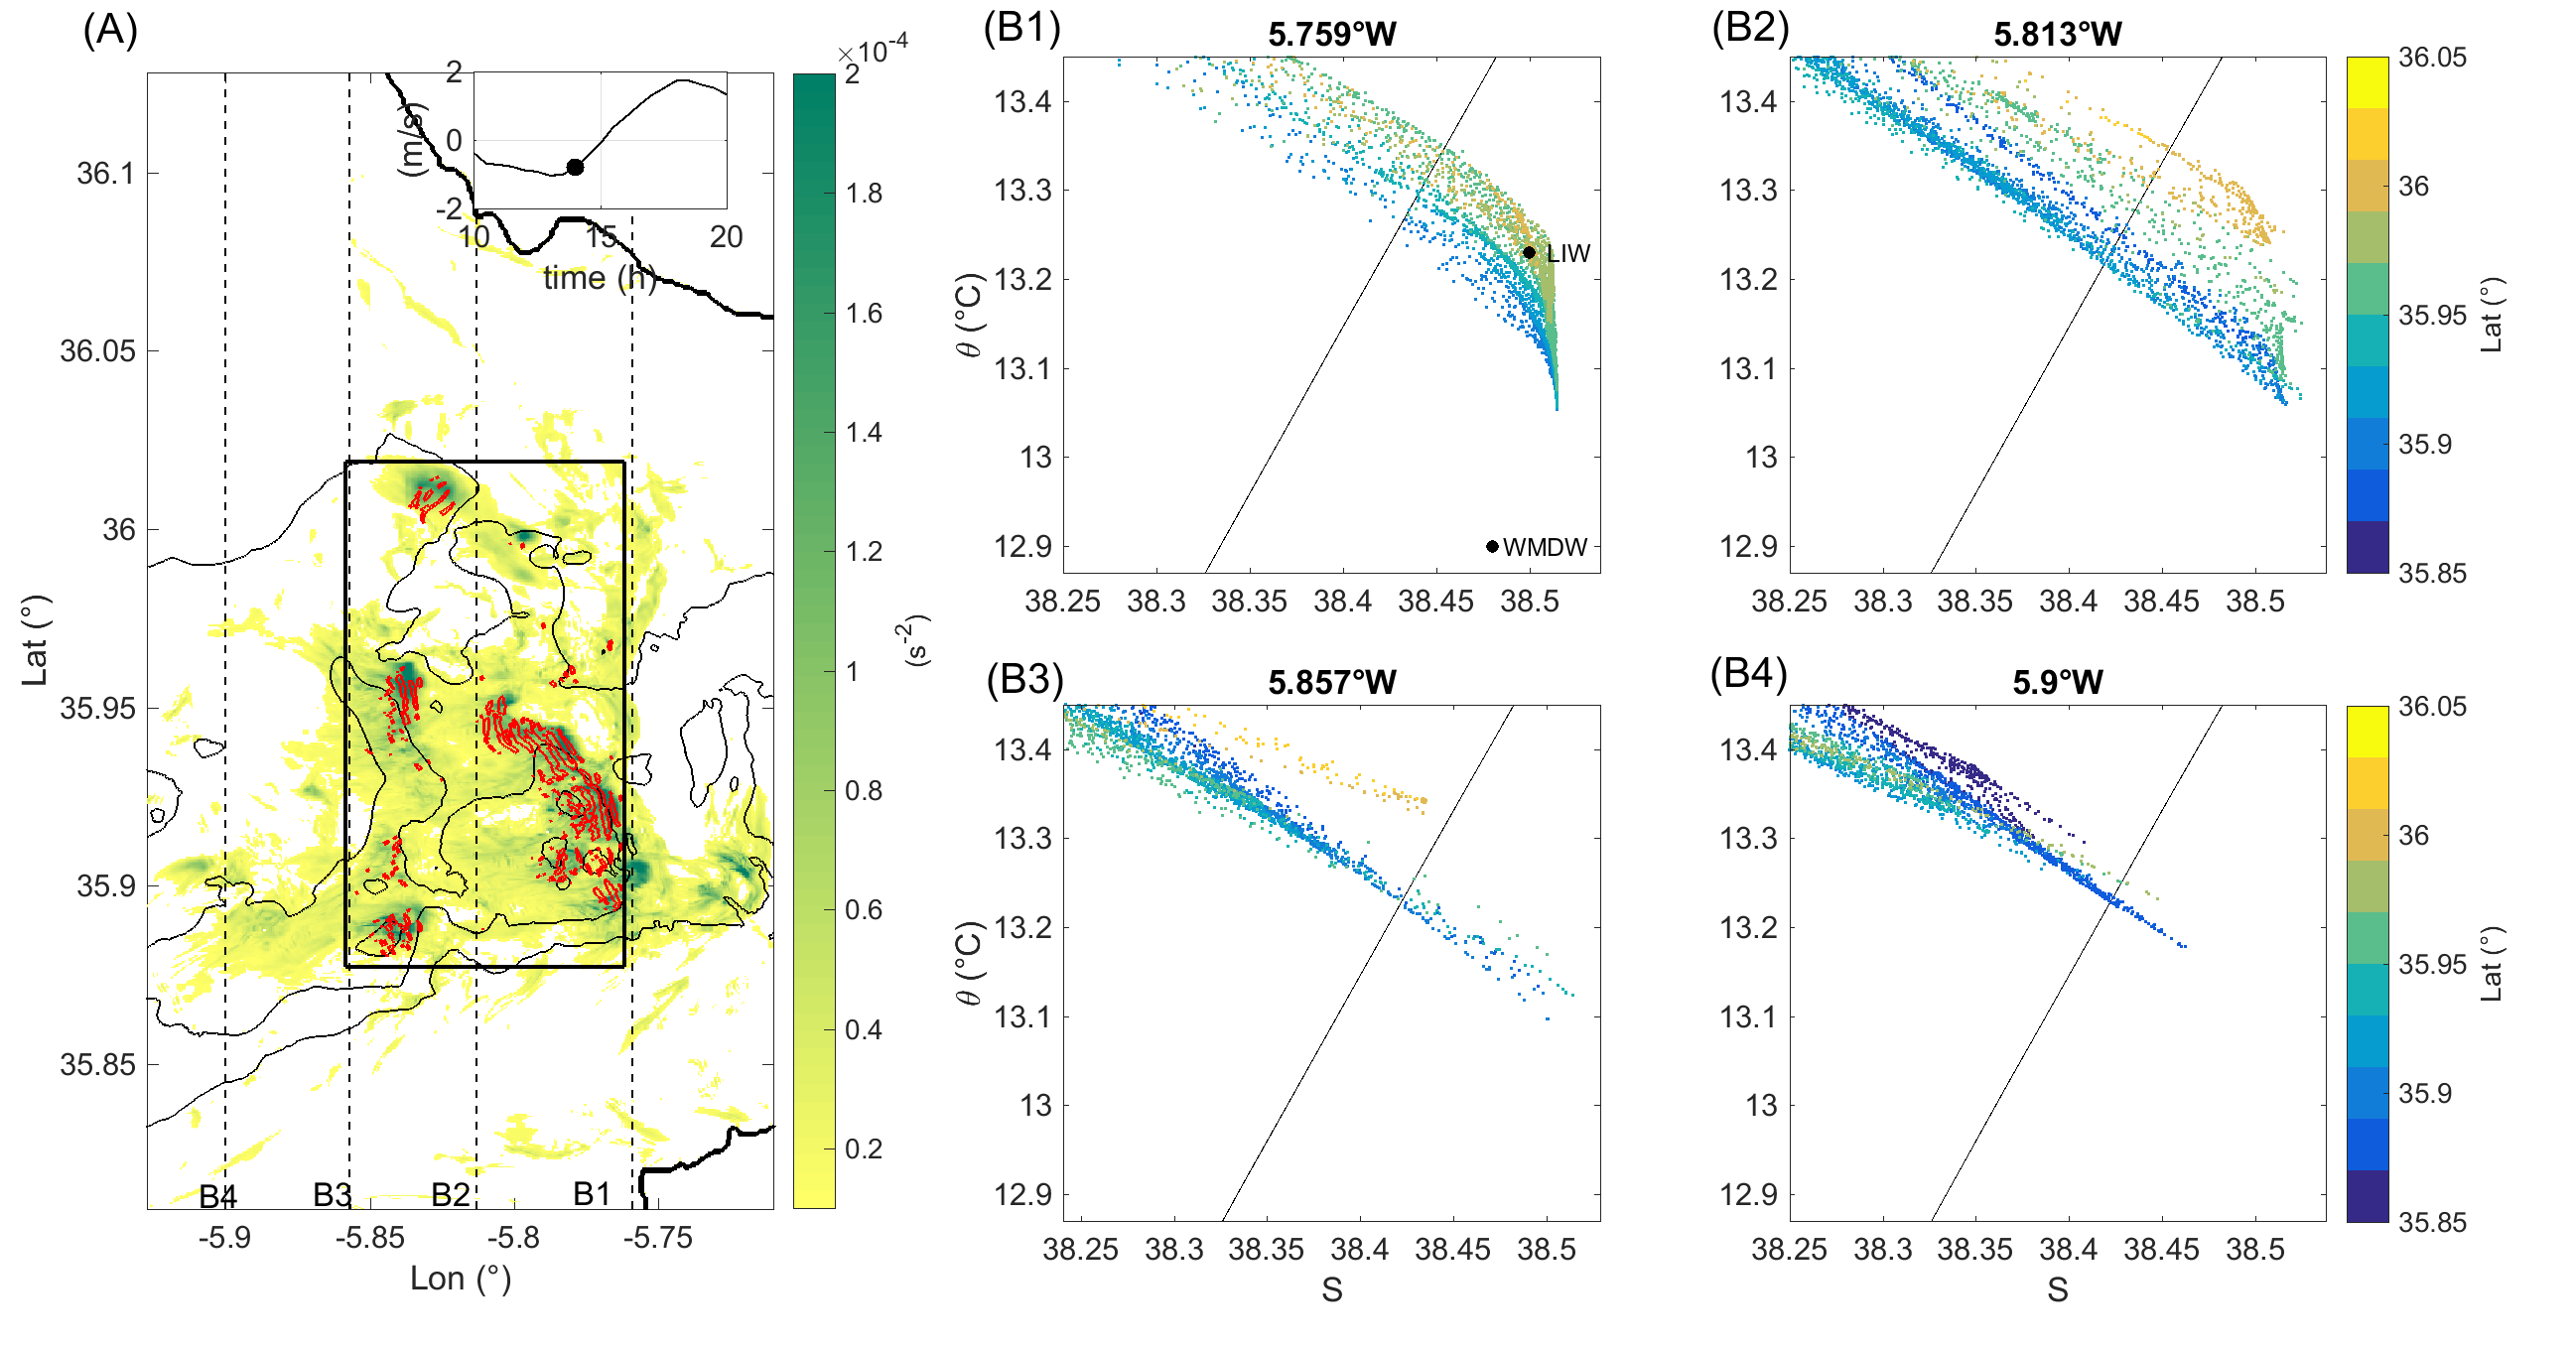
\includegraphics[width=\textwidth]{./GBR3D/TS_coupes_14H_VE2o.png}
 \caption {(a) Standard deviation of parameter Q over 30 mintues at t=14H in SimST (color) and trace of Q$=5$ from the high-frequency EOF of SVD performed in the rectangular black box during the outflow period. Black dashed lines indicate the longitude at which T,S diagrams are plotted. (b,c,d,e) T,S diagrams, zoomed in on area of Mediterranean watermasses. (Mettre LETTRES, rajouer section plus au sud?)}
 \label{FigTSCS}
\end{figure}


Now looking at the singular vectors of SVD for outflows of different strength of barotropic tidal currents . Figure \ref{FigEOFMIV}.a,b,c presents the EOF of parameter Q for the outflows of figures \ref{FigHCN},\ref{FigHCS},and\ref{FigHCI},along with vertical sections of salinity at the time of figure \ref{FigEOFMIV}d,e,f plotted along latitude 35.94$^\text{o}$N. Figure \ref{FigEOFMIV} g and h are histograms giving the height above seafloor and latitude of the grid points of the EOF for which Q$\geq 5e-5m^2/s^2$. On vertical sections, can see that the positive value of Q parameter are associated with billow structures of salinity that develop in the gravity current along the west slope of the Camarinal Sill. Those structures develop for each outflow case, but the wider distributions of height above sea floor and visualisation in the vertical section indicates the billows have greater radius in the hydraulic jumps cases, entraining more interfacial and atlantic waters into the mediterranean outflow. At this longitude where the instabilities are still developed, cores are not yet mixed in the simulation, can see as in the $\Theta$-S diagrams that the outflow is still heterogeneous.

The two hydraulic jump cases also differ, while instabilities develop along the same areas in no-jump and s-jump case, in the w-jump case the hydraulic jump and the start of the gravity current are co-localised at all latitude as seen in the vertical section, which adds a possible area of generation between 35.92$^\text{o}$N and 35.93$^\text{o}$N, down slope of the shallowest point of the sill where the flow of Mediterranean waters is not as strong for s-jump and no-jump cases.


\begin{figure}[!h]
% \centering
 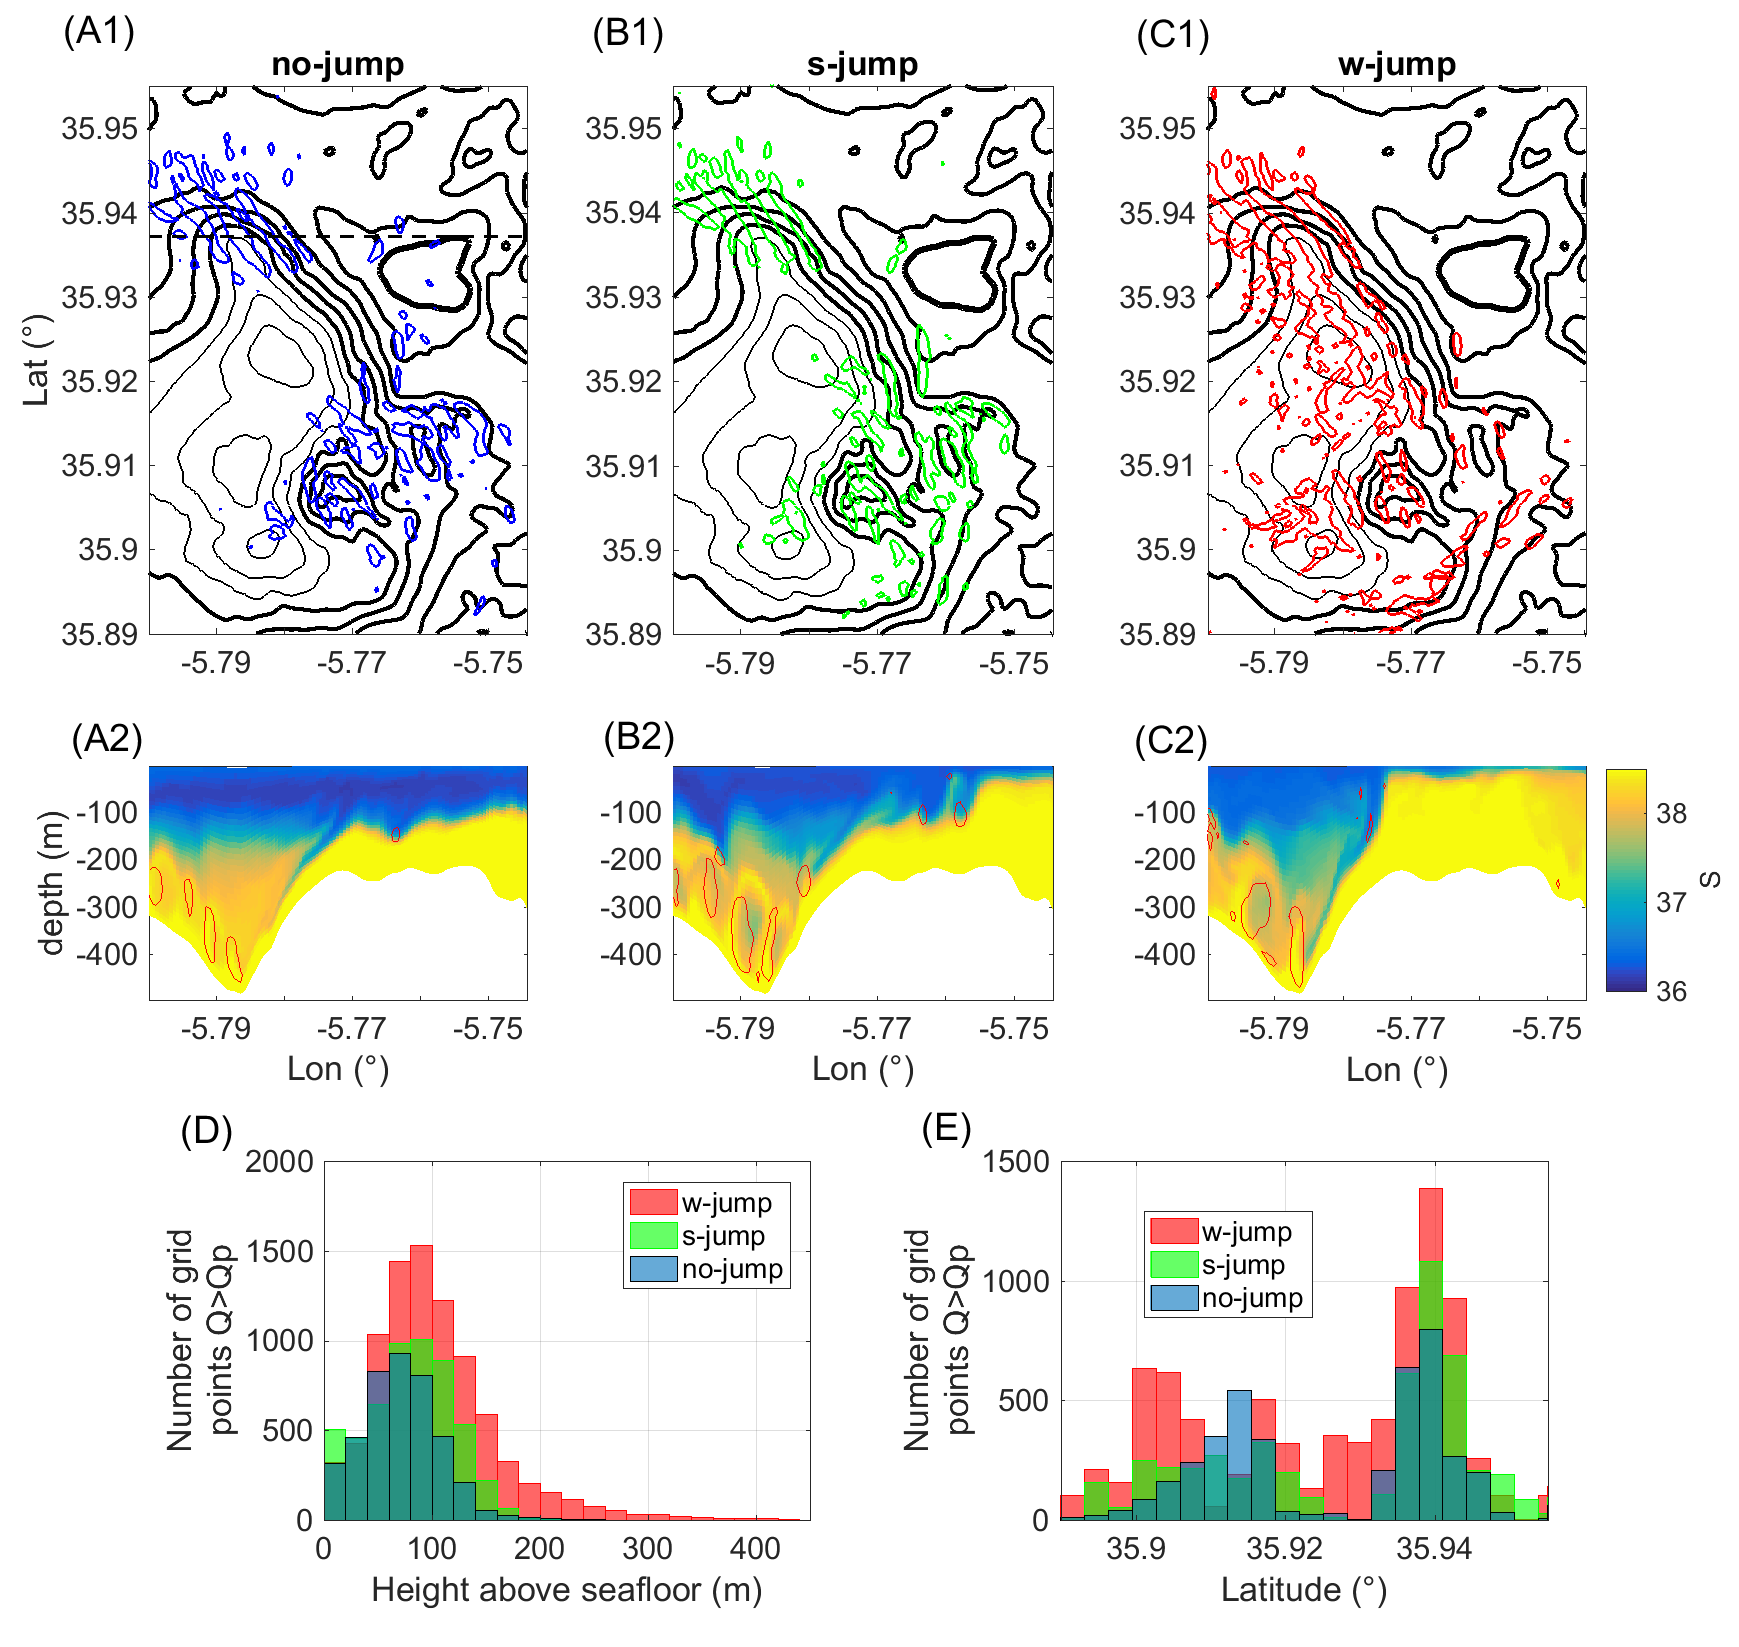
\includegraphics[width=\textwidth]{./GBR3D/EOF5_MIV_2D.png}
 \caption {(a,b,c) Contour of parameter Q$=5.10^{-5}$ in first high frequency EOF of SVD performed during outflow of figures \ref{FigHCN}.b,\ref{FigHCI} and \ref{FigHCS}.b respectively. and isobathes (black) (200m, thicker)  (250 to 450, thick) (500 to 600m, thin). (d,e,f) vertical section of salinity (color) and contour of Q-parameter $=5.10^{-5}$ at latitude $35.9372^\text{o}$ at the same time as figures \ref{FigHCN}.b,\ref{FigHCI} and \ref{FigHCS}.b respectively. (g) histogram of the height of the grid points of each EOF shown in a,b and c above the seafloor. (h) histogram of the latitude of the grid points of each EOF shown in a,b and c above the seafloar. }
 \label{FigEOFMIV}
\end{figure}


\subparagraph{Closure scheme}

Now look at four other simulations, three use Smagorinsky turbulent scheme with different coefficients. One is using GLS K-$\epsilon$. In figure \ref{Fig3Dsch}.a,c,e,g, vertical section of salinity during the first outflow at t$=$5h of simulation which is in a no-jump case, with Richardson gradient number $Ri$ and Q parameter indicated. $Ri$ is calculated from fields of density and velocity averaged over a half hour to filter out the propagating structures.

Figure \ref{Fig3Dsch}.b,d,f,h the averaged salinity in med (b,f) and atl layer(d,h),east (f,h) and west (b,d) of Camarinal Sill. Note that this is averaged value, as shown in figure \ref{FigTSCS} and can be seen in the vertical sections the outflow/med layer is not homogeneous at this longitude yet/those longitudes.


Looking at averaged layer salinities east of the Sill in figures \ref{Fig3Dsch} f,h, see that simulations SimIT-S001, SimIT-S01 and SimIT-Kep have same salinities for med layer, and can see some differences in atl layer punctually. , the simulations most different is SimIT-S1 that has a less salty med layer and a saltier atl layer. This is logical as with the enhanced mixing coefficient, more diffusion in the pycnocline between the two layers.

However, while the atl layer is again saltier west of the sill for SimIT-S1, so is the mediterranean layer, especially between 2 and 8 houyrs of simulation, which shouldn't be the case if only diffusion. Looking at the vertical section at 5 hours of simulation can see that instabilities develop for all of them. However, while can see that the area of $Ri=0.25$ starts at 5.77$^\text{o}$ for all four simulations, indicating shear instabilities could develop from this point in the gravity current, for simulation SimIT-S1 they start down slope of an intrusion of atlantic waters at 5.783$^\text{o}$W. While the other simulations, the salinity entrained by teh billows is from the altantic layer//contain less salty waters, ie the signal of atl surface water in the med outflow will be stronger in this simulation.

More atl waters incorporated for Kepsilon, for which the billows are not as developped, instabilitied less developed with smaller values of parameter Q (closer to a gravity current only?), and less salty outflow. This signal persists after $t=7h$ when the flow reverses and no more generation of instabilities, and in a lesser extent for SimIT-S1 for which the effect of more diffusion in the pycnocline may counteract with the injected med water.


While the width of the Med vein as it begins to go down slope of Camarinal as salty water is the same, in simulations 1 and 2 instabilities are earlier in the jump and bring more atl waters as the core or billows are advected down slope, resulting in more atl water being integrated to the med outflow at the passage of CS. 






\begin{figure}[!h]
% \centering
 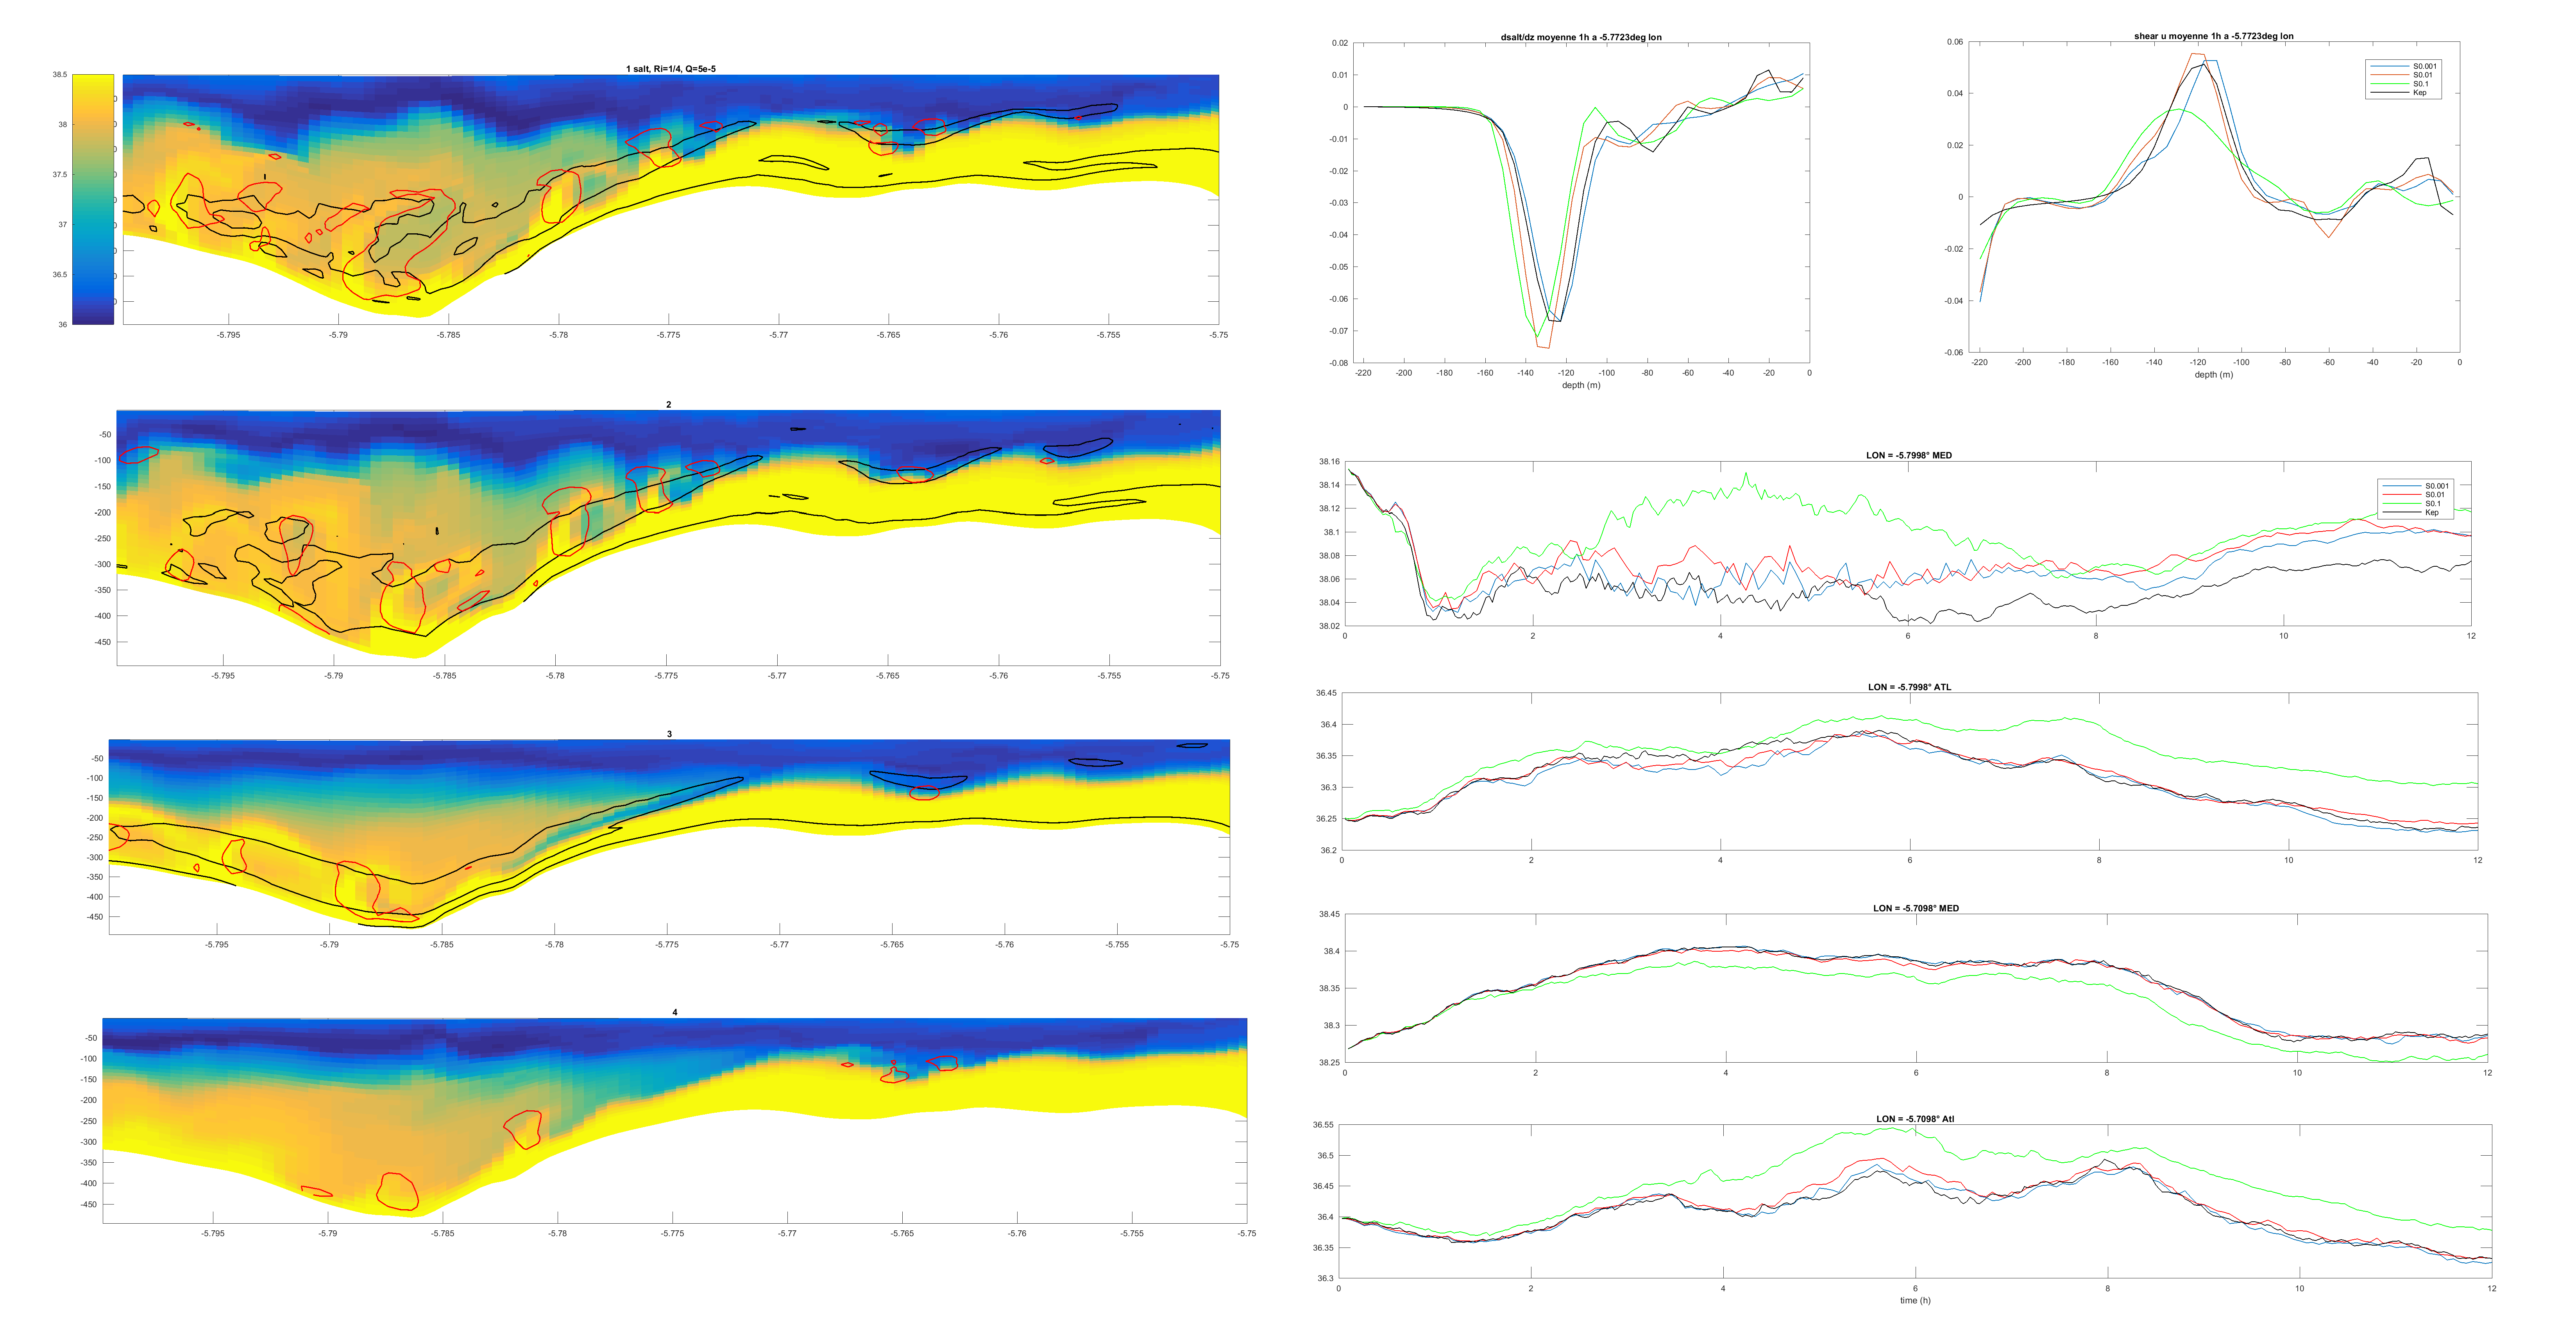
\includegraphics[width=\textwidth]{./GBR3D/Figsmago.png}
 \caption {Vertical section of salinity (color) and contour of $Q=5.10^{-5}$ (red) and Richardson gradient number $=025$ (black) at lat = $35.9372^o$ in simulations SimIT-S001,SimIT-S01,SimIT-S1 and SimIT-Kep IES at t=4h of simulation. time  (1:S0.001  2:S0.01  3:S0.1 4:Kep)(Rajouter une évolution de ubar!!! sur s0.001)}
 \label{Fig3Dsch}
\end{figure}

%-------------------------------------------------------------------------------------
\subsection{Conclusion}

Have looked into the variability in neap-spring tidal cycle of hydraulic control and other features in high resolution non hydrostatic simulation of the strait of Gibraltar.See no permanent supercritical flow across the simulations, only intermittent with the tidal cycle, with location and extension of the area of supercritical flow depending on the strength of the barotropic currents.

In outflow when both atl and med layers are critical, hydraulic jump, which position is either over the shallowest part of the sill, or over its western slope. This hydraulic jump evolves into train of solitary waves, as expected once hydraulic control is lost near high tide, that exits the strait into the Alboran Sea. Even for tidal cycle for which the flow over the sill is not critical and there is no formation of hydraulic jump, the non-linearity of the propagation of the barotropic tidal signal in the eastern part of the strait devolves into a less extended train of solitary waves propagating into the Alboran Sea.At each simulated tidal cycle, a cyclonic eddy is formed of the coast of Ceuta in the southern part of the eastern exit of the Strait. This eddy is advected by the flow in th Alboran Sea and interacts with the train of solitary waves, locally diffracting the waves.


Other feature present in simulations are the billows/shear instabilities developing in the lee of CS. In simulations, these billows are associated with high positive values of parameter Q that is used as proxy for their detection and analysis. The billows are generated at interface of med and atl waters and advected by the med outflow.   they are also present at secondary relief in tangier basin and at espartel sill. They are present during outflows of all intensity, but their repartition will change with intensity of tidal currents. They have a role in the way the med water is mixed, with changes of hydrological features of the med vein, and in simulation the way this mixing occurs is sensible to the dynamic of the instabilities that is piloted by the turbulent dissipation scheme.


 Can see that the configuration of the flow at CS, by being the first passage of the Med waters, will affect the hydrological properties of the Mediterranean outflow, first by the volume of med waters that can flow west of the sill at each outflow, second by how much Atlantic waters are being mixed into it.

However, it is important to note that simulation only represents the beginning of the mixing by turbulent processes, in particular, no secondary evolution of KH instabilities.


Moreover, The lack of atmospheric forcing probably means inaccuracies of features of the upper layer, especially circulation of the Atlantic layer in Tarifa Narrows where wind stress affects the upper layer. This could explain why have the baroclinic tide degenerate into an internal bore then a train of solitary waves for all inflows following a \textit{no-jump} outflow at CS, whereas observations indicate that in neap tide do not have solitary waves at each tidal cycle. Other processes could be affected like the formation of eddy at the exit of the Strait that occurs at the coast and its advection into Alboran that is probably influenced by the WAG.



\chapter{GBR2D}
\begin{itemize}
\item R\'esum\'e en français
\item Papier 2D (! Changer numero de page pour debut pdf !, et retirer biblio (avec en fin these....), mise en page verifier...(problème tableau 2))
\item Recap/clsion/transition français
\end{itemize}

\section{Resumé en français}
\begin{itemize}
\item blabla détroit Gibraltar, pourquoi choisi cette zone, résumé intro papier
\item mise en place configuration, résolution, non hydrostatique...
\item résultats : a bien solitons (aspect, KdV), controle hydraulique, voit des rouleaux = instabilités primaires (confirmation)
\end{itemize}

CE chapitre contient l'artcile "..." publié dans ... .CErtains des éléments de cet article, l'élaboration du processus de 
certaisn éléments d'analyse de cette configuration ont été ralisés entière ment ou au moins améliorés dans la première année de thèse, c'ets le cas de l'analyse en composante principake des instabilités primaire sdéveloppées...etc.


Une configuration numérique simple 2D est implémentée dans le détroit de Gibraltar avec le code communautaire CROCO dans sa version non-hydrostatique, non-Boussinesq (CROCO-NBQ). Cette configuration est peu coûteuse en temps de calcul et incorpore la bathymétrie le long de l'axe du détroit avec sa configuration de seuils (Farmer et Armi, 1988, programme \textit{Gibraltar Experiment}). Dans l'élaboration de cette configuration, une attention toute particulière a été apportée au rôle de la pseudo-force de Coriolis sur l'échange moyen simulé lors de l'initialisation par \textit{lock-exchange}.\\

LA simulation est initialisée par lock exhange, c'est à dire un profil type atl et med de part et d'autre du seuil de camarinal, point central du passage.LA marée est simulée par un courant barotrope à la frontière ouest. Dans une simulation où la rotation de la terre n'est pas rise en compte, mélange détruit stratification obtenue apres relâchement du lock exhange, en particulier la profondeur de l'interface où se propagent les solitons, suite au mélange intense par la marée interne.


Malgré les défauts inhérents à une représentation 2D-verticale (nécessairement limitée dynamiquement et non représentative des effets longitudinaux comme le contrôle dans le détroit de Tarifa), la configuration proposée permet de représenter de façon réaliste les mécanismes de \textit{fine échelle} dans le détroit à la fréquence de la marée barotrope : propagation des deux premiers modes d'ondes internes, contrôles hydrauliques aux seuils, ressaut hydraulique, et mélange turbulent. En particulier, les ondes internes de grande amplitude de mode 1 se propageant dans l'est du détroit sont caractérisées comme ondes solitaires (ou solitons) par comparaison avec le modèle analytique non-linéaire de Korteweig de Vries.\\

La modulation des phénomènes observés par divers paramètres (bathymétrie, intensité des courants de marée, hypothèse hydrostatique, résolution spatiale) est étudiée en détail. A haute résolution (environ 45 m), la relaxation de l'hypothèse non-hydrostatique est indispensable pour représenter les instabilités de cisaillement qui apparaissent dans le jet Méditerranéen, et qui constituent l'amorce de la cascade turbulente directe.



%%%%PAPIER 2D%%%%%%%%%%%%%%%%%%%%%%%%%%%%%%%%%%%%%%%%
%voir si faut mettre pdf envoye ou quoi.... mise en forme abstract, key words, auteurs...
%%% faut le mettre en section seul sans les plus petits titres...
%%numerotation...
%\newpage
%%%%%%%%%%%%%%%%%%%%%%%%%%%%%%%%%%%%%%%%%%%%%%%%%%%%%%%%%%%%%%%%%%%%%%%%%%%%
%   Manuscrit these
%%%%%%%%%%%%%%%%%%%%%%%%%%%%%%%%%%%%%%%%%%%%%%%%%%%%%%%%%%%%%%%%%%%%%%%%%%%

%%%%%%%%%%%%%%%%%%%%%%%%%%%%%%%%%%%%%%%%%%%%%%%%%%%%%%%%%%%%%%%%%%%%%%%%
\documentclass[a4paper,12pt,notitlepage]{report}
%%%%%%%%%%%%%%%%%%%%%%%%%%%%%%%%%%%%%%%%%%%%%%%%%%%%%%%%%%%%%%%%%%%%%%%%%%%

%%%%%%%%%%%%%%%%%%%%%%%%%%%%%%%%%%%%%%%%%%%%%%%%%%%%%%%%%%%%%%%%%%%%%%%%%%%
% Packages
%%%%%%%%%%%%%%%%%%%%%%%%%%%%%%%%%%%%%%%%%%%%%%%%%%%%%%%%%%%%%%%%%%%%%%%%%%%

\usepackage[a4paper,top=1.5cm,bottom=2cm,left=2.5cm,right=2.5cm,marginparwidth=1.75cm]{geometry}
\usepackage{graphicx} 
\usepackage[hidelinks]{hyperref} 
\usepackage{multirow} 
\usepackage{tabularx} 
\usepackage{color} 
\usepackage[fleqn]{amsmath}
\usepackage{amsfonts}
\usepackage{amssymb}
\usepackage{textcomp}
\usepackage{gensymb}
\usepackage{array}
\usepackage{amsxtra} 
\usepackage{wasysym} 
\usepackage{isomath} 
\usepackage{mathtools} 
\usepackage{txfonts} 
\usepackage{upgreek} 
\usepackage{enumerate} 
\usepackage{tensor} 
\usepackage{pifont} 
\usepackage{titlesec}
\usepackage[utf8x]{inputenc}
\usepackage[T1]{fontenc}
\usepackage{fancyhdr}
\usepackage{enumitem}
%\usepackage[colorlinks=true, allcolors=blue]{hyperref}
\usepackage{subcaption}
\usepackage[normalem]{ulem} %25/05 Barrer un texte.
\usepackage{caption}        %04/06
\usepackage{afterpage}      %04/6
\usepackage{geometry}       %05/06
%\usepackage{wrapfig}        %04/06
\usepackage{float}
%\usepackage[printfigures]{endfloat}
%\usepackage{endfloat}
%\usepackage{subfig}
%\usepackage{graphicx}
%package floatend
\usepackage{booktabs}
\usepackage{appendix}
%\usepackage{array, makecell}
%\renewcommand\theadfont{\bfseries}
%\usepackage{esint}
\usepackage{cancel}
%\usepackage{pdfpages}
%----------------------------------------------------------------------------
% Packages: uncomment to debug
%----------------------------------------------------------------------------
%\usepackage{refcheck}
%\renewcommand{\labelitemi}{\textbullet}

%----------------------------------------------------------------------------
% Packages: bibliography
%----------------------------------------------------------------------------
\usepackage[nottoc, notlof, notlot]{tocbibind}
%\usepackage[authoryear, round]{natbib}
\usepackage[authoryear]{natbib}
%\usepackage[frenchb]{babel}
%\usepackage{authblk}

%%%%%%%%%%%%%%%%%%%%%%%%%%%%%%%%%%%%%%%%%%%%%%%%%%%%%%%%%%%%%%%%%%%%%%%%%%%
% Definitions & commands
%%%%%%%%%%%%%%%%%%%%%%%%%%%%%%%%%%%%%%%%%%%%%%%%%%%%%%%%%%%%%%%%%%%%%%%%%%%

%----------------------------------------------------------------------------
% New operators
%----------------------------------------------------------------------------
\DeclareMathOperator{\cotan}{cotan}

%----------------------------------------------------------------------------
% New commands
%----------------------------------------------------------------------------
\newcommand{\nhi}[1]{%
	{\itshape \color{magenta} (NHI approx: {#1})}}
\newcommand{\hi}[1]{%
	{\itshape \color{cyan} (HI approx: {#1})}}

%----------------------------------------------------------------------------
\setlength\parindent{0pt}
%----------------------------------------------------------------------------

%----------------------------------------------------------------------------
% Colors...
%----------------------------------------------------------------------------
\definecolor{color-1}{rgb}{0.21,0.37,0.57}
\definecolor{color-2}{rgb}{0.31,0.51,0.74}

%----------------------------------------------------------------------------
\geometry{hmargin=2.5cm,vmargin=2.5cm} %marges
%----------------------------------------------------------------------------

\renewcommand{\thepage}{}
\renewcommand{\thepage}{\arabic{page}}

\newcommand\norm[1]{\left\lVert#1\right\rVert}

\numberwithin{equation}{section}


%%%%%%%%%%%%%%%%%%%%%%%%%%%%%%%%%%%%%%%%%%%%%%%%%%%%%%%%%%%%%%%%%%%%%%%%%%%%%
\begin{document}
%%%%%%%%%%%%%%%%%%%%%%%%%%%%%%%%%%%%%%%%%%%%%%%%%%%%%%%%%%%%%%%%%%%%%%%%%%%%%

\hypersetup{pdfborder=0 0 0}%----------------------------------------------------------------------------
% \ref with or without ( )
%----------------------------------------------------------------------------
\let\noparref\ref
\renewcommand{\ref}[1]{(\noparref{#1})}

\setcounter{tocdepth}{3}%1 juste 1 niveau sous-partie de chapitre

Inclure pdf page de titre

\newpage
\textbf{Avant-propos et remerciements}
\addcontentsline{toc}{section}{Avant-propos et remerciements}
\newpage
%%%%%%%%%%%%%%%%%%%%%%%%%%%%%%%%%%%%%%%%%%%%%%%%%%%%%%%%%%%%%%%%%%%%%%%%%%%%%
\tableofcontents

%%%%%%%%%%%%%%%%%%%%%%%%%%%%%%%%%%%%%%%%%%%%%%%%%%%%%%%%%%%%%%%%%%%%%%%%%%%%%

\newpage
\chapter{Introduction}
%\cite{BS84}
\citet{armi_1985}



%3/4 pages au moins en français (idem pour conclusion)
%\begin{itemize}
%\item fines échelles et leur rétroaction/structuration de circu générale
%\item choix région Gibraltar (Rencontre deux masses d'eaux, alimentation Méditerranée, outflow med)
%\item les fines échelles à Gibraltar (quels phénomènes (solitons, ressaut, etc))
%\item Outils de la thèse : num, obs (compagne,sat)
%\item état des lieux modélisation num fines échelles océaniques, problematique quantification mélange diapycnale
%\item plan
%\end{itemize}

Certains des éléments bibliographiques sont repris dans les introductions des différents chapitres, conçus comme des articles.

\section[Un voyage en \textit{Terra incognita}]{Un voyage en \textit{Terra incognita\footnote{\cite{scotti_large_2010}}}}
\subsection{Dynamique océanique : vers les fines échelles}
\label{subsection_intro1}
%(pose principes circu océanique, présente contexte des échelles généralement considérées en océanographie physique)

%La circulation globale océanique, pilotée par les vents et le flux de flottabilité, s'organise en un ensemble de courants de grande échelles (gyre, AMOC,...) qui en parallèle et en interaction avec la dynamique de l'atmosphère, transporte la chaleur. \\
\begin{figure}[!h]
  \centering
  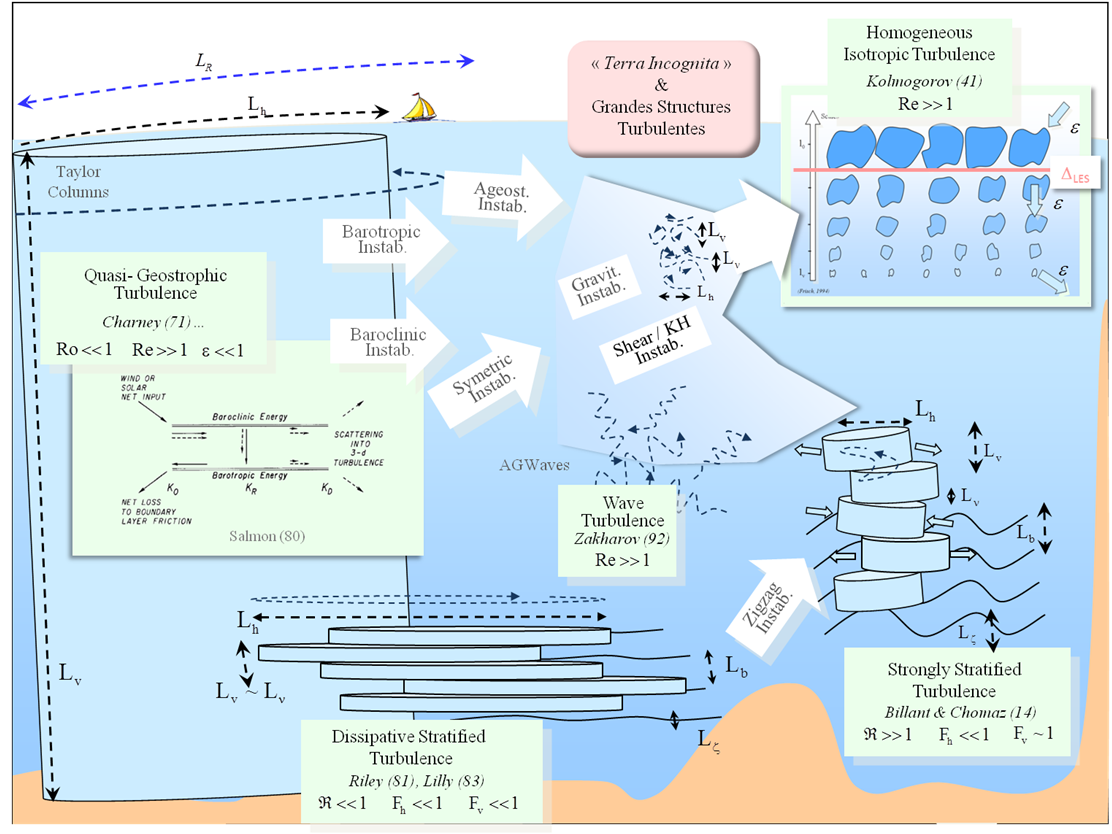
\includegraphics[width=0.8\textwidth]{./INTRO/Ocean_scales.png}
  \caption{\color{red}l'océan vu à travers ses cascades d'échelles, ses instabilités et ses principaux modèles de turbulence.\color{black}}
  \label{fig_ocean_scales}
\end{figure}
%\color{blue}
L'océan est soumis à/ mis en mouvements sous l'action de nombreux forçages par la pression atmosphérique, les marées astronomiques ou les flux de quantité de mouvement induits par le vent mais aussi par les flux de chaleur radiatifs ou par les flux de chaleur latente ou encore par les précipitations, les fleuves ou encore par évaporation... Ainsi présenté, l'océan peut donc être présenté comme un \textit{système dynamiquement ouvert}, l'ensemble des forçages auxquels il est soumis induisant un large spectre de processus dynamiques: houle, courants d'Ekman, upwelling ou downwelling, ondes de marée, marées internes, convection profonde, courants de gravité, panaches fluviaux... 


La dynamique de l'océan est variée, composée de processus dynamiques couvrant une large gamme autant spatiale que temporelle. La houle, les courants d'Ekman, les systèmes d'upwelling ou de downwelling, les ondes de marée, les marées internes, la convection profonde, les courants de gravité, ou encore les panaches fluviaux, 

, composée d'une large gamme de processus aux extensions géographiques 


%d'un large spectre de processus, on peut citer la houle, les courants d'Ekman, les systèmes d'upwelling ou de downwelling, les ondes de marée, les marées internes, la convection profonde, les courants de gravité, ou encore les panaches fluviaux... 

L'océan ne se résume toutefois pas à une somme de processus "forcés" dont la combinaison linéaire suffirait à expliquer sa dynamique propre. Ces processus interagissent en effet entre eux induisant d'importants \textit {mécanismes de transferts} entre les différentes gammes d'échelles spatiales et temporelles. Lorsque ces transferts prennent une forme cohérente dans quelques régions spécifiques du spectre, on parle de \textit{cascades d'échelles}. Les mécanismes débouchant sur ces transferts sont quant-à eux généralement associés à des \textit{instabilités dynamiques}.\\
\cite{salmon_baroclinic_1980} montrent par exemple qu'à méso-echelle\footnote{Région du spectre constitué d'échelles plus grande que le premier rayon de Rossby.} ces transferts s'organisent de façon cohérente sous la forme d'une \textit{cascade inverse} associée à des transferts énergétiques barotropes dirigés majoritairement vers les plus grandes échelles\footnote{Une telle cascade "inverse" est caractéristique de régimes de turbulence 2D.} alors que les transferts d'enstrophie\footnote{A l'image de l'énergie cinéatique cinétique pour la vitesse, l'enstrophie est définie comme la moitié du carré de la vorticité relative, i.e. du rotationnel de la vitesse.} sont quant à eux majoritairement dirigés vers les plus fines échelles. 
Les vents et les flux de chaleur induisent ainsi des structures dynamiques (baroclines) qui sont brisées lorsque l'écoulement devient instable \citep{vallis_atmospheric_2006}.
Les \textit{instabilités barotropes et baroclines} sont par conséquent au coeur de cette cascade dite inverse, elles rythment les transferts autour des rayons de Rossby\footnote{Échelle caractéristique de longueur caractérisant localement l'impact de la rotation du globe terrestre sur une colonne océanique de stratification donnée.} barotropes et baroclines dans les écoulements de mésoéchelles. On parle de régime de \textit{turbulence géostrophique} \citep{charney_geostrophic_1971} dans une région du spectre où stratification de la colonne d'eau et rotation du globe terrestre jouent \textit{in fine} des rôles prépondérants et sont associés à des équations de bilan équilibrées de quantité de mouvement. La cascade inverse demeure toutefois un modèle qualitatif fournissant une grille de lecture pour processus complexes et "non localisés" du le spectre océanique.\\
Des structures de sous-mésoéchelle reçoivent ainsi énergie et enstrophie et sont elles-aussi sujettes à un large éventail d'instabilités \citep{mcwilliams_submesoscale_2016}: instabilité agéostophique, symétrique, frontale, convective ou encore instabilités de cisaillement, instabilités baroclines dans la couche de mélange océanique, instabilités paramétriques des ondes internes... Dans cette région du spectre, l'impact de la rotation du globe terrestre est plus faible qu'à mésoéchelle mais la stratification contraint fortement la dynamique océanique débouchant sur des formes de turbulence dites "stratifiées": \textit{turbulence stratifiée dissipative}, \textit{turbulence fortement stratifiée}. l'instabilité "zig-zag" fait office de pont entre ces deux formes de turbulence).\\
Les myriades d'ondes de gravité internes et d'ondes de gravité de surface interagissent aussi au point de donner lieu à une forme particulière de turbulence: \textit{la turbulence d'onde}. Leur déferlement, leurs instabilités donnent généralement naissance à des "patchs turbulents" annoncés par l'apparition de grandes structures turbulentes.\\
En deçà de cette mésoéchelle (on parle de sous-mésoéchelle), prend naissance une autre cascade présentant une certaine cohérence, la \textit{cascade directe} ou cascade de Richardson au sein de laquelle l'énergie est transférée "directement" vers l'échelle de Kolmogorov au delà de laquelle la dissipation moléculaire est active. Si les théories décrivant les transferts à mésoéchelles ne permettent pas de routes directes vers la dissipation, les transferts de sous-mésoéchelle le permettent.
Les \textit{grandes structures turbulentes} marquent l'entrée de cette cascade directe, elles sont associées à des instabilités de cisaillement telles que les instabilités de Kelvin-Helmholtz. A \textit{micro-échelle}, le modèle de turbulence homogène et isotrope 3D décrit de façon simple cette cascade. Les échelles spatiales et temporelles des grandes structures turbulentes ne sont toutefois pas clairement définies: elles peuvent atteindre quelques dizaines de mètres au sein de la colonne d'eau mais peuvent aussi ne pas dépasser le mètre dans les couches de surface ou de fond.\\
Cascades d'échelles et modèles de turbulence décrivent ainsi des régions spécifiques du spectre spatio-temporel de l'océan qui présentent une certaine cohérence. Les divers types d'instabilités tissent quant-à elles des ponts entre ces régions. En toute rigueur, comprendre, expliquer, simuler (explicitement) ou modéliser (implicitement) le mélange turbulent, impliquent donc évidemment de représenter correctement l'ensemble du spectre océanique, ses transferts, ses cascades... Elle requière toutefois plus spécifiquement de reproduire précisément la cascade turbulente directe, i.e. le transfert "inertiel" d'énergie aboutissant à la région "dissipative" du spectre. Le point de départ de cette cascade n'est cependant pas clairement défini et varie aussi bien dans le temps que dans l'espace. Seule l'apparition souvent intermittente de grandes structures turbulentes permet de localiser spatialement et temporellement ce point de départ.\\
%Les grandes structures turbulentes marquent donc l'entrée de la cascade directe menant à la dissipation moléculaire. Elles sont ainsi à l'origine d'une cascade débouchant sur une réorganisation irréversible, diabatique de la colonne d'eau et d'un redistribution des "traceurs" passifs ou actifs. Parmi ces "traceurs", la masse volumique joue un rôle particulier dans la dynamique océanique: les masses d'eau sont par exemple "transportées" le long des surfaces isopycnales et le contenu en vorticité potentielle entre deux de ces surfaces isopycnales se conserve au cours du temps.\\
A. Scotti \citep{scotti_large_2010}, dans une revue sur la modélisation de l'océan, conclut qu’avec l'étude des grandes structures turbulentes, s'ouvrent les portes de la \textit{terra incognita}. Il reprend ainsi la conclusion de J.C. Wyngaard \citep{wyngaard_toward_2004} rédigée quelques années auparavant pour l'atmosphère. Cette terre inconnue, souvent aussi qualifiée de "zone grise" abritant les \textit{fines échelles océaniques}, est plus largement considérée comme la région particulièrement mal connue du spectre océanique dans laquelle la dynamique peut localement et temporairement basculer d'un équilibre simple entre un nombre limité de processus vers une dynamique non-linéaire complexe induisant une cascade d'instabilités dynamiques (directe) aboutissant à la dissipation moléculaire. 
\color{black}
%Cependant, l'océan (tout comme l'atmosphère) a un écoulement turbulent, c'est-à-dire chaotique et non-linéaire/ constitué d'une intéraction d'échelle.
%...
%Cette turbulence se manifeste en la décomposition des structures de grande échelles/synoptiques en des champs de plus petite structures/structures de plus en plus petites (transiant?) en intéractions les unes avec les autres (tourbillons, etc). Ainsi l'étude de l'océan peut se faire à bien des échelles spatiales et temporelles
%Ce manuscrit de thèse porte sur l'étude d'une dynamique dite de 'fine échelle', sur les processus / phénomènes océaniques . Il s'agira 
\color{blue}
\subsection{Rétroactions}
\label{subsection_retroactions}
Le mélange peut ainsi être présenté comme l'aboutissement de transferts et de cascades plus ou moins cohérentes mais quoiqu'il en soit très hétérogènes et intermittentes. Il ne constitue toutefois pas un puits sans fond ou un aller sans retour. Les flux diapycnaux modifient en effet les masses d'eau, la dissipation visqueuse qui "injecte" de la vorticité potentielle\footnote{La vorticité potentielle est une quantité, une substance d'après \cite{haynes_conservation_1990}, essentielle dans la description des écoulements stratifiés et en rotation qui est conservée par advection} près du fond... et constituent donc autant d'exemples de retroaction sur la grande échelle.\\
\cite{penney_2020} ont montré que le mélange était finalement capable de structurer les plus grandes échelles en mettant en évidence l'apparition à plus grande échelle de relations linéaires entre la masse volumique et les traceurs passifs qu'ils simulent.\\
La région du détroit de Gibraltar séparant la mer Méditerranée de l'océan Atlantique est à ce titre tout à fait exemplaire. Les masses d'eau méditerranéennes et atlantiques s'y croisent de façon tout aussi éphémère que brutale. Le mélange de ces deux masses d'eau induit par les fortes amplitudes de marée modifient in fine la salinité ou la quantité de mouvement de ces masses d'eau exerçant un contrôle sur la dynamique de l'ensemble du bassin Méditerranéen \citep{armi_1988}, scellant en quelques sortes le régime dynamique de l'ensemble du bassin et fixant vraisemblablement le contenu en vorticité potentielle du jet méditerranéen en Atlantique Nord.\\
La dissipation turbulente exerce donc une rétroaction sur les plus grandes échelles du spectre océanique: elle  structure les masses d'eau mais aussi la circulation océanique.
\color{black}
%(Revient plus en détail sur la turbulence, cas où mot est utilisé (turbulence géostrophique? vs cascade turbulente))
%Turbulence de mésoéchelle (instabilité barocline), ici on s'intéresse au début de la cascade turbulente directe définie par Kolmogorov. Les 2 sont similaires en ce qu'elles concernent le transfert d'énergie vers de plus fines échelles. Pour le cas de la turbulence de fine échelle, // mais va aussi aboutir à structuration de l'écoulement en lui-même. (La conservation de la vorticité potentielle (PV) peut agir comme un effet structurant de jet/courants...//méandres d'un jet / courant structurés par la conservation de la vorticité potentielle... PV générée par diabatic processes (in boundary layers?)...

%Cascade inverse???

\subsection{Le détroit de Gibraltar}
%(intérêt de la zone en vu du blabla précédent)
\color{blue}
Les talus continentaux, dorsales océaniques, les monts sous-marins isolés et autres détroits sont autant d'accidents bathymétriques qui canalisent, perturbent, modifient la circulation générale des masses d'eau océaniques et plus généralement la dynamique de l'océan. Les accidents bathymétriques sont localement le siège de régimes de couches limites particuliers entraînant quasi-systématiquement l'apparition de structures turbulentes très localisées spatialement et ouvrant ainsi les portes de la "terra incognita".\\
Le détroit de Gibraltar déjà cité dans le paragraphe précédent (\S \noparref{subsection_retroactions}) comme exemple de région abritant des processus de fine échelle structurant la dynamique océanique de grande échelle, constitue l'archétype de l'accident topographique contraignant fortement la dynamique océanique. Il est en effet le lieu de passage obligé des échanges entre les bassins méditerranéens et atlantiques nord.\\
\color{red}
Je te laisse compléter avec une présentation de la dynamique de cette région : marée + circulation générale => ressaut + ISW +... fort mélange.\\
\color{blue}
La dissipation turbulente est répartie de façon très hétérogène dans la colonne d'eau océanique, souvent préférentiellement dans les couches de surface et de fond et généralement sous la forme d'évènements intermittents (on parle de bouffées turbulentes). Ces caractéristiques compliquent grandement sa localisation et sa quantification même si son impact sur la circulation générale est maintenant reconnu et décrit de façon très qualitative \cite{de_lavergne_abyssal_2017}. La région du détroit de Gibraltar offre donc un terrain d'étude particulièrement pertinent pour qui souhaite étudier cette dissipation turbulente et ses rétroactions puisque les bouffées turbulentes semblent devoir être associées aux régimes dynamiques présentant de fortes amplitudes de marée (donc facilement localisables dans le temps) et au dessus des principaux seuils parsemant le détroit (donc facilement localisables géographiquement cette fois).\\
Le choix du détroit de Gibraltar comme région d'étude privilégiée pour mes travaux de doctorat se justifie donc à plusieurs titres. Elle est particulièrement adaptée pour une première exploration en \textit{terra incognita} puisque quelques portes ouvrant une voie vers cette terre inconnue semblent y être facilement localisables: les grandes structures turbulents peuvent être un peu plus facilement localisables, observables et donc simulées explicitement de façon numérique. Le détroit de Gibraltar est de plus une région de choix pour mieux appréhender l'impact (la rétroaction) que pourrait avoir la dissipation turbulente sur la circulation générale dans les bassins méditerranéens et nord-atlantiques: il s'agit donc d'une région de choix pour étudier comment cette dissipation peut structurer une dynamique à beaucoup plus grande échelle.
\color{black}

\color{blue}
\section{Une exploration des fines échelles océaniques}
%\color{red}
%(verrous puis objectif)
\subsection{Définir cette région du spectre océanique}
Objet central de mes travaux de doctorat, les \textit{fines échelles} océaniques doivent en premier lieu être clairement définies. Jusqu'ici, ces fines échelles ont plus spécifiquement été associées dans notre introduction (\S \noparref{subsection_intro1}) à la région du spectre océanique identifiée comme \textit{Terra incognita}.\\
Les fines échelles sont donc par la suite définies comme les échelles spatiales et temporelles de l'ensemble des processus et autres mécanismes dynamiques de \textit{sous-mésoéchelle} \citep{mcwilliams_submesoscale_2016} auxquels s'ajoutent les grandes structures turbulentes ouvrant la voie à la cascade directe et marquant l'entrée de la \textit{micro-échelle}.
 \color{black}

\subsection{Se donner les outils et les moyens d'une telle exploration}
\color{blue}
Toute entrée dans un territoire inconnu tel que la \textit{terra incognita} est associée à la reconnaissance et à la levée d'un certain nombre de difficultés. Dans le cas présent, ces "difficultés" prennent la forme de véritables \textit{verrous} d'ordres dynamiques et numériques.
\subsubsection{Verrous dynamiques.}
Un certain nombre de "verrous" dynamiques peuvent être identifiés. Les grandes structures turbulentes dont il est en particulier question ici sont le résultat de diverses instabilités "primaires" peuplant la méso et la sous-méso-échelle océaniques: instabilités barotrope, barocline, symétrique, zig-zag, agéostrophique, paramétrique des ondes internes, etc... Ces mécanismes de déstabilisation peuvent être vus comme brisant des structures, des processus, des équilibres subtils régissant localement et de façon éphémère et intermittente la dynamique de l'océan. Leur exploration relève par conséquent plus d'une approche stochastique que purement déterministe.\\
Les grandes structures turbulentes constituent de plus des processus certes importants mais néanmoins indissociables des transferts d'échelles auxquels elles sont associées. Leur étude requiert donc la prise en compte simultanée de régions étendues du spectre océanique.\\
Ni les échelles spatiales ni les échelles temporelles des instabilités de cisaillement ne sont clairement identifiables à partir de grandeurs caractéristiques comme le peuvent être les rayons de Rossby pour la méso-échelle et les instabilités barotropes et baroclines.
\subsubsection{Verrous numériques.}
Les grandes structures turbulentes étaient traditionnellement l'apanage des modèles "sous-maille" dans les configurations océaniques côtières, régionales et à fortiori globales. N'étant par conséquent pas universels, ces modèles "sous-maille" rendent la simulation très dépendante du lieu et de la période étudiés: les "modèles de fermeture" doivent en effet être ajustés et confrontés à la réalité avec comme principal enjeu le choix du modèle et la détermination des paramètres physiques ou numériques qu’il inclut nécessairement. Si la réalisation de LES est envisageable et envisagées dans l’océan intérieur et peut donc être appuyée sur des modèles de turbulence plus universels et plus simple, elle demeure par contre hors d’atteinte dans les couches limites de surface et fond, régions dans lesquelles leurs échelles spatiales caractéristiques peuvent considérablement décroître pour être finalement de l'ordre du mètre. Des approches dites "zonales" doivent par conséquent être envisagées.
La simulation explicite des grandes structures turbulents engendre l'utilisation de grilles de calcul à très haute résolution sur des régions océaniques à priori relativement étendues. Elle requière donc un nouvel effort de réduction du coût de calcul. CROCO est en effet conçu et développé pour être un code efficace mais ce qu'il est aujourd'hui possible de simuler explicitement dans un détroit d'extension réduite doit être généralisé à des sous-bassins et à des plateaux continentaux de plus grande extension avec, très vraisemblablement, une résolution raffinée. Nous avons mené à bien une première étude de faisabilité au sein de notre petit groupe CROCO / LA débouchant sur le portage du code sur GPU sur des machines hétérogènes CPU / GPU. Le nécessaire travail d’optimisation des performances est désormais en conduit en très étroite collaboration avec les équipes INRIA. Le surcoût de calcul associé à la compressibilité et à la remise en cause de l'hypothèse hydrostatique a par exemple dors et déjà pu être effacé en déportant sur GPU l'intégration du mode rapide compressible.


\color{black}
\subsection{Simuler explicitement les fines échelles}
\color{blue}
Explorer numériquement les fines échelles océaniques implique de simuler explicitement les grandes structures turbulentes et l'on entre ainsi de plain-pied dans une approche numérique dite \textit{LES (pour \textit{Large Eddy Simulation})}.\\
La promesse d’une puissance de calcul pétaflopique puis exaflopique a, en théorie au moins, ouvert les portes de la simulation des grandes structures turbulentes (LES) pour l’océan et l’atmosphère. Les météorologues ont par exemple rapidement su tirer parti des moyens de calcul disponibles : des algorithmes dédiés ont vu le jour dès le début des années 2000 débouchant sur des codes numériques tels que WRF en version compressible ou Méso-NH en version anélastique. Ces deux types de codes permettent, chacun avec leurs spécificités, d’aborder la simulation de la cascade turbulente directe en représentant explicitement les plus grandes structures turbulentes dans l’atmosphère.
Les modèles océaniques n’ont pas été immédiatement en mesure de franchir ce cap de la LES en grande partie à cause de la présence d’une surface libre aux conséquences dynamiques multiples. La surface libre rend en particulier plus complexe la relaxation de l’hypothèse hydrostatique. Dans la foulée de l’ANR COMMODO rassemblant au milieu des années 2010 l’ensemble des équipes françaises travaillant sur la modélisation de l’océan, les équipes de recherche en océanographie dynamique et en mathématiques partenaires du projet CROCO se sont associées pour développer une nouvelle génération de codes capables d'explorer la "Terra Incognita". Un Groupement de Recherche éponyme est né associant l’université de Toulouse et les principaux organismes de recherche en informatique et en océanographie français: l’IRD, INRIA, le CNRS-INSU, l’IFREMER et le SHOM. En 2021, l’IRD a entériné la constitution d’un GdRi CROCO tourné vers nos partenaires au Sud.\\
Plusieurs pré-requis ont toutefois dû être satisfaits avant de lancer une exploration numérique des grandes structures turbulentes dans un contexte réaliste aussi complexe que celui du détroit de Gibraltar.
L'hypothèse hydrostatique, elle-aussi héritée du code ROMS, devait à minima être remise en cause en demeurant dans le contexte d'un océan à surface libre. Ceci fut chose en fait en relaxant aussi l'hypothèse de Boussinesq comme préconisée dans un contexte océanique par \cite{auclair_non-hydrostatic_2018}. L'héritage reçu du code américain ROMS \citep{shchepetkin_regional_2005} avait fait de CROCO un code particulièrement efficace dont le coeur numérique (son time-splitting, ses schémas numériques...) a été spécifiquement conçu pour limiter les coûts de calcul et l'utilisation de l'espace mémoire. Ce niveau de performance numérique a été maintenu pour son noyau numérique compressible et non-hydrostatique dans un contexte massivement parallèle.\\
De nouvelles recherches ont été entamées en parallèle de mes travaux de thèse pour d'une part porté sur le code sur une nouvelle génération de processeurs dits hétérogènes (associant CPU et GPU) et d'autre part permettre le raffinement local de la dynamique océanique par imbrication de configurations LES dans des maquettes numériques régionales très étendues. Les maquettes que j'ai développées ou co-développées dans le cadre de mes travaux de thèse ont servi de configuration-tests pour l'ensemble de ces développements transformant le détroit de Gibraltar en une région de démonstration.\\
\color{blue}
\subsection{Où l'on justifie une démarche scientifique pour cette exploration...}
\color{black}
Les années de thèse ont eu pour objectif de mettre en place outil sur une région particulièrement/// Simuler explicitement, observer, quantifier, pour explorer intéraction d'echelles sur spectre élargi


\section{Plan du manuscrit}




%Morceaux de intro GBR3D : 
%The amplitude of the exchange varies over timescales larger than the semi-diurnal tide. The lower frequencies (whether seasonal or inter-annual) are usually linked to atmospheric forcing over the Mediterranean \citep{sanchez-roman_2012}. The tidal eddy-fluxes have their own variability associated to the spring-tide cycle and to the monthly tides, with for example a greater depth and stronger shear during neap tides, but more intense mixing during spring tide \citep{naranjo_2014,vargas_2006}.\color{red}(enlever? sert à rien? que dans intro plus générale???)\color{black}


%Numerical models are discretized and have a treshold resolution under which phyisical pehomenons cannot be represented explicitely. Particularly, diffusion and ... processes,  among other parametrisations of processes like surface exchanges, radiation that occur at molecular or submolecular scales. Diffusion and dissipation are molecular in nature as a , energy flux, but more broadly speaking, dissipation is the transfer of energy from great scales to small scales. In a stratified fluid, this dissipation is accompagnied by mixing , ie a lewoering of potential energy, or more accurately and explained i paragraph ..., of the background potential energy.
%Broadly for oceanic (or more generally geophyisic?) models classification on DNS, LES, and RANS. DNS has molecular dissipation
%For the discussions simply coining as LES is not sufficient but need to precise LES in regard to which phenomenon. For exemplein chapoter ... of this manuscript, coined LES because primary instabilities of the flow. However, the primary instabilities that are known to exist at upper and lower boundaries of teh water column are not represented and are parametrized, so in regard to the dissipation those process not LES. 
%To this considerations, one must also not forget that the discretisation itself introduces numerical dissipation unless using centered schemes (computationnally impossible).



%\subparagraph{Conclusion générale/dans le manuscrit}
%Les simulations ... sont première LES maisblablablablabla (trad ce que avait dit...). Besoin outil diagnostique du mélange, chapitre prochain...





%%%%%%%%%%%%%%%%%%%%%%%%%%%%%%%%%%%%%%%%%%%%%%%%%%%%%%%%%%


\chapter{Mod\'elisation  Repr\'esentation de l'oc\'ean et de son m\'elange}
\begin{itemize}
\item conservation masses/qdm, discretisation numérique, échelles (RANS/LES(/DNS)), paramétrisation du mélange, fermeture turb (Smago/GLS...)
\item contenu en PV
\item definition BPE, eq d'évolution 'générale'
\item code CROCO (ou code CROCO en premisce de chap 3 GBR2D????(sinon parait cours?)GBR2D parle passage hydro a NBQ...)
\end{itemize}



\section{Résumé du chapitre en français}
Le présent chapitre présente de façon détaillée le \textit{modèle d'océan} utilisé dans le cadre de ma thèse pour simuler numériquement les grandes échelles turbulentes (ou LES$^{\noparref{LES}}$) dans la région du détroit de Gibraltar mais aussi, plus généralement, pour développer des modèles analytiques simplifiés de processus au service de cette approche numérique. Plusieurs sections du chapitre ont été intégrées à des publications acceptées \citep{hilt_2020}, \citep{auclair_modied_2021} ou en cours de rédaction  \citep{auclair_NBQ1_2021} mais aussi au rapport d'études du programme amont PROTEVS Gibraltar du SHOM \citep{auclair_modelisation_2019}. L'ensemble du chapitre est par conséquent rédigé en anglais.

Dans une première partie (\S \ref{section_prim_eq}) sont introduites les équations de conservations usuelles de l'océanographie physique, dont les équations de Navier-Stokes, point de départ du développement du \textit{modèle d'océan}. Le choix est ensuite fait de se placer dans le contexte d'une grille verticale curviligne qui permet d'épouser la forme des fonds marins et de suivre les mouvements de la surface libre de l'océan (dont un certain nombres de développements ont aussi présentés en annexe (\noparref{section_annexe2})). 
%Dans ce cadre, l'expression de l'évolution de l'énergie potentielle gravitationnelle (PE) et de ses sous-compartiments, énergie potentielle disponible (APE) et énergie potentielle de "background" (BPE), est développée dans un volume local d'océan (section \ref{section_PE_chap2}). En particulier, l'évolution de la BPE fait apparaître un terme source lié aux mouvements de la surface libre. Comme l'évolution de la BPE est lié au mélange diapycnale, la bonne expression de son bilan est impérative afin de faire des diagnostics de quantifications de mélange se basant sur cette méthode. %FA%

Dans la deuxième partie du chapitre (section \ref{section_croco}), est présenté le fonctionnement du code communautaire à cœur non-hydrostatique, compressible et à surface libre CROCO, basé sur le \textit{modèle d'océan} de la première partie. 
L'implémentation numérique de ce \textit{modèle d'océan} a demandé d'importants développements tant algorithmiques que numériques, développements qui ne peuvent être menés à bien s'ils miment directement la physique de l'océan. Parce qu'il est très général, ce \textit{modèle d'océan} peut réaliser la synthèse de processus dynamiques dans une gamme très étendue d'échelles spatio-temporelles depuis la circulation basse fréquence, jusqu'aux ondes acoustiques. Ce sont plus spécifiquement les plus fines échelles et les plus hautes fréquences qui peuvent imposer les plus fortes restrictions à l'approche numérique envisagée ; ce sont donc les processus associés et en particulier les processus ondulatoires acoustiques ou gravitaires qui ont été étudiés en priorité. 

%Ce \textit{modèle d'océan} est suffisamment général pour autoriser la représentation explicite d'une large gamme de processus allant des ondes et modes acoustiques dans un océan compressible aux structures turbulentes fondamentalement non-hydrostatiques de \textit{fine échelle} (associées par exemple à des instabilités de Kelvin-Helmholtz) en passant par des processus ondulatoires internes de grande amplitude (tels que les solitons).

J'ai participé à une partie des développements de CROCO durant ma thèse, sur le plan purement numérique tout d'abord, avec l'implémentation et l'évaluation de nouveaux schémas numériques dans un contexte pleinement réaliste et la mise en œuvre de stratégies originales pour la LES. Sur le plan de la dynamique océanique ensuite, avec la réalisation d'études de processus de fines échelles et l'étude des interactions complexes entre ces processus.

%Ce \textit{modèle d'océan} a de plus servi de base au développement dans le cadre de ma thèse de diagnostiques originaux dédiés à la simulation des grandes échelles turbulentes océaniques (LES) dans un contexte réaliste: évaluation quantitative du mélange turbulent (\S \noparref{chapter_bpe}), mise en évidence et caractérisation de ces structures, études de ressauts hydrauliques (\S \noparref{PartDiag3D})...

En parallèle des développements numériques et des travaux sur la dynamique de la région du détroit de Gibraltar menés dans le cadre de la présente thèse de doctorat, a été développé et publié un modèle analytique suffisamment général pour décrire la dispersion des ondes et des modes acoustiques, des ondes et des modes internes de gravité ou encore des ondes de gravité de surface \citep{auclair_modied_2021}. Le modèle analytique de dispersion a de plus été utilisé pour explorer la dynamique ondulatoire dans la région du détroit de Gibraltar.
J'ai participé et co-signé cette étude en support du développement numérique de CROCO, étude qui n'a pas été incluse dans le présent manuscrit.

Dans ce qui suit du présent chapitre, c'est l'anglais qui est utilisé pour les raisons évoquées précédemment.

%Dans une première partie, les équations analytiques servant de base à ce \textit{modèle d'océan} sont présentées (\noparref{section_prim_eq}), l'approche numérique choisie et co-développée pour le coeur numérique non-hydrostatique, compressible et à surface libre de CROCO est détaillée en partie \ref{section_croco}. Un certain nombre de développements sont enfin présentés dans les annexes (\noparref{section_annexe2}).


\section{A non-hydrostatic, compressible, free-surface ocean model}
\label{section_prim_eq}

%%%%%%%%%%%%%%%%%%%%%%%%%%%%%%%%%%%%%%%%%%%%%%%%%%%%%%%%%%%%%%%%%%%%%%%%%%%%%
 %----------------------------------------------------------------------------
 \subsection{Continuous free-surface compressible equations in z-coordinates}
 %----------------------------------------------------------------------------
\label{subsectiongenesystem}
\subsubsection{Model equations in conservative form}
Conservation of mass, conservation of momentum (Newton's second law of motion), conservation of total energy (first law of thermodynamics) and conservation of any tracers are the backbones of ocean dynamics. In the ocean, the conservation of mass can be written as a prognostic equation for density (written $\rho$), the conservation of momentum leads to prognostic equations for the three components of momentum (written $\rho \mathbf{v}$) and the conservation of total energy (or first law of thermodynamics) can be stated as a prognostic equation for potential temperature ($\theta$). The conservation of chemical species can then be expressed as a prognostic equation for salinity ($S$). These conservation equations consequently lead to the following general system of prognostic equations (expressed in flux form):
\begin{subequations}
 \begin{alignat}{2}
 \displaystyle
 \label{NS_a} 
 & \frac{\partial\rho}{\partial t} &&= - \mathbf{\nabla}\cdot(\rho \mathbf{v})\\[3mm]  
 \label{NS_b}
 & \frac{\partial \rho \mathbf{v}}{\partial t} 
	 &&= -\mathbf{\nabla}\cdot(\rho \mathbf{v}\otimes \mathbf{v}) 
	  \color{black} -2\rho\ \mathbf{\Omega}\ \times \ \mathbf{v} \color{black} -\mathbf{\nabla}p + 		
	\mathbf{\nabla}\cdot\left(
	\mu(\mathbf{\nabla}\mathbf{v}+\mathbf{\nabla}\mathbf{v}^{\ T})
 +\mu_2(\mathbf{\nabla}\cdot\mathbf{v})\ \mathbf{I}\ \right)
 +\rho \mathbf{g}\\
 %
 \label{NS_c}
 & \frac{\partial \rho \theta}{\partial t} &&=-\mathbf{\nabla}\cdot(\rho \theta\mathbf{v})
 +\mathbf{\nabla}\cdot\color{black}(\kappa_\theta\mathbf{\nabla}{\theta})\color{black}\\[3mm]
 %
 \label{NS_d}
 & \frac{\partial \rho S}{\partial t} &&=-\mathbf{\nabla}\cdot(\rho S\mathbf{v})
 +\mathbf{\nabla}\cdot\color{black}(\kappa_S\mathbf{\nabla}{S})\color{black}
 %
  \end{alignat}
\end{subequations}
with $\mu$, $\mu_2$, $\kappa_T$ and $\kappa_S$ respectively the dynamical and bulk viscosities and the thermal and salt diffusivities. $\mathbf{\Omega}$ is the earth instant rotation vector.
Assuming that variables are in thermodynamic equilibrium, the equation of state (EOS) can be formulated as a non-linear, diagnostic functional relation between temperature, salinity, density and (total) pressure (written $p$):
\begin{equation}
 \label{NS_e}
 \rho = \rho_{eos}[\theta,S,p]
\end{equation}

\subsubsection{Boundary conditions}
The position of the interface separating the ocean and the atmosphere must additionally be calculated and is introduced as a boundary condition. This can be achieved by stating that a salty-water particles that is just bellow this interface in the ocean, remains at the interface, leading to the surface kinematic relation:
\begin{equation}
  \displaystyle
  \label{NS_BC2}
  %\frac{\textrm{d}\zeta(\mathbf{x}_{\scriptscriptstyle H},t)}{\textrm{dt}}=w(\mathbf{x}_{\scriptscriptstyle H},z=\zeta)
  \frac{\partial \zeta}{\partial t}=w(\mathbf{x}_{\scriptscriptstyle H},z=\zeta)-\mathbf{v}_H(\mathbf{x}_{\scriptscriptstyle H},z=\zeta)\cdot\mathbf{\nabla}_H\zeta
\end{equation}
where $\zeta$ is the free-surface anomaly in the vicinity of the geoid and subscribe $H$ indicates that only the horizontal component is considered. Assuming then that ocean water cannot penetrate the ocean bottom (at depth $z=-H$):
\begin{equation}
 \displaystyle
 \label{NS_BC0}
  \mathbf{v}(\mathbf{x}_{\scriptscriptstyle H},z=-H)=\mathbf{0}
\end{equation}
Neglecting surface-tension pressure drop, the boundary condition for pressure at the surface of the ocean is given by:
\begin{equation}
 \displaystyle
 \label{NS_BC1}
  p(\mathbf{x}_{\scriptscriptstyle H},z=\zeta,t)= p_{atm}
\end{equation}
with $p_{atm}$ the atmospheric pressure above the surface of the ocean.
The resulting system of prognostic equations, diagnostic relations and boundary conditions leads to a non-linear problem whose main characteristics is the wild spectrum of dynamic processes involved (see for instance \cite{gill_atmosphere-ocean_1982} or \cite{vallis_atmospheric_2006}). Periodic processes such as ocean waves can give a comprehensive overview of the extension of space-time spectrum of transient processes which can propagate in the ocean and \cite{auclair_modied_2021} derive a compressible, free-surface, stratified model of two dispersion relations for wave-numbers and pulsation gathering acoustic, surface and internal waves and insisting on the modification of the dispersion of gravity (acoustic) waves by compressibility (gravity and stratification).

Formulated thus, the system of Navier-Stokes and conservation equations for a free-surface ocean can, at least in theory, be integrated straightforwardly. All variables but the pressure have their own prognostic equation and pressure can be diagnosed from the EOS \ref{NS_e}. Note that the system can be reformulated so that pressure is also given by a prognostic equation.

\subsubsection{Evolution of the density field}
For a linear approximation of the equation of state, a simple evolution equation of $\rho$ can be obtained as a combination of equations \ref{NS_c} and \ref{NS_d} leading to:
\begin{equation}
\displaystyle
\frac{d \rho}{d t}=
%\frac{\partial}{\partial x} \bigg(\kappa_\rho^h \frac{\partial \rho}{\partial x}\bigg\rvert_{tz}\bigg)_{tz}
%+ \frac{\partial}{\partial z} \bigg( \kappa \frac{\partial \rho}{\partial z}\bigg\rvert_{tx}\bigg)_{tx} 
 \mathbf{\nabla}\cdot\color{black}(\kappa_{\rho} \mathbf{\nabla}{\rho})
\label{eq_diff_cart}
\end{equation}
where $\kappa_{\rho}$ is the equivalent diffusivity of density.

 %----------------------------------------------------------------------------  
 %\subsection{Density and pressure decomposition}
 %----------------------------------------------------------------------------
 
\subsection{Terrain-following coordinates}
\label{subsection_scoord}

 %%%%%%%%%%%%%%%%%%%%%%%%%%%%%%%%%%%%%%%%%%%%%%%%%%%%%%%%%%%%%%%%%%%%%%%%%%%%%
\subsubsection{Definition}
%%%%%%%%%%%%%%%%%%%%%%%%%%%%%%%%%%%%%%%%%%%%%%%%%%%%%%%%%%%%%%%%%%%%%%%%%%%%%
The capacity of numerical models to mimic the evolution of global or regional oceanic circulation relies on horizontal and vertical definition of the grid on which the Navier-Stokes and conservation equations previously defined are solved and integrated in time.

Due to considerations of the representation of bathymetric features and free-surface evolutions, terrain-following coordinates, or S-coordinates, are chosen for the vertical discretisation. They are generally defined on generalized constant-$s$ surfaces with $s$ given by:
\begin{equation}
 \displaystyle
 s=s(x,y,z,t)=s(\mathbf{x},t)
\end{equation}
requiring thus that $s$ be a monotonic function of the vertical coordinate $z$:
\begin{equation}
 \displaystyle
 \frac{\partial s}{\partial z}\bigg\vert_{xyt}\ne 0
\end{equation}
$\partial s / \partial z$ is continuous and single-signed (either strictly positive or negative).

%%%%%%%%%%%%%%%%%%%%%%%%%%%%%%%%%%%%%%%%%%%%%%%%%%%%%%%%%%%%%%%%%%%%%%%%%%%%%
\subsubsection{Examples}
%%%%%%%%%%%%%%%%%%%%%%%%%%%%%%%%%%%%%%%%%%%%%%%%%%%%%%%%%%%%%%%%%%%%%%%%%%%%%
Several examples and comparisons on the choice of $s(\mathbf{x},t)$ are given in chapter 6 of \citet{griffies_fundamentals_2004}.
Following  \citet{shchepetkin_regional_2005},  less general $\sigma$-coordinates can be defined by:
\begin{equation}
 \displaystyle
 z(\mathbf{x},\sigma,t)=\sigma H(\mathbf{x_h})\quad or\quad z(\mathbf{x},\sigma,t)=\sigma(H(\mathbf{x_h})+\zeta(\mathbf{x_h},t))+\zeta(\mathbf{x_h},t)
\end{equation}
%or:
%\begin{equation}
% \displaystyle
% z(\mathbf{x},\sigma,t)=\sigma(H+\zeta)+\zeta
%\end{equation}
where $H(\mathbf{x_h})=H(\mathbf{x,y})$ is the bottom topography and $\zeta(\mathbf{x_h},t)$ the surface elevation anomaly. Its generalization to s-coordinates is defined by:
\begin{equation}
 \displaystyle
 z(\mathbf{x},s,t)=\mathcal{S}(s) H(\mathbf{x_h})
\end{equation}
which is currently written:
\begin{equation}
 \displaystyle
 z(\mathbf{x},\sigma,t)=\mathcal{S}(\sigma) H(\mathbf{x_h})
\end{equation}
and $S(\sigma)$ can be a non-linear function. Some current definitions are presented on the Wiki-Roms web-site \footnote{\url{https://www.myroms.org/wiki/Vertical_S-coordinate}}.


%%%%%%%%%%%%%%%%%%%%%%%%%%%%%%%%%%%%%%%%%%%%%%%%%%%%%%%%%%%%%%%%%%%%%%%%%%%%%
\subsubsection{Vertical velocities}
%%%%%%%%%%%%%%%%%%%%%%%%%%%%%%%%%%%%%%%%%%%%%%%%%%%%%%%%%%%%%%%%%%%%%%%%%%%%%
The definition of such a new vertical coordinate requires the derivation of the associated vertical velocity at the grid point. Using the coordinate transformation presented in section \ref{annexe_coordS} of appendix \ref{annexe_ocmod},  $w \equiv v_z$ can be decomposed as :
\begin{subequations}
  \begin{alignat}{2}
  \displaystyle 
	& v_z &&\equiv \frac{d z}{d t}\\
	& &&=\underbrace{\underbrace{\frac{\partial z}{\partial s}\bigg\rvert_{tx}}_{\equiv h} \frac{d s}{dt}}_{\equiv v_s}
	+\underbrace{\frac{\partial z}{\partial x}\bigg\rvert_{ts} \underbrace{\frac{d x}{dt}}_{\equiv u}
	+\frac{\partial z}{\partial t}\bigg\rvert_{xs} \underbrace{\frac{d t}{dt}}_{=1}}_{=\frac{dz}{dt}\big\rvert_{s}}\\[4mm]
	& &&=\frac{\partial z}{\partial s}\bigg\rvert_{tx} \frac{d s}{dt}
	+\frac{d z}{d t}\bigg\rvert_{s} \\[4mm]
	& &&=\ \ h \frac{d s}{dt}\quad
	+\frac{d z}{d t}\bigg\rvert_{s}\\[4mm]
	& &&=
	\ \ v_s 
	\qquad+\underbrace{\frac{\partial z}{\partial t}\bigg\rvert_{xs}
	+u \frac{\partial z}{\partial x}\bigg\rvert_{ts}}
	_{\frac{d z}{d t}\big\rvert_{s}=v_{\Sigma,z}}
  \end{alignat}
  \label{eq_vertvelcomp}
\end{subequations}
where:
\begin{equation}
	\displaystyle
	h\equiv\frac{\partial z}{\partial s}\bigg\rvert_{tx} \ \ \text{and} \ \
	v_s\equiv h\frac{d s}{d t}
\end{equation}

In other words, the vertical velocity is the composition of $v_{\Sigma,z}$ (the vertical component of the velocity of the constant-$s$ surface as it moves), and $v_s$ (the velocity through this same surface). An important aspect of this computation is that $v_s$ remains a velocity along the vertical axes since no change of direction of the axes is made.

%%%%%%%%%%%%%%%%%%%%%%%%%%%%%%%%%%%%%%%%%%%%%%%%%%%%%%%%%%%%%%%%%%%%%%%%%%%%%%
%\subsubsection{Vertical velocities in $"\sigma"$-coordinates}
%%%%%%%%%%%%%%%%%%%%%%%%%%%%%%%%%%%%%%%%%%%%%%%%%%%%%%%%%%%%%%%%%%%%%%%%%%%%%
In the more restrictive case where $\sigma$-coordinates are used:
% In $\sigma$-coordinates:
\begin{equation}
 \displaystyle
 \sigma=\frac{z-\zeta}{H+\zeta}
\end{equation}
and as a consequence:
\begin{equation}
 \displaystyle
 v_z=w=\mathbf{u}_z.\mathbf{v}
=\frac{dz}{dt}=\underbrace{(H+\zeta)\frac{d\sigma}{dt}}_{\equiv v_{\sigma}}
 +(\sigma-1)\frac{dH}{dt}
 +\sigma\frac{d\zeta}{dt}
\end{equation}
where in $\sigma$-coordinates:
\begin{equation}
 \displaystyle
v_{\sigma}=(H+\zeta)\frac{d\sigma}{dt}
\end{equation}

 \section{CROCO: a numerical implementation of the non-hydrostatic, compressible, free-surface \textit{ocean model}}
 \label{section_croco}
 
%----------------------------------------------------------------------------  
\subsection{Numerical implementation of the \textit{ocean model}}
%----------------------------------------------------------------------------
Ocean models whether dedicated to global, regional or even coastal scales are traditionally based on the Boussinesq, hydrostatic assumptions \citep{griffies_elements_2012,shchepetkin_regional_2005}. The present study is a step toward the explicit simulation of at least the largest turbulent eddies in a realistic context and, as a consequence, a non-hydrostatic numerical approach is required. \cite{Auclair2018} concluded that an efficient non-hydrostatic, free-surface, mode-splitting numerical model of the ocean could be designed relaxing also the Boussinesq approximation. Doing so, the authors chose to work with local equations and they do not solve for a 3D Poisson equation to diagnose total pressure. They consequently follow the choices made in meso-scale atmospheric modeling by \cite{skamarock_prototypes_2001}. The compressible (non-Boussinesq) approach is original in ocean modeling and in particular in free-surface, ocean modeling. Indeed \cite{marshall_finite-volume_1997} or \cite{auclair_non-hydrostatic_2011} chose to retain the Boussinesq assumption. A consequence of \cite{Auclair2018}'s choice is that the complete \textit{ocean model} presented in \S\ref{section_prim_eq} can be solved numerically.

The computing cost of such a non-hydrostatic, compressible, free-surface approach can quickly become prohibitive especially because the explicit modeling of fine scales requires high-resolution grids. Following the conclusions of the COMODO french community\footnote{COMODO gathered the french ocean modeling community. It was sponsored by the French ANR eponymous project (2011-2016).}, the compressible and free-surface algorithm developed by \cite{Auclair2018} has been implemented in the ROMS-AGRIF branch of the ROMS ocean models \citep{shchepetkin_regional_2005}. This choice was justified by the great efficiency of Shchepetkin's time-splitting and time-stepping and more generally by the experience accumulated in ROMS community during the last two decades.

The simulations of the strait of Gibraltar presented in chapters \ref{chapGBR2D} and \ref{chapGBR3D} were the very first realistic implementation of the non-hydrostatic, compressible, free-surface kernel of CROCO \citep{hilt_2020}.
\color{black}
%----------------------------------------------------------------------------  
\subsection{Time-splitting}
%----------------------------------------------------------------------------
\subsubsection{Dynamical time-scales}
Numerical constraints can conveniently be enumerated in terms of time-scales of dynamical "transfers" of tracer, pressure or velocity anomalies in the ocean. Advection, diffusion or radiation by gravity or acoustic waves are examples of such transfers. For a given length-scale (such as a model grid scale), maximum characteristic velocities can give  an order of magnitude for the most restrictive time-scales for each type of "transfer".\\
To derive the main characteristic length scales, the pressure and density anomalies are first conveniently defined with respect to the hydrostatic rest state leading to the pressure decomposition:
\begin{equation}
	\displaystyle
	\label{decompoP_0}
	p(\mathbf{x},t)=p_h(\mathbf{x},t)+\delta p(\mathbf{x},t)
\end{equation}
with $p_h(\mathbf{x},t)$ the hydrostatic pressure component and $\delta p(\mathbf{x},t)$ an anomaly. The former is defined by $\partial_z p_h=-\rho_h(\mathbf{x},t) g$ where $\rho_h(\mathbf{x},t)$ can be chosen as the slowly-varying, statically-stable field of density. Based on this pressure decomposition, a first-order Taylor expansion of the density field can be carried out :
\begin{equation}
  \displaystyle 
	\label{decompor_0}
  \rho(T,S,p)=\rho_{\theta S}(T,S,p_0)+\frac{p_h+\delta p-p_0}{c_s^2}+\mathcal{O}(\delta p^2)
\end{equation}
for a reference, slow component of pressure $p_0$ which is most often chosen different from the hydrostatic pressure in numerical models.
Numerical constraints relative to the various transfers of anomalies can basically be classified into three categories depending if they are associated to compressibility (acoustic waves..), surface-induced processes (surface gravity waves...) or internal-ocean (incompressible) processes (internal gravity waves, advection, diffusion, buoyancy-induced processes...). Orders of magnitude of maximum velocities in a deep ocean of each category are respectively given by $v[\delta p]\approx \mathcal{O}(1500\ m/s)$, $v[p_\zeta]\approx\sqrt{g H}\approx \mathcal{O}(100\ m/s)$ and $v[p_{int},\ ...]\approx \mathcal{O}(1\ m/s)$ leading to at least two spectral gaps in terms of velocities in the ocean:
\begin{equation}
	\displaystyle
	\label{velocityscales}
	v[p_{int},\ ...] \ll v[p_\zeta] \ll v[\delta p]
\end{equation} 
This hierarchy of velocity scales (and thus timescales for a fixed grid-scale) and the associated gaps constitute the basis to develop time-splitting approaches for numerical models of the ocean.
Under free-surface, Boussinesq and hydrostatic assumptions, the time-splitting procedure implemented in ROMS model \citep{shchepetkin_regional_2005} filters for instance acoustic and non-hydrostatic processes and takes advantage of the gap $v[p_{int},\ ...] \ll v[p_\zeta]$. It can be formulated as a decomposition of the pressure between a 2D surface-induced pressure-component (named external or barotropic-like component) $\bar{p}_h(\mathbf{x},t)$ and a 3D density-induced (internal or baroclinic-like) pressure-component $p_h'(\mathbf{x},t)$. 
The time-splitting approach for a more general free-surface, non-hydrostatic and compressible ocean can also be based on \ref{velocityscales}. The procedure is yet different from that used for hydrostatic ocean models. In the latter, coupling is based on the separation of the velocity field between a barotropic-like, depth-averaged component and a baroclinic-like anomaly. The faster, surface-induced component of the pressure force is integrated with a small time-step and after each integration sequence of the external mode, the depth-averaged component of the internal-mode velocity is forced to fit to the external-mode, depth-averaged velocity. Separating the "fast" and "slow" components of momentum in a compressible model to integrate them separately is not that simple and more importantly, it is not even necessary. The time-splitting procedure proposed in CROCO compressible kernel is indeed based on the splitting of the terms on the Right-Hand-Side (hereafter RHS) of the prognostic and diagnostic equations of the ocean model. Two coupled models (hereafter called the slow and fast numerical kernels) are then integrated in turn. The slow (respectively fast) kernel is advanced with a large (small) time-step computing explicitly slowly-varying (rapidly-varying) terms at the RHS and implicitly the remaining terms. A time-filtering procedure is additionally implemented to force both the slow and fast mode in a similar way as \citet{shchepetkin_regional_2005}.

\subsubsection{Pressure and density decomposition}
The splitting of the processes based on the magnitude of their time-scale relies essentially on a decomposition of the pressure and density fields. Following \cite{auclair_modied_2021}, the pressure decomposition \ref{decompoP_0} can be further developed for a free-surface ocean:
\begin{subequations}
  \begin{alignat}{2}
  % Pressure decomposition
  \displaystyle 
 \label{decompoP_fa}
  &p(\mathbf{x},t) &&= 
  \underbrace{p_{atm}
  (\mathbf{x}_{\scriptscriptstyle H},t)
  +g\int_z^{\zeta}\rho_{h}(\mathbf{x}_{\scriptscriptstyle H},z',t)\ dz'}_{p_h(\mathbf{x},t)}
  +\delta p(\mathbf{x},t)\\[3mm]
  \label{decompoP_f}
  & &&= \underbrace{\underbrace{p_{atm}
  (\mathbf{x}_{\scriptscriptstyle H},t)
  +\rho_0 g\left(\zeta(\mathbf{x}_{\scriptscriptstyle H},t)-z\right)}_{\bar{p}_h(\mathbf{x},t)}
  +\underbrace{g\int_z^{\zeta}{\left(\rho_{h}(\mathbf{x}_{\scriptscriptstyle H},z',t)-\rho_0\right)\ dz'}}
  _{p_h'(\mathbf{x},t)}}_{p_h(\mathbf{x},t)}
  +\delta p(\mathbf{x},t)
  \end{alignat}
\end{subequations}
where $\rho_0$ is a constant reference density. 
The Taylor expansion of density with respect to total pressure \ref{decompor_0} leads then to:
\begin{subequations}
  \begin{alignat}{2}
  % Pressure decomposition
  \displaystyle 
  % Density decomposition
  &\rho(\mathbf{x},t) &&=\rho_{\theta S}(\mathbf{x},t)
  +\underbrace{\frac{1}{c_s^{2}}\left(p_h(\mathbf{x},t)+\delta p(\mathbf{x},t)-p_0(\mathbf{x},t)\right)}_{(p(\mathbf{x},t)-p_0(\mathbf{x},t))/c_s^2} 
   +\, \mathrm{O}(p^2) \\[3mm]
  \label{decompor_f0}  
  & &&\approx\underbrace{\rho_h(\mathbf{x},t)+\rho_{nh}(\mathbf{x},t)
  +\frac{1}{c_s^{2}}\left(p_h(\mathbf{x},t)-p_0(\mathbf{x},t)\right)}_{\rho_{s}(\mathbf{x},t)}
  +\underbrace{\frac{\delta p(\mathbf{x},t)}{c_s^{2}}}_{\rho_f(\mathbf{x},t)}
  \end{alignat}
\end{subequations}
\noindent with $\partial p / \partial \rho|_\eta = c_s^2$ at constant entropy $\eta$, $\rho_{\theta S}=\rho_{eos}(\theta,\ S,\ p_0)$,   $\rho_{nh}=\rho_{\theta S}-\rho_h$, $\rho_s$ (and $\rho_f$) are respectively the components of the density field treated by the slow (fast) kernel (see bellow). This decomposition of the pressure and density fields clearly demonstrates, if necessary, the inextricable relationships between compressibility and hydrostaticity assumptions. 

 %----------------------------------------------------------------------------  
 \subsubsection{Slow vs fast components}
 %----------------------------------------------------------------------------
Based on the decomposition of the pressure and density fields (\noparref{decompoP_f}, \noparref{decompor_f0}), the terms at the RHS of the momentum equations can be splitted in two categories depending on the time-scales they are associated with: 
\begin{subequations}
\label{momsf}
   \begin{alignat}{2}
   \displaystyle
   %%%%%%%%%%%%%%%%%%%%%%%%%%%%%%%%%%%%%%%%%%%%%%
   % Momentum
   %%%%%%%%%%%%%%%%%%%%%%%%%%%%%%%%%%%%%%%%%%%%%%
   &\partial_t\rho\mathbf{v} &&= 
   \underbrace{-\mathbf{\nabla}.\left(\rho\mathbf{v}\otimes\mathbf{v}\right)
   %-2\rho\mathbf{\Omega}\wedge\mathbf{v}
   -\rho f\mathbf{u_z}\wedge\mathbf{v}
   -\mathbf\nabla(\int\limits_z^{\zeta}{(\rho_{s}-\rho_0)g\ dz'})
   +\mu\Delta\mathbf{v}}_{\mathbf{\Lambda}_{s}}\\
   & && \quad \underbrace{-\rho_0 g\mathbf\nabla\zeta
   -\mathbf\nabla{\delta p}
   -\rho f'\mathbf{u_y}\wedge\mathbf{v}
   +\rho\mathbf{g}
   +\mu_2\mathbf{\nabla}(\mathbf{\nabla}.\mathbf{v})}_{\mathbf{\Lambda}_{f}}
   \end{alignat}
\end{subequations}
Note that the Coriolis pseudo-force is itself splitted: the traditional component (with $f=2\Omega sin(\phi)$, $\mathbf{u}_z$ the vertical unit vector in Cartesian coordinates and $\phi$ the latitude) is integrated with the slow kernel whereas the non-traditional component (with $f'=2\Omega cos(\phi)$ and $\mathbf{u}_y$ the south-north horizontal unit vector in Cartesian coordinates). This latter component can indeed be associated with horizontal-axis rolls and is integrated with the fast kernel. The nonlinear advective terms are integrated with the slow kernel, i.e. a priori with a larger time-step and thus at a lower cost. Diffusion terms associated to dynamical (respectively bulk) viscosity are integrated with the slow (fast) kernel. The momentum equation \ref{momsf} can thus be rewritten in a compact, conservative form and in s-coordinates as:
\begin{subequations}
\begin{alignat}{3}
 \displaystyle
 &\partial_t\rho_s h_s\mathbf{v}_s   &&=\quad\Lambda_s  &&+\ll\Lambda_f\gg\\[3mm]
 &\partial_t\rho_f h_f\mathbf{v}_f &&=\ [[\Lambda_s]]   &&+\quad\Lambda_f
\end{alignat}
\end{subequations}
This splitting conserves basically the formulation of the horizontal momentum equations proposed in \cite{shchepetkin_regional_2005}: the length-scales of the processes and the fast-mode forcing are yet obviously different but the filtering procedure $\ll.\gg$ is the "flat" filter proposed by \cite{shchepetkin_regional_2005}. $[[.]]$ notation indicates the extrapolation in time of the slow-kernel terms to be used at the fast-kernel RHS (see \S \noparref{TimeSplit}).\\


%%%%%%%%%%%%%%%%%%%%%%%%%%%%%%%%%%%%%%%%%%%%%%%%%%%%%%%%%%%%%%%%%%%%%%%%%%%%%
\subsection{Time-stepping}
%%%%%%%%%%%%%%%%%%%%%%%%%%%%%%%%%%%%%%%%%%%%%%%%%%%%%%%%%%%%%%%%%%%%%%%%%%%%%
The time-splitting and time-stepping proposed in the following build both on \cite{shchepetkin_regional_2005} and on \cite{Auclair2018}.   \cite{shchepetkin_regional_2005}'s LFAM3\footnote{Leap-Frog Adams-Moulton 3 steps}, predictor-corrector time-stepping is indeed implemented in the slow kernel while a Forward-Backward (FB) scheme is used to integrate the fast-mode. The introduction of a compressible, non-hydrotatic kernel is taken from \cite{Auclair2018} and adapted to a two-mode implementation.

Figure \ref{ModelTS} shows the predictor-corrector implementation of the slow and fast kernels based on ROMS barotropic/baroclinic time-splitting. Both the time-splitting and the various time-stepping are summarized in Equations \ref{TimeSplit}.
\color{blue}
Note that in these equations and in the following, to simplify notations and to be coherent with CROCO's variables, s (for "slow") and f (for "fast") subscripts are indicated for right-most variable only: $\rho h \mathbf{v}_s=\rho_s h_s \mathbf{v}_s$ and $\rho h \mathbf{v}_f=\rho_f h_f \mathbf{v}_f$. This means that $\rho h \mathbf{v}$ is a CROCO variable. The decomposition of the density field into its fast and slow components is given by  \ref{decompor_f0}.\\
\color{black}
\begin{figure}[!h]
	\centering		
	\begin{subfigure}{1.0\linewidth}
		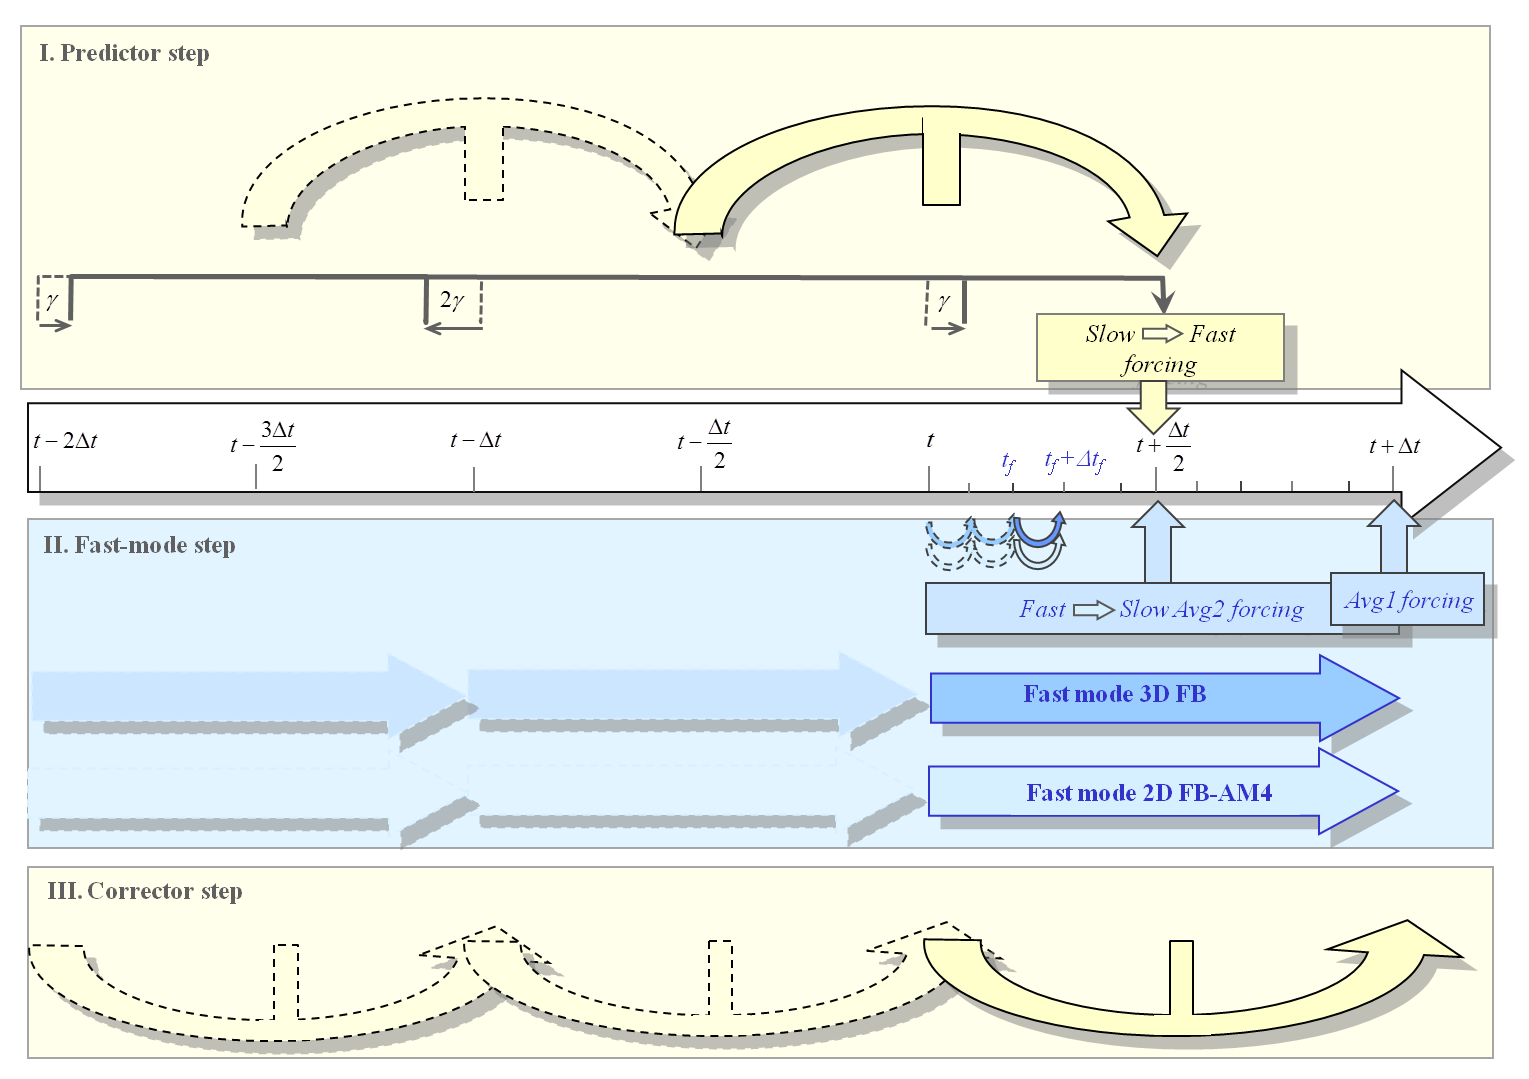
\includegraphics[width=1\linewidth]{CHAP2/Model_TS.png}
		\caption{}
	\end{subfigure}
\caption{ \textit{time-splitting and time-stepping of CROCO model with its non-hydrostatic, compressible (NBQ) kernel. Yellow (blue) background color: slow (fast) kernel. }}
	\label{ModelTS}
\end{figure}
%
\begin{table}
\begin{subequations}
\label{TimeSplit}
\begin{alignat}{3}
 \displaystyle
 %%%%%%%%%%%%%%%%%%%%%%%%%%%%%%%%%%%%%%%%%%%%%%%%%%%%%%%%%%%%%
 &\nonumber \textbf{I.a Time-interpolation: } t_s-\Delta t_s/2\\[0mm]
 %%%%%%%%%%%%%%%%%%%%%%%%%%%%%%%%%%%%%%%%%%%%%%%%%%%%%%%%%%%%%
 \label{TimeSplitIa1}
 &\enspace[\Theta] ^{n-\frac{1}{2}}=\alpha_{n-1}\Theta_s^{n-1}
 +\alpha_{n}\Theta_s^{n}\\[3mm]
 %%%%%%%%%%%%%%%%%%%%%%%%%%%%%%%%%%%%%%%%%%%%%%%%%%%%%%%%%%%%%
 &\nonumber \textbf{I.b Predictor step: } t_s+\Delta t_s/2\\[0mm]
 %%%%%%%%%%%%%%%%%%%%%%%%%%%%%%%%%%%%%%%%%%%%%%%%%%%%%%%%%%%%%
 \label{TimeSplitIb1}
 &\enspace\rho h\mathbf{v}_s^{n+\frac{1}{2}}=
 \rho h\mathbf{v}_s^{n-\frac{1}{2}}
 +\Delta t_s\left(\Lambda_{s,v}^{n}+<\Lambda_{f,v}>^n\right)\\[3mm]
 %
 \label{TimeSplitIb2}
 &\enspace\rho h(\theta_s,\ S_s)^{n+\frac{1}{2}}=
 \rho h(\theta_s,\ S_s)^{n-\frac{1}{2}}
 +\Delta t_s\Lambda_{s,(\theta,S)}^{n}\\[3mm]
 %
 \label{TimeSplitIb3}
 &\enspace\rho_s^{n+\frac{1}{2}}=\rho_{eos}\left(\theta_s^{n+\frac{1}{2}},\ S_s^{n+\frac{1}{2}},\ z_s^{n+\frac{1}{2}}\right)\\[3mm]
 %
 \label{TimeSplitIb4}
 &\enspace\partial_s\rho\omega_s^{n+\frac{1}{2}}=-\partial_t\rho h_s^{n+\frac{1}{2}}
 +\mathbf{\nabla}\cdot\rho h \mathbf{u}_s^{n+\frac{1}{2}}\\[3mm]
 %%%%%%%%%%%%%%%%%%%%%%%%%%%%%%%%%%%%%%%%%%%%%%%%%%%%%%%%%%%%%
 &\nonumber \textbf{I.c AB3-extrapolation: } t_s+\Delta t_s/2\\[0mm]
 %%%%%%%%%%%%%%%%%%%%%%%%%%%%%%%%%%%%%%%%%%%%%%%%%%%%%%%%%%%%%
 \label{TimeSplitIc1}
 &\enspace[[\Psi_s]]^{n+\frac{1}{2}}=
  \beta_{n-2}\Psi_s^{n-2}
 +\beta_{n-1}\Psi_s^{n-1}
 +\beta_{n}\Psi_s^{n}\\[2mm]
 %%%%%%%%%%%%%%%%%%%%%%%%%%%%%%%%%%%%%%%%%%%%%%%%%%%%%%%%%%%%%
 &\nonumber \textbf{II. Fast-mode steps: } t_f\in(t_s,\ t_s+\Delta t_s] \textit{ or } m\in[0,\ N_f)_\mathcal{N}\\[2mm]
 %%%%%%%%%%%%%%%%%%%%%%%%%%%%%%%%%%%%%%%%%%%%%%%%%%%%%%%%%%%%%
 \label{TimeSplitIIa}
 &\enspace\zeta_f^{m+1}=\zeta_f^{m}+\Delta t_f\left(
  w_{surf}^{m}-\mathbf{u}_{surf}^{m}.\mathbf{\nabla}\zeta^{m}\right)\\[2mm]
 %
 \label{TimeSplitIIb}
 &\enspace\rho h u_f^{m+1}=
 \rho h u_f^{m}
 +\Delta t_f\left(
  [[\Lambda_{s,u}]]^{n+\frac{1}{2}}
 -[[\overline{\Lambda_{s,u}}]]^{n+\frac{1}{2}}
 +\Lambda_{f,u}^{m}
% +\overline{\overline{\Lambda_{f,u}}}^{\ m}
 +\overline{\overline{\Lambda_{f,u}}}^{\ m}
 +\overline{\overline{\Lambda_{f,-\mathbf{\nabla}\zeta}}}^{\ m+1}
 \right)\\[2mm]
 %
 \label{TimeSplitIIc}
 &\enspace\overline{\overline{\rho h U}}_f^{\ m+1}=
 \overline{\overline{\rho h U}}_f^{\ m}
 +\Delta t_f\left(
 %[[\overline{\Lambda_{s,u}}]]^{n+\frac{1}{2}}+
 \overline{\Lambda_{f,u}^{m}}
 +\overline{\overline{\Lambda_{f,u}}}^{\ m}
 +\overline{\overline{\Lambda_{f,-\mathbf{\nabla}\zeta}}}^{\ m+1}
 \right)\\[0mm]
 %
 \label{TimeSplitIId}
 &\enspace\rho h w_f^{m+1}=
 \rho h w_f^{m}
 +\Delta t_f\left([[\Lambda_{s,w}]]^{n+\frac{1}{2}}
 +\Lambda_{f,w}^{m+1*}\right)\\[2mm]
 %
 \label{TimeSplitIIe}
 &\enspace\rho h_f^{m+1}=\rho h_f^{m}
 -\Delta t_f\left(
 [[\partial_t\rho h_s]]^{n+\frac{1}{2}}
 +\mathbf{\nabla}\cdot\{\rho h \mathbf{v}\}_f^{m+1}
 \right)\\[0mm]
 %
 \label{TimeSplitIIh}
 &\enspace m=N_f-1:\ \bar{\rho}\zeta_s^{n+1}
 =\bar{\rho}(H+\zeta_f)^{m}
 -\bar{\rho}H_s^{m+1}
 -\Delta t_f\mathbf{\nabla}\cdot\overline{\overline{\rho h\mathbf{u}}}^{\ m+1}\\[2mm]
 %
 \label{TimeSplitIIg}
 &\enspace \textit{Update\ grid:}\ \rho h_f^{m+1},\ z_f^{m+1}\\[2mm]
 %
 %%%%%%%%%%%%%%%%%%%%%%%%%%%%%%%%%%%%%%%%%%%%%%%%%%%%%%%%%%%%%
 &\nonumber \textbf{III.a Filtering: } t_s+\Delta t_s\ \textit{and}\ t_s+\Delta t_s/2\\[0mm]
 %%%%%%%%%%%%%%%%%%%%%%%%%%%%%%%%%%%%%%%%%%%%%%%%%%%%%%%%%%%%%
 \label{TimeSplitIIIa1}
 &\enspace<\Phi_f>^{n+1}=\Phi_f^{m=n+1}\\[0mm]
 \label{TimeSplitIIIa2}
 &\enspace\ll\Phi_f\gg^{n+\frac{1}{2}}=\frac{1}{N_f}\sum_{m=1}^{N_f}\Phi_f^{m}\\[2mm]
 %%%%%%%%%%%%%%%%%%%%%%%%%%%%%%%%%%%%%%%%%%%%%%%%%%%%%%%%%%%%%
 &\nonumber \textbf{III.b Corrector step: } t_s+\Delta t_s\\[0mm]
 %%%%%%%%%%%%%%%%%%%%%%%%%%%%%%%%%%%%%%%%%%%%%%%%%%%%%%%%%%%%%
 %
 \label{TimeSplitIIIb1}
 &\enspace\rho h\mathbf{v}_s^{n+1}=
 \rho h\mathbf{v}_s^{n}
 +\Delta t_s\left(\Lambda_s^{n+\frac{1}{2}*}
 +\ll\Lambda_f\gg^{n+\frac{1}{2}}\right)\\[0mm]
 %
 \label{TimeSplitIIIb2}
 &\enspace\partial_s\rho\omega_s^{n+1}=
 -\partial_{t\ }\rho h_s^{n+1}
 +\mathbf{\nabla}\cdot\rho h \mathbf{u}_s^{\ n+1}
 -\overline{\mathbf{\nabla}\cdot\rho h \mathbf{u}_s}^{\ n+1}
 -\overline{<\mathbf{\nabla}\cdot\rho h \mathbf{u}_s>}^{\ n+1}\\[2mm]
 %
 \label{TimeSplitIIIb3}
 &\enspace\rho h(\theta_s,\ S_s)^{n+1}=
 \rho h(\theta_s,\ S_s)^{n}
 +\Delta t_s\Lambda_{s,(\theta,S)}^{n+\frac{1}{2}*}\\[0mm]
 %
 \label{TimeSplitIIIb4}
 &\enspace\rho_s^{n+1}=\rho_{eos}\left(\theta_s^{n+1},\ S_s^{n+1},\ z_s^{n+1}\right)\\[0mm]
 %
 \label{TimeSplitIIIb5}
 &\enspace\rho h\mathbf{u}_s^{n+1}=\rho h\mathbf{u}_s^{n+1}
 -\overline{\rho h\mathbf{u}_s}^{\ n+1}
 +\overline{\rho h\mathbf{u}_f}^{\ m=N_f-1}
 %%%%%%%%%%%%%%%%%%%%%%%%%%%%%%%%%%%%%%%%%%%%%%%%%%%%%%%%%%%%%
\end{alignat}
\end{subequations}
\end{table}
Predictor (I), fast-kernel Forward-Backward (II) and Corrector (III) steps are shown in horizontal color bands on figure \ref{ModelTS} (yellow for the slow kernel, blue for the fast kernel). After time-interpolating slow-kernel variables to $t_s-\Delta t_s/2$ (step I.a, notation $[.]$), the slow kernel is advanced from $t_s-\Delta t_s/2$ to $t_s+\Delta t_s/2$ with a centered, leap-frog-like, time-stepping (step I.b). Then, to prepare the integration of the fast kernel, the slow-kernel RHS is extrapolated to $t_s+\Delta t_s/2$ based on an AB3 scheme using its previous evaluations at $t_s-2\Delta t_s$, $t_s-\Delta t_s$ and $t_s$ (step I.c, notation $[[.]]$). The fast kernel can in turn be advanced from $t_s$ to $t_s+\Delta t_s$ using a forward-backward like time-stepping (step II) with time-step $\Delta t_f$ satisfying  $N_f=\Delta t_s/\Delta t_f\in\mathcal{N}$. The vertical momentum equation can optionaly be integrated with semi-implicit scheme over the vertical direction.\\ 
The vertical grid is updated at each fast time-step \ref{TimeSplitIIg} but slow-kernel components of the RHS remain constant during the fast-kernel integration. At the last fast time-step, surface elevation displacement for the slow kernel can be recomputed to ensure perfect numerical coherence between the surface kinematic relation and depth-integrated mass conservation (\noparref{TimeSplitIIa} and \noparref{TimeSplitIIh}).\\
Further numerical details such as the values of the interpolation $(\alpha_n)$ or extrapolation $(\beta_n)$ coefficients, the expressions of the slow-kernel RHS terms $(\Lambda_s)$, the expressions of the fast-kernel surface-related pressure force terms $(\Lambda_{f,-\nabla\zeta})$,  the fast-kernel RHS remaining terms $(\Lambda_{f})$ or the implicit fast and slow-kernel RHS terms (indicated by an asterisk) can be found in CROCO dedicated manuals and publications.\\  
%The barotropic-like, depth-independent component is also integrated with the same time-step $\Delta t_f$ with a forward-backward scheme as in \cite{shchepetkin_regional_2005}. 
A major difference with the hydrostatic time-splitting is that the surface elevation displacement is given by the kinematic condition \ref{TimeSplitIIa} and not by the depth-integral of the mass conservation equation. Once the fast-kernel RHS and variables have been filtered both at $t_s+\Delta t_s$ and $t_s+\Delta t_s/2$ (step III.a, notations $<.>$ and $\ll.\gg$), the slow kernel is finally advanced from $t$ to  $t_s+\Delta t_s$ during the leap-frog-like Corrector step (III.b). A star following the time-index superscript indicates the use of an implicit numerical schemes.

Note that the 2D depth-averaged, barotropic-like, horizontal momentum equations (double over-bar notation) \ref{TimeSplitIIc} are advanced in the same way as in \cite{shchepetkin_regional_2005}. The result of this 2D integration is indeed used to correct both the horizontal momentum itself and the RHS of the horizontal momentum equation at Corrector step. It can also be used to require a perfect coherence of the surface elevation displacement and the depth-average transport (at machine precision) during the slow-mode integration.

\color{blue}
\section{Conclusion, discussion of the \textit{ocean model}}
In the present chapter, we proposed a rigorous framework (an "map") for our exploration of ocean \textit{fine scales} in \textit{Terra Incognita}. An analytical, terrain-following s-coordinate model for the conservation of mass, momentum, heat and tracers has first been proposed under general assumptions of a compressible, free-surface ocean (\S \noparref{section_prim_eq}). \\
%An original derivation (to our knowledge) of the evolution of the potential energy of a free-surface column of fluid has been carried out.\\%FA%
We then considered the numerical implementation of this general \textit{ocean model} (\S \noparref{section_croco}). After a consideration of the space-time scales potentially involved in the fine scale ocean dynamics, an original time-splitting has been detailed as an extension of \cite{shchepetkin_regional_2005}'s barotropic/baroclinic time-splitting. It is also a restriction to a two-mode time-splitting of \cite{Auclair2018}'s three-mode time-splitting. This time-splitting allows the integration of both acoustic and surface-induced processes with a smaller time-step in order to make the integration of a compressible, free-surface realistic ocean affordable. It is based on the spectral gaps identified in \ref{velocityscales} between acoustic, surface and internal processes.\\
The region of Gibraltar strait has been chosen as the region of demonstration for its fine-scale dynamics. As a consequence, the LES configurations presented in chapters \ref{chapGBR2D}, \ref{chapGBR3D} and \ref{chapBPE} are not only based on the resulting two-mode CROCO kernel but these configurations have thus been part of the development process itself. 
%The investigation of mixing in real-ocean conditions proposed in chapter \ref{chapBPE} takes roots in the general evolution equation of potential energy proposed in (\S \noparref{section_prim_eq}).
\color{black}
%%%%%%%%%%%%%%%%%%%%%%%%%%%%%%%%%%%%%%%%%%%%%%%%%%%%%%%%%%%%%%%%%%%%%%%%%%%
%%%%%%%%%%%%%%%%%%%%%%%%%%%%%%%%%%%%%%%%%%%%%%%%%%%%%%%%%%%%%%%%%%%%%%%%%%%
%%%%%%%%%%%%%%%%%%%%%%%%%%%%%%%%%%%%%%%%%%%%%%%%%%%%%%%%%%%%%%%%%%%%%%%%%%%
\section{Appendices to the \textit{ocean model}}
\label{annexe_ocmod}
%%%%%%%%%%%%%%%%%%%%%%%%%%%%%%%%%%%%%%%%%%%%%%%%%%%%%%%%%%%%%%%%%%%%%%%%%%%
%%%%%%%%%%%%%%%%%%%%%%%%%%%%%%%%%%%%%%%%%%%%%%%%%%%%%%%%%%%%%%%%%%%%%%%%%%%
%%%%%%%%%%%%%%%%%%%%%%%%%%%%%%%%%%%%%%%%%%%%%%%%%%%%%%%%%%%%%%%%%%%%%%%%%%%

\subsection{$s$-coordinate transformation}
\label{section_annexe2}
The present appendix gathers several formula and relations essential to the development of the numerical implementation of the \textit{ocean model}.
%
%%%%%%%%%%%%%%%%%%%%%%%%%%%%%%%%%%%%%%%%%%%%%%%%%%%%%%%%%%%%%%%%%%%%%%%%%%%%%
\subsubsection{Transformation matrices}
\label{annexe_coordS}
%%%%%%%%%%%%%%%%%%%%%%%%%%%%%%%%%%%%%%%%%%%%%%%%%%%%%%%%%%%%%%%%%%%%%%%%%%%%%
The transformation matrix of the generalized coordinate transformation is:
\begin{equation}
    \displaystyle
    \Lambda^z_s=
    \begin{pmatrix}
    1 & 0 & 0 & 0 \\
    0 & 1 & 0 & 0 \\
    0 & 0 & 1 & 0 \\
    \frac{\partial z}{\partial t} & \frac{\partial z}{\partial x}
    & \frac{\partial z}{\partial y} & h=\frac{\partial z}{\partial s}
    \end{pmatrix}
\end{equation}
and the inverse transformation is given by:
\begin{equation}
    \displaystyle
    \Lambda_z^s=
    \begin{pmatrix}
    1 & 0 & 0 & 0 \\
    0 & 1 & 0 & 0 \\
    0 & 0 & 1 & 0 \\
    \frac{\partial s}{\partial t} & \frac{\partial s}{\partial x}
    & \frac{\partial s}{\partial y} & \frac{\partial s}{\partial z}
    \end{pmatrix}
\end{equation}
The Jacobian of the transformation $J=det(\Lambda^z_s)$ is the (specific) thickness:
\begin{equation}
 \displaystyle
 J=h=\frac{\partial z}{\partial s}=\frac{\partial z}{\partial s}\bigg\vert_{xyt}
\end{equation}
\cite{griffies_fundamentals_2004} further define the infinitesimal  thickness for modelling developments:
\begin{equation}
 \displaystyle
 \delta h=\frac{\partial z}{\partial s} \delta s
\end{equation}

%%%%%%%%%%%%%%%%%%%%%%%%%%%%%%%%%%%%%%%%%%%%%%%%%%%%%%%%%%%%%%%%%%%%%%%%%%%%%
\subsubsection{Formula and identities}
%%%%%%%%%%%%%%%%%%%%%%%%%%%%%%%%%%%%%%%%%%%%%%%%%%%%%%%%%%%%%%%%%%%%%%%%%%%%%
Base on the transformation matrices, the $s$-coordinate transformations can be rewritten:
\begin{subequations}
  \begin{alignat}{2}
  \displaystyle 
  &\frac{\partial A}{\partial t}\bigg\rvert_{xz} &&=
   \frac{\partial A}{\partial t}\bigg\rvert_{xs}
  - \frac{1}{h} \frac{\partial A}{\partial s}\bigg\rvert_{tx}
  \frac{\partial z}{\partial t}\bigg\rvert_{xs}\\[4mm]
  &\frac{\partial A}{\partial x}\bigg\rvert_{tz} &&=
   \frac{\partial A}{\partial x}\bigg\rvert_{ts}
  - \frac{1}{h} \frac{\partial A}{\partial s}\bigg\rvert_{tx}
  \frac{\partial z}{\partial x}\bigg\rvert_{ts}\\[4mm]
  &\frac{\partial A}{\partial z}\bigg\rvert_{tx} &&=
   \frac{1}{h}
   \frac{\partial A}{\partial s}\bigg\rvert_{tx}
  \end{alignat}
\end{subequations}
whereas material derivatives satisfy:
\begin{subequations}
  \begin{alignat}{2}
  \displaystyle 
  & \frac{d}{dt} &&=\frac{\partial}{\partial t}\bigg\vert_z
  + \mathbf{u}.\mathbf{\nabla}_z
  + w\frac{\partial }{\partial z}\\[4mm]
  & &&=\frac{\partial}{\partial t}\bigg\vert_s
  + \mathbf{u}.\mathbf{\nabla}_s
  + \dot{s}\frac{\partial}{\partial s}
  \end{alignat}
\end{subequations}
This leads to:
\begin{equation}
  \displaystyle 
  \dot{z} =\frac{dz}{dt}\bigg\vert_s=\frac{\partial z}{\partial t}\bigg\vert_s
  + \mathbf{u}.\mathbf{\nabla}_s z
  + \dot{s}\frac{\partial z}{\partial s},\quad r\quad
  \dot{s} =\frac{ds}{dt}\bigg\vert_z=\frac{\partial s}{\partial t}\bigg\vert_z
  + \mathbf{u}.\mathbf{\nabla}_z s
  + w\frac{\partial s}{\partial z}
\end{equation}
Using the identities:
\begin{equation}
  \displaystyle
  \frac{\partial s}{\partial t}\bigg\vert_z =
  \left(\frac{\partial t}{\partial s}\bigg\vert_z\right)^{-1},\quad
  \frac{\partial s}{\partial x}\bigg\vert_z =
  \left(\frac{\partial x}{\partial s}\bigg\vert_z\right)^{-1},\quad
  \frac{\partial s}{\partial y}\bigg\vert_z =
  \left(\frac{\partial y}{\partial s}\bigg\vert_z\right)^{-1},\quad
  \frac{\partial s}{\partial z}\bigg\vert_x =
  \left(\frac{\partial z}{\partial s}\bigg\vert_x\right)^{-1
\end{equation}
several relations can be obtained from the triple product rule and the coordinate transformations are given by:
\begin{equation}
  \displaystyle
  \frac{\partial z}{\partial t}\bigg\vert_s =
  -\frac{\partial s}{\partial t}\bigg\vert_z\frac{\partial z}{\partial s}\bigg\vert_s,\quad
  \frac{\partial z}{\partial x}\bigg\vert_s =
  -\frac{\partial s}{\partial x}\bigg\vert_z\frac{\partial z}{\partial s}\bigg\vert_s,\quad
  \frac{\partial z}{\partial y}\bigg\vert_s =
  -\frac{\partial s}{\partial y}\bigg\vert_z\frac{\partial z}{\partial s}\bigg\vert_s\\
\end{equation}

%%%%%%%%%%%%%%%%%%%%%%%%%%%%%%%%%%%%%%%%%%%%%%%%%%%%%%%%%%%%%%%%%%%%%%%%%%%%%
\subsubsection{Local orthonormal coordinates}
%%%%%%%%%%%%%%%%%%%%%%%%%%%%%%%%%%%%%%%%%%%%%%%%%%%%%%%%%%%%%%%%%%%%%%%%%%%%%
\cite{griffies_fundamentals_2004} further defines in his chapter (6.4) a system of orthonormal coordinates:
\begin{equation}
  \displaystyle 
  \mathbf{e}_{x^*} =\frac{\mathbf{y}\wedge{\mathbf{\nabla}s}}
  {\norm{\mathbf{y}\wedge{\mathbf{\nabla}s}}},\quad
  \mathbf{e}_{y^*} =\mathbf{e}_s\wedge{\mathbf{e}_{x^*}},\quad
  \mathbf{e}_s =\frac{\mathbf{\nabla}s}{\norm{\mathbf{\nabla}s}}
\end{equation}
In this particular case ($\mathbf{e}_s.\mathbf{z}$) has a unique sign, the basis vectors can be rewritten:
\begin{equation}
  \displaystyle 
  \mathbf{e}_{x^*} =\frac{\mathbf{x}+S_x\mathbf{z}}{\sqrt{1+S_x^2}},\quad
  \mathbf{e}_{y^*} =\frac{-S_xS_y\mathbf{x}+(1+S_x^2)\mathbf{y}+S_y\mathbf{z}}{\sqrt{1+S^2)(1+S_x^2)}},\quad
  \mathbf{e}_s =\frac{(-\mathbf{S},1)}{\sqrt{1+S^2}}
\end{equation}
The s-coordinate transformation is a rotation and:
\begin{equation}
   \displaystyle
   \mathbf{e}_{x^*y^*s}=\Lambda_{s}^{z}\mathbf{e}_{xyz}
\end{equation}
Note in particular the definition of the slope $\mathbf{S}$ and its norm $S=\norm{\mathbf{S}}$ used to rewrite the orthonormal basis:
\begin{equation}
   \displaystyle
   \mathbf{S}=\mathbf{\nabla}_s z=
   -\frac{\partial z}{\partial s}\mathbf{\nabla}_z s=\left( S_x,\ S_y,\ 0 \right)
\end{equation}
where $\mathbf{\nabla}_s z$ is "the horizontal gradient of the height of a fluid parcel as taken along surfaces of constant generalized vertical coordinate s" \citep{griffies_fundamentals_2004}.

Note that this orthonormal basis is not used to project the equations of the model. S-coordinates are "only" used as a change of variable whereas equations and vector quantities remain written in the original Cartesian or spherical basis. The present s-coordinate orthonormal basis is presented here to be latter used in the computation of fluxes through s-surfaces.


%%%%%%%%%%%%%%%%%%%%%%%%%%%%%%%%%%%%%%%%%%%%%%%%%%%%%%%%%%%%%%%%%%%%%%%%%%%%%
\subsection{Operators \& relations in s-coordinates}
\label{annexe_s-coord}
%%%%%%%%%%%%%%%%%%%%%%%%%%%%%%%%%%%%%%%%%%%%%%%%%%%%%%%%%%%%%%%%%%%%%%%%%%%%%

%%%%%%%%%%%%%%%%%%%%%%%%%%%%%%%%%%%%%%%%%%%%%%%%%%%%%%%%%%%%%%%%%%%%%%%%%%%%%
\subsubsection{Divergence of the velocity field in s-coordinates}
%%%%%%%%%%%%%%%%%%%%%%%%%%%%%%%%%%%%%%%%%%%%%%%%%%%%%%%%%%%%%%%%%%%%%%%%%%%%%
Using :
\begin{equation}
 \displaystyle
 \frac{\partial}{\partial t} \frac{\partial z}{\partial s}\bigg\vert_{tx}= \frac{\partial h}{\partial t} \qquad and \qquad \frac{\partial}{\partial x} \frac{\partial z}{\partial s}\bigg\vert_{tx}= \frac{\partial h}{\partial x}
\end{equation}
%and
%\begin{equation}
% \displaystyle
% \frac{\partial}{\partial x} \frac{\partial z}{\partial s}\bigg\vert_{tx}= \frac{\partial h}{\partial x}
%\end{equation}
%
the expression of the divergence of the velocity field in s-coordinates can be written:
\begin{subequations}
  \begin{alignat}{2}
  & h \ \mathbf{\nabla}.( \mathbf v) &&= h \frac{\partial u}{\partial x} \bigg \rvert_{zt} +h \frac{\partial v_z}{\partial z} \bigg \rvert_{xt}\\[4mm]
  & && = h \frac{\partial u}{\partial x} \bigg \rvert_{st} - \frac{h}{h} \frac{\partial u}{\partial s}\bigg \rvert_{tx} \frac{\partial z}{\partial x}\bigg \rvert_{ts}
  \quad + \frac{h}{h}  \frac{\partial}{\partial s} \bigg ( v_s + \frac{\partial z }{\partial t}\bigg \rvert_{xs} + u \frac{\partial z}{\partial x}\bigg \rvert_{ts} \bigg )\\[4mm]
  & && = h \frac{\partial u}{\partial x} \bigg \rvert_{st} -  \frac{\partial u}{\partial s}\bigg \rvert_{tx} \frac{\partial z}{\partial x}\bigg \rvert_{ts} 
  \quad +  \frac{\partial v_s}{\partial s} +  \frac{\partial h}{\partial t} + u \frac{\partial h}{\partial x} + \frac{\partial u}{\partial s}\bigg \rvert_{tx} \frac{\partial z}{\partial x}\bigg \rvert_{ts}\\[4mm]
  & && = \frac{\partial v_s}{\partial s}\bigg \rvert_{tx} + \frac{\partial h u}{\partial x} \bigg \rvert_{ts}+ \frac{\partial h}{\partial t}\bigg \rvert_{xs}
  \end{alignat}
\end{subequations}
Note that this is a particular case of the formulation of a change of variables with its Jacobian ($J=h$ in the present case). %This leads to several useful conservative formulations in the following section.
%
%%%%%%%%%%%%%%%%%%%%%%%%%%%%%%%%%%%%%%%%%%%%%%%%%%%%%%%%%%%%%%%%%%%%%%%%%%%%%
\subsubsection{Conservative "flux" forms: kinematics \& dynamics}
%%%%%%%%%%%%%%%%%%%%%%%%%%%%%%%%%%%%%%%%%%%%%%%%%%%%%%%%%%%%%%%%%%%%%%%%%%%%%
Two general conservative formulations can be obtained combining this with the continuity equation \citep{auclair_woceanfr_2011}\footnote{WOcean.fr Web Site: \url{http://poc.omp.obs-mip.fr/auclair/WOcean.fr/SNH/Restricted/NH-NBQ/Sources/Images/png/Coord_demo.png}\label{WOcean_scoord}}.

$A$ is a property given per unit mass (thermodynamically intensive) (see the demonstration on web site). The first two (conservative) relations are fundamentals to analytical and numerical modeling.


\textbf{\textit{Based on the conservation of mass:}}
\begin{equation}
  \displaystyle 
  \rho \frac{d A}{dt}
  =\frac{\partial \rho A}{\partial t}\bigg\rvert_{xz}
  +\frac{\partial \rho A u}{\partial x}\bigg\rvert_{tz}
  +\frac{\partial \rho  v_s}{\partial z}\bigg\rvert_{tx}
\end{equation}

\textbf{\textit{Based on the conservation of mass \& in s-coordinates:}}
\begin{equation}
  \displaystyle 
  \rho h \frac{d A}{dt}
  =\frac{\partial \rho h A}{\partial t}\bigg\rvert_{xs}
  +\frac{\partial \rho h A u}{\partial x}\bigg\rvert_{ts}
  +\frac{\partial \rho  A v_s}{\partial s}\bigg\rvert_{tx}
\end{equation}
\textbf{\textit{A kinematic, non-conservative formulation}} can be obtained without the continuity equation:
\begin{equation}
\frac{d A}{d t} = \frac{\partial A}{\partial t} \bigg\rvert_{xs} + u \frac{\partial A}{\partial x} \bigg\rvert_{ts} + \frac{v_s}{h}\frac{\partial A}{\partial s}\bigg\rvert_{tx}
\end{equation}
The demonstration is given in \citep{auclair_woceanfr_2011}$^{\noparref{WOcean_scoord}}$.\\

\textbf{\textit{Conservation of mass:}}
note finally that the conservation of mass $A=1$ can then be rewritten:
\begin{equation}
  \displaystyle 
  \label{mass_s}
  h\frac{d\rho}{d t}
  =\frac{\partial \rho h }{\partial t}\bigg\rvert_{xs}
  +\frac{\partial \rho h u}{\partial x}\bigg\rvert_{ts}
  +\frac{\partial \rho  v_s}{\partial s}\bigg\rvert_{tx}
\end{equation}

Additionnally, the evolution of $\rho$ in equation \ref{eq_diff_cart} can be rewritten in s-coordinates as:
\begin{equation}
\label{eq_diff_s}
\displaystyle
h \frac{d \rho }{d t} \approx
\frac{\partial}{\partial x} \bigg(h \kappa^h \frac{\partial \rho}{\partial x}\bigg\rvert_{ts}\bigg)_{ts}
+ \frac{\partial}{\partial s} \bigg(\frac{\kappa^v}{h} \frac{\partial \rho}{\partial s}\bigg\rvert_{tx}\bigg)_{tx} 
\end{equation}
with: $\kappa_c^h \approx \kappa^h$ and $\kappa_c^v \approx \kappa^v$.\\






\chapter{GBR2D}
\begin{itemize}
\item R\'esum\'e en français
\item Papier 2D (! Changer numero de page pour debut pdf !, et retirer biblio (avec en fin these....), mise en page verifier...(problème tableau 2))
\item Recap/clsion/transition français
\end{itemize}

\section{Resumé en français}
\begin{itemize}
\item blabla détroit Gibraltar, pourquoi choisi cette zone, résumé intro papier
\item mise en place configuration, résolution, non hydrostatique...
\item résultats : a bien solitons (aspect, KdV), controle hydraulique, voit des rouleaux = instabilités primaires (confirmation)
\end{itemize}

CE chapitre contient l'artcile "..." publié dans ... .CErtains des éléments de cet article, l'élaboration du processus de 
certaisn éléments d'analyse de cette configuration ont été ralisés entière ment ou au moins améliorés dans la première année de thèse, c'ets le cas de l'analyse en composante principake des instabilités primaire sdéveloppées...etc.


Une configuration numérique simple 2D est implémentée dans le détroit de Gibraltar avec le code communautaire CROCO dans sa version non-hydrostatique, non-Boussinesq (CROCO-NBQ). Cette configuration est peu coûteuse en temps de calcul et incorpore la bathymétrie le long de l'axe du détroit avec sa configuration de seuils (Farmer et Armi, 1988, programme \textit{Gibraltar Experiment}). Dans l'élaboration de cette configuration, une attention toute particulière a été apportée au rôle de la pseudo-force de Coriolis sur l'échange moyen simulé lors de l'initialisation par \textit{lock-exchange}.\\

LA simulation est initialisée par lock exhange, c'est à dire un profil type atl et med de part et d'autre du seuil de camarinal, point central du passage.LA marée est simulée par un courant barotrope à la frontière ouest. Dans une simulation où la rotation de la terre n'est pas rise en compte, mélange détruit stratification obtenue apres relâchement du lock exhange, en particulier la profondeur de l'interface où se propagent les solitons, suite au mélange intense par la marée interne.


Malgré les défauts inhérents à une représentation 2D-verticale (nécessairement limitée dynamiquement et non représentative des effets longitudinaux comme le contrôle dans le détroit de Tarifa), la configuration proposée permet de représenter de façon réaliste les mécanismes de \textit{fine échelle} dans le détroit à la fréquence de la marée barotrope : propagation des deux premiers modes d'ondes internes, contrôles hydrauliques aux seuils, ressaut hydraulique, et mélange turbulent. En particulier, les ondes internes de grande amplitude de mode 1 se propageant dans l'est du détroit sont caractérisées comme ondes solitaires (ou solitons) par comparaison avec le modèle analytique non-linéaire de Korteweig de Vries.\\

La modulation des phénomènes observés par divers paramètres (bathymétrie, intensité des courants de marée, hypothèse hydrostatique, résolution spatiale) est étudiée en détail. A haute résolution (environ 45 m), la relaxation de l'hypothèse non-hydrostatique est indispensable pour représenter les instabilités de cisaillement qui apparaissent dans le jet Méditerranéen, et qui constituent l'amorce de la cascade turbulente directe.



%%%%PAPIER 2D%%%%%%%%%%%%%%%%%%%%%%%%%%%%%%%%%%%%%%%%
%voir si faut mettre pdf envoye ou quoi.... mise en forme abstract, key words, auteurs...
%%% faut le mettre en section seul sans les plus petits titres...
%%numerotation...
%\newpage
%%%%%%%%%%%%%%%%%%%%%%%%%%%%%%%%%%%%%%%%%%%%%%%%%%%%%%%%%%%%%%%%%%%%%%%%%%%%
%   Manuscrit these
%%%%%%%%%%%%%%%%%%%%%%%%%%%%%%%%%%%%%%%%%%%%%%%%%%%%%%%%%%%%%%%%%%%%%%%%%%%

%%%%%%%%%%%%%%%%%%%%%%%%%%%%%%%%%%%%%%%%%%%%%%%%%%%%%%%%%%%%%%%%%%%%%%%%
\documentclass[a4paper,12pt,notitlepage]{report}
%%%%%%%%%%%%%%%%%%%%%%%%%%%%%%%%%%%%%%%%%%%%%%%%%%%%%%%%%%%%%%%%%%%%%%%%%%%

%%%%%%%%%%%%%%%%%%%%%%%%%%%%%%%%%%%%%%%%%%%%%%%%%%%%%%%%%%%%%%%%%%%%%%%%%%%
% Packages
%%%%%%%%%%%%%%%%%%%%%%%%%%%%%%%%%%%%%%%%%%%%%%%%%%%%%%%%%%%%%%%%%%%%%%%%%%%

\usepackage[a4paper,top=1.5cm,bottom=2cm,left=2.5cm,right=2.5cm,marginparwidth=1.75cm]{geometry}
\usepackage{graphicx} 
\usepackage[hidelinks]{hyperref} 
\usepackage{multirow} 
\usepackage{tabularx} 
\usepackage{color} 
\usepackage[fleqn]{amsmath}
\usepackage{amsfonts}
\usepackage{amssymb}
\usepackage{textcomp}
\usepackage{gensymb}
\usepackage{array}
\usepackage{amsxtra} 
\usepackage{wasysym} 
\usepackage{isomath} 
\usepackage{mathtools} 
\usepackage{txfonts} 
\usepackage{upgreek} 
\usepackage{enumerate} 
\usepackage{tensor} 
\usepackage{pifont} 
\usepackage{titlesec}
\usepackage[utf8x]{inputenc}
\usepackage[T1]{fontenc}
\usepackage{fancyhdr}
\usepackage{enumitem}
%\usepackage[colorlinks=true, allcolors=blue]{hyperref}
\usepackage{subcaption}
\usepackage[normalem]{ulem} %25/05 Barrer un texte.
\usepackage{caption}        %04/06
\usepackage{afterpage}      %04/6
\usepackage{geometry}       %05/06
%\usepackage{wrapfig}        %04/06
\usepackage{float}
%\usepackage[printfigures]{endfloat}
%\usepackage{endfloat}
%\usepackage{subfig}
%\usepackage{graphicx}
%package floatend
\usepackage{booktabs}
\usepackage{appendix}
%\usepackage{array, makecell}
%\renewcommand\theadfont{\bfseries}
%\usepackage{esint}
\usepackage{cancel}
%\usepackage{pdfpages}
%----------------------------------------------------------------------------
% Packages: uncomment to debug
%----------------------------------------------------------------------------
%\usepackage{refcheck}
%\renewcommand{\labelitemi}{\textbullet}

%----------------------------------------------------------------------------
% Packages: bibliography
%----------------------------------------------------------------------------
\usepackage[nottoc, notlof, notlot]{tocbibind}
%\usepackage[authoryear, round]{natbib}
\usepackage[authoryear]{natbib}
%\usepackage[frenchb]{babel}
%\usepackage{authblk}

%%%%%%%%%%%%%%%%%%%%%%%%%%%%%%%%%%%%%%%%%%%%%%%%%%%%%%%%%%%%%%%%%%%%%%%%%%%
% Definitions & commands
%%%%%%%%%%%%%%%%%%%%%%%%%%%%%%%%%%%%%%%%%%%%%%%%%%%%%%%%%%%%%%%%%%%%%%%%%%%

%----------------------------------------------------------------------------
% New operators
%----------------------------------------------------------------------------
\DeclareMathOperator{\cotan}{cotan}

%----------------------------------------------------------------------------
% New commands
%----------------------------------------------------------------------------
\newcommand{\nhi}[1]{%
	{\itshape \color{magenta} (NHI approx: {#1})}}
\newcommand{\hi}[1]{%
	{\itshape \color{cyan} (HI approx: {#1})}}

%----------------------------------------------------------------------------
\setlength\parindent{0pt}
%----------------------------------------------------------------------------

%----------------------------------------------------------------------------
% Colors...
%----------------------------------------------------------------------------
\definecolor{color-1}{rgb}{0.21,0.37,0.57}
\definecolor{color-2}{rgb}{0.31,0.51,0.74}

%----------------------------------------------------------------------------
\geometry{hmargin=2.5cm,vmargin=2.5cm} %marges
%----------------------------------------------------------------------------

\renewcommand{\thepage}{}
\renewcommand{\thepage}{\arabic{page}}

\newcommand\norm[1]{\left\lVert#1\right\rVert}

\numberwithin{equation}{section}


%%%%%%%%%%%%%%%%%%%%%%%%%%%%%%%%%%%%%%%%%%%%%%%%%%%%%%%%%%%%%%%%%%%%%%%%%%%%%
\begin{document}
%%%%%%%%%%%%%%%%%%%%%%%%%%%%%%%%%%%%%%%%%%%%%%%%%%%%%%%%%%%%%%%%%%%%%%%%%%%%%

\hypersetup{pdfborder=0 0 0}%----------------------------------------------------------------------------
% \ref with or without ( )
%----------------------------------------------------------------------------
\let\noparref\ref
\renewcommand{\ref}[1]{(\noparref{#1})}

\setcounter{tocdepth}{3}%1 juste 1 niveau sous-partie de chapitre

Inclure pdf page de titre

\newpage
\textbf{Avant-propos et remerciements}
\addcontentsline{toc}{section}{Avant-propos et remerciements}
\newpage
%%%%%%%%%%%%%%%%%%%%%%%%%%%%%%%%%%%%%%%%%%%%%%%%%%%%%%%%%%%%%%%%%%%%%%%%%%%%%
\tableofcontents

%%%%%%%%%%%%%%%%%%%%%%%%%%%%%%%%%%%%%%%%%%%%%%%%%%%%%%%%%%%%%%%%%%%%%%%%%%%%%

\newpage
\chapter{Introduction}
%\cite{BS84}
\citet{armi_1985}



%3/4 pages au moins en français (idem pour conclusion)
%\begin{itemize}
%\item fines échelles et leur rétroaction/structuration de circu générale
%\item choix région Gibraltar (Rencontre deux masses d'eaux, alimentation Méditerranée, outflow med)
%\item les fines échelles à Gibraltar (quels phénomènes (solitons, ressaut, etc))
%\item Outils de la thèse : num, obs (compagne,sat)
%\item état des lieux modélisation num fines échelles océaniques, problematique quantification mélange diapycnale
%\item plan
%\end{itemize}

Certains des éléments bibliographiques sont repris dans les introductions des différents chapitres, conçus comme des articles.

\section[Un voyage en \textit{Terra incognita}]{Un voyage en \textit{Terra incognita\footnote{\cite{scotti_large_2010}}}}
\subsection{Dynamique océanique : vers les fines échelles}
\label{subsection_intro1}
%(pose principes circu océanique, présente contexte des échelles généralement considérées en océanographie physique)

%La circulation globale océanique, pilotée par les vents et le flux de flottabilité, s'organise en un ensemble de courants de grande échelles (gyre, AMOC,...) qui en parallèle et en interaction avec la dynamique de l'atmosphère, transporte la chaleur. \\
\begin{figure}[!h]
  \centering
  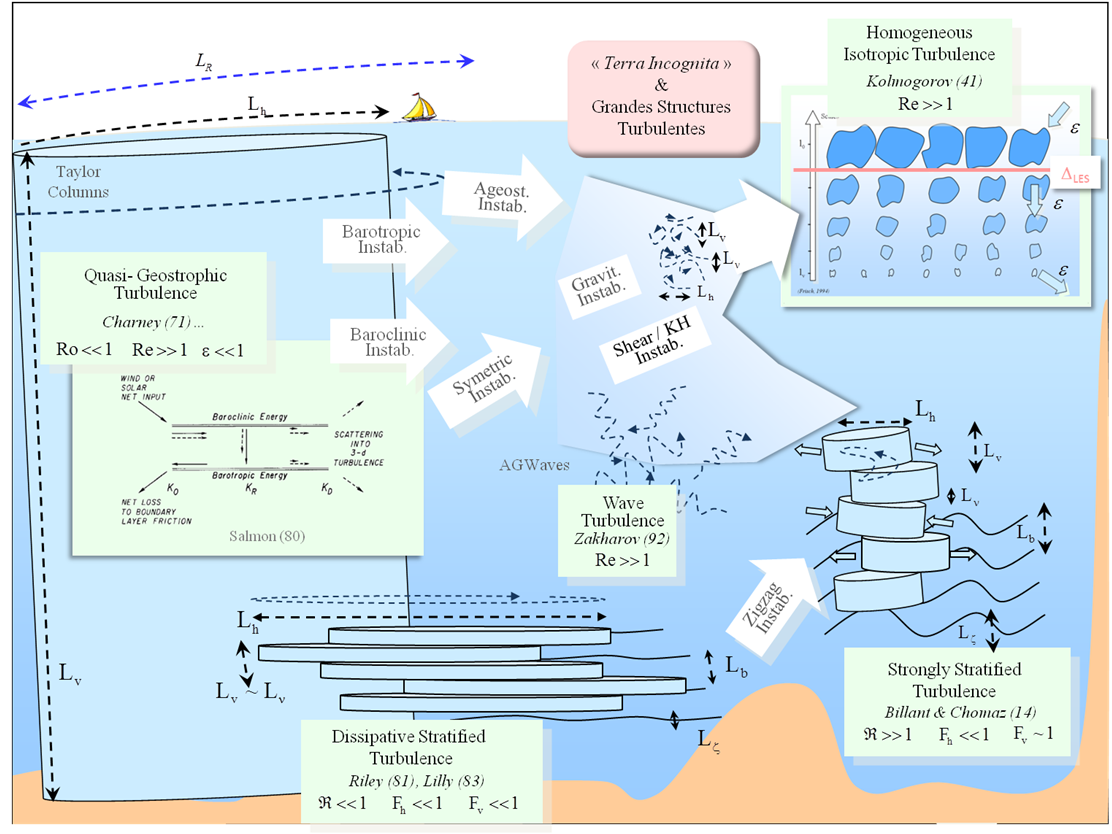
\includegraphics[width=0.8\textwidth]{./INTRO/Ocean_scales.png}
  \caption{\color{red}l'océan vu à travers ses cascades d'échelles, ses instabilités et ses principaux modèles de turbulence.\color{black}}
  \label{fig_ocean_scales}
\end{figure}
%\color{blue}
L'océan est soumis à/ mis en mouvements sous l'action de nombreux forçages par la pression atmosphérique, les marées astronomiques ou les flux de quantité de mouvement induits par le vent mais aussi par les flux de chaleur radiatifs ou par les flux de chaleur latente ou encore par les précipitations, les fleuves ou encore par évaporation... Ainsi présenté, l'océan peut donc être présenté comme un \textit{système dynamiquement ouvert}, l'ensemble des forçages auxquels il est soumis induisant un large spectre de processus dynamiques: houle, courants d'Ekman, upwelling ou downwelling, ondes de marée, marées internes, convection profonde, courants de gravité, panaches fluviaux... 


La dynamique de l'océan est variée, composée de processus dynamiques couvrant une large gamme autant spatiale que temporelle. La houle, les courants d'Ekman, les systèmes d'upwelling ou de downwelling, les ondes de marée, les marées internes, la convection profonde, les courants de gravité, ou encore les panaches fluviaux, 

, composée d'une large gamme de processus aux extensions géographiques 


%d'un large spectre de processus, on peut citer la houle, les courants d'Ekman, les systèmes d'upwelling ou de downwelling, les ondes de marée, les marées internes, la convection profonde, les courants de gravité, ou encore les panaches fluviaux... 

L'océan ne se résume toutefois pas à une somme de processus "forcés" dont la combinaison linéaire suffirait à expliquer sa dynamique propre. Ces processus interagissent en effet entre eux induisant d'importants \textit {mécanismes de transferts} entre les différentes gammes d'échelles spatiales et temporelles. Lorsque ces transferts prennent une forme cohérente dans quelques régions spécifiques du spectre, on parle de \textit{cascades d'échelles}. Les mécanismes débouchant sur ces transferts sont quant-à eux généralement associés à des \textit{instabilités dynamiques}.\\
\cite{salmon_baroclinic_1980} montrent par exemple qu'à méso-echelle\footnote{Région du spectre constitué d'échelles plus grande que le premier rayon de Rossby.} ces transferts s'organisent de façon cohérente sous la forme d'une \textit{cascade inverse} associée à des transferts énergétiques barotropes dirigés majoritairement vers les plus grandes échelles\footnote{Une telle cascade "inverse" est caractéristique de régimes de turbulence 2D.} alors que les transferts d'enstrophie\footnote{A l'image de l'énergie cinéatique cinétique pour la vitesse, l'enstrophie est définie comme la moitié du carré de la vorticité relative, i.e. du rotationnel de la vitesse.} sont quant à eux majoritairement dirigés vers les plus fines échelles. 
Les vents et les flux de chaleur induisent ainsi des structures dynamiques (baroclines) qui sont brisées lorsque l'écoulement devient instable \citep{vallis_atmospheric_2006}.
Les \textit{instabilités barotropes et baroclines} sont par conséquent au coeur de cette cascade dite inverse, elles rythment les transferts autour des rayons de Rossby\footnote{Échelle caractéristique de longueur caractérisant localement l'impact de la rotation du globe terrestre sur une colonne océanique de stratification donnée.} barotropes et baroclines dans les écoulements de mésoéchelles. On parle de régime de \textit{turbulence géostrophique} \citep{charney_geostrophic_1971} dans une région du spectre où stratification de la colonne d'eau et rotation du globe terrestre jouent \textit{in fine} des rôles prépondérants et sont associés à des équations de bilan équilibrées de quantité de mouvement. La cascade inverse demeure toutefois un modèle qualitatif fournissant une grille de lecture pour processus complexes et "non localisés" du le spectre océanique.\\
Des structures de sous-mésoéchelle reçoivent ainsi énergie et enstrophie et sont elles-aussi sujettes à un large éventail d'instabilités \citep{mcwilliams_submesoscale_2016}: instabilité agéostophique, symétrique, frontale, convective ou encore instabilités de cisaillement, instabilités baroclines dans la couche de mélange océanique, instabilités paramétriques des ondes internes... Dans cette région du spectre, l'impact de la rotation du globe terrestre est plus faible qu'à mésoéchelle mais la stratification contraint fortement la dynamique océanique débouchant sur des formes de turbulence dites "stratifiées": \textit{turbulence stratifiée dissipative}, \textit{turbulence fortement stratifiée}. l'instabilité "zig-zag" fait office de pont entre ces deux formes de turbulence).\\
Les myriades d'ondes de gravité internes et d'ondes de gravité de surface interagissent aussi au point de donner lieu à une forme particulière de turbulence: \textit{la turbulence d'onde}. Leur déferlement, leurs instabilités donnent généralement naissance à des "patchs turbulents" annoncés par l'apparition de grandes structures turbulentes.\\
En deçà de cette mésoéchelle (on parle de sous-mésoéchelle), prend naissance une autre cascade présentant une certaine cohérence, la \textit{cascade directe} ou cascade de Richardson au sein de laquelle l'énergie est transférée "directement" vers l'échelle de Kolmogorov au delà de laquelle la dissipation moléculaire est active. Si les théories décrivant les transferts à mésoéchelles ne permettent pas de routes directes vers la dissipation, les transferts de sous-mésoéchelle le permettent.
Les \textit{grandes structures turbulentes} marquent l'entrée de cette cascade directe, elles sont associées à des instabilités de cisaillement telles que les instabilités de Kelvin-Helmholtz. A \textit{micro-échelle}, le modèle de turbulence homogène et isotrope 3D décrit de façon simple cette cascade. Les échelles spatiales et temporelles des grandes structures turbulentes ne sont toutefois pas clairement définies: elles peuvent atteindre quelques dizaines de mètres au sein de la colonne d'eau mais peuvent aussi ne pas dépasser le mètre dans les couches de surface ou de fond.\\
Cascades d'échelles et modèles de turbulence décrivent ainsi des régions spécifiques du spectre spatio-temporel de l'océan qui présentent une certaine cohérence. Les divers types d'instabilités tissent quant-à elles des ponts entre ces régions. En toute rigueur, comprendre, expliquer, simuler (explicitement) ou modéliser (implicitement) le mélange turbulent, impliquent donc évidemment de représenter correctement l'ensemble du spectre océanique, ses transferts, ses cascades... Elle requière toutefois plus spécifiquement de reproduire précisément la cascade turbulente directe, i.e. le transfert "inertiel" d'énergie aboutissant à la région "dissipative" du spectre. Le point de départ de cette cascade n'est cependant pas clairement défini et varie aussi bien dans le temps que dans l'espace. Seule l'apparition souvent intermittente de grandes structures turbulentes permet de localiser spatialement et temporellement ce point de départ.\\
%Les grandes structures turbulentes marquent donc l'entrée de la cascade directe menant à la dissipation moléculaire. Elles sont ainsi à l'origine d'une cascade débouchant sur une réorganisation irréversible, diabatique de la colonne d'eau et d'un redistribution des "traceurs" passifs ou actifs. Parmi ces "traceurs", la masse volumique joue un rôle particulier dans la dynamique océanique: les masses d'eau sont par exemple "transportées" le long des surfaces isopycnales et le contenu en vorticité potentielle entre deux de ces surfaces isopycnales se conserve au cours du temps.\\
A. Scotti \citep{scotti_large_2010}, dans une revue sur la modélisation de l'océan, conclut qu’avec l'étude des grandes structures turbulentes, s'ouvrent les portes de la \textit{terra incognita}. Il reprend ainsi la conclusion de J.C. Wyngaard \citep{wyngaard_toward_2004} rédigée quelques années auparavant pour l'atmosphère. Cette terre inconnue, souvent aussi qualifiée de "zone grise" abritant les \textit{fines échelles océaniques}, est plus largement considérée comme la région particulièrement mal connue du spectre océanique dans laquelle la dynamique peut localement et temporairement basculer d'un équilibre simple entre un nombre limité de processus vers une dynamique non-linéaire complexe induisant une cascade d'instabilités dynamiques (directe) aboutissant à la dissipation moléculaire. 
\color{black}
%Cependant, l'océan (tout comme l'atmosphère) a un écoulement turbulent, c'est-à-dire chaotique et non-linéaire/ constitué d'une intéraction d'échelle.
%...
%Cette turbulence se manifeste en la décomposition des structures de grande échelles/synoptiques en des champs de plus petite structures/structures de plus en plus petites (transiant?) en intéractions les unes avec les autres (tourbillons, etc). Ainsi l'étude de l'océan peut se faire à bien des échelles spatiales et temporelles
%Ce manuscrit de thèse porte sur l'étude d'une dynamique dite de 'fine échelle', sur les processus / phénomènes océaniques . Il s'agira 
\color{blue}
\subsection{Rétroactions}
\label{subsection_retroactions}
Le mélange peut ainsi être présenté comme l'aboutissement de transferts et de cascades plus ou moins cohérentes mais quoiqu'il en soit très hétérogènes et intermittentes. Il ne constitue toutefois pas un puits sans fond ou un aller sans retour. Les flux diapycnaux modifient en effet les masses d'eau, la dissipation visqueuse qui "injecte" de la vorticité potentielle\footnote{La vorticité potentielle est une quantité, une substance d'après \cite{haynes_conservation_1990}, essentielle dans la description des écoulements stratifiés et en rotation qui est conservée par advection} près du fond... et constituent donc autant d'exemples de retroaction sur la grande échelle.\\
\cite{penney_2020} ont montré que le mélange était finalement capable de structurer les plus grandes échelles en mettant en évidence l'apparition à plus grande échelle de relations linéaires entre la masse volumique et les traceurs passifs qu'ils simulent.\\
La région du détroit de Gibraltar séparant la mer Méditerranée de l'océan Atlantique est à ce titre tout à fait exemplaire. Les masses d'eau méditerranéennes et atlantiques s'y croisent de façon tout aussi éphémère que brutale. Le mélange de ces deux masses d'eau induit par les fortes amplitudes de marée modifient in fine la salinité ou la quantité de mouvement de ces masses d'eau exerçant un contrôle sur la dynamique de l'ensemble du bassin Méditerranéen \citep{armi_1988}, scellant en quelques sortes le régime dynamique de l'ensemble du bassin et fixant vraisemblablement le contenu en vorticité potentielle du jet méditerranéen en Atlantique Nord.\\
La dissipation turbulente exerce donc une rétroaction sur les plus grandes échelles du spectre océanique: elle  structure les masses d'eau mais aussi la circulation océanique.
\color{black}
%(Revient plus en détail sur la turbulence, cas où mot est utilisé (turbulence géostrophique? vs cascade turbulente))
%Turbulence de mésoéchelle (instabilité barocline), ici on s'intéresse au début de la cascade turbulente directe définie par Kolmogorov. Les 2 sont similaires en ce qu'elles concernent le transfert d'énergie vers de plus fines échelles. Pour le cas de la turbulence de fine échelle, // mais va aussi aboutir à structuration de l'écoulement en lui-même. (La conservation de la vorticité potentielle (PV) peut agir comme un effet structurant de jet/courants...//méandres d'un jet / courant structurés par la conservation de la vorticité potentielle... PV générée par diabatic processes (in boundary layers?)...

%Cascade inverse???

\subsection{Le détroit de Gibraltar}
%(intérêt de la zone en vu du blabla précédent)
\color{blue}
Les talus continentaux, dorsales océaniques, les monts sous-marins isolés et autres détroits sont autant d'accidents bathymétriques qui canalisent, perturbent, modifient la circulation générale des masses d'eau océaniques et plus généralement la dynamique de l'océan. Les accidents bathymétriques sont localement le siège de régimes de couches limites particuliers entraînant quasi-systématiquement l'apparition de structures turbulentes très localisées spatialement et ouvrant ainsi les portes de la "terra incognita".\\
Le détroit de Gibraltar déjà cité dans le paragraphe précédent (\S \noparref{subsection_retroactions}) comme exemple de région abritant des processus de fine échelle structurant la dynamique océanique de grande échelle, constitue l'archétype de l'accident topographique contraignant fortement la dynamique océanique. Il est en effet le lieu de passage obligé des échanges entre les bassins méditerranéens et atlantiques nord.\\
\color{red}
Je te laisse compléter avec une présentation de la dynamique de cette région : marée + circulation générale => ressaut + ISW +... fort mélange.\\
\color{blue}
La dissipation turbulente est répartie de façon très hétérogène dans la colonne d'eau océanique, souvent préférentiellement dans les couches de surface et de fond et généralement sous la forme d'évènements intermittents (on parle de bouffées turbulentes). Ces caractéristiques compliquent grandement sa localisation et sa quantification même si son impact sur la circulation générale est maintenant reconnu et décrit de façon très qualitative \cite{de_lavergne_abyssal_2017}. La région du détroit de Gibraltar offre donc un terrain d'étude particulièrement pertinent pour qui souhaite étudier cette dissipation turbulente et ses rétroactions puisque les bouffées turbulentes semblent devoir être associées aux régimes dynamiques présentant de fortes amplitudes de marée (donc facilement localisables dans le temps) et au dessus des principaux seuils parsemant le détroit (donc facilement localisables géographiquement cette fois).\\
Le choix du détroit de Gibraltar comme région d'étude privilégiée pour mes travaux de doctorat se justifie donc à plusieurs titres. Elle est particulièrement adaptée pour une première exploration en \textit{terra incognita} puisque quelques portes ouvrant une voie vers cette terre inconnue semblent y être facilement localisables: les grandes structures turbulents peuvent être un peu plus facilement localisables, observables et donc simulées explicitement de façon numérique. Le détroit de Gibraltar est de plus une région de choix pour mieux appréhender l'impact (la rétroaction) que pourrait avoir la dissipation turbulente sur la circulation générale dans les bassins méditerranéens et nord-atlantiques: il s'agit donc d'une région de choix pour étudier comment cette dissipation peut structurer une dynamique à beaucoup plus grande échelle.
\color{black}

\color{blue}
\section{Une exploration des fines échelles océaniques}
%\color{red}
%(verrous puis objectif)
\subsection{Définir cette région du spectre océanique}
Objet central de mes travaux de doctorat, les \textit{fines échelles} océaniques doivent en premier lieu être clairement définies. Jusqu'ici, ces fines échelles ont plus spécifiquement été associées dans notre introduction (\S \noparref{subsection_intro1}) à la région du spectre océanique identifiée comme \textit{Terra incognita}.\\
Les fines échelles sont donc par la suite définies comme les échelles spatiales et temporelles de l'ensemble des processus et autres mécanismes dynamiques de \textit{sous-mésoéchelle} \citep{mcwilliams_submesoscale_2016} auxquels s'ajoutent les grandes structures turbulentes ouvrant la voie à la cascade directe et marquant l'entrée de la \textit{micro-échelle}.
 \color{black}

\subsection{Se donner les outils et les moyens d'une telle exploration}
\color{blue}
Toute entrée dans un territoire inconnu tel que la \textit{terra incognita} est associée à la reconnaissance et à la levée d'un certain nombre de difficultés. Dans le cas présent, ces "difficultés" prennent la forme de véritables \textit{verrous} d'ordres dynamiques et numériques.
\subsubsection{Verrous dynamiques.}
Un certain nombre de "verrous" dynamiques peuvent être identifiés. Les grandes structures turbulentes dont il est en particulier question ici sont le résultat de diverses instabilités "primaires" peuplant la méso et la sous-méso-échelle océaniques: instabilités barotrope, barocline, symétrique, zig-zag, agéostrophique, paramétrique des ondes internes, etc... Ces mécanismes de déstabilisation peuvent être vus comme brisant des structures, des processus, des équilibres subtils régissant localement et de façon éphémère et intermittente la dynamique de l'océan. Leur exploration relève par conséquent plus d'une approche stochastique que purement déterministe.\\
Les grandes structures turbulentes constituent de plus des processus certes importants mais néanmoins indissociables des transferts d'échelles auxquels elles sont associées. Leur étude requiert donc la prise en compte simultanée de régions étendues du spectre océanique.\\
Ni les échelles spatiales ni les échelles temporelles des instabilités de cisaillement ne sont clairement identifiables à partir de grandeurs caractéristiques comme le peuvent être les rayons de Rossby pour la méso-échelle et les instabilités barotropes et baroclines.
\subsubsection{Verrous numériques.}
Les grandes structures turbulentes étaient traditionnellement l'apanage des modèles "sous-maille" dans les configurations océaniques côtières, régionales et à fortiori globales. N'étant par conséquent pas universels, ces modèles "sous-maille" rendent la simulation très dépendante du lieu et de la période étudiés: les "modèles de fermeture" doivent en effet être ajustés et confrontés à la réalité avec comme principal enjeu le choix du modèle et la détermination des paramètres physiques ou numériques qu’il inclut nécessairement. Si la réalisation de LES est envisageable et envisagées dans l’océan intérieur et peut donc être appuyée sur des modèles de turbulence plus universels et plus simple, elle demeure par contre hors d’atteinte dans les couches limites de surface et fond, régions dans lesquelles leurs échelles spatiales caractéristiques peuvent considérablement décroître pour être finalement de l'ordre du mètre. Des approches dites "zonales" doivent par conséquent être envisagées.
La simulation explicite des grandes structures turbulents engendre l'utilisation de grilles de calcul à très haute résolution sur des régions océaniques à priori relativement étendues. Elle requière donc un nouvel effort de réduction du coût de calcul. CROCO est en effet conçu et développé pour être un code efficace mais ce qu'il est aujourd'hui possible de simuler explicitement dans un détroit d'extension réduite doit être généralisé à des sous-bassins et à des plateaux continentaux de plus grande extension avec, très vraisemblablement, une résolution raffinée. Nous avons mené à bien une première étude de faisabilité au sein de notre petit groupe CROCO / LA débouchant sur le portage du code sur GPU sur des machines hétérogènes CPU / GPU. Le nécessaire travail d’optimisation des performances est désormais en conduit en très étroite collaboration avec les équipes INRIA. Le surcoût de calcul associé à la compressibilité et à la remise en cause de l'hypothèse hydrostatique a par exemple dors et déjà pu être effacé en déportant sur GPU l'intégration du mode rapide compressible.


\color{black}
\subsection{Simuler explicitement les fines échelles}
\color{blue}
Explorer numériquement les fines échelles océaniques implique de simuler explicitement les grandes structures turbulentes et l'on entre ainsi de plain-pied dans une approche numérique dite \textit{LES (pour \textit{Large Eddy Simulation})}.\\
La promesse d’une puissance de calcul pétaflopique puis exaflopique a, en théorie au moins, ouvert les portes de la simulation des grandes structures turbulentes (LES) pour l’océan et l’atmosphère. Les météorologues ont par exemple rapidement su tirer parti des moyens de calcul disponibles : des algorithmes dédiés ont vu le jour dès le début des années 2000 débouchant sur des codes numériques tels que WRF en version compressible ou Méso-NH en version anélastique. Ces deux types de codes permettent, chacun avec leurs spécificités, d’aborder la simulation de la cascade turbulente directe en représentant explicitement les plus grandes structures turbulentes dans l’atmosphère.
Les modèles océaniques n’ont pas été immédiatement en mesure de franchir ce cap de la LES en grande partie à cause de la présence d’une surface libre aux conséquences dynamiques multiples. La surface libre rend en particulier plus complexe la relaxation de l’hypothèse hydrostatique. Dans la foulée de l’ANR COMMODO rassemblant au milieu des années 2010 l’ensemble des équipes françaises travaillant sur la modélisation de l’océan, les équipes de recherche en océanographie dynamique et en mathématiques partenaires du projet CROCO se sont associées pour développer une nouvelle génération de codes capables d'explorer la "Terra Incognita". Un Groupement de Recherche éponyme est né associant l’université de Toulouse et les principaux organismes de recherche en informatique et en océanographie français: l’IRD, INRIA, le CNRS-INSU, l’IFREMER et le SHOM. En 2021, l’IRD a entériné la constitution d’un GdRi CROCO tourné vers nos partenaires au Sud.\\
Plusieurs pré-requis ont toutefois dû être satisfaits avant de lancer une exploration numérique des grandes structures turbulentes dans un contexte réaliste aussi complexe que celui du détroit de Gibraltar.
L'hypothèse hydrostatique, elle-aussi héritée du code ROMS, devait à minima être remise en cause en demeurant dans le contexte d'un océan à surface libre. Ceci fut chose en fait en relaxant aussi l'hypothèse de Boussinesq comme préconisée dans un contexte océanique par \cite{auclair_non-hydrostatic_2018}. L'héritage reçu du code américain ROMS \citep{shchepetkin_regional_2005} avait fait de CROCO un code particulièrement efficace dont le coeur numérique (son time-splitting, ses schémas numériques...) a été spécifiquement conçu pour limiter les coûts de calcul et l'utilisation de l'espace mémoire. Ce niveau de performance numérique a été maintenu pour son noyau numérique compressible et non-hydrostatique dans un contexte massivement parallèle.\\
De nouvelles recherches ont été entamées en parallèle de mes travaux de thèse pour d'une part porté sur le code sur une nouvelle génération de processeurs dits hétérogènes (associant CPU et GPU) et d'autre part permettre le raffinement local de la dynamique océanique par imbrication de configurations LES dans des maquettes numériques régionales très étendues. Les maquettes que j'ai développées ou co-développées dans le cadre de mes travaux de thèse ont servi de configuration-tests pour l'ensemble de ces développements transformant le détroit de Gibraltar en une région de démonstration.\\
\color{blue}
\subsection{Où l'on justifie une démarche scientifique pour cette exploration...}
\color{black}
Les années de thèse ont eu pour objectif de mettre en place outil sur une région particulièrement/// Simuler explicitement, observer, quantifier, pour explorer intéraction d'echelles sur spectre élargi


\section{Plan du manuscrit}




%Morceaux de intro GBR3D : 
%The amplitude of the exchange varies over timescales larger than the semi-diurnal tide. The lower frequencies (whether seasonal or inter-annual) are usually linked to atmospheric forcing over the Mediterranean \citep{sanchez-roman_2012}. The tidal eddy-fluxes have their own variability associated to the spring-tide cycle and to the monthly tides, with for example a greater depth and stronger shear during neap tides, but more intense mixing during spring tide \citep{naranjo_2014,vargas_2006}.\color{red}(enlever? sert à rien? que dans intro plus générale???)\color{black}


%Numerical models are discretized and have a treshold resolution under which phyisical pehomenons cannot be represented explicitely. Particularly, diffusion and ... processes,  among other parametrisations of processes like surface exchanges, radiation that occur at molecular or submolecular scales. Diffusion and dissipation are molecular in nature as a , energy flux, but more broadly speaking, dissipation is the transfer of energy from great scales to small scales. In a stratified fluid, this dissipation is accompagnied by mixing , ie a lewoering of potential energy, or more accurately and explained i paragraph ..., of the background potential energy.
%Broadly for oceanic (or more generally geophyisic?) models classification on DNS, LES, and RANS. DNS has molecular dissipation
%For the discussions simply coining as LES is not sufficient but need to precise LES in regard to which phenomenon. For exemplein chapoter ... of this manuscript, coined LES because primary instabilities of the flow. However, the primary instabilities that are known to exist at upper and lower boundaries of teh water column are not represented and are parametrized, so in regard to the dissipation those process not LES. 
%To this considerations, one must also not forget that the discretisation itself introduces numerical dissipation unless using centered schemes (computationnally impossible).



%\subparagraph{Conclusion générale/dans le manuscrit}
%Les simulations ... sont première LES maisblablablablabla (trad ce que avait dit...). Besoin outil diagnostique du mélange, chapitre prochain...





%%%%%%%%%%%%%%%%%%%%%%%%%%%%%%%%%%%%%%%%%%%%%%%%%%%%%%%%%%


\chapter{Mod\'elisation  Repr\'esentation de l'oc\'ean et de son m\'elange}
\begin{itemize}
\item conservation masses/qdm, discretisation numérique, échelles (RANS/LES(/DNS)), paramétrisation du mélange, fermeture turb (Smago/GLS...)
\item contenu en PV
\item definition BPE, eq d'évolution 'générale'
\item code CROCO (ou code CROCO en premisce de chap 3 GBR2D????(sinon parait cours?)GBR2D parle passage hydro a NBQ...)
\end{itemize}



\section{Résumé du chapitre en français}
Le présent chapitre présente de façon détaillée le \textit{modèle d'océan} utilisé dans le cadre de ma thèse pour simuler numériquement les grandes échelles turbulentes (ou LES$^{\noparref{LES}}$) dans la région du détroit de Gibraltar mais aussi, plus généralement, pour développer des modèles analytiques simplifiés de processus au service de cette approche numérique. Plusieurs sections du chapitre ont été intégrées à des publications acceptées \citep{hilt_2020}, \citep{auclair_modied_2021} ou en cours de rédaction  \citep{auclair_NBQ1_2021} mais aussi au rapport d'études du programme amont PROTEVS Gibraltar du SHOM \citep{auclair_modelisation_2019}. L'ensemble du chapitre est par conséquent rédigé en anglais.

Dans une première partie (\S \ref{section_prim_eq}) sont introduites les équations de conservations usuelles de l'océanographie physique, dont les équations de Navier-Stokes, point de départ du développement du \textit{modèle d'océan}. Le choix est ensuite fait de se placer dans le contexte d'une grille verticale curviligne qui permet d'épouser la forme des fonds marins et de suivre les mouvements de la surface libre de l'océan (dont un certain nombres de développements ont aussi présentés en annexe (\noparref{section_annexe2})). 
%Dans ce cadre, l'expression de l'évolution de l'énergie potentielle gravitationnelle (PE) et de ses sous-compartiments, énergie potentielle disponible (APE) et énergie potentielle de "background" (BPE), est développée dans un volume local d'océan (section \ref{section_PE_chap2}). En particulier, l'évolution de la BPE fait apparaître un terme source lié aux mouvements de la surface libre. Comme l'évolution de la BPE est lié au mélange diapycnale, la bonne expression de son bilan est impérative afin de faire des diagnostics de quantifications de mélange se basant sur cette méthode. %FA%

Dans la deuxième partie du chapitre (section \ref{section_croco}), est présenté le fonctionnement du code communautaire à cœur non-hydrostatique, compressible et à surface libre CROCO, basé sur le \textit{modèle d'océan} de la première partie. 
L'implémentation numérique de ce \textit{modèle d'océan} a demandé d'importants développements tant algorithmiques que numériques, développements qui ne peuvent être menés à bien s'ils miment directement la physique de l'océan. Parce qu'il est très général, ce \textit{modèle d'océan} peut réaliser la synthèse de processus dynamiques dans une gamme très étendue d'échelles spatio-temporelles depuis la circulation basse fréquence, jusqu'aux ondes acoustiques. Ce sont plus spécifiquement les plus fines échelles et les plus hautes fréquences qui peuvent imposer les plus fortes restrictions à l'approche numérique envisagée ; ce sont donc les processus associés et en particulier les processus ondulatoires acoustiques ou gravitaires qui ont été étudiés en priorité. 

%Ce \textit{modèle d'océan} est suffisamment général pour autoriser la représentation explicite d'une large gamme de processus allant des ondes et modes acoustiques dans un océan compressible aux structures turbulentes fondamentalement non-hydrostatiques de \textit{fine échelle} (associées par exemple à des instabilités de Kelvin-Helmholtz) en passant par des processus ondulatoires internes de grande amplitude (tels que les solitons).

J'ai participé à une partie des développements de CROCO durant ma thèse, sur le plan purement numérique tout d'abord, avec l'implémentation et l'évaluation de nouveaux schémas numériques dans un contexte pleinement réaliste et la mise en œuvre de stratégies originales pour la LES. Sur le plan de la dynamique océanique ensuite, avec la réalisation d'études de processus de fines échelles et l'étude des interactions complexes entre ces processus.

%Ce \textit{modèle d'océan} a de plus servi de base au développement dans le cadre de ma thèse de diagnostiques originaux dédiés à la simulation des grandes échelles turbulentes océaniques (LES) dans un contexte réaliste: évaluation quantitative du mélange turbulent (\S \noparref{chapter_bpe}), mise en évidence et caractérisation de ces structures, études de ressauts hydrauliques (\S \noparref{PartDiag3D})...

En parallèle des développements numériques et des travaux sur la dynamique de la région du détroit de Gibraltar menés dans le cadre de la présente thèse de doctorat, a été développé et publié un modèle analytique suffisamment général pour décrire la dispersion des ondes et des modes acoustiques, des ondes et des modes internes de gravité ou encore des ondes de gravité de surface \citep{auclair_modied_2021}. Le modèle analytique de dispersion a de plus été utilisé pour explorer la dynamique ondulatoire dans la région du détroit de Gibraltar.
J'ai participé et co-signé cette étude en support du développement numérique de CROCO, étude qui n'a pas été incluse dans le présent manuscrit.

Dans ce qui suit du présent chapitre, c'est l'anglais qui est utilisé pour les raisons évoquées précédemment.

%Dans une première partie, les équations analytiques servant de base à ce \textit{modèle d'océan} sont présentées (\noparref{section_prim_eq}), l'approche numérique choisie et co-développée pour le coeur numérique non-hydrostatique, compressible et à surface libre de CROCO est détaillée en partie \ref{section_croco}. Un certain nombre de développements sont enfin présentés dans les annexes (\noparref{section_annexe2}).


\section{A non-hydrostatic, compressible, free-surface ocean model}
\label{section_prim_eq}

%%%%%%%%%%%%%%%%%%%%%%%%%%%%%%%%%%%%%%%%%%%%%%%%%%%%%%%%%%%%%%%%%%%%%%%%%%%%%
 %----------------------------------------------------------------------------
 \subsection{Continuous free-surface compressible equations in z-coordinates}
 %----------------------------------------------------------------------------
\label{subsectiongenesystem}
\subsubsection{Model equations in conservative form}
Conservation of mass, conservation of momentum (Newton's second law of motion), conservation of total energy (first law of thermodynamics) and conservation of any tracers are the backbones of ocean dynamics. In the ocean, the conservation of mass can be written as a prognostic equation for density (written $\rho$), the conservation of momentum leads to prognostic equations for the three components of momentum (written $\rho \mathbf{v}$) and the conservation of total energy (or first law of thermodynamics) can be stated as a prognostic equation for potential temperature ($\theta$). The conservation of chemical species can then be expressed as a prognostic equation for salinity ($S$). These conservation equations consequently lead to the following general system of prognostic equations (expressed in flux form):
\begin{subequations}
 \begin{alignat}{2}
 \displaystyle
 \label{NS_a} 
 & \frac{\partial\rho}{\partial t} &&= - \mathbf{\nabla}\cdot(\rho \mathbf{v})\\[3mm]  
 \label{NS_b}
 & \frac{\partial \rho \mathbf{v}}{\partial t} 
	 &&= -\mathbf{\nabla}\cdot(\rho \mathbf{v}\otimes \mathbf{v}) 
	  \color{black} -2\rho\ \mathbf{\Omega}\ \times \ \mathbf{v} \color{black} -\mathbf{\nabla}p + 		
	\mathbf{\nabla}\cdot\left(
	\mu(\mathbf{\nabla}\mathbf{v}+\mathbf{\nabla}\mathbf{v}^{\ T})
 +\mu_2(\mathbf{\nabla}\cdot\mathbf{v})\ \mathbf{I}\ \right)
 +\rho \mathbf{g}\\
 %
 \label{NS_c}
 & \frac{\partial \rho \theta}{\partial t} &&=-\mathbf{\nabla}\cdot(\rho \theta\mathbf{v})
 +\mathbf{\nabla}\cdot\color{black}(\kappa_\theta\mathbf{\nabla}{\theta})\color{black}\\[3mm]
 %
 \label{NS_d}
 & \frac{\partial \rho S}{\partial t} &&=-\mathbf{\nabla}\cdot(\rho S\mathbf{v})
 +\mathbf{\nabla}\cdot\color{black}(\kappa_S\mathbf{\nabla}{S})\color{black}
 %
  \end{alignat}
\end{subequations}
with $\mu$, $\mu_2$, $\kappa_T$ and $\kappa_S$ respectively the dynamical and bulk viscosities and the thermal and salt diffusivities. $\mathbf{\Omega}$ is the earth instant rotation vector.
Assuming that variables are in thermodynamic equilibrium, the equation of state (EOS) can be formulated as a non-linear, diagnostic functional relation between temperature, salinity, density and (total) pressure (written $p$):
\begin{equation}
 \label{NS_e}
 \rho = \rho_{eos}[\theta,S,p]
\end{equation}

\subsubsection{Boundary conditions}
The position of the interface separating the ocean and the atmosphere must additionally be calculated and is introduced as a boundary condition. This can be achieved by stating that a salty-water particles that is just bellow this interface in the ocean, remains at the interface, leading to the surface kinematic relation:
\begin{equation}
  \displaystyle
  \label{NS_BC2}
  %\frac{\textrm{d}\zeta(\mathbf{x}_{\scriptscriptstyle H},t)}{\textrm{dt}}=w(\mathbf{x}_{\scriptscriptstyle H},z=\zeta)
  \frac{\partial \zeta}{\partial t}=w(\mathbf{x}_{\scriptscriptstyle H},z=\zeta)-\mathbf{v}_H(\mathbf{x}_{\scriptscriptstyle H},z=\zeta)\cdot\mathbf{\nabla}_H\zeta
\end{equation}
where $\zeta$ is the free-surface anomaly in the vicinity of the geoid and subscribe $H$ indicates that only the horizontal component is considered. Assuming then that ocean water cannot penetrate the ocean bottom (at depth $z=-H$):
\begin{equation}
 \displaystyle
 \label{NS_BC0}
  \mathbf{v}(\mathbf{x}_{\scriptscriptstyle H},z=-H)=\mathbf{0}
\end{equation}
Neglecting surface-tension pressure drop, the boundary condition for pressure at the surface of the ocean is given by:
\begin{equation}
 \displaystyle
 \label{NS_BC1}
  p(\mathbf{x}_{\scriptscriptstyle H},z=\zeta,t)= p_{atm}
\end{equation}
with $p_{atm}$ the atmospheric pressure above the surface of the ocean.
The resulting system of prognostic equations, diagnostic relations and boundary conditions leads to a non-linear problem whose main characteristics is the wild spectrum of dynamic processes involved (see for instance \cite{gill_atmosphere-ocean_1982} or \cite{vallis_atmospheric_2006}). Periodic processes such as ocean waves can give a comprehensive overview of the extension of space-time spectrum of transient processes which can propagate in the ocean and \cite{auclair_modied_2021} derive a compressible, free-surface, stratified model of two dispersion relations for wave-numbers and pulsation gathering acoustic, surface and internal waves and insisting on the modification of the dispersion of gravity (acoustic) waves by compressibility (gravity and stratification).

Formulated thus, the system of Navier-Stokes and conservation equations for a free-surface ocean can, at least in theory, be integrated straightforwardly. All variables but the pressure have their own prognostic equation and pressure can be diagnosed from the EOS \ref{NS_e}. Note that the system can be reformulated so that pressure is also given by a prognostic equation.

\subsubsection{Evolution of the density field}
For a linear approximation of the equation of state, a simple evolution equation of $\rho$ can be obtained as a combination of equations \ref{NS_c} and \ref{NS_d} leading to:
\begin{equation}
\displaystyle
\frac{d \rho}{d t}=
%\frac{\partial}{\partial x} \bigg(\kappa_\rho^h \frac{\partial \rho}{\partial x}\bigg\rvert_{tz}\bigg)_{tz}
%+ \frac{\partial}{\partial z} \bigg( \kappa \frac{\partial \rho}{\partial z}\bigg\rvert_{tx}\bigg)_{tx} 
 \mathbf{\nabla}\cdot\color{black}(\kappa_{\rho} \mathbf{\nabla}{\rho})
\label{eq_diff_cart}
\end{equation}
where $\kappa_{\rho}$ is the equivalent diffusivity of density.

 %----------------------------------------------------------------------------  
 %\subsection{Density and pressure decomposition}
 %----------------------------------------------------------------------------
 
\subsection{Terrain-following coordinates}
\label{subsection_scoord}

 %%%%%%%%%%%%%%%%%%%%%%%%%%%%%%%%%%%%%%%%%%%%%%%%%%%%%%%%%%%%%%%%%%%%%%%%%%%%%
\subsubsection{Definition}
%%%%%%%%%%%%%%%%%%%%%%%%%%%%%%%%%%%%%%%%%%%%%%%%%%%%%%%%%%%%%%%%%%%%%%%%%%%%%
The capacity of numerical models to mimic the evolution of global or regional oceanic circulation relies on horizontal and vertical definition of the grid on which the Navier-Stokes and conservation equations previously defined are solved and integrated in time.

Due to considerations of the representation of bathymetric features and free-surface evolutions, terrain-following coordinates, or S-coordinates, are chosen for the vertical discretisation. They are generally defined on generalized constant-$s$ surfaces with $s$ given by:
\begin{equation}
 \displaystyle
 s=s(x,y,z,t)=s(\mathbf{x},t)
\end{equation}
requiring thus that $s$ be a monotonic function of the vertical coordinate $z$:
\begin{equation}
 \displaystyle
 \frac{\partial s}{\partial z}\bigg\vert_{xyt}\ne 0
\end{equation}
$\partial s / \partial z$ is continuous and single-signed (either strictly positive or negative).

%%%%%%%%%%%%%%%%%%%%%%%%%%%%%%%%%%%%%%%%%%%%%%%%%%%%%%%%%%%%%%%%%%%%%%%%%%%%%
\subsubsection{Examples}
%%%%%%%%%%%%%%%%%%%%%%%%%%%%%%%%%%%%%%%%%%%%%%%%%%%%%%%%%%%%%%%%%%%%%%%%%%%%%
Several examples and comparisons on the choice of $s(\mathbf{x},t)$ are given in chapter 6 of \citet{griffies_fundamentals_2004}.
Following  \citet{shchepetkin_regional_2005},  less general $\sigma$-coordinates can be defined by:
\begin{equation}
 \displaystyle
 z(\mathbf{x},\sigma,t)=\sigma H(\mathbf{x_h})\quad or\quad z(\mathbf{x},\sigma,t)=\sigma(H(\mathbf{x_h})+\zeta(\mathbf{x_h},t))+\zeta(\mathbf{x_h},t)
\end{equation}
%or:
%\begin{equation}
% \displaystyle
% z(\mathbf{x},\sigma,t)=\sigma(H+\zeta)+\zeta
%\end{equation}
where $H(\mathbf{x_h})=H(\mathbf{x,y})$ is the bottom topography and $\zeta(\mathbf{x_h},t)$ the surface elevation anomaly. Its generalization to s-coordinates is defined by:
\begin{equation}
 \displaystyle
 z(\mathbf{x},s,t)=\mathcal{S}(s) H(\mathbf{x_h})
\end{equation}
which is currently written:
\begin{equation}
 \displaystyle
 z(\mathbf{x},\sigma,t)=\mathcal{S}(\sigma) H(\mathbf{x_h})
\end{equation}
and $S(\sigma)$ can be a non-linear function. Some current definitions are presented on the Wiki-Roms web-site \footnote{\url{https://www.myroms.org/wiki/Vertical_S-coordinate}}.


%%%%%%%%%%%%%%%%%%%%%%%%%%%%%%%%%%%%%%%%%%%%%%%%%%%%%%%%%%%%%%%%%%%%%%%%%%%%%
\subsubsection{Vertical velocities}
%%%%%%%%%%%%%%%%%%%%%%%%%%%%%%%%%%%%%%%%%%%%%%%%%%%%%%%%%%%%%%%%%%%%%%%%%%%%%
The definition of such a new vertical coordinate requires the derivation of the associated vertical velocity at the grid point. Using the coordinate transformation presented in section \ref{annexe_coordS} of appendix \ref{annexe_ocmod},  $w \equiv v_z$ can be decomposed as :
\begin{subequations}
  \begin{alignat}{2}
  \displaystyle 
	& v_z &&\equiv \frac{d z}{d t}\\
	& &&=\underbrace{\underbrace{\frac{\partial z}{\partial s}\bigg\rvert_{tx}}_{\equiv h} \frac{d s}{dt}}_{\equiv v_s}
	+\underbrace{\frac{\partial z}{\partial x}\bigg\rvert_{ts} \underbrace{\frac{d x}{dt}}_{\equiv u}
	+\frac{\partial z}{\partial t}\bigg\rvert_{xs} \underbrace{\frac{d t}{dt}}_{=1}}_{=\frac{dz}{dt}\big\rvert_{s}}\\[4mm]
	& &&=\frac{\partial z}{\partial s}\bigg\rvert_{tx} \frac{d s}{dt}
	+\frac{d z}{d t}\bigg\rvert_{s} \\[4mm]
	& &&=\ \ h \frac{d s}{dt}\quad
	+\frac{d z}{d t}\bigg\rvert_{s}\\[4mm]
	& &&=
	\ \ v_s 
	\qquad+\underbrace{\frac{\partial z}{\partial t}\bigg\rvert_{xs}
	+u \frac{\partial z}{\partial x}\bigg\rvert_{ts}}
	_{\frac{d z}{d t}\big\rvert_{s}=v_{\Sigma,z}}
  \end{alignat}
  \label{eq_vertvelcomp}
\end{subequations}
where:
\begin{equation}
	\displaystyle
	h\equiv\frac{\partial z}{\partial s}\bigg\rvert_{tx} \ \ \text{and} \ \
	v_s\equiv h\frac{d s}{d t}
\end{equation}

In other words, the vertical velocity is the composition of $v_{\Sigma,z}$ (the vertical component of the velocity of the constant-$s$ surface as it moves), and $v_s$ (the velocity through this same surface). An important aspect of this computation is that $v_s$ remains a velocity along the vertical axes since no change of direction of the axes is made.

%%%%%%%%%%%%%%%%%%%%%%%%%%%%%%%%%%%%%%%%%%%%%%%%%%%%%%%%%%%%%%%%%%%%%%%%%%%%%%
%\subsubsection{Vertical velocities in $"\sigma"$-coordinates}
%%%%%%%%%%%%%%%%%%%%%%%%%%%%%%%%%%%%%%%%%%%%%%%%%%%%%%%%%%%%%%%%%%%%%%%%%%%%%
In the more restrictive case where $\sigma$-coordinates are used:
% In $\sigma$-coordinates:
\begin{equation}
 \displaystyle
 \sigma=\frac{z-\zeta}{H+\zeta}
\end{equation}
and as a consequence:
\begin{equation}
 \displaystyle
 v_z=w=\mathbf{u}_z.\mathbf{v}
=\frac{dz}{dt}=\underbrace{(H+\zeta)\frac{d\sigma}{dt}}_{\equiv v_{\sigma}}
 +(\sigma-1)\frac{dH}{dt}
 +\sigma\frac{d\zeta}{dt}
\end{equation}
where in $\sigma$-coordinates:
\begin{equation}
 \displaystyle
v_{\sigma}=(H+\zeta)\frac{d\sigma}{dt}
\end{equation}

 \section{CROCO: a numerical implementation of the non-hydrostatic, compressible, free-surface \textit{ocean model}}
 \label{section_croco}
 
%----------------------------------------------------------------------------  
\subsection{Numerical implementation of the \textit{ocean model}}
%----------------------------------------------------------------------------
Ocean models whether dedicated to global, regional or even coastal scales are traditionally based on the Boussinesq, hydrostatic assumptions \citep{griffies_elements_2012,shchepetkin_regional_2005}. The present study is a step toward the explicit simulation of at least the largest turbulent eddies in a realistic context and, as a consequence, a non-hydrostatic numerical approach is required. \cite{Auclair2018} concluded that an efficient non-hydrostatic, free-surface, mode-splitting numerical model of the ocean could be designed relaxing also the Boussinesq approximation. Doing so, the authors chose to work with local equations and they do not solve for a 3D Poisson equation to diagnose total pressure. They consequently follow the choices made in meso-scale atmospheric modeling by \cite{skamarock_prototypes_2001}. The compressible (non-Boussinesq) approach is original in ocean modeling and in particular in free-surface, ocean modeling. Indeed \cite{marshall_finite-volume_1997} or \cite{auclair_non-hydrostatic_2011} chose to retain the Boussinesq assumption. A consequence of \cite{Auclair2018}'s choice is that the complete \textit{ocean model} presented in \S\ref{section_prim_eq} can be solved numerically.

The computing cost of such a non-hydrostatic, compressible, free-surface approach can quickly become prohibitive especially because the explicit modeling of fine scales requires high-resolution grids. Following the conclusions of the COMODO french community\footnote{COMODO gathered the french ocean modeling community. It was sponsored by the French ANR eponymous project (2011-2016).}, the compressible and free-surface algorithm developed by \cite{Auclair2018} has been implemented in the ROMS-AGRIF branch of the ROMS ocean models \citep{shchepetkin_regional_2005}. This choice was justified by the great efficiency of Shchepetkin's time-splitting and time-stepping and more generally by the experience accumulated in ROMS community during the last two decades.

The simulations of the strait of Gibraltar presented in chapters \ref{chapGBR2D} and \ref{chapGBR3D} were the very first realistic implementation of the non-hydrostatic, compressible, free-surface kernel of CROCO \citep{hilt_2020}.
\color{black}
%----------------------------------------------------------------------------  
\subsection{Time-splitting}
%----------------------------------------------------------------------------
\subsubsection{Dynamical time-scales}
Numerical constraints can conveniently be enumerated in terms of time-scales of dynamical "transfers" of tracer, pressure or velocity anomalies in the ocean. Advection, diffusion or radiation by gravity or acoustic waves are examples of such transfers. For a given length-scale (such as a model grid scale), maximum characteristic velocities can give  an order of magnitude for the most restrictive time-scales for each type of "transfer".\\
To derive the main characteristic length scales, the pressure and density anomalies are first conveniently defined with respect to the hydrostatic rest state leading to the pressure decomposition:
\begin{equation}
	\displaystyle
	\label{decompoP_0}
	p(\mathbf{x},t)=p_h(\mathbf{x},t)+\delta p(\mathbf{x},t)
\end{equation}
with $p_h(\mathbf{x},t)$ the hydrostatic pressure component and $\delta p(\mathbf{x},t)$ an anomaly. The former is defined by $\partial_z p_h=-\rho_h(\mathbf{x},t) g$ where $\rho_h(\mathbf{x},t)$ can be chosen as the slowly-varying, statically-stable field of density. Based on this pressure decomposition, a first-order Taylor expansion of the density field can be carried out :
\begin{equation}
  \displaystyle 
	\label{decompor_0}
  \rho(T,S,p)=\rho_{\theta S}(T,S,p_0)+\frac{p_h+\delta p-p_0}{c_s^2}+\mathcal{O}(\delta p^2)
\end{equation}
for a reference, slow component of pressure $p_0$ which is most often chosen different from the hydrostatic pressure in numerical models.
Numerical constraints relative to the various transfers of anomalies can basically be classified into three categories depending if they are associated to compressibility (acoustic waves..), surface-induced processes (surface gravity waves...) or internal-ocean (incompressible) processes (internal gravity waves, advection, diffusion, buoyancy-induced processes...). Orders of magnitude of maximum velocities in a deep ocean of each category are respectively given by $v[\delta p]\approx \mathcal{O}(1500\ m/s)$, $v[p_\zeta]\approx\sqrt{g H}\approx \mathcal{O}(100\ m/s)$ and $v[p_{int},\ ...]\approx \mathcal{O}(1\ m/s)$ leading to at least two spectral gaps in terms of velocities in the ocean:
\begin{equation}
	\displaystyle
	\label{velocityscales}
	v[p_{int},\ ...] \ll v[p_\zeta] \ll v[\delta p]
\end{equation} 
This hierarchy of velocity scales (and thus timescales for a fixed grid-scale) and the associated gaps constitute the basis to develop time-splitting approaches for numerical models of the ocean.
Under free-surface, Boussinesq and hydrostatic assumptions, the time-splitting procedure implemented in ROMS model \citep{shchepetkin_regional_2005} filters for instance acoustic and non-hydrostatic processes and takes advantage of the gap $v[p_{int},\ ...] \ll v[p_\zeta]$. It can be formulated as a decomposition of the pressure between a 2D surface-induced pressure-component (named external or barotropic-like component) $\bar{p}_h(\mathbf{x},t)$ and a 3D density-induced (internal or baroclinic-like) pressure-component $p_h'(\mathbf{x},t)$. 
The time-splitting approach for a more general free-surface, non-hydrostatic and compressible ocean can also be based on \ref{velocityscales}. The procedure is yet different from that used for hydrostatic ocean models. In the latter, coupling is based on the separation of the velocity field between a barotropic-like, depth-averaged component and a baroclinic-like anomaly. The faster, surface-induced component of the pressure force is integrated with a small time-step and after each integration sequence of the external mode, the depth-averaged component of the internal-mode velocity is forced to fit to the external-mode, depth-averaged velocity. Separating the "fast" and "slow" components of momentum in a compressible model to integrate them separately is not that simple and more importantly, it is not even necessary. The time-splitting procedure proposed in CROCO compressible kernel is indeed based on the splitting of the terms on the Right-Hand-Side (hereafter RHS) of the prognostic and diagnostic equations of the ocean model. Two coupled models (hereafter called the slow and fast numerical kernels) are then integrated in turn. The slow (respectively fast) kernel is advanced with a large (small) time-step computing explicitly slowly-varying (rapidly-varying) terms at the RHS and implicitly the remaining terms. A time-filtering procedure is additionally implemented to force both the slow and fast mode in a similar way as \citet{shchepetkin_regional_2005}.

\subsubsection{Pressure and density decomposition}
The splitting of the processes based on the magnitude of their time-scale relies essentially on a decomposition of the pressure and density fields. Following \cite{auclair_modied_2021}, the pressure decomposition \ref{decompoP_0} can be further developed for a free-surface ocean:
\begin{subequations}
  \begin{alignat}{2}
  % Pressure decomposition
  \displaystyle 
 \label{decompoP_fa}
  &p(\mathbf{x},t) &&= 
  \underbrace{p_{atm}
  (\mathbf{x}_{\scriptscriptstyle H},t)
  +g\int_z^{\zeta}\rho_{h}(\mathbf{x}_{\scriptscriptstyle H},z',t)\ dz'}_{p_h(\mathbf{x},t)}
  +\delta p(\mathbf{x},t)\\[3mm]
  \label{decompoP_f}
  & &&= \underbrace{\underbrace{p_{atm}
  (\mathbf{x}_{\scriptscriptstyle H},t)
  +\rho_0 g\left(\zeta(\mathbf{x}_{\scriptscriptstyle H},t)-z\right)}_{\bar{p}_h(\mathbf{x},t)}
  +\underbrace{g\int_z^{\zeta}{\left(\rho_{h}(\mathbf{x}_{\scriptscriptstyle H},z',t)-\rho_0\right)\ dz'}}
  _{p_h'(\mathbf{x},t)}}_{p_h(\mathbf{x},t)}
  +\delta p(\mathbf{x},t)
  \end{alignat}
\end{subequations}
where $\rho_0$ is a constant reference density. 
The Taylor expansion of density with respect to total pressure \ref{decompor_0} leads then to:
\begin{subequations}
  \begin{alignat}{2}
  % Pressure decomposition
  \displaystyle 
  % Density decomposition
  &\rho(\mathbf{x},t) &&=\rho_{\theta S}(\mathbf{x},t)
  +\underbrace{\frac{1}{c_s^{2}}\left(p_h(\mathbf{x},t)+\delta p(\mathbf{x},t)-p_0(\mathbf{x},t)\right)}_{(p(\mathbf{x},t)-p_0(\mathbf{x},t))/c_s^2} 
   +\, \mathrm{O}(p^2) \\[3mm]
  \label{decompor_f0}  
  & &&\approx\underbrace{\rho_h(\mathbf{x},t)+\rho_{nh}(\mathbf{x},t)
  +\frac{1}{c_s^{2}}\left(p_h(\mathbf{x},t)-p_0(\mathbf{x},t)\right)}_{\rho_{s}(\mathbf{x},t)}
  +\underbrace{\frac{\delta p(\mathbf{x},t)}{c_s^{2}}}_{\rho_f(\mathbf{x},t)}
  \end{alignat}
\end{subequations}
\noindent with $\partial p / \partial \rho|_\eta = c_s^2$ at constant entropy $\eta$, $\rho_{\theta S}=\rho_{eos}(\theta,\ S,\ p_0)$,   $\rho_{nh}=\rho_{\theta S}-\rho_h$, $\rho_s$ (and $\rho_f$) are respectively the components of the density field treated by the slow (fast) kernel (see bellow). This decomposition of the pressure and density fields clearly demonstrates, if necessary, the inextricable relationships between compressibility and hydrostaticity assumptions. 

 %----------------------------------------------------------------------------  
 \subsubsection{Slow vs fast components}
 %----------------------------------------------------------------------------
Based on the decomposition of the pressure and density fields (\noparref{decompoP_f}, \noparref{decompor_f0}), the terms at the RHS of the momentum equations can be splitted in two categories depending on the time-scales they are associated with: 
\begin{subequations}
\label{momsf}
   \begin{alignat}{2}
   \displaystyle
   %%%%%%%%%%%%%%%%%%%%%%%%%%%%%%%%%%%%%%%%%%%%%%
   % Momentum
   %%%%%%%%%%%%%%%%%%%%%%%%%%%%%%%%%%%%%%%%%%%%%%
   &\partial_t\rho\mathbf{v} &&= 
   \underbrace{-\mathbf{\nabla}.\left(\rho\mathbf{v}\otimes\mathbf{v}\right)
   %-2\rho\mathbf{\Omega}\wedge\mathbf{v}
   -\rho f\mathbf{u_z}\wedge\mathbf{v}
   -\mathbf\nabla(\int\limits_z^{\zeta}{(\rho_{s}-\rho_0)g\ dz'})
   +\mu\Delta\mathbf{v}}_{\mathbf{\Lambda}_{s}}\\
   & && \quad \underbrace{-\rho_0 g\mathbf\nabla\zeta
   -\mathbf\nabla{\delta p}
   -\rho f'\mathbf{u_y}\wedge\mathbf{v}
   +\rho\mathbf{g}
   +\mu_2\mathbf{\nabla}(\mathbf{\nabla}.\mathbf{v})}_{\mathbf{\Lambda}_{f}}
   \end{alignat}
\end{subequations}
Note that the Coriolis pseudo-force is itself splitted: the traditional component (with $f=2\Omega sin(\phi)$, $\mathbf{u}_z$ the vertical unit vector in Cartesian coordinates and $\phi$ the latitude) is integrated with the slow kernel whereas the non-traditional component (with $f'=2\Omega cos(\phi)$ and $\mathbf{u}_y$ the south-north horizontal unit vector in Cartesian coordinates). This latter component can indeed be associated with horizontal-axis rolls and is integrated with the fast kernel. The nonlinear advective terms are integrated with the slow kernel, i.e. a priori with a larger time-step and thus at a lower cost. Diffusion terms associated to dynamical (respectively bulk) viscosity are integrated with the slow (fast) kernel. The momentum equation \ref{momsf} can thus be rewritten in a compact, conservative form and in s-coordinates as:
\begin{subequations}
\begin{alignat}{3}
 \displaystyle
 &\partial_t\rho_s h_s\mathbf{v}_s   &&=\quad\Lambda_s  &&+\ll\Lambda_f\gg\\[3mm]
 &\partial_t\rho_f h_f\mathbf{v}_f &&=\ [[\Lambda_s]]   &&+\quad\Lambda_f
\end{alignat}
\end{subequations}
This splitting conserves basically the formulation of the horizontal momentum equations proposed in \cite{shchepetkin_regional_2005}: the length-scales of the processes and the fast-mode forcing are yet obviously different but the filtering procedure $\ll.\gg$ is the "flat" filter proposed by \cite{shchepetkin_regional_2005}. $[[.]]$ notation indicates the extrapolation in time of the slow-kernel terms to be used at the fast-kernel RHS (see \S \noparref{TimeSplit}).\\


%%%%%%%%%%%%%%%%%%%%%%%%%%%%%%%%%%%%%%%%%%%%%%%%%%%%%%%%%%%%%%%%%%%%%%%%%%%%%
\subsection{Time-stepping}
%%%%%%%%%%%%%%%%%%%%%%%%%%%%%%%%%%%%%%%%%%%%%%%%%%%%%%%%%%%%%%%%%%%%%%%%%%%%%
The time-splitting and time-stepping proposed in the following build both on \cite{shchepetkin_regional_2005} and on \cite{Auclair2018}.   \cite{shchepetkin_regional_2005}'s LFAM3\footnote{Leap-Frog Adams-Moulton 3 steps}, predictor-corrector time-stepping is indeed implemented in the slow kernel while a Forward-Backward (FB) scheme is used to integrate the fast-mode. The introduction of a compressible, non-hydrotatic kernel is taken from \cite{Auclair2018} and adapted to a two-mode implementation.

Figure \ref{ModelTS} shows the predictor-corrector implementation of the slow and fast kernels based on ROMS barotropic/baroclinic time-splitting. Both the time-splitting and the various time-stepping are summarized in Equations \ref{TimeSplit}.
\color{blue}
Note that in these equations and in the following, to simplify notations and to be coherent with CROCO's variables, s (for "slow") and f (for "fast") subscripts are indicated for right-most variable only: $\rho h \mathbf{v}_s=\rho_s h_s \mathbf{v}_s$ and $\rho h \mathbf{v}_f=\rho_f h_f \mathbf{v}_f$. This means that $\rho h \mathbf{v}$ is a CROCO variable. The decomposition of the density field into its fast and slow components is given by  \ref{decompor_f0}.\\
\color{black}
\begin{figure}[!h]
	\centering		
	\begin{subfigure}{1.0\linewidth}
		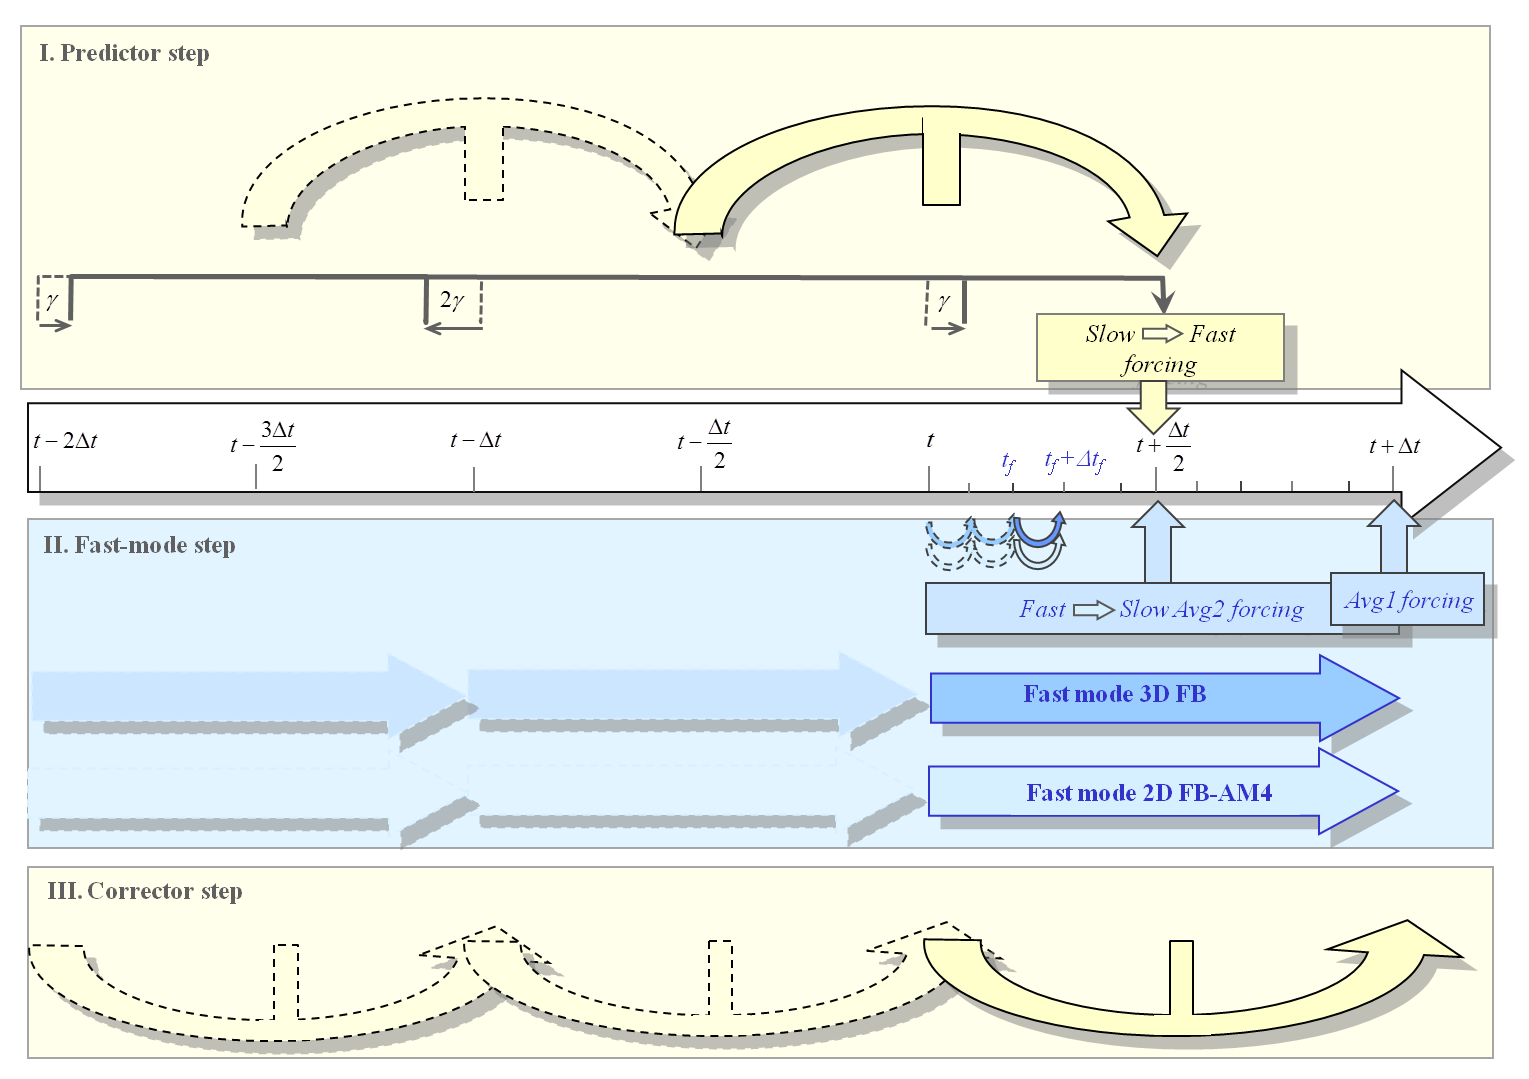
\includegraphics[width=1\linewidth]{CHAP2/Model_TS.png}
		\caption{}
	\end{subfigure}
\caption{ \textit{time-splitting and time-stepping of CROCO model with its non-hydrostatic, compressible (NBQ) kernel. Yellow (blue) background color: slow (fast) kernel. }}
	\label{ModelTS}
\end{figure}
%
\begin{table}
\begin{subequations}
\label{TimeSplit}
\begin{alignat}{3}
 \displaystyle
 %%%%%%%%%%%%%%%%%%%%%%%%%%%%%%%%%%%%%%%%%%%%%%%%%%%%%%%%%%%%%
 &\nonumber \textbf{I.a Time-interpolation: } t_s-\Delta t_s/2\\[0mm]
 %%%%%%%%%%%%%%%%%%%%%%%%%%%%%%%%%%%%%%%%%%%%%%%%%%%%%%%%%%%%%
 \label{TimeSplitIa1}
 &\enspace[\Theta] ^{n-\frac{1}{2}}=\alpha_{n-1}\Theta_s^{n-1}
 +\alpha_{n}\Theta_s^{n}\\[3mm]
 %%%%%%%%%%%%%%%%%%%%%%%%%%%%%%%%%%%%%%%%%%%%%%%%%%%%%%%%%%%%%
 &\nonumber \textbf{I.b Predictor step: } t_s+\Delta t_s/2\\[0mm]
 %%%%%%%%%%%%%%%%%%%%%%%%%%%%%%%%%%%%%%%%%%%%%%%%%%%%%%%%%%%%%
 \label{TimeSplitIb1}
 &\enspace\rho h\mathbf{v}_s^{n+\frac{1}{2}}=
 \rho h\mathbf{v}_s^{n-\frac{1}{2}}
 +\Delta t_s\left(\Lambda_{s,v}^{n}+<\Lambda_{f,v}>^n\right)\\[3mm]
 %
 \label{TimeSplitIb2}
 &\enspace\rho h(\theta_s,\ S_s)^{n+\frac{1}{2}}=
 \rho h(\theta_s,\ S_s)^{n-\frac{1}{2}}
 +\Delta t_s\Lambda_{s,(\theta,S)}^{n}\\[3mm]
 %
 \label{TimeSplitIb3}
 &\enspace\rho_s^{n+\frac{1}{2}}=\rho_{eos}\left(\theta_s^{n+\frac{1}{2}},\ S_s^{n+\frac{1}{2}},\ z_s^{n+\frac{1}{2}}\right)\\[3mm]
 %
 \label{TimeSplitIb4}
 &\enspace\partial_s\rho\omega_s^{n+\frac{1}{2}}=-\partial_t\rho h_s^{n+\frac{1}{2}}
 +\mathbf{\nabla}\cdot\rho h \mathbf{u}_s^{n+\frac{1}{2}}\\[3mm]
 %%%%%%%%%%%%%%%%%%%%%%%%%%%%%%%%%%%%%%%%%%%%%%%%%%%%%%%%%%%%%
 &\nonumber \textbf{I.c AB3-extrapolation: } t_s+\Delta t_s/2\\[0mm]
 %%%%%%%%%%%%%%%%%%%%%%%%%%%%%%%%%%%%%%%%%%%%%%%%%%%%%%%%%%%%%
 \label{TimeSplitIc1}
 &\enspace[[\Psi_s]]^{n+\frac{1}{2}}=
  \beta_{n-2}\Psi_s^{n-2}
 +\beta_{n-1}\Psi_s^{n-1}
 +\beta_{n}\Psi_s^{n}\\[2mm]
 %%%%%%%%%%%%%%%%%%%%%%%%%%%%%%%%%%%%%%%%%%%%%%%%%%%%%%%%%%%%%
 &\nonumber \textbf{II. Fast-mode steps: } t_f\in(t_s,\ t_s+\Delta t_s] \textit{ or } m\in[0,\ N_f)_\mathcal{N}\\[2mm]
 %%%%%%%%%%%%%%%%%%%%%%%%%%%%%%%%%%%%%%%%%%%%%%%%%%%%%%%%%%%%%
 \label{TimeSplitIIa}
 &\enspace\zeta_f^{m+1}=\zeta_f^{m}+\Delta t_f\left(
  w_{surf}^{m}-\mathbf{u}_{surf}^{m}.\mathbf{\nabla}\zeta^{m}\right)\\[2mm]
 %
 \label{TimeSplitIIb}
 &\enspace\rho h u_f^{m+1}=
 \rho h u_f^{m}
 +\Delta t_f\left(
  [[\Lambda_{s,u}]]^{n+\frac{1}{2}}
 -[[\overline{\Lambda_{s,u}}]]^{n+\frac{1}{2}}
 +\Lambda_{f,u}^{m}
% +\overline{\overline{\Lambda_{f,u}}}^{\ m}
 +\overline{\overline{\Lambda_{f,u}}}^{\ m}
 +\overline{\overline{\Lambda_{f,-\mathbf{\nabla}\zeta}}}^{\ m+1}
 \right)\\[2mm]
 %
 \label{TimeSplitIIc}
 &\enspace\overline{\overline{\rho h U}}_f^{\ m+1}=
 \overline{\overline{\rho h U}}_f^{\ m}
 +\Delta t_f\left(
 %[[\overline{\Lambda_{s,u}}]]^{n+\frac{1}{2}}+
 \overline{\Lambda_{f,u}^{m}}
 +\overline{\overline{\Lambda_{f,u}}}^{\ m}
 +\overline{\overline{\Lambda_{f,-\mathbf{\nabla}\zeta}}}^{\ m+1}
 \right)\\[0mm]
 %
 \label{TimeSplitIId}
 &\enspace\rho h w_f^{m+1}=
 \rho h w_f^{m}
 +\Delta t_f\left([[\Lambda_{s,w}]]^{n+\frac{1}{2}}
 +\Lambda_{f,w}^{m+1*}\right)\\[2mm]
 %
 \label{TimeSplitIIe}
 &\enspace\rho h_f^{m+1}=\rho h_f^{m}
 -\Delta t_f\left(
 [[\partial_t\rho h_s]]^{n+\frac{1}{2}}
 +\mathbf{\nabla}\cdot\{\rho h \mathbf{v}\}_f^{m+1}
 \right)\\[0mm]
 %
 \label{TimeSplitIIh}
 &\enspace m=N_f-1:\ \bar{\rho}\zeta_s^{n+1}
 =\bar{\rho}(H+\zeta_f)^{m}
 -\bar{\rho}H_s^{m+1}
 -\Delta t_f\mathbf{\nabla}\cdot\overline{\overline{\rho h\mathbf{u}}}^{\ m+1}\\[2mm]
 %
 \label{TimeSplitIIg}
 &\enspace \textit{Update\ grid:}\ \rho h_f^{m+1},\ z_f^{m+1}\\[2mm]
 %
 %%%%%%%%%%%%%%%%%%%%%%%%%%%%%%%%%%%%%%%%%%%%%%%%%%%%%%%%%%%%%
 &\nonumber \textbf{III.a Filtering: } t_s+\Delta t_s\ \textit{and}\ t_s+\Delta t_s/2\\[0mm]
 %%%%%%%%%%%%%%%%%%%%%%%%%%%%%%%%%%%%%%%%%%%%%%%%%%%%%%%%%%%%%
 \label{TimeSplitIIIa1}
 &\enspace<\Phi_f>^{n+1}=\Phi_f^{m=n+1}\\[0mm]
 \label{TimeSplitIIIa2}
 &\enspace\ll\Phi_f\gg^{n+\frac{1}{2}}=\frac{1}{N_f}\sum_{m=1}^{N_f}\Phi_f^{m}\\[2mm]
 %%%%%%%%%%%%%%%%%%%%%%%%%%%%%%%%%%%%%%%%%%%%%%%%%%%%%%%%%%%%%
 &\nonumber \textbf{III.b Corrector step: } t_s+\Delta t_s\\[0mm]
 %%%%%%%%%%%%%%%%%%%%%%%%%%%%%%%%%%%%%%%%%%%%%%%%%%%%%%%%%%%%%
 %
 \label{TimeSplitIIIb1}
 &\enspace\rho h\mathbf{v}_s^{n+1}=
 \rho h\mathbf{v}_s^{n}
 +\Delta t_s\left(\Lambda_s^{n+\frac{1}{2}*}
 +\ll\Lambda_f\gg^{n+\frac{1}{2}}\right)\\[0mm]
 %
 \label{TimeSplitIIIb2}
 &\enspace\partial_s\rho\omega_s^{n+1}=
 -\partial_{t\ }\rho h_s^{n+1}
 +\mathbf{\nabla}\cdot\rho h \mathbf{u}_s^{\ n+1}
 -\overline{\mathbf{\nabla}\cdot\rho h \mathbf{u}_s}^{\ n+1}
 -\overline{<\mathbf{\nabla}\cdot\rho h \mathbf{u}_s>}^{\ n+1}\\[2mm]
 %
 \label{TimeSplitIIIb3}
 &\enspace\rho h(\theta_s,\ S_s)^{n+1}=
 \rho h(\theta_s,\ S_s)^{n}
 +\Delta t_s\Lambda_{s,(\theta,S)}^{n+\frac{1}{2}*}\\[0mm]
 %
 \label{TimeSplitIIIb4}
 &\enspace\rho_s^{n+1}=\rho_{eos}\left(\theta_s^{n+1},\ S_s^{n+1},\ z_s^{n+1}\right)\\[0mm]
 %
 \label{TimeSplitIIIb5}
 &\enspace\rho h\mathbf{u}_s^{n+1}=\rho h\mathbf{u}_s^{n+1}
 -\overline{\rho h\mathbf{u}_s}^{\ n+1}
 +\overline{\rho h\mathbf{u}_f}^{\ m=N_f-1}
 %%%%%%%%%%%%%%%%%%%%%%%%%%%%%%%%%%%%%%%%%%%%%%%%%%%%%%%%%%%%%
\end{alignat}
\end{subequations}
\end{table}
Predictor (I), fast-kernel Forward-Backward (II) and Corrector (III) steps are shown in horizontal color bands on figure \ref{ModelTS} (yellow for the slow kernel, blue for the fast kernel). After time-interpolating slow-kernel variables to $t_s-\Delta t_s/2$ (step I.a, notation $[.]$), the slow kernel is advanced from $t_s-\Delta t_s/2$ to $t_s+\Delta t_s/2$ with a centered, leap-frog-like, time-stepping (step I.b). Then, to prepare the integration of the fast kernel, the slow-kernel RHS is extrapolated to $t_s+\Delta t_s/2$ based on an AB3 scheme using its previous evaluations at $t_s-2\Delta t_s$, $t_s-\Delta t_s$ and $t_s$ (step I.c, notation $[[.]]$). The fast kernel can in turn be advanced from $t_s$ to $t_s+\Delta t_s$ using a forward-backward like time-stepping (step II) with time-step $\Delta t_f$ satisfying  $N_f=\Delta t_s/\Delta t_f\in\mathcal{N}$. The vertical momentum equation can optionaly be integrated with semi-implicit scheme over the vertical direction.\\ 
The vertical grid is updated at each fast time-step \ref{TimeSplitIIg} but slow-kernel components of the RHS remain constant during the fast-kernel integration. At the last fast time-step, surface elevation displacement for the slow kernel can be recomputed to ensure perfect numerical coherence between the surface kinematic relation and depth-integrated mass conservation (\noparref{TimeSplitIIa} and \noparref{TimeSplitIIh}).\\
Further numerical details such as the values of the interpolation $(\alpha_n)$ or extrapolation $(\beta_n)$ coefficients, the expressions of the slow-kernel RHS terms $(\Lambda_s)$, the expressions of the fast-kernel surface-related pressure force terms $(\Lambda_{f,-\nabla\zeta})$,  the fast-kernel RHS remaining terms $(\Lambda_{f})$ or the implicit fast and slow-kernel RHS terms (indicated by an asterisk) can be found in CROCO dedicated manuals and publications.\\  
%The barotropic-like, depth-independent component is also integrated with the same time-step $\Delta t_f$ with a forward-backward scheme as in \cite{shchepetkin_regional_2005}. 
A major difference with the hydrostatic time-splitting is that the surface elevation displacement is given by the kinematic condition \ref{TimeSplitIIa} and not by the depth-integral of the mass conservation equation. Once the fast-kernel RHS and variables have been filtered both at $t_s+\Delta t_s$ and $t_s+\Delta t_s/2$ (step III.a, notations $<.>$ and $\ll.\gg$), the slow kernel is finally advanced from $t$ to  $t_s+\Delta t_s$ during the leap-frog-like Corrector step (III.b). A star following the time-index superscript indicates the use of an implicit numerical schemes.

Note that the 2D depth-averaged, barotropic-like, horizontal momentum equations (double over-bar notation) \ref{TimeSplitIIc} are advanced in the same way as in \cite{shchepetkin_regional_2005}. The result of this 2D integration is indeed used to correct both the horizontal momentum itself and the RHS of the horizontal momentum equation at Corrector step. It can also be used to require a perfect coherence of the surface elevation displacement and the depth-average transport (at machine precision) during the slow-mode integration.

\color{blue}
\section{Conclusion, discussion of the \textit{ocean model}}
In the present chapter, we proposed a rigorous framework (an "map") for our exploration of ocean \textit{fine scales} in \textit{Terra Incognita}. An analytical, terrain-following s-coordinate model for the conservation of mass, momentum, heat and tracers has first been proposed under general assumptions of a compressible, free-surface ocean (\S \noparref{section_prim_eq}). \\
%An original derivation (to our knowledge) of the evolution of the potential energy of a free-surface column of fluid has been carried out.\\%FA%
We then considered the numerical implementation of this general \textit{ocean model} (\S \noparref{section_croco}). After a consideration of the space-time scales potentially involved in the fine scale ocean dynamics, an original time-splitting has been detailed as an extension of \cite{shchepetkin_regional_2005}'s barotropic/baroclinic time-splitting. It is also a restriction to a two-mode time-splitting of \cite{Auclair2018}'s three-mode time-splitting. This time-splitting allows the integration of both acoustic and surface-induced processes with a smaller time-step in order to make the integration of a compressible, free-surface realistic ocean affordable. It is based on the spectral gaps identified in \ref{velocityscales} between acoustic, surface and internal processes.\\
The region of Gibraltar strait has been chosen as the region of demonstration for its fine-scale dynamics. As a consequence, the LES configurations presented in chapters \ref{chapGBR2D}, \ref{chapGBR3D} and \ref{chapBPE} are not only based on the resulting two-mode CROCO kernel but these configurations have thus been part of the development process itself. 
%The investigation of mixing in real-ocean conditions proposed in chapter \ref{chapBPE} takes roots in the general evolution equation of potential energy proposed in (\S \noparref{section_prim_eq}).
\color{black}
%%%%%%%%%%%%%%%%%%%%%%%%%%%%%%%%%%%%%%%%%%%%%%%%%%%%%%%%%%%%%%%%%%%%%%%%%%%
%%%%%%%%%%%%%%%%%%%%%%%%%%%%%%%%%%%%%%%%%%%%%%%%%%%%%%%%%%%%%%%%%%%%%%%%%%%
%%%%%%%%%%%%%%%%%%%%%%%%%%%%%%%%%%%%%%%%%%%%%%%%%%%%%%%%%%%%%%%%%%%%%%%%%%%
\section{Appendices to the \textit{ocean model}}
\label{annexe_ocmod}
%%%%%%%%%%%%%%%%%%%%%%%%%%%%%%%%%%%%%%%%%%%%%%%%%%%%%%%%%%%%%%%%%%%%%%%%%%%
%%%%%%%%%%%%%%%%%%%%%%%%%%%%%%%%%%%%%%%%%%%%%%%%%%%%%%%%%%%%%%%%%%%%%%%%%%%
%%%%%%%%%%%%%%%%%%%%%%%%%%%%%%%%%%%%%%%%%%%%%%%%%%%%%%%%%%%%%%%%%%%%%%%%%%%

\subsection{$s$-coordinate transformation}
\label{section_annexe2}
The present appendix gathers several formula and relations essential to the development of the numerical implementation of the \textit{ocean model}.
%
%%%%%%%%%%%%%%%%%%%%%%%%%%%%%%%%%%%%%%%%%%%%%%%%%%%%%%%%%%%%%%%%%%%%%%%%%%%%%
\subsubsection{Transformation matrices}
\label{annexe_coordS}
%%%%%%%%%%%%%%%%%%%%%%%%%%%%%%%%%%%%%%%%%%%%%%%%%%%%%%%%%%%%%%%%%%%%%%%%%%%%%
The transformation matrix of the generalized coordinate transformation is:
\begin{equation}
    \displaystyle
    \Lambda^z_s=
    \begin{pmatrix}
    1 & 0 & 0 & 0 \\
    0 & 1 & 0 & 0 \\
    0 & 0 & 1 & 0 \\
    \frac{\partial z}{\partial t} & \frac{\partial z}{\partial x}
    & \frac{\partial z}{\partial y} & h=\frac{\partial z}{\partial s}
    \end{pmatrix}
\end{equation}
and the inverse transformation is given by:
\begin{equation}
    \displaystyle
    \Lambda_z^s=
    \begin{pmatrix}
    1 & 0 & 0 & 0 \\
    0 & 1 & 0 & 0 \\
    0 & 0 & 1 & 0 \\
    \frac{\partial s}{\partial t} & \frac{\partial s}{\partial x}
    & \frac{\partial s}{\partial y} & \frac{\partial s}{\partial z}
    \end{pmatrix}
\end{equation}
The Jacobian of the transformation $J=det(\Lambda^z_s)$ is the (specific) thickness:
\begin{equation}
 \displaystyle
 J=h=\frac{\partial z}{\partial s}=\frac{\partial z}{\partial s}\bigg\vert_{xyt}
\end{equation}
\cite{griffies_fundamentals_2004} further define the infinitesimal  thickness for modelling developments:
\begin{equation}
 \displaystyle
 \delta h=\frac{\partial z}{\partial s} \delta s
\end{equation}

%%%%%%%%%%%%%%%%%%%%%%%%%%%%%%%%%%%%%%%%%%%%%%%%%%%%%%%%%%%%%%%%%%%%%%%%%%%%%
\subsubsection{Formula and identities}
%%%%%%%%%%%%%%%%%%%%%%%%%%%%%%%%%%%%%%%%%%%%%%%%%%%%%%%%%%%%%%%%%%%%%%%%%%%%%
Base on the transformation matrices, the $s$-coordinate transformations can be rewritten:
\begin{subequations}
  \begin{alignat}{2}
  \displaystyle 
  &\frac{\partial A}{\partial t}\bigg\rvert_{xz} &&=
   \frac{\partial A}{\partial t}\bigg\rvert_{xs}
  - \frac{1}{h} \frac{\partial A}{\partial s}\bigg\rvert_{tx}
  \frac{\partial z}{\partial t}\bigg\rvert_{xs}\\[4mm]
  &\frac{\partial A}{\partial x}\bigg\rvert_{tz} &&=
   \frac{\partial A}{\partial x}\bigg\rvert_{ts}
  - \frac{1}{h} \frac{\partial A}{\partial s}\bigg\rvert_{tx}
  \frac{\partial z}{\partial x}\bigg\rvert_{ts}\\[4mm]
  &\frac{\partial A}{\partial z}\bigg\rvert_{tx} &&=
   \frac{1}{h}
   \frac{\partial A}{\partial s}\bigg\rvert_{tx}
  \end{alignat}
\end{subequations}
whereas material derivatives satisfy:
\begin{subequations}
  \begin{alignat}{2}
  \displaystyle 
  & \frac{d}{dt} &&=\frac{\partial}{\partial t}\bigg\vert_z
  + \mathbf{u}.\mathbf{\nabla}_z
  + w\frac{\partial }{\partial z}\\[4mm]
  & &&=\frac{\partial}{\partial t}\bigg\vert_s
  + \mathbf{u}.\mathbf{\nabla}_s
  + \dot{s}\frac{\partial}{\partial s}
  \end{alignat}
\end{subequations}
This leads to:
\begin{equation}
  \displaystyle 
  \dot{z} =\frac{dz}{dt}\bigg\vert_s=\frac{\partial z}{\partial t}\bigg\vert_s
  + \mathbf{u}.\mathbf{\nabla}_s z
  + \dot{s}\frac{\partial z}{\partial s},\quad r\quad
  \dot{s} =\frac{ds}{dt}\bigg\vert_z=\frac{\partial s}{\partial t}\bigg\vert_z
  + \mathbf{u}.\mathbf{\nabla}_z s
  + w\frac{\partial s}{\partial z}
\end{equation}
Using the identities:
\begin{equation}
  \displaystyle
  \frac{\partial s}{\partial t}\bigg\vert_z =
  \left(\frac{\partial t}{\partial s}\bigg\vert_z\right)^{-1},\quad
  \frac{\partial s}{\partial x}\bigg\vert_z =
  \left(\frac{\partial x}{\partial s}\bigg\vert_z\right)^{-1},\quad
  \frac{\partial s}{\partial y}\bigg\vert_z =
  \left(\frac{\partial y}{\partial s}\bigg\vert_z\right)^{-1},\quad
  \frac{\partial s}{\partial z}\bigg\vert_x =
  \left(\frac{\partial z}{\partial s}\bigg\vert_x\right)^{-1
\end{equation}
several relations can be obtained from the triple product rule and the coordinate transformations are given by:
\begin{equation}
  \displaystyle
  \frac{\partial z}{\partial t}\bigg\vert_s =
  -\frac{\partial s}{\partial t}\bigg\vert_z\frac{\partial z}{\partial s}\bigg\vert_s,\quad
  \frac{\partial z}{\partial x}\bigg\vert_s =
  -\frac{\partial s}{\partial x}\bigg\vert_z\frac{\partial z}{\partial s}\bigg\vert_s,\quad
  \frac{\partial z}{\partial y}\bigg\vert_s =
  -\frac{\partial s}{\partial y}\bigg\vert_z\frac{\partial z}{\partial s}\bigg\vert_s\\
\end{equation}

%%%%%%%%%%%%%%%%%%%%%%%%%%%%%%%%%%%%%%%%%%%%%%%%%%%%%%%%%%%%%%%%%%%%%%%%%%%%%
\subsubsection{Local orthonormal coordinates}
%%%%%%%%%%%%%%%%%%%%%%%%%%%%%%%%%%%%%%%%%%%%%%%%%%%%%%%%%%%%%%%%%%%%%%%%%%%%%
\cite{griffies_fundamentals_2004} further defines in his chapter (6.4) a system of orthonormal coordinates:
\begin{equation}
  \displaystyle 
  \mathbf{e}_{x^*} =\frac{\mathbf{y}\wedge{\mathbf{\nabla}s}}
  {\norm{\mathbf{y}\wedge{\mathbf{\nabla}s}}},\quad
  \mathbf{e}_{y^*} =\mathbf{e}_s\wedge{\mathbf{e}_{x^*}},\quad
  \mathbf{e}_s =\frac{\mathbf{\nabla}s}{\norm{\mathbf{\nabla}s}}
\end{equation}
In this particular case ($\mathbf{e}_s.\mathbf{z}$) has a unique sign, the basis vectors can be rewritten:
\begin{equation}
  \displaystyle 
  \mathbf{e}_{x^*} =\frac{\mathbf{x}+S_x\mathbf{z}}{\sqrt{1+S_x^2}},\quad
  \mathbf{e}_{y^*} =\frac{-S_xS_y\mathbf{x}+(1+S_x^2)\mathbf{y}+S_y\mathbf{z}}{\sqrt{1+S^2)(1+S_x^2)}},\quad
  \mathbf{e}_s =\frac{(-\mathbf{S},1)}{\sqrt{1+S^2}}
\end{equation}
The s-coordinate transformation is a rotation and:
\begin{equation}
   \displaystyle
   \mathbf{e}_{x^*y^*s}=\Lambda_{s}^{z}\mathbf{e}_{xyz}
\end{equation}
Note in particular the definition of the slope $\mathbf{S}$ and its norm $S=\norm{\mathbf{S}}$ used to rewrite the orthonormal basis:
\begin{equation}
   \displaystyle
   \mathbf{S}=\mathbf{\nabla}_s z=
   -\frac{\partial z}{\partial s}\mathbf{\nabla}_z s=\left( S_x,\ S_y,\ 0 \right)
\end{equation}
where $\mathbf{\nabla}_s z$ is "the horizontal gradient of the height of a fluid parcel as taken along surfaces of constant generalized vertical coordinate s" \citep{griffies_fundamentals_2004}.

Note that this orthonormal basis is not used to project the equations of the model. S-coordinates are "only" used as a change of variable whereas equations and vector quantities remain written in the original Cartesian or spherical basis. The present s-coordinate orthonormal basis is presented here to be latter used in the computation of fluxes through s-surfaces.


%%%%%%%%%%%%%%%%%%%%%%%%%%%%%%%%%%%%%%%%%%%%%%%%%%%%%%%%%%%%%%%%%%%%%%%%%%%%%
\subsection{Operators \& relations in s-coordinates}
\label{annexe_s-coord}
%%%%%%%%%%%%%%%%%%%%%%%%%%%%%%%%%%%%%%%%%%%%%%%%%%%%%%%%%%%%%%%%%%%%%%%%%%%%%

%%%%%%%%%%%%%%%%%%%%%%%%%%%%%%%%%%%%%%%%%%%%%%%%%%%%%%%%%%%%%%%%%%%%%%%%%%%%%
\subsubsection{Divergence of the velocity field in s-coordinates}
%%%%%%%%%%%%%%%%%%%%%%%%%%%%%%%%%%%%%%%%%%%%%%%%%%%%%%%%%%%%%%%%%%%%%%%%%%%%%
Using :
\begin{equation}
 \displaystyle
 \frac{\partial}{\partial t} \frac{\partial z}{\partial s}\bigg\vert_{tx}= \frac{\partial h}{\partial t} \qquad and \qquad \frac{\partial}{\partial x} \frac{\partial z}{\partial s}\bigg\vert_{tx}= \frac{\partial h}{\partial x}
\end{equation}
%and
%\begin{equation}
% \displaystyle
% \frac{\partial}{\partial x} \frac{\partial z}{\partial s}\bigg\vert_{tx}= \frac{\partial h}{\partial x}
%\end{equation}
%
the expression of the divergence of the velocity field in s-coordinates can be written:
\begin{subequations}
  \begin{alignat}{2}
  & h \ \mathbf{\nabla}.( \mathbf v) &&= h \frac{\partial u}{\partial x} \bigg \rvert_{zt} +h \frac{\partial v_z}{\partial z} \bigg \rvert_{xt}\\[4mm]
  & && = h \frac{\partial u}{\partial x} \bigg \rvert_{st} - \frac{h}{h} \frac{\partial u}{\partial s}\bigg \rvert_{tx} \frac{\partial z}{\partial x}\bigg \rvert_{ts}
  \quad + \frac{h}{h}  \frac{\partial}{\partial s} \bigg ( v_s + \frac{\partial z }{\partial t}\bigg \rvert_{xs} + u \frac{\partial z}{\partial x}\bigg \rvert_{ts} \bigg )\\[4mm]
  & && = h \frac{\partial u}{\partial x} \bigg \rvert_{st} -  \frac{\partial u}{\partial s}\bigg \rvert_{tx} \frac{\partial z}{\partial x}\bigg \rvert_{ts} 
  \quad +  \frac{\partial v_s}{\partial s} +  \frac{\partial h}{\partial t} + u \frac{\partial h}{\partial x} + \frac{\partial u}{\partial s}\bigg \rvert_{tx} \frac{\partial z}{\partial x}\bigg \rvert_{ts}\\[4mm]
  & && = \frac{\partial v_s}{\partial s}\bigg \rvert_{tx} + \frac{\partial h u}{\partial x} \bigg \rvert_{ts}+ \frac{\partial h}{\partial t}\bigg \rvert_{xs}
  \end{alignat}
\end{subequations}
Note that this is a particular case of the formulation of a change of variables with its Jacobian ($J=h$ in the present case). %This leads to several useful conservative formulations in the following section.
%
%%%%%%%%%%%%%%%%%%%%%%%%%%%%%%%%%%%%%%%%%%%%%%%%%%%%%%%%%%%%%%%%%%%%%%%%%%%%%
\subsubsection{Conservative "flux" forms: kinematics \& dynamics}
%%%%%%%%%%%%%%%%%%%%%%%%%%%%%%%%%%%%%%%%%%%%%%%%%%%%%%%%%%%%%%%%%%%%%%%%%%%%%
Two general conservative formulations can be obtained combining this with the continuity equation \citep{auclair_woceanfr_2011}\footnote{WOcean.fr Web Site: \url{http://poc.omp.obs-mip.fr/auclair/WOcean.fr/SNH/Restricted/NH-NBQ/Sources/Images/png/Coord_demo.png}\label{WOcean_scoord}}.

$A$ is a property given per unit mass (thermodynamically intensive) (see the demonstration on web site). The first two (conservative) relations are fundamentals to analytical and numerical modeling.


\textbf{\textit{Based on the conservation of mass:}}
\begin{equation}
  \displaystyle 
  \rho \frac{d A}{dt}
  =\frac{\partial \rho A}{\partial t}\bigg\rvert_{xz}
  +\frac{\partial \rho A u}{\partial x}\bigg\rvert_{tz}
  +\frac{\partial \rho  v_s}{\partial z}\bigg\rvert_{tx}
\end{equation}

\textbf{\textit{Based on the conservation of mass \& in s-coordinates:}}
\begin{equation}
  \displaystyle 
  \rho h \frac{d A}{dt}
  =\frac{\partial \rho h A}{\partial t}\bigg\rvert_{xs}
  +\frac{\partial \rho h A u}{\partial x}\bigg\rvert_{ts}
  +\frac{\partial \rho  A v_s}{\partial s}\bigg\rvert_{tx}
\end{equation}
\textbf{\textit{A kinematic, non-conservative formulation}} can be obtained without the continuity equation:
\begin{equation}
\frac{d A}{d t} = \frac{\partial A}{\partial t} \bigg\rvert_{xs} + u \frac{\partial A}{\partial x} \bigg\rvert_{ts} + \frac{v_s}{h}\frac{\partial A}{\partial s}\bigg\rvert_{tx}
\end{equation}
The demonstration is given in \citep{auclair_woceanfr_2011}$^{\noparref{WOcean_scoord}}$.\\

\textbf{\textit{Conservation of mass:}}
note finally that the conservation of mass $A=1$ can then be rewritten:
\begin{equation}
  \displaystyle 
  \label{mass_s}
  h\frac{d\rho}{d t}
  =\frac{\partial \rho h }{\partial t}\bigg\rvert_{xs}
  +\frac{\partial \rho h u}{\partial x}\bigg\rvert_{ts}
  +\frac{\partial \rho  v_s}{\partial s}\bigg\rvert_{tx}
\end{equation}

Additionnally, the evolution of $\rho$ in equation \ref{eq_diff_cart} can be rewritten in s-coordinates as:
\begin{equation}
\label{eq_diff_s}
\displaystyle
h \frac{d \rho }{d t} \approx
\frac{\partial}{\partial x} \bigg(h \kappa^h \frac{\partial \rho}{\partial x}\bigg\rvert_{ts}\bigg)_{ts}
+ \frac{\partial}{\partial s} \bigg(\frac{\kappa^v}{h} \frac{\partial \rho}{\partial s}\bigg\rvert_{tx}\bigg)_{tx} 
\end{equation}
with: $\kappa_c^h \approx \kappa^h$ and $\kappa_c^v \approx \kappa^v$.\\






\chapter{GBR2D}
\begin{itemize}
\item R\'esum\'e en français
\item Papier 2D (! Changer numero de page pour debut pdf !, et retirer biblio (avec en fin these....), mise en page verifier...(problème tableau 2))
\item Recap/clsion/transition français
\end{itemize}

\section{Resumé en français}
\begin{itemize}
\item blabla détroit Gibraltar, pourquoi choisi cette zone, résumé intro papier
\item mise en place configuration, résolution, non hydrostatique...
\item résultats : a bien solitons (aspect, KdV), controle hydraulique, voit des rouleaux = instabilités primaires (confirmation)
\end{itemize}

CE chapitre contient l'artcile "..." publié dans ... .CErtains des éléments de cet article, l'élaboration du processus de 
certaisn éléments d'analyse de cette configuration ont été ralisés entière ment ou au moins améliorés dans la première année de thèse, c'ets le cas de l'analyse en composante principake des instabilités primaire sdéveloppées...etc.


Une configuration numérique simple 2D est implémentée dans le détroit de Gibraltar avec le code communautaire CROCO dans sa version non-hydrostatique, non-Boussinesq (CROCO-NBQ). Cette configuration est peu coûteuse en temps de calcul et incorpore la bathymétrie le long de l'axe du détroit avec sa configuration de seuils (Farmer et Armi, 1988, programme \textit{Gibraltar Experiment}). Dans l'élaboration de cette configuration, une attention toute particulière a été apportée au rôle de la pseudo-force de Coriolis sur l'échange moyen simulé lors de l'initialisation par \textit{lock-exchange}.\\

LA simulation est initialisée par lock exhange, c'est à dire un profil type atl et med de part et d'autre du seuil de camarinal, point central du passage.LA marée est simulée par un courant barotrope à la frontière ouest. Dans une simulation où la rotation de la terre n'est pas rise en compte, mélange détruit stratification obtenue apres relâchement du lock exhange, en particulier la profondeur de l'interface où se propagent les solitons, suite au mélange intense par la marée interne.


Malgré les défauts inhérents à une représentation 2D-verticale (nécessairement limitée dynamiquement et non représentative des effets longitudinaux comme le contrôle dans le détroit de Tarifa), la configuration proposée permet de représenter de façon réaliste les mécanismes de \textit{fine échelle} dans le détroit à la fréquence de la marée barotrope : propagation des deux premiers modes d'ondes internes, contrôles hydrauliques aux seuils, ressaut hydraulique, et mélange turbulent. En particulier, les ondes internes de grande amplitude de mode 1 se propageant dans l'est du détroit sont caractérisées comme ondes solitaires (ou solitons) par comparaison avec le modèle analytique non-linéaire de Korteweig de Vries.\\

La modulation des phénomènes observés par divers paramètres (bathymétrie, intensité des courants de marée, hypothèse hydrostatique, résolution spatiale) est étudiée en détail. A haute résolution (environ 45 m), la relaxation de l'hypothèse non-hydrostatique est indispensable pour représenter les instabilités de cisaillement qui apparaissent dans le jet Méditerranéen, et qui constituent l'amorce de la cascade turbulente directe.



%%%%PAPIER 2D%%%%%%%%%%%%%%%%%%%%%%%%%%%%%%%%%%%%%%%%
%voir si faut mettre pdf envoye ou quoi.... mise en forme abstract, key words, auteurs...
%%% faut le mettre en section seul sans les plus petits titres...
%%numerotation...
%\newpage
%%%%%%%%%%%%%%%%%%%%%%%%%%%%%%%%%%%%%%%%%%%%%%%%%%%%%%%%%%%%%%%%%%%%%%%%%%%%
%   Manuscrit these
%%%%%%%%%%%%%%%%%%%%%%%%%%%%%%%%%%%%%%%%%%%%%%%%%%%%%%%%%%%%%%%%%%%%%%%%%%%

%%%%%%%%%%%%%%%%%%%%%%%%%%%%%%%%%%%%%%%%%%%%%%%%%%%%%%%%%%%%%%%%%%%%%%%%
\documentclass[a4paper,12pt,notitlepage]{report}
%%%%%%%%%%%%%%%%%%%%%%%%%%%%%%%%%%%%%%%%%%%%%%%%%%%%%%%%%%%%%%%%%%%%%%%%%%%

%%%%%%%%%%%%%%%%%%%%%%%%%%%%%%%%%%%%%%%%%%%%%%%%%%%%%%%%%%%%%%%%%%%%%%%%%%%
% Packages
%%%%%%%%%%%%%%%%%%%%%%%%%%%%%%%%%%%%%%%%%%%%%%%%%%%%%%%%%%%%%%%%%%%%%%%%%%%

\usepackage[a4paper,top=1.5cm,bottom=2cm,left=2.5cm,right=2.5cm,marginparwidth=1.75cm]{geometry}
\usepackage{graphicx} 
\usepackage[hidelinks]{hyperref} 
\usepackage{multirow} 
\usepackage{tabularx} 
\usepackage{color} 
\usepackage[fleqn]{amsmath}
\usepackage{amsfonts}
\usepackage{amssymb}
\usepackage{textcomp}
\usepackage{gensymb}
\usepackage{array}
\usepackage{amsxtra} 
\usepackage{wasysym} 
\usepackage{isomath} 
\usepackage{mathtools} 
\usepackage{txfonts} 
\usepackage{upgreek} 
\usepackage{enumerate} 
\usepackage{tensor} 
\usepackage{pifont} 
\usepackage{titlesec}
\usepackage[utf8x]{inputenc}
\usepackage[T1]{fontenc}
\usepackage{fancyhdr}
\usepackage{enumitem}
%\usepackage[colorlinks=true, allcolors=blue]{hyperref}
\usepackage{subcaption}
\usepackage[normalem]{ulem} %25/05 Barrer un texte.
\usepackage{caption}        %04/06
\usepackage{afterpage}      %04/6
\usepackage{geometry}       %05/06
%\usepackage{wrapfig}        %04/06
\usepackage{float}
%\usepackage[printfigures]{endfloat}
%\usepackage{endfloat}
%\usepackage{subfig}
%\usepackage{graphicx}
%package floatend
\usepackage{booktabs}
\usepackage{appendix}
%\usepackage{array, makecell}
%\renewcommand\theadfont{\bfseries}
%\usepackage{esint}
\usepackage{cancel}
%\usepackage{pdfpages}
%----------------------------------------------------------------------------
% Packages: uncomment to debug
%----------------------------------------------------------------------------
%\usepackage{refcheck}
%\renewcommand{\labelitemi}{\textbullet}

%----------------------------------------------------------------------------
% Packages: bibliography
%----------------------------------------------------------------------------
\usepackage[nottoc, notlof, notlot]{tocbibind}
%\usepackage[authoryear, round]{natbib}
\usepackage[authoryear]{natbib}
%\usepackage[frenchb]{babel}
%\usepackage{authblk}

%%%%%%%%%%%%%%%%%%%%%%%%%%%%%%%%%%%%%%%%%%%%%%%%%%%%%%%%%%%%%%%%%%%%%%%%%%%
% Definitions & commands
%%%%%%%%%%%%%%%%%%%%%%%%%%%%%%%%%%%%%%%%%%%%%%%%%%%%%%%%%%%%%%%%%%%%%%%%%%%

%----------------------------------------------------------------------------
% New operators
%----------------------------------------------------------------------------
\DeclareMathOperator{\cotan}{cotan}

%----------------------------------------------------------------------------
% New commands
%----------------------------------------------------------------------------
\newcommand{\nhi}[1]{%
	{\itshape \color{magenta} (NHI approx: {#1})}}
\newcommand{\hi}[1]{%
	{\itshape \color{cyan} (HI approx: {#1})}}

%----------------------------------------------------------------------------
\setlength\parindent{0pt}
%----------------------------------------------------------------------------

%----------------------------------------------------------------------------
% Colors...
%----------------------------------------------------------------------------
\definecolor{color-1}{rgb}{0.21,0.37,0.57}
\definecolor{color-2}{rgb}{0.31,0.51,0.74}

%----------------------------------------------------------------------------
\geometry{hmargin=2.5cm,vmargin=2.5cm} %marges
%----------------------------------------------------------------------------

\renewcommand{\thepage}{}
\renewcommand{\thepage}{\arabic{page}}

\newcommand\norm[1]{\left\lVert#1\right\rVert}

\numberwithin{equation}{section}


%%%%%%%%%%%%%%%%%%%%%%%%%%%%%%%%%%%%%%%%%%%%%%%%%%%%%%%%%%%%%%%%%%%%%%%%%%%%%
\begin{document}
%%%%%%%%%%%%%%%%%%%%%%%%%%%%%%%%%%%%%%%%%%%%%%%%%%%%%%%%%%%%%%%%%%%%%%%%%%%%%

\hypersetup{pdfborder=0 0 0}%----------------------------------------------------------------------------
% \ref with or without ( )
%----------------------------------------------------------------------------
\let\noparref\ref
\renewcommand{\ref}[1]{(\noparref{#1})}

\setcounter{tocdepth}{3}%1 juste 1 niveau sous-partie de chapitre

Inclure pdf page de titre

\newpage
\textbf{Avant-propos et remerciements}
\addcontentsline{toc}{section}{Avant-propos et remerciements}
\newpage
%%%%%%%%%%%%%%%%%%%%%%%%%%%%%%%%%%%%%%%%%%%%%%%%%%%%%%%%%%%%%%%%%%%%%%%%%%%%%
\tableofcontents

%%%%%%%%%%%%%%%%%%%%%%%%%%%%%%%%%%%%%%%%%%%%%%%%%%%%%%%%%%%%%%%%%%%%%%%%%%%%%

\newpage
\chapter{Introduction}
%\cite{BS84}
\citet{armi_1985}


\input{./INTRO/intro.tex}

%%%%%%%%%%%%%%%%%%%%%%%%%%%%%%%%%%%%%%%%%%%%%%%%%%%%%%%%%%


\chapter{Mod\'elisation  Repr\'esentation de l'oc\'ean et de son m\'elange}
\begin{itemize}
\item conservation masses/qdm, discretisation numérique, échelles (RANS/LES(/DNS)), paramétrisation du mélange, fermeture turb (Smago/GLS...)
\item contenu en PV
\item definition BPE, eq d'évolution 'générale'
\item code CROCO (ou code CROCO en premisce de chap 3 GBR2D????(sinon parait cours?)GBR2D parle passage hydro a NBQ...)
\end{itemize}


\input{./CHAP2/chap2.tex}





\chapter{GBR2D}
\begin{itemize}
\item R\'esum\'e en français
\item Papier 2D (! Changer numero de page pour debut pdf !, et retirer biblio (avec en fin these....), mise en page verifier...(problème tableau 2))
\item Recap/clsion/transition français
\end{itemize}

\section{Resumé en français}
\begin{itemize}
\item blabla détroit Gibraltar, pourquoi choisi cette zone, résumé intro papier
\item mise en place configuration, résolution, non hydrostatique...
\item résultats : a bien solitons (aspect, KdV), controle hydraulique, voit des rouleaux = instabilités primaires (confirmation)
\end{itemize}

CE chapitre contient l'artcile "..." publié dans ... .CErtains des éléments de cet article, l'élaboration du processus de 
certaisn éléments d'analyse de cette configuration ont été ralisés entière ment ou au moins améliorés dans la première année de thèse, c'ets le cas de l'analyse en composante principake des instabilités primaire sdéveloppées...etc.


Une configuration numérique simple 2D est implémentée dans le détroit de Gibraltar avec le code communautaire CROCO dans sa version non-hydrostatique, non-Boussinesq (CROCO-NBQ). Cette configuration est peu coûteuse en temps de calcul et incorpore la bathymétrie le long de l'axe du détroit avec sa configuration de seuils (Farmer et Armi, 1988, programme \textit{Gibraltar Experiment}). Dans l'élaboration de cette configuration, une attention toute particulière a été apportée au rôle de la pseudo-force de Coriolis sur l'échange moyen simulé lors de l'initialisation par \textit{lock-exchange}.\\

LA simulation est initialisée par lock exhange, c'est à dire un profil type atl et med de part et d'autre du seuil de camarinal, point central du passage.LA marée est simulée par un courant barotrope à la frontière ouest. Dans une simulation où la rotation de la terre n'est pas rise en compte, mélange détruit stratification obtenue apres relâchement du lock exhange, en particulier la profondeur de l'interface où se propagent les solitons, suite au mélange intense par la marée interne.


Malgré les défauts inhérents à une représentation 2D-verticale (nécessairement limitée dynamiquement et non représentative des effets longitudinaux comme le contrôle dans le détroit de Tarifa), la configuration proposée permet de représenter de façon réaliste les mécanismes de \textit{fine échelle} dans le détroit à la fréquence de la marée barotrope : propagation des deux premiers modes d'ondes internes, contrôles hydrauliques aux seuils, ressaut hydraulique, et mélange turbulent. En particulier, les ondes internes de grande amplitude de mode 1 se propageant dans l'est du détroit sont caractérisées comme ondes solitaires (ou solitons) par comparaison avec le modèle analytique non-linéaire de Korteweig de Vries.\\

La modulation des phénomènes observés par divers paramètres (bathymétrie, intensité des courants de marée, hypothèse hydrostatique, résolution spatiale) est étudiée en détail. A haute résolution (environ 45 m), la relaxation de l'hypothèse non-hydrostatique est indispensable pour représenter les instabilités de cisaillement qui apparaissent dans le jet Méditerranéen, et qui constituent l'amorce de la cascade turbulente directe.



%%%%PAPIER 2D%%%%%%%%%%%%%%%%%%%%%%%%%%%%%%%%%%%%%%%%
%voir si faut mettre pdf envoye ou quoi.... mise en forme abstract, key words, auteurs...
%%% faut le mettre en section seul sans les plus petits titres...
%%numerotation...
%\newpage
%\input{./GBR2D/main.tex}
%\newpage
%%%% En mettant PDF
%%%mettre autre pdf avec figure incluse aux bons endroits etc...
\addtocounter{section}{1}
\addcontentsline{toc}{section}{\protect\numberline{\thesection}Papier 2D}
%\includepdf[pages=-]{./GBR2D/PDF_GBR2D.pdf}%%!!attention decommenter package



\section{ccl français}
\begin{itemize}
\item Limitation de la simulations 2D, transition partie 3D
\end{itemize}


%%%%%%%%%%%%%%%%%%%%%%%%%%%%%%%%%%%%%%%%%%%%%%%%%%%%%%%%%%

\chapter{GBR3D}



%%\selectlanguage{english}
\input{./GBR3D/chapGBR3D.tex}
%%\selectlanguage{french}

\input{./GBR3D/GEPETO.tex}


\chapter{BPE}
\begin{itemize}
\item Résumé en français
\item papier
\end{itemize}

\chapter*{Discussion Conclusion}

\chapter*{Annexes}


\listoffigures

\listoftables

%%%%%%%%%%%%%%%%%%%%%%%%%%%%%%%%%%%%%%%%%%%%%%%%%%%%%%%%%%%%%%%%%%%%%%%%%%%%%
%              Bibliography
%%%%%%%%%%%%%%%%%%%%%%%%%%%%%%%%%%%%%%%%%%%%%%%%%%%%%%%%%%%%%%%%%%%%%%%%%%%%%
\bibliographystyle{apalike}
\bibliography{mybib}

%%%%%%%%%%%%%%%%%%%%%%%%%%%%%%%%%%%%%%%%%%%%%%%%%%%%%%%%%%%%%%%%%%%%%%%%%%%%%
\end{document}
%%%%%%%%%%%%%%%%%%%%%%%%%%%%%%%%%%%%%%%%%%%%%%%%%%%%%%%%%%%%%%%%%%%%%%%%%%%%%


%\newpage
%%%% En mettant PDF
%%%mettre autre pdf avec figure incluse aux bons endroits etc...
\addtocounter{section}{1}
\addcontentsline{toc}{section}{\protect\numberline{\thesection}Papier 2D}
%\includepdf[pages=-]{./GBR2D/PDF_GBR2D.pdf}%%!!attention decommenter package



\section{ccl français}
\begin{itemize}
\item Limitation de la simulations 2D, transition partie 3D
\end{itemize}


%%%%%%%%%%%%%%%%%%%%%%%%%%%%%%%%%%%%%%%%%%%%%%%%%%%%%%%%%%

\chapter{GBR3D}



%%\selectlanguage{english}
\hypersetup{pdfborder=0 0 0}
%\vspace{10\baselineskip}


%\selectlanguage{french}


\section{Resume français}




%-------------------------------------------------------------------------------------
\section{Papier 3D}
\subsection{Introduction}

The Atlantic - Mediterranean exchange occurring in the Strait of Gibraltar has been explained summarily in previous part (2D). It consists in Med waters exiting the Strait at depth as what has been dubbed the 'Mediterranean outflow' while Atl waters enter the Mediterranean basin at the surface.

Those Atlantic waters entering at the Strait are the principal contribution to the Mediterranean inflowing water budget, with the average transport of Atl waters at Gib being of the order of 1Sv. The net exchange itself is of the order of 0.1Sv as a positive entry that offsets the otherwise net evaporation occurring on the integrated surface of the Mediterranean basin \citep{bryden_1994}.
Since the Med basin is otherwise a closed basin, the Mediterranean waters exiting the Strait of Gibraltar are the result of the transformations into intermediate and deep water masses of the Atl waters that circulated in the Mediterranean.
More details are provided in this section on the characteristics of the Strait, the exchange and its variability and the processes that take place during it.






\subsubsection{Circulation in neighbouring areas (Cadix and Alboran)}

(de Pascual-Collar ; NAjanro 2012 ; Sanchez Garrido 2013 ;Lorente 2019 ; garcia lafuente 2017)


\textit{Atlantic side}

The surface waters that end up entering the Strait are NACW and SAW\citep{millot_2014,naranjo_2015}. They are carried by the Portugal and Azores Current into Gib as part of the eastern branch of the north atlantic subtropical gyre \citep{barton_2001}

Below this surface circulation, can find in the Northern Atlantic the med outflow/the mediterranean watermass that was transported out of the Strait by the MEditerreanaen outflow. It first flows in the Gulf of Cadix, rotating to north due to geostrophy and flowing along the bathymetry of the continental slope\citep{price_1993,gasser_2017} and west of the Gulf of Cadiz stabilizes to its neutral buoyancy level at 1000m depth as the Mediteranean water mass\citep{price_1993}. Meddies, salty lenses of water with negative (?) vorticity able to 'survive' for years that are encountered in the open ocean, are generated along the canyons and caps encountered by the Mediterranean outflow in the Gulf of Cadiz \citep{bashmachnikov_2015}. The Mediterranean outflow itself participates in the global circulation/north atlantic overturning circulation(?) by salinification of the overall north atlantic basin with the spreading of the mediterranean water mass in the open ocean and decaying of meddies, but also with a part of the outflow directly joining circulation at the pole \citep{price_1993,jia_2007}.


\textit{Mediterranean side}


Surface waters exiting the Strait at the east enter the Alboran Sea as the Atlantic Jet (AJ). The circulation of the Alboran Sea is variable, with the most common state having two anticyclonic gyre (WestarnAlboranGyre ans EasternAlboranGyre), but not uncommon that only one of the two is present \citep{millot_2005}. The WAG is coupled to the Atlantic jet, that usually constitutes its northern branch, however variability of the AJ due to meteorological and tidal forcing can destabilize this system \citep{sanchez-garrido_2013,lorente_2019}.

At depth, several mediterranean water masses enter the strait. In the Alboran Sea, identified are LIW (for Leventine Intermediate Water) and WMDW(West MEditerranean Deep Water), with other water masses of the western med bassin like TDW (Thryenian Deep Water) also being detected (maybe)(Millot). There is a south/north repatition of those watermasses, with TDW, LIW and other intermediate waters more abundant in northern part of Alboran sea, and WMDW flowing more in south part \citep{millot_2014}. As the depth from teh Alboran to the Strait decreases, it is more difficult for the deeper WMDW to enter the strait, and the flow can be regulated by mechanisms such as the strength of the WAG or the overall production of WMDW linked to winter convection (Najanro 2012).


\textit{Gen}

Whether look at inflowing (in reference to the med basin) Atl waters or outflowing (ditto) Med waters, they incorporate signature of respectively the med waters (Macias 2006) and atl waters (Millot 2006,GarciaLafuente2011). This is due to mixing occurring in the Strait, driven by small scale processes of varying strength. 


%%%%%%%%%%%%%%%%%%%%%%%%%%%%%%%%%%%%%%%%%%%%%%%%%%%%%%%%%%%%%%%%%%%%%%%%%%%%
\subsubsection{Morphologie et marée barotrope et masses d'eaux (et ajouter atm???)}
%%%%%%%%%%%%%%%%%%%%%%%%%%%%%%%%%%%%%%%%%%%%%%%%%%%%%%%%%%%%%%%%%%%%%%%%%%%%%


The Strait is inclined of 15$^\text{o}$ from the east direction. Away from continental plateau, Camarinal Sill is the shallowest point with depth averaging at 300m. Relative to Camarinal Sill, Strait is narrower but deeper on the east side. On the west side, shallower, with two troughs on each side of a submarine mount called Majuan Bank. The northern trough is shallower than the southern one, which also includes another sill, called Espartel Sill. Those two troughs are the two pathways the Med outflow take to join the Gulf of Cadix, with most of the flow taking the southern deeper path (18 \% au nord selon Soto-Navarro 2014)


The barotropic M2 semi-durnal tide from the North Atlantic is the foremost varying signal for the currents in the Strait, propagating from south to north with amplitude decreasing from west to east\citep{candela_1990}. During Flood (ebb) tide, barotropic currents ate westward(eastward). The Currents associated with the barotropic tide are same amplitude as the mean circulation, can reverse the flow of med and/or atl waters for certain sections(Sanchez Roman 2012), and have a pronounced neap-spring tide cycle.

Wind is funnelled through the strait and is either westward or eastward/principally zonal with speed can reach 25m/s(Candela 1989). Wind stress affects only the first tens of meters of circulation in the Strait (Candela 1989), which can be sufficient to affect the Atlantic Jet, either accelerating(and making it exit the Strait at various angle) or decelerating it(can even stop it)(Lorente2019). Otherwise, the integrated effect of atmospheric pressure over the Mediterranean basin influence the net flow through the Strait(Garcia Lafuente 2002).





%%%%%%%%%%%%%%%%%%%%%%%%%%%%%%%%
\subsubsection{Baroclinic Exchange and small scale processes}


The circulation of eastward Atlantic waters at the surface and westward Mediterranean waters at depth sets up a baroclinic exchange in the Strait of Gibraltar. Due to amplitude of the barotropic currents, it is intermittent with regard to the M2 tide. One can thus see the exchange as a Reynolds(?) decomposition of an average with tidal contribution as eddy-fluxes that impacts secondary characteristics of the exchange (Naranjo 2014, etc..), and which have a more important amplitude at CS (Vargas2006).  

The exchange varies with other greater timescales than the semi-diurnal tide, with the lower frenquencies (seasonal,interannual) usually linked to atmospheric forcing over the Mediterranean (SanchezRoman2012?). But the tidal eddy-fluxes have their own variability linked to the spring-tide cycle and monthly tide, with for example a greater depth and stronger shear during neap tides, but more intense mixing in spring tide (Naranjo 2014, Vargas 2006).

Behind those characteristics varying at the tidal time-scale are small scale processes occurring in the Strait of Gibraltar.



Firstly, due to the limited horizontal and vertical extent of the Strait that channels the superposed average exchange flow and barotropic tidal currents, the flow in the Strait can become supercritical in regard to internal gravity wave propagation. East (west) of the Camarinal Sill the flow in atl (resp. med) layer will become supercritical, although the detail of how regular/their disposition and geometrical extent depends on the framework one uses. (exemples: Farmi et Armer 1988,Sannino 2007,Sanchez Roman 2012,Vargas 2006...)In particular, hydraulic control occurs at Camarinal Sill episodically.

There, development of two hydraulic jump reflecting the geometry of teh sill and can be observed on satellite imagery (brandt1996).The hydraulic jump stays approximately 4 hours at CS during outflows(Vlasenko 2009) and is where intense mixing occurs (Wesson andGregg;Lafuente...2011,MAcias2006(?)), billows from Kelvin-Helmoltz type instability of the flow in the lee of the hydraulic jump and advected westward by med waters(Wesson andGregg). In addition Bruno 2013, the establishment of hydraulic jump brings chlorophyll-rich waters in the center of the Strait.

Then propagate as LAIWs (Large amplitude Internal waves) also called solitary waves (.Farmer and Armi 1988) due to balance between non-linear and non-hydrostatic dispersion. Have been observed at the surface, and at depth (Ziegenbein (1970), Watson and Robinson 1990,Farmer and Armi 1988,SanchezGarrido 2008,etc.). They transport some chlorophyll (Bruno2013) and expect to make remote mixing in Alboran Sea.

ISW are generated at each tide except when westward current are not strong enough for hydraulic criticality at for neap tide (Watson and Robinson 1990, Garcia Lafuente 2000). Refracted as it exits the Strait by interaction with its boundaries, either as a curve or asymmetrically with an angle in the north(Watson and Robinson 1990).

The hydraulic jump and generation process can be achieved in numerical simulation by hydrostatic models but need non-hydrostatic one for propagation (Brandt 1996 ; (Vlasenko 2009)).



%%%%%%%%%%%%%%%%%%%%%%%%%%%%%%%%%%%%%%%%%%%%%%
\subsubsection{Impact, num et Plan}

Those small scale processes are responsible for the mixing of atl and med waters in the Strait, and the characteristics of the water masses involved in the baroclinic exchange at Gibraltar are not conserved(garcia lafuente 2017 : difficult to link characteristics at ES (INGRES, long term mooring to monitor outflow) to processes in the Mediterranean). The enhanced mixing in the Strait then has to be parametrized in coarsely resolved global/regional models the feedback to/in water mass composition that will impact circulation of the MEditerranean and North Atlantic. 


Following Hilt2020, here 3D sigma model,non-hydrostatic and decadal horizontal resolution that at least resolves the greater scales of mixing in the Strait. In particular focus of different tidal forcing case along a neap-spring tide cycle, how the flow characteristics and intensity of mixing processes is affected in simulation by this variability.


The numerical simulation framework constituted of three simulation periods is presented in section \ref{section3Dnum}, with various diagnosis that have been applied to said simulations /experiments then presented (blah) in section \ref{PartDiag3D} . Section \ref{section3DRes} presents results pertaining to the hydrological state of the flow depending on the strength of barotropic tidal currents, the propagation of ISW in the simulations, then areas of generation of primary instabilities, ending with a comparison of turbulence scheme.






\subsection{Numerical Configuration}
\label{section3Dnum}
\subsubsection{Numerical framework}

Simulations are run using CROCO-NBQ as was the case in Hilt 2020 (see a presentation of CROCO-NBQ there ... and in introduction of manuscript???) . Table \ref{tab_NH-HR} summarize some simulation choice. Otherwise, Non-linear equation of state, noslip condition at the bottom,etc...  The turbulent closure scheme used in all simulations except the ones of paragraph ... is Smagorinsky with coef chosen 0.05. For paragraph ... three simulations use Smago with coefs $10{-3}$,$10{-2}$,$10^{-1}$ , and one use GLSk-$\epsilon$.

Bathymetry data from 100m resolved MNT SHOM, smoothed for pressure gradient... is shown in figure \ref{FigBathy3D}. (bathy seuillée?)


Initialisation and open boundary conditions (that incude tdial forcing) are from a simulation of the operational Med and Black Sea ENEA using MitGCM (ENEA, Rome)\footnote{http://www.enea.it/it/seguici/pubblicazioni/pdf-volumi/cresco-report-2016.pdf}, whch serves as parent simulation. The parent simulation as an horizontal resolution in the strait of $\approx$ 700m and vertical z-levels (repartition?), that are interpolated on grid of horizontal resolution 45 m with 40 evenly spaced vertical $\sigma$-levels. As noted in table ..., this is sufficient to be more resolved in the vertical direction than in the horizontal for the whole simulation domain. At Camarinall Sill, vertical resolution varies from $\approx$7.5m at the top to $\approx$12.5m downslope. No atmospheric forcing is embedded in the simulation.

The first 6 hours of simulation are run in CROCO-Hydro at 50m resolution and the last field is used to restart in NBQ mode. Otherwise the balance in MitGCM is to coarse for stability at high resolution.

\begin{table}[!h]
        \centering
        \begin{tabular}{|p{\linewidth/3}|c|c|}
                \hline
                Grid Extension & \multicolumn{2}{c|} {6°4.8'W  5°3.4'W ;}\\
                & \multicolumn{2}{c|} {35°23.8'N  36°27.4'N}\\
                Number of horizontal grid points & \multicolumn{2}{c|} {2049x2621}  \\
                Number of vertical $\sigma$-levels & \multicolumn{2}{c|} {40} \\
                $\Delta x = \Delta y$ & \multicolumn{2}{c|} {45 m}\\
                Depth & Min & Max\\
                & 26 m & 960 m\\
                $\Delta$z & 0.7 m & 24 m\\
                Internal time-step ($\Delta t_s$) & \multicolumn{2}{c|} {1 s}\\
                External time-step ($\Delta t_f$) & \multicolumn{2}{c|} {1/11 s(change 1/14)}\\
                Advection scheme & \multicolumn{2}{c|} {WENO-5} \\
                Viscosity $\nu$ & \multicolumn{2}{c|} {10$^{-6}$ m$^2$/s} \\
                Diffusivity $K_\rho$(aussi Ks et Kt) & \multicolumn{2}{c|} {10$^{-6}$ m$^2$/s}\\
                Pressure/accoustic wave speed$C_s$ & \multicolumn{2}{c|} {400 m/s}\\
                Tidal harmonics (from ENEA) & \multicolumn{2}{c|} { $\text{M}_{\text{2}}$, $\text{S}_{\text{2}}$,$\text{K}_{\text{1}}$, $\text{O}_{\text{1}}$ }\\
                \hline
        \end{tabular}
        \captionof{table}{Simulation parameters}
        \label{tab_NH-HR}
\end{table}


\begin{table}[!h]
        \centering
        \begin{tabular}{|c|c|}
                \hline
                Closure scheme & Simulation name\\
                \hline
                Smago 0.005 & SimIT,SimNT,SimST\\
                Smago 0.001 & SimIT-S001\\
                Smago 0.01 & SimIT-S01\\
                Smago 0.1 & SimIT-S1\\
                GLS K-$\epsilon$ & SimIT-Kep\\
                \hline
        \end{tabular}
        \captionof{table}{Simulation names (ou combiner avec tableau d'avant ???)}
        \label{tab_sim3Dnames}
\end{table}


\subsubsection{Tidal forcing and simulation period}
The tidal forcing is integrated to the boundary forcing by the parent simulation. As indicated in table \ref{tab_NH-HR},  it comprises four tidal harmonics (?)($\text{M}_{\text{2}}$, $\text{S}_{\text{2}}$, $\text{K}_{\text{1}}$, $\text{O}_{\text{1}}$). Due to computational cost constraints, simulations are run for 3 days along 3 different periods of September of year 2017 (close to equinox). The date of the beginning and end of each NBQ simulation is surmised in table \ref{tab_dates_MIV}, and does not include the 6hour hydrostatic spin up period. The comparison of the sea-level anomaly between a grid point near Tarifa (coord -5.6° - 36.01°) in both the parent MitGCM and CROCO simulation and the tidal gauge data (from Puertos del Estado) are shown in figure \ref{fig_maree_tar}. Can see close to the parent simulation except in the neap tide period.

\begin{table}[h]
        %\begin{minipage}{.6\textwidth}
        \centering
        \begin{tabular}{|c|c|c|}
                \hline
                Situation & Simulation name & Dates (UTC)\\
                \hline
                Intermediate Tide & SimIT & 10/09/2017 19h00 - 13/09/17 01h00  \\
                Neap Tide& SimNT & 13/09/2017 16h00 - 15/09/17 17h00 \\
                %\hline
                Spring Tide& SimST & 19/09/2017 22h00 - 21/09/17 23h00  \\
                \hline
        \end{tabular}
        \captionof{table}{Périodes de simulation pour les 3 sitituations VE, MM et ME}
        \label{tab_dates_MIV}
        %\end{minipage}
\end{table}

\begin{figure}[!h]
        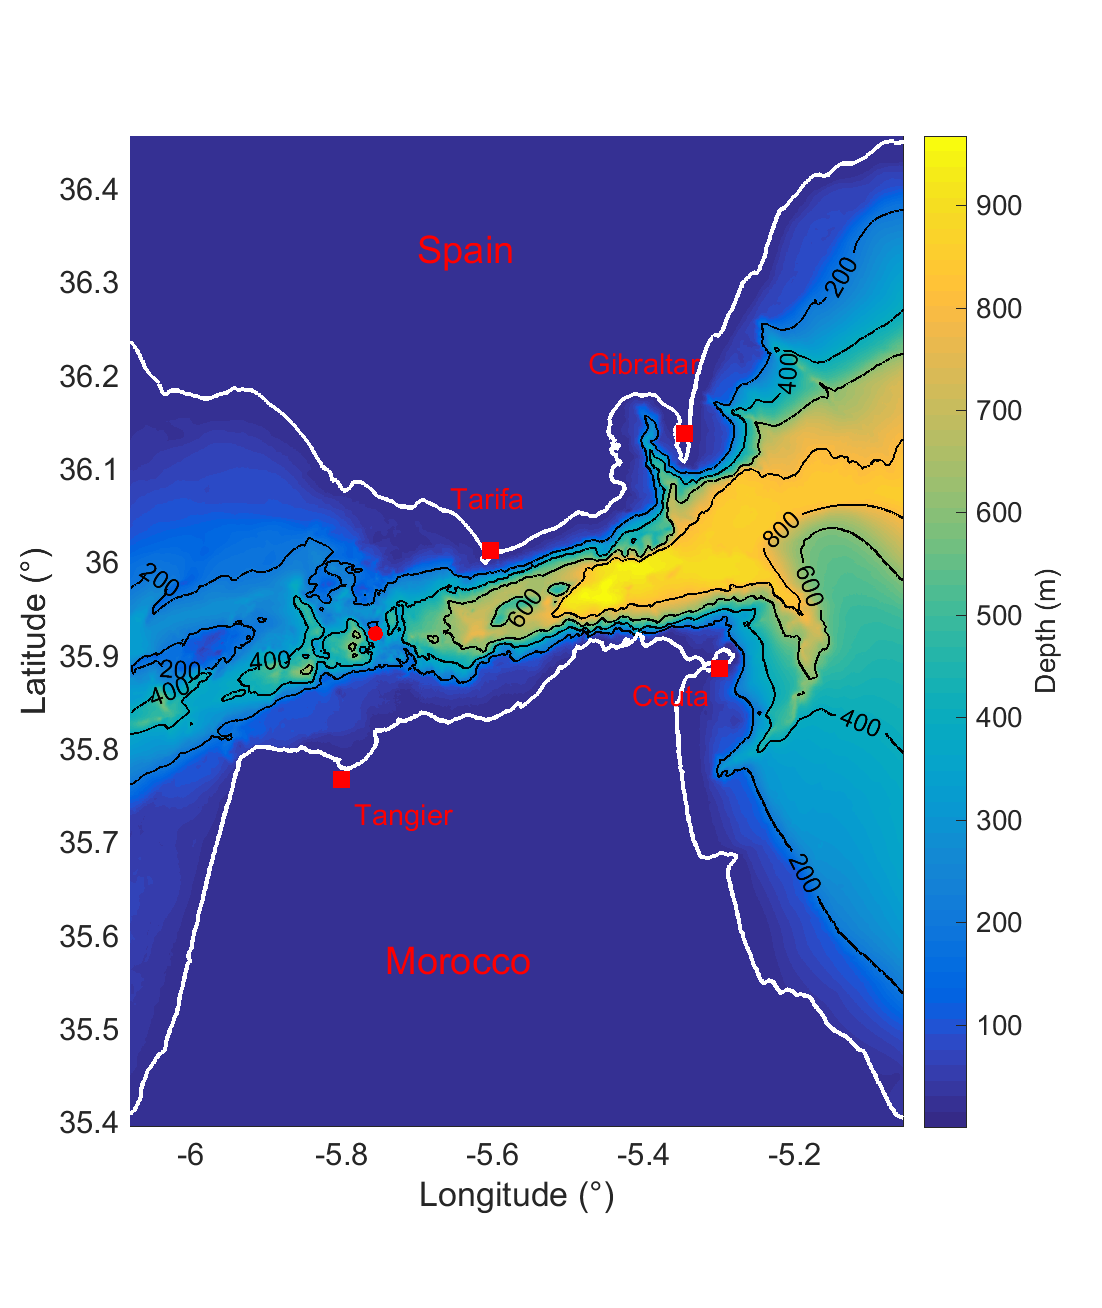
\includegraphics[width=0.5\textwidth]{./GBR3D/FigBathyVHR.png}
        \caption{Area and Bathymetry used for the simulations. The red dot denotes the point at Camarinal Sill where the zonal barotropic current is taken as reference in following figures.!!!Changer en anglais tangIer}
        \label{FigBathy3D}
\end{figure}



\begin{figure}[!h]
        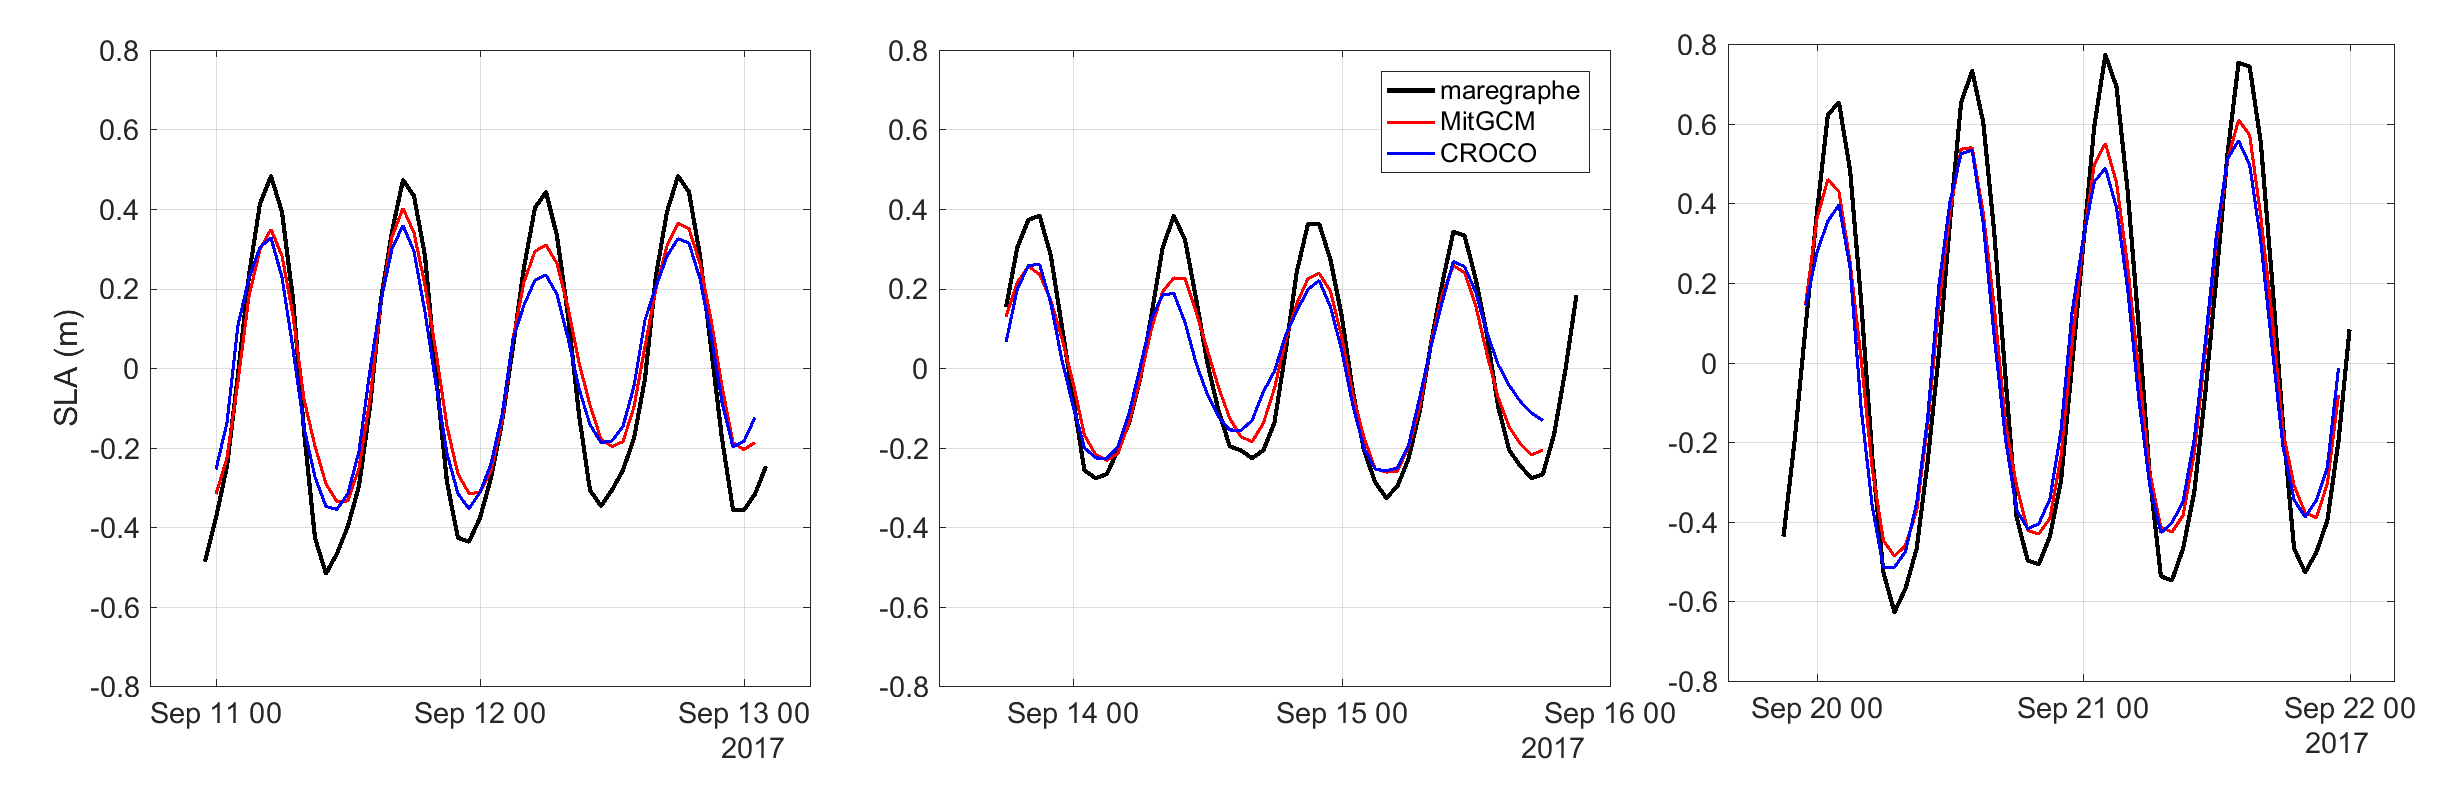
\includegraphics[width=\textwidth]{./GBR3D/SLA_Tarifa_ME2VE2IES.png}
        \caption{Sea level-anomaly at Tarifa from tidal gauge data (black) or at the nearest grid point for parent simulation (red) and CROCO simulation (blue), for situation ME (a), MM (b) et VE (c)}
        \label{fig_maree_tar}
\end{figure}

\subsubsection{Water masses}


\begin{figure}[!h]
        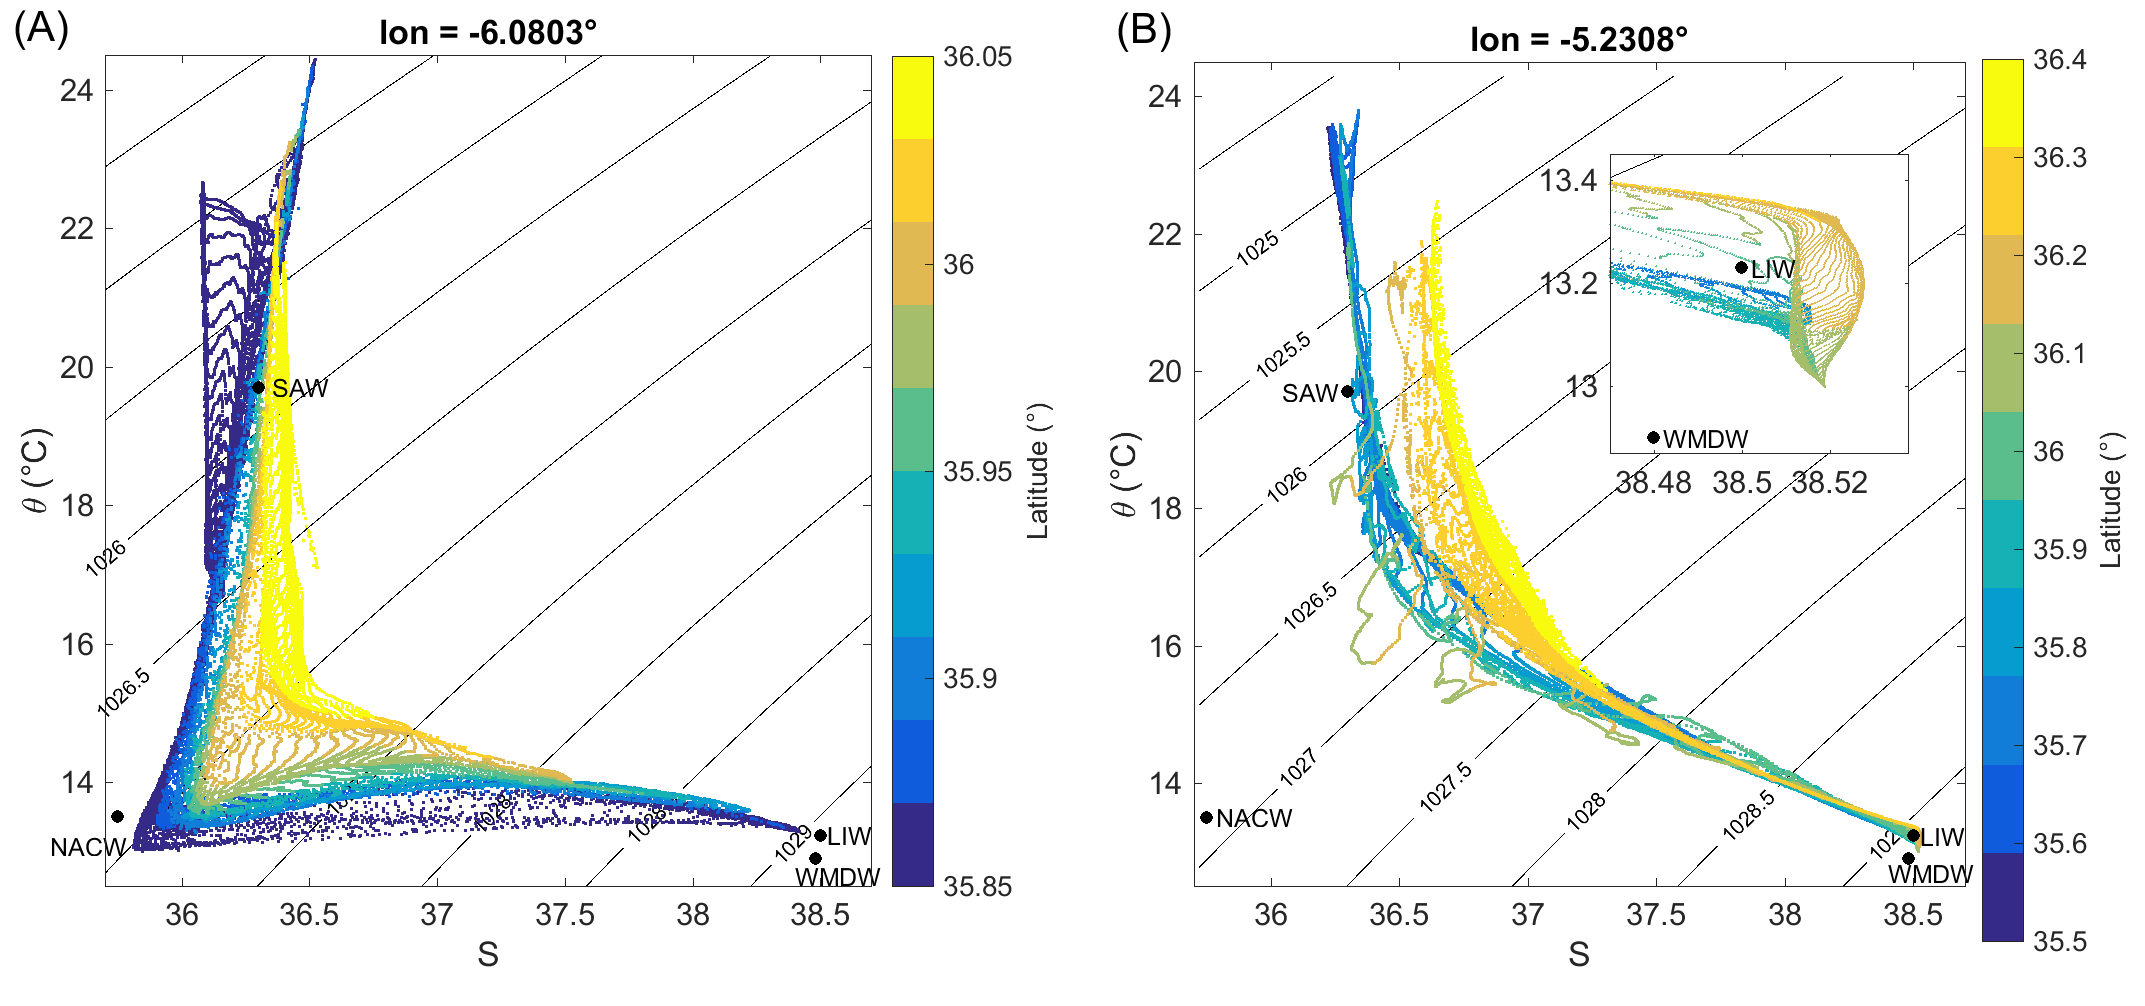
\includegraphics[width=\textwidth]{./GBR3D/WM_ini_IES.png}
        \caption{$\Theta$-S diagrams of grid points at 6.08$^\text{o}$W (a) and 5.23$^\text{o}$W in first timestep of SimIT, color indicates the latitude of each grid point. Are indicated cenroid definition of certain water masses according to Najanro2014}
        \label{Fig_Ini_WM3D}
\end{figure}


Figure \ref{Fig_Ini_WM3D} shows the $\theta$-S diagrams for east and west entry of the Strait in initial tracer field of simulation SimIT. As expected, for med waters see on the west side two signals for the two pathways of the med outflow, on the east side see distinctly a deep water mass and an intermediate one that could be interpreted as analogous to WMDW and LIW, with the latter being present mostly on the northern part, however in the simulation saltier and warmer waters than expected in bibliography. For atl waters, NACW present on west of domain, less on east. On east side, see difference surface water north/south of the opening of the Strait, with saltier surface waters in the north.




\subsection{Numerical diagnosis}
\label{PartDiag3D}

\subsubsection{Interface definition}

The analysis of simulation result is based on two layer definition of an Atlantic waters layer and Mediterranean waters layer. They are defined in regard to a reference salinity, with the interface defined as the height of the first water parcel from the top down in the water column for which salinity is above the reference salinity.

The reference salinity is taken as varying along the Strait as a hyperbolic tangent function of longitude centered at the Camarinal Sill to account for the different water mass composition in the eastern and western part of the Strait of Gibraltar. 

\begin{equation}
	S_i(x)=tanh(\frac{x-X_{CS}}{DX})\frac{S_M-S_m}{2}+\frac{S_M+S_m}{2}
\end{equation}
with $X_{CS}=5.75^o$, $dx=0.25^o$, the location and width of the Camarinal Sill in degrees, $S_M=37.39$ and $S_m=37.1$ the max and minimum values taken respectively east and west of the sill.

%This may not give the perfect interface at any given time...

\subsubsection{Froude layer number}

With the atlantic and mediterranean layers defined as above, the Froude layer number for internal gravity wave is computed at each 2D grid point as : 

\begin{equation}
F_i=\frac{U_i^2}{g'h_i} , \ \text{with} g'=g \frac{\rho_2-\rho_1}{\rho_0}
\end{equation}

where $\rho_i$ averaged density in layer i,  $U$ is averaged velocity norm over the layer i of height h. If $F_i>1$ say that the flow in layer i is supercritical.


\subsubsection{Hydraulic Jump detection, acceleration of flow}

\begin{figure}[!h]
 \centering
 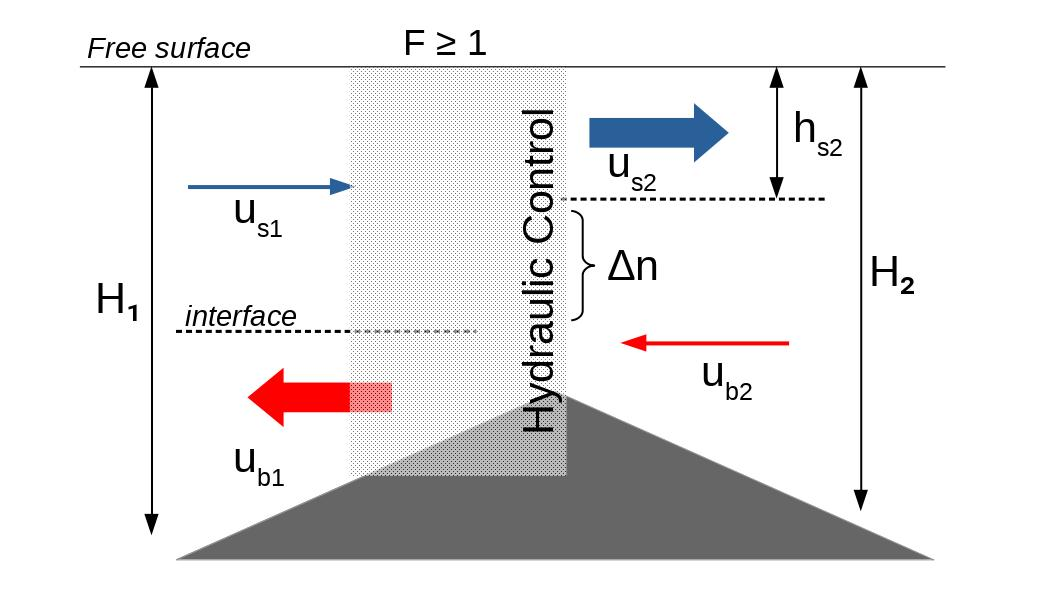
\includegraphics[width=0.5\textwidth]{./GBR3D/schema_diagressaut.jpg}
 \caption {Schematic of flow upstrean and downstream of hydraulic jump at Camarinal Sill, Strait of Gibraltar}
  \label{schemaRH}
\end{figure}


A simple diagnosis for detection of the hydraulic jump at Camarinal Sill in the simulations is based on the impact such a structure has on the flow. As shown/schematized/sketched(?) in figure \ref{schemaRH}, hydraulic jump (also called hydraulic drop) induces a drop of the interface depth. Since the flow in the Strait is canalised by bathymetry (for med flow) and coast (for atl flow), there must be conservation of flux from one section downflow and upflow of the hydraulic jump, which with the variation of the interface depth, means acceleration/deceleration of flow (depending on which layer is reference).

The drop in interface depth is noted $\Delta n=b_2-b_1$, the variation of bottom depth $\Delta H=H_2-H_1$ and the acceleration in the bottom layer $\Delta u_b = u_2-u_1$. For the bottom layer conservation of flux is :
\begin{subequations}
\begin{alignat}{2}
  \displaystyle
&u_1 (H_1-b_1)&& = u_2 (H_2-b_2)\\
& &&= u_1 (\Delta H + \Delta n) + u_1 (H_1-b_1) + \Delta u_b (H_2-b_2)
\end{alignat}
\end{subequations}

\begin{equation}
\Delta u_b = -u_1 \frac{\Delta H + \Delta n}{H_2-b_2}
\end{equation}

For the surface flow, similarly can find
\begin{equation}
\Delta u_s = - u_1\frac{\Delta n}{b_2}
\end{equation}

Velocity in the area of the hydraulic jump must validate condition of (at least) critical flow, ie Froude number $\geq$ 1. We search minimal condition for hydraulic jump so $F=1$, or $U=c$, taht is the flow ceerity equals the phase speed of internal wave. If for the latter we take the definition of interfacial speed can have an expression for $u_1$: 
\begin{equation}
|u_1|=c=\sqrt{g' \frac{(H_1-\Delta n - b_2)(\Delta n + b_2)}{H_1}}
\end{equation}



In the end, some parameters are chosen as threshold, here take values that should be correct for area of camarinal sill, the minimum excursion of the jump $\Delta n = 30m$ and the height of the Atl layer $b_2=50 m$ , and the reduced gravity $g'=0.02 m s^{-2}$.

\subsubsection{Q parameter and derivated diagnosis}

We want to detect primary shear instabilities in the Med outflow. A simple vorticity diagnosis is not chosen as it requires choosing the rotation axis, but also because regions of high shear such as between the MEd outflow and Atl waters will have high vorticity values. Instead, analogously to the use of the Okubo-Weiss parameter in Hilt 2020, we chose to compute parameter Q, defined as (ref):

\begin{equation}
Q=-\frac{1}{2} \frac{\partial u_i}{\partial x_j} \frac{\partial u_j}{\partial x_i} = \frac{1}{2} (\Omega_{ij}\Omega_{ij} - S_{ij} S_{ij})
\end{equation}
with $u_i$ the components of velocity vector, and $S_{ij}$ and $\Omega_{ij}$ are respectively the strain-rate tensor and vorticity tensor. When $Q>0$, rotation is predominant over shear part.


Due to advection by the Med outflow, a succession of primary instabilities will propagate over teh same grid cells. The temporal evolution of Q over such grid cell will show oscillations between high positive value (center of a billow/vortex) and low negative values (shear between two consecutive billows). A proxy to detect this area is chosen as high value of standard deviation of parameter Q, as defined in equation \ref{eqstdQ} where the over bar denotes temporal average over 30 minutes, a period over which there will be minimal modification of the general flow in the Strait.

\begin{equation} 
\label{eqstdQ} 
    std ( Q ) (\vec{x},t)=  \sqrt{   \overline{Q (\vec{x},t)^{2}} -  \overline{Q(\vec{x},t)}^{2}  }
\end{equation}

To create 2D maps presented in next section, only the maximal value of standard deviation in the water column is saved...
By implementing this calculation directly in the code, we can asses where instabilities/vortexes propagate without having to make a huge volume of simulation outputs over the whole domain, those economising in storage place and data readability. 

The result of this proxy can be compared to the result of the Singular Value Decomposition (SVD) of the time-varying 3D field. However this calculation is off-line and necessitates a high frequency 3D output to pick up the relevant structures.



\subsection{Results}
\label{section3DRes}

\subsubsection{Flow criticality/Hydraulically controlled layer and hydraulic jump, neap-spring tide variability}


\begin{figure}[!h]
 \centering
 
 \begin{subfigure}{\linewidth}
\centering
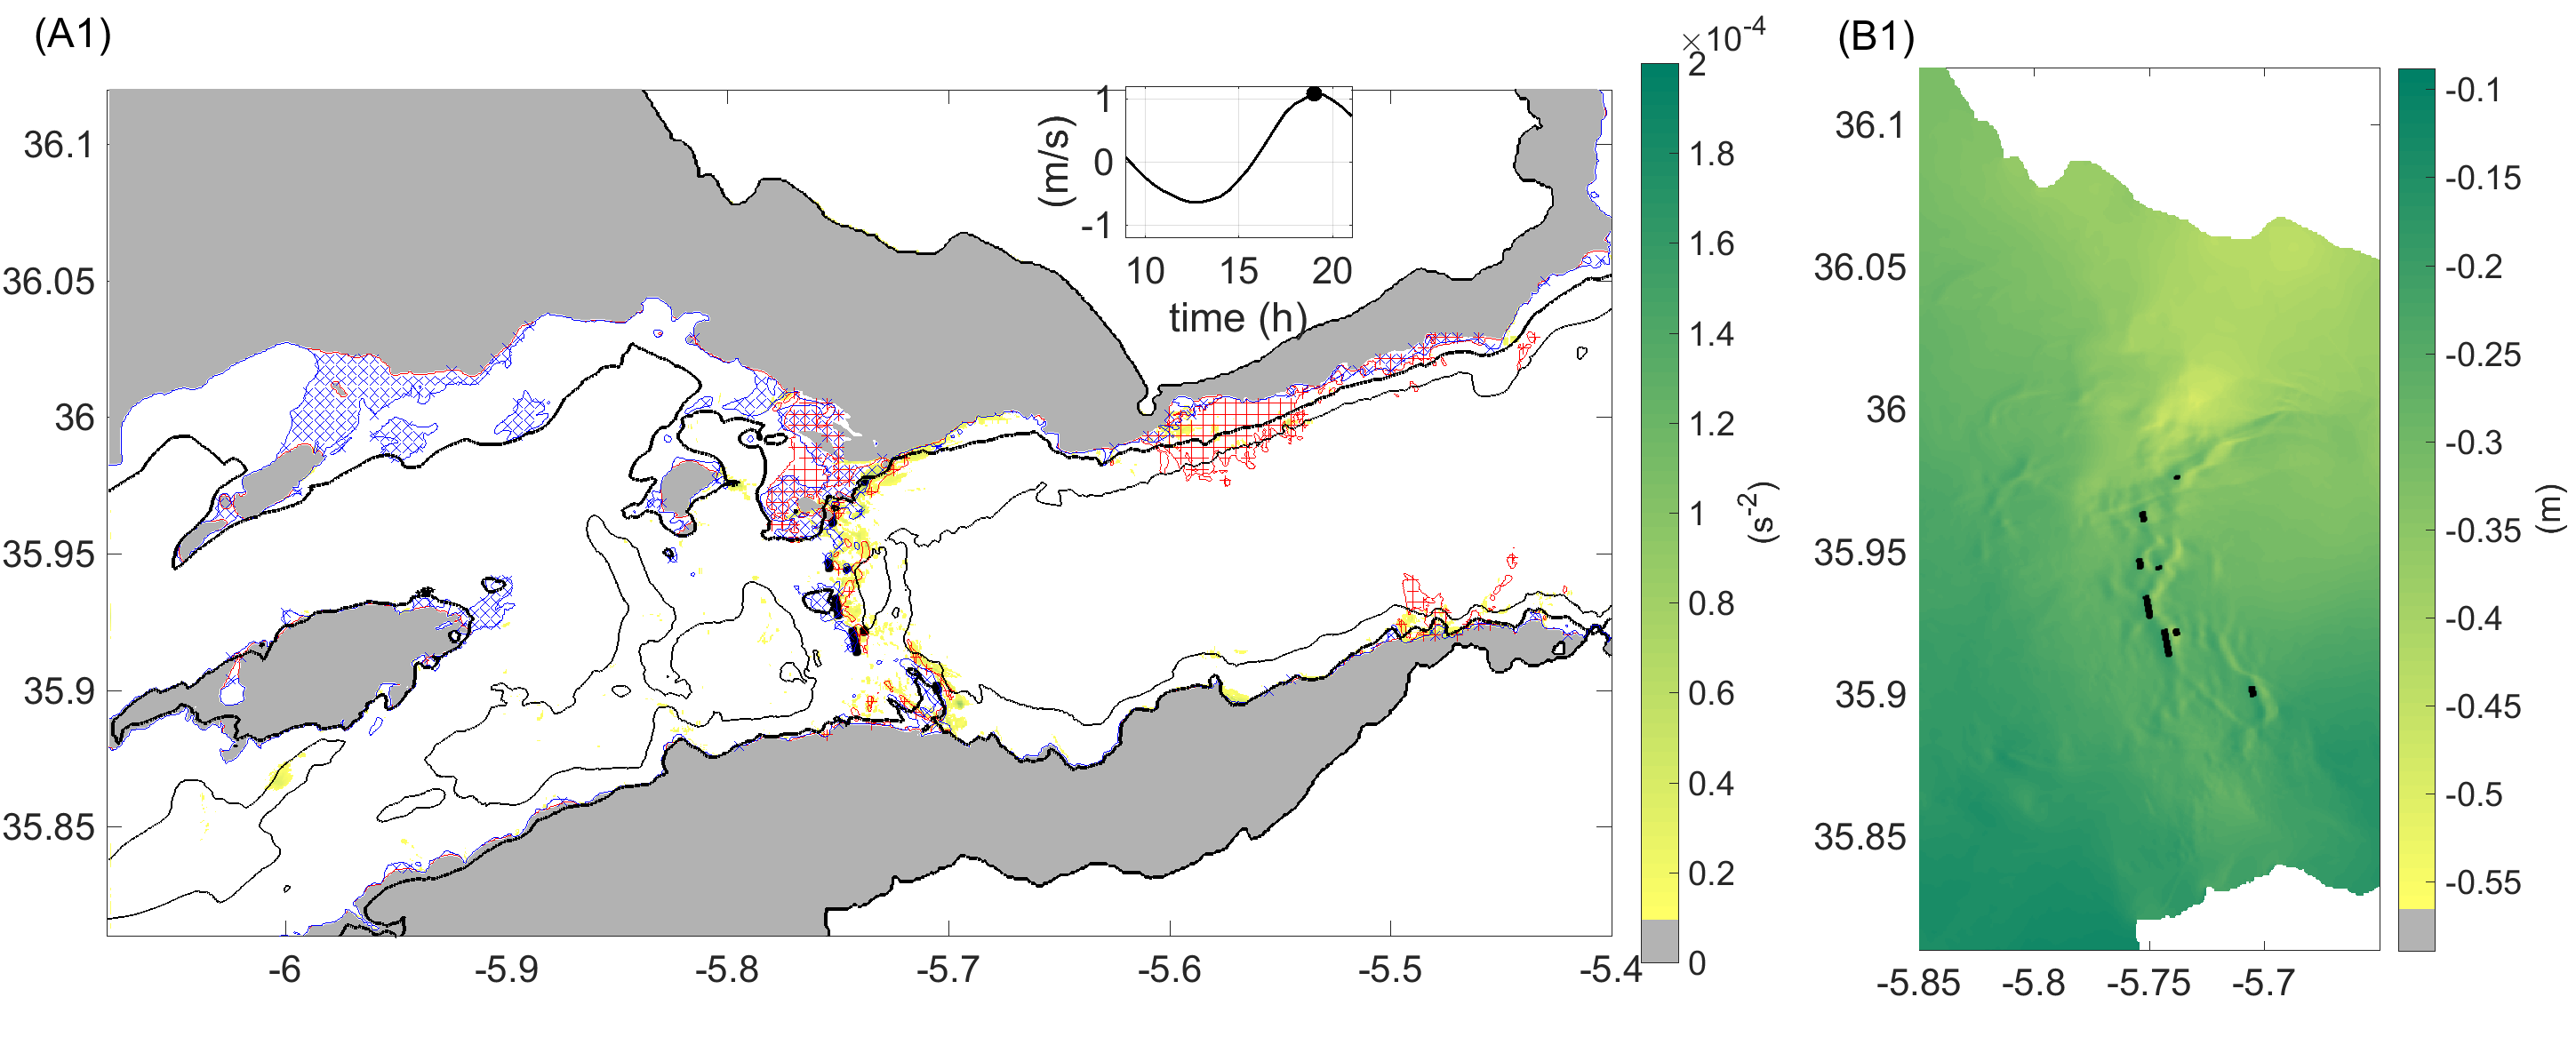
\includegraphics[width=1\linewidth]{./GBR3D/ME2_19h_p.png}
\end{subfigure}
 
 \begin{subfigure}{\linewidth}
\centering
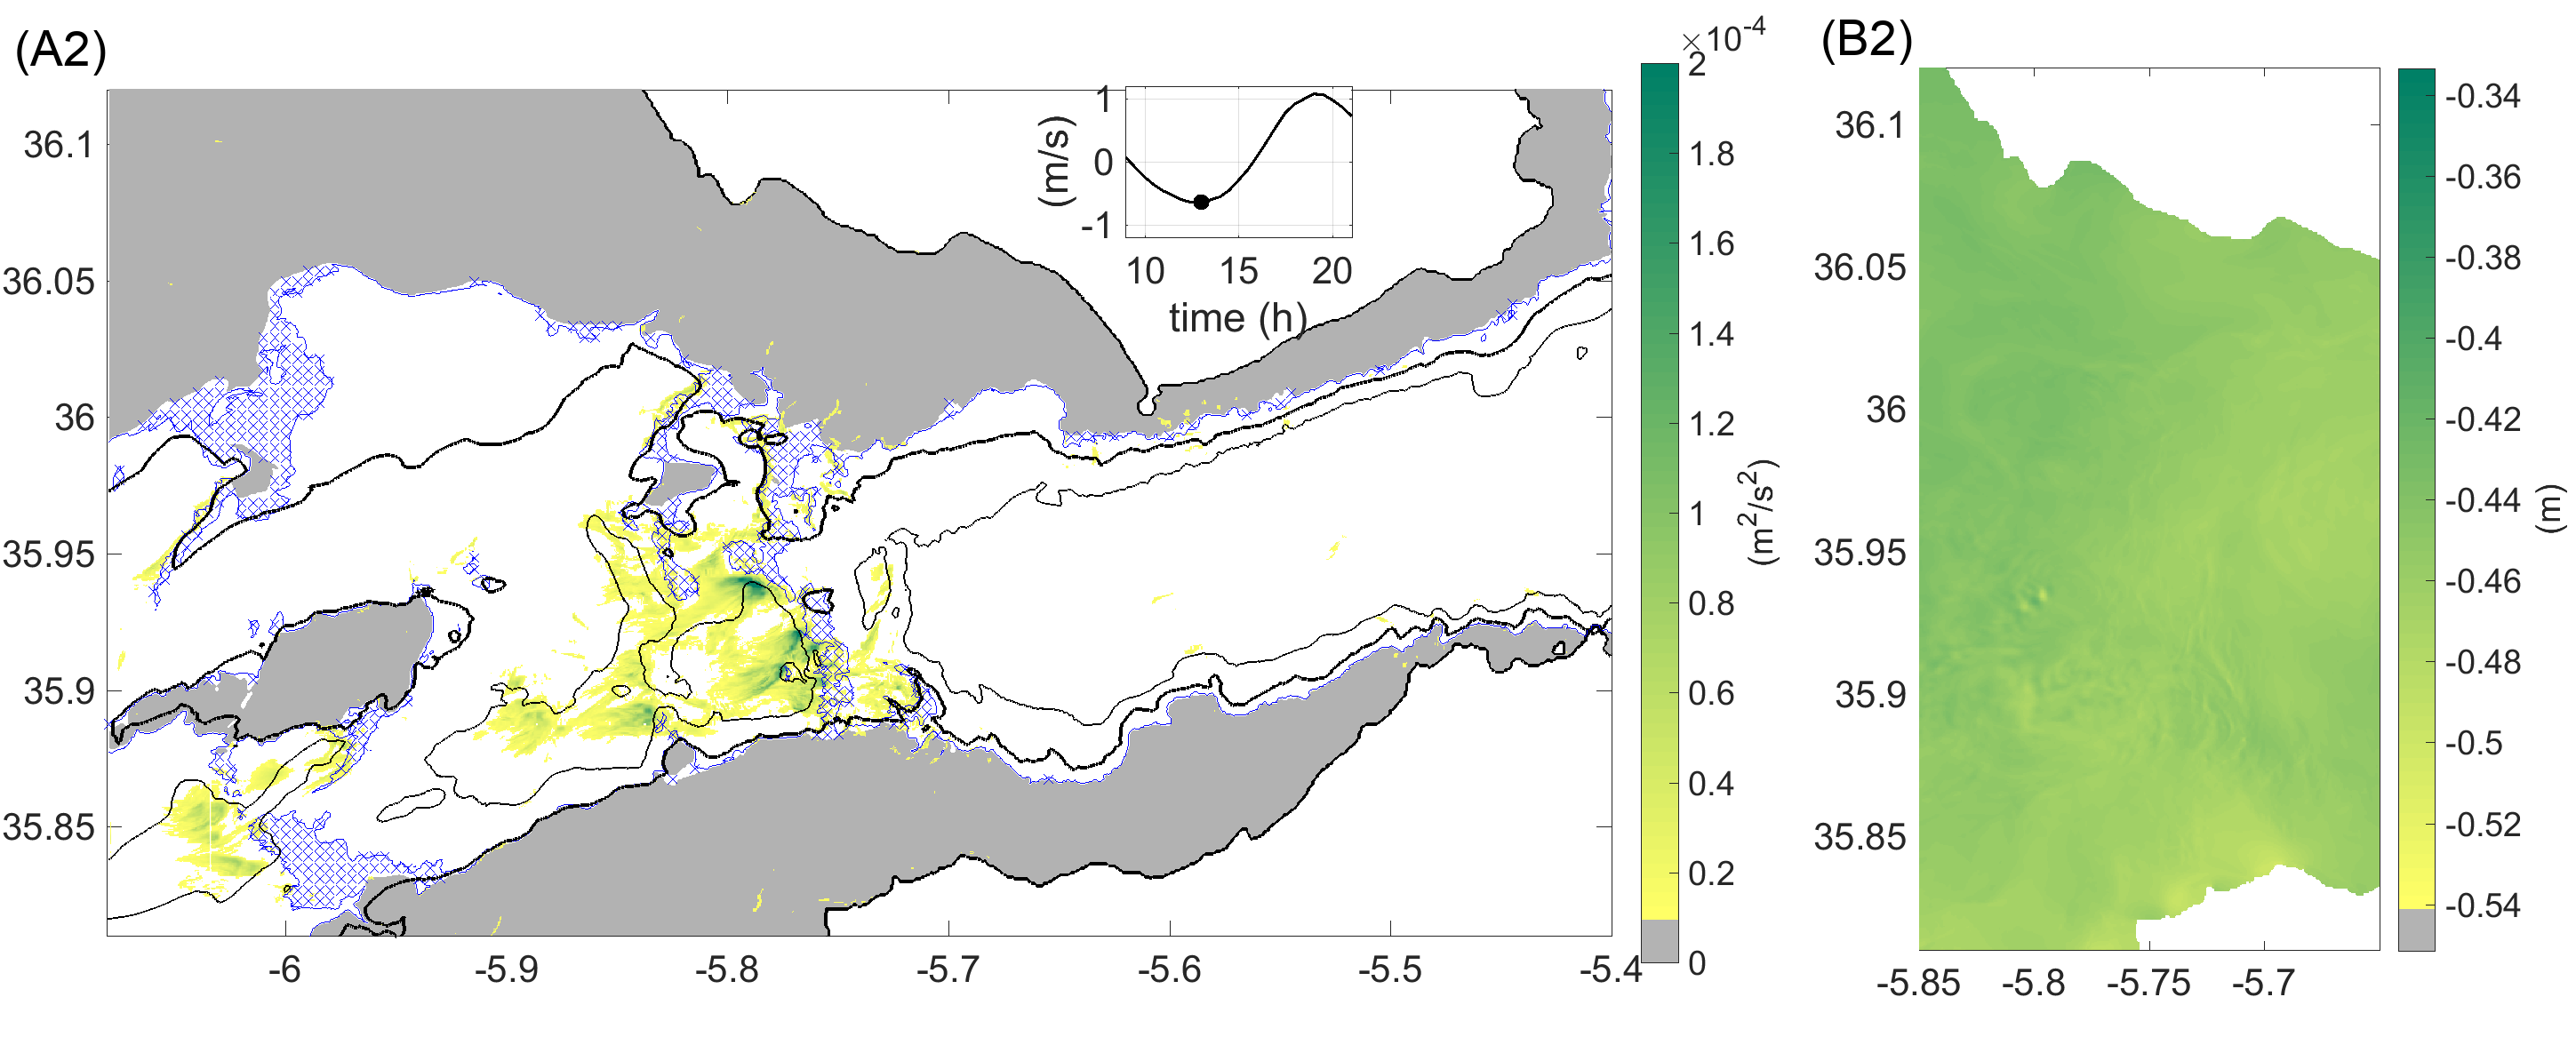
\includegraphics[width=\linewidth]{./GBR3D/ME2_13h_p.png}
\end{subfigure}
\caption {For simulation SimNT, an inflow then an outflow of type \textit{no-jump}. Blue (red) shaded area is supercritical med (atl) layer. Black dots are hyd jump detection. grey area denotes where S bottom$<$Sinterface. colorbar for standard deviation of parameter Q (only values above $10^-5$are represented). Also inicated barotropic znal current at CS (point indicated in figure \ref{FigBathy3D}). Two black isobathes contours are indicated, 200m (bold) and 400m(thin) depth  }
\label{FigHCN}
\end{figure}

Figures \ref{FigHCN} to \ref{FigHCI} present several diagnosis for series of maximal outflows and inflows for variable strength of the tidal forcing among simulations SimNT,SimST then SimIT. Are represented the diagnosis presented in paragraph \ref{PartDiag3D} : the area of supercritical flow in atl and med layer as shaded areas, the detection of hydraulic jump, and area of standard deviation of parameter Q, which indicate were vortices are propagating. The grey area indicates where the salinity in the bottom level is below the interfacial salinity as defined in paragraph ..., and thus were it is considered only Atlantic waters circulate.

Figure \ref{FigHCN} presents a situation of weak barotropic currents ($<1m/s$ at a shallow point of Camarinal Sill) in outflow and inflow and is considered a 'neap-tide' case, figure \ref{FigHCS} is for strong barotropic currents ($\geq 1.5m/s$) for the in- and outflow of a 'spring-tide' case. Finally, figure \ref{FigHCI} is the case of an outflow for an intermediate strength ($\approx 1m/s$)of the barotropic currents.

\begin{figure}[!h]
 \centering
\begin{subfigure}{\linewidth}
\centering
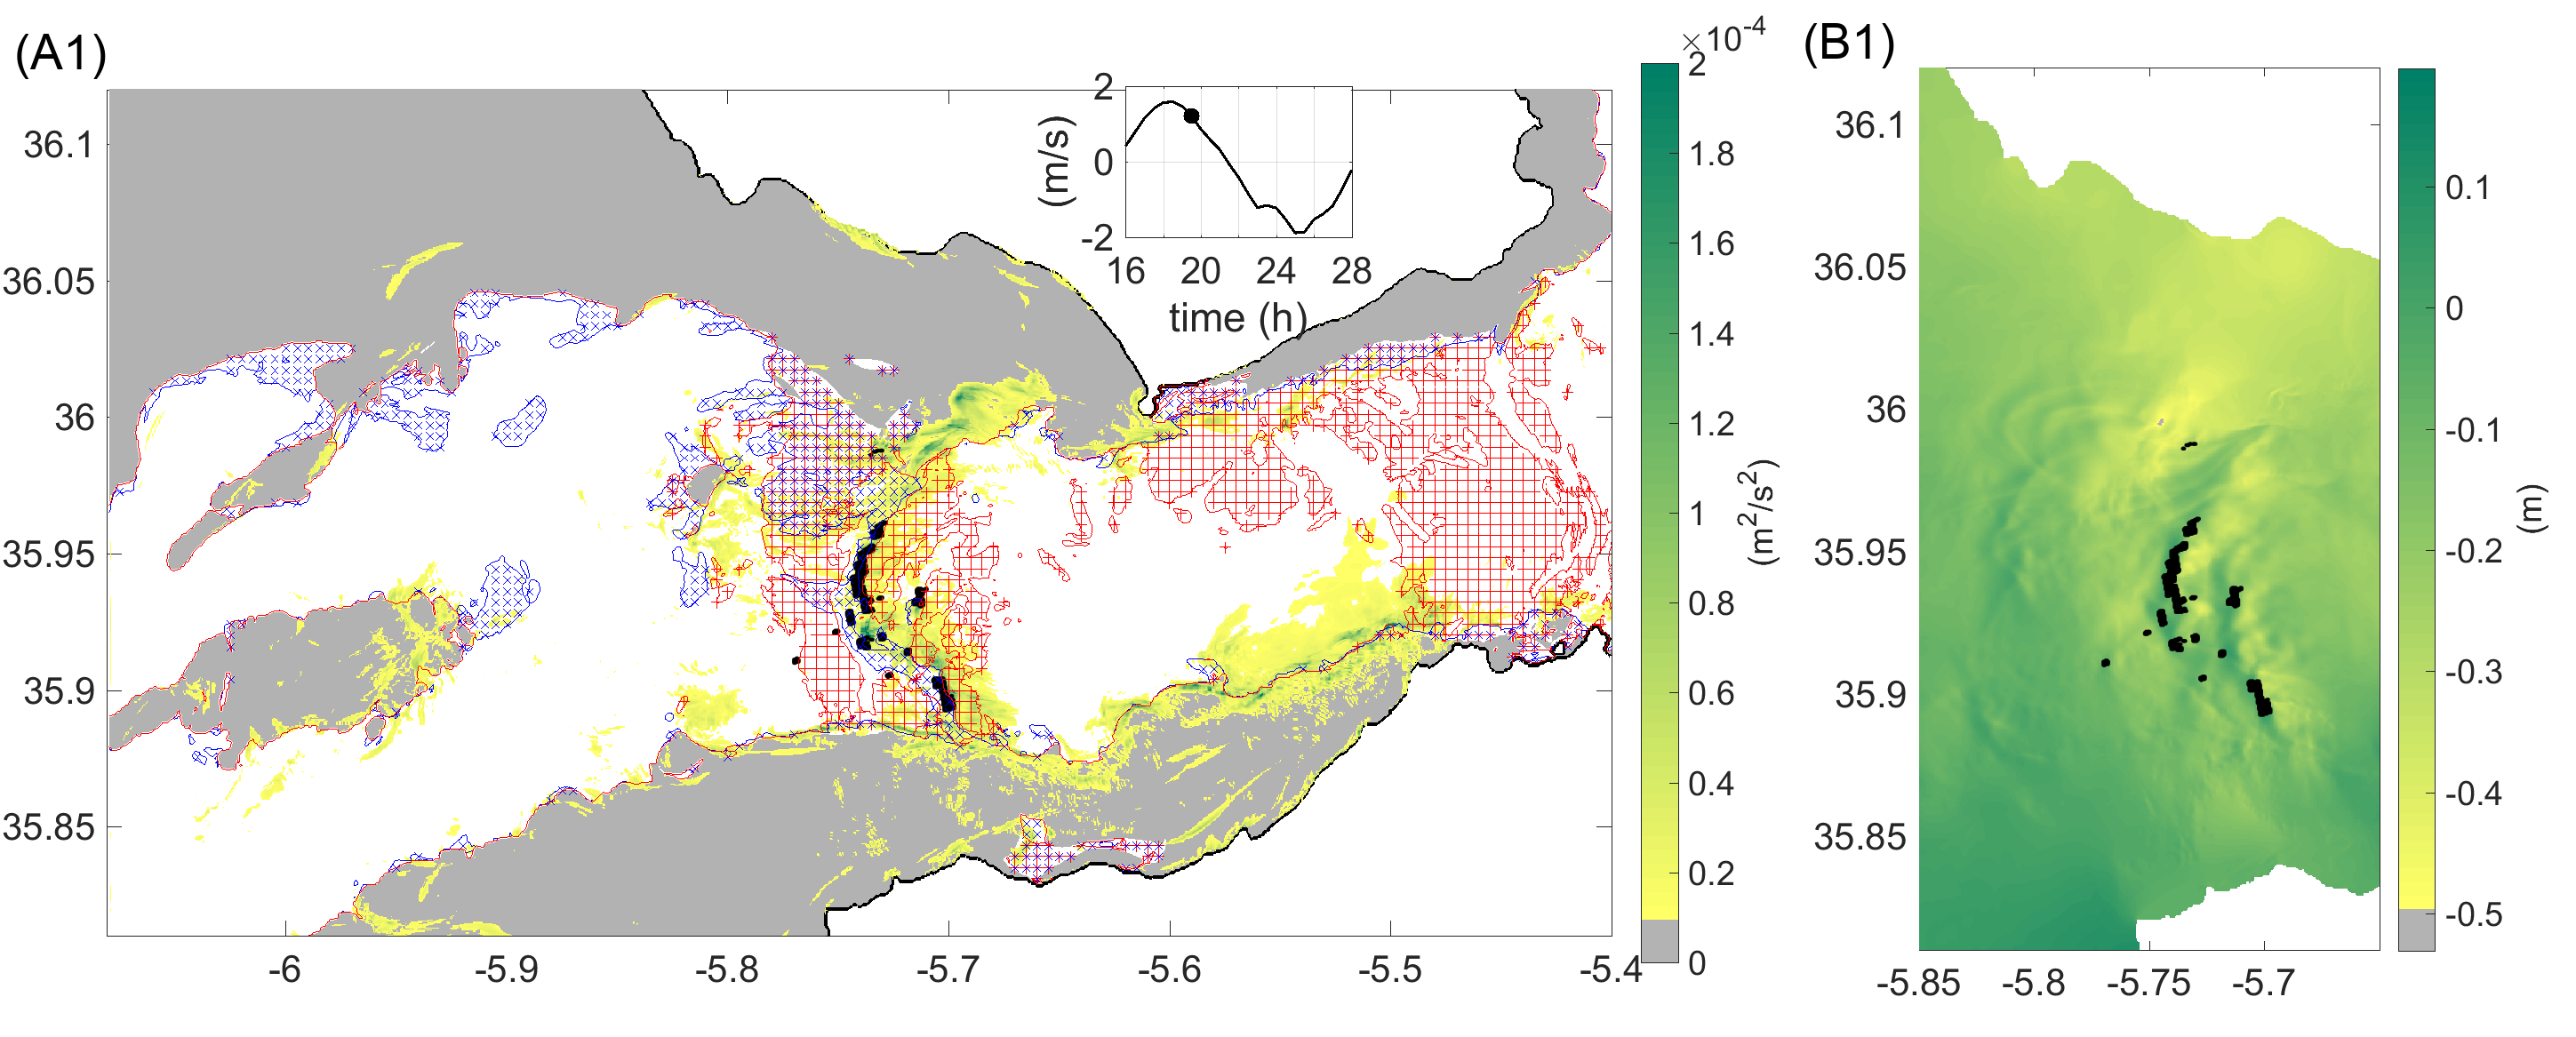
\includegraphics[width=\linewidth]{./GBR3D/VE2_19h30_p.png}
\end{subfigure}

\begin{subfigure}{\linewidth}
\centering
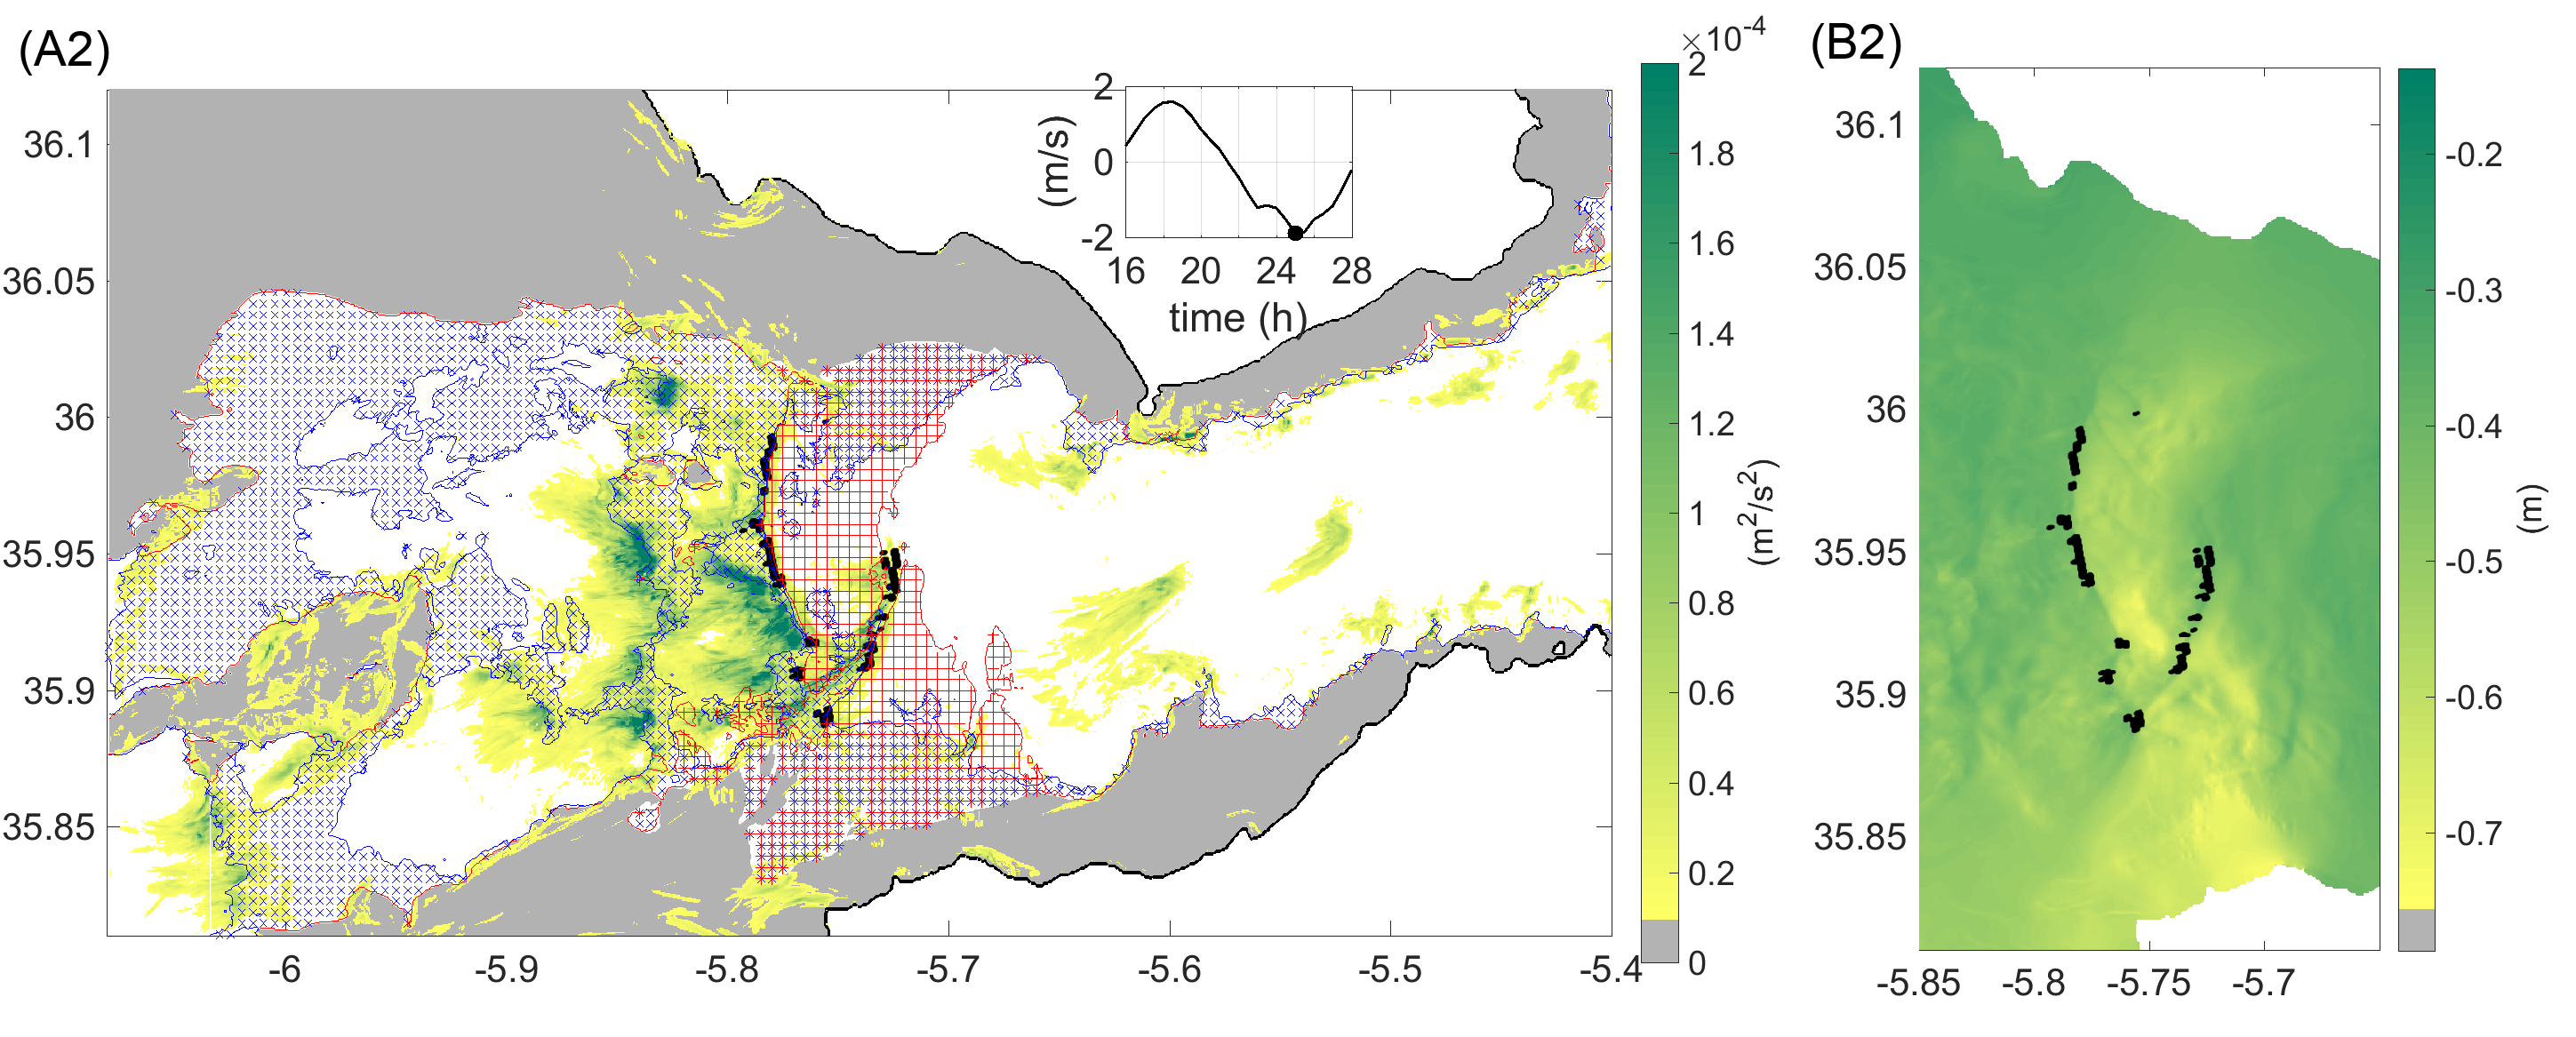
\includegraphics[width=\linewidth]{./GBR3D/VE2_25h_p.png}
\end{subfigure}
\caption {Same as figure \ref{FigHCN} for simulation SimST in inflow and outflow of type \textit{w-jump}}
\label{FigHCS}
\end{figure}

\begin{figure}[!h]
 \centering
%\begin{subfigure}{\linewidth}
%\centering
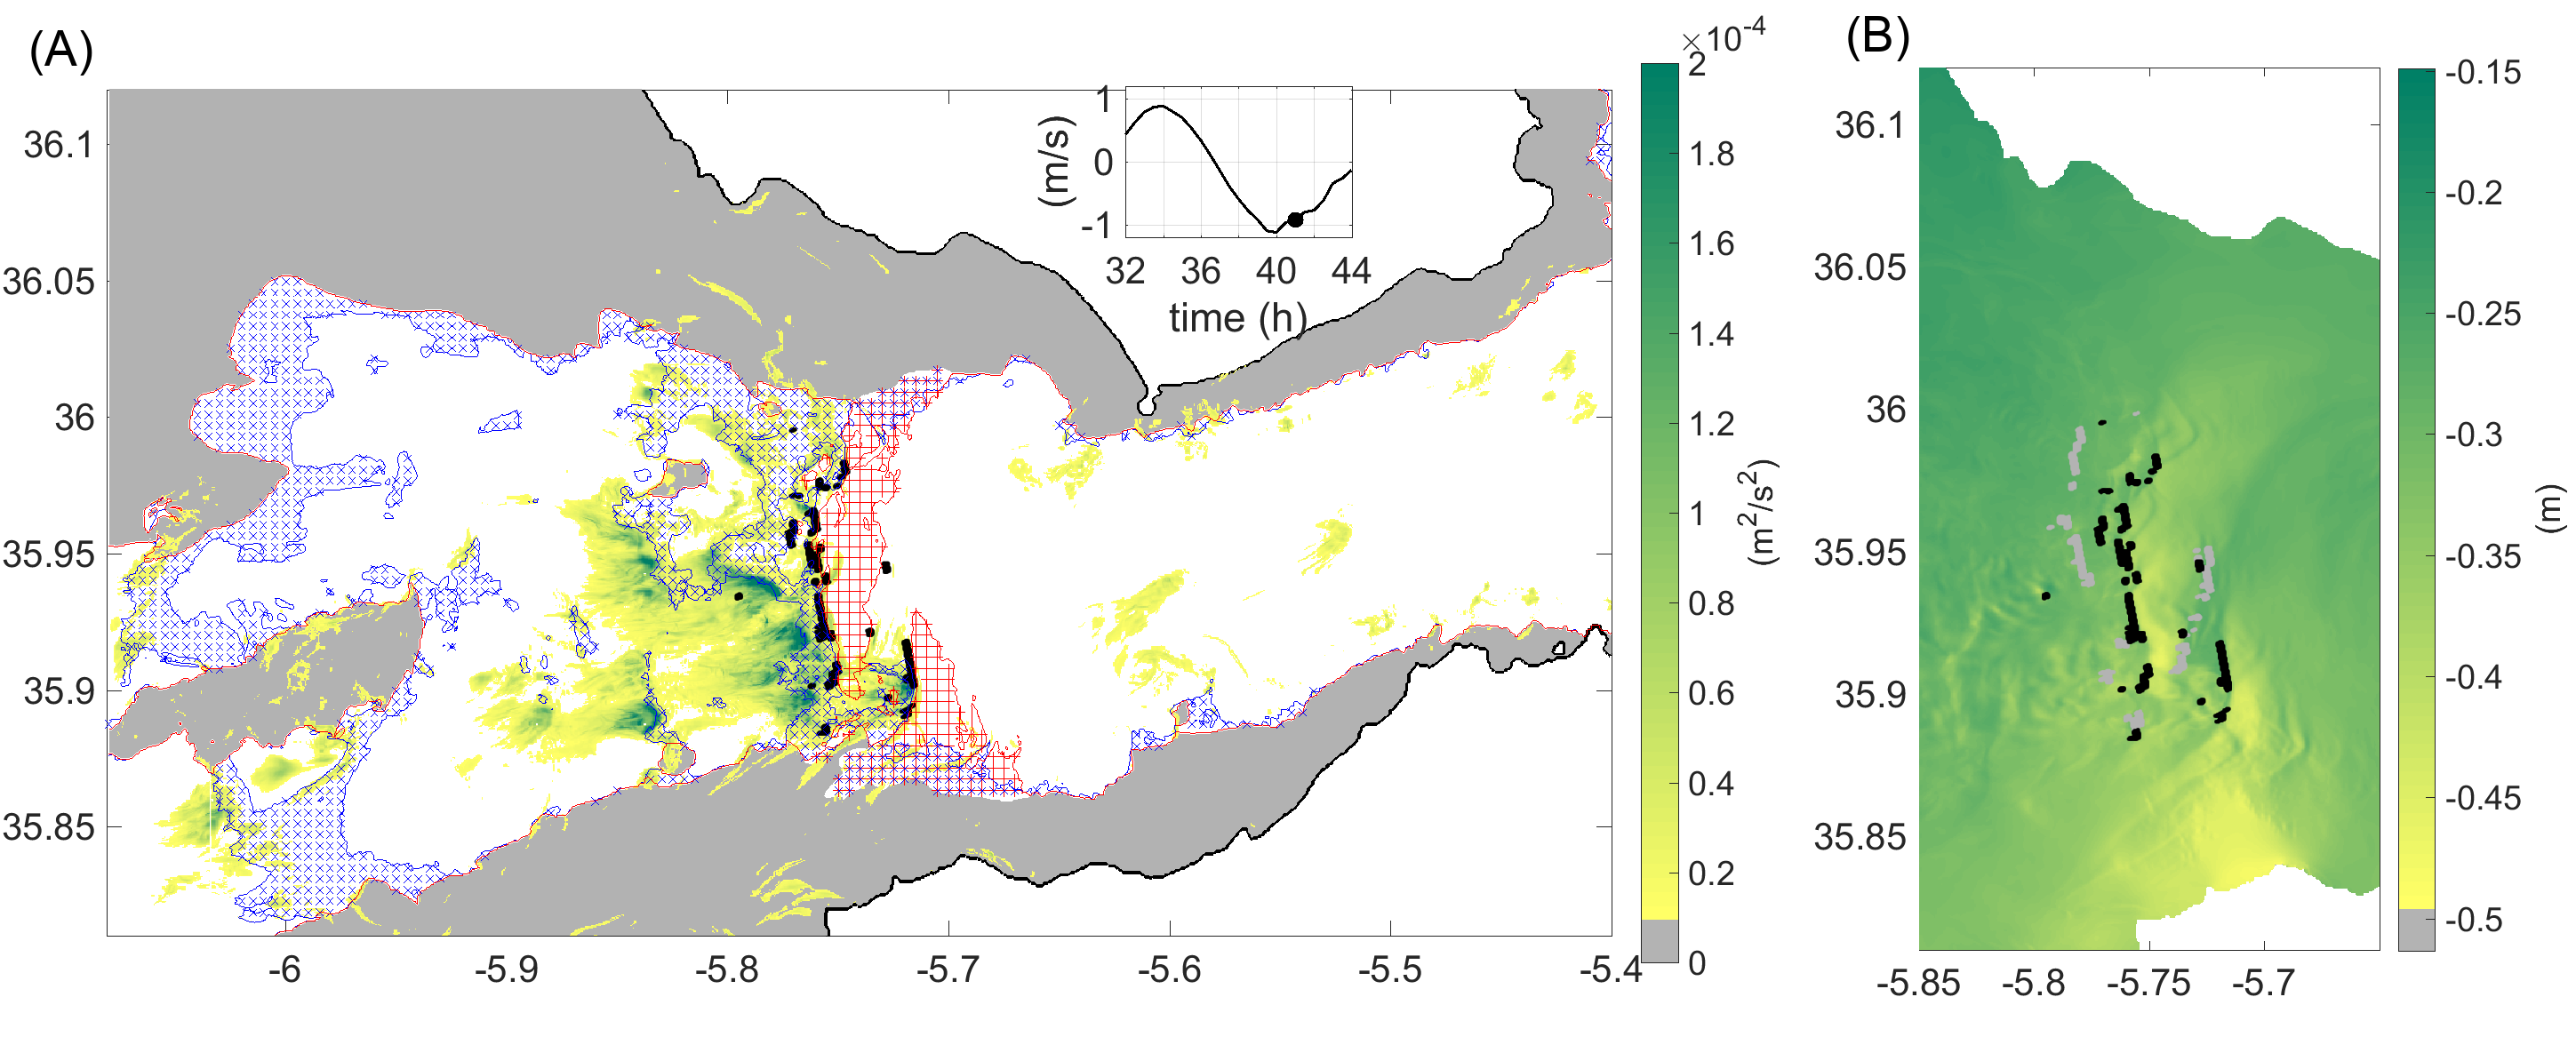
\includegraphics[width=\linewidth]{./GBR3D/IES_41h_p.png}
%\end{subfigure}
 \caption {Same as figure  \ref{FigHCN} for simulation SimIT and an outflow of type {s-jump}, on figure SLA also put trace of jump of spring tide outflow}
 \label{FigHCI}
\end{figure}

Firstly, can see two channels west of the Camarinal Sill where Med layer is present, separated by Majuan Bank. The path of the med vein through the south channel does not change much, however in the northern channel see a variable area of circulation for med waters above 200m depth and centered at 36$^\text{o}$ N. This area is larger during outflows, as med waters are driven up-slope by the westward barotropic current, but there is also a southern component to the flow that bends back into the main north channel (see figure \ref{FigBathy3D} for a better view of the bathymetry of the area).

For all cases, supercriticality of the atlantic (mediterranean) layer happens mostly east (west) of 5.8$^\text{o}$W which is the western slope of Camarinal sill. During inflows in figure \ref{FigHCN}.a and \ref{FigHCS}.a, criticality of the mediterranean layer only occurs in patches, the most extended one in the area of the northern channel discussed above. In outflows in figures \ref{FigHCN}.b,\ref{FigHCS}.b and \ref{FigHCI} the Mediterranean layer is supercritical at both Camarinal, Espartel Sill and northern channel for all cases. In the spring tide outflow case especially, most of the northern channel has a supercritical flow while at Espartel there is not much difference between the intermediate and spring tide outflow cases.


During outflow supercritical atl layer only at CS, except in neap case where it does not occur at all. In the case where both layers are supercritical at CS, hydraulic jump is detected. It is located at the junction between an area where atl and med layer are supercritical. It follows area of high gradient of free surface elevation.  Find accross all simulated tidal cycle three type of flow at Camarinal Sill during outflow : no hydraulic jump as in figure \ref{FigHCN}.b (\textit{no-jump}), a hydraulic jump situated just above the sill (figure \ref{FigHCI}, \textit{s-jump}), and a hydraulic jump situated over the west slope of the Camarinal Sill (figure \ref{FigHCS}.b, \textit{w-jump}). In this latter case, the hydraulic jump actually starts forming over the sill's crest as in the s-jump case but as the tidal currents strengthen, the area of supercritical atl layer area develops westward and so does the junction where can observe the jump.

Also see hydraulic jump during inflows, located in the same area over the east slope of CS regardless of the strength of tidal currents, but more pronounced with stronger barotropic currents, associated with transition of flow upstream of area of supercritical atl layer.

East of Camarinal Sill, another area of supercritical Atl layer appears during inflows. In neap-tide case, as a patch near north shore in TN at 5.59$^o$W. for spring tide case, this patch is more extended, and a secondary area of supercritical atl flow exists between 5.5$^o$W and 5.4$^o$W, extending from the north to the south side of TN. 

Figure \ref{FigISWGBR3D} shows the field of surface current divergence in Tarifa Narrows while a train of ISW is propagating, figure a for condition of intermediate strength of barotropic current in inflow and figure b for a strong barotropic current at the same time as figure \ref{FigHCS}.b. Are also shown the areas of critical atlantic layer flow as black meshed area. The propagation of the ISW train occurs at the same time as maximum inflow in this area and see the area of atl layer criticality is west of the propagating wave train . It seems the northern part of the criticality of the atl layer is dissociated from its southern part. The former occurs most often and is more or less extended while the other may be affected by influence of the passage of the ISW, either due to induced velocity or change of stratification.



\begin{figure}[!h]
 \centering
%\begin{subfigure}{\linewidth}
%\centering
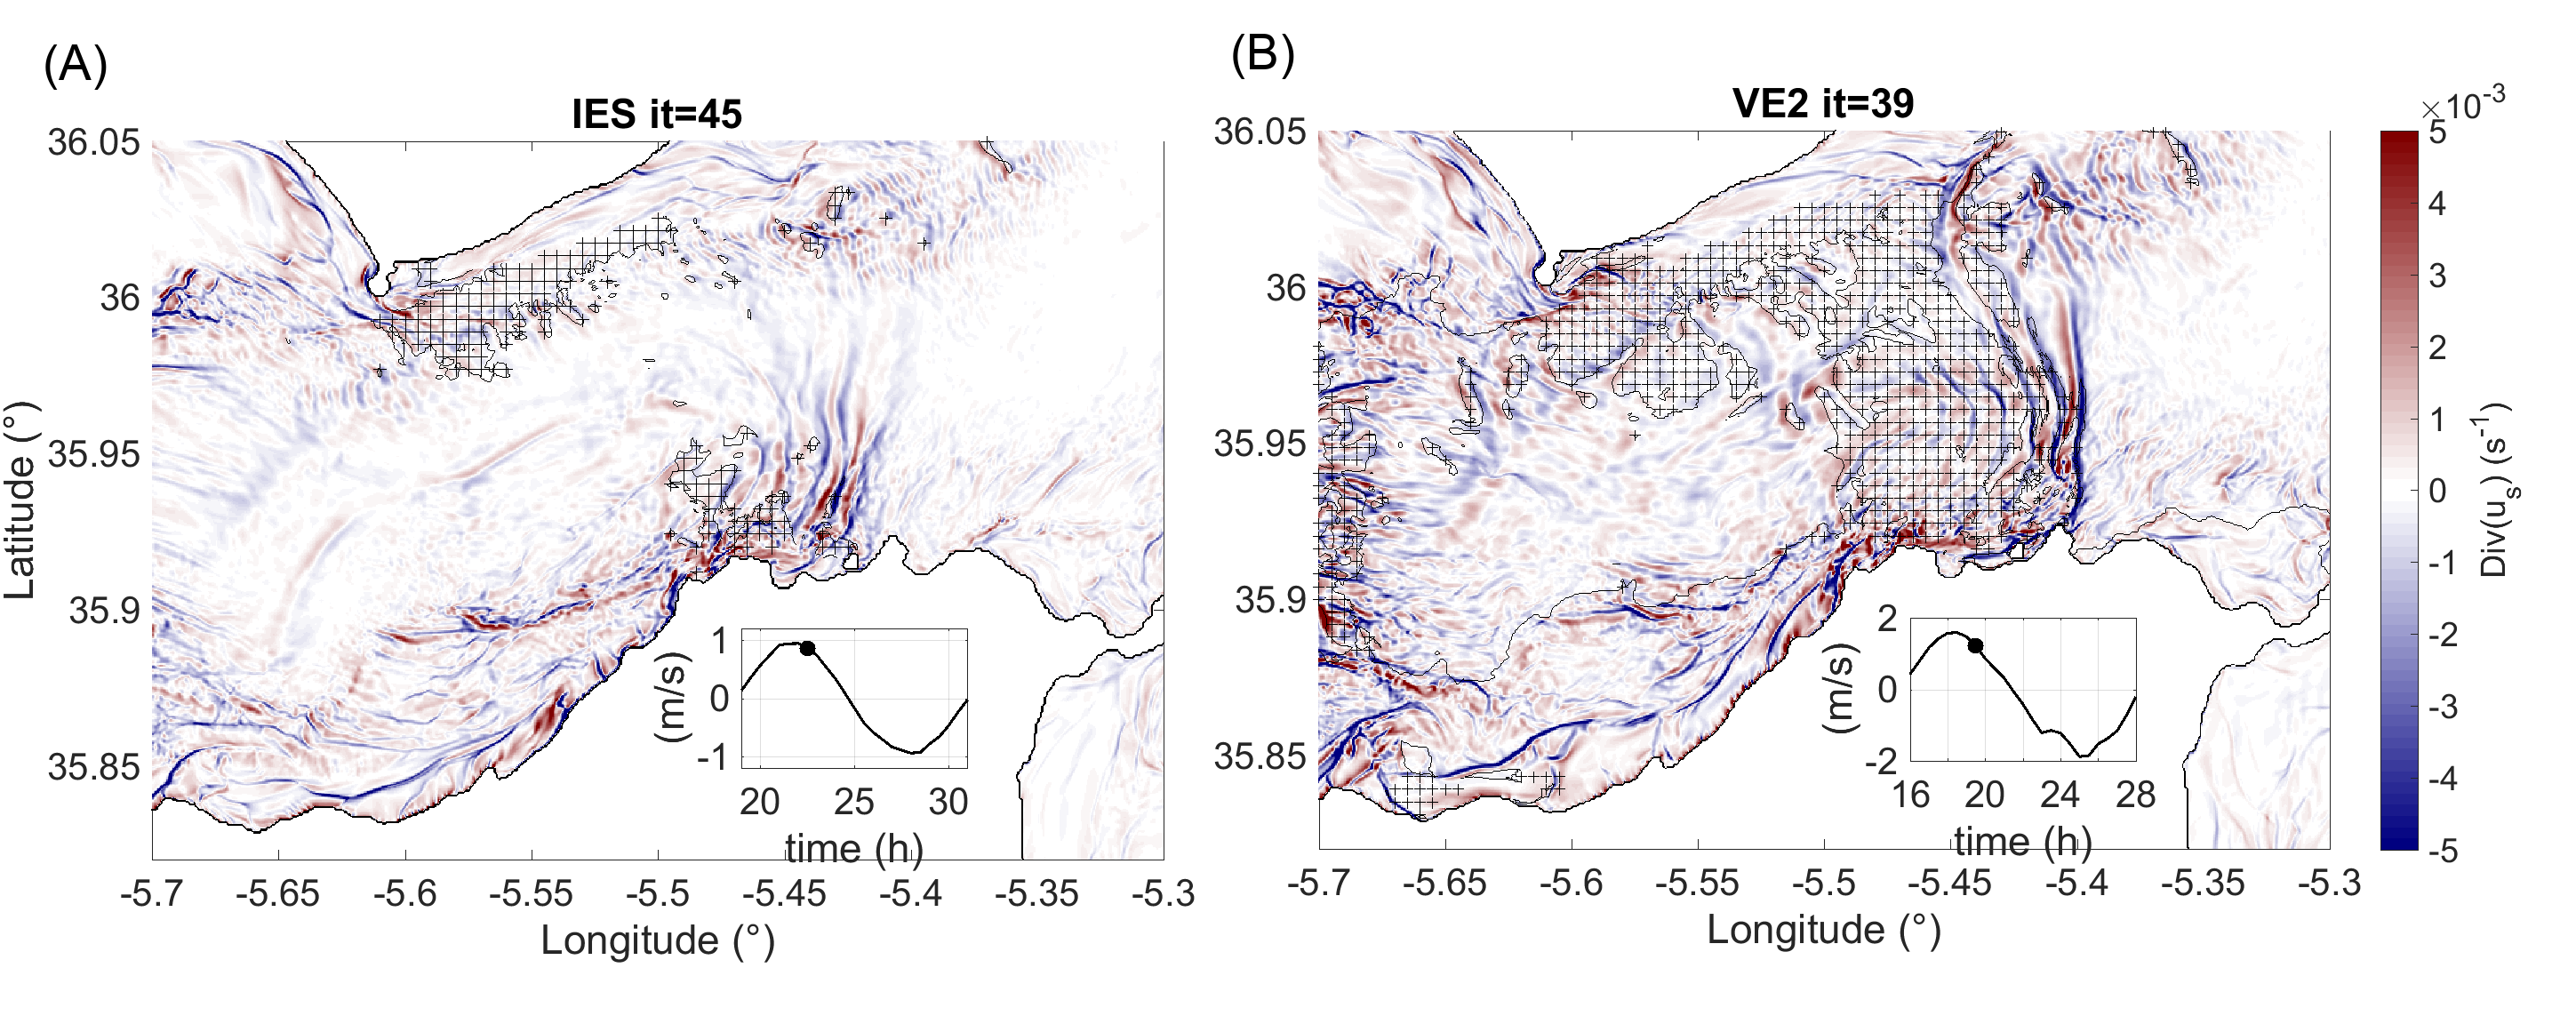
\includegraphics[width=\linewidth]{./GBR3D/FigWaveCont.png}
%\end{subfigure}
 \caption {Divergence of surface current (color) and area of supercritical atlantic layer (black hatchs) at t=22.5H in SimIT (a) and t=19.5H in SimST (b)}
 \label{FigISWGBR3D}
\end{figure}


\subsubsection{Propagation of Solitons (ISWs)}



\begin{figure}[!h]
 \centering
 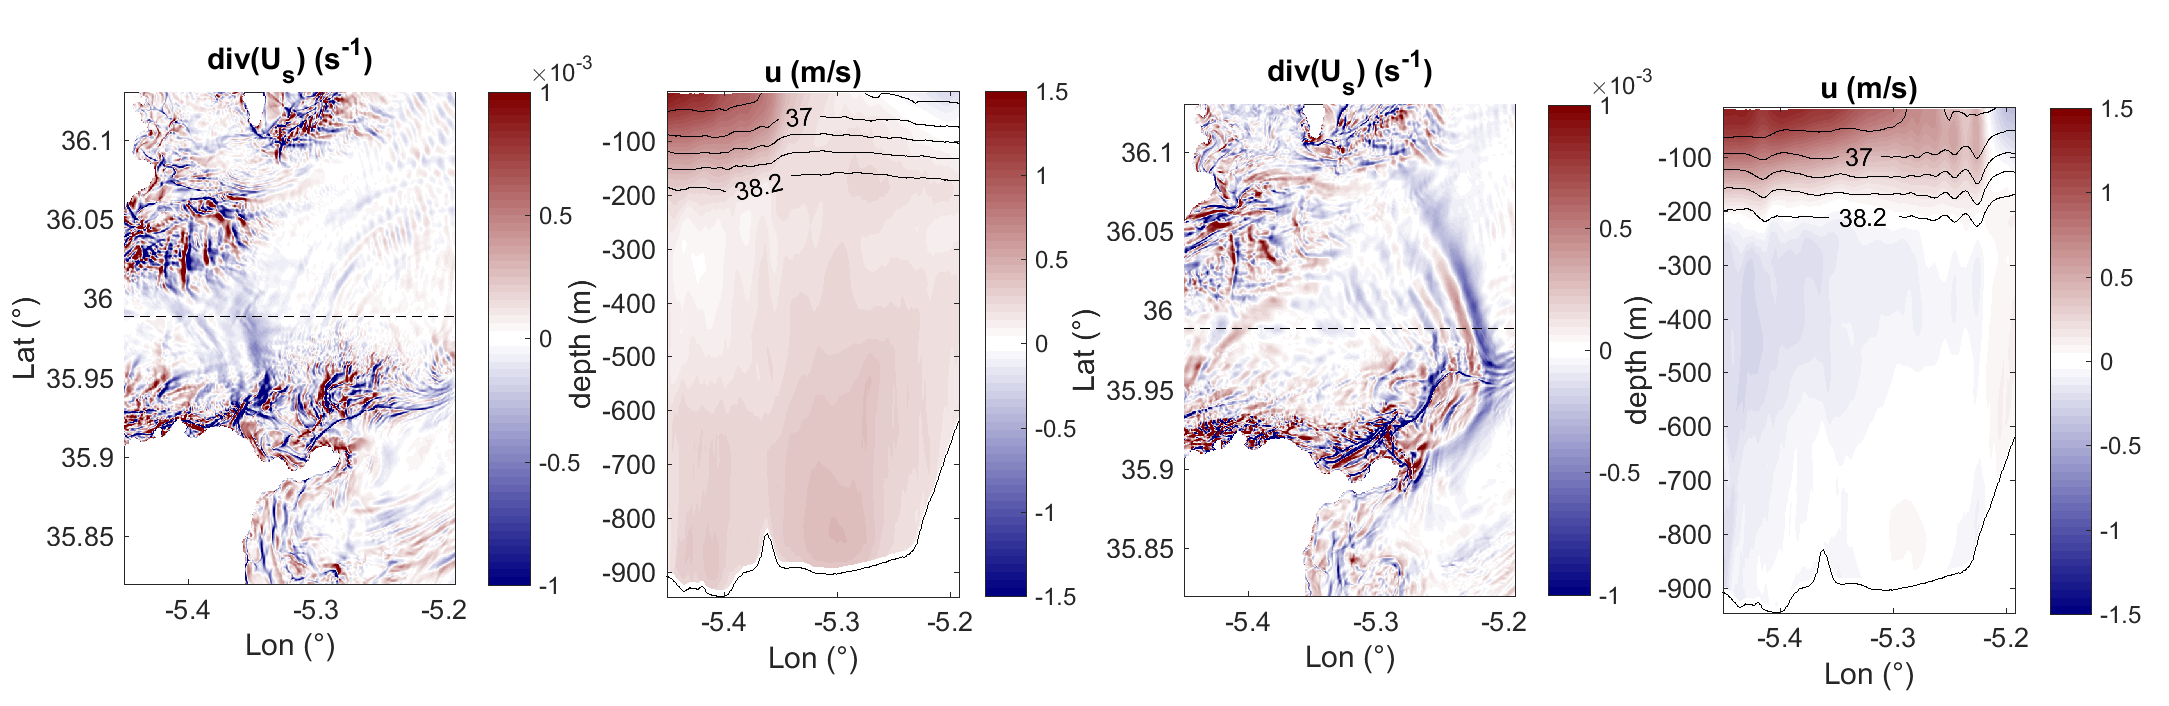
\includegraphics[width=1.\textwidth]{./GBR3D/coupesISW_ME2-2.png}
 \caption {Divergence of surface current (a,c) and vertical section (b,d) of salinity (black ishalines) and zonal velocity $u$ (color) in SimNT at 20h (a,b) and 22h (c,d) of simulation.}
  \label{FigISWNT}
\end{figure}



\begin{figure}[!h]
 \centering
%\begin{subfigure}{\linewidth}
%\centering
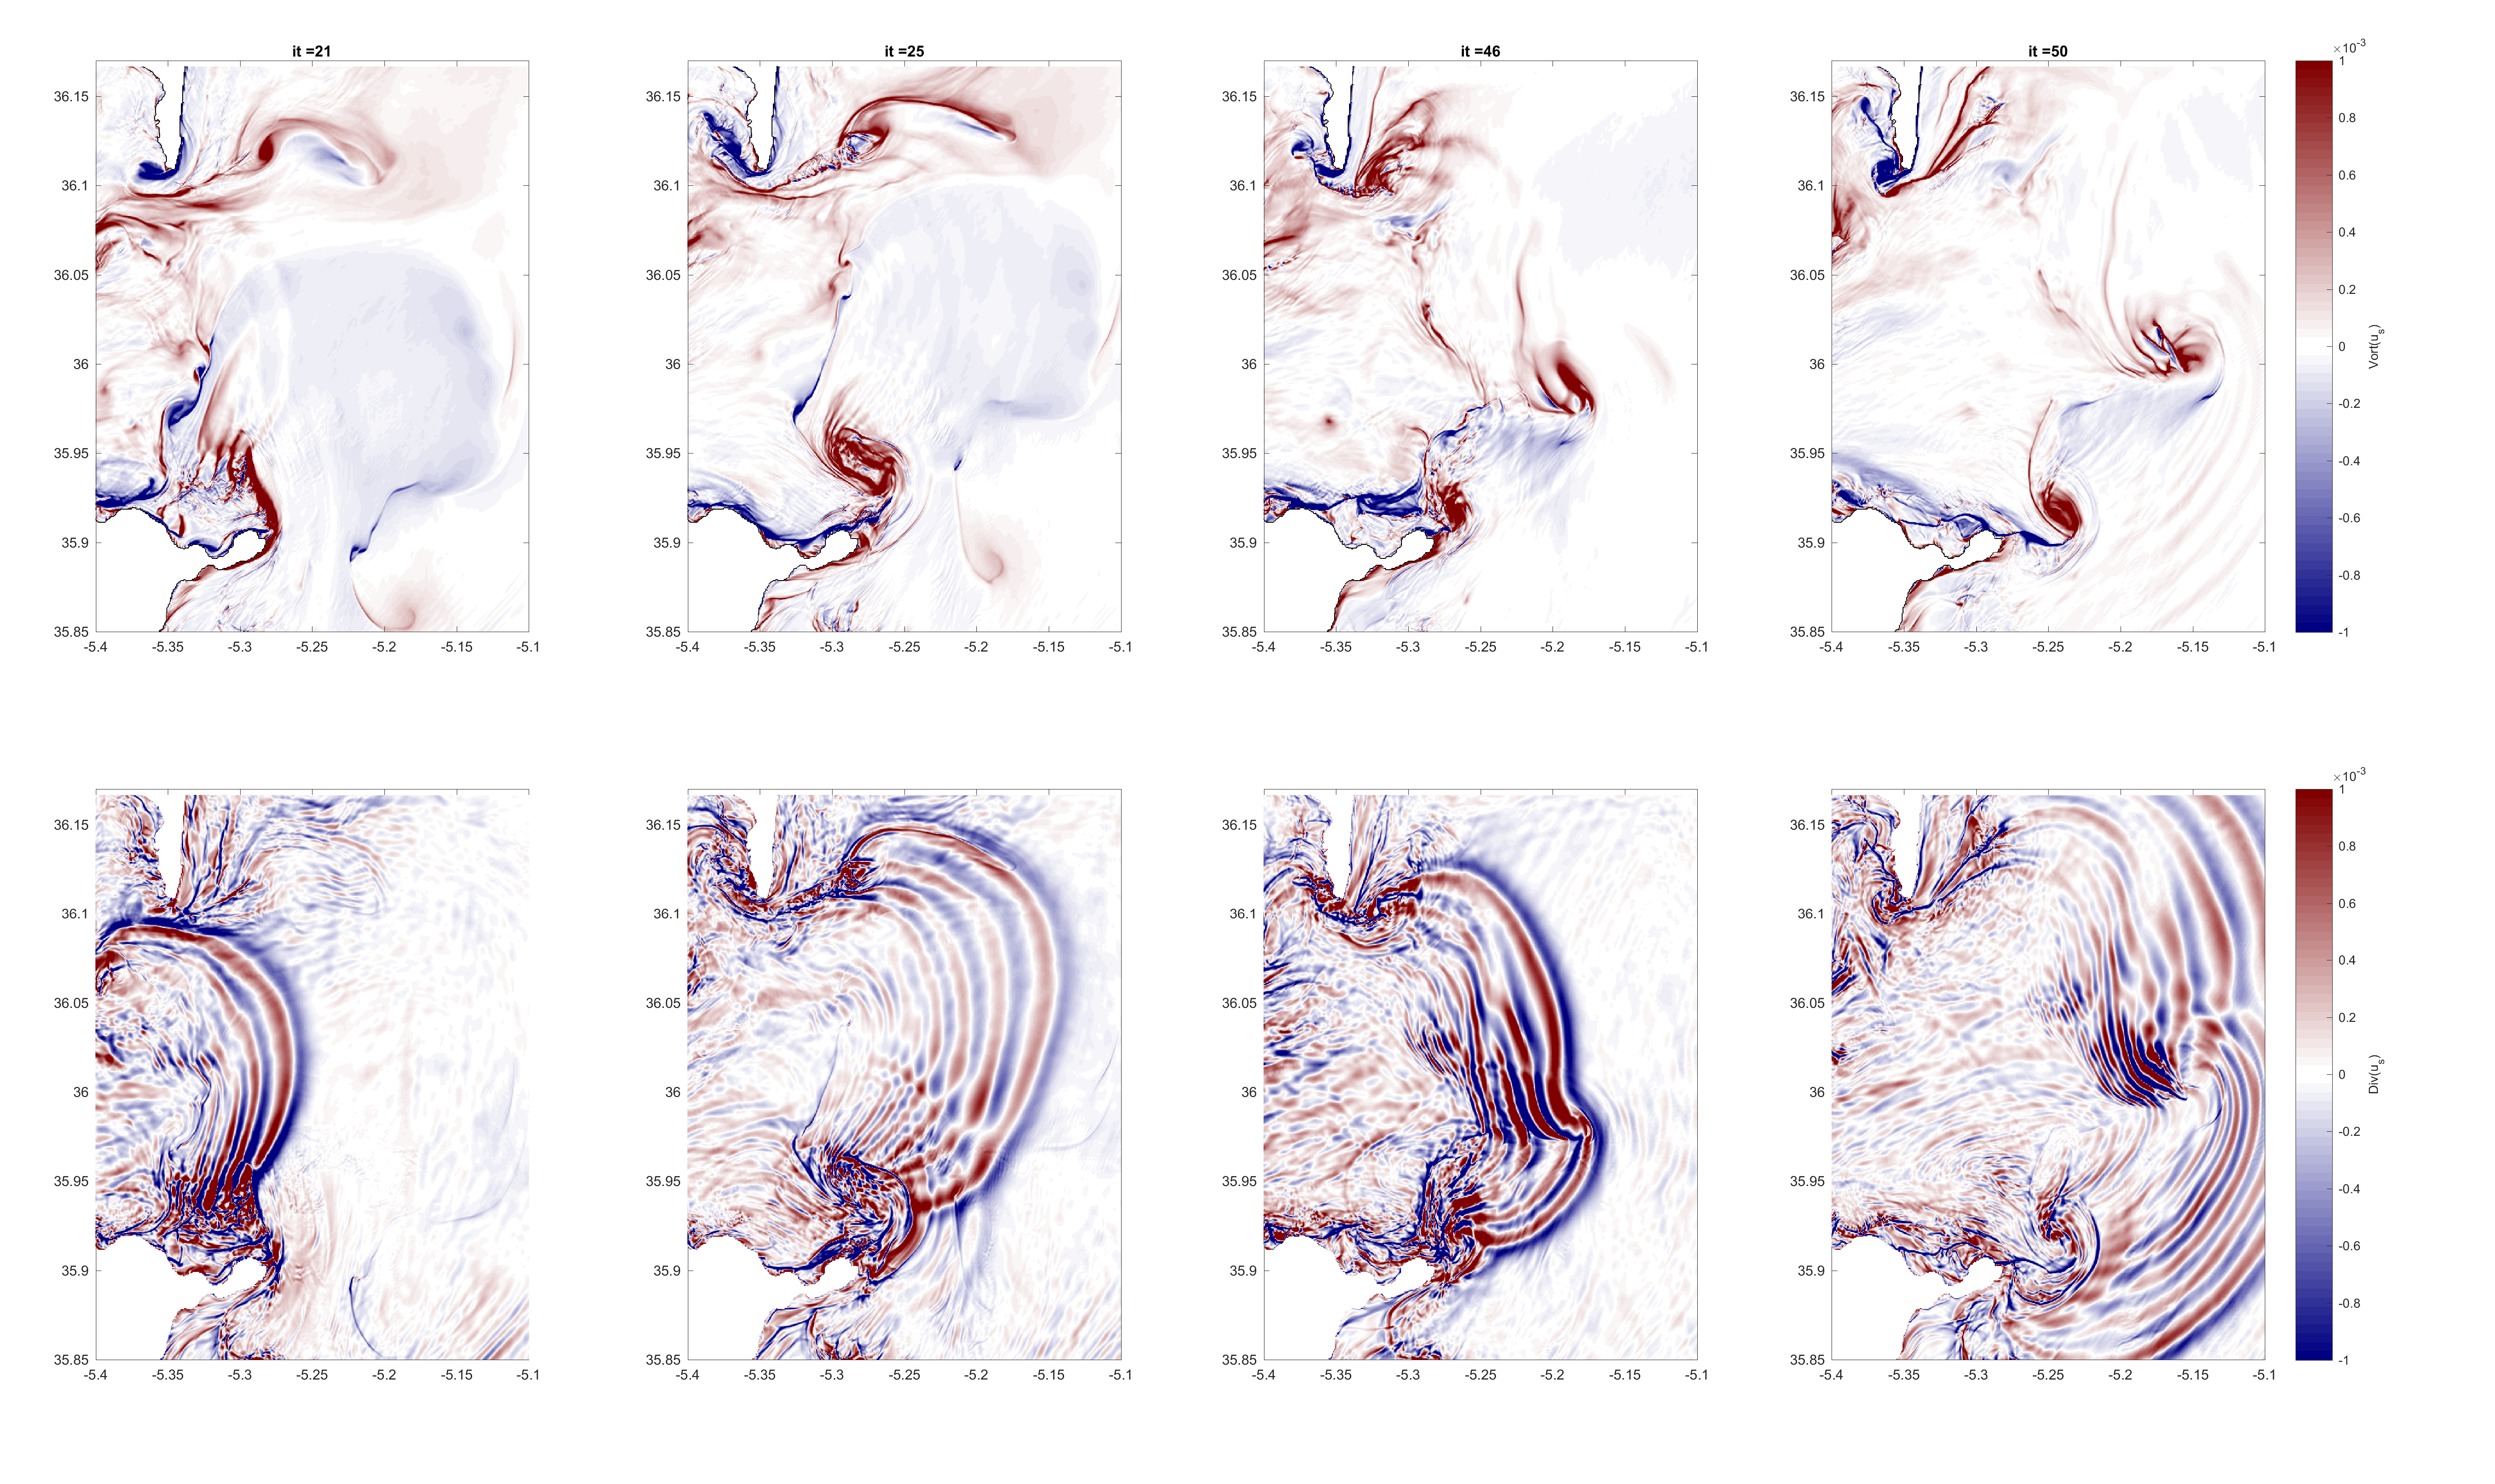
\includegraphics[width=\linewidth]{./GBR3D/FigTourbVE2.png}
%\end{subfigure}
 \caption {Divergence of surface current (upper row) at t=10.5H,12.5H, then 23H and 25H of simulation SimST,  and z-axis vorticity of surface current (lower row) for the same time.}
 \label{FigeddGBR3D}
\end{figure}

Solitary waves are observed as the relaxation of the hydraulic jump at CS as is the case in figure \ref{FigISWGBR3D}. Figure \ref{FigISWNT}.a and c also depicts the divergence of surface current but at the eastern exit of the Strait in inflow following a no-jump outflow. Figures \ref{FigISWNT}.b and d are vertical sections of zonal current and salinity at the same times. Can see that a train of solitary wave still ends up propagating in the alboran Sea, as the signal of the propagation of the baroclinic tide in figure \ref{FigISWNT}.b makes a more and more pronounced front with isohaline steepening due to non-linear effects. As is the case for the ISW generated at CS, non-hydrostatic dispersion balances this effect to create a train of solitary waves. In SimNT this process occurs following all \textit{no-jump} outflows.

However, compared to the upper row of figure \ref{FigeddGBR3D}, that also shows divergence of surface current but in tidal periods following hydraulic jump at CS, the train of solitary waves that are observed in Alboran Sea after a \textit{no-jump} outflow are less extended/have fewer waves. 

Figure \ref{FigeddGBR3D}.a,b then c,d show two inflows separated by one tidal cycle in simulation SimST. The lower row of figure shows the z-axis vorticity of surface currents at the same time. In the first two figures of each row, a train of solitary waves exits the Strait an enter Alboran Sea, the number of waves in the train increasing. A filament of positive vorticity is formed by interaction with the south coast in (e) and develops into a cyclonic eddy in (f). In \ref{FigeddGBR3D}.c one tidal cycle later the eddy is at 5.2$^\text{o}$W and 36$^\text{o}$N and the shape of the new train of solitary waves is refracted by this feature, south part accelerated and north part decelerated by the induced currents. At the same time can see once again vorticity patch off of Ceuta. In \ref{FigeddGBR3D}.d this patch too has developed in a cyclonic eddy that propagates in the Alboran Sea while the interaction between the solitary waves and the previous cyclonic eddy has resulted in an interference pattern in the wave packet. 


In the simulations, this process of generation of cyclonic eddy off of the coast of Ceuta occurs each time solitary waves exit the strait,  The wave of the next tidal cycle gets diffracted on this eddy, creating locally interference in the train of solitary waves.



\subsubsection{Dynamic at Camarinal Sill, primary instabilities}

\subparagraph{Neap-tide cycle}

Along with the features of the flow already discussed previously, figures \ref{FigHCN},\ref{FigHCS},and\ref{FigHCI} indicate patches of high standard deviation of parameter Q. They are the most extended for all outflow cases and for the spring tide inflow, although the values for this latter case are not as high and the patch is not as extended. High values of this parameter indicate oscillation of the value of parameter Q of greater amplitude, the highest are found for the two outflow case where hydraulic jump is detected (\textit{w-jump} and \textit{s-jump}), in the area west of CS at 5.79$^\text{o}$W and west of secondary bathymetric features in Tangier basin at 5.84$^\text{o}$W. There is also a lesser signal at Espartel Sill, of greater standard deviation for the spring tide outflow.

Figure \ref{FigTSCS}.a superposes to the standard deviation the singular vector of SVD performed on the 3D field of parameter Q computed during the outflow for the EOF that had the most high-frequency variability in its eigenvector, associated with propagation of vortices (the higher order EOFs (not shown) have low frequency variability and structure associated with the regional flow itself). As expected, the contour of parameter Q$=5e-5m^2s^{-2}$ in the EOF are located at same place as values of high standard deviation, on the west slope of Camainal Sill and the west slope of secondary sills in Tangier Bassin. 

Figures \ref{FigTSCS}.b to e show the partial view of $\theta$-S diagram of each gridpoint in the simulation at a given longitude, zoomed in on the part of the graph of med waters. See that in b that at 5.76$^text{o}$W, still over the crest of the sill, the repartition among mediterranean waters is still alike the one found in figure \ref{Fig_Ini_WM3D} at the east entry of the strait. Then from c to d, as look at more westward along the path of the mediterranean outflow, find the water parcels at close latitudes are homogenizing as three to four water masses.

These diagrams are plotted for longitudes close after the areas of high values of Q, where expected to have mixing processes, however not homogeneous water masses directly after CS. Look into it with 

\begin{figure}[!h]
% \centering
 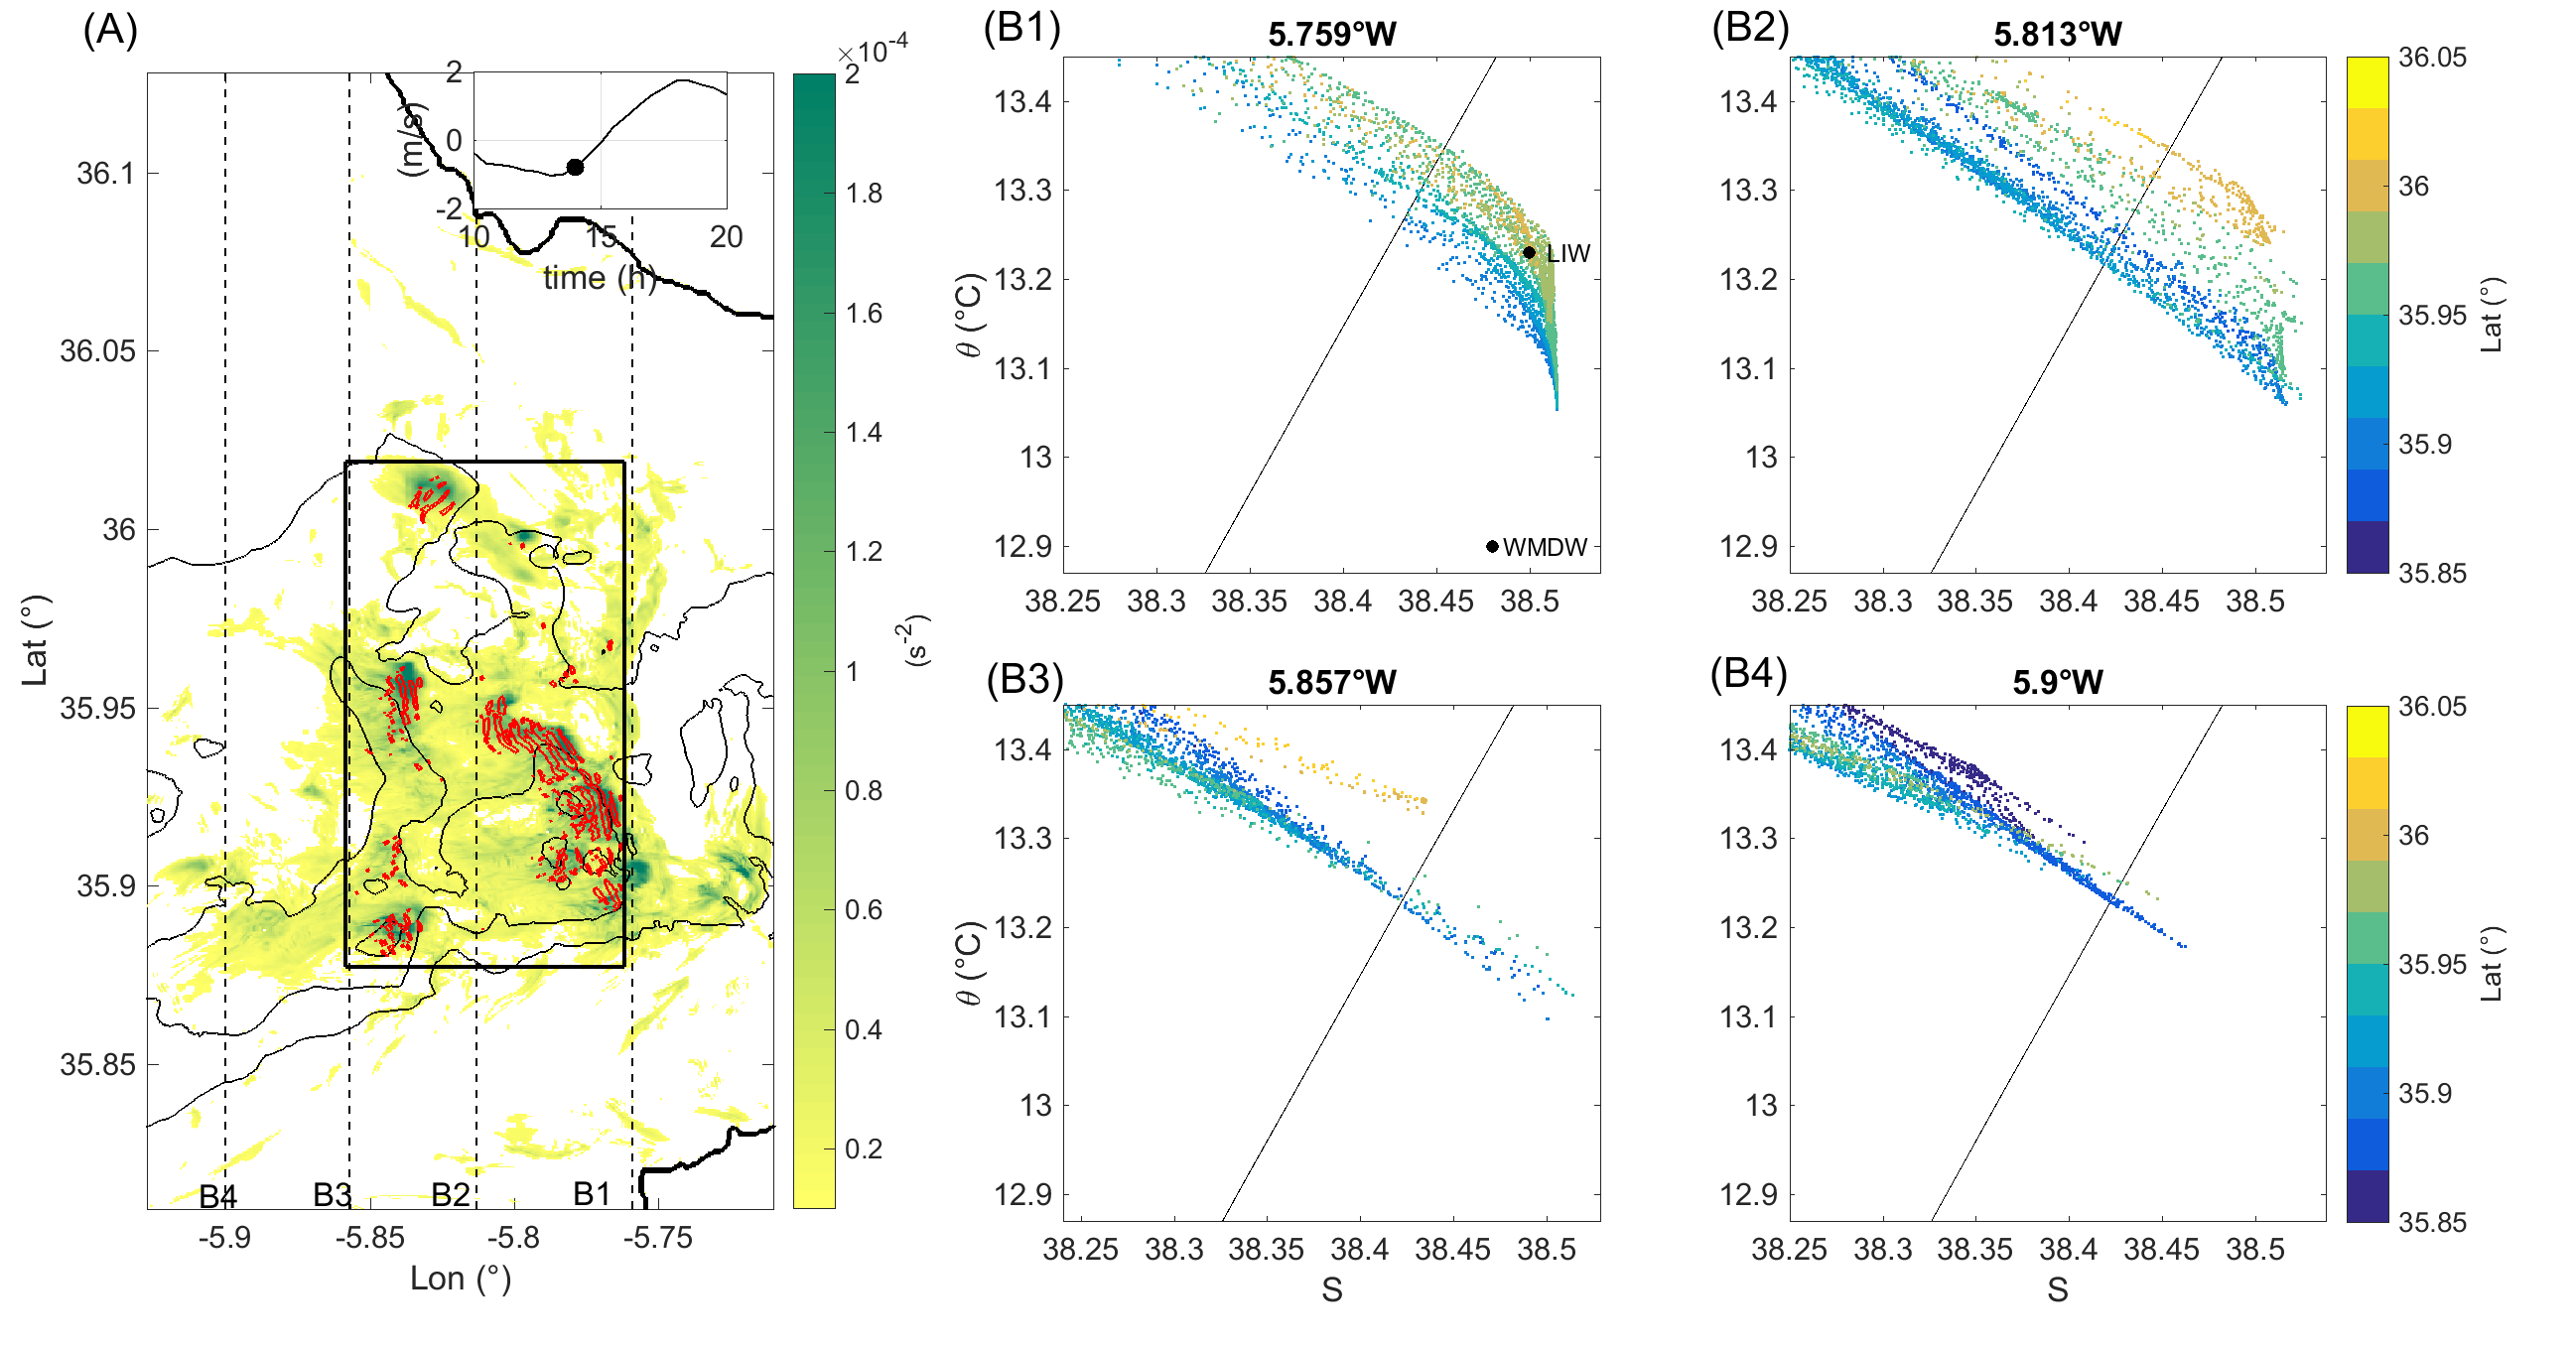
\includegraphics[width=\textwidth]{./GBR3D/TS_coupes_14H_VE2o.png}
 \caption {(a) Standard deviation of parameter Q over 30 mintues at t=14H in SimST (color) and trace of Q$=5$ from the high-frequency EOF of SVD performed in the rectangular black box during the outflow period. Black dashed lines indicate the longitude at which T,S diagrams are plotted. (b,c,d,e) T,S diagrams, zoomed in on area of Mediterranean watermasses. (Mettre LETTRES, rajouer section plus au sud?)}
 \label{FigTSCS}
\end{figure}


Now looking at the singular vectors of SVD for outflows of different strength of barotropic tidal currents . Figure \ref{FigEOFMIV}.a,b,c presents the EOF of parameter Q for the outflows of figures \ref{FigHCN},\ref{FigHCS},and\ref{FigHCI},along with vertical sections of salinity at the time of figure \ref{FigEOFMIV}d,e,f plotted along latitude 35.94$^\text{o}$N. Figure \ref{FigEOFMIV} g and h are histograms giving the height above seafloor and latitude of the grid points of the EOF for which Q$\geq 5e-5m^2/s^2$. On vertical sections, can see that the positive value of Q parameter are associated with billow structures of salinity that develop in the gravity current along the west slope of the Camarinal Sill. Those structures develop for each outflow case, but the wider distributions of height above sea floor and visualisation in the vertical section indicates the billows have greater radius in the hydraulic jumps cases, entraining more interfacial and atlantic waters into the mediterranean outflow. At this longitude where the instabilities are still developed, cores are not yet mixed in the simulation, can see as in the $\Theta$-S diagrams that the outflow is still heterogeneous.

The two hydraulic jump cases also differ, while instabilities develop along the same areas in no-jump and s-jump case, in the w-jump case the hydraulic jump and the start of the gravity current are co-localised at all latitude as seen in the vertical section, which adds a possible area of generation between 35.92$^\text{o}$N and 35.93$^\text{o}$N, down slope of the shallowest point of the sill where the flow of Mediterranean waters is not as strong for s-jump and no-jump cases.


\begin{figure}[!h]
% \centering
 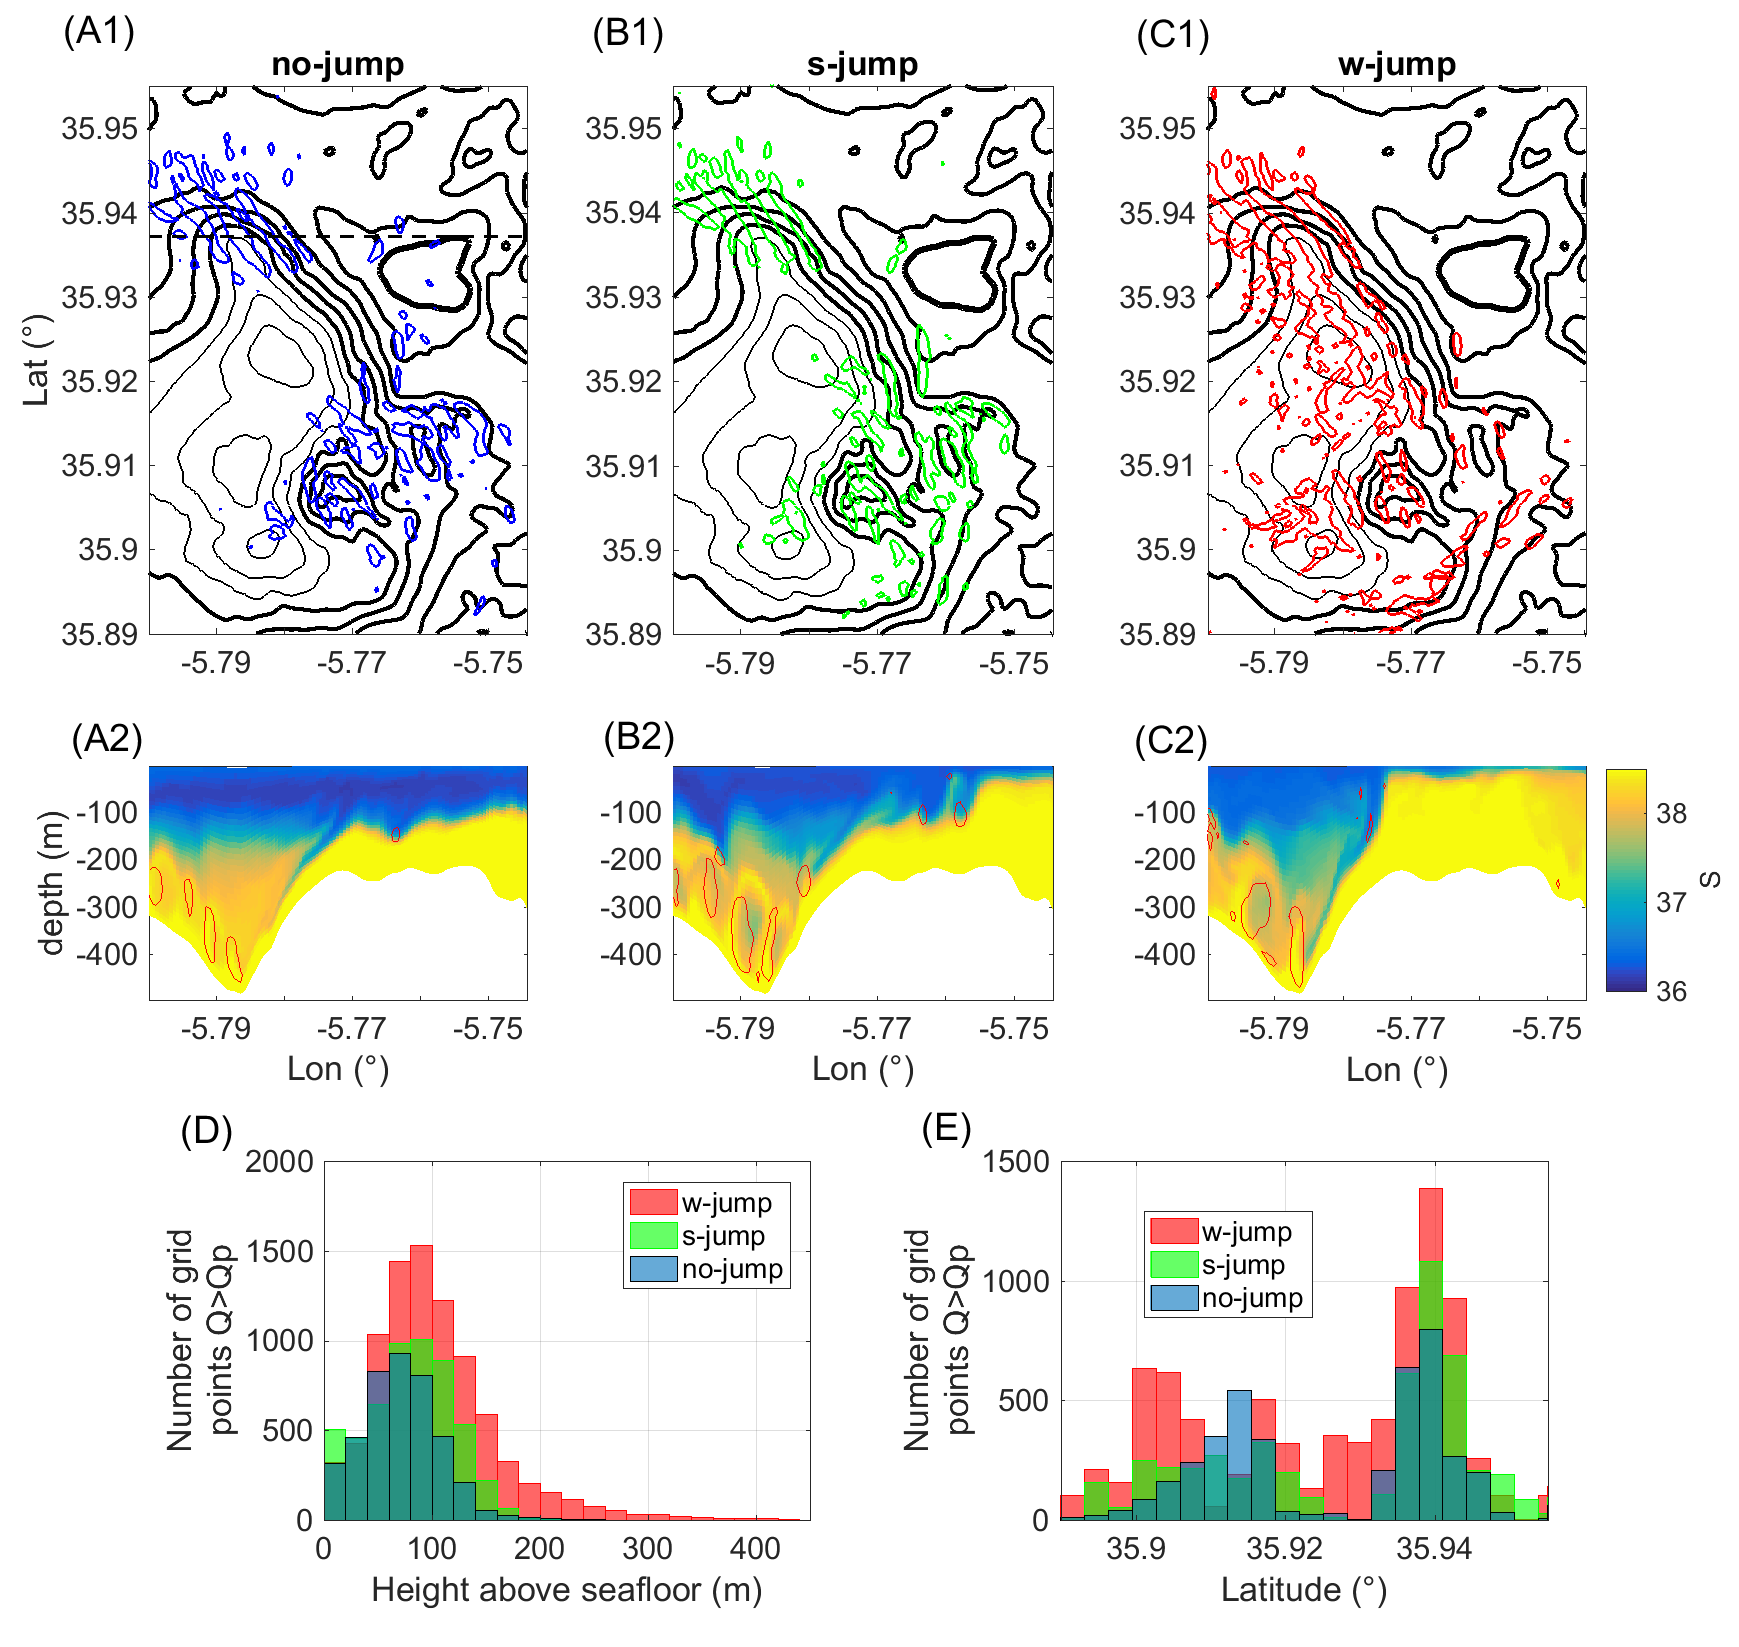
\includegraphics[width=\textwidth]{./GBR3D/EOF5_MIV_2D.png}
 \caption {(a,b,c) Contour of parameter Q$=5.10^{-5}$ in first high frequency EOF of SVD performed during outflow of figures \ref{FigHCN}.b,\ref{FigHCI} and \ref{FigHCS}.b respectively. and isobathes (black) (200m, thicker)  (250 to 450, thick) (500 to 600m, thin). (d,e,f) vertical section of salinity (color) and contour of Q-parameter $=5.10^{-5}$ at latitude $35.9372^\text{o}$ at the same time as figures \ref{FigHCN}.b,\ref{FigHCI} and \ref{FigHCS}.b respectively. (g) histogram of the height of the grid points of each EOF shown in a,b and c above the seafloor. (h) histogram of the latitude of the grid points of each EOF shown in a,b and c above the seafloar. }
 \label{FigEOFMIV}
\end{figure}


\subparagraph{Closure scheme}

Now look at four other simulations, three use Smagorinsky turbulent scheme with different coefficients. One is using GLS K-$\epsilon$. In figure \ref{Fig3Dsch}.a,c,e,g, vertical section of salinity during the first outflow at t$=$5h of simulation which is in a no-jump case, with Richardson gradient number $Ri$ and Q parameter indicated. $Ri$ is calculated from fields of density and velocity averaged over a half hour to filter out the propagating structures.

Figure \ref{Fig3Dsch}.b,d,f,h the averaged salinity in med (b,f) and atl layer(d,h),east (f,h) and west (b,d) of Camarinal Sill. Note that this is averaged value, as shown in figure \ref{FigTSCS} and can be seen in the vertical sections the outflow/med layer is not homogeneous at this longitude yet/those longitudes.


Looking at averaged layer salinities east of the Sill in figures \ref{Fig3Dsch} f,h, see that simulations SimIT-S001, SimIT-S01 and SimIT-Kep have same salinities for med layer, and can see some differences in atl layer punctually. , the simulations most different is SimIT-S1 that has a less salty med layer and a saltier atl layer. This is logical as with the enhanced mixing coefficient, more diffusion in the pycnocline between the two layers.

However, while the atl layer is again saltier west of the sill for SimIT-S1, so is the mediterranean layer, especially between 2 and 8 houyrs of simulation, which shouldn't be the case if only diffusion. Looking at the vertical section at 5 hours of simulation can see that instabilities develop for all of them. However, while can see that the area of $Ri=0.25$ starts at 5.77$^\text{o}$ for all four simulations, indicating shear instabilities could develop from this point in the gravity current, for simulation SimIT-S1 they start down slope of an intrusion of atlantic waters at 5.783$^\text{o}$W. While the other simulations, the salinity entrained by teh billows is from the altantic layer//contain less salty waters, ie the signal of atl surface water in the med outflow will be stronger in this simulation.

More atl waters incorporated for Kepsilon, for which the billows are not as developped, instabilitied less developed with smaller values of parameter Q (closer to a gravity current only?), and less salty outflow. This signal persists after $t=7h$ when the flow reverses and no more generation of instabilities, and in a lesser extent for SimIT-S1 for which the effect of more diffusion in the pycnocline may counteract with the injected med water.


While the width of the Med vein as it begins to go down slope of Camarinal as salty water is the same, in simulations 1 and 2 instabilities are earlier in the jump and bring more atl waters as the core or billows are advected down slope, resulting in more atl water being integrated to the med outflow at the passage of CS. 






\begin{figure}[!h]
% \centering
 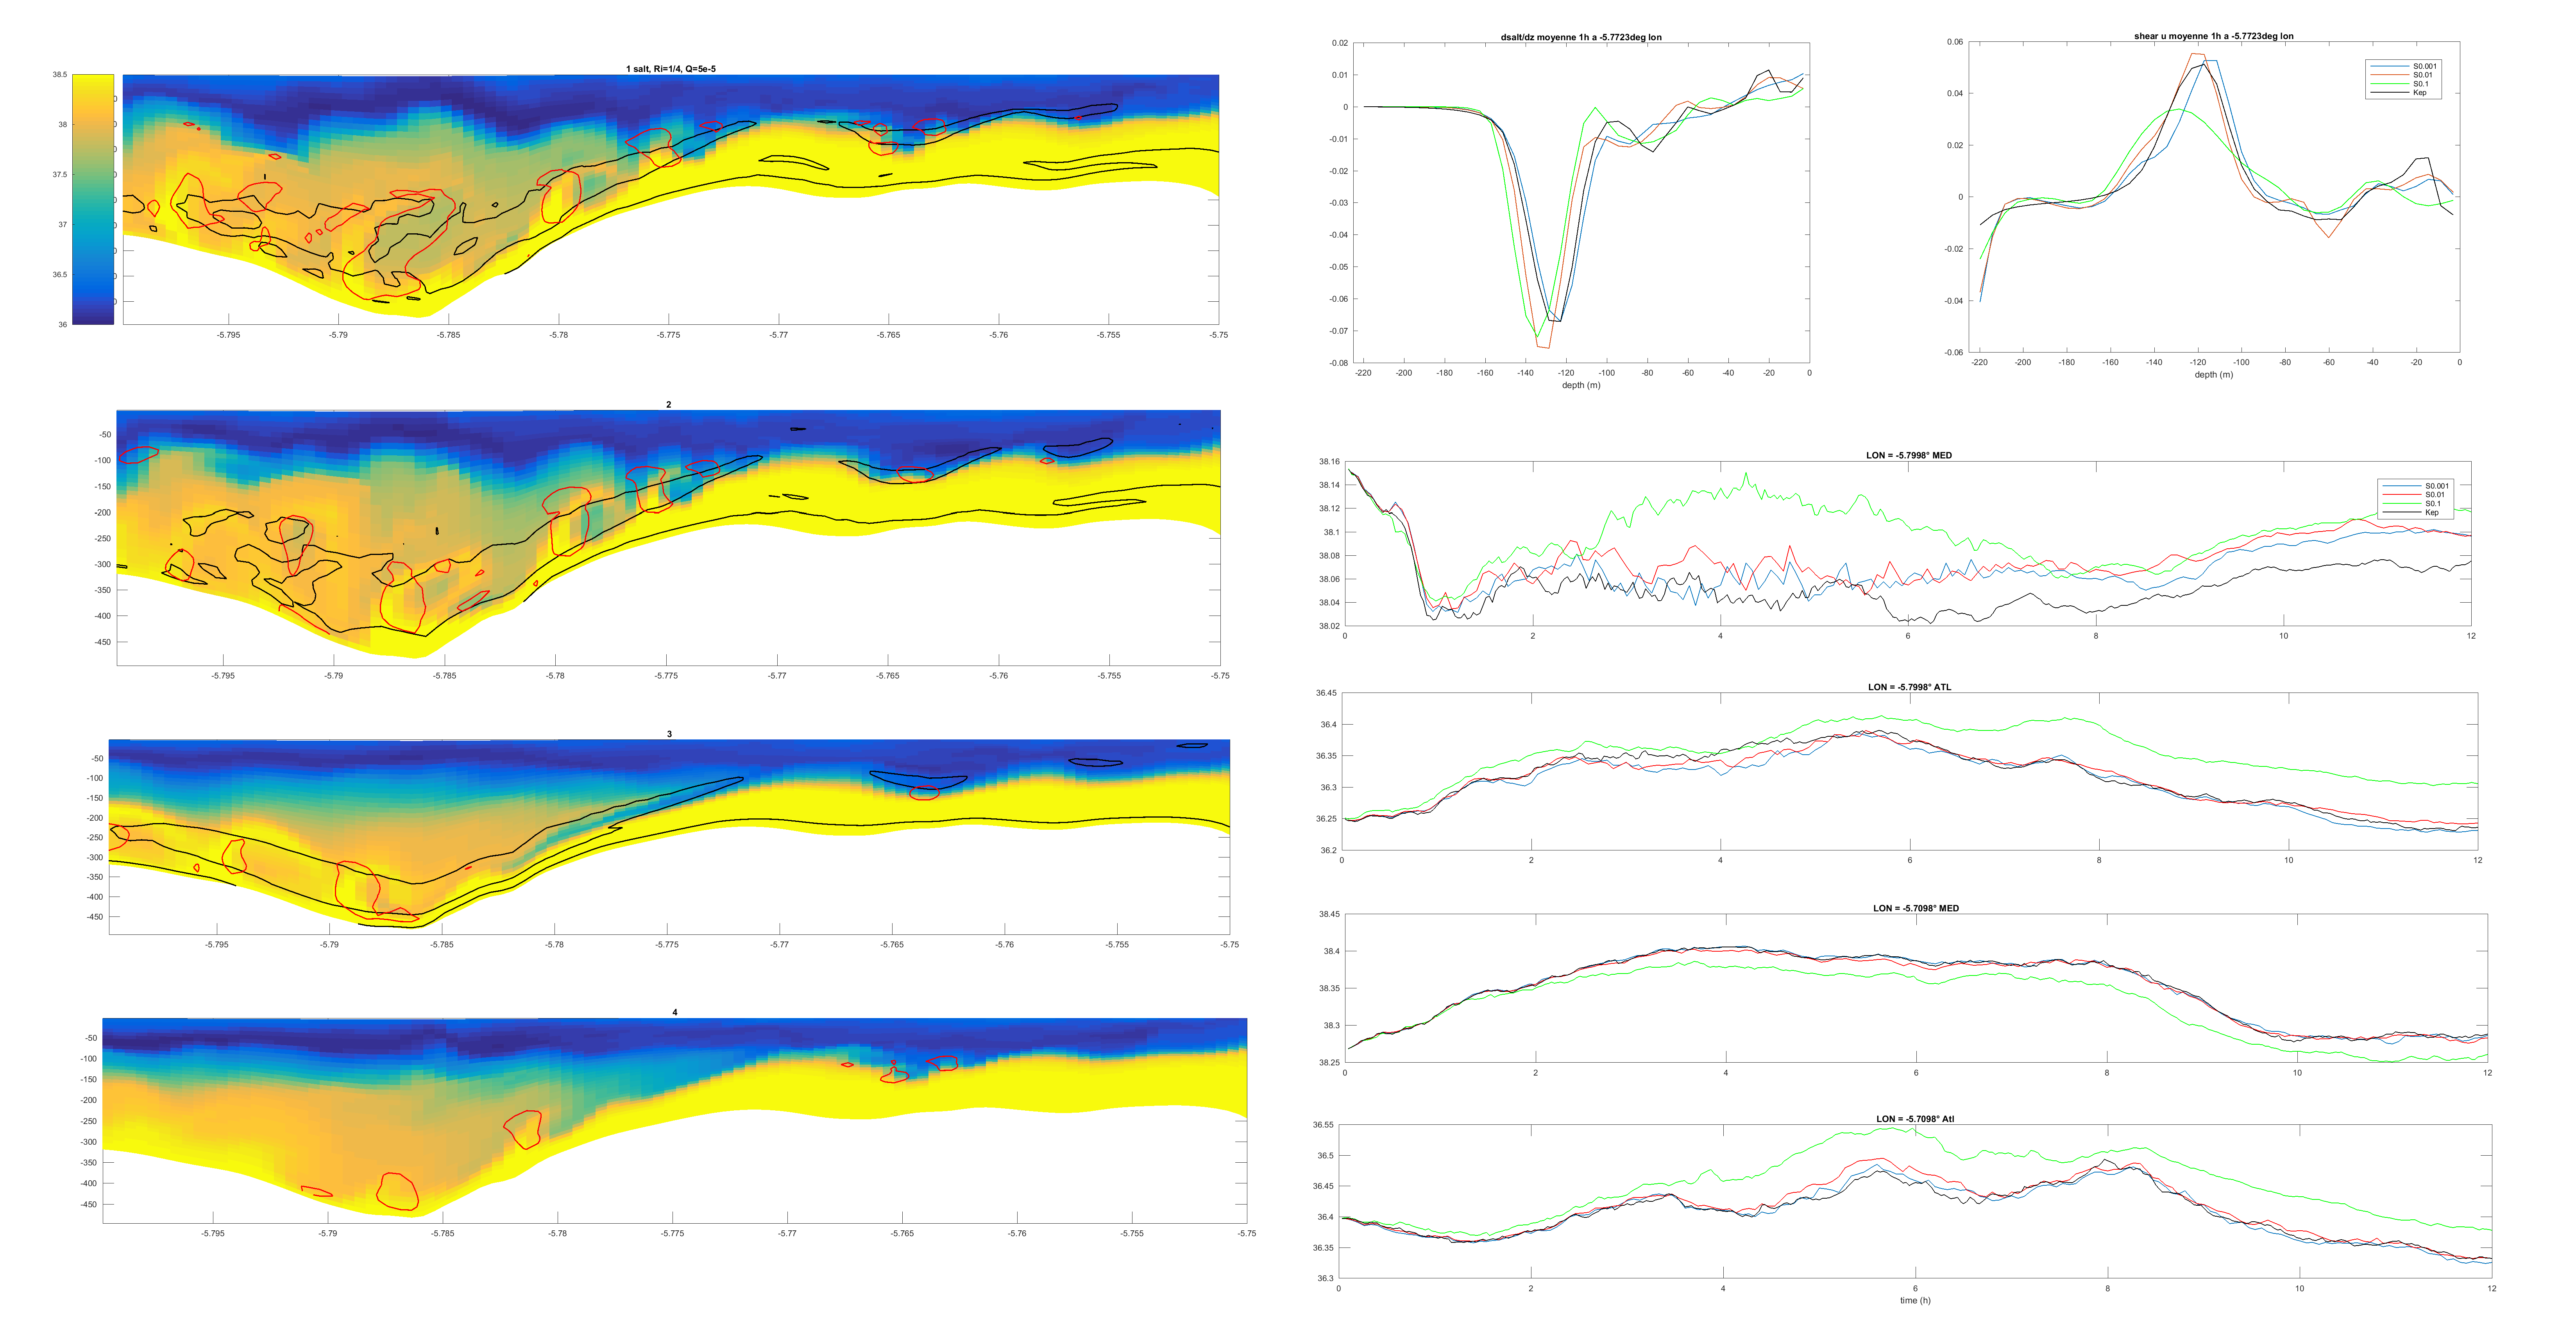
\includegraphics[width=\textwidth]{./GBR3D/Figsmago.png}
 \caption {Vertical section of salinity (color) and contour of $Q=5.10^{-5}$ (red) and Richardson gradient number $=025$ (black) at lat = $35.9372^o$ in simulations SimIT-S001,SimIT-S01,SimIT-S1 and SimIT-Kep IES at t=4h of simulation. time  (1:S0.001  2:S0.01  3:S0.1 4:Kep)(Rajouter une évolution de ubar!!! sur s0.001)}
 \label{Fig3Dsch}
\end{figure}

%-------------------------------------------------------------------------------------
\subsection{Conclusion}

Have looked into the variability in neap-spring tidal cycle of hydraulic control and other features in high resolution non hydrostatic simulation of the strait of Gibraltar.See no permanent supercritical flow across the simulations, only intermittent with the tidal cycle, with location and extension of the area of supercritical flow depending on the strength of the barotropic currents.

In outflow when both atl and med layers are critical, hydraulic jump, which position is either over the shallowest part of the sill, or over its western slope. This hydraulic jump evolves into train of solitary waves, as expected once hydraulic control is lost near high tide, that exits the strait into the Alboran Sea. Even for tidal cycle for which the flow over the sill is not critical and there is no formation of hydraulic jump, the non-linearity of the propagation of the barotropic tidal signal in the eastern part of the strait devolves into a less extended train of solitary waves propagating into the Alboran Sea.At each simulated tidal cycle, a cyclonic eddy is formed of the coast of Ceuta in the southern part of the eastern exit of the Strait. This eddy is advected by the flow in th Alboran Sea and interacts with the train of solitary waves, locally diffracting the waves.


Other feature present in simulations are the billows/shear instabilities developing in the lee of CS. In simulations, these billows are associated with high positive values of parameter Q that is used as proxy for their detection and analysis. The billows are generated at interface of med and atl waters and advected by the med outflow.   they are also present at secondary relief in tangier basin and at espartel sill. They are present during outflows of all intensity, but their repartition will change with intensity of tidal currents. They have a role in the way the med water is mixed, with changes of hydrological features of the med vein, and in simulation the way this mixing occurs is sensible to the dynamic of the instabilities that is piloted by the turbulent dissipation scheme.


 Can see that the configuration of the flow at CS, by being the first passage of the Med waters, will affect the hydrological properties of the Mediterranean outflow, first by the volume of med waters that can flow west of the sill at each outflow, second by how much Atlantic waters are being mixed into it.

However, it is important to note that simulation only represents the beginning of the mixing by turbulent processes, in particular, no secondary evolution of KH instabilities.


Moreover, The lack of atmospheric forcing probably means inaccuracies of features of the upper layer, especially circulation of the Atlantic layer in Tarifa Narrows where wind stress affects the upper layer. This could explain why have the baroclinic tide degenerate into an internal bore then a train of solitary waves for all inflows following a \textit{no-jump} outflow at CS, whereas observations indicate that in neap tide do not have solitary waves at each tidal cycle. Other processes could be affected like the formation of eddy at the exit of the Strait that occurs at the coast and its advection into Alboran that is probably influenced by the WAG.

%%\selectlanguage{french}

\hypersetup{pdfborder=0 0 0}


%-------------------------------------------------------------------------------------
%\section{Comparison of solitary waves and associated signal from in situ data}
\section[A first evaluation of LES with in-situ \& remote observations]{A first evaluation of LES with in-situ \& remote observations}
\label{sectionCampagne}

The pertinence and the accuracy of the high-resolution Large Eddy Simulations performed so far crucially need to be evaluated based on in-situ or remote observations of both the regional and fine scales of the real ocean. The observation of the latter is somehow difficult at least when these fine scales are localized in small, transient spots. In turn, LES can then appear as a well-adapted tool to help designing the campaign.

In the present section, only a selection of in-situ and remote observations of Gibraltar 2020 campaign is studied. While the exploitation of campaign data is incomplete, some observations are still presented to represent the complete work that was carried out during my Ph-D to provide an as-rigorous-as-possible work including both development of LES, investigation of LES dynamics and evaluation with dedicated observations. Further treatment of in-situ observations and the preparation of the Gibraltar 2022campaign are still being carried out.

\subsection{Field campaign Gibraltar 2020 (an overview)}
The field campaign of in situ measurements Gibraltar 2020 has been carried out by SHOM during the fall of 2020 in the Strait of Gibraltar and inthe western part of the Alboran sea aboard the research and survey ship \textit{L'Atalante}. This campaign and the following Gibraltar 2022 campaign are part of the PrometeVs program and LEFE-GEPETO project. On-site measures were taken by ship-based instruments from 8/10/2020 to 20/10/2020. Among those, sampling of the water column at both end of the strait were realized; at the eastern end of the strait on the 14th and 15th October, and at its western end on the 16th of October.

Additionally, five moorings were deployed as presented in table \ref{tab_moor}, locations are also indicated in figure (\noparref{fig_moor}.A2). Mooring M1 is positioned west of the slope of Camarinal Sill. Mooring M3 is placed in the southern deep half of CS whereas M2 is positioned in a shallow area at the center. M4 and M5 are positioned near each other at some distance east of CS. Three of the moorings (M1, M3 and M5) are equipped with CTD sensors to provide hydraulogical characteristics of the water masses, and the other two (M2 and M4) with ADCP sensors to sample the currents in the water column. Sampling frequencies range from a few tens of seconds to one minute.

\begin{table}[!h]
        \centering
        \begin{tabular}{|c|c|c|c|}
                \hline
                Mooring & type & position & date (UTC)\\ 
                 \hline
                M1 & CTD & 35° 55.264'N ; 5° 46.739'W & 8/10/2020 15h - 9/11/2020 12h\\
                M2 & ADCP & 35° 55.761'N ; 5° 45.288'W & 8/10/2020 5h - 17/10/2020 15h\\
                M3 & CTD & 35° 54.719'N ; 5° 44.459'W & 8/10/2020 13h - 22/10/2020 21h\\
                M4 & ADCP & 35° 55.870'N ; 5° 41.020'W & 8/10/2020 7h - 17/10/2020 14h\\
                M5 & CTP & 35° 56.229'N ; 5° 41.026'W & 8/10/2020 9h - 1/11/2020 14h\\
                \hline
        \end{tabular}
        \captionof{table}{Name, type of sensors, coordinates and date of deployment for moorings during Gibraltar 2020 field campaign.}
        \label{tab_moor}
        %\end{minipage}
\end{table}
In section \ref{section_obs_moor}, mooring data from M2, M4 and M5 are analyzed for a first observation period covering the ten-day period 8/10 to 18/10 during which, as indicated in table \ref{tab_moor}, both types of moorings data are available.


\subsection{Insights from LES simulations in preparation of Gibraltar 2020}

The numerical simulations presented in section \ref{sectionSim3D} are based on a high-resolution, non-hydrostatic model. Atmospheric fluxes are neglected as a first step toward realistic, high-resolution Large Eddy Simulation of the region of Gibraltar strait. This simulations provide information on the flow and processes occuring in the strait that were used to eâre the Gibraltar 2020 campaign.

 
\begin{figure}[!h]
% \centering
 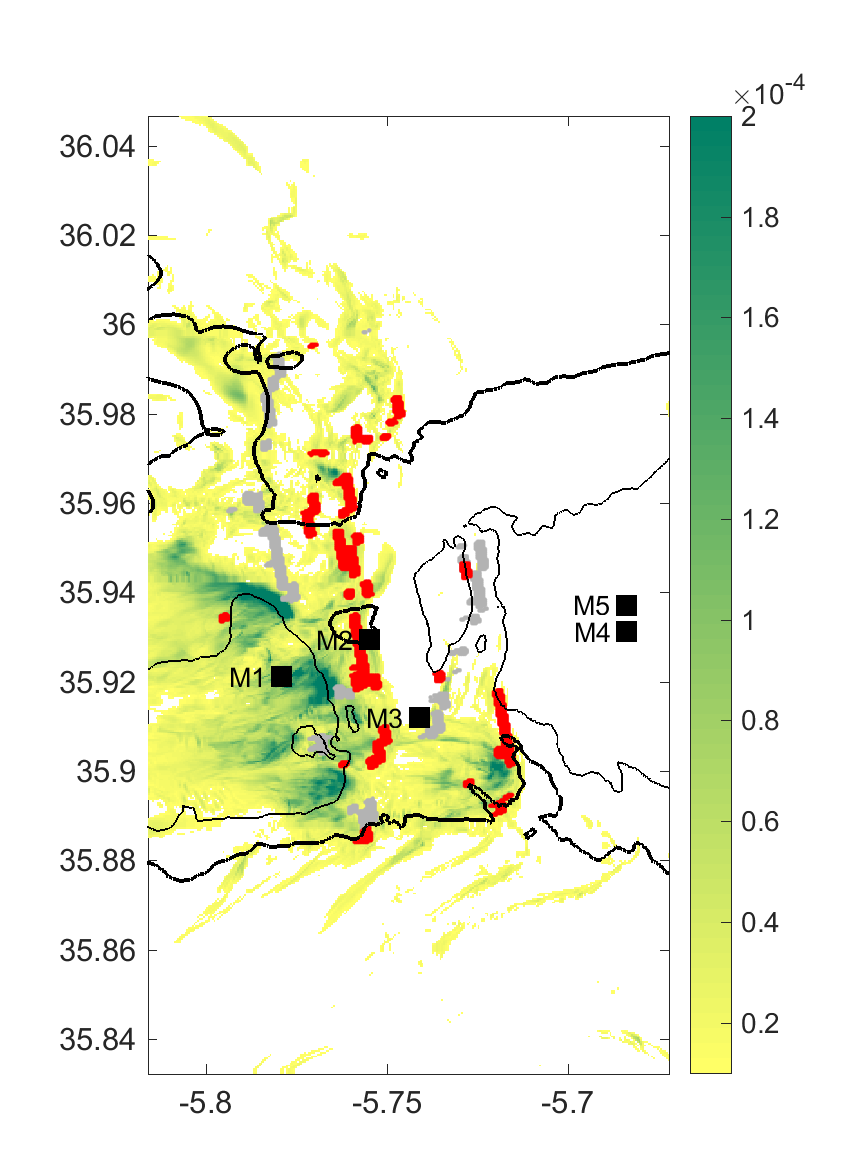
\includegraphics[width=\textwidth]{./GBR3D/Fig_Moor.png}
 \caption {(A1) Water column sampling sites fot (B1) and (B2). (A2) locations of moorings deployed during Gibraltar 2020 (black squares), over the map of standard deviations of parameter Q (colorbar) and the location of the hydraulic jumps of w-type and s-type from high-resolution numerical modelling of the strait of Gubraltar, as presented in section \ref{sectionSim3D}. (B1 and B2) $\Theta$-S diagrams for the series of water column sampling carried ou respectively at the western and eastern exit of the Strait, water mass definitions according to \color{red}\citet{najanro_2014}\color{black}.}
 \label{fig_moor}
\end{figure}

The field of standard deviation of parameter Q and the localization of the hydraulic jumps in figure (\noparref{fig_moor}.b) are for instance issued from those simulations. In combination with external restrictions such as the dense maritime traffic, strong currents and steep slopes of the area, such diagnosis and others were studied to chose the mooring deployment as well as the transect plans for the campaign (not shown). As an example, M1 was positioned down the western slope of the sill, i.e. downflow of a potential primary instability generation area (see section \ref{PartDiag3D} and \ref{section3DResFlow} for a discussion of this diagnosis in high-resolution numerical simulation).

Figure (\noparref{fig_SARIES}) features a comparison between a SAR image (figure (A)) of the strait of Gibraltar with the surface signature of a propagating ISW just east of CS, and the corresponding field of norm of the gradient of surface currents in SimIT at the same date (figure (B)), showing a traveling wave in the same vicinity. Whereas the shape of the train itself differs in the model and observed fields, the simulation gives an accurate idea of the propagation speed of ISWs in the strait of Gibraltar. This was used to predict the position of ISW in relation to the tidal cycle as predicted by the spanish institute Puertos del Estado\footnote{http://www.puertos.es/}. The anticipation of position of ISWs train was accurate at least in the strait of Gibraltar itself. In the Alboran Sea, where the influence of the gyre on the form of the wave packet is important, prediction was not as accurate, with time of arrival being greatly delayed compared to our predictions. 

Beyond the propagation speed, the high resolution of the model means that the shape of individual solitary waves is accurate as it propagates. This is used in the following section \ref{section_obs_moor} to help in the interpretation of mooring data from M4 and M5.


\begin{figure}[!h]
% \centering
 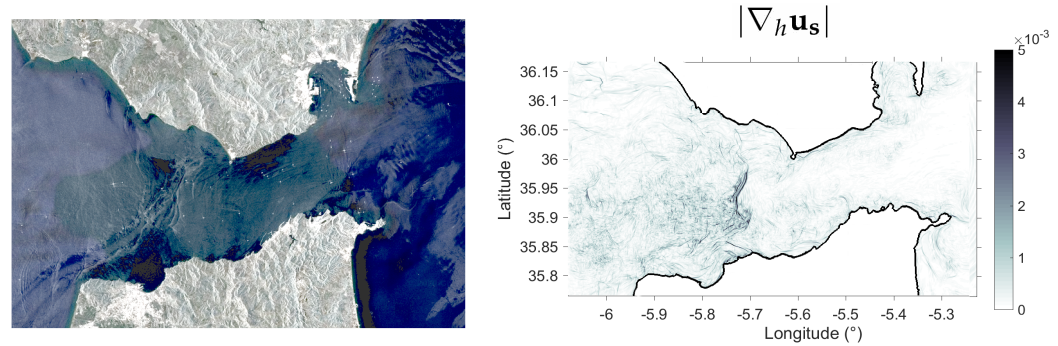
\includegraphics[width=\textwidth]{./GBR3D/Comp_SAR_IES.png}
 \caption {(a) Sentinel-1 Synthetic Aperture Radar (SAR) image (12/09/2017 - 6h18pm UTC). (b) Norm of the gradient of surface horizontal velocity (s-1) in the simulation SimIT (12/09/2017 - 6h30pm or t = 35h30 in simulation time) presented in section \ref{sectionSim3D}.}
 \label{fig_SARIES}
\end{figure}


\subsection{Overview of the mesoscale circulation during the observation period}

The in-situ time period covers one (for ship-based instruments and ADCP moorings) or two (for CTD moorings) neap-spring tide cycles. Figure (\noparref{fig_moor_US3}.B) shows the depth-averaged zonal component of the current measured at CS (data from M2 mooring). The measures begin during the neap-tide part of the fortnightly cycle. The west Alboran Gyre was also present in the West Alboran Sea during the field campaign (not shown). 

Figure (\noparref{fig_moor}.B1 and B2) present the $\theta-S$ diagram from ship-based water column sampling. For both figures, each color refers to a different sampling station indicated in figure (\noparref{fig_moor}.A1).

On the west end of the strait (figure (B1)), no Mediterranean water was sampled at the southernmost station and a well-mixed signal could be identified at the northernmost station, delimiting the path of the Mediterranean outflow between 35.7$^{\text{o}}$ and 36$^{\text{o}}$ N. Among the signals of Mediterranean outflow waters, the two northernmost stations that reach depths shallower than 400 m (orange and yellow) show an enhanced mixing with NACW.

On the east end of the Strait (figure (B2)), WMDW can be found at depth for all stations except the northernmost (yellow). For the next two stations south of the latter, as well as the two southernmost stations, WMDW is mixed with intermediate waters. 

The five northernmost stations' surface waters are fresher waters than the SAW signal at the rest of the stations. This could be due to the northern stations being affected by the upwelling from the Iberian coast. The intermediate Mediterranean waters sampled at these stations are also warmer and saltier compared to the signal of the remaining four, which is interpreted as LIW.


\subsection{Solitary waves at M4 and M5 mooring and currents over CS at M2 mooring}
\label{section_obs_moor}

\begin{figure}[!h]
% \centering
 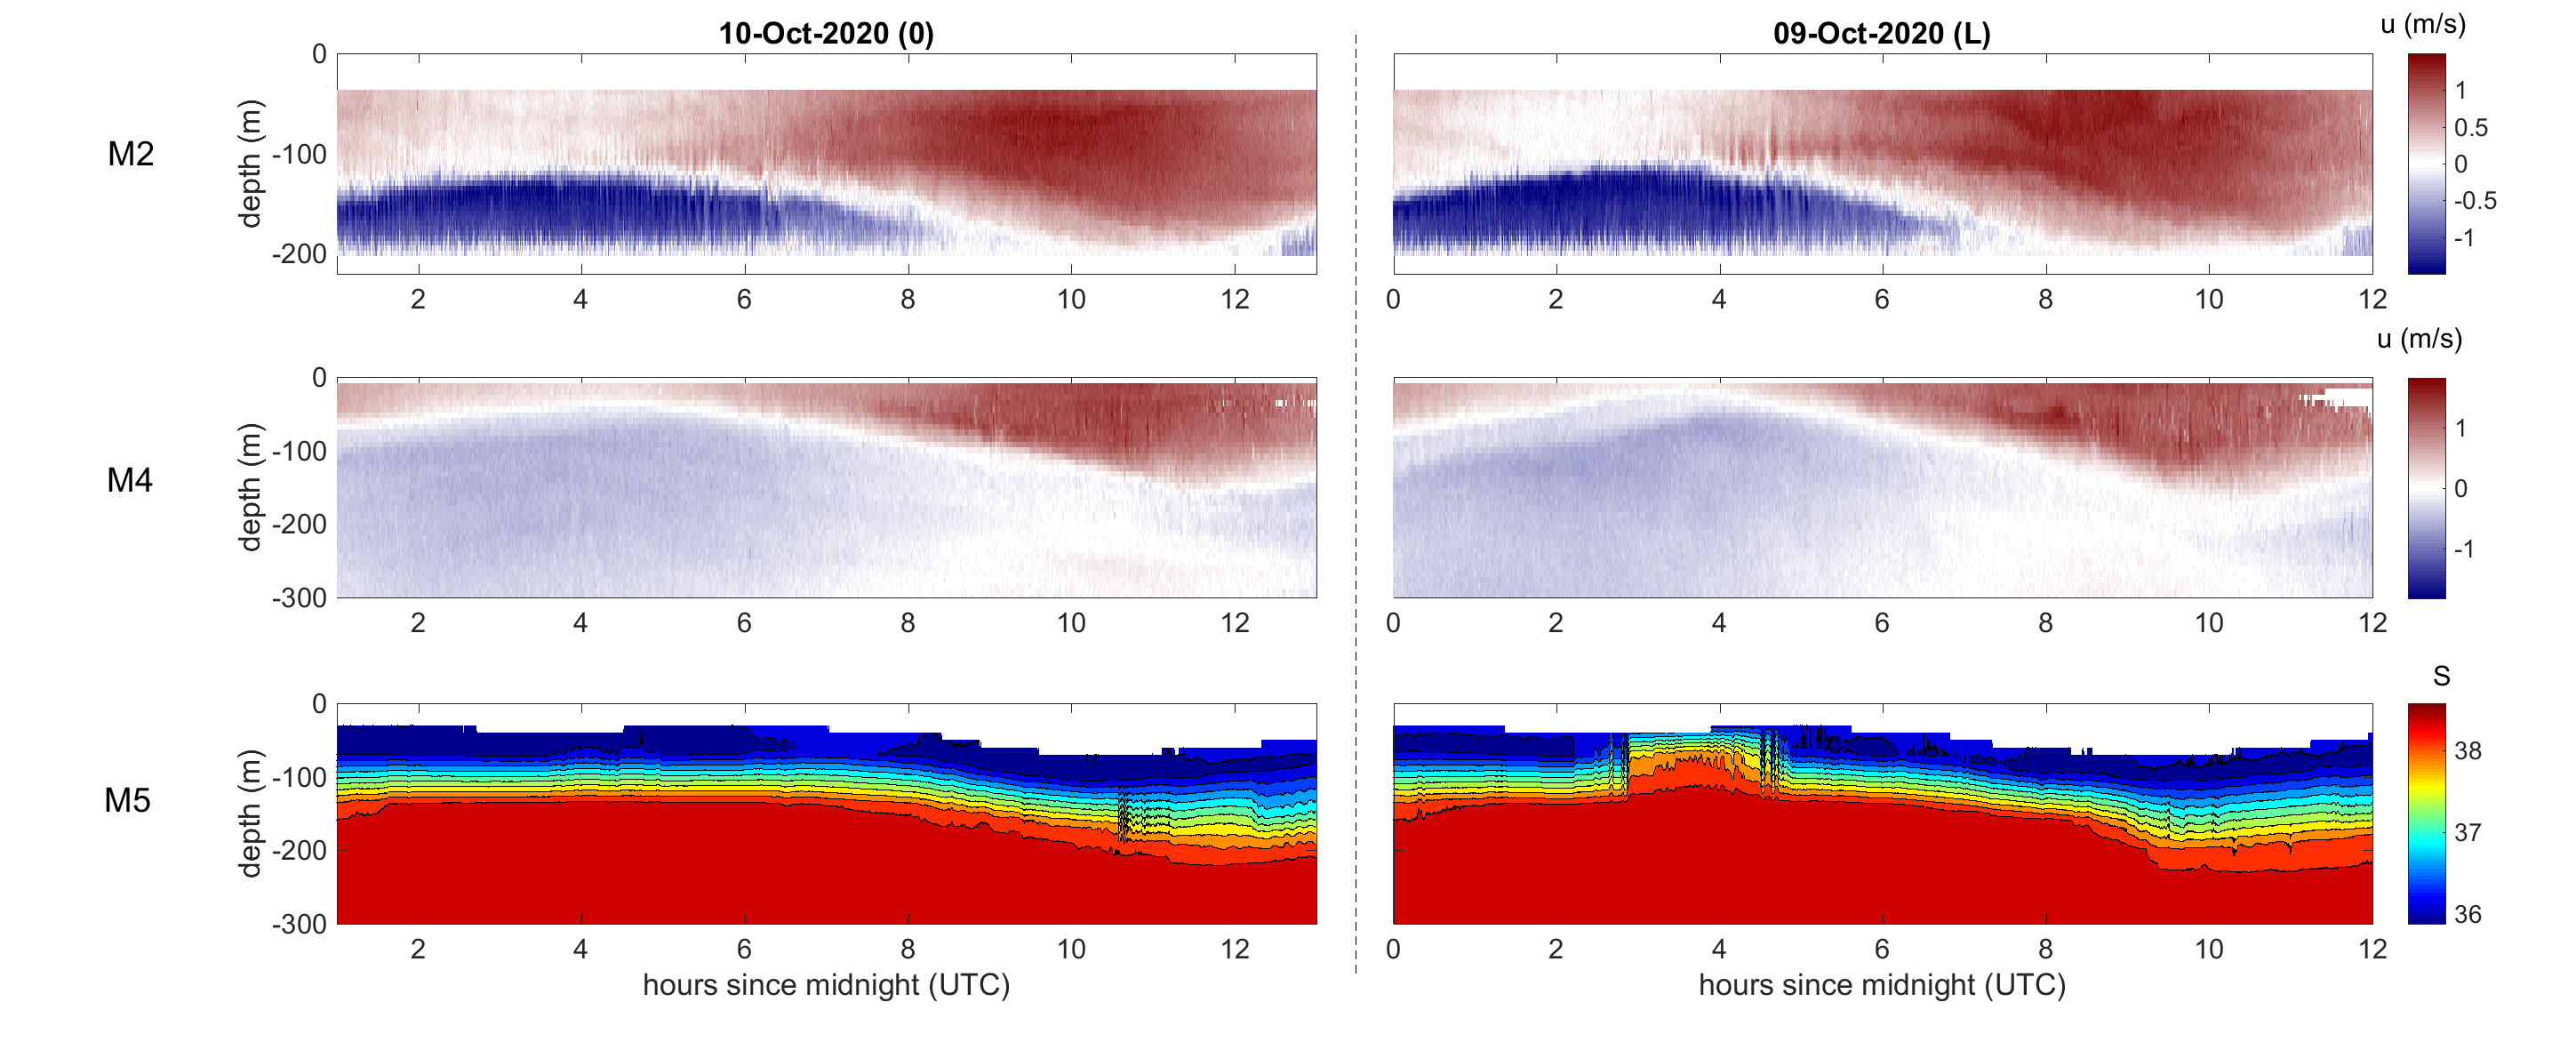
\includegraphics[width=\textwidth]{./GBR3D/US_moorings1.png}
 \caption {timeseries of mooring data over the water column from M2 (upper row), M4 (center row) and M5 (lower row) mooring. The zonal component of currents is represented for M2 and M4 mooring, and the measured salinity at M5 mooring.}
 \label{fig_moor_US1}
\end{figure}

\begin{figure}[!h]
% \centering
 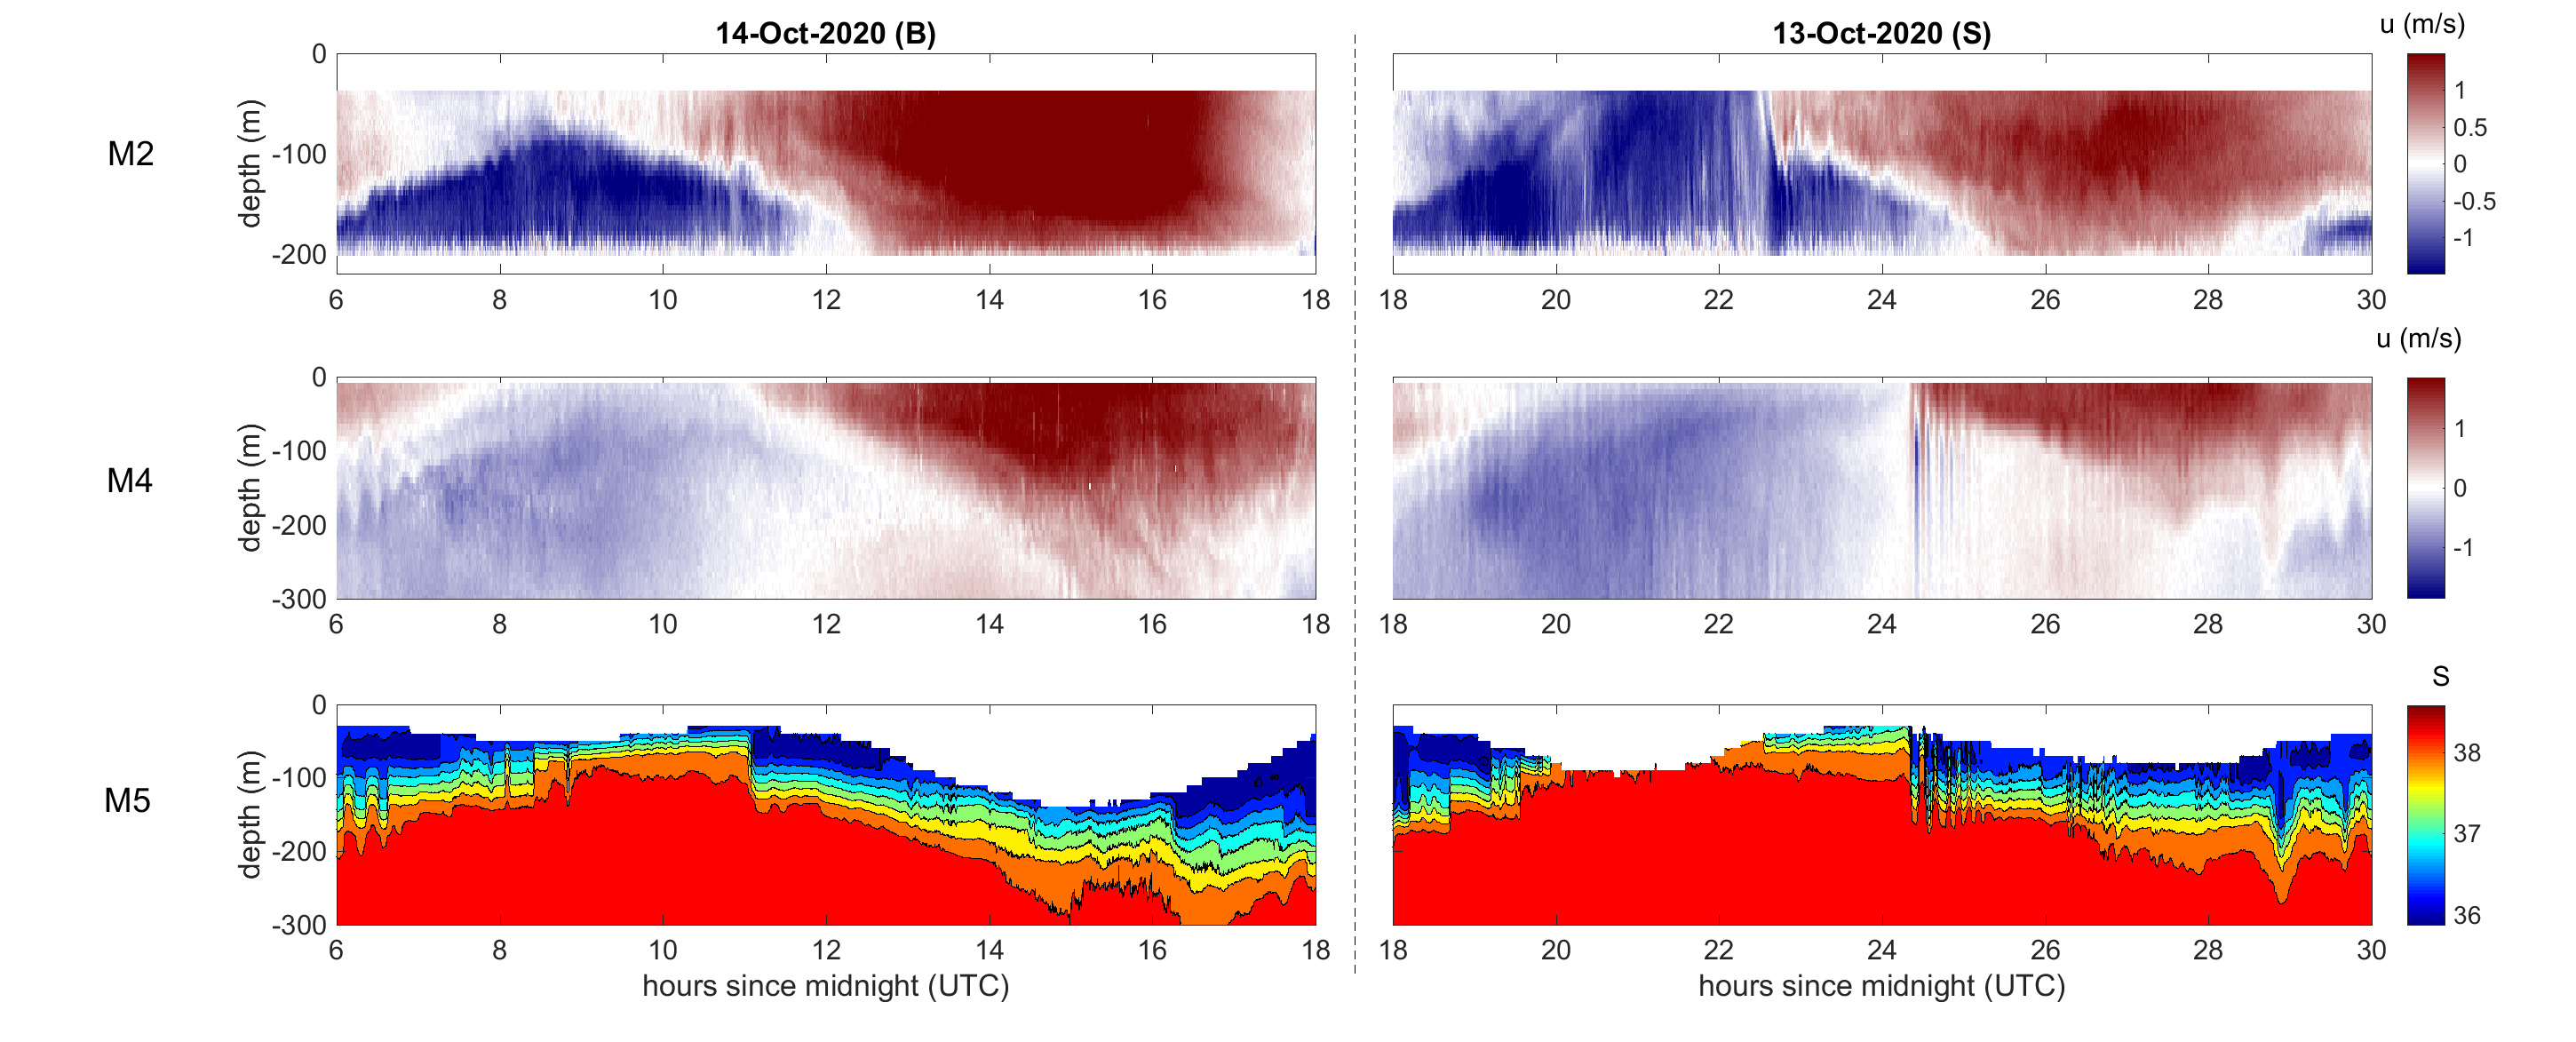
\includegraphics[width=\textwidth]{./GBR3D/US_moorings2.png}
 \caption {same as figure \ref{fig_moor_US1} for different time-periods.}
 \label{fig_moor_US2}
\end{figure}

\begin{figure}[!h]
% \centering
 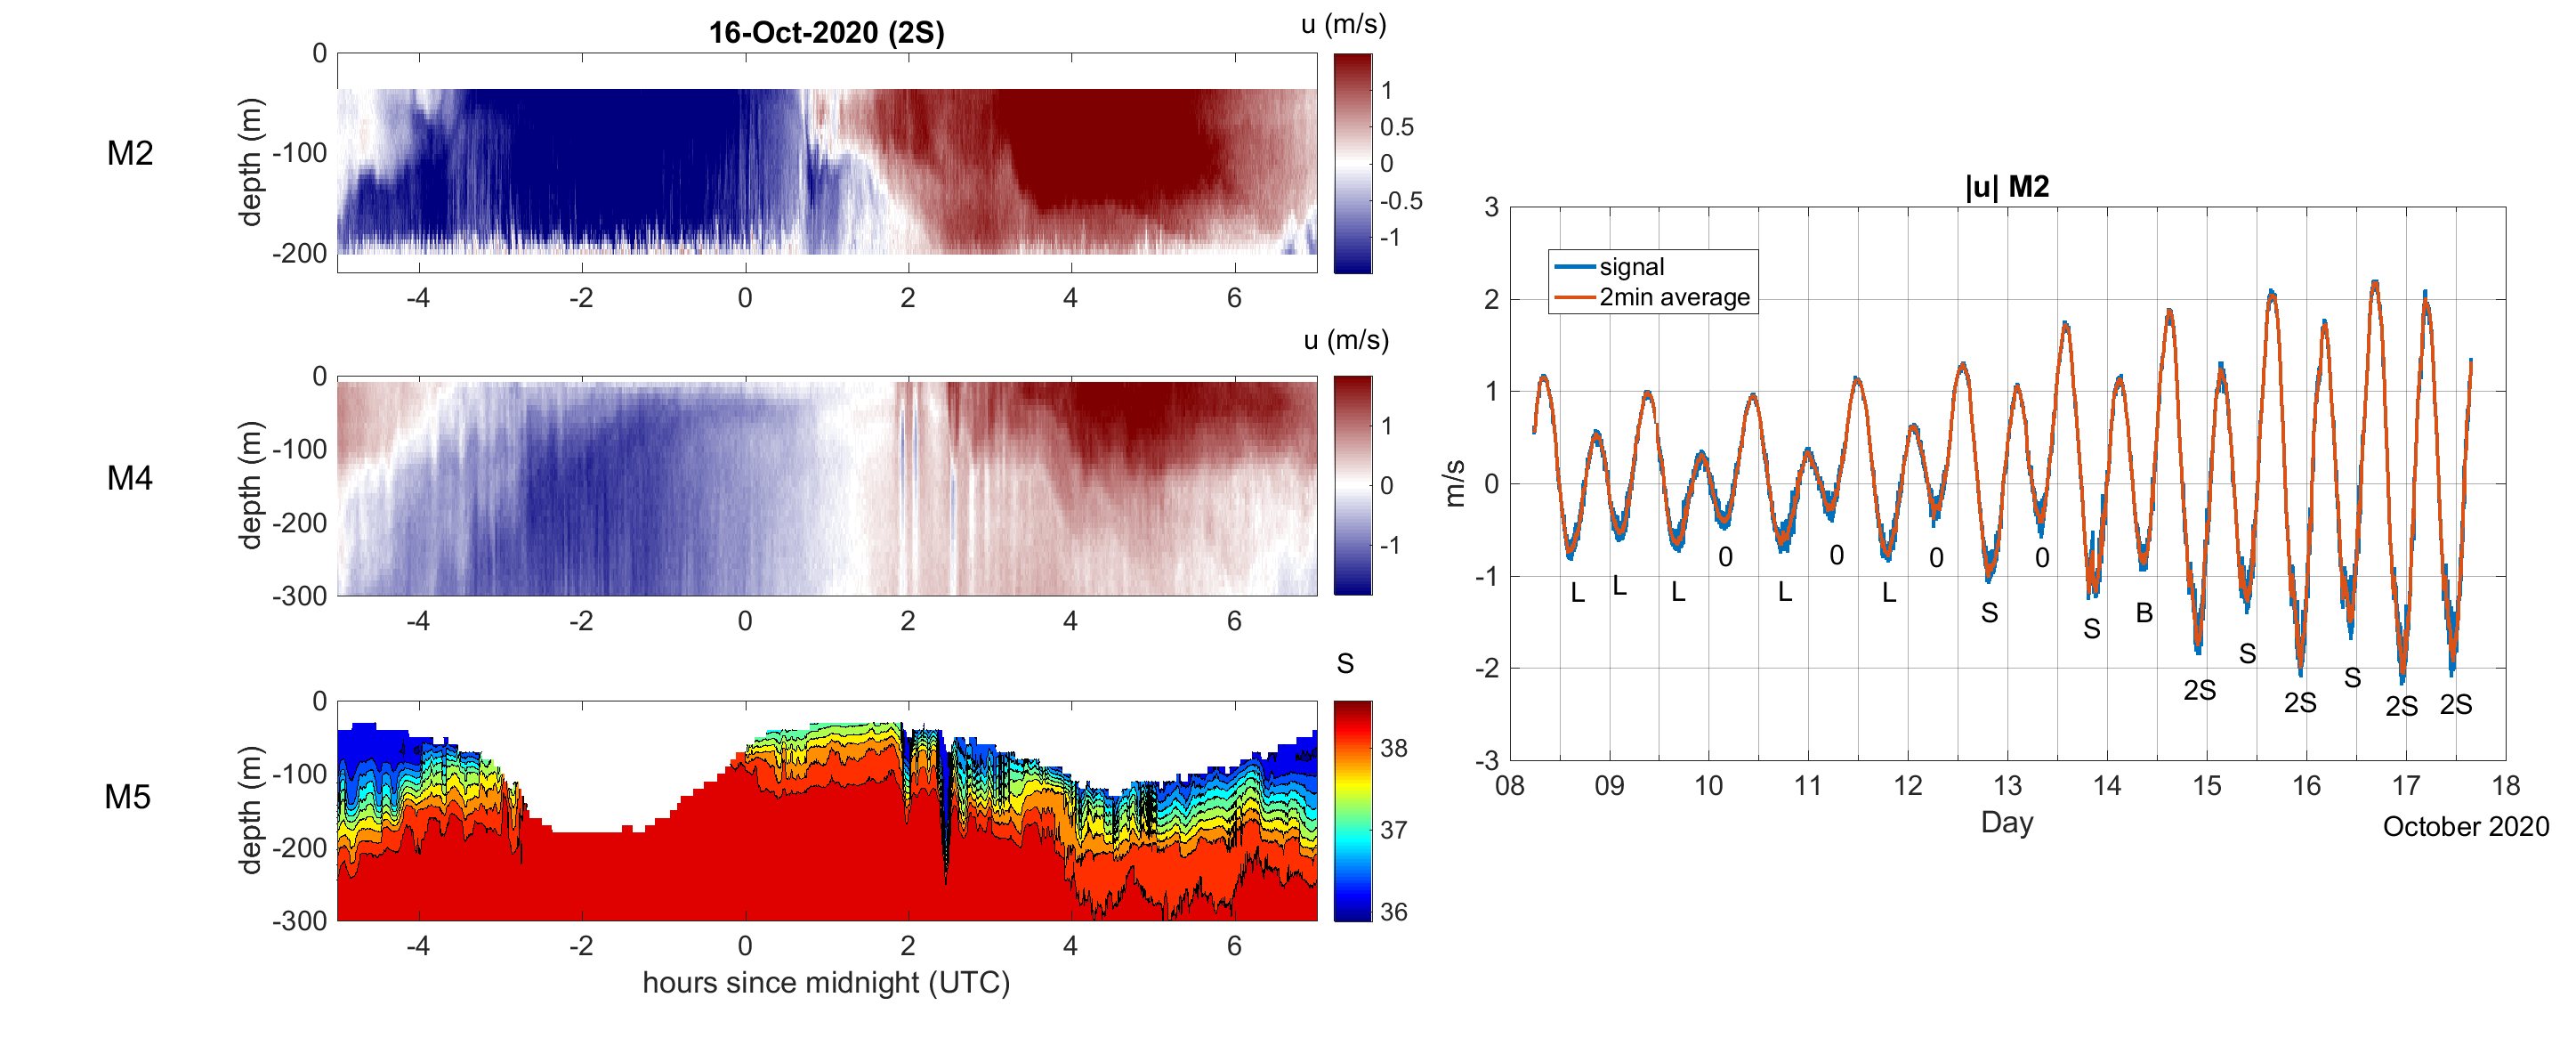
\includegraphics[width=\textwidth]{./GBR3D/US_moorings3.png}
 \caption {(A1 to A3) Same as figure \ref{fig_moor_US1} but for a different time-period. (B) Time-series of depth-averaged signal of the zonal component of currents from M2 data (in blue the instant signal recorded, in red the 2 minutes average). For each outflow is indicated the type of signal that is observed at M4 and M5 mooring (see text).}
 \label{fig_moor_US3}
\end{figure}

Figures \ref{fig_moor_US1} to (\noparref{fig_moor_US3}.a) present depth-time records of the zonal velocity (for M2 and M4 mooring) and salinity (for M5 mooring) for five different M2 tidal periods. Tilting by the strong currents provoked the depths of the CTD sensors of the M5 mooring to change overtime, sometime loosing the signal from tens to a hundred of meters at the top of the water column (for exemple see figure (\noparref{fig_moor_US2}.A3 at 15hUTC)). Additionnally, note that whereas the whole water column is presented in those figures for the M2 data, only the upper 300 m (of a 500-m-deep water column) are represented here for M4 and M5 data for a better visualization.

Similarly, figure \ref{Fig_moor_USs} presents the zonal velocity and salinity of the upper 300 m of simulated data at a grid point of coordinate (35.937°N;5.706°W), near M4 and M5, from the simulations SimNT (figures \noparref{Fig_moor_USs}A and B), SimIT (C) and SimST (D) of section \ref{sectionSim3D}. Although those simulations cover a different time-period, the simulated fields present similar patterns of internal waves traveling in the water column as the observed data.


\subsubsection{Currents at M2 and M4 mooring}

In the observations of currents made at mooring M2, periods of inflows and outflows can be distinguished respectively as having mostly eastward or westward components over the water column. During inflow periods, there are always at least two hours during which the whole flow measured by the captors is eastward (for example between 10 and 12 hours in figure (\noparref{fig_moor_US1}.A1)). During outflows, the current can be westward at all captors, as is the case in figure (\noparref{fig_moor_US2}.B1) and (\noparref{fig_moor_US3}.A1), but this is not necessarily the case. 

In figures (\noparref{fig_moor_US1}.A1) and (B1), for example, the baroclinic exchange structure of currents is still distinctive during outflows, with a weak eastward flow in the upper 120 m of the water column over a strong westward current. Figure (\noparref{fig_moor_US2}.A1) presents another case for which the flow in the upper water column becomes momentarily weakly westward between t = 7 h and t = 9 h, with a still clear shear interface at 100-m deep.

In the numerical simulations performed in section \ref{sectionSim3D}, an entirely westward flowing water column at M2 mooring corresponds to an area an hydraulic jump is present. In figure (\noparref{fig_moor}.A2), this location corresponds to the upflow area of the two types of hydraulic jumps identified in section \ref{sectionSim3D} (s-jump and w-jump), and depicted respectively as grey and black points.

At mooring M4, the flow of the water column can become unidirectional during both outflow and inflow periods during the spring tide part of the fortnightly cycle. In this occasions, a shear area still subsists that matches with the salinity interface between Mediterranean and Atlantic waters identified at mooring M5 (see for example at t = 14 h in figure (\noparref{fig_moor_US2}.A2) and (A3) at depth ranging between 150 and 200 m).

\subsubsection{Propagation of high frequency waves}

\begin{figure}[!h]
% \centering
 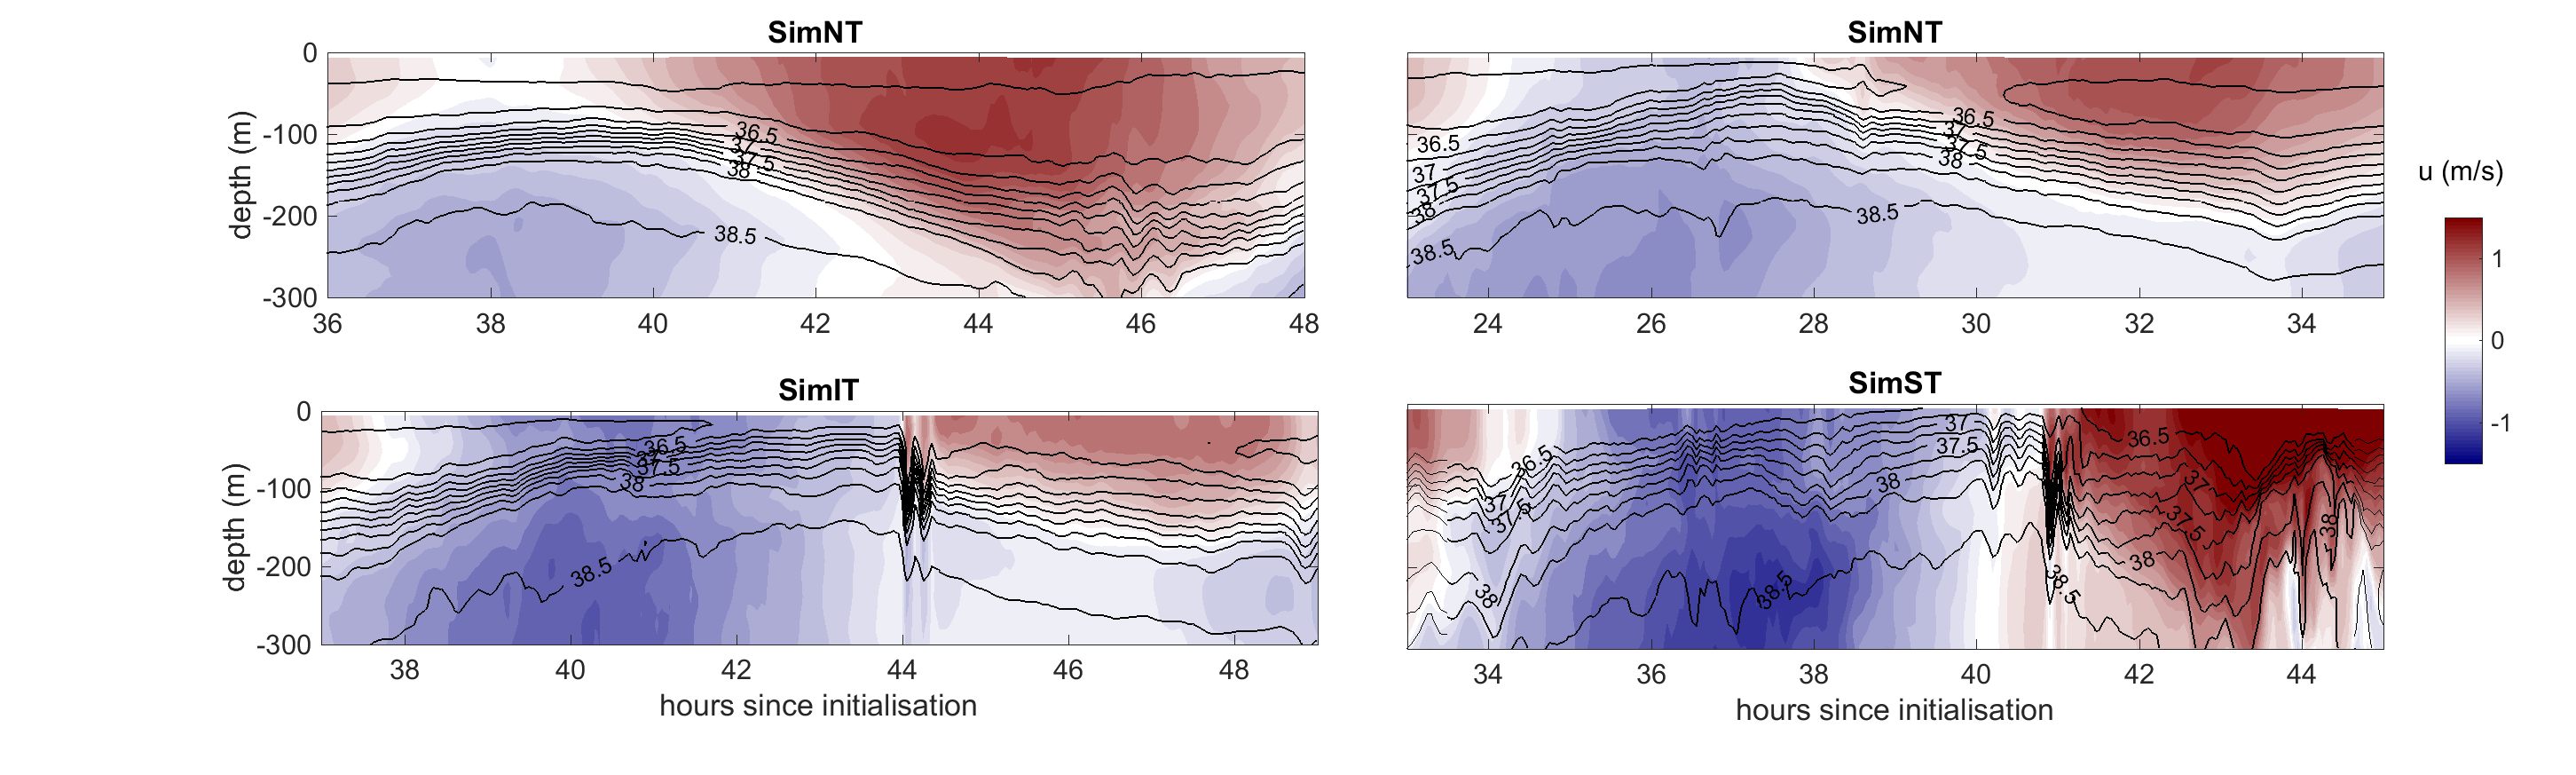
\includegraphics[width=\textwidth]{./GBR3D/US_M4SimMIV.png}
 \caption {time series of salinity (black lines) and zonal velocity (color) in the upper 300 m in simulations SimNT( A and B), SimIT (C) and SimST (D) of section \ref{sectionSim3D} at the gridpoint of coordinates (35.937°N;5.706°W). Abscises is simulation time. }
 \label{Fig_moor_USs}
\end{figure}

It is on the salinity interface observed at M5 mooring that the signal of propagating internal gravity waves can be spotted, sometimes matching with anomalies in the current field of mooring M4.

Figures (\noparref{fig_moor_US1}.B3) at t = 3 h, (\noparref{fig_moor_US2}.A3) at t = 8h30, and (\noparref{fig_moor_US2}.B3) at t = 19h30, show as a recurring feature an abrupt lifting of the interface, that does not appear in the simulations data of figure \ref{Fig_moor_USs}.

Another recurring signal in M5-mooring data are the large amplitude troughs that can be seen during the inflow period of the tidal cycle. In this data set, it appears clearly in observation data made at t = 29 h in figure (\noparref{fig_moor_US2}.B3). In simulation data (for example t = 49 h in figure (\noparref{Fig_moor_USs}.C)), this signal corresponds to a westward traveling train of ISWs that is generated by reflection off the Moroccan coast of the well-known eastward traveling ISWs train that is generated at CS.

The focus is now made on the signal showing up at M4 and M5 mooring, usually 3 hours or sooner after the maximal outflow at M2 mooring. Five distinctive types of signals are identified and categorized with letters o, L, B, S, and 2S :

\begin{itemize}
\item \underline{Linear-internal tide (o), figures (\noparref{fig_moor_US1}.A2-A3)}: the depth of the salinity interface at M5 mooring and maximum shear at M4 mooring evolves linearly, except for some low amplitude traveling waves at the interface in M5 mooring at t = 10h30. At M2 mooring (figure \noparref{fig_moor_US1}.a1), there is a distinctive shear in the water column during the preceding outflow, with slightly positive velocity in the upper layer. This signal is also seen in SimNT as shown in figure (\noparref{Fig_moor_USs}.A).
%
\item \underline{Small-amplitude internal wave (L), figures (\noparref{fig_moor_US1}.B2-B3)}: in the salinity data, there is a signal that looks like two internal waves of relatively small amplitude (10 m) at M5 mooring at t = 4h30. At M4 mooring, the depth of maximum shear of zonal velocity still evolves in a linear manner as in the previous (o) case. At M2 mooring (figure \noparref{fig_moor_US1}.b1), the interface of westward flow evolves at the same depth as in the (o) case but in the upper layer velocity becomes almost nil from t = 1 h to t = 3h30. This signal is also seen in SimNT in figure (\noparref{Fig_moor_USs}.B) at t = 28.5 h of simulation, and is associated there in the velocity field with a mode-1 anomaly.
%
\item \underline{Internal-traveling bore (B), figures (\noparref{fig_moor_US2}.A2-A3)}: at M5 mooring, the salinity interface drops by 50 m at t = 11 h which resembles the signal of a westward-propagating internal bore. At M4 mooring, however, the depth of maximum shear still evolves linearly, but before the arrival of the internal bore signal, the flow in the water column is negative at all depths. At M2 mooring over CS, the upper layer velocity is nil or lightly negative during the outflow. This type of signal is not recovered in the simulations that have been performed.
%
\item \underline{Train of internal-solitary waves (S), figures (\noparref{fig_moor_US2}.B2-B3)}: a succession of 7 troughs passes at M5 mooring starting at t = 24h15. The first one has an amplitude of 80 m. At M4 mooring, this series corresponds to mode-1 anomalies of the velocity field. At M2 mooring, the flow is westward throughout the water column during the preceding outflow, with an abrupt return to a sheared two-layer state at t = 22h30, corresponding to the loss of hydraulic control and the release of the western hydraulic jump over CS. In simulations, this type of signal is seen for instance in simIT and presented in figure (\noparref{Fig_moor_USs}.C) with two troughs at  t = 44 h. In these simulations, this type of signal at mooring M4 and M5 follows the release of a s-jump type of hydraulic jump (i.e., at maximum outflow, the western hydraulic jump is located over the shallowest part of CS).
%
\item \underline{Two close trains of internal-solitary waves (2S), figures (\noparref{fig_moor_US3}.A1-A2)}: five troughs can be seen propagating at M5 mooring starting at t = 2 h, but are not propagatingin order of decreasing amplitude. The first trough has an amplitude of 80 m and is followed by two short-wavelength, small-amplitude troughs. Then at t = 2h30, an over-100-m amplitude trough propagates at M5 mooring. It is in turn followed by a smaller-amplitude trough. The mode-1 anomaly of the velocity field is seen clearly at M4 mooring for the first two waves, then the fourth larger amplitude one. At M2 mooring, as in the previous (S) case, the flow through the water column transitions from wholly westward to sheared two-layer at t = 1 h. In numerical simulation SimST (figure \noparref{Fig_moor_USs}.D), four waves can be identified. They follow this pattern, the first two waves have decreasing amplitude, the third has a larger amplitude than the first two, and the fourth has a smaller amplitude. In this case, this pattern corresponds to two different trains of ISWs. The first (second) train corresponds to the previously  released hydraulic jump east (west) of CS. In the numerical simulations, this signal follows the release of a w-jump (i.e., at maximum outflow the west hydraulic jump is located over the western slope of CS).
\end{itemize}

Both S and 2S signals are linked to westward flow of the whole water column at CS, which should indicate that, as in the numerical simulations, a hydraulic jump was present west of M2 mooring.

The 2S case can be observed in numerical simulations and in figure (\noparref{Fig_moor_USs}.D). The amplitude of the first wave which corresponds to the eastern hydraulic jump of CS can however be very small. While the wave(s) produced by the release of the eastern hydraulic jump are always present, at the latitude of moorings M4 and M5, its amplitude depends (i) on the northern extent of the eastern hydraulic jump at maximum outflow (i.e., how high a latitude it reaches) and (ii) on the initial angle taken by the released non-linear wave as it first propagates in a slightly southern direction.

As the two sets of ISWs propagate further in the strait, the second train overtakes the first one. Indeed the propagation speed of ISWs depends on their amplitude (the larger the faster), so eventually they appear as a merged and sorted train of ISWs. For instance, the "S" structure in simulation appears because the wave released by the western hydraulic jump of CS overtook the eastern one(s) sooner due to their initial closeness.

So although it appears here that two cases are distinct (the S case following an s-jump and the 2S case following a w-jump), there might be a possibility that slowly propagating waves from an s-jump could also appear as a 2S structure at M4 and M5 mooring, and conclusion cannot be reached on the structure of the two hydraulic jumps at CS only on the basis of the signal at M4 and M5 moorings.


\subsection{Transition between outflow types \& ISWs generation in Gibraltar strait}

The classification of the previous section is applied to signals at M4 and M5 mooring following each outflow of the first observation period and is marked as annotations in figure (\noparref{fig_moor_US3}.B).

A pattern emerges linking outflow type and strength of the averaged currents at CS. The beginning of the period corresponds to the neap-tide part of the fortnightly cycle, and either (L) or (o) type of outflows are detected, with no hydraulic jump at CS. The first solitary wave is observed at M4 and M5 mooring the 12/10/2020. Due to the diurnal variation of the M2 tide, the tidal flow over the following period is weaker (less than 1 m/s) and the signal at M4 and M5 moorings is an (o) case.

Except for one specific (B) case (14/10/2020), during the remainder of the period, trains of ISWs (with either a S or 2S structure) are propagating through M4 and M5 mooring. The stronger outflows lead to (2S) signals in agreement with the numerical simulations presented in section \ref{sectionSim3D}. Under especially strong outflows, the internal hydraulic jump generated over CS is swept downstream as a w-jump, resulting in an initially increased distance between the eastern and western jumps. This distance may not be overcome as quickly upon release of the hydraulic jump as in the s-jump case. This explains the distinction between S and 2S cases, however as explained previously, for some outflows, the distinction between the two may remain subjective.

Only one (B) case is observed, it was not featured in numerical simulations so it is less evident whether it can be attributed to the presence of an hydraulic jump over CS. Whereas the variation with depth of currents at M2-mooring site in the preceding outflow shows a shallower interface and more westward currents in the upper layer than for the (o) and (L) cases, it may be more akin to a near supercritical flow regime engendering some form of propagating steepening interfacial disturbance.

It was seen in section \ref{section_sim3D_ISW} that, in numerical simulations, even if no hydraulic jump occurs at CS, the flow of the barotropic tide in the strait of Gibraltar can lead to the steepening of a long interfacial wave that later develops into a train of ISWs. This train contains a lesser number of ISWs than in the release of hydraulic jump case as it propagates toward the Alboran Sea. 

Figure (\noparref{fig_SAROBS}) is a SAR image taken during the Gibraltar 2020 campaign in the morning of October, 9. A curved surface signature of higher reflectivity can be seen in the Alboran Sea, looking like the front of an ISW (for exemple in figure (\noparref{fig_SARIES}.A)). But looking at (\noparref{fig_moor_US3}.B), all preceding outflows are of the "L" case for the signal at M4 and M5 mooring at this date, with no hydraulic jump at CS. The small amplitude internal gravity wave that was observed at M5 mooring, if propagating east, could be responsible for the signal in the Alboran Sea that looks like oe ISW, and is similar to what was encountered in simulations.

\begin{figure}[!h]
% \centering
 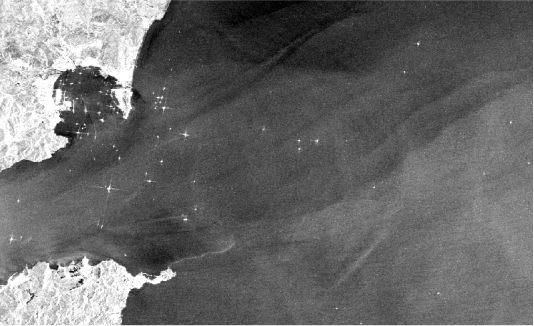
\includegraphics[width=0.6\textwidth]{./GBR3D/SAR_OBS_GEPETO.png}
 \caption {Sentinel-1 Synthetic Aperture Radar (SAR) image from 09/10/2020 - 6h18am UTC.}
 \label{fig_SAROBS}
\end{figure}


\subsection{Discussion \& perspectives}

A first confrontation between LES and observations has been carried out showing at least a qualitative agreement. Simililarities are found between simulated fields and four of the five types of signals encountered in data of moorings M4 and M5. Two of those signals, S and 2S are of clear trains of ISWs propagating after the release of the hydraulic jumps at Camarinal Sill that induces a westward flow in all the water column in M2 mooring data. 

For the L signal, the presence of the hydraulic jump is doubtful, but figure (\noparref{fig_SAROBS}) provides one satellite image of what appears to be as lone ISW signal propagating in the Alboran Sea after such an outflow. According to this observation, and the reproduction of this behaviour in numerical simulations, it is possible that the mechanism of release of the hydraulic jump is not the only one responsible for generation of the observed ISWs in the Strait of Gibraltar and in the western part of the Alboran Sea. ISWs trains are indeed observed in other areas of the global ocean, without being linked to the establishment andrelease of an hydraulic jump (see for exemple \citet{chen_2017}).

Looking at the barotropic currents measured at M2, there is a pattern linking the amplitude of the tide to the signal seen at the M4 and M5 moorings. Especially there seems to be a treshold over which hydraulic jumps and solitary waves begin to be observed. The reproduction of this treshold in numerical simulations of the Strait of Gibraltar is expected to be difficult. Even in high-resolution regional modelling such as in section \ref{sectionSim3D}, numerical parameters will influence the transition from a no hydraulic jump regimen to a generation of hydraulic jump one. The state of the stratification, for exemple, will play a part as the condition for Atlantic and Mediterranean layers to be supercritical, and hence on the moment hydraulic jumps begin to appear. This will depend on the quality of the water masses defined in the numerical simulation as well as atmospheric and large-scale forcings. Other important physical factors are the high-sensivity to the bathyetric data and the tidal forcing.

Several improvements have already been made over the simulations of section \ref{sectionSim3D}, but are still beeing evaluated and, as a consequence, have not been included in the present section. 
\begin{itemize}
\item Atmospheric fluxes are specified at the surface of the ocean.  This provides a better representation of the stratification in the upper surface and has important consequences on the characteristics of the pycnocline and thus on the characteristics of the internal waves, bores and solitons.
\item The high-resolution dynamics in the Strait of Gibraltar can now be explicitly simulated by downscalling the regional circulation (from the Gulf of Cadix to midway of the Alboran Sea). A three-step embedding has already been carried out using AGRIF library from 900-m to 60-m resolution simulations through a 180-m resolution implementation.
\end{itemize}
 


\section{Conclusion}

\color{green} Rappel méthode, bilan développement LES, bilan maquette...\color{black}




\section{Annexe : Singular Value Decomposition (SVD)}
\label{annexeSVD}
Singular Value Decomposition (SVD) consists in finding a basis of singular values and orthonormal singular vectors for a G x T matrix A (complex or real), so that :
\begin{equation}
A = U \Sigma V^* 
\end{equation}
Where the G x k matrix $U$ and k x T matrix $V$ (and its conjugate $V^*$) are the left and right singular vectors respectively, and $\Sigma$ is the diagonal k x k matrix of singular values associated to each couple of singular vectors.

To analyze a time-varryinig signal of variable $\psi$ on a 3D grid (or 2D as in section ..), the spatial field of each of the T timestep is appended into one column of length G to create the GxT matrix A, where T are the number of iterations of the 3D field. 

After proceeding with the SVD of this matrix A, the column number i of U is reformed into a 3D field that gives the spatial structure of the field of $\psi$ associated with the i singular value, that has a time-variation in the i row of the singular right vector V.

In section \ref{sectionSim2D}, SVD was applied to the complex field of $\psi=w+iu$. consecutive vectors of the basis with close singular value and that exhibited similar time-variations were combined to ... .In section \ref{sectionSim3D}, SVD is applied to the field of the real quantity $Q$.



\chapter{BPE}
\begin{itemize}
\item Résumé en français
\item papier
\end{itemize}

\chapter*{Discussion Conclusion}

\chapter*{Annexes}


\listoffigures

\listoftables

%%%%%%%%%%%%%%%%%%%%%%%%%%%%%%%%%%%%%%%%%%%%%%%%%%%%%%%%%%%%%%%%%%%%%%%%%%%%%
%              Bibliography
%%%%%%%%%%%%%%%%%%%%%%%%%%%%%%%%%%%%%%%%%%%%%%%%%%%%%%%%%%%%%%%%%%%%%%%%%%%%%
\bibliographystyle{apalike}
\bibliography{mybib}

%%%%%%%%%%%%%%%%%%%%%%%%%%%%%%%%%%%%%%%%%%%%%%%%%%%%%%%%%%%%%%%%%%%%%%%%%%%%%
\end{document}
%%%%%%%%%%%%%%%%%%%%%%%%%%%%%%%%%%%%%%%%%%%%%%%%%%%%%%%%%%%%%%%%%%%%%%%%%%%%%


%\newpage
%%%% En mettant PDF
%%%mettre autre pdf avec figure incluse aux bons endroits etc...
\addtocounter{section}{1}
\addcontentsline{toc}{section}{\protect\numberline{\thesection}Papier 2D}
%\includepdf[pages=-]{./GBR2D/PDF_GBR2D.pdf}%%!!attention decommenter package



\section{ccl français}
\begin{itemize}
\item Limitation de la simulations 2D, transition partie 3D
\end{itemize}


%%%%%%%%%%%%%%%%%%%%%%%%%%%%%%%%%%%%%%%%%%%%%%%%%%%%%%%%%%

\chapter{GBR3D}



%%\selectlanguage{english}
\hypersetup{pdfborder=0 0 0}
%\vspace{10\baselineskip}


%\selectlanguage{french}


\section{Resume français}




%-------------------------------------------------------------------------------------
\section{Papier 3D}
\subsection{Introduction}

The Atlantic - Mediterranean exchange occurring in the Strait of Gibraltar has been explained summarily in previous part (2D). It consists in Med waters exiting the Strait at depth as what has been dubbed the 'Mediterranean outflow' while Atl waters enter the Mediterranean basin at the surface.

Those Atlantic waters entering at the Strait are the principal contribution to the Mediterranean inflowing water budget, with the average transport of Atl waters at Gib being of the order of 1Sv. The net exchange itself is of the order of 0.1Sv as a positive entry that offsets the otherwise net evaporation occurring on the integrated surface of the Mediterranean basin \citep{bryden_1994}.
Since the Med basin is otherwise a closed basin, the Mediterranean waters exiting the Strait of Gibraltar are the result of the transformations into intermediate and deep water masses of the Atl waters that circulated in the Mediterranean.
More details are provided in this section on the characteristics of the Strait, the exchange and its variability and the processes that take place during it.






\subsubsection{Circulation in neighbouring areas (Cadix and Alboran)}

(de Pascual-Collar ; NAjanro 2012 ; Sanchez Garrido 2013 ;Lorente 2019 ; garcia lafuente 2017)


\textit{Atlantic side}

The surface waters that end up entering the Strait are NACW and SAW\citep{millot_2014,naranjo_2015}. They are carried by the Portugal and Azores Current into Gib as part of the eastern branch of the north atlantic subtropical gyre \citep{barton_2001}

Below this surface circulation, can find in the Northern Atlantic the med outflow/the mediterranean watermass that was transported out of the Strait by the MEditerreanaen outflow. It first flows in the Gulf of Cadix, rotating to north due to geostrophy and flowing along the bathymetry of the continental slope\citep{price_1993,gasser_2017} and west of the Gulf of Cadiz stabilizes to its neutral buoyancy level at 1000m depth as the Mediteranean water mass\citep{price_1993}. Meddies, salty lenses of water with negative (?) vorticity able to 'survive' for years that are encountered in the open ocean, are generated along the canyons and caps encountered by the Mediterranean outflow in the Gulf of Cadiz \citep{bashmachnikov_2015}. The Mediterranean outflow itself participates in the global circulation/north atlantic overturning circulation(?) by salinification of the overall north atlantic basin with the spreading of the mediterranean water mass in the open ocean and decaying of meddies, but also with a part of the outflow directly joining circulation at the pole \citep{price_1993,jia_2007}.


\textit{Mediterranean side}


Surface waters exiting the Strait at the east enter the Alboran Sea as the Atlantic Jet (AJ). The circulation of the Alboran Sea is variable, with the most common state having two anticyclonic gyre (WestarnAlboranGyre ans EasternAlboranGyre), but not uncommon that only one of the two is present \citep{millot_2005}. The WAG is coupled to the Atlantic jet, that usually constitutes its northern branch, however variability of the AJ due to meteorological and tidal forcing can destabilize this system \citep{sanchez-garrido_2013,lorente_2019}.

At depth, several mediterranean water masses enter the strait. In the Alboran Sea, identified are LIW (for Leventine Intermediate Water) and WMDW(West MEditerranean Deep Water), with other water masses of the western med bassin like TDW (Thryenian Deep Water) also being detected (maybe)(Millot). There is a south/north repatition of those watermasses, with TDW, LIW and other intermediate waters more abundant in northern part of Alboran sea, and WMDW flowing more in south part \citep{millot_2014}. As the depth from teh Alboran to the Strait decreases, it is more difficult for the deeper WMDW to enter the strait, and the flow can be regulated by mechanisms such as the strength of the WAG or the overall production of WMDW linked to winter convection (Najanro 2012).


\textit{Gen}

Whether look at inflowing (in reference to the med basin) Atl waters or outflowing (ditto) Med waters, they incorporate signature of respectively the med waters (Macias 2006) and atl waters (Millot 2006,GarciaLafuente2011). This is due to mixing occurring in the Strait, driven by small scale processes of varying strength. 


%%%%%%%%%%%%%%%%%%%%%%%%%%%%%%%%%%%%%%%%%%%%%%%%%%%%%%%%%%%%%%%%%%%%%%%%%%%%
\subsubsection{Morphologie et marée barotrope et masses d'eaux (et ajouter atm???)}
%%%%%%%%%%%%%%%%%%%%%%%%%%%%%%%%%%%%%%%%%%%%%%%%%%%%%%%%%%%%%%%%%%%%%%%%%%%%%


The Strait is inclined of 15$^\text{o}$ from the east direction. Away from continental plateau, Camarinal Sill is the shallowest point with depth averaging at 300m. Relative to Camarinal Sill, Strait is narrower but deeper on the east side. On the west side, shallower, with two troughs on each side of a submarine mount called Majuan Bank. The northern trough is shallower than the southern one, which also includes another sill, called Espartel Sill. Those two troughs are the two pathways the Med outflow take to join the Gulf of Cadix, with most of the flow taking the southern deeper path (18 \% au nord selon Soto-Navarro 2014)


The barotropic M2 semi-durnal tide from the North Atlantic is the foremost varying signal for the currents in the Strait, propagating from south to north with amplitude decreasing from west to east\citep{candela_1990}. During Flood (ebb) tide, barotropic currents ate westward(eastward). The Currents associated with the barotropic tide are same amplitude as the mean circulation, can reverse the flow of med and/or atl waters for certain sections(Sanchez Roman 2012), and have a pronounced neap-spring tide cycle.

Wind is funnelled through the strait and is either westward or eastward/principally zonal with speed can reach 25m/s(Candela 1989). Wind stress affects only the first tens of meters of circulation in the Strait (Candela 1989), which can be sufficient to affect the Atlantic Jet, either accelerating(and making it exit the Strait at various angle) or decelerating it(can even stop it)(Lorente2019). Otherwise, the integrated effect of atmospheric pressure over the Mediterranean basin influence the net flow through the Strait(Garcia Lafuente 2002).





%%%%%%%%%%%%%%%%%%%%%%%%%%%%%%%%
\subsubsection{Baroclinic Exchange and small scale processes}


The circulation of eastward Atlantic waters at the surface and westward Mediterranean waters at depth sets up a baroclinic exchange in the Strait of Gibraltar. Due to amplitude of the barotropic currents, it is intermittent with regard to the M2 tide. One can thus see the exchange as a Reynolds(?) decomposition of an average with tidal contribution as eddy-fluxes that impacts secondary characteristics of the exchange (Naranjo 2014, etc..), and which have a more important amplitude at CS (Vargas2006).  

The exchange varies with other greater timescales than the semi-diurnal tide, with the lower frenquencies (seasonal,interannual) usually linked to atmospheric forcing over the Mediterranean (SanchezRoman2012?). But the tidal eddy-fluxes have their own variability linked to the spring-tide cycle and monthly tide, with for example a greater depth and stronger shear during neap tides, but more intense mixing in spring tide (Naranjo 2014, Vargas 2006).

Behind those characteristics varying at the tidal time-scale are small scale processes occurring in the Strait of Gibraltar.



Firstly, due to the limited horizontal and vertical extent of the Strait that channels the superposed average exchange flow and barotropic tidal currents, the flow in the Strait can become supercritical in regard to internal gravity wave propagation. East (west) of the Camarinal Sill the flow in atl (resp. med) layer will become supercritical, although the detail of how regular/their disposition and geometrical extent depends on the framework one uses. (exemples: Farmi et Armer 1988,Sannino 2007,Sanchez Roman 2012,Vargas 2006...)In particular, hydraulic control occurs at Camarinal Sill episodically.

There, development of two hydraulic jump reflecting the geometry of teh sill and can be observed on satellite imagery (brandt1996).The hydraulic jump stays approximately 4 hours at CS during outflows(Vlasenko 2009) and is where intense mixing occurs (Wesson andGregg;Lafuente...2011,MAcias2006(?)), billows from Kelvin-Helmoltz type instability of the flow in the lee of the hydraulic jump and advected westward by med waters(Wesson andGregg). In addition Bruno 2013, the establishment of hydraulic jump brings chlorophyll-rich waters in the center of the Strait.

Then propagate as LAIWs (Large amplitude Internal waves) also called solitary waves (.Farmer and Armi 1988) due to balance between non-linear and non-hydrostatic dispersion. Have been observed at the surface, and at depth (Ziegenbein (1970), Watson and Robinson 1990,Farmer and Armi 1988,SanchezGarrido 2008,etc.). They transport some chlorophyll (Bruno2013) and expect to make remote mixing in Alboran Sea.

ISW are generated at each tide except when westward current are not strong enough for hydraulic criticality at for neap tide (Watson and Robinson 1990, Garcia Lafuente 2000). Refracted as it exits the Strait by interaction with its boundaries, either as a curve or asymmetrically with an angle in the north(Watson and Robinson 1990).

The hydraulic jump and generation process can be achieved in numerical simulation by hydrostatic models but need non-hydrostatic one for propagation (Brandt 1996 ; (Vlasenko 2009)).



%%%%%%%%%%%%%%%%%%%%%%%%%%%%%%%%%%%%%%%%%%%%%%
\subsubsection{Impact, num et Plan}

Those small scale processes are responsible for the mixing of atl and med waters in the Strait, and the characteristics of the water masses involved in the baroclinic exchange at Gibraltar are not conserved(garcia lafuente 2017 : difficult to link characteristics at ES (INGRES, long term mooring to monitor outflow) to processes in the Mediterranean). The enhanced mixing in the Strait then has to be parametrized in coarsely resolved global/regional models the feedback to/in water mass composition that will impact circulation of the MEditerranean and North Atlantic. 


Following Hilt2020, here 3D sigma model,non-hydrostatic and decadal horizontal resolution that at least resolves the greater scales of mixing in the Strait. In particular focus of different tidal forcing case along a neap-spring tide cycle, how the flow characteristics and intensity of mixing processes is affected in simulation by this variability.


The numerical simulation framework constituted of three simulation periods is presented in section \ref{section3Dnum}, with various diagnosis that have been applied to said simulations /experiments then presented (blah) in section \ref{PartDiag3D} . Section \ref{section3DRes} presents results pertaining to the hydrological state of the flow depending on the strength of barotropic tidal currents, the propagation of ISW in the simulations, then areas of generation of primary instabilities, ending with a comparison of turbulence scheme.






\subsection{Numerical Configuration}
\label{section3Dnum}
\subsubsection{Numerical framework}

Simulations are run using CROCO-NBQ as was the case in Hilt 2020 (see a presentation of CROCO-NBQ there ... and in introduction of manuscript???) . Table \ref{tab_NH-HR} summarize some simulation choice. Otherwise, Non-linear equation of state, noslip condition at the bottom,etc...  The turbulent closure scheme used in all simulations except the ones of paragraph ... is Smagorinsky with coef chosen 0.05. For paragraph ... three simulations use Smago with coefs $10{-3}$,$10{-2}$,$10^{-1}$ , and one use GLSk-$\epsilon$.

Bathymetry data from 100m resolved MNT SHOM, smoothed for pressure gradient... is shown in figure \ref{FigBathy3D}. (bathy seuillée?)


Initialisation and open boundary conditions (that incude tdial forcing) are from a simulation of the operational Med and Black Sea ENEA using MitGCM (ENEA, Rome)\footnote{http://www.enea.it/it/seguici/pubblicazioni/pdf-volumi/cresco-report-2016.pdf}, whch serves as parent simulation. The parent simulation as an horizontal resolution in the strait of $\approx$ 700m and vertical z-levels (repartition?), that are interpolated on grid of horizontal resolution 45 m with 40 evenly spaced vertical $\sigma$-levels. As noted in table ..., this is sufficient to be more resolved in the vertical direction than in the horizontal for the whole simulation domain. At Camarinall Sill, vertical resolution varies from $\approx$7.5m at the top to $\approx$12.5m downslope. No atmospheric forcing is embedded in the simulation.

The first 6 hours of simulation are run in CROCO-Hydro at 50m resolution and the last field is used to restart in NBQ mode. Otherwise the balance in MitGCM is to coarse for stability at high resolution.

\begin{table}[!h]
        \centering
        \begin{tabular}{|p{\linewidth/3}|c|c|}
                \hline
                Grid Extension & \multicolumn{2}{c|} {6°4.8'W  5°3.4'W ;}\\
                & \multicolumn{2}{c|} {35°23.8'N  36°27.4'N}\\
                Number of horizontal grid points & \multicolumn{2}{c|} {2049x2621}  \\
                Number of vertical $\sigma$-levels & \multicolumn{2}{c|} {40} \\
                $\Delta x = \Delta y$ & \multicolumn{2}{c|} {45 m}\\
                Depth & Min & Max\\
                & 26 m & 960 m\\
                $\Delta$z & 0.7 m & 24 m\\
                Internal time-step ($\Delta t_s$) & \multicolumn{2}{c|} {1 s}\\
                External time-step ($\Delta t_f$) & \multicolumn{2}{c|} {1/11 s(change 1/14)}\\
                Advection scheme & \multicolumn{2}{c|} {WENO-5} \\
                Viscosity $\nu$ & \multicolumn{2}{c|} {10$^{-6}$ m$^2$/s} \\
                Diffusivity $K_\rho$(aussi Ks et Kt) & \multicolumn{2}{c|} {10$^{-6}$ m$^2$/s}\\
                Pressure/accoustic wave speed$C_s$ & \multicolumn{2}{c|} {400 m/s}\\
                Tidal harmonics (from ENEA) & \multicolumn{2}{c|} { $\text{M}_{\text{2}}$, $\text{S}_{\text{2}}$,$\text{K}_{\text{1}}$, $\text{O}_{\text{1}}$ }\\
                \hline
        \end{tabular}
        \captionof{table}{Simulation parameters}
        \label{tab_NH-HR}
\end{table}


\begin{table}[!h]
        \centering
        \begin{tabular}{|c|c|}
                \hline
                Closure scheme & Simulation name\\
                \hline
                Smago 0.005 & SimIT,SimNT,SimST\\
                Smago 0.001 & SimIT-S001\\
                Smago 0.01 & SimIT-S01\\
                Smago 0.1 & SimIT-S1\\
                GLS K-$\epsilon$ & SimIT-Kep\\
                \hline
        \end{tabular}
        \captionof{table}{Simulation names (ou combiner avec tableau d'avant ???)}
        \label{tab_sim3Dnames}
\end{table}


\subsubsection{Tidal forcing and simulation period}
The tidal forcing is integrated to the boundary forcing by the parent simulation. As indicated in table \ref{tab_NH-HR},  it comprises four tidal harmonics (?)($\text{M}_{\text{2}}$, $\text{S}_{\text{2}}$, $\text{K}_{\text{1}}$, $\text{O}_{\text{1}}$). Due to computational cost constraints, simulations are run for 3 days along 3 different periods of September of year 2017 (close to equinox). The date of the beginning and end of each NBQ simulation is surmised in table \ref{tab_dates_MIV}, and does not include the 6hour hydrostatic spin up period. The comparison of the sea-level anomaly between a grid point near Tarifa (coord -5.6° - 36.01°) in both the parent MitGCM and CROCO simulation and the tidal gauge data (from Puertos del Estado) are shown in figure \ref{fig_maree_tar}. Can see close to the parent simulation except in the neap tide period.

\begin{table}[h]
        %\begin{minipage}{.6\textwidth}
        \centering
        \begin{tabular}{|c|c|c|}
                \hline
                Situation & Simulation name & Dates (UTC)\\
                \hline
                Intermediate Tide & SimIT & 10/09/2017 19h00 - 13/09/17 01h00  \\
                Neap Tide& SimNT & 13/09/2017 16h00 - 15/09/17 17h00 \\
                %\hline
                Spring Tide& SimST & 19/09/2017 22h00 - 21/09/17 23h00  \\
                \hline
        \end{tabular}
        \captionof{table}{Périodes de simulation pour les 3 sitituations VE, MM et ME}
        \label{tab_dates_MIV}
        %\end{minipage}
\end{table}

\begin{figure}[!h]
        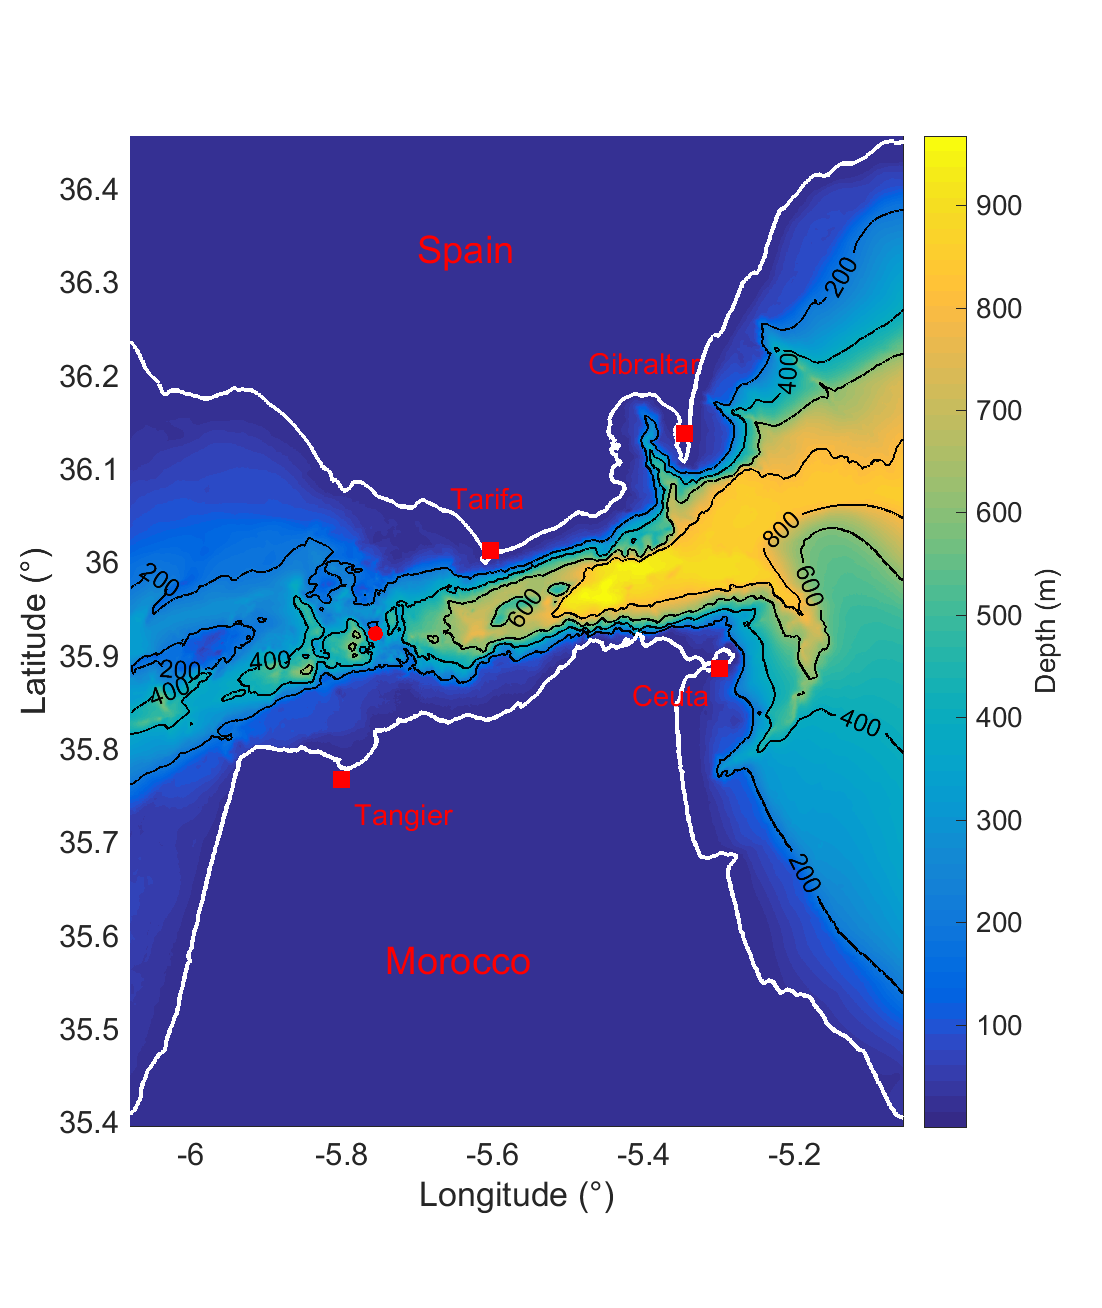
\includegraphics[width=0.5\textwidth]{./GBR3D/FigBathyVHR.png}
        \caption{Area and Bathymetry used for the simulations. The red dot denotes the point at Camarinal Sill where the zonal barotropic current is taken as reference in following figures.!!!Changer en anglais tangIer}
        \label{FigBathy3D}
\end{figure}



\begin{figure}[!h]
        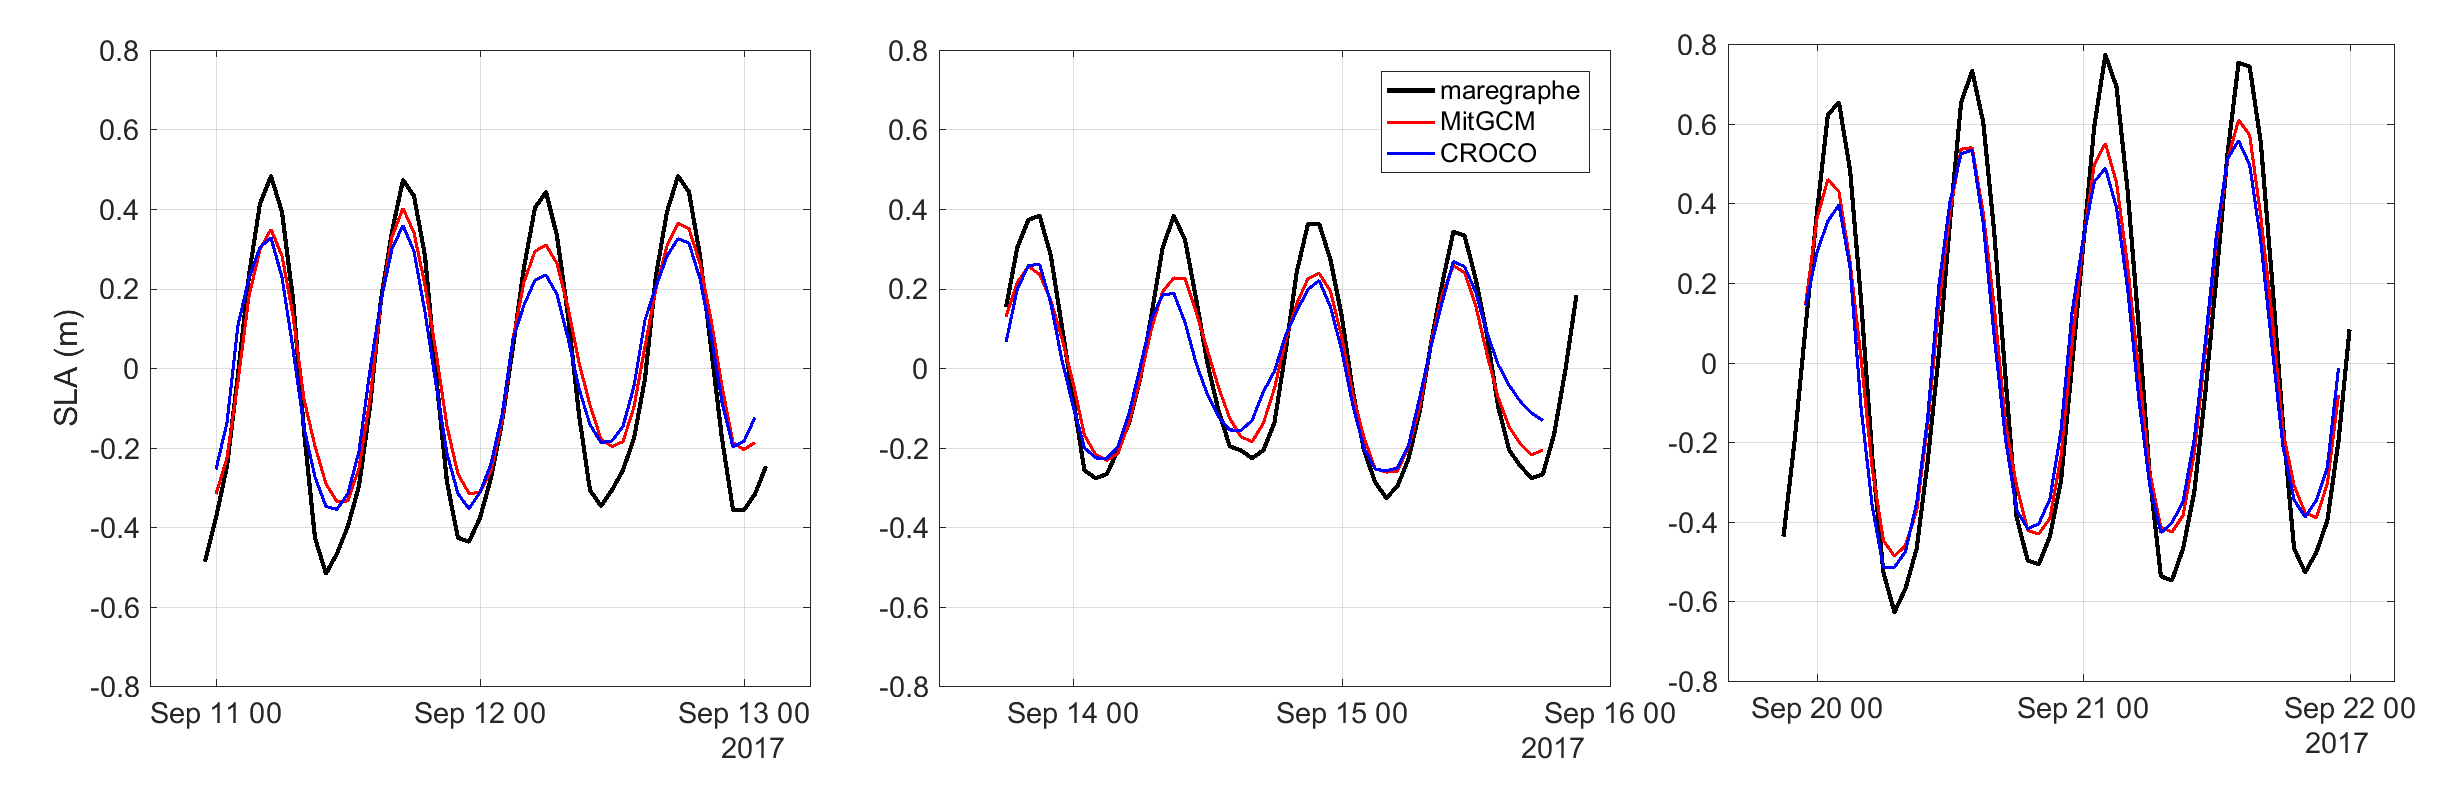
\includegraphics[width=\textwidth]{./GBR3D/SLA_Tarifa_ME2VE2IES.png}
        \caption{Sea level-anomaly at Tarifa from tidal gauge data (black) or at the nearest grid point for parent simulation (red) and CROCO simulation (blue), for situation ME (a), MM (b) et VE (c)}
        \label{fig_maree_tar}
\end{figure}

\subsubsection{Water masses}


\begin{figure}[!h]
        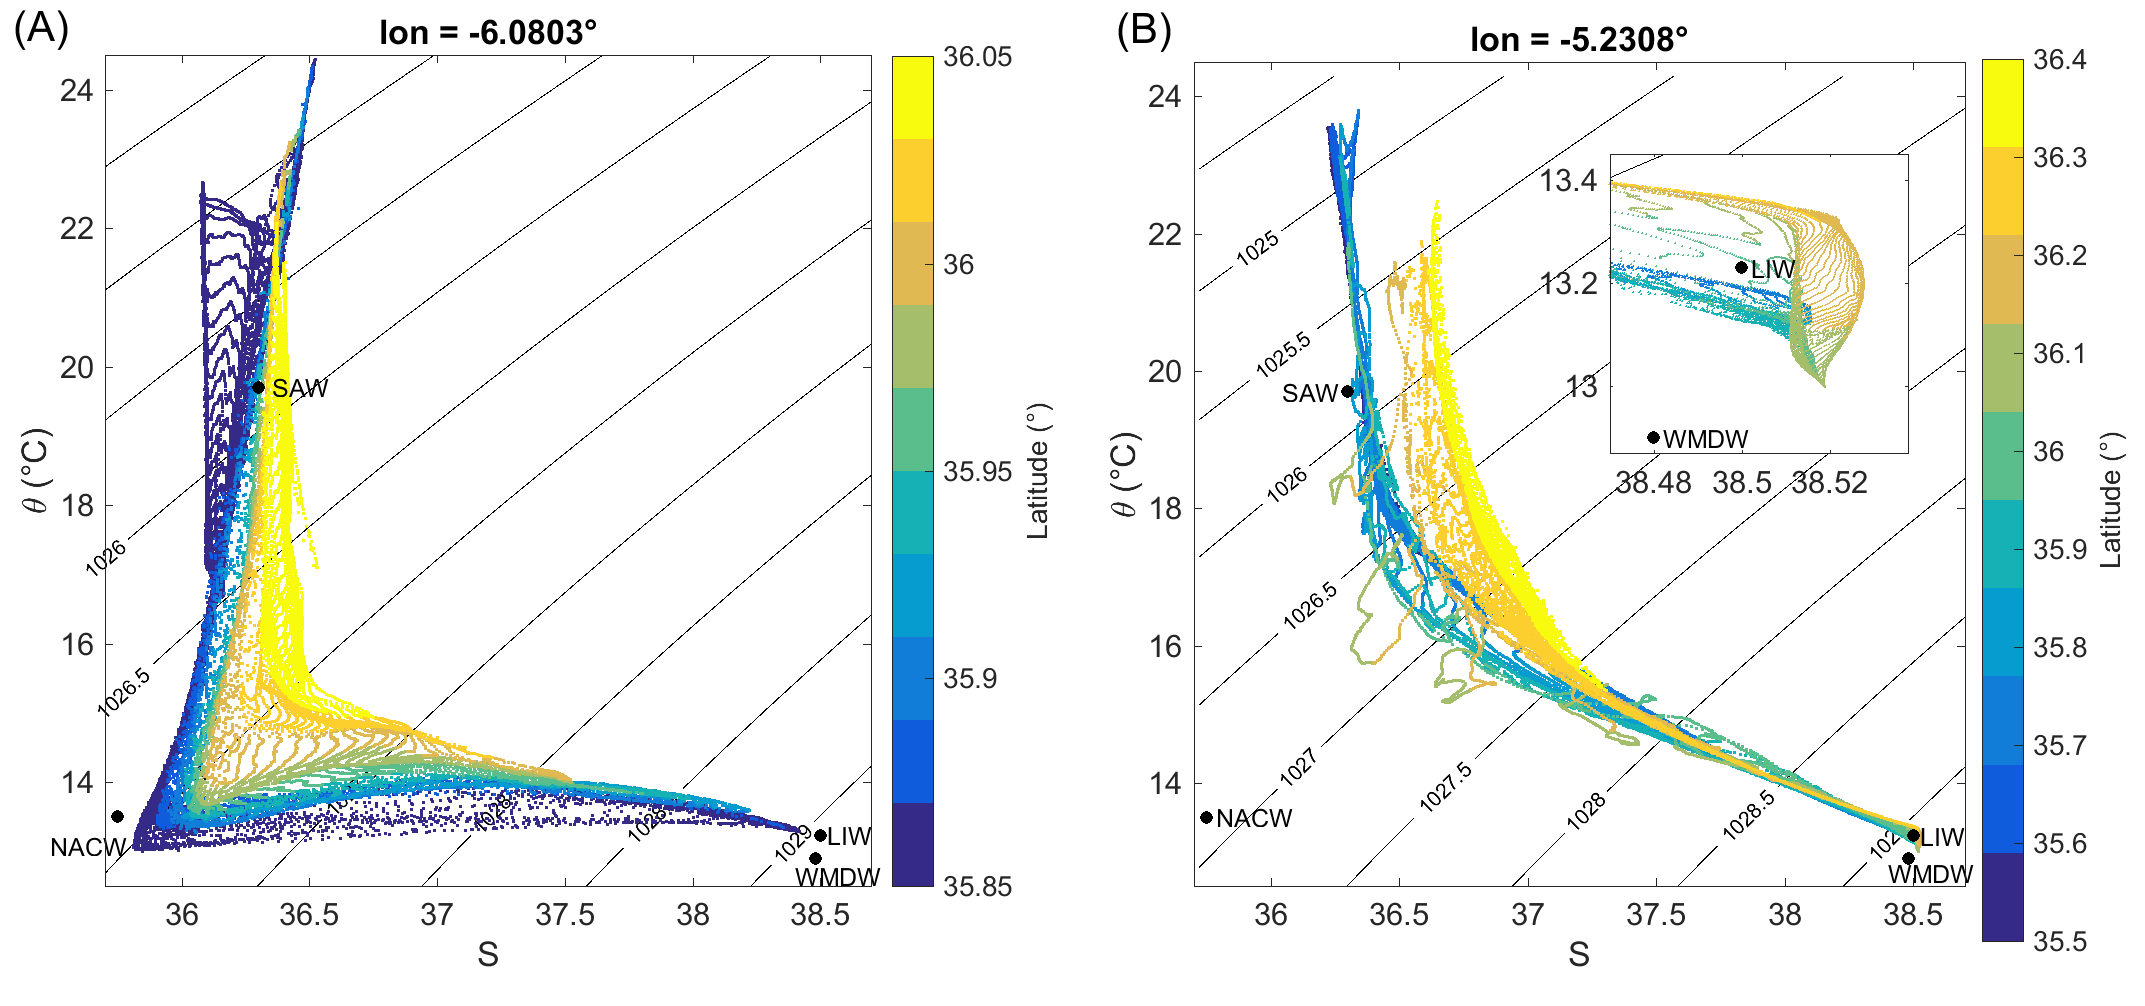
\includegraphics[width=\textwidth]{./GBR3D/WM_ini_IES.png}
        \caption{$\Theta$-S diagrams of grid points at 6.08$^\text{o}$W (a) and 5.23$^\text{o}$W in first timestep of SimIT, color indicates the latitude of each grid point. Are indicated cenroid definition of certain water masses according to Najanro2014}
        \label{Fig_Ini_WM3D}
\end{figure}


Figure \ref{Fig_Ini_WM3D} shows the $\theta$-S diagrams for east and west entry of the Strait in initial tracer field of simulation SimIT. As expected, for med waters see on the west side two signals for the two pathways of the med outflow, on the east side see distinctly a deep water mass and an intermediate one that could be interpreted as analogous to WMDW and LIW, with the latter being present mostly on the northern part, however in the simulation saltier and warmer waters than expected in bibliography. For atl waters, NACW present on west of domain, less on east. On east side, see difference surface water north/south of the opening of the Strait, with saltier surface waters in the north.




\subsection{Numerical diagnosis}
\label{PartDiag3D}

\subsubsection{Interface definition}

The analysis of simulation result is based on two layer definition of an Atlantic waters layer and Mediterranean waters layer. They are defined in regard to a reference salinity, with the interface defined as the height of the first water parcel from the top down in the water column for which salinity is above the reference salinity.

The reference salinity is taken as varying along the Strait as a hyperbolic tangent function of longitude centered at the Camarinal Sill to account for the different water mass composition in the eastern and western part of the Strait of Gibraltar. 

\begin{equation}
	S_i(x)=tanh(\frac{x-X_{CS}}{DX})\frac{S_M-S_m}{2}+\frac{S_M+S_m}{2}
\end{equation}
with $X_{CS}=5.75^o$, $dx=0.25^o$, the location and width of the Camarinal Sill in degrees, $S_M=37.39$ and $S_m=37.1$ the max and minimum values taken respectively east and west of the sill.

%This may not give the perfect interface at any given time...

\subsubsection{Froude layer number}

With the atlantic and mediterranean layers defined as above, the Froude layer number for internal gravity wave is computed at each 2D grid point as : 

\begin{equation}
F_i=\frac{U_i^2}{g'h_i} , \ \text{with} g'=g \frac{\rho_2-\rho_1}{\rho_0}
\end{equation}

where $\rho_i$ averaged density in layer i,  $U$ is averaged velocity norm over the layer i of height h. If $F_i>1$ say that the flow in layer i is supercritical.


\subsubsection{Hydraulic Jump detection, acceleration of flow}

\begin{figure}[!h]
 \centering
 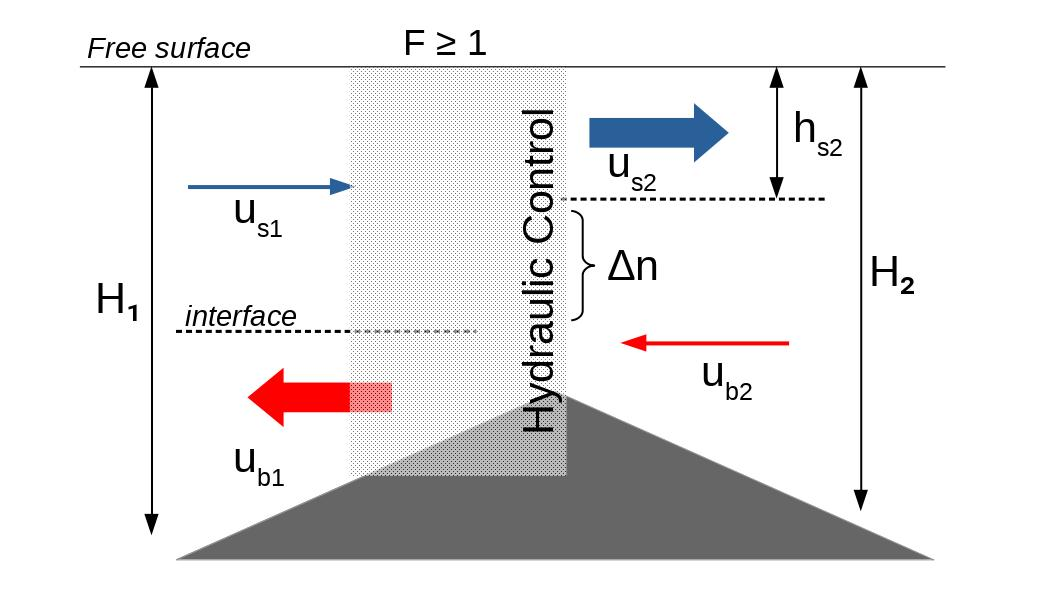
\includegraphics[width=0.5\textwidth]{./GBR3D/schema_diagressaut.jpg}
 \caption {Schematic of flow upstrean and downstream of hydraulic jump at Camarinal Sill, Strait of Gibraltar}
  \label{schemaRH}
\end{figure}


A simple diagnosis for detection of the hydraulic jump at Camarinal Sill in the simulations is based on the impact such a structure has on the flow. As shown/schematized/sketched(?) in figure \ref{schemaRH}, hydraulic jump (also called hydraulic drop) induces a drop of the interface depth. Since the flow in the Strait is canalised by bathymetry (for med flow) and coast (for atl flow), there must be conservation of flux from one section downflow and upflow of the hydraulic jump, which with the variation of the interface depth, means acceleration/deceleration of flow (depending on which layer is reference).

The drop in interface depth is noted $\Delta n=b_2-b_1$, the variation of bottom depth $\Delta H=H_2-H_1$ and the acceleration in the bottom layer $\Delta u_b = u_2-u_1$. For the bottom layer conservation of flux is :
\begin{subequations}
\begin{alignat}{2}
  \displaystyle
&u_1 (H_1-b_1)&& = u_2 (H_2-b_2)\\
& &&= u_1 (\Delta H + \Delta n) + u_1 (H_1-b_1) + \Delta u_b (H_2-b_2)
\end{alignat}
\end{subequations}

\begin{equation}
\Delta u_b = -u_1 \frac{\Delta H + \Delta n}{H_2-b_2}
\end{equation}

For the surface flow, similarly can find
\begin{equation}
\Delta u_s = - u_1\frac{\Delta n}{b_2}
\end{equation}

Velocity in the area of the hydraulic jump must validate condition of (at least) critical flow, ie Froude number $\geq$ 1. We search minimal condition for hydraulic jump so $F=1$, or $U=c$, taht is the flow ceerity equals the phase speed of internal wave. If for the latter we take the definition of interfacial speed can have an expression for $u_1$: 
\begin{equation}
|u_1|=c=\sqrt{g' \frac{(H_1-\Delta n - b_2)(\Delta n + b_2)}{H_1}}
\end{equation}



In the end, some parameters are chosen as threshold, here take values that should be correct for area of camarinal sill, the minimum excursion of the jump $\Delta n = 30m$ and the height of the Atl layer $b_2=50 m$ , and the reduced gravity $g'=0.02 m s^{-2}$.

\subsubsection{Q parameter and derivated diagnosis}

We want to detect primary shear instabilities in the Med outflow. A simple vorticity diagnosis is not chosen as it requires choosing the rotation axis, but also because regions of high shear such as between the MEd outflow and Atl waters will have high vorticity values. Instead, analogously to the use of the Okubo-Weiss parameter in Hilt 2020, we chose to compute parameter Q, defined as (ref):

\begin{equation}
Q=-\frac{1}{2} \frac{\partial u_i}{\partial x_j} \frac{\partial u_j}{\partial x_i} = \frac{1}{2} (\Omega_{ij}\Omega_{ij} - S_{ij} S_{ij})
\end{equation}
with $u_i$ the components of velocity vector, and $S_{ij}$ and $\Omega_{ij}$ are respectively the strain-rate tensor and vorticity tensor. When $Q>0$, rotation is predominant over shear part.


Due to advection by the Med outflow, a succession of primary instabilities will propagate over teh same grid cells. The temporal evolution of Q over such grid cell will show oscillations between high positive value (center of a billow/vortex) and low negative values (shear between two consecutive billows). A proxy to detect this area is chosen as high value of standard deviation of parameter Q, as defined in equation \ref{eqstdQ} where the over bar denotes temporal average over 30 minutes, a period over which there will be minimal modification of the general flow in the Strait.

\begin{equation} 
\label{eqstdQ} 
    std ( Q ) (\vec{x},t)=  \sqrt{   \overline{Q (\vec{x},t)^{2}} -  \overline{Q(\vec{x},t)}^{2}  }
\end{equation}

To create 2D maps presented in next section, only the maximal value of standard deviation in the water column is saved...
By implementing this calculation directly in the code, we can asses where instabilities/vortexes propagate without having to make a huge volume of simulation outputs over the whole domain, those economising in storage place and data readability. 

The result of this proxy can be compared to the result of the Singular Value Decomposition (SVD) of the time-varying 3D field. However this calculation is off-line and necessitates a high frequency 3D output to pick up the relevant structures.



\subsection{Results}
\label{section3DRes}

\subsubsection{Flow criticality/Hydraulically controlled layer and hydraulic jump, neap-spring tide variability}


\begin{figure}[!h]
 \centering
 
 \begin{subfigure}{\linewidth}
\centering
\includegraphics[width=1\linewidth]{./GBR3D/ME2_19h_p.png}
\end{subfigure}
 
 \begin{subfigure}{\linewidth}
\centering
\includegraphics[width=\linewidth]{./GBR3D/ME2_13h_p.png}
\end{subfigure}
\caption {For simulation SimNT, an inflow then an outflow of type \textit{no-jump}. Blue (red) shaded area is supercritical med (atl) layer. Black dots are hyd jump detection. grey area denotes where S bottom$<$Sinterface. colorbar for standard deviation of parameter Q (only values above $10^-5$are represented). Also inicated barotropic znal current at CS (point indicated in figure \ref{FigBathy3D}). Two black isobathes contours are indicated, 200m (bold) and 400m(thin) depth  }
\label{FigHCN}
\end{figure}

Figures \ref{FigHCN} to \ref{FigHCI} present several diagnosis for series of maximal outflows and inflows for variable strength of the tidal forcing among simulations SimNT,SimST then SimIT. Are represented the diagnosis presented in paragraph \ref{PartDiag3D} : the area of supercritical flow in atl and med layer as shaded areas, the detection of hydraulic jump, and area of standard deviation of parameter Q, which indicate were vortices are propagating. The grey area indicates where the salinity in the bottom level is below the interfacial salinity as defined in paragraph ..., and thus were it is considered only Atlantic waters circulate.

Figure \ref{FigHCN} presents a situation of weak barotropic currents ($<1m/s$ at a shallow point of Camarinal Sill) in outflow and inflow and is considered a 'neap-tide' case, figure \ref{FigHCS} is for strong barotropic currents ($\geq 1.5m/s$) for the in- and outflow of a 'spring-tide' case. Finally, figure \ref{FigHCI} is the case of an outflow for an intermediate strength ($\approx 1m/s$)of the barotropic currents.

\begin{figure}[!h]
 \centering
\begin{subfigure}{\linewidth}
\centering
\includegraphics[width=\linewidth]{./GBR3D/VE2_19h30_p.png}
\end{subfigure}

\begin{subfigure}{\linewidth}
\centering
\includegraphics[width=\linewidth]{./GBR3D/VE2_25h_p.png}
\end{subfigure}
\caption {Same as figure \ref{FigHCN} for simulation SimST in inflow and outflow of type \textit{w-jump}}
\label{FigHCS}
\end{figure}

\begin{figure}[!h]
 \centering
%\begin{subfigure}{\linewidth}
%\centering
\includegraphics[width=\linewidth]{./GBR3D/IES_41h_p.png}
%\end{subfigure}
 \caption {Same as figure  \ref{FigHCN} for simulation SimIT and an outflow of type {s-jump}, on figure SLA also put trace of jump of spring tide outflow}
 \label{FigHCI}
\end{figure}

Firstly, can see two channels west of the Camarinal Sill where Med layer is present, separated by Majuan Bank. The path of the med vein through the south channel does not change much, however in the northern channel see a variable area of circulation for med waters above 200m depth and centered at 36$^\text{o}$ N. This area is larger during outflows, as med waters are driven up-slope by the westward barotropic current, but there is also a southern component to the flow that bends back into the main north channel (see figure \ref{FigBathy3D} for a better view of the bathymetry of the area).

For all cases, supercriticality of the atlantic (mediterranean) layer happens mostly east (west) of 5.8$^\text{o}$W which is the western slope of Camarinal sill. During inflows in figure \ref{FigHCN}.a and \ref{FigHCS}.a, criticality of the mediterranean layer only occurs in patches, the most extended one in the area of the northern channel discussed above. In outflows in figures \ref{FigHCN}.b,\ref{FigHCS}.b and \ref{FigHCI} the Mediterranean layer is supercritical at both Camarinal, Espartel Sill and northern channel for all cases. In the spring tide outflow case especially, most of the northern channel has a supercritical flow while at Espartel there is not much difference between the intermediate and spring tide outflow cases.


During outflow supercritical atl layer only at CS, except in neap case where it does not occur at all. In the case where both layers are supercritical at CS, hydraulic jump is detected. It is located at the junction between an area where atl and med layer are supercritical. It follows area of high gradient of free surface elevation.  Find accross all simulated tidal cycle three type of flow at Camarinal Sill during outflow : no hydraulic jump as in figure \ref{FigHCN}.b (\textit{no-jump}), a hydraulic jump situated just above the sill (figure \ref{FigHCI}, \textit{s-jump}), and a hydraulic jump situated over the west slope of the Camarinal Sill (figure \ref{FigHCS}.b, \textit{w-jump}). In this latter case, the hydraulic jump actually starts forming over the sill's crest as in the s-jump case but as the tidal currents strengthen, the area of supercritical atl layer area develops westward and so does the junction where can observe the jump.

Also see hydraulic jump during inflows, located in the same area over the east slope of CS regardless of the strength of tidal currents, but more pronounced with stronger barotropic currents, associated with transition of flow upstream of area of supercritical atl layer.

East of Camarinal Sill, another area of supercritical Atl layer appears during inflows. In neap-tide case, as a patch near north shore in TN at 5.59$^o$W. for spring tide case, this patch is more extended, and a secondary area of supercritical atl flow exists between 5.5$^o$W and 5.4$^o$W, extending from the north to the south side of TN. 

Figure \ref{FigISWGBR3D} shows the field of surface current divergence in Tarifa Narrows while a train of ISW is propagating, figure a for condition of intermediate strength of barotropic current in inflow and figure b for a strong barotropic current at the same time as figure \ref{FigHCS}.b. Are also shown the areas of critical atlantic layer flow as black meshed area. The propagation of the ISW train occurs at the same time as maximum inflow in this area and see the area of atl layer criticality is west of the propagating wave train . It seems the northern part of the criticality of the atl layer is dissociated from its southern part. The former occurs most often and is more or less extended while the other may be affected by influence of the passage of the ISW, either due to induced velocity or change of stratification.



\begin{figure}[!h]
 \centering
%\begin{subfigure}{\linewidth}
%\centering
\includegraphics[width=\linewidth]{./GBR3D/FigWaveCont.png}
%\end{subfigure}
 \caption {Divergence of surface current (color) and area of supercritical atlantic layer (black hatchs) at t=22.5H in SimIT (a) and t=19.5H in SimST (b)}
 \label{FigISWGBR3D}
\end{figure}


\subsubsection{Propagation of Solitons (ISWs)}



\begin{figure}[!h]
 \centering
 \includegraphics[width=1.\textwidth]{./GBR3D/coupesISW_ME2-2.png}
 \caption {Divergence of surface current (a,c) and vertical section (b,d) of salinity (black ishalines) and zonal velocity $u$ (color) in SimNT at 20h (a,b) and 22h (c,d) of simulation.}
  \label{FigISWNT}
\end{figure}



\begin{figure}[!h]
 \centering
%\begin{subfigure}{\linewidth}
%\centering
\includegraphics[width=\linewidth]{./GBR3D/FigTourbVE2.png}
%\end{subfigure}
 \caption {Divergence of surface current (upper row) at t=10.5H,12.5H, then 23H and 25H of simulation SimST,  and z-axis vorticity of surface current (lower row) for the same time.}
 \label{FigeddGBR3D}
\end{figure}

Solitary waves are observed as the relaxation of the hydraulic jump at CS as is the case in figure \ref{FigISWGBR3D}. Figure \ref{FigISWNT}.a and c also depicts the divergence of surface current but at the eastern exit of the Strait in inflow following a no-jump outflow. Figures \ref{FigISWNT}.b and d are vertical sections of zonal current and salinity at the same times. Can see that a train of solitary wave still ends up propagating in the alboran Sea, as the signal of the propagation of the baroclinic tide in figure \ref{FigISWNT}.b makes a more and more pronounced front with isohaline steepening due to non-linear effects. As is the case for the ISW generated at CS, non-hydrostatic dispersion balances this effect to create a train of solitary waves. In SimNT this process occurs following all \textit{no-jump} outflows.

However, compared to the upper row of figure \ref{FigeddGBR3D}, that also shows divergence of surface current but in tidal periods following hydraulic jump at CS, the train of solitary waves that are observed in Alboran Sea after a \textit{no-jump} outflow are less extended/have fewer waves. 

Figure \ref{FigeddGBR3D}.a,b then c,d show two inflows separated by one tidal cycle in simulation SimST. The lower row of figure shows the z-axis vorticity of surface currents at the same time. In the first two figures of each row, a train of solitary waves exits the Strait an enter Alboran Sea, the number of waves in the train increasing. A filament of positive vorticity is formed by interaction with the south coast in (e) and develops into a cyclonic eddy in (f). In \ref{FigeddGBR3D}.c one tidal cycle later the eddy is at 5.2$^\text{o}$W and 36$^\text{o}$N and the shape of the new train of solitary waves is refracted by this feature, south part accelerated and north part decelerated by the induced currents. At the same time can see once again vorticity patch off of Ceuta. In \ref{FigeddGBR3D}.d this patch too has developed in a cyclonic eddy that propagates in the Alboran Sea while the interaction between the solitary waves and the previous cyclonic eddy has resulted in an interference pattern in the wave packet. 


In the simulations, this process of generation of cyclonic eddy off of the coast of Ceuta occurs each time solitary waves exit the strait,  The wave of the next tidal cycle gets diffracted on this eddy, creating locally interference in the train of solitary waves.



\subsubsection{Dynamic at Camarinal Sill, primary instabilities}

\subparagraph{Neap-tide cycle}

Along with the features of the flow already discussed previously, figures \ref{FigHCN},\ref{FigHCS},and\ref{FigHCI} indicate patches of high standard deviation of parameter Q. They are the most extended for all outflow cases and for the spring tide inflow, although the values for this latter case are not as high and the patch is not as extended. High values of this parameter indicate oscillation of the value of parameter Q of greater amplitude, the highest are found for the two outflow case where hydraulic jump is detected (\textit{w-jump} and \textit{s-jump}), in the area west of CS at 5.79$^\text{o}$W and west of secondary bathymetric features in Tangier basin at 5.84$^\text{o}$W. There is also a lesser signal at Espartel Sill, of greater standard deviation for the spring tide outflow.

Figure \ref{FigTSCS}.a superposes to the standard deviation the singular vector of SVD performed on the 3D field of parameter Q computed during the outflow for the EOF that had the most high-frequency variability in its eigenvector, associated with propagation of vortices (the higher order EOFs (not shown) have low frequency variability and structure associated with the regional flow itself). As expected, the contour of parameter Q$=5e-5m^2s^{-2}$ in the EOF are located at same place as values of high standard deviation, on the west slope of Camainal Sill and the west slope of secondary sills in Tangier Bassin. 

Figures \ref{FigTSCS}.b to e show the partial view of $\theta$-S diagram of each gridpoint in the simulation at a given longitude, zoomed in on the part of the graph of med waters. See that in b that at 5.76$^text{o}$W, still over the crest of the sill, the repartition among mediterranean waters is still alike the one found in figure \ref{Fig_Ini_WM3D} at the east entry of the strait. Then from c to d, as look at more westward along the path of the mediterranean outflow, find the water parcels at close latitudes are homogenizing as three to four water masses.

These diagrams are plotted for longitudes close after the areas of high values of Q, where expected to have mixing processes, however not homogeneous water masses directly after CS. Look into it with 

\begin{figure}[!h]
% \centering
 \includegraphics[width=\textwidth]{./GBR3D/TS_coupes_14H_VE2o.png}
 \caption {(a) Standard deviation of parameter Q over 30 mintues at t=14H in SimST (color) and trace of Q$=5$ from the high-frequency EOF of SVD performed in the rectangular black box during the outflow period. Black dashed lines indicate the longitude at which T,S diagrams are plotted. (b,c,d,e) T,S diagrams, zoomed in on area of Mediterranean watermasses. (Mettre LETTRES, rajouer section plus au sud?)}
 \label{FigTSCS}
\end{figure}


Now looking at the singular vectors of SVD for outflows of different strength of barotropic tidal currents . Figure \ref{FigEOFMIV}.a,b,c presents the EOF of parameter Q for the outflows of figures \ref{FigHCN},\ref{FigHCS},and\ref{FigHCI},along with vertical sections of salinity at the time of figure \ref{FigEOFMIV}d,e,f plotted along latitude 35.94$^\text{o}$N. Figure \ref{FigEOFMIV} g and h are histograms giving the height above seafloor and latitude of the grid points of the EOF for which Q$\geq 5e-5m^2/s^2$. On vertical sections, can see that the positive value of Q parameter are associated with billow structures of salinity that develop in the gravity current along the west slope of the Camarinal Sill. Those structures develop for each outflow case, but the wider distributions of height above sea floor and visualisation in the vertical section indicates the billows have greater radius in the hydraulic jumps cases, entraining more interfacial and atlantic waters into the mediterranean outflow. At this longitude where the instabilities are still developed, cores are not yet mixed in the simulation, can see as in the $\Theta$-S diagrams that the outflow is still heterogeneous.

The two hydraulic jump cases also differ, while instabilities develop along the same areas in no-jump and s-jump case, in the w-jump case the hydraulic jump and the start of the gravity current are co-localised at all latitude as seen in the vertical section, which adds a possible area of generation between 35.92$^\text{o}$N and 35.93$^\text{o}$N, down slope of the shallowest point of the sill where the flow of Mediterranean waters is not as strong for s-jump and no-jump cases.


\begin{figure}[!h]
% \centering
 \includegraphics[width=\textwidth]{./GBR3D/EOF5_MIV_2D.png}
 \caption {(a,b,c) Contour of parameter Q$=5.10^{-5}$ in first high frequency EOF of SVD performed during outflow of figures \ref{FigHCN}.b,\ref{FigHCI} and \ref{FigHCS}.b respectively. and isobathes (black) (200m, thicker)  (250 to 450, thick) (500 to 600m, thin). (d,e,f) vertical section of salinity (color) and contour of Q-parameter $=5.10^{-5}$ at latitude $35.9372^\text{o}$ at the same time as figures \ref{FigHCN}.b,\ref{FigHCI} and \ref{FigHCS}.b respectively. (g) histogram of the height of the grid points of each EOF shown in a,b and c above the seafloor. (h) histogram of the latitude of the grid points of each EOF shown in a,b and c above the seafloar. }
 \label{FigEOFMIV}
\end{figure}


\subparagraph{Closure scheme}

Now look at four other simulations, three use Smagorinsky turbulent scheme with different coefficients. One is using GLS K-$\epsilon$. In figure \ref{Fig3Dsch}.a,c,e,g, vertical section of salinity during the first outflow at t$=$5h of simulation which is in a no-jump case, with Richardson gradient number $Ri$ and Q parameter indicated. $Ri$ is calculated from fields of density and velocity averaged over a half hour to filter out the propagating structures.

Figure \ref{Fig3Dsch}.b,d,f,h the averaged salinity in med (b,f) and atl layer(d,h),east (f,h) and west (b,d) of Camarinal Sill. Note that this is averaged value, as shown in figure \ref{FigTSCS} and can be seen in the vertical sections the outflow/med layer is not homogeneous at this longitude yet/those longitudes.


Looking at averaged layer salinities east of the Sill in figures \ref{Fig3Dsch} f,h, see that simulations SimIT-S001, SimIT-S01 and SimIT-Kep have same salinities for med layer, and can see some differences in atl layer punctually. , the simulations most different is SimIT-S1 that has a less salty med layer and a saltier atl layer. This is logical as with the enhanced mixing coefficient, more diffusion in the pycnocline between the two layers.

However, while the atl layer is again saltier west of the sill for SimIT-S1, so is the mediterranean layer, especially between 2 and 8 houyrs of simulation, which shouldn't be the case if only diffusion. Looking at the vertical section at 5 hours of simulation can see that instabilities develop for all of them. However, while can see that the area of $Ri=0.25$ starts at 5.77$^\text{o}$ for all four simulations, indicating shear instabilities could develop from this point in the gravity current, for simulation SimIT-S1 they start down slope of an intrusion of atlantic waters at 5.783$^\text{o}$W. While the other simulations, the salinity entrained by teh billows is from the altantic layer//contain less salty waters, ie the signal of atl surface water in the med outflow will be stronger in this simulation.

More atl waters incorporated for Kepsilon, for which the billows are not as developped, instabilitied less developed with smaller values of parameter Q (closer to a gravity current only?), and less salty outflow. This signal persists after $t=7h$ when the flow reverses and no more generation of instabilities, and in a lesser extent for SimIT-S1 for which the effect of more diffusion in the pycnocline may counteract with the injected med water.


While the width of the Med vein as it begins to go down slope of Camarinal as salty water is the same, in simulations 1 and 2 instabilities are earlier in the jump and bring more atl waters as the core or billows are advected down slope, resulting in more atl water being integrated to the med outflow at the passage of CS. 






\begin{figure}[!h]
% \centering
 \includegraphics[width=\textwidth]{./GBR3D/Figsmago.png}
 \caption {Vertical section of salinity (color) and contour of $Q=5.10^{-5}$ (red) and Richardson gradient number $=025$ (black) at lat = $35.9372^o$ in simulations SimIT-S001,SimIT-S01,SimIT-S1 and SimIT-Kep IES at t=4h of simulation. time  (1:S0.001  2:S0.01  3:S0.1 4:Kep)(Rajouter une évolution de ubar!!! sur s0.001)}
 \label{Fig3Dsch}
\end{figure}

%-------------------------------------------------------------------------------------
\subsection{Conclusion}

Have looked into the variability in neap-spring tidal cycle of hydraulic control and other features in high resolution non hydrostatic simulation of the strait of Gibraltar.See no permanent supercritical flow across the simulations, only intermittent with the tidal cycle, with location and extension of the area of supercritical flow depending on the strength of the barotropic currents.

In outflow when both atl and med layers are critical, hydraulic jump, which position is either over the shallowest part of the sill, or over its western slope. This hydraulic jump evolves into train of solitary waves, as expected once hydraulic control is lost near high tide, that exits the strait into the Alboran Sea. Even for tidal cycle for which the flow over the sill is not critical and there is no formation of hydraulic jump, the non-linearity of the propagation of the barotropic tidal signal in the eastern part of the strait devolves into a less extended train of solitary waves propagating into the Alboran Sea.At each simulated tidal cycle, a cyclonic eddy is formed of the coast of Ceuta in the southern part of the eastern exit of the Strait. This eddy is advected by the flow in th Alboran Sea and interacts with the train of solitary waves, locally diffracting the waves.


Other feature present in simulations are the billows/shear instabilities developing in the lee of CS. In simulations, these billows are associated with high positive values of parameter Q that is used as proxy for their detection and analysis. The billows are generated at interface of med and atl waters and advected by the med outflow.   they are also present at secondary relief in tangier basin and at espartel sill. They are present during outflows of all intensity, but their repartition will change with intensity of tidal currents. They have a role in the way the med water is mixed, with changes of hydrological features of the med vein, and in simulation the way this mixing occurs is sensible to the dynamic of the instabilities that is piloted by the turbulent dissipation scheme.


 Can see that the configuration of the flow at CS, by being the first passage of the Med waters, will affect the hydrological properties of the Mediterranean outflow, first by the volume of med waters that can flow west of the sill at each outflow, second by how much Atlantic waters are being mixed into it.

However, it is important to note that simulation only represents the beginning of the mixing by turbulent processes, in particular, no secondary evolution of KH instabilities.


Moreover, The lack of atmospheric forcing probably means inaccuracies of features of the upper layer, especially circulation of the Atlantic layer in Tarifa Narrows where wind stress affects the upper layer. This could explain why have the baroclinic tide degenerate into an internal bore then a train of solitary waves for all inflows following a \textit{no-jump} outflow at CS, whereas observations indicate that in neap tide do not have solitary waves at each tidal cycle. Other processes could be affected like the formation of eddy at the exit of the Strait that occurs at the coast and its advection into Alboran that is probably influenced by the WAG.

%%\selectlanguage{french}

\hypersetup{pdfborder=0 0 0}


%-------------------------------------------------------------------------------------
%\section{Comparison of solitary waves and associated signal from in situ data}
\section[A first evaluation of LES with in-situ \& remote observations]{A first evaluation of LES with in-situ \& remote observations}
\label{sectionCampagne}

The pertinence and the accuracy of the high-resolution Large Eddy Simulations performed so far crucially need to be evaluated based on in-situ or remote observations of both the regional and fine scales of the real ocean. The observation of the latter is somehow difficult at least when these fine scales are localized in small, transient spots. In turn, LES can then appear as a well-adapted tool to help designing the campaign.

In the present section, only a selection of in-situ and remote observations of Gibraltar 2020 campaign is studied. While the exploitation of campaign data is incomplete, some observations are still presented to represent the complete work that was carried out during my Ph-D to provide an as-rigorous-as-possible work including both development of LES, investigation of LES dynamics and evaluation with dedicated observations. Further treatment of in-situ observations and the preparation of the Gibraltar 2022campaign are still being carried out.

\subsection{Field campaign Gibraltar 2020 (an overview)}
The field campaign of in situ measurements Gibraltar 2020 has been carried out by SHOM during the fall of 2020 in the Strait of Gibraltar and inthe western part of the Alboran sea aboard the research and survey ship \textit{L'Atalante}. This campaign and the following Gibraltar 2022 campaign are part of the PrometeVs program and LEFE-GEPETO project. On-site measures were taken by ship-based instruments from 8/10/2020 to 20/10/2020. Among those, sampling of the water column at both end of the strait were realized; at the eastern end of the strait on the 14th and 15th October, and at its western end on the 16th of October.

Additionally, five moorings were deployed as presented in table \ref{tab_moor}, locations are also indicated in figure (\noparref{fig_moor}.A2). Mooring M1 is positioned west of the slope of Camarinal Sill. Mooring M3 is placed in the southern deep half of CS whereas M2 is positioned in a shallow area at the center. M4 and M5 are positioned near each other at some distance east of CS. Three of the moorings (M1, M3 and M5) are equipped with CTD sensors to provide hydraulogical characteristics of the water masses, and the other two (M2 and M4) with ADCP sensors to sample the currents in the water column. Sampling frequencies range from a few tens of seconds to one minute.

\begin{table}[!h]
        \centering
        \begin{tabular}{|c|c|c|c|}
                \hline
                Mooring & type & position & date (UTC)\\ 
                 \hline
                M1 & CTD & 35° 55.264'N ; 5° 46.739'W & 8/10/2020 15h - 9/11/2020 12h\\
                M2 & ADCP & 35° 55.761'N ; 5° 45.288'W & 8/10/2020 5h - 17/10/2020 15h\\
                M3 & CTD & 35° 54.719'N ; 5° 44.459'W & 8/10/2020 13h - 22/10/2020 21h\\
                M4 & ADCP & 35° 55.870'N ; 5° 41.020'W & 8/10/2020 7h - 17/10/2020 14h\\
                M5 & CTP & 35° 56.229'N ; 5° 41.026'W & 8/10/2020 9h - 1/11/2020 14h\\
                \hline
        \end{tabular}
        \captionof{table}{Name, type of sensors, coordinates and date of deployment for moorings during Gibraltar 2020 field campaign.}
        \label{tab_moor}
        %\end{minipage}
\end{table}
In section \ref{section_obs_moor}, mooring data from M2, M4 and M5 are analyzed for a first observation period covering the ten-day period 8/10 to 18/10 during which, as indicated in table \ref{tab_moor}, both types of moorings data are available.


\subsection{Insights from LES simulations in preparation of Gibraltar 2020}

The numerical simulations presented in section \ref{sectionSim3D} are based on a high-resolution, non-hydrostatic model. Atmospheric fluxes are neglected as a first step toward realistic, high-resolution Large Eddy Simulation of the region of Gibraltar strait. This simulations provide information on the flow and processes occuring in the strait that were used to eâre the Gibraltar 2020 campaign.

 
\begin{figure}[!h]
% \centering
 \includegraphics[width=\textwidth]{./GBR3D/Fig_Moor.png}
 \caption {(A1) Water column sampling sites fot (B1) and (B2). (A2) locations of moorings deployed during Gibraltar 2020 (black squares), over the map of standard deviations of parameter Q (colorbar) and the location of the hydraulic jumps of w-type and s-type from high-resolution numerical modelling of the strait of Gubraltar, as presented in section \ref{sectionSim3D}. (B1 and B2) $\Theta$-S diagrams for the series of water column sampling carried ou respectively at the western and eastern exit of the Strait, water mass definitions according to \color{red}\citet{najanro_2014}\color{black}.}
 \label{fig_moor}
\end{figure}

The field of standard deviation of parameter Q and the localization of the hydraulic jumps in figure (\noparref{fig_moor}.b) are for instance issued from those simulations. In combination with external restrictions such as the dense maritime traffic, strong currents and steep slopes of the area, such diagnosis and others were studied to chose the mooring deployment as well as the transect plans for the campaign (not shown). As an example, M1 was positioned down the western slope of the sill, i.e. downflow of a potential primary instability generation area (see section \ref{PartDiag3D} and \ref{section3DResFlow} for a discussion of this diagnosis in high-resolution numerical simulation).

Figure (\noparref{fig_SARIES}) features a comparison between a SAR image (figure (A)) of the strait of Gibraltar with the surface signature of a propagating ISW just east of CS, and the corresponding field of norm of the gradient of surface currents in SimIT at the same date (figure (B)), showing a traveling wave in the same vicinity. Whereas the shape of the train itself differs in the model and observed fields, the simulation gives an accurate idea of the propagation speed of ISWs in the strait of Gibraltar. This was used to predict the position of ISW in relation to the tidal cycle as predicted by the spanish institute Puertos del Estado\footnote{http://www.puertos.es/}. The anticipation of position of ISWs train was accurate at least in the strait of Gibraltar itself. In the Alboran Sea, where the influence of the gyre on the form of the wave packet is important, prediction was not as accurate, with time of arrival being greatly delayed compared to our predictions. 

Beyond the propagation speed, the high resolution of the model means that the shape of individual solitary waves is accurate as it propagates. This is used in the following section \ref{section_obs_moor} to help in the interpretation of mooring data from M4 and M5.


\begin{figure}[!h]
% \centering
 \includegraphics[width=\textwidth]{./GBR3D/Comp_SAR_IES.png}
 \caption {(a) Sentinel-1 Synthetic Aperture Radar (SAR) image (12/09/2017 - 6h18pm UTC). (b) Norm of the gradient of surface horizontal velocity (s-1) in the simulation SimIT (12/09/2017 - 6h30pm or t = 35h30 in simulation time) presented in section \ref{sectionSim3D}.}
 \label{fig_SARIES}
\end{figure}


\subsection{Overview of the mesoscale circulation during the observation period}

The in-situ time period covers one (for ship-based instruments and ADCP moorings) or two (for CTD moorings) neap-spring tide cycles. Figure (\noparref{fig_moor_US3}.B) shows the depth-averaged zonal component of the current measured at CS (data from M2 mooring). The measures begin during the neap-tide part of the fortnightly cycle. The west Alboran Gyre was also present in the West Alboran Sea during the field campaign (not shown). 

Figure (\noparref{fig_moor}.B1 and B2) present the $\theta-S$ diagram from ship-based water column sampling. For both figures, each color refers to a different sampling station indicated in figure (\noparref{fig_moor}.A1).

On the west end of the strait (figure (B1)), no Mediterranean water was sampled at the southernmost station and a well-mixed signal could be identified at the northernmost station, delimiting the path of the Mediterranean outflow between 35.7$^{\text{o}}$ and 36$^{\text{o}}$ N. Among the signals of Mediterranean outflow waters, the two northernmost stations that reach depths shallower than 400 m (orange and yellow) show an enhanced mixing with NACW.

On the east end of the Strait (figure (B2)), WMDW can be found at depth for all stations except the northernmost (yellow). For the next two stations south of the latter, as well as the two southernmost stations, WMDW is mixed with intermediate waters. 

The five northernmost stations' surface waters are fresher waters than the SAW signal at the rest of the stations. This could be due to the northern stations being affected by the upwelling from the Iberian coast. The intermediate Mediterranean waters sampled at these stations are also warmer and saltier compared to the signal of the remaining four, which is interpreted as LIW.


\subsection{Solitary waves at M4 and M5 mooring and currents over CS at M2 mooring}
\label{section_obs_moor}

\begin{figure}[!h]
% \centering
 \includegraphics[width=\textwidth]{./GBR3D/US_moorings1.png}
 \caption {timeseries of mooring data over the water column from M2 (upper row), M4 (center row) and M5 (lower row) mooring. The zonal component of currents is represented for M2 and M4 mooring, and the measured salinity at M5 mooring.}
 \label{fig_moor_US1}
\end{figure}

\begin{figure}[!h]
% \centering
 \includegraphics[width=\textwidth]{./GBR3D/US_moorings2.png}
 \caption {same as figure \ref{fig_moor_US1} for different time-periods.}
 \label{fig_moor_US2}
\end{figure}

\begin{figure}[!h]
% \centering
 \includegraphics[width=\textwidth]{./GBR3D/US_moorings3.png}
 \caption {(A1 to A3) Same as figure \ref{fig_moor_US1} but for a different time-period. (B) Time-series of depth-averaged signal of the zonal component of currents from M2 data (in blue the instant signal recorded, in red the 2 minutes average). For each outflow is indicated the type of signal that is observed at M4 and M5 mooring (see text).}
 \label{fig_moor_US3}
\end{figure}

Figures \ref{fig_moor_US1} to (\noparref{fig_moor_US3}.a) present depth-time records of the zonal velocity (for M2 and M4 mooring) and salinity (for M5 mooring) for five different M2 tidal periods. Tilting by the strong currents provoked the depths of the CTD sensors of the M5 mooring to change overtime, sometime loosing the signal from tens to a hundred of meters at the top of the water column (for exemple see figure (\noparref{fig_moor_US2}.A3 at 15hUTC)). Additionnally, note that whereas the whole water column is presented in those figures for the M2 data, only the upper 300 m (of a 500-m-deep water column) are represented here for M4 and M5 data for a better visualization.

Similarly, figure \ref{Fig_moor_USs} presents the zonal velocity and salinity of the upper 300 m of simulated data at a grid point of coordinate (35.937°N;5.706°W), near M4 and M5, from the simulations SimNT (figures \noparref{Fig_moor_USs}A and B), SimIT (C) and SimST (D) of section \ref{sectionSim3D}. Although those simulations cover a different time-period, the simulated fields present similar patterns of internal waves traveling in the water column as the observed data.


\subsubsection{Currents at M2 and M4 mooring}

In the observations of currents made at mooring M2, periods of inflows and outflows can be distinguished respectively as having mostly eastward or westward components over the water column. During inflow periods, there are always at least two hours during which the whole flow measured by the captors is eastward (for example between 10 and 12 hours in figure (\noparref{fig_moor_US1}.A1)). During outflows, the current can be westward at all captors, as is the case in figure (\noparref{fig_moor_US2}.B1) and (\noparref{fig_moor_US3}.A1), but this is not necessarily the case. 

In figures (\noparref{fig_moor_US1}.A1) and (B1), for example, the baroclinic exchange structure of currents is still distinctive during outflows, with a weak eastward flow in the upper 120 m of the water column over a strong westward current. Figure (\noparref{fig_moor_US2}.A1) presents another case for which the flow in the upper water column becomes momentarily weakly westward between t = 7 h and t = 9 h, with a still clear shear interface at 100-m deep.

In the numerical simulations performed in section \ref{sectionSim3D}, an entirely westward flowing water column at M2 mooring corresponds to an area an hydraulic jump is present. In figure (\noparref{fig_moor}.A2), this location corresponds to the upflow area of the two types of hydraulic jumps identified in section \ref{sectionSim3D} (s-jump and w-jump), and depicted respectively as grey and black points.

At mooring M4, the flow of the water column can become unidirectional during both outflow and inflow periods during the spring tide part of the fortnightly cycle. In this occasions, a shear area still subsists that matches with the salinity interface between Mediterranean and Atlantic waters identified at mooring M5 (see for example at t = 14 h in figure (\noparref{fig_moor_US2}.A2) and (A3) at depth ranging between 150 and 200 m).

\subsubsection{Propagation of high frequency waves}

\begin{figure}[!h]
% \centering
 \includegraphics[width=\textwidth]{./GBR3D/US_M4SimMIV.png}
 \caption {time series of salinity (black lines) and zonal velocity (color) in the upper 300 m in simulations SimNT( A and B), SimIT (C) and SimST (D) of section \ref{sectionSim3D} at the gridpoint of coordinates (35.937°N;5.706°W). Abscises is simulation time. }
 \label{Fig_moor_USs}
\end{figure}

It is on the salinity interface observed at M5 mooring that the signal of propagating internal gravity waves can be spotted, sometimes matching with anomalies in the current field of mooring M4.

Figures (\noparref{fig_moor_US1}.B3) at t = 3 h, (\noparref{fig_moor_US2}.A3) at t = 8h30, and (\noparref{fig_moor_US2}.B3) at t = 19h30, show as a recurring feature an abrupt lifting of the interface, that does not appear in the simulations data of figure \ref{Fig_moor_USs}.

Another recurring signal in M5-mooring data are the large amplitude troughs that can be seen during the inflow period of the tidal cycle. In this data set, it appears clearly in observation data made at t = 29 h in figure (\noparref{fig_moor_US2}.B3). In simulation data (for example t = 49 h in figure (\noparref{Fig_moor_USs}.C)), this signal corresponds to a westward traveling train of ISWs that is generated by reflection off the Moroccan coast of the well-known eastward traveling ISWs train that is generated at CS.

The focus is now made on the signal showing up at M4 and M5 mooring, usually 3 hours or sooner after the maximal outflow at M2 mooring. Five distinctive types of signals are identified and categorized with letters o, L, B, S, and 2S :

\begin{itemize}
\item \underline{Linear-internal tide (o), figures (\noparref{fig_moor_US1}.A2-A3)}: the depth of the salinity interface at M5 mooring and maximum shear at M4 mooring evolves linearly, except for some low amplitude traveling waves at the interface in M5 mooring at t = 10h30. At M2 mooring (figure \noparref{fig_moor_US1}.a1), there is a distinctive shear in the water column during the preceding outflow, with slightly positive velocity in the upper layer. This signal is also seen in SimNT as shown in figure (\noparref{Fig_moor_USs}.A).
%
\item \underline{Small-amplitude internal wave (L), figures (\noparref{fig_moor_US1}.B2-B3)}: in the salinity data, there is a signal that looks like two internal waves of relatively small amplitude (10 m) at M5 mooring at t = 4h30. At M4 mooring, the depth of maximum shear of zonal velocity still evolves in a linear manner as in the previous (o) case. At M2 mooring (figure \noparref{fig_moor_US1}.b1), the interface of westward flow evolves at the same depth as in the (o) case but in the upper layer velocity becomes almost nil from t = 1 h to t = 3h30. This signal is also seen in SimNT in figure (\noparref{Fig_moor_USs}.B) at t = 28.5 h of simulation, and is associated there in the velocity field with a mode-1 anomaly.
%
\item \underline{Internal-traveling bore (B), figures (\noparref{fig_moor_US2}.A2-A3)}: at M5 mooring, the salinity interface drops by 50 m at t = 11 h which resembles the signal of a westward-propagating internal bore. At M4 mooring, however, the depth of maximum shear still evolves linearly, but before the arrival of the internal bore signal, the flow in the water column is negative at all depths. At M2 mooring over CS, the upper layer velocity is nil or lightly negative during the outflow. This type of signal is not recovered in the simulations that have been performed.
%
\item \underline{Train of internal-solitary waves (S), figures (\noparref{fig_moor_US2}.B2-B3)}: a succession of 7 troughs passes at M5 mooring starting at t = 24h15. The first one has an amplitude of 80 m. At M4 mooring, this series corresponds to mode-1 anomalies of the velocity field. At M2 mooring, the flow is westward throughout the water column during the preceding outflow, with an abrupt return to a sheared two-layer state at t = 22h30, corresponding to the loss of hydraulic control and the release of the western hydraulic jump over CS. In simulations, this type of signal is seen for instance in simIT and presented in figure (\noparref{Fig_moor_USs}.C) with two troughs at  t = 44 h. In these simulations, this type of signal at mooring M4 and M5 follows the release of a s-jump type of hydraulic jump (i.e., at maximum outflow, the western hydraulic jump is located over the shallowest part of CS).
%
\item \underline{Two close trains of internal-solitary waves (2S), figures (\noparref{fig_moor_US3}.A1-A2)}: five troughs can be seen propagating at M5 mooring starting at t = 2 h, but are not propagatingin order of decreasing amplitude. The first trough has an amplitude of 80 m and is followed by two short-wavelength, small-amplitude troughs. Then at t = 2h30, an over-100-m amplitude trough propagates at M5 mooring. It is in turn followed by a smaller-amplitude trough. The mode-1 anomaly of the velocity field is seen clearly at M4 mooring for the first two waves, then the fourth larger amplitude one. At M2 mooring, as in the previous (S) case, the flow through the water column transitions from wholly westward to sheared two-layer at t = 1 h. In numerical simulation SimST (figure \noparref{Fig_moor_USs}.D), four waves can be identified. They follow this pattern, the first two waves have decreasing amplitude, the third has a larger amplitude than the first two, and the fourth has a smaller amplitude. In this case, this pattern corresponds to two different trains of ISWs. The first (second) train corresponds to the previously  released hydraulic jump east (west) of CS. In the numerical simulations, this signal follows the release of a w-jump (i.e., at maximum outflow the west hydraulic jump is located over the western slope of CS).
\end{itemize}

Both S and 2S signals are linked to westward flow of the whole water column at CS, which should indicate that, as in the numerical simulations, a hydraulic jump was present west of M2 mooring.

The 2S case can be observed in numerical simulations and in figure (\noparref{Fig_moor_USs}.D). The amplitude of the first wave which corresponds to the eastern hydraulic jump of CS can however be very small. While the wave(s) produced by the release of the eastern hydraulic jump are always present, at the latitude of moorings M4 and M5, its amplitude depends (i) on the northern extent of the eastern hydraulic jump at maximum outflow (i.e., how high a latitude it reaches) and (ii) on the initial angle taken by the released non-linear wave as it first propagates in a slightly southern direction.

As the two sets of ISWs propagate further in the strait, the second train overtakes the first one. Indeed the propagation speed of ISWs depends on their amplitude (the larger the faster), so eventually they appear as a merged and sorted train of ISWs. For instance, the "S" structure in simulation appears because the wave released by the western hydraulic jump of CS overtook the eastern one(s) sooner due to their initial closeness.

So although it appears here that two cases are distinct (the S case following an s-jump and the 2S case following a w-jump), there might be a possibility that slowly propagating waves from an s-jump could also appear as a 2S structure at M4 and M5 mooring, and conclusion cannot be reached on the structure of the two hydraulic jumps at CS only on the basis of the signal at M4 and M5 moorings.


\subsection{Transition between outflow types \& ISWs generation in Gibraltar strait}

The classification of the previous section is applied to signals at M4 and M5 mooring following each outflow of the first observation period and is marked as annotations in figure (\noparref{fig_moor_US3}.B).

A pattern emerges linking outflow type and strength of the averaged currents at CS. The beginning of the period corresponds to the neap-tide part of the fortnightly cycle, and either (L) or (o) type of outflows are detected, with no hydraulic jump at CS. The first solitary wave is observed at M4 and M5 mooring the 12/10/2020. Due to the diurnal variation of the M2 tide, the tidal flow over the following period is weaker (less than 1 m/s) and the signal at M4 and M5 moorings is an (o) case.

Except for one specific (B) case (14/10/2020), during the remainder of the period, trains of ISWs (with either a S or 2S structure) are propagating through M4 and M5 mooring. The stronger outflows lead to (2S) signals in agreement with the numerical simulations presented in section \ref{sectionSim3D}. Under especially strong outflows, the internal hydraulic jump generated over CS is swept downstream as a w-jump, resulting in an initially increased distance between the eastern and western jumps. This distance may not be overcome as quickly upon release of the hydraulic jump as in the s-jump case. This explains the distinction between S and 2S cases, however as explained previously, for some outflows, the distinction between the two may remain subjective.

Only one (B) case is observed, it was not featured in numerical simulations so it is less evident whether it can be attributed to the presence of an hydraulic jump over CS. Whereas the variation with depth of currents at M2-mooring site in the preceding outflow shows a shallower interface and more westward currents in the upper layer than for the (o) and (L) cases, it may be more akin to a near supercritical flow regime engendering some form of propagating steepening interfacial disturbance.

It was seen in section \ref{section_sim3D_ISW} that, in numerical simulations, even if no hydraulic jump occurs at CS, the flow of the barotropic tide in the strait of Gibraltar can lead to the steepening of a long interfacial wave that later develops into a train of ISWs. This train contains a lesser number of ISWs than in the release of hydraulic jump case as it propagates toward the Alboran Sea. 

Figure (\noparref{fig_SAROBS}) is a SAR image taken during the Gibraltar 2020 campaign in the morning of October, 9. A curved surface signature of higher reflectivity can be seen in the Alboran Sea, looking like the front of an ISW (for exemple in figure (\noparref{fig_SARIES}.A)). But looking at (\noparref{fig_moor_US3}.B), all preceding outflows are of the "L" case for the signal at M4 and M5 mooring at this date, with no hydraulic jump at CS. The small amplitude internal gravity wave that was observed at M5 mooring, if propagating east, could be responsible for the signal in the Alboran Sea that looks like oe ISW, and is similar to what was encountered in simulations.

\begin{figure}[!h]
% \centering
 \includegraphics[width=0.6\textwidth]{./GBR3D/SAR_OBS_GEPETO.png}
 \caption {Sentinel-1 Synthetic Aperture Radar (SAR) image from 09/10/2020 - 6h18am UTC.}
 \label{fig_SAROBS}
\end{figure}


\subsection{Discussion \& perspectives}

A first confrontation between LES and observations has been carried out showing at least a qualitative agreement. Simililarities are found between simulated fields and four of the five types of signals encountered in data of moorings M4 and M5. Two of those signals, S and 2S are of clear trains of ISWs propagating after the release of the hydraulic jumps at Camarinal Sill that induces a westward flow in all the water column in M2 mooring data. 

For the L signal, the presence of the hydraulic jump is doubtful, but figure (\noparref{fig_SAROBS}) provides one satellite image of what appears to be as lone ISW signal propagating in the Alboran Sea after such an outflow. According to this observation, and the reproduction of this behaviour in numerical simulations, it is possible that the mechanism of release of the hydraulic jump is not the only one responsible for generation of the observed ISWs in the Strait of Gibraltar and in the western part of the Alboran Sea. ISWs trains are indeed observed in other areas of the global ocean, without being linked to the establishment andrelease of an hydraulic jump (see for exemple \citet{chen_2017}).

Looking at the barotropic currents measured at M2, there is a pattern linking the amplitude of the tide to the signal seen at the M4 and M5 moorings. Especially there seems to be a treshold over which hydraulic jumps and solitary waves begin to be observed. The reproduction of this treshold in numerical simulations of the Strait of Gibraltar is expected to be difficult. Even in high-resolution regional modelling such as in section \ref{sectionSim3D}, numerical parameters will influence the transition from a no hydraulic jump regimen to a generation of hydraulic jump one. The state of the stratification, for exemple, will play a part as the condition for Atlantic and Mediterranean layers to be supercritical, and hence on the moment hydraulic jumps begin to appear. This will depend on the quality of the water masses defined in the numerical simulation as well as atmospheric and large-scale forcings. Other important physical factors are the high-sensivity to the bathyetric data and the tidal forcing.

Several improvements have already been made over the simulations of section \ref{sectionSim3D}, but are still beeing evaluated and, as a consequence, have not been included in the present section. 
\begin{itemize}
\item Atmospheric fluxes are specified at the surface of the ocean.  This provides a better representation of the stratification in the upper surface and has important consequences on the characteristics of the pycnocline and thus on the characteristics of the internal waves, bores and solitons.
\item The high-resolution dynamics in the Strait of Gibraltar can now be explicitly simulated by downscalling the regional circulation (from the Gulf of Cadix to midway of the Alboran Sea). A three-step embedding has already been carried out using AGRIF library from 900-m to 60-m resolution simulations through a 180-m resolution implementation.
\end{itemize}
 


\section{Conclusion}

\color{green} Rappel méthode, bilan développement LES, bilan maquette...\color{black}




\section{Annexe : Singular Value Decomposition (SVD)}
\label{annexeSVD}
Singular Value Decomposition (SVD) consists in finding a basis of singular values and orthonormal singular vectors for a G x T matrix A (complex or real), so that :
\begin{equation}
A = U \Sigma V^* 
\end{equation}
Where the G x k matrix $U$ and k x T matrix $V$ (and its conjugate $V^*$) are the left and right singular vectors respectively, and $\Sigma$ is the diagonal k x k matrix of singular values associated to each couple of singular vectors.

To analyze a time-varryinig signal of variable $\psi$ on a 3D grid (or 2D as in section ..), the spatial field of each of the T timestep is appended into one column of length G to create the GxT matrix A, where T are the number of iterations of the 3D field. 

After proceeding with the SVD of this matrix A, the column number i of U is reformed into a 3D field that gives the spatial structure of the field of $\psi$ associated with the i singular value, that has a time-variation in the i row of the singular right vector V.

In section \ref{sectionSim2D}, SVD was applied to the complex field of $\psi=w+iu$. consecutive vectors of the basis with close singular value and that exhibited similar time-variations were combined to ... .In section \ref{sectionSim3D}, SVD is applied to the field of the real quantity $Q$.



\chapter{BPE}
\begin{itemize}
\item Résumé en français
\item papier
\end{itemize}

\chapter*{Discussion Conclusion}

\chapter*{Annexes}


\listoffigures

\listoftables

%%%%%%%%%%%%%%%%%%%%%%%%%%%%%%%%%%%%%%%%%%%%%%%%%%%%%%%%%%%%%%%%%%%%%%%%%%%%%
%              Bibliography
%%%%%%%%%%%%%%%%%%%%%%%%%%%%%%%%%%%%%%%%%%%%%%%%%%%%%%%%%%%%%%%%%%%%%%%%%%%%%
\bibliographystyle{apalike}
\bibliography{mybib}

%%%%%%%%%%%%%%%%%%%%%%%%%%%%%%%%%%%%%%%%%%%%%%%%%%%%%%%%%%%%%%%%%%%%%%%%%%%%%
\end{document}
%%%%%%%%%%%%%%%%%%%%%%%%%%%%%%%%%%%%%%%%%%%%%%%%%%%%%%%%%%%%%%%%%%%%%%%%%%%%%


%\newpage
%%%% En mettant PDF
%%%mettre autre pdf avec figure incluse aux bons endroits etc...
\addtocounter{section}{1}
\addcontentsline{toc}{section}{\protect\numberline{\thesection}Papier 2D}
%\includepdf[pages=-]{./GBR2D/PDF_GBR2D.pdf}



\section{ccl français}
\begin{itemize}
\item Limitation de la simulations 2D, transition partie 3D
\end{itemize}


%%%%%%%%%%%%%%%%%%%%%%%%%%%%%%%%%%%%%%%%%%%%%%%%%%%%%%%%%%

\chapter{GBR3D}



%%\selectlanguage{english}
\hypersetup{pdfborder=0 0 0}
%\vspace{10\baselineskip}


%\selectlanguage{french}


\section{Resume français}




%-------------------------------------------------------------------------------------
\section{Papier 3D}
\subsection{Introduction}

The Atlantic - Mediterranean exchange occurring in the Strait of Gibraltar has been explained summarily in previous part (2D). It consists in Med waters exiting the Strait at depth as what has been dubbed the 'Mediterranean outflow' while Atl waters enter the Mediterranean basin at the surface.

Those Atlantic waters entering at the Strait are the principal contribution to the Mediterranean inflowing water budget, with the average transport of Atl waters at Gib being of the order of 1Sv. The net exchange itself is of the order of 0.1Sv as a positive entry that offsets the otherwise net evaporation occurring on the integrated surface of the Mediterranean basin \citep{bryden_1994}.
Since the Med basin is otherwise a closed basin, the Mediterranean waters exiting the Strait of Gibraltar are the result of the transformations into intermediate and deep water masses of the Atl waters that circulated in the Mediterranean.
More details are provided in this section on the characteristics of the Strait, the exchange and its variability and the processes that take place during it.






\subsubsection{Circulation in neighbouring areas (Cadix and Alboran)}

(de Pascual-Collar ; NAjanro 2012 ; Sanchez Garrido 2013 ;Lorente 2019 ; garcia lafuente 2017)


\textit{Atlantic side}

The surface waters that end up entering the Strait are NACW and SAW\citep{millot_2014,naranjo_2015}. They are carried by the Portugal and Azores Current into Gib as part of the eastern branch of the north atlantic subtropical gyre \citep{barton_2001}

Below this surface circulation, can find in the Northern Atlantic the med outflow/the mediterranean watermass that was transported out of the Strait by the MEditerreanaen outflow. It first flows in the Gulf of Cadix, rotating to north due to geostrophy and flowing along the bathymetry of the continental slope\citep{price_1993,gasser_2017} and west of the Gulf of Cadiz stabilizes to its neutral buoyancy level at 1000m depth as the Mediteranean water mass\citep{price_1993}. Meddies, salty lenses of water with negative (?) vorticity able to 'survive' for years that are encountered in the open ocean, are generated along the canyons and caps encountered by the Mediterranean outflow in the Gulf of Cadiz \citep{bashmachnikov_2015}. The Mediterranean outflow itself participates in the global circulation/north atlantic overturning circulation(?) by salinification of the overall north atlantic basin with the spreading of the mediterranean water mass in the open ocean and decaying of meddies, but also with a part of the outflow directly joining circulation at the pole \citep{price_1993,jia_2007}.


\textit{Mediterranean side}


Surface waters exiting the Strait at the east enter the Alboran Sea as the Atlantic Jet (AJ). The circulation of the Alboran Sea is variable, with the most common state having two anticyclonic gyre (WestarnAlboranGyre ans EasternAlboranGyre), but not uncommon that only one of the two is present \citep{millot_2005}. The WAG is coupled to the Atlantic jet, that usually constitutes its northern branch, however variability of the AJ due to meteorological and tidal forcing can destabilize this system \citep{sanchez-garrido_2013,lorente_2019}.

At depth, several mediterranean water masses enter the strait. In the Alboran Sea, identified are LIW (for Leventine Intermediate Water) and WMDW(West MEditerranean Deep Water), with other water masses of the western med bassin like TDW (Thryenian Deep Water) also being detected (maybe)(Millot). There is a south/north repatition of those watermasses, with TDW, LIW and other intermediate waters more abundant in northern part of Alboran sea, and WMDW flowing more in south part \citep{millot_2014}. As the depth from teh Alboran to the Strait decreases, it is more difficult for the deeper WMDW to enter the strait, and the flow can be regulated by mechanisms such as the strength of the WAG or the overall production of WMDW linked to winter convection (Najanro 2012).


\textit{Gen}

Whether look at inflowing (in reference to the med basin) Atl waters or outflowing (ditto) Med waters, they incorporate signature of respectively the med waters (Macias 2006) and atl waters (Millot 2006,GarciaLafuente2011). This is due to mixing occurring in the Strait, driven by small scale processes of varying strength. 


%%%%%%%%%%%%%%%%%%%%%%%%%%%%%%%%%%%%%%%%%%%%%%%%%%%%%%%%%%%%%%%%%%%%%%%%%%%%
\subsubsection{Morphologie et marée barotrope et masses d'eaux (et ajouter atm???)}
%%%%%%%%%%%%%%%%%%%%%%%%%%%%%%%%%%%%%%%%%%%%%%%%%%%%%%%%%%%%%%%%%%%%%%%%%%%%%


The Strait is inclined of 15$^\text{o}$ from the east direction. Away from continental plateau, Camarinal Sill is the shallowest point with depth averaging at 300m. Relative to Camarinal Sill, Strait is narrower but deeper on the east side. On the west side, shallower, with two troughs on each side of a submarine mount called Majuan Bank. The northern trough is shallower than the southern one, which also includes another sill, called Espartel Sill. Those two troughs are the two pathways the Med outflow take to join the Gulf of Cadix, with most of the flow taking the southern deeper path (18 \% au nord selon Soto-Navarro 2014)


The barotropic M2 semi-durnal tide from the North Atlantic is the foremost varying signal for the currents in the Strait, propagating from south to north with amplitude decreasing from west to east\citep{candela_1990}. During Flood (ebb) tide, barotropic currents ate westward(eastward). The Currents associated with the barotropic tide are same amplitude as the mean circulation, can reverse the flow of med and/or atl waters for certain sections(Sanchez Roman 2012), and have a pronounced neap-spring tide cycle.

Wind is funnelled through the strait and is either westward or eastward/principally zonal with speed can reach 25m/s(Candela 1989). Wind stress affects only the first tens of meters of circulation in the Strait (Candela 1989), which can be sufficient to affect the Atlantic Jet, either accelerating(and making it exit the Strait at various angle) or decelerating it(can even stop it)(Lorente2019). Otherwise, the integrated effect of atmospheric pressure over the Mediterranean basin influence the net flow through the Strait(Garcia Lafuente 2002).





%%%%%%%%%%%%%%%%%%%%%%%%%%%%%%%%
\subsubsection{Baroclinic Exchange and small scale processes}


The circulation of eastward Atlantic waters at the surface and westward Mediterranean waters at depth sets up a baroclinic exchange in the Strait of Gibraltar. Due to amplitude of the barotropic currents, it is intermittent with regard to the M2 tide. One can thus see the exchange as a Reynolds(?) decomposition of an average with tidal contribution as eddy-fluxes that impacts secondary characteristics of the exchange (Naranjo 2014, etc..), and which have a more important amplitude at CS (Vargas2006).  

The exchange varies with other greater timescales than the semi-diurnal tide, with the lower frenquencies (seasonal,interannual) usually linked to atmospheric forcing over the Mediterranean (SanchezRoman2012?). But the tidal eddy-fluxes have their own variability linked to the spring-tide cycle and monthly tide, with for example a greater depth and stronger shear during neap tides, but more intense mixing in spring tide (Naranjo 2014, Vargas 2006).

Behind those characteristics varying at the tidal time-scale are small scale processes occurring in the Strait of Gibraltar.



Firstly, due to the limited horizontal and vertical extent of the Strait that channels the superposed average exchange flow and barotropic tidal currents, the flow in the Strait can become supercritical in regard to internal gravity wave propagation. East (west) of the Camarinal Sill the flow in atl (resp. med) layer will become supercritical, although the detail of how regular/their disposition and geometrical extent depends on the framework one uses. (exemples: Farmi et Armer 1988,Sannino 2007,Sanchez Roman 2012,Vargas 2006...)In particular, hydraulic control occurs at Camarinal Sill episodically.

There, development of two hydraulic jump reflecting the geometry of teh sill and can be observed on satellite imagery (brandt1996).The hydraulic jump stays approximately 4 hours at CS during outflows(Vlasenko 2009) and is where intense mixing occurs (Wesson andGregg;Lafuente...2011,MAcias2006(?)), billows from Kelvin-Helmoltz type instability of the flow in the lee of the hydraulic jump and advected westward by med waters(Wesson andGregg). In addition Bruno 2013, the establishment of hydraulic jump brings chlorophyll-rich waters in the center of the Strait.

Then propagate as LAIWs (Large amplitude Internal waves) also called solitary waves (.Farmer and Armi 1988) due to balance between non-linear and non-hydrostatic dispersion. Have been observed at the surface, and at depth (Ziegenbein (1970), Watson and Robinson 1990,Farmer and Armi 1988,SanchezGarrido 2008,etc.). They transport some chlorophyll (Bruno2013) and expect to make remote mixing in Alboran Sea.

ISW are generated at each tide except when westward current are not strong enough for hydraulic criticality at for neap tide (Watson and Robinson 1990, Garcia Lafuente 2000). Refracted as it exits the Strait by interaction with its boundaries, either as a curve or asymmetrically with an angle in the north(Watson and Robinson 1990).

The hydraulic jump and generation process can be achieved in numerical simulation by hydrostatic models but need non-hydrostatic one for propagation (Brandt 1996 ; (Vlasenko 2009)).



%%%%%%%%%%%%%%%%%%%%%%%%%%%%%%%%%%%%%%%%%%%%%%
\subsubsection{Impact, num et Plan}

Those small scale processes are responsible for the mixing of atl and med waters in the Strait, and the characteristics of the water masses involved in the baroclinic exchange at Gibraltar are not conserved(garcia lafuente 2017 : difficult to link characteristics at ES (INGRES, long term mooring to monitor outflow) to processes in the Mediterranean). The enhanced mixing in the Strait then has to be parametrized in coarsely resolved global/regional models the feedback to/in water mass composition that will impact circulation of the MEditerranean and North Atlantic. 


Following Hilt2020, here 3D sigma model,non-hydrostatic and decadal horizontal resolution that at least resolves the greater scales of mixing in the Strait. In particular focus of different tidal forcing case along a neap-spring tide cycle, how the flow characteristics and intensity of mixing processes is affected in simulation by this variability.


The numerical simulation framework constituted of three simulation periods is presented in section \ref{section3Dnum}, with various diagnosis that have been applied to said simulations /experiments then presented (blah) in section \ref{PartDiag3D} . Section \ref{section3DRes} presents results pertaining to the hydrological state of the flow depending on the strength of barotropic tidal currents, the propagation of ISW in the simulations, then areas of generation of primary instabilities, ending with a comparison of turbulence scheme.






\subsection{Numerical Configuration}
\label{section3Dnum}
\subsubsection{Numerical framework}

Simulations are run using CROCO-NBQ as was the case in Hilt 2020 (see a presentation of CROCO-NBQ there ... and in introduction of manuscript???) . Table \ref{tab_NH-HR} summarize some simulation choice. Otherwise, Non-linear equation of state, noslip condition at the bottom,etc...  The turbulent closure scheme used in all simulations except the ones of paragraph ... is Smagorinsky with coef chosen 0.05. For paragraph ... three simulations use Smago with coefs $10{-3}$,$10{-2}$,$10^{-1}$ , and one use GLSk-$\epsilon$.

Bathymetry data from 100m resolved MNT SHOM, smoothed for pressure gradient... is shown in figure \ref{FigBathy3D}. (bathy seuillée?)


Initialisation and open boundary conditions (that incude tdial forcing) are from a simulation of the operational Med and Black Sea ENEA using MitGCM (ENEA, Rome)\footnote{http://www.enea.it/it/seguici/pubblicazioni/pdf-volumi/cresco-report-2016.pdf}, whch serves as parent simulation. The parent simulation as an horizontal resolution in the strait of $\approx$ 700m and vertical z-levels (repartition?), that are interpolated on grid of horizontal resolution 45 m with 40 evenly spaced vertical $\sigma$-levels. As noted in table ..., this is sufficient to be more resolved in the vertical direction than in the horizontal for the whole simulation domain. At Camarinall Sill, vertical resolution varies from $\approx$7.5m at the top to $\approx$12.5m downslope. No atmospheric forcing is embedded in the simulation.

The first 6 hours of simulation are run in CROCO-Hydro at 50m resolution and the last field is used to restart in NBQ mode. Otherwise the balance in MitGCM is to coarse for stability at high resolution.

\begin{table}[!h]
        \centering
        \begin{tabular}{|p{\linewidth/3}|c|c|}
                \hline
                Grid Extension & \multicolumn{2}{c|} {6°4.8'W  5°3.4'W ;}\\
                & \multicolumn{2}{c|} {35°23.8'N  36°27.4'N}\\
                Number of horizontal grid points & \multicolumn{2}{c|} {2049x2621}  \\
                Number of vertical $\sigma$-levels & \multicolumn{2}{c|} {40} \\
                $\Delta x = \Delta y$ & \multicolumn{2}{c|} {45 m}\\
                Depth & Min & Max\\
                & 26 m & 960 m\\
                $\Delta$z & 0.7 m & 24 m\\
                Internal time-step ($\Delta t_s$) & \multicolumn{2}{c|} {1 s}\\
                External time-step ($\Delta t_f$) & \multicolumn{2}{c|} {1/11 s(change 1/14)}\\
                Advection scheme & \multicolumn{2}{c|} {WENO-5} \\
                Viscosity $\nu$ & \multicolumn{2}{c|} {10$^{-6}$ m$^2$/s} \\
                Diffusivity $K_\rho$(aussi Ks et Kt) & \multicolumn{2}{c|} {10$^{-6}$ m$^2$/s}\\
                Pressure/accoustic wave speed$C_s$ & \multicolumn{2}{c|} {400 m/s}\\
                Tidal harmonics (from ENEA) & \multicolumn{2}{c|} { $\text{M}_{\text{2}}$, $\text{S}_{\text{2}}$,$\text{K}_{\text{1}}$, $\text{O}_{\text{1}}$ }\\
                \hline
        \end{tabular}
        \captionof{table}{Simulation parameters}
        \label{tab_NH-HR}
\end{table}


\begin{table}[!h]
        \centering
        \begin{tabular}{|c|c|}
                \hline
                Closure scheme & Simulation name\\
                \hline
                Smago 0.005 & SimIT,SimNT,SimST\\
                Smago 0.001 & SimIT-S001\\
                Smago 0.01 & SimIT-S01\\
                Smago 0.1 & SimIT-S1\\
                GLS K-$\epsilon$ & SimIT-Kep\\
                \hline
        \end{tabular}
        \captionof{table}{Simulation names (ou combiner avec tableau d'avant ???)}
        \label{tab_sim3Dnames}
\end{table}


\subsubsection{Tidal forcing and simulation period}
The tidal forcing is integrated to the boundary forcing by the parent simulation. As indicated in table \ref{tab_NH-HR},  it comprises four tidal harmonics (?)($\text{M}_{\text{2}}$, $\text{S}_{\text{2}}$, $\text{K}_{\text{1}}$, $\text{O}_{\text{1}}$). Due to computational cost constraints, simulations are run for 3 days along 3 different periods of September of year 2017 (close to equinox). The date of the beginning and end of each NBQ simulation is surmised in table \ref{tab_dates_MIV}, and does not include the 6hour hydrostatic spin up period. The comparison of the sea-level anomaly between a grid point near Tarifa (coord -5.6° - 36.01°) in both the parent MitGCM and CROCO simulation and the tidal gauge data (from Puertos del Estado) are shown in figure \ref{fig_maree_tar}. Can see close to the parent simulation except in the neap tide period.

\begin{table}[h]
        %\begin{minipage}{.6\textwidth}
        \centering
        \begin{tabular}{|c|c|c|}
                \hline
                Situation & Simulation name & Dates (UTC)\\
                \hline
                Intermediate Tide & SimIT & 10/09/2017 19h00 - 13/09/17 01h00  \\
                Neap Tide& SimNT & 13/09/2017 16h00 - 15/09/17 17h00 \\
                %\hline
                Spring Tide& SimST & 19/09/2017 22h00 - 21/09/17 23h00  \\
                \hline
        \end{tabular}
        \captionof{table}{Périodes de simulation pour les 3 sitituations VE, MM et ME}
        \label{tab_dates_MIV}
        %\end{minipage}
\end{table}

\begin{figure}[!h]
        \includegraphics[width=0.5\textwidth]{./GBR3D/FigBathyVHR.png}
        \caption{Area and Bathymetry used for the simulations. The red dot denotes the point at Camarinal Sill where the zonal barotropic current is taken as reference in following figures.!!!Changer en anglais tangIer}
        \label{FigBathy3D}
\end{figure}



\begin{figure}[!h]
        \includegraphics[width=\textwidth]{./GBR3D/SLA_Tarifa_ME2VE2IES.png}
        \caption{Sea level-anomaly at Tarifa from tidal gauge data (black) or at the nearest grid point for parent simulation (red) and CROCO simulation (blue), for situation ME (a), MM (b) et VE (c)}
        \label{fig_maree_tar}
\end{figure}

\subsubsection{Water masses}


\begin{figure}[!h]
        \includegraphics[width=\textwidth]{./GBR3D/WM_ini_IES.png}
        \caption{$\Theta$-S diagrams of grid points at 6.08$^\text{o}$W (a) and 5.23$^\text{o}$W in first timestep of SimIT, color indicates the latitude of each grid point. Are indicated cenroid definition of certain water masses according to Najanro2014}
        \label{Fig_Ini_WM3D}
\end{figure}


Figure \ref{Fig_Ini_WM3D} shows the $\theta$-S diagrams for east and west entry of the Strait in initial tracer field of simulation SimIT. As expected, for med waters see on the west side two signals for the two pathways of the med outflow, on the east side see distinctly a deep water mass and an intermediate one that could be interpreted as analogous to WMDW and LIW, with the latter being present mostly on the northern part, however in the simulation saltier and warmer waters than expected in bibliography. For atl waters, NACW present on west of domain, less on east. On east side, see difference surface water north/south of the opening of the Strait, with saltier surface waters in the north.




\subsection{Numerical diagnosis}
\label{PartDiag3D}

\subsubsection{Interface definition}

The analysis of simulation result is based on two layer definition of an Atlantic waters layer and Mediterranean waters layer. They are defined in regard to a reference salinity, with the interface defined as the height of the first water parcel from the top down in the water column for which salinity is above the reference salinity.

The reference salinity is taken as varying along the Strait as a hyperbolic tangent function of longitude centered at the Camarinal Sill to account for the different water mass composition in the eastern and western part of the Strait of Gibraltar. 

\begin{equation}
	S_i(x)=tanh(\frac{x-X_{CS}}{DX})\frac{S_M-S_m}{2}+\frac{S_M+S_m}{2}
\end{equation}
with $X_{CS}=5.75^o$, $dx=0.25^o$, the location and width of the Camarinal Sill in degrees, $S_M=37.39$ and $S_m=37.1$ the max and minimum values taken respectively east and west of the sill.

%This may not give the perfect interface at any given time...

\subsubsection{Froude layer number}

With the atlantic and mediterranean layers defined as above, the Froude layer number for internal gravity wave is computed at each 2D grid point as : 

\begin{equation}
F_i=\frac{U_i^2}{g'h_i} , \ \text{with} g'=g \frac{\rho_2-\rho_1}{\rho_0}
\end{equation}

where $\rho_i$ averaged density in layer i,  $U$ is averaged velocity norm over the layer i of height h. If $F_i>1$ say that the flow in layer i is supercritical.


\subsubsection{Hydraulic Jump detection, acceleration of flow}

\begin{figure}[!h]
 \centering
 \includegraphics[width=0.5\textwidth]{./GBR3D/schema_diagressaut.jpg}
 \caption {Schematic of flow upstrean and downstream of hydraulic jump at Camarinal Sill, Strait of Gibraltar}
  \label{schemaRH}
\end{figure}


A simple diagnosis for detection of the hydraulic jump at Camarinal Sill in the simulations is based on the impact such a structure has on the flow. As shown/schematized/sketched(?) in figure \ref{schemaRH}, hydraulic jump (also called hydraulic drop) induces a drop of the interface depth. Since the flow in the Strait is canalised by bathymetry (for med flow) and coast (for atl flow), there must be conservation of flux from one section downflow and upflow of the hydraulic jump, which with the variation of the interface depth, means acceleration/deceleration of flow (depending on which layer is reference).

The drop in interface depth is noted $\Delta n=b_2-b_1$, the variation of bottom depth $\Delta H=H_2-H_1$ and the acceleration in the bottom layer $\Delta u_b = u_2-u_1$. For the bottom layer conservation of flux is :
\begin{subequations}
\begin{alignat}{2}
  \displaystyle
&u_1 (H_1-b_1)&& = u_2 (H_2-b_2)\\
& &&= u_1 (\Delta H + \Delta n) + u_1 (H_1-b_1) + \Delta u_b (H_2-b_2)
\end{alignat}
\end{subequations}

\begin{equation}
\Delta u_b = -u_1 \frac{\Delta H + \Delta n}{H_2-b_2}
\end{equation}

For the surface flow, similarly can find
\begin{equation}
\Delta u_s = - u_1\frac{\Delta n}{b_2}
\end{equation}

Velocity in the area of the hydraulic jump must validate condition of (at least) critical flow, ie Froude number $\geq$ 1. We search minimal condition for hydraulic jump so $F=1$, or $U=c$, taht is the flow ceerity equals the phase speed of internal wave. If for the latter we take the definition of interfacial speed can have an expression for $u_1$: 
\begin{equation}
|u_1|=c=\sqrt{g' \frac{(H_1-\Delta n - b_2)(\Delta n + b_2)}{H_1}}
\end{equation}



In the end, some parameters are chosen as threshold, here take values that should be correct for area of camarinal sill, the minimum excursion of the jump $\Delta n = 30m$ and the height of the Atl layer $b_2=50 m$ , and the reduced gravity $g'=0.02 m s^{-2}$.

\subsubsection{Q parameter and derivated diagnosis}

We want to detect primary shear instabilities in the Med outflow. A simple vorticity diagnosis is not chosen as it requires choosing the rotation axis, but also because regions of high shear such as between the MEd outflow and Atl waters will have high vorticity values. Instead, analogously to the use of the Okubo-Weiss parameter in Hilt 2020, we chose to compute parameter Q, defined as (ref):

\begin{equation}
Q=-\frac{1}{2} \frac{\partial u_i}{\partial x_j} \frac{\partial u_j}{\partial x_i} = \frac{1}{2} (\Omega_{ij}\Omega_{ij} - S_{ij} S_{ij})
\end{equation}
with $u_i$ the components of velocity vector, and $S_{ij}$ and $\Omega_{ij}$ are respectively the strain-rate tensor and vorticity tensor. When $Q>0$, rotation is predominant over shear part.


Due to advection by the Med outflow, a succession of primary instabilities will propagate over teh same grid cells. The temporal evolution of Q over such grid cell will show oscillations between high positive value (center of a billow/vortex) and low negative values (shear between two consecutive billows). A proxy to detect this area is chosen as high value of standard deviation of parameter Q, as defined in equation \ref{eqstdQ} where the over bar denotes temporal average over 30 minutes, a period over which there will be minimal modification of the general flow in the Strait.

\begin{equation} 
\label{eqstdQ} 
    std ( Q ) (\vec{x},t)=  \sqrt{   \overline{Q (\vec{x},t)^{2}} -  \overline{Q(\vec{x},t)}^{2}  }
\end{equation}

To create 2D maps presented in next section, only the maximal value of standard deviation in the water column is saved...
By implementing this calculation directly in the code, we can asses where instabilities/vortexes propagate without having to make a huge volume of simulation outputs over the whole domain, those economising in storage place and data readability. 

The result of this proxy can be compared to the result of the Singular Value Decomposition (SVD) of the time-varying 3D field. However this calculation is off-line and necessitates a high frequency 3D output to pick up the relevant structures.



\subsection{Results}
\label{section3DRes}

\subsubsection{Flow criticality/Hydraulically controlled layer and hydraulic jump, neap-spring tide variability}


\begin{figure}[!h]
 \centering
 
 \begin{subfigure}{\linewidth}
\centering
\includegraphics[width=1\linewidth]{./GBR3D/ME2_19h_p.png}
\end{subfigure}
 
 \begin{subfigure}{\linewidth}
\centering
\includegraphics[width=\linewidth]{./GBR3D/ME2_13h_p.png}
\end{subfigure}
\caption {For simulation SimNT, an inflow then an outflow of type \textit{no-jump}. Blue (red) shaded area is supercritical med (atl) layer. Black dots are hyd jump detection. grey area denotes where S bottom$<$Sinterface. colorbar for standard deviation of parameter Q (only values above $10^-5$are represented). Also inicated barotropic znal current at CS (point indicated in figure \ref{FigBathy3D}). Two black isobathes contours are indicated, 200m (bold) and 400m(thin) depth  }
\label{FigHCN}
\end{figure}

Figures \ref{FigHCN} to \ref{FigHCI} present several diagnosis for series of maximal outflows and inflows for variable strength of the tidal forcing among simulations SimNT,SimST then SimIT. Are represented the diagnosis presented in paragraph \ref{PartDiag3D} : the area of supercritical flow in atl and med layer as shaded areas, the detection of hydraulic jump, and area of standard deviation of parameter Q, which indicate were vortices are propagating. The grey area indicates where the salinity in the bottom level is below the interfacial salinity as defined in paragraph ..., and thus were it is considered only Atlantic waters circulate.

Figure \ref{FigHCN} presents a situation of weak barotropic currents ($<1m/s$ at a shallow point of Camarinal Sill) in outflow and inflow and is considered a 'neap-tide' case, figure \ref{FigHCS} is for strong barotropic currents ($\geq 1.5m/s$) for the in- and outflow of a 'spring-tide' case. Finally, figure \ref{FigHCI} is the case of an outflow for an intermediate strength ($\approx 1m/s$)of the barotropic currents.

\begin{figure}[!h]
 \centering
\begin{subfigure}{\linewidth}
\centering
\includegraphics[width=\linewidth]{./GBR3D/VE2_19h30_p.png}
\end{subfigure}

\begin{subfigure}{\linewidth}
\centering
\includegraphics[width=\linewidth]{./GBR3D/VE2_25h_p.png}
\end{subfigure}
\caption {Same as figure \ref{FigHCN} for simulation SimST in inflow and outflow of type \textit{w-jump}}
\label{FigHCS}
\end{figure}

\begin{figure}[!h]
 \centering
%\begin{subfigure}{\linewidth}
%\centering
\includegraphics[width=\linewidth]{./GBR3D/IES_41h_p.png}
%\end{subfigure}
 \caption {Same as figure  \ref{FigHCN} for simulation SimIT and an outflow of type {s-jump}, on figure SLA also put trace of jump of spring tide outflow}
 \label{FigHCI}
\end{figure}

Firstly, can see two channels west of the Camarinal Sill where Med layer is present, separated by Majuan Bank. The path of the med vein through the south channel does not change much, however in the northern channel see a variable area of circulation for med waters above 200m depth and centered at 36$^\text{o}$ N. This area is larger during outflows, as med waters are driven up-slope by the westward barotropic current, but there is also a southern component to the flow that bends back into the main north channel (see figure \ref{FigBathy3D} for a better view of the bathymetry of the area).

For all cases, supercriticality of the atlantic (mediterranean) layer happens mostly east (west) of 5.8$^\text{o}$W which is the western slope of Camarinal sill. During inflows in figure \ref{FigHCN}.a and \ref{FigHCS}.a, criticality of the mediterranean layer only occurs in patches, the most extended one in the area of the northern channel discussed above. In outflows in figures \ref{FigHCN}.b,\ref{FigHCS}.b and \ref{FigHCI} the Mediterranean layer is supercritical at both Camarinal, Espartel Sill and northern channel for all cases. In the spring tide outflow case especially, most of the northern channel has a supercritical flow while at Espartel there is not much difference between the intermediate and spring tide outflow cases.


During outflow supercritical atl layer only at CS, except in neap case where it does not occur at all. In the case where both layers are supercritical at CS, hydraulic jump is detected. It is located at the junction between an area where atl and med layer are supercritical. It follows area of high gradient of free surface elevation.  Find accross all simulated tidal cycle three type of flow at Camarinal Sill during outflow : no hydraulic jump as in figure \ref{FigHCN}.b (\textit{no-jump}), a hydraulic jump situated just above the sill (figure \ref{FigHCI}, \textit{s-jump}), and a hydraulic jump situated over the west slope of the Camarinal Sill (figure \ref{FigHCS}.b, \textit{w-jump}). In this latter case, the hydraulic jump actually starts forming over the sill's crest as in the s-jump case but as the tidal currents strengthen, the area of supercritical atl layer area develops westward and so does the junction where can observe the jump.

Also see hydraulic jump during inflows, located in the same area over the east slope of CS regardless of the strength of tidal currents, but more pronounced with stronger barotropic currents, associated with transition of flow upstream of area of supercritical atl layer.

East of Camarinal Sill, another area of supercritical Atl layer appears during inflows. In neap-tide case, as a patch near north shore in TN at 5.59$^o$W. for spring tide case, this patch is more extended, and a secondary area of supercritical atl flow exists between 5.5$^o$W and 5.4$^o$W, extending from the north to the south side of TN. 

Figure \ref{FigISWGBR3D} shows the field of surface current divergence in Tarifa Narrows while a train of ISW is propagating, figure a for condition of intermediate strength of barotropic current in inflow and figure b for a strong barotropic current at the same time as figure \ref{FigHCS}.b. Are also shown the areas of critical atlantic layer flow as black meshed area. The propagation of the ISW train occurs at the same time as maximum inflow in this area and see the area of atl layer criticality is west of the propagating wave train . It seems the northern part of the criticality of the atl layer is dissociated from its southern part. The former occurs most often and is more or less extended while the other may be affected by influence of the passage of the ISW, either due to induced velocity or change of stratification.



\begin{figure}[!h]
 \centering
%\begin{subfigure}{\linewidth}
%\centering
\includegraphics[width=\linewidth]{./GBR3D/FigWaveCont.png}
%\end{subfigure}
 \caption {Divergence of surface current (color) and area of supercritical atlantic layer (black hatchs) at t=22.5H in SimIT (a) and t=19.5H in SimST (b)}
 \label{FigISWGBR3D}
\end{figure}


\subsubsection{Propagation of Solitons (ISWs)}



\begin{figure}[!h]
 \centering
 \includegraphics[width=1.\textwidth]{./GBR3D/coupesISW_ME2-2.png}
 \caption {Divergence of surface current (a,c) and vertical section (b,d) of salinity (black ishalines) and zonal velocity $u$ (color) in SimNT at 20h (a,b) and 22h (c,d) of simulation.}
  \label{FigISWNT}
\end{figure}



\begin{figure}[!h]
 \centering
%\begin{subfigure}{\linewidth}
%\centering
\includegraphics[width=\linewidth]{./GBR3D/FigTourbVE2.png}
%\end{subfigure}
 \caption {Divergence of surface current (upper row) at t=10.5H,12.5H, then 23H and 25H of simulation SimST,  and z-axis vorticity of surface current (lower row) for the same time.}
 \label{FigeddGBR3D}
\end{figure}

Solitary waves are observed as the relaxation of the hydraulic jump at CS as is the case in figure \ref{FigISWGBR3D}. Figure \ref{FigISWNT}.a and c also depicts the divergence of surface current but at the eastern exit of the Strait in inflow following a no-jump outflow. Figures \ref{FigISWNT}.b and d are vertical sections of zonal current and salinity at the same times. Can see that a train of solitary wave still ends up propagating in the alboran Sea, as the signal of the propagation of the baroclinic tide in figure \ref{FigISWNT}.b makes a more and more pronounced front with isohaline steepening due to non-linear effects. As is the case for the ISW generated at CS, non-hydrostatic dispersion balances this effect to create a train of solitary waves. In SimNT this process occurs following all \textit{no-jump} outflows.

However, compared to the upper row of figure \ref{FigeddGBR3D}, that also shows divergence of surface current but in tidal periods following hydraulic jump at CS, the train of solitary waves that are observed in Alboran Sea after a \textit{no-jump} outflow are less extended/have fewer waves. 

Figure \ref{FigeddGBR3D}.a,b then c,d show two inflows separated by one tidal cycle in simulation SimST. The lower row of figure shows the z-axis vorticity of surface currents at the same time. In the first two figures of each row, a train of solitary waves exits the Strait an enter Alboran Sea, the number of waves in the train increasing. A filament of positive vorticity is formed by interaction with the south coast in (e) and develops into a cyclonic eddy in (f). In \ref{FigeddGBR3D}.c one tidal cycle later the eddy is at 5.2$^\text{o}$W and 36$^\text{o}$N and the shape of the new train of solitary waves is refracted by this feature, south part accelerated and north part decelerated by the induced currents. At the same time can see once again vorticity patch off of Ceuta. In \ref{FigeddGBR3D}.d this patch too has developed in a cyclonic eddy that propagates in the Alboran Sea while the interaction between the solitary waves and the previous cyclonic eddy has resulted in an interference pattern in the wave packet. 


In the simulations, this process of generation of cyclonic eddy off of the coast of Ceuta occurs each time solitary waves exit the strait,  The wave of the next tidal cycle gets diffracted on this eddy, creating locally interference in the train of solitary waves.



\subsubsection{Dynamic at Camarinal Sill, primary instabilities}

\subparagraph{Neap-tide cycle}

Along with the features of the flow already discussed previously, figures \ref{FigHCN},\ref{FigHCS},and\ref{FigHCI} indicate patches of high standard deviation of parameter Q. They are the most extended for all outflow cases and for the spring tide inflow, although the values for this latter case are not as high and the patch is not as extended. High values of this parameter indicate oscillation of the value of parameter Q of greater amplitude, the highest are found for the two outflow case where hydraulic jump is detected (\textit{w-jump} and \textit{s-jump}), in the area west of CS at 5.79$^\text{o}$W and west of secondary bathymetric features in Tangier basin at 5.84$^\text{o}$W. There is also a lesser signal at Espartel Sill, of greater standard deviation for the spring tide outflow.

Figure \ref{FigTSCS}.a superposes to the standard deviation the singular vector of SVD performed on the 3D field of parameter Q computed during the outflow for the EOF that had the most high-frequency variability in its eigenvector, associated with propagation of vortices (the higher order EOFs (not shown) have low frequency variability and structure associated with the regional flow itself). As expected, the contour of parameter Q$=5e-5m^2s^{-2}$ in the EOF are located at same place as values of high standard deviation, on the west slope of Camainal Sill and the west slope of secondary sills in Tangier Bassin. 

Figures \ref{FigTSCS}.b to e show the partial view of $\theta$-S diagram of each gridpoint in the simulation at a given longitude, zoomed in on the part of the graph of med waters. See that in b that at 5.76$^text{o}$W, still over the crest of the sill, the repartition among mediterranean waters is still alike the one found in figure \ref{Fig_Ini_WM3D} at the east entry of the strait. Then from c to d, as look at more westward along the path of the mediterranean outflow, find the water parcels at close latitudes are homogenizing as three to four water masses.

These diagrams are plotted for longitudes close after the areas of high values of Q, where expected to have mixing processes, however not homogeneous water masses directly after CS. Look into it with 

\begin{figure}[!h]
% \centering
 \includegraphics[width=\textwidth]{./GBR3D/TS_coupes_14H_VE2o.png}
 \caption {(a) Standard deviation of parameter Q over 30 mintues at t=14H in SimST (color) and trace of Q$=5$ from the high-frequency EOF of SVD performed in the rectangular black box during the outflow period. Black dashed lines indicate the longitude at which T,S diagrams are plotted. (b,c,d,e) T,S diagrams, zoomed in on area of Mediterranean watermasses. (Mettre LETTRES, rajouer section plus au sud?)}
 \label{FigTSCS}
\end{figure}


Now looking at the singular vectors of SVD for outflows of different strength of barotropic tidal currents . Figure \ref{FigEOFMIV}.a,b,c presents the EOF of parameter Q for the outflows of figures \ref{FigHCN},\ref{FigHCS},and\ref{FigHCI},along with vertical sections of salinity at the time of figure \ref{FigEOFMIV}d,e,f plotted along latitude 35.94$^\text{o}$N. Figure \ref{FigEOFMIV} g and h are histograms giving the height above seafloor and latitude of the grid points of the EOF for which Q$\geq 5e-5m^2/s^2$. On vertical sections, can see that the positive value of Q parameter are associated with billow structures of salinity that develop in the gravity current along the west slope of the Camarinal Sill. Those structures develop for each outflow case, but the wider distributions of height above sea floor and visualisation in the vertical section indicates the billows have greater radius in the hydraulic jumps cases, entraining more interfacial and atlantic waters into the mediterranean outflow. At this longitude where the instabilities are still developed, cores are not yet mixed in the simulation, can see as in the $\Theta$-S diagrams that the outflow is still heterogeneous.

The two hydraulic jump cases also differ, while instabilities develop along the same areas in no-jump and s-jump case, in the w-jump case the hydraulic jump and the start of the gravity current are co-localised at all latitude as seen in the vertical section, which adds a possible area of generation between 35.92$^\text{o}$N and 35.93$^\text{o}$N, down slope of the shallowest point of the sill where the flow of Mediterranean waters is not as strong for s-jump and no-jump cases.


\begin{figure}[!h]
% \centering
 \includegraphics[width=\textwidth]{./GBR3D/EOF5_MIV_2D.png}
 \caption {(a,b,c) Contour of parameter Q$=5.10^{-5}$ in first high frequency EOF of SVD performed during outflow of figures \ref{FigHCN}.b,\ref{FigHCI} and \ref{FigHCS}.b respectively. and isobathes (black) (200m, thicker)  (250 to 450, thick) (500 to 600m, thin). (d,e,f) vertical section of salinity (color) and contour of Q-parameter $=5.10^{-5}$ at latitude $35.9372^\text{o}$ at the same time as figures \ref{FigHCN}.b,\ref{FigHCI} and \ref{FigHCS}.b respectively. (g) histogram of the height of the grid points of each EOF shown in a,b and c above the seafloor. (h) histogram of the latitude of the grid points of each EOF shown in a,b and c above the seafloar. }
 \label{FigEOFMIV}
\end{figure}


\subparagraph{Closure scheme}

Now look at four other simulations, three use Smagorinsky turbulent scheme with different coefficients. One is using GLS K-$\epsilon$. In figure \ref{Fig3Dsch}.a,c,e,g, vertical section of salinity during the first outflow at t$=$5h of simulation which is in a no-jump case, with Richardson gradient number $Ri$ and Q parameter indicated. $Ri$ is calculated from fields of density and velocity averaged over a half hour to filter out the propagating structures.

Figure \ref{Fig3Dsch}.b,d,f,h the averaged salinity in med (b,f) and atl layer(d,h),east (f,h) and west (b,d) of Camarinal Sill. Note that this is averaged value, as shown in figure \ref{FigTSCS} and can be seen in the vertical sections the outflow/med layer is not homogeneous at this longitude yet/those longitudes.


Looking at averaged layer salinities east of the Sill in figures \ref{Fig3Dsch} f,h, see that simulations SimIT-S001, SimIT-S01 and SimIT-Kep have same salinities for med layer, and can see some differences in atl layer punctually. , the simulations most different is SimIT-S1 that has a less salty med layer and a saltier atl layer. This is logical as with the enhanced mixing coefficient, more diffusion in the pycnocline between the two layers.

However, while the atl layer is again saltier west of the sill for SimIT-S1, so is the mediterranean layer, especially between 2 and 8 houyrs of simulation, which shouldn't be the case if only diffusion. Looking at the vertical section at 5 hours of simulation can see that instabilities develop for all of them. However, while can see that the area of $Ri=0.25$ starts at 5.77$^\text{o}$ for all four simulations, indicating shear instabilities could develop from this point in the gravity current, for simulation SimIT-S1 they start down slope of an intrusion of atlantic waters at 5.783$^\text{o}$W. While the other simulations, the salinity entrained by teh billows is from the altantic layer//contain less salty waters, ie the signal of atl surface water in the med outflow will be stronger in this simulation.

More atl waters incorporated for Kepsilon, for which the billows are not as developped, instabilitied less developed with smaller values of parameter Q (closer to a gravity current only?), and less salty outflow. This signal persists after $t=7h$ when the flow reverses and no more generation of instabilities, and in a lesser extent for SimIT-S1 for which the effect of more diffusion in the pycnocline may counteract with the injected med water.


While the width of the Med vein as it begins to go down slope of Camarinal as salty water is the same, in simulations 1 and 2 instabilities are earlier in the jump and bring more atl waters as the core or billows are advected down slope, resulting in more atl water being integrated to the med outflow at the passage of CS. 






\begin{figure}[!h]
% \centering
 \includegraphics[width=\textwidth]{./GBR3D/Figsmago.png}
 \caption {Vertical section of salinity (color) and contour of $Q=5.10^{-5}$ (red) and Richardson gradient number $=025$ (black) at lat = $35.9372^o$ in simulations SimIT-S001,SimIT-S01,SimIT-S1 and SimIT-Kep IES at t=4h of simulation. time  (1:S0.001  2:S0.01  3:S0.1 4:Kep)(Rajouter une évolution de ubar!!! sur s0.001)}
 \label{Fig3Dsch}
\end{figure}

%-------------------------------------------------------------------------------------
\subsection{Conclusion}

Have looked into the variability in neap-spring tidal cycle of hydraulic control and other features in high resolution non hydrostatic simulation of the strait of Gibraltar.See no permanent supercritical flow across the simulations, only intermittent with the tidal cycle, with location and extension of the area of supercritical flow depending on the strength of the barotropic currents.

In outflow when both atl and med layers are critical, hydraulic jump, which position is either over the shallowest part of the sill, or over its western slope. This hydraulic jump evolves into train of solitary waves, as expected once hydraulic control is lost near high tide, that exits the strait into the Alboran Sea. Even for tidal cycle for which the flow over the sill is not critical and there is no formation of hydraulic jump, the non-linearity of the propagation of the barotropic tidal signal in the eastern part of the strait devolves into a less extended train of solitary waves propagating into the Alboran Sea.At each simulated tidal cycle, a cyclonic eddy is formed of the coast of Ceuta in the southern part of the eastern exit of the Strait. This eddy is advected by the flow in th Alboran Sea and interacts with the train of solitary waves, locally diffracting the waves.


Other feature present in simulations are the billows/shear instabilities developing in the lee of CS. In simulations, these billows are associated with high positive values of parameter Q that is used as proxy for their detection and analysis. The billows are generated at interface of med and atl waters and advected by the med outflow.   they are also present at secondary relief in tangier basin and at espartel sill. They are present during outflows of all intensity, but their repartition will change with intensity of tidal currents. They have a role in the way the med water is mixed, with changes of hydrological features of the med vein, and in simulation the way this mixing occurs is sensible to the dynamic of the instabilities that is piloted by the turbulent dissipation scheme.


 Can see that the configuration of the flow at CS, by being the first passage of the Med waters, will affect the hydrological properties of the Mediterranean outflow, first by the volume of med waters that can flow west of the sill at each outflow, second by how much Atlantic waters are being mixed into it.

However, it is important to note that simulation only represents the beginning of the mixing by turbulent processes, in particular, no secondary evolution of KH instabilities.


Moreover, The lack of atmospheric forcing probably means inaccuracies of features of the upper layer, especially circulation of the Atlantic layer in Tarifa Narrows where wind stress affects the upper layer. This could explain why have the baroclinic tide degenerate into an internal bore then a train of solitary waves for all inflows following a \textit{no-jump} outflow at CS, whereas observations indicate that in neap tide do not have solitary waves at each tidal cycle. Other processes could be affected like the formation of eddy at the exit of the Strait that occurs at the coast and its advection into Alboran that is probably influenced by the WAG.

%%\selectlanguage{french}

\hypersetup{pdfborder=0 0 0}


%-------------------------------------------------------------------------------------
%\section{Comparison of solitary waves and associated signal from in situ data}
\section[A first evaluation of LES with in-situ \& remote observations]{A first evaluation of LES with in-situ \& remote observations}
\label{sectionCampagne}

The pertinence and the accuracy of the high-resolution Large Eddy Simulations performed so far crucially need to be evaluated based on in-situ or remote observations of both the regional and fine scales of the real ocean. The observation of the latter is somehow difficult at least when these fine scales are localized in small, transient spots. In turn, LES can then appear as a well-adapted tool to help designing the campaign.

In the present section, only a selection of in-situ and remote observations of Gibraltar 2020 campaign is studied. While the exploitation of campaign data is incomplete, some observations are still presented to represent the complete work that was carried out during my Ph-D to provide an as-rigorous-as-possible work including both development of LES, investigation of LES dynamics and evaluation with dedicated observations. Further treatment of in-situ observations and the preparation of the Gibraltar 2022campaign are still being carried out.

\subsection{Field campaign Gibraltar 2020 (an overview)}
The field campaign of in situ measurements Gibraltar 2020 has been carried out by SHOM during the fall of 2020 in the Strait of Gibraltar and inthe western part of the Alboran sea aboard the research and survey ship \textit{L'Atalante}. This campaign and the following Gibraltar 2022 campaign are part of the PrometeVs program and LEFE-GEPETO project. On-site measures were taken by ship-based instruments from 8/10/2020 to 20/10/2020. Among those, sampling of the water column at both end of the strait were realized; at the eastern end of the strait on the 14th and 15th October, and at its western end on the 16th of October.

Additionally, five moorings were deployed as presented in table \ref{tab_moor}, locations are also indicated in figure (\noparref{fig_moor}.A2). Mooring M1 is positioned west of the slope of Camarinal Sill. Mooring M3 is placed in the southern deep half of CS whereas M2 is positioned in a shallow area at the center. M4 and M5 are positioned near each other at some distance east of CS. Three of the moorings (M1, M3 and M5) are equipped with CTD sensors to provide hydraulogical characteristics of the water masses, and the other two (M2 and M4) with ADCP sensors to sample the currents in the water column. Sampling frequencies range from a few tens of seconds to one minute.

\begin{table}[!h]
        \centering
        \begin{tabular}{|c|c|c|c|}
                \hline
                Mooring & type & position & date (UTC)\\ 
                 \hline
                M1 & CTD & 35° 55.264'N ; 5° 46.739'W & 8/10/2020 15h - 9/11/2020 12h\\
                M2 & ADCP & 35° 55.761'N ; 5° 45.288'W & 8/10/2020 5h - 17/10/2020 15h\\
                M3 & CTD & 35° 54.719'N ; 5° 44.459'W & 8/10/2020 13h - 22/10/2020 21h\\
                M4 & ADCP & 35° 55.870'N ; 5° 41.020'W & 8/10/2020 7h - 17/10/2020 14h\\
                M5 & CTP & 35° 56.229'N ; 5° 41.026'W & 8/10/2020 9h - 1/11/2020 14h\\
                \hline
        \end{tabular}
        \captionof{table}{Name, type of sensors, coordinates and date of deployment for moorings during Gibraltar 2020 field campaign.}
        \label{tab_moor}
        %\end{minipage}
\end{table}
In section \ref{section_obs_moor}, mooring data from M2, M4 and M5 are analyzed for a first observation period covering the ten-day period 8/10 to 18/10 during which, as indicated in table \ref{tab_moor}, both types of moorings data are available.


\subsection{Insights from LES simulations in preparation of Gibraltar 2020}

The numerical simulations presented in section \ref{sectionSim3D} are based on a high-resolution, non-hydrostatic model. Atmospheric fluxes are neglected as a first step toward realistic, high-resolution Large Eddy Simulation of the region of Gibraltar strait. This simulations provide information on the flow and processes occuring in the strait that were used to eâre the Gibraltar 2020 campaign.

 
\begin{figure}[!h]
% \centering
 \includegraphics[width=\textwidth]{./GBR3D/Fig_Moor.png}
 \caption {(A1) Water column sampling sites fot (B1) and (B2). (A2) locations of moorings deployed during Gibraltar 2020 (black squares), over the map of standard deviations of parameter Q (colorbar) and the location of the hydraulic jumps of w-type and s-type from high-resolution numerical modelling of the strait of Gubraltar, as presented in section \ref{sectionSim3D}. (B1 and B2) $\Theta$-S diagrams for the series of water column sampling carried ou respectively at the western and eastern exit of the Strait, water mass definitions according to \color{red}\citet{najanro_2014}\color{black}.}
 \label{fig_moor}
\end{figure}

The field of standard deviation of parameter Q and the localization of the hydraulic jumps in figure (\noparref{fig_moor}.b) are for instance issued from those simulations. In combination with external restrictions such as the dense maritime traffic, strong currents and steep slopes of the area, such diagnosis and others were studied to chose the mooring deployment as well as the transect plans for the campaign (not shown). As an example, M1 was positioned down the western slope of the sill, i.e. downflow of a potential primary instability generation area (see section \ref{PartDiag3D} and \ref{section3DResFlow} for a discussion of this diagnosis in high-resolution numerical simulation).

Figure (\noparref{fig_SARIES}) features a comparison between a SAR image (figure (A)) of the strait of Gibraltar with the surface signature of a propagating ISW just east of CS, and the corresponding field of norm of the gradient of surface currents in SimIT at the same date (figure (B)), showing a traveling wave in the same vicinity. Whereas the shape of the train itself differs in the model and observed fields, the simulation gives an accurate idea of the propagation speed of ISWs in the strait of Gibraltar. This was used to predict the position of ISW in relation to the tidal cycle as predicted by the spanish institute Puertos del Estado\footnote{http://www.puertos.es/}. The anticipation of position of ISWs train was accurate at least in the strait of Gibraltar itself. In the Alboran Sea, where the influence of the gyre on the form of the wave packet is important, prediction was not as accurate, with time of arrival being greatly delayed compared to our predictions. 

Beyond the propagation speed, the high resolution of the model means that the shape of individual solitary waves is accurate as it propagates. This is used in the following section \ref{section_obs_moor} to help in the interpretation of mooring data from M4 and M5.


\begin{figure}[!h]
% \centering
 \includegraphics[width=\textwidth]{./GBR3D/Comp_SAR_IES.png}
 \caption {(a) Sentinel-1 Synthetic Aperture Radar (SAR) image (12/09/2017 - 6h18pm UTC). (b) Norm of the gradient of surface horizontal velocity (s-1) in the simulation SimIT (12/09/2017 - 6h30pm or t = 35h30 in simulation time) presented in section \ref{sectionSim3D}.}
 \label{fig_SARIES}
\end{figure}


\subsection{Overview of the mesoscale circulation during the observation period}

The in-situ time period covers one (for ship-based instruments and ADCP moorings) or two (for CTD moorings) neap-spring tide cycles. Figure (\noparref{fig_moor_US3}.B) shows the depth-averaged zonal component of the current measured at CS (data from M2 mooring). The measures begin during the neap-tide part of the fortnightly cycle. The west Alboran Gyre was also present in the West Alboran Sea during the field campaign (not shown). 

Figure (\noparref{fig_moor}.B1 and B2) present the $\theta-S$ diagram from ship-based water column sampling. For both figures, each color refers to a different sampling station indicated in figure (\noparref{fig_moor}.A1).

On the west end of the strait (figure (B1)), no Mediterranean water was sampled at the southernmost station and a well-mixed signal could be identified at the northernmost station, delimiting the path of the Mediterranean outflow between 35.7$^{\text{o}}$ and 36$^{\text{o}}$ N. Among the signals of Mediterranean outflow waters, the two northernmost stations that reach depths shallower than 400 m (orange and yellow) show an enhanced mixing with NACW.

On the east end of the Strait (figure (B2)), WMDW can be found at depth for all stations except the northernmost (yellow). For the next two stations south of the latter, as well as the two southernmost stations, WMDW is mixed with intermediate waters. 

The five northernmost stations' surface waters are fresher waters than the SAW signal at the rest of the stations. This could be due to the northern stations being affected by the upwelling from the Iberian coast. The intermediate Mediterranean waters sampled at these stations are also warmer and saltier compared to the signal of the remaining four, which is interpreted as LIW.


\subsection{Solitary waves at M4 and M5 mooring and currents over CS at M2 mooring}
\label{section_obs_moor}

\begin{figure}[!h]
% \centering
 \includegraphics[width=\textwidth]{./GBR3D/US_moorings1.png}
 \caption {timeseries of mooring data over the water column from M2 (upper row), M4 (center row) and M5 (lower row) mooring. The zonal component of currents is represented for M2 and M4 mooring, and the measured salinity at M5 mooring.}
 \label{fig_moor_US1}
\end{figure}

\begin{figure}[!h]
% \centering
 \includegraphics[width=\textwidth]{./GBR3D/US_moorings2.png}
 \caption {same as figure \ref{fig_moor_US1} for different time-periods.}
 \label{fig_moor_US2}
\end{figure}

\begin{figure}[!h]
% \centering
 \includegraphics[width=\textwidth]{./GBR3D/US_moorings3.png}
 \caption {(A1 to A3) Same as figure \ref{fig_moor_US1} but for a different time-period. (B) Time-series of depth-averaged signal of the zonal component of currents from M2 data (in blue the instant signal recorded, in red the 2 minutes average). For each outflow is indicated the type of signal that is observed at M4 and M5 mooring (see text).}
 \label{fig_moor_US3}
\end{figure}

Figures \ref{fig_moor_US1} to (\noparref{fig_moor_US3}.a) present depth-time records of the zonal velocity (for M2 and M4 mooring) and salinity (for M5 mooring) for five different M2 tidal periods. Tilting by the strong currents provoked the depths of the CTD sensors of the M5 mooring to change overtime, sometime loosing the signal from tens to a hundred of meters at the top of the water column (for exemple see figure (\noparref{fig_moor_US2}.A3 at 15hUTC)). Additionnally, note that whereas the whole water column is presented in those figures for the M2 data, only the upper 300 m (of a 500-m-deep water column) are represented here for M4 and M5 data for a better visualization.

Similarly, figure \ref{Fig_moor_USs} presents the zonal velocity and salinity of the upper 300 m of simulated data at a grid point of coordinate (35.937°N;5.706°W), near M4 and M5, from the simulations SimNT (figures \noparref{Fig_moor_USs}A and B), SimIT (C) and SimST (D) of section \ref{sectionSim3D}. Although those simulations cover a different time-period, the simulated fields present similar patterns of internal waves traveling in the water column as the observed data.


\subsubsection{Currents at M2 and M4 mooring}

In the observations of currents made at mooring M2, periods of inflows and outflows can be distinguished respectively as having mostly eastward or westward components over the water column. During inflow periods, there are always at least two hours during which the whole flow measured by the captors is eastward (for example between 10 and 12 hours in figure (\noparref{fig_moor_US1}.A1)). During outflows, the current can be westward at all captors, as is the case in figure (\noparref{fig_moor_US2}.B1) and (\noparref{fig_moor_US3}.A1), but this is not necessarily the case. 

In figures (\noparref{fig_moor_US1}.A1) and (B1), for example, the baroclinic exchange structure of currents is still distinctive during outflows, with a weak eastward flow in the upper 120 m of the water column over a strong westward current. Figure (\noparref{fig_moor_US2}.A1) presents another case for which the flow in the upper water column becomes momentarily weakly westward between t = 7 h and t = 9 h, with a still clear shear interface at 100-m deep.

In the numerical simulations performed in section \ref{sectionSim3D}, an entirely westward flowing water column at M2 mooring corresponds to an area an hydraulic jump is present. In figure (\noparref{fig_moor}.A2), this location corresponds to the upflow area of the two types of hydraulic jumps identified in section \ref{sectionSim3D} (s-jump and w-jump), and depicted respectively as grey and black points.

At mooring M4, the flow of the water column can become unidirectional during both outflow and inflow periods during the spring tide part of the fortnightly cycle. In this occasions, a shear area still subsists that matches with the salinity interface between Mediterranean and Atlantic waters identified at mooring M5 (see for example at t = 14 h in figure (\noparref{fig_moor_US2}.A2) and (A3) at depth ranging between 150 and 200 m).

\subsubsection{Propagation of high frequency waves}

\begin{figure}[!h]
% \centering
 \includegraphics[width=\textwidth]{./GBR3D/US_M4SimMIV.png}
 \caption {time series of salinity (black lines) and zonal velocity (color) in the upper 300 m in simulations SimNT( A and B), SimIT (C) and SimST (D) of section \ref{sectionSim3D} at the gridpoint of coordinates (35.937°N;5.706°W). Abscises is simulation time. }
 \label{Fig_moor_USs}
\end{figure}

It is on the salinity interface observed at M5 mooring that the signal of propagating internal gravity waves can be spotted, sometimes matching with anomalies in the current field of mooring M4.

Figures (\noparref{fig_moor_US1}.B3) at t = 3 h, (\noparref{fig_moor_US2}.A3) at t = 8h30, and (\noparref{fig_moor_US2}.B3) at t = 19h30, show as a recurring feature an abrupt lifting of the interface, that does not appear in the simulations data of figure \ref{Fig_moor_USs}.

Another recurring signal in M5-mooring data are the large amplitude troughs that can be seen during the inflow period of the tidal cycle. In this data set, it appears clearly in observation data made at t = 29 h in figure (\noparref{fig_moor_US2}.B3). In simulation data (for example t = 49 h in figure (\noparref{Fig_moor_USs}.C)), this signal corresponds to a westward traveling train of ISWs that is generated by reflection off the Moroccan coast of the well-known eastward traveling ISWs train that is generated at CS.

The focus is now made on the signal showing up at M4 and M5 mooring, usually 3 hours or sooner after the maximal outflow at M2 mooring. Five distinctive types of signals are identified and categorized with letters o, L, B, S, and 2S :

\begin{itemize}
\item \underline{Linear-internal tide (o), figures (\noparref{fig_moor_US1}.A2-A3)}: the depth of the salinity interface at M5 mooring and maximum shear at M4 mooring evolves linearly, except for some low amplitude traveling waves at the interface in M5 mooring at t = 10h30. At M2 mooring (figure \noparref{fig_moor_US1}.a1), there is a distinctive shear in the water column during the preceding outflow, with slightly positive velocity in the upper layer. This signal is also seen in SimNT as shown in figure (\noparref{Fig_moor_USs}.A).
%
\item \underline{Small-amplitude internal wave (L), figures (\noparref{fig_moor_US1}.B2-B3)}: in the salinity data, there is a signal that looks like two internal waves of relatively small amplitude (10 m) at M5 mooring at t = 4h30. At M4 mooring, the depth of maximum shear of zonal velocity still evolves in a linear manner as in the previous (o) case. At M2 mooring (figure \noparref{fig_moor_US1}.b1), the interface of westward flow evolves at the same depth as in the (o) case but in the upper layer velocity becomes almost nil from t = 1 h to t = 3h30. This signal is also seen in SimNT in figure (\noparref{Fig_moor_USs}.B) at t = 28.5 h of simulation, and is associated there in the velocity field with a mode-1 anomaly.
%
\item \underline{Internal-traveling bore (B), figures (\noparref{fig_moor_US2}.A2-A3)}: at M5 mooring, the salinity interface drops by 50 m at t = 11 h which resembles the signal of a westward-propagating internal bore. At M4 mooring, however, the depth of maximum shear still evolves linearly, but before the arrival of the internal bore signal, the flow in the water column is negative at all depths. At M2 mooring over CS, the upper layer velocity is nil or lightly negative during the outflow. This type of signal is not recovered in the simulations that have been performed.
%
\item \underline{Train of internal-solitary waves (S), figures (\noparref{fig_moor_US2}.B2-B3)}: a succession of 7 troughs passes at M5 mooring starting at t = 24h15. The first one has an amplitude of 80 m. At M4 mooring, this series corresponds to mode-1 anomalies of the velocity field. At M2 mooring, the flow is westward throughout the water column during the preceding outflow, with an abrupt return to a sheared two-layer state at t = 22h30, corresponding to the loss of hydraulic control and the release of the western hydraulic jump over CS. In simulations, this type of signal is seen for instance in simIT and presented in figure (\noparref{Fig_moor_USs}.C) with two troughs at  t = 44 h. In these simulations, this type of signal at mooring M4 and M5 follows the release of a s-jump type of hydraulic jump (i.e., at maximum outflow, the western hydraulic jump is located over the shallowest part of CS).
%
\item \underline{Two close trains of internal-solitary waves (2S), figures (\noparref{fig_moor_US3}.A1-A2)}: five troughs can be seen propagating at M5 mooring starting at t = 2 h, but are not propagatingin order of decreasing amplitude. The first trough has an amplitude of 80 m and is followed by two short-wavelength, small-amplitude troughs. Then at t = 2h30, an over-100-m amplitude trough propagates at M5 mooring. It is in turn followed by a smaller-amplitude trough. The mode-1 anomaly of the velocity field is seen clearly at M4 mooring for the first two waves, then the fourth larger amplitude one. At M2 mooring, as in the previous (S) case, the flow through the water column transitions from wholly westward to sheared two-layer at t = 1 h. In numerical simulation SimST (figure \noparref{Fig_moor_USs}.D), four waves can be identified. They follow this pattern, the first two waves have decreasing amplitude, the third has a larger amplitude than the first two, and the fourth has a smaller amplitude. In this case, this pattern corresponds to two different trains of ISWs. The first (second) train corresponds to the previously  released hydraulic jump east (west) of CS. In the numerical simulations, this signal follows the release of a w-jump (i.e., at maximum outflow the west hydraulic jump is located over the western slope of CS).
\end{itemize}

Both S and 2S signals are linked to westward flow of the whole water column at CS, which should indicate that, as in the numerical simulations, a hydraulic jump was present west of M2 mooring.

The 2S case can be observed in numerical simulations and in figure (\noparref{Fig_moor_USs}.D). The amplitude of the first wave which corresponds to the eastern hydraulic jump of CS can however be very small. While the wave(s) produced by the release of the eastern hydraulic jump are always present, at the latitude of moorings M4 and M5, its amplitude depends (i) on the northern extent of the eastern hydraulic jump at maximum outflow (i.e., how high a latitude it reaches) and (ii) on the initial angle taken by the released non-linear wave as it first propagates in a slightly southern direction.

As the two sets of ISWs propagate further in the strait, the second train overtakes the first one. Indeed the propagation speed of ISWs depends on their amplitude (the larger the faster), so eventually they appear as a merged and sorted train of ISWs. For instance, the "S" structure in simulation appears because the wave released by the western hydraulic jump of CS overtook the eastern one(s) sooner due to their initial closeness.

So although it appears here that two cases are distinct (the S case following an s-jump and the 2S case following a w-jump), there might be a possibility that slowly propagating waves from an s-jump could also appear as a 2S structure at M4 and M5 mooring, and conclusion cannot be reached on the structure of the two hydraulic jumps at CS only on the basis of the signal at M4 and M5 moorings.


\subsection{Transition between outflow types \& ISWs generation in Gibraltar strait}

The classification of the previous section is applied to signals at M4 and M5 mooring following each outflow of the first observation period and is marked as annotations in figure (\noparref{fig_moor_US3}.B).

A pattern emerges linking outflow type and strength of the averaged currents at CS. The beginning of the period corresponds to the neap-tide part of the fortnightly cycle, and either (L) or (o) type of outflows are detected, with no hydraulic jump at CS. The first solitary wave is observed at M4 and M5 mooring the 12/10/2020. Due to the diurnal variation of the M2 tide, the tidal flow over the following period is weaker (less than 1 m/s) and the signal at M4 and M5 moorings is an (o) case.

Except for one specific (B) case (14/10/2020), during the remainder of the period, trains of ISWs (with either a S or 2S structure) are propagating through M4 and M5 mooring. The stronger outflows lead to (2S) signals in agreement with the numerical simulations presented in section \ref{sectionSim3D}. Under especially strong outflows, the internal hydraulic jump generated over CS is swept downstream as a w-jump, resulting in an initially increased distance between the eastern and western jumps. This distance may not be overcome as quickly upon release of the hydraulic jump as in the s-jump case. This explains the distinction between S and 2S cases, however as explained previously, for some outflows, the distinction between the two may remain subjective.

Only one (B) case is observed, it was not featured in numerical simulations so it is less evident whether it can be attributed to the presence of an hydraulic jump over CS. Whereas the variation with depth of currents at M2-mooring site in the preceding outflow shows a shallower interface and more westward currents in the upper layer than for the (o) and (L) cases, it may be more akin to a near supercritical flow regime engendering some form of propagating steepening interfacial disturbance.

It was seen in section \ref{section_sim3D_ISW} that, in numerical simulations, even if no hydraulic jump occurs at CS, the flow of the barotropic tide in the strait of Gibraltar can lead to the steepening of a long interfacial wave that later develops into a train of ISWs. This train contains a lesser number of ISWs than in the release of hydraulic jump case as it propagates toward the Alboran Sea. 

Figure (\noparref{fig_SAROBS}) is a SAR image taken during the Gibraltar 2020 campaign in the morning of October, 9. A curved surface signature of higher reflectivity can be seen in the Alboran Sea, looking like the front of an ISW (for exemple in figure (\noparref{fig_SARIES}.A)). But looking at (\noparref{fig_moor_US3}.B), all preceding outflows are of the "L" case for the signal at M4 and M5 mooring at this date, with no hydraulic jump at CS. The small amplitude internal gravity wave that was observed at M5 mooring, if propagating east, could be responsible for the signal in the Alboran Sea that looks like oe ISW, and is similar to what was encountered in simulations.

\begin{figure}[!h]
% \centering
 \includegraphics[width=0.6\textwidth]{./GBR3D/SAR_OBS_GEPETO.png}
 \caption {Sentinel-1 Synthetic Aperture Radar (SAR) image from 09/10/2020 - 6h18am UTC.}
 \label{fig_SAROBS}
\end{figure}


\subsection{Discussion \& perspectives}

A first confrontation between LES and observations has been carried out showing at least a qualitative agreement. Simililarities are found between simulated fields and four of the five types of signals encountered in data of moorings M4 and M5. Two of those signals, S and 2S are of clear trains of ISWs propagating after the release of the hydraulic jumps at Camarinal Sill that induces a westward flow in all the water column in M2 mooring data. 

For the L signal, the presence of the hydraulic jump is doubtful, but figure (\noparref{fig_SAROBS}) provides one satellite image of what appears to be as lone ISW signal propagating in the Alboran Sea after such an outflow. According to this observation, and the reproduction of this behaviour in numerical simulations, it is possible that the mechanism of release of the hydraulic jump is not the only one responsible for generation of the observed ISWs in the Strait of Gibraltar and in the western part of the Alboran Sea. ISWs trains are indeed observed in other areas of the global ocean, without being linked to the establishment andrelease of an hydraulic jump (see for exemple \citet{chen_2017}).

Looking at the barotropic currents measured at M2, there is a pattern linking the amplitude of the tide to the signal seen at the M4 and M5 moorings. Especially there seems to be a treshold over which hydraulic jumps and solitary waves begin to be observed. The reproduction of this treshold in numerical simulations of the Strait of Gibraltar is expected to be difficult. Even in high-resolution regional modelling such as in section \ref{sectionSim3D}, numerical parameters will influence the transition from a no hydraulic jump regimen to a generation of hydraulic jump one. The state of the stratification, for exemple, will play a part as the condition for Atlantic and Mediterranean layers to be supercritical, and hence on the moment hydraulic jumps begin to appear. This will depend on the quality of the water masses defined in the numerical simulation as well as atmospheric and large-scale forcings. Other important physical factors are the high-sensivity to the bathyetric data and the tidal forcing.

Several improvements have already been made over the simulations of section \ref{sectionSim3D}, but are still beeing evaluated and, as a consequence, have not been included in the present section. 
\begin{itemize}
\item Atmospheric fluxes are specified at the surface of the ocean.  This provides a better representation of the stratification in the upper surface and has important consequences on the characteristics of the pycnocline and thus on the characteristics of the internal waves, bores and solitons.
\item The high-resolution dynamics in the Strait of Gibraltar can now be explicitly simulated by downscalling the regional circulation (from the Gulf of Cadix to midway of the Alboran Sea). A three-step embedding has already been carried out using AGRIF library from 900-m to 60-m resolution simulations through a 180-m resolution implementation.
\end{itemize}
 


\section{Conclusion}

\color{green} Rappel méthode, bilan développement LES, bilan maquette...\color{black}




\section{Annexe : Singular Value Decomposition (SVD)}
\label{annexeSVD}
Singular Value Decomposition (SVD) consists in finding a basis of singular values and orthonormal singular vectors for a G x T matrix A (complex or real), so that :
\begin{equation}
A = U \Sigma V^* 
\end{equation}
Where the G x k matrix $U$ and k x T matrix $V$ (and its conjugate $V^*$) are the left and right singular vectors respectively, and $\Sigma$ is the diagonal k x k matrix of singular values associated to each couple of singular vectors.

To analyze a time-varryinig signal of variable $\psi$ on a 3D grid (or 2D as in section ..), the spatial field of each of the T timestep is appended into one column of length G to create the GxT matrix A, where T are the number of iterations of the 3D field. 

After proceeding with the SVD of this matrix A, the column number i of U is reformed into a 3D field that gives the spatial structure of the field of $\psi$ associated with the i singular value, that has a time-variation in the i row of the singular right vector V.

In section \ref{sectionSim2D}, SVD was applied to the complex field of $\psi=w+iu$. consecutive vectors of the basis with close singular value and that exhibited similar time-variations were combined to ... .In section \ref{sectionSim3D}, SVD is applied to the field of the real quantity $Q$.



\chapter{BPE}
\begin{itemize}
\item Résumé en français
\item papier
\end{itemize}

\chapter*{Discussion Conclusion}

\chapter*{Annexes}


\listoffigures

\listoftables

%%%%%%%%%%%%%%%%%%%%%%%%%%%%%%%%%%%%%%%%%%%%%%%%%%%%%%%%%%%%%%%%%%%%%%%%%%%%%
%              Bibliography
%%%%%%%%%%%%%%%%%%%%%%%%%%%%%%%%%%%%%%%%%%%%%%%%%%%%%%%%%%%%%%%%%%%%%%%%%%%%%
\bibliographystyle{apalike}
\bibliography{mybib}

%%%%%%%%%%%%%%%%%%%%%%%%%%%%%%%%%%%%%%%%%%%%%%%%%%%%%%%%%%%%%%%%%%%%%%%%%%%%%
\end{document}
%%%%%%%%%%%%%%%%%%%%%%%%%%%%%%%%%%%%%%%%%%%%%%%%%%%%%%%%%%%%%%%%%%%%%%%%%%%%%

